\documentclass{book}
\usepackage{graphicx}
\usepackage[T1]{fontenc}
\usepackage{times}
\usepackage{fancyvrb}
\usepackage{fancyhdr}
\usepackage{ifthen}
\usepackage{calc}
\usepackage{wrapfig}
\usepackage{algpseudocode}
\usepackage{colortbl,booktabs}
\usepackage{tabularx}
\usepackage[table]{xcolor}
\usepackage{listings}
\usepackage{tocloft}

%
% Headers / footers
% \rightmark - section #
% \leftmark - chapter #
%

\fancyhead{}\fancyfoot{}
\fancyhead[LE]{\small\nouppercase\thepage\ \ \ \ \nouppercase\leftmark}		% page / chapter - even pages
\fancyhead[RO]{\small\nouppercase\rightmark\ \ \ \ \thepage}				% section / page - odd pages

\renewcommand{\chaptermark}[1]{%
  \markboth{Chapter\thepart\ \thechapter:\ \ #1}{}}

\renewcommand{\sectionmark}[1]{%
  \markright{Section\ \thesection\ \ \ #1}}

%
% Page layout
%

\setlength{\textwidth}{5in}					% width
\setlength{\textheight}{7.5in}				% height
\setlength{\oddsidemargin}{.5\oddsidemargin}
\pagestyle{fancy}

\let\tmp\oddsidemargin
\let\oddsidemargin\evensidemargin
\let\evensidemargin\tmp
\reversemarginpar

% Changing spacing for Contents
% 
% https://tex.stackexchange.com/questions/13690/extra-space-for-numbered-titles-in-table-of-contents

\cftsetindents{section}{0em}{2.5em}     % increase spacing in contents

%
% Miscelaneous
%

\newcommand{\cf}[1]{\texttt{#1}}	% \cf - courier font for inline text

%
% Source code / output with optional bold commands
%

\lstset{basicstyle=\fontfamily{pcr}\small,xleftmargin=15pt}  % XXX 15pt seems correct but fine the right indent
\lstset{
    escapeinside={[*}{*]}
}

%
% Miscellaneous stuff
%

\newenvironment{dedication}
  {%\clearpage           % we want a new page          %% I commented this
   \thispagestyle{empty}% no header and \footnote{•}oter
   \Large\textbf{{To}}
   \vspace*{\stretch{1}}% some space at the top
   \itshape             % the text is in italics
   \centering          % flush to the right margin
  }
  {\par % end the paragraph
   \vspace{\stretch{3}} % space at bottom is three times that at the top
   \clearpage           % finish off the page
  }

%
% Body of document starts here
%

\begin{document}

\newcounter{urls}
\setcounter{urls}{1}

\begin{dedication}

\textbf{Bill Hackenberger}

\vspace{1cm}
My fellow business partner at HighCloud Security where we certainly lived through the Silicon Valley experience of starting a company, going up and down Sand Hill Road raising money, building a team, products, getting customers, running low on money more times that we'd care to remember but ultimately leading to an exit. Not the big one we hoped for but it was a journey to remember for sure.
\end{dedication}

%%%%%%%%%%%%%%%%%%%%%%%%%%%%%%%%%%%%%%%%%%%%%%%%%%%%%%%%%%%%

\tableofcontents

\chapter{Introduction}

Welcome to \textit{Linux Filesystems -- Under the Cover}, the first book dedicated to Linux filesystems in over 20 years but only the first book dedicated to Linux filesystem internals.

The first book that I could find was \textit{Linux Filesystems} by William Von Hagen \cite{hagen}, a book that, to be honest, I didn't know existed until I searched while writing this section. Unlike Von Hagen's book, this book goes very deep into the Linux kernel virtual filesystem implementation as well as the implementation of several popular filesystems.

This book also follows on from my second book \textit{UNIX Filesystems -- Evolution, Design and Implementation} \cite{pate-filesystems} that was published in 2003. It's hard to think that was now 20 years ago! That book covered filesystems across many versions of UNIX, microkernel-based implementations of UNIX and also Linux, just as it was moving to the 2.4 kernel series. At the time, my team at VERITAS had just finished porting the VERITAS filesystem VxFS. VxFS was a filesystem that ran on SVR4 UNIX variants, Solaris, HP-UX, AIX and Linux.

In 2004 I VERITAS left to start working on a series of books on the Linux kernel. I set a lofty goal of trying to do for Linux what Donald Knuth had done for computer algorithms. I didn't get very far getting pulled back into corporate America and spending the next twenty years working in various startups, two of my own. I was quite surprised in 2022 when I came back to book writing to discover that there still wasn't a great deal of information on Linux filesystems and very few Linux kernel books had been published in many years. There are some great articles on the web but they are spread across many different sites, quite sparse in specific areas and are often quite dated.

And thus begins my journey one more time. The kernel has become too vast to try the Donald Knuth approach so I decided to focus on filesystems, the part of the kernel I've worked on and been most interested in for over thirty years now. Even with a focus on filesystems there is a lot of material and throughout the process, I've gone back and forth on whether this should be one or two volumes. Passing the 400 page mark with a vast amount of material still to cover, I decided that it should be two volumes which was my original goal. The first volume focuses and generic filesystem implementation while the second goes into detail on specific filesystems and covers the more unusual aspects of filesystem access.

I still wanted to focus on the practical side of things so there are lots of examples given using a variety of different tools and example filesystems in both the kernel and user-space. To support the book I'm providing course materials that you can find online and my own website with blog material and more detailed examples.

I hope you enjoy reading the book as much as I've enjoyed writing it.

%%%%%%%%%%%%%%%%%%%%%%%%%%%%%%%%%%%%%%%%%%%%%%%%%%%%%%%%%%%%%%%%%

\section{About me}

Despite writing an interpreter in 6502 assembler at High School and wanting to work in \textit{systems programming}, my first introduction to operating systems kernel came in 1985 when one of the instructors at Leeds University (in the UK) gave an informal walkthrough of the 3BSD kernel source code. At this time, the BSD source code could be found on every system under \cf{/sys}. I believe that the machine we were using was a DEC PDP-11. It was also around this time that Kernighan and Ritchie’s "\textit{The C Programming Language}" \cite{kernighan} was one of the few books available about C. If you wanted to learn about UNIX, Kernighan and Pike’s "\textit{The UNIX Programming Environment}" \cite{pike} was the book of choice having just been launched the year I started college. Both are now available free on-line.

I was lucky to work on the Chorus Microkernel early during my career while I was at ICL (International Computers Limited), the UK’s largest mainframe manufacturer, later acquired by Fujitsu. After working on European research projects based around Chorus, we started enhancing the SVR4 UNIX subsystem running on top of the microkernel to make it production ready for a Sparc-based distributed server we planned to ship. This involved porting the VERITAS filesystem (VxFS) and volume manager (VxVM) from vanilla SVR4 UNIX. I worked on the latter. Due to the very different interactions between filesystems and the virtual memory (VM) subsystems of both Chorus MiX (their version of SVR4) and standard SVR4 UNIX, the port of the filesystem was an arduous task. The volume manager less so (lucky for me). Over those years I gained an insight into the operations of different kernel implementations and my love of filesystems started. 

In 1993 I joined SCO (Santa Cruz Operation) partly to help them to switch over from an SVR3 UNIX Filesystem Switch (FSS) architecture to support the Sun/USL VFS/vnode based architecture. As was ICL, we were looking to modernize our filesystem support and bring in support for newer filesystems such as VxFS which were light years ahead of anything on most UNIX variants at that time. Two things prevented that move. First, the cost of rewriting large parts of the kernel were prohibitive. Secondly, the cost of converting existing filesystems over to a new VFS/vnode architecture would also add significant expense. And on top of that, SCO acquired the rights to UNIX which then gave them SVR4 UNIX (and therefore "vnodes") anyway.

I led the SCO kernel architecture team whose job it was to look at more forward thinking features, new architectures like the upcoming RISC-based Intel P6 which was abandoned following their agreement with HP. We also started investigating a new microkernel-based architecture of UNIX to replace existing European telecom companies proprietary operating systems.

While running the architecture team, I wrote my first book covering SCO OpenServer UNIX internals \cite{pate-unix}, which was at that time, a much enhanced version of SVR3. We’d abandoned the idea of SVR4 VFS/vnodes but had implemented support for a journaling filesystem from an east coast US company called Prologic. We also completely rewrote the virtual memory subsystem to support \cf{mmap(2)} and therefore support of the SVR4 development environment (compiler etc). Much of that work was done by Hugh Dickens who went on to make many contributions to the Linux kernel and is still working on Linux for Google as I write.

\begin{wrapfigure}{L}{0.3\textwidth}
	\centering
	
\includegraphics[scale=0.4]{figures/book-1.jpg}
\end{wrapfigure}

To explain how things have become more complicated over the decades, in 1996, I was very happy to get my hands on Lyon's book "\textit{A Commentary on the UNIX Operating System}" \cite{lions}. This described the 6th Edition UNIX kernel which was less than 9,000 LOC (Lines Of Code). At that time, I was working on porting the \cf{truss(1)} command (UNIX equivalent of \cf{strace(1)}) over to the Chorus microkernel. The \cf{truss} command itself was around 10,000 LOC.

I was proud of this first book. It’s not easy to write about a proprietary operating system but it started my journey in writing in as practical a way as possible to better help people understand the subject matter. The book had many programming examples and use of the \cf{crash(1)} command to display the contents of kernel structures after user-space commands are run and system calls are made. I've followed a similar approach in this book.

I continued working on the Chorus microkernel as part of a consortium between SCO, Chorus and Siemens Private Networks. At first this was an SVR3-based UNIX subsystem running on Chorus but that was switched to SVR4.2 MP (multi-processing). Once again we started porting VxFS and VxVM over to the microkernel but made better choices to largely emulate SVR4 interfaces to simplify the port. And then SCO abandoned the project and started spiraling downwards as a company. I left the UK in 1996 and joined VERITAS to work in Mountain View, California. It was interesting, but at that time, SGI were building all around the area north of Shoreline. Years later, the vast majority of their buildings were taken over by Google and that's still where Google's headquarters is today.

As a side note, SCO used to hold its annual SCO Forum each summer at UC Santa Cruz. The summer before leaving SCO, I pulled together a panel session to discuss the future of operating systems and managed to get Bill Shannon (Sun employee 11), Michel Gien (co-founder of Chorus Systemes), someone representing the Mach microkernel whose name escapes me and Linus Torvalds. Linus was still living in Finland at the time so we flew him over to California to spend the week with us. Unfortunately I have no photos of the event. Linus's view was that the future of operating systems was the desktop. Perhaps that wasn't the right answer but at that time, who knew the future of server operating systems would be dominated by Linux? After searching to see where people still were, I was saddened to see that Bill Shannon died in 2020. You can read about him here:

\begin{table}[h]
\begin{tabular}{lcl}
\parbox[r]{0.5in}{
\includegraphics[scale=0.15]{figures/url.png}} & \parbox[l]{0.55in}{URL \arabic{urls} -- } & \parbox[l]{3in}{\cf{https://tinyurl.com/4j9j496n}}
\end{tabular}
\end{table}
\stepcounter{urls}
% https://blog.dshr.org/2020/06/bill-shannon-rip.html

\noindent
As an operating system enthusiast, the VERITAS filesystem was a great place to work. The VERITAS filesystem VxFS ran on a number of different operating systems. I initially started working on the portability project where we tried to share as much code as possible on UnixWare, HP-UX and Solaris. Later on we added AIX and I ran the team that ported VxFS to Linux. 

While at VERITAS I wrote my second book. This one covered filesystems from a variety of different UNIX and UNIX-like operating systems. I included a sample Linux filesystem similar to the kernel-based filesystem presented in this book. At the time, this was for the 2.4.x kernel and a lot has changed since then.

\begin{wrapfigure}{L}{0.4\textwidth}
	\centering
	
\includegraphics[scale=0.8]{figures/book-2.jpg}
\end{wrapfigure}

Being in Silicon Valley, I was surrounded by startups and went to work for two unsuccessful storage companies. At the second we actually engaged with Hans Reiser to enhance ReieserFS. I shudder at the thought! I then moved to work for Vormetric, initially consulting on their cross-platform encryption filesystem product and then  later as CTO. They were an enterprise encryption and key management company that encrypted at both the filesystem and volume layers, also for a wide array of operating systems (Solaris, AIX, HP-UX, Linux and Windows). I then spent the next 14 years working on virtualization security and encryption and key management technologies in the two startups I co-founded, HyTrust and HighCloud Security. Both involved encrypting at the filesystem and device driver layer on both FreeBSD and Linux. As a strange twist of events, HyTrust acquired HighCloud in 2012. I stayed with HyTrust for 5 years post-acquisition before moving to Thales (who acquired Vormetric) where I worked with several old friends helping with the merger of Thales and Gemalto encryption technologies.

That brings us to the present day and back to book writing but now full time. I looked to see what material was out there about Linux filesystems and surprised to see that there was a gap that needed to be filled. And thus, I started coding again for the first time in years (apart from writing Space Invaders in Python/pygame) with the goal to build simple filesystems that are easy to explain and play with. They are all included on this book and github with additional examples on my website.

This book is allowing me to achieve something I've wanted to do for many years and that is to write it and typeset it using \LaTeX which I have used for many years. I actually typeset my first two books. My first book was written using Microsoft Word which actually worked fine but struggled with such a large number of pages. I was disappointed with FrameMaker when typesetting my second book. The program just didn't seem as simple and easy to use as it did when I used the early versions of FrameMaker on my old Sun Sparcstation 1. 

Book writing is a lot of work for little financial gain. My last two books didn't exactly make me rich! This time around I intend to self-publish so I can hopefully more money especially given that I am now writing books and educational material as a full-time job. It will also be quite a learning curve to understand the book industry beyond just writing and typesetting. It's a path I started back in 2014 with help from my first editor at Addison Wesley, Karen Mosman. It's only taken 19 years to finally get there.

%%%%%%%%%%%%%%%%%%%%%%%%%%%%%%%%%%%%%%%%%%%%%%%%%%%%%%%%%%%%%%%%%

\section{Isn't Everything Documented On-line?}

The short answer is no. The longer answer is that some aspects of the kernel's filesystem-independent and filesystem-dependent code is documented and there is quite a lot of detailed information available on very specific topics. For example, some of the nitty gritty details around pathname resolution are documented, specifically around fast paths and locking. But even with this level of detail, the high-level picture of pathname resolution and with figures and examples, are very hard to come by.

I had no intention of cutting and pasting text from online and I think that too much detail isn't worth it in many areas. If you get the big picture, you can then go further to get the details. Or perhaps the big picture is enough for your goals. Where I have taken material from on-line, I reference the material and often, I'll tell you to read the on-line documentation to go further. I'll also be writing blog posts to pull things together further \textbf{XXX}.

%%%%%%%%%%%%%%%%%%%%%%%%%%%%%%%%%%%%%%%%%%%%%%%%%%%%%%%%%%%%%%%%%

\section{Why Isn't the Material Open Source?}

Since I'm writing about one of the largest open source projects of all time, I'm sure a lot of people will be wondering why write a book for profit and not just put the material online. My answer is quite simple. I can't afford to do that. This is the first book I'm writing while not currently employed and I need to make some money. After all, beer isn't free. My plan is to allow make on-line courses using the same material and have a web presence where I can blog, bring source code up to date and write about new filesystem changes that may make it into a future version. Perhaps one day I'll write a filesystem in Rust. Whether this can be profitable is to be seen. So in the meantime, I need to pay the bills. 

%%%%%%%%%%%%%%%%%%%%%%%%%%%%%%%%%%%%%%%%%%%%%%%%%%%%%%%%%%%%%%%%%

\section{Feedback}

Because of self-publishing, I have more control over the content and distribution of material. I can print a smaller number of books and make additional editions to expand, correct and bring material up to date. To do this, feedback is essential. You can leave feedback in the regular places (amazon.com for example), on my website ({\bfseries XXX---TBD} or by emailing me directly at spate@me.com ({\bfseries XXX---I need a work email address}).

%%%%%%%%%%%%%%%%%%%%%%%%%%%%%%%%%%%%%%%%%%%%%%%%%%%%%%%%%%%%%%%%%

\section{Do you do anything for fun?}

Credibility is important when writing a book, presenting technical information or representing your company in any formal capacity. Hopefully the information above will show that I have the knowledge and experience to write such a book. Having said that, when reading a review of my last book, one reviewer was complimentary of my book but asked whether I actually did anything for fun. I was amused and vowed that if I ever wrote another book, I'd actually add information about myself other than what I've done technically. So here goes!

\begin{wrapfigure}{L}{0.4\textwidth}
	\centering
	
\includegraphics[scale=0.8]{figures/beer.png}
\end{wrapfigure}

I've been an avid sports fan all my life playing almost every sport you can think of in competitive capacity. This was mostly football/soccer in my early years including a short sting with Southampton Football club youth training program back in the early 80s. But I competed for the high school team in basketball, volleyball, high jump, and cross country. I run every week (several half marathons under my belt), hike the mountains around Tucson, Arizona, do yoga and cycle a lot. When I turned 50, I completed 50 rides of 50+ miles including 2 centuries, 3 metric centuries and a lot of rides between 50-55 miles. At the time I'm writing this we just finished the Tour de Tucson metric century. Not bad for a vegan of 36 years!

\noindent
My favorite teams are Newcastle United, San Francisco Giants, San Francisco 49ers, Golden State Warriors and the Oregon Ducks (my daughter went to college there).

Oh and I'm a great fan of beer, growing up with Newcastle Brown Ale and British Bitters but having developed more of a taste for IPAs over the last several years. On a cold winter's night (yes, we do get some in Arizona) I love a big, heavy imperial stout (or two).

%%%%%%%%%%%%%%%%%%%%%%%%%%%%%%%%%%%%%%%%%%%%%%%%%%%%%%%%%%%%%%%%%

\section{Conventions}

I try to follow man page sections when commands, libraries and system calls are referenced. So \cf{umount(1)} refers to the \cf{umount} command while \cf{umount(2)} refers to the system call. If \cf{umount} is used without a section reference it refers more to one or the other but generally just during the time when the filesystem is being unmounted.

Internal functions such as those used by the SPFS disk-based filesystem are shown without a manpage reference. An example would be \cf{sp\_read\_inode()}. The same is true for Linux kernel variables and functions.

There are a few commands that are also used as verbs such as \cf{grep} which will be shown in courier font but without the manpage number.

Processes run in either user-space or kernel-space. Some times these are referred to as user space and kernel space, or in the latter case just \textit{in the kernel}. I refer to them as user-space and kernel-space.

Finally, there are a few peculiarities to point out. It's traditional in the UNIX/Linux space to say \textit{filesystems} instead of \textit{file systems}. UNIX is also written in all caps even though it is not an acronym. I had long arguments with a previous publisher over this.

%%%%%%%%%%%%%%%%%%%%%%%%%%%%%%%%%%%%%%%%%%%%%%%%%%%%%%%%%%%%%%%%%

\subsection{What Error Checking?}

Most of the example programs do little in the way of checking for errors. This is a terrible way to program but since many of the source code examples are displayed throughout the book, and are there for teaching purposes only, I've omitted most error checking to reduce the amount of code that's displayed. In the chapter on building a disk-based filesystem, there is a lot more error checking since failing to check for errors in the kernel can lead to panics. At times when displaying this code, I've omitted \cf{printk()} statements and error checking for the purpose of describing the flow more easily.

%%%%%%%%%%%%%%%%%%%%%%%%%%%%%%%%%%%%%%%%%%%%%%%%%%%%%%%%%%%%%%%%%

\subsection{Source Code References}

Where relevant we show where in the Linux source code relevant structures and functions can be found. For example, in the section that describes the kernel structures used for mounted filesystems, you will see a callout as follows:

\begin{table}[h]
\begin{tabular}{ll}
\parbox[l]{0.5in}{
\includegraphics[scale=0.8]{figures/src-xref.pdf}} & \parbox[l]{4in}{\small{\cf{fs/filesystems.c} contains the \cf{file\_systems} variable, routines to register / unregister filesystems and functions for handling \cf{struct filesystem-type} including searching for filesystems during \cf{mount(2)}.}}
\end{tabular}
\end{table}

\noindent
Pathnames are relative to the top of the Linux kernel source tree so \cf{fs/filesystems.c} will be located at \cf{linux-6.1.10/fs/filesystems.c} for example.

%%%%%%%%%%%%%%%%%%%%%%%%%%%%%%%%%%%%%%%%%%%%%%%%%%%%%%%%%%%%%%%%%

\subsection{Web References}

There are multiple times where I've given an internet URL knowing that at some point in the future the server may disappear and  the link could become invalid. I've still included the link in short-form making it easier to type. I have also added a section on my website where I will endeavor to make sure that these links are up-to-date. So if a link does become invalid, I'll include a new reference as appropriate.

Each time I give a reference you'll see it like this:

\begin{table}[h]
\begin{tabular}{lcl}
\parbox[r]{0.5in}{ 
\includegraphics[scale=0.15]{figures/url.png}} & \parbox[l]{0.1in}{2} & \parbox[l]{3in}{\cf{https://tinyurl.com/5bnxjrae}}
\end{tabular}
\end{table}
\stepcounter{urls}

\noindent
Thus if you look at the list of ordered references on my website, it will be easy to see the number and be able to click on the  link. Throughout the book I use \cf{www.tinyurl.com} to generate the URLs so it's easier for you to type them. Unless of course the URL is small enough to being with. At times, you can just search for relevant terms and you'll end up at the correct site.

%%%%%%%%%%%%%%%%%%%%%%%%%%%%%%%%%%%%%%%%%%%%%%%%%%%%%%%%%%%%%%%%%

\section{I Versus we vs ...}

It used to be very common with technical material to write in the third person. While I do that a lot of most of the time, the main goal of the material to be instructive so will use I/we/our as appropriate depending on the subject matter being discussed and whether it's more demonstration-based as opposed to a description. So although it may not be the most grammatically correct, I believe that it makes it more readable.
 
 %%%%%%%%%%%%%%%%%%%%%%%%%%%%%%%%%%%%%%%%%%%%%%%%%%%%%%%%%%%%%%%%%
 
\section{Who Should Read This Book?}

Learning to program in the kernel is not a trivial task and with the huge growth of Linux in terms of its size (over 25 million LOC), learning about the Linux kernel is more of a daunting task today that in the past. There quite is a lot of documentation on-line that didn't exist years ago but it's largely incomplete and most of the Linux kernel internals books are now largely out of date. To some degree this is understandable. Linux has continued to evolve at a fast pace supporting more and more devices from laptops to servers, from mobile phones to supercomputers. There is still a lot of interest in how filesystems work and this is one area that hasn't had a lot of coverage over the years and very little in terms of published material.

This book should appeal to anyone interested in learning more about how filesystems operate but also give the tools to be able to develop simple filesystems in both user-space and in the kernel. That's where the fun is despite being challenging. 

Readers should at least be familiar with the C programming language since the Linux kernel and all filesystems are written in C. At the time of writing, support for Rust has been announced but we're still a long way from being able to develop filesystems in Rust. Perhaps look for a blog entry on that or a newer edition of this book.

The book should appeal to undergraduate and post-graduate students who wish to pursue a career in the operating system or system programming field. It's always been the case the kernel-level engineers can work at any layer in the software stack but not necessarily the other way around. I feel that this is largely due to solid debugging skills that kernel engineers must develop often with limited tools.

%%%%%%%%%%%%%%%%%%%%%%%%%%%%%%%%%%%%%%%%%%%%%%%%%%%%%%%%%%%%%%%%%

\section{What's in the Book?}

Readers can jump around as needed of course but the book is written in a style such that each chapter builds on the prior chapter. You need to understand the programming interfaces before you start looking at the kernel. File access in particular uses many different flags resulting in a lot of "if ... then" statements in the kernel depending on which flags are set. The same is true for filesystem management. The basics are explained first before digging deep into how Linux supports them at different layers.

Once more basic concepts have been explained, the kernel source tree layout is described together with information about a set of tools that make it easy for navigating your way through the kernel sources. The location of file and filesystem structures and functions is detailed together with references to the kernel files where the structures and functions are defined.

With knowledge of how the kernel structures for file and filesystem access are linked together, the book then describes in more detail the flow through the kernel functions for supporting file and filesystem related system calls.

To help make sense of how everything works they will be an example disk-based file system which is fully functional and less than 1500 lines of source code making it easy to understand. There are also two user-based filesystems based on the FUSE infrastructure. First is a simple pass-through file system and the second encrypts file contents.

\begin{figure}[h]
	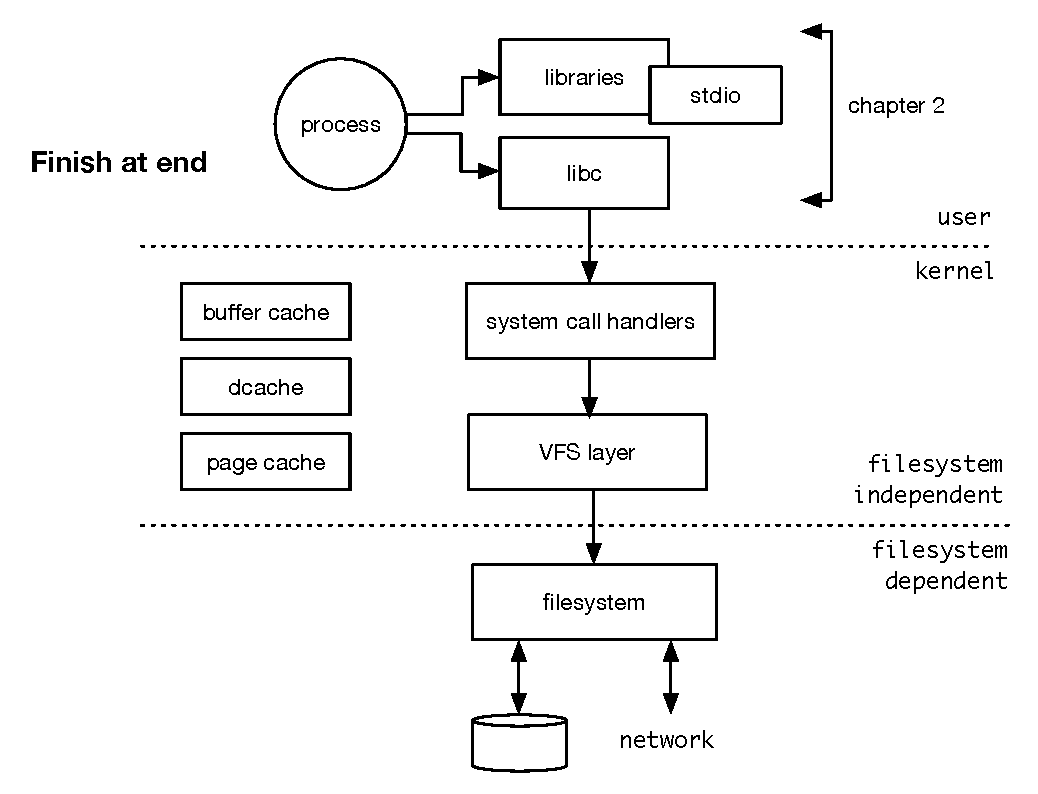
\includegraphics[scale=0.6]{figures/intro-figure.pdf}
	\centering
	\caption{Various subsystems in Linux and their location in the book}
	\label{fig:intro-figure}
\end{figure}

The book concludes with chapters on debugging techniques, file system performance and filesystem security. Figure \ref{fig:intro-figure} highlights the parts of a Linux operating system and where each is covered in the book. In more detail, here is the breakdown of each chapter:

\begin{itemize}
	\item{\textbf{Chapter 1 -- Introduction}} -- This chapter.
	\item{\textbf{Chapter 2 -- File and Filesystem Programming}} -- before understanding how the Linux kernel provides support
		for filesystems and file access, it's necessary to explore the different commands, system calls and 
		library functions that applications use to access files and filesystems. This chapter provides information
		on the Linux standards followed, manual pages (manpages), file types, programming interfaces, 
		sparse files and various types of I/O including direct I/O and asynchronous I/O. The standard I/O
		library is discussed in detail with information about how to browse the standard library source code.
		There is a section on reading directory entries with a simple implementation of the \cf{ls(1)} command.
	\item{\textbf{Chapter 3 -- Filesystems}} -- this chapter covers everything from the different file systems that 
		Linux provides to the operations that can be applied to them such as mounting, unmounting and reporting 
		disk usage. Physical and pseudo filesystems will be described together with highlights of network 
		and FUSE-based file systems including a demonstration of SSHFS which allows you to view remote 
		files as if they were mounted locally. We will also cover backup and restore, quotas, swap space and 
		how the boot process works in terms of filesystem access.
	\item{\textbf{Chapter 4 -- A First Look at the Linux Source Code}} -- with 25 million lines of source code, the 
		Linux kernel is one very large piece of code and can be daunting, especially if you've never spent much 
		or any time looking at it! The chapter describes the layout of the source code and focuses on where the
		main file and filesystem structures and routines can be found. It describes various tools that can
		be used to navigate around the source code from the simple such as \cf{vim} and tag stack to 
		the more complete solutions such as \cf{cscope(1)} and Elixir. The chapter then describes the
		main structures that related to filesystems and show how the structures are linked together. The
		main routines will be highlighted together with a few simple examples and browsing through
		kernel structures using \cf{gdb}.
	\item \textbf{Chapter 5 -- Common Linux Types} -- \textbf{TBD}
	\item \textbf{Chapter 6 -- The VFS Layer} -- Following on from the previous chapter which covered the main 
		structures related to filesystems, this chapter goes much deeper in explaining the code paths through the
		kernel functions to respond to the various filesystem related system calls.
	\item \textbf{Chapter 7 -- Filesystem Case Studies} -- \textbf{TBD}
	\item{\textbf{Chapter 8 -- Building a Kernel-based Filesystem}} -- this is a fun chapter! It presents a fully 
		functional, disk-based file system that contains less than 1500 lines of source code. The foul system was 
		developed on Ubuntu Linux but should be able to run on any version of Linux. It comes with tools 
		for making a file system and a file system debugger. Volatile system is very simple in nature it 
		does support the majority of foul system operations. For fun it also includes an undelete command.
	\item{\textbf{Chapter 9 -- The FUSE Filesystem Framework}} -- the FUSE implementation in the Linux kernel 
		allows developers to implement file systems in user a space. This chapter provides two examples for 
		FUSE, one which provides a pass-through set of operations reflecting what is under the file system on 
		which it is mounted. The second example builds on the first by providing encryption of files and file names 
		using very simple key management. The implementation of the FUSE architecture will be presented 
		together with information about performance gains that have been achieved over the years including 
		some new performance enhancements using eBPF.
	\item{\textbf{Chapter 10 -- Filesystem Debugging}} -- debugging kernel code is certainly a challenge. 
		Application developers have an array of filesystem debug us to choose from including \cf{gdb}. In my 
		career I've spent many a year debugging file system code at assembler level which can be fun but not for 
		the faint hearted. This chapter covers debugging the kernel at source level using GDP but also explores a 
		number of other different debugging techniques including the more recent and very powerful eBPF tools.
	\item{\textbf{Chapter 11 -- Filesystem Performance}} -- they have been many books written about UNIX and 
		Linux performance over the years. Although this book won't go into the detail that other books and 
		articles online have covered but this chapter will explore the main performance related aspects of 
		file access and in particular some of the new eBPF performance tools.
	\item{\textbf{Chapter 12 -- Filesystem Security}} -- security is a very large topic and there are many tools, 
		standards and practices for securing file system data. This chapter highlights the bank security concerns 
		with foul and foul system access and describes everything from standard UNIX file permissions to 
		encryption key management. Security based sub systems like SELinux and AppArmor are 
		also explored.
\end{itemize}

%%%%%%%%%%%%%%%%%%%%%%%%%%%%%%%%%%%%%%%%%%%%%%%%%%%%%%%%%%%%%%%%%

\section{Why is Source Code Missing?}

There are many examples throughout the book where I only display part of a kernel structure, part of a function or even strip down some functions to remove error checking and other parts of the function. The goal behind this is to show the most relevant structures and fields and the most prominent paths through functions. I think this is preferable to putting in large amounts of source code and making it harder to see the big picture. Just bear this in mind when browsing the kernel source.

%%%%%%%%%%%%%%%%%%%%%%%%%%%%%%%%%%%%%%%%%%%%%%%%%%%%%%%%%%%%%%%%%

\section{KGDB Demonstrations}

In various sections throughout the book you will see headings such as:

\begin{quote}
\textbf{4.2.1 KGDB --- Analyzing Per-file Kernel Structures}
\end{quote}

\noindent
In these sections, I use \cf{gdb} and the kernel source-level debugger stub \cf{kgdb} to demonstrate the subject matter being displayed. There are also online videos on my YouTube channel showing more detailed versions that I recommend you watch. All  demonstrations will help reinforce the material presented.

Generally speaking, when I demonstrate an area of the kernel using \cf{gdb} there will be an accompanying YouTube video

\begin{table}[h]
\begin{tabular}{ll}
\parbox[l]{0.6in}{
\includegraphics[scale=0.3]{figures/video-camera.pdf}} & \parbox[l]{4in}{\small{\textbf{VIDEO 2} -- Analyzing VFS structures for open files}}
\end{tabular}
\end{table}

\noindent
If you look at the list of video references on my website, it will be easy to see the number and be able to click on the link. I thought this would be easier than putting URLs in here.

Before looking through the kgdb examples, I'd recommend that you read the section \ref{kgdb} first. Even if you skip all the steps to set up kgdb, look at the command and examples to understand the process that's being followed. 

In all examples, I'm going to make use of what \cf{gdb} calls \textit{convenience variables} that reference the structures that are being analyzed. No one can remember long memory addresses and I think this is the easiest way to help with understanding the flow. It's not the quickest method and there will be scripts to help with that. \textbf{XXXX-maybe / maybe not}

%%%%%%%%%%%%%%%%%%%%%%%%%%%%%%%%%%%%%%%%%%%%%%%%%%%%%%%%%%%%%%%%%

\section{Source Code Figures}[h]

There are several different ways that source is described throughout the book. Often the code is just printed as is. Sometimes, only relevant parts of a function are described and there many times during which \cf{gdb} is used to display stack backtraces which help to understand how certain functions are reached.

I find it helpful to use a drawing package to add code fragments and arrows showing how they're all connected. I use OmniGraffle, a drawing package that I've used for many years. Figure \ref{fig:code-walkthrough} gives an example of such a figure.

\begin{figure}[h]
	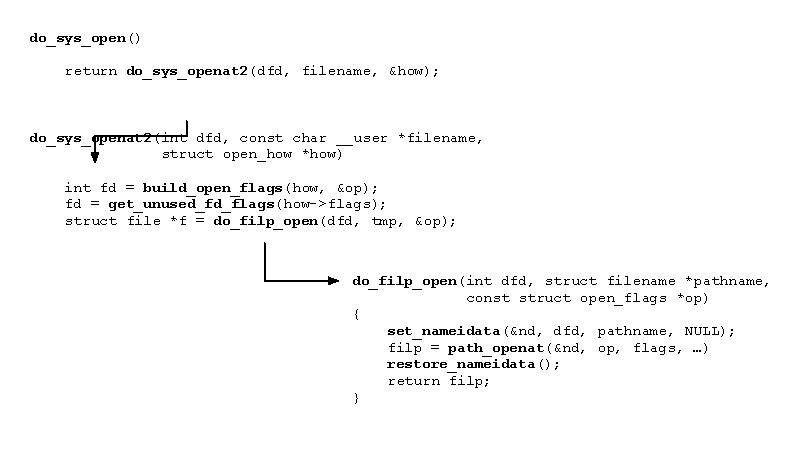
\includegraphics[scale=0.64]{figures/code-walkthrough.pdf}
	\centering
	\caption{Example Figure Showing Code Paths through the Linux Kernel}
	\label{fig:code-walkthrough}
\end{figure}

A few of these figures are shown throughout the book but rarely with this much detail. To help your understanding of how the Linux kernel works, I've collected several of these figures together. You can download them from my website -- \textbf{details TBD}

%%%%%%%%%%%%%%%%%%%%%%%%%%%%%%%%%%%%%%%%%%%%%%%%%%%%%%%%%%%%%%%%%

\section{Acknowledgements}

First and foremost, a big thank you to Eleanor who encouraged me to work on book writing full-time, which is quite a commitment. It's now almost 30 years since the publication of my first book. I've really enjoyed the process in the past but to be able to do it full time rather than cram it into evenings and weekends has made the process much more enjoyable.

Thanks to \textbf{xxx and yyy} for reviewing the material. 

Thanks to Lukas Brand who sent me an article about filesystem security. While planning the book, I forgot that I'd been in the security industry working on filesystem and device encryption for the last 15 years!

\textbf{TBD --- do this last}




\chapter{File and Filesystem Programming}

% https://tldp.org/LDP/intro-linux/html/sect_03_04.html - chmod / file masks etc this stuff should go in the programming chapter or somewhere else

Before diving into the Linux kernel to understand how files and filesystems are accessed and how filesystems operate internally, it's best to look at what's happening in user space by understanding how applications access files. Much of what the kernel does is to satisfy a set of system calls (functions in the kernel that programs access). A process, which is the running instantiation of an executable program, either access this set of system calls directly or uses a set of library functions which in turn use the system call interface.

This chapter explores all the different ways that applications can access files from basic \cf{read(2)} and \cf{write(2)} system calls to the standard I/O library to asynchronous I/O and less-used features such as extended attributes. 

\section{Programming Standards and Portability}

Around the time of my last book, we were still living in a world of multiple different UNIX and UNIX-variants of which Linux was one key player. Over the years, there have been several standards bodies created to develop a common set of programming interfaces that each of the operating system vendors diligently worked to adopt to make the life of application developers much easier. I remember working with several dedicated people attending standards meetings of one form or another, implementing these changes and ensuring that the interfaces adhered to the standard by using a common set of test suites.

With Linux and Windows now dominating approximately 90\% of the server operating system market, there are only really two platforms now to consider and a relatively small number of Linux distributions covering all Linux installed systems. Of course if we consider smart phones and tablets, that means Android (also Linux based) and iOS. Although these applications are very different from those in the server world, application portability is still important. Wherever possible, you should use standard interfaces. Having a high-level of portability across not just Windows and Linux but Apple OS/X and the various BSD operating systems is still a smart choice.

It's beyond the scope of this book to discuss all the issues around source code portability but I wanted to at least highlight the different standards that are our there to make you aware before you delve into writing a complex application. Think about where that application may end up in future even if operating system portability isn't a goal initially. You will want to think carefully about the toolchain that you'll use as part of the development process. 

The Linux manual pages indicate which standard the functions they describe adhere to. Let's take three examples. Starting with the \cf{write(2)} system call:

\begin{lstlisting}
CONFORMING TO
	   SVr4, 4.3BSD, POSIX.1-2001.
\end{lstlisting}

\noindent 
For the \cf{printf(3)} library function:

\begin{lstlisting}
CONFORMING TO
	fprintf(), printf(), sprintf(), vprintf(), vfprintf(),
	vsprintf(): POSIX.1-2001, POSIX.1-2008, C89, C99.

	snprintf(), vsnprintf(): POSIX.1-2001 & 2008, C99.

	dprintf() and vdprintf() functions were originally GNU
	extensions and were later standardized in POSIX.1-2008.
\end{lstlisting}

\noindent
The \cf{getenv(3)} manual page is a little different. It also describes \cf{secure\_getenv()} which it states "\textit{is a GNU extension}":

\begin{lstlisting}
CONFORMING TO
	getenv(): POSIX.1-2001, POSIX.1-2008, C89, C99, 
	          SVr4, 4.3BSD.

	secure_getenv() is a GNU extension.
\end{lstlisting}

\noindent 
This could mean that it's not portable across different operating systems so be careful of such extensions.

\subsection{What are all These Standards?}

There have been many attempts at standardization over the last few decades. Here are the prominent staandards and how they relate to Linux:

\begin{itemize}
	\item POSIX --- The Portable Operating System Interface (POSIX and pronounced \textit{pahz-icks}) 
		is a family of standards specified by IEEE. It defines both system- and user-level "\textit{Application 
		Programming Interfaces}" (APIs), along with command line shells and utility interfaces, for software 
		compatibility (portability) with variants of UNIX and other operating systems. 
	\item Single UNIX Specification (SUS) --- a standard that specifies programming interfaces for the C language, 
		a command-line shell, and user commands. Conformance with SUS allowed operating systems vendors
		to use the name 'UNIX" as part of their brand offering. What started out as \textit{Spec 1170}, a
		set of 1,170 commands/interfaces, the collection of all such interfaces would eventually become the Single Unix Specification.
		Very few Linux and BSD vendors/distributions have gone through certification and with the number of UNIX versions declining, 
		we are unlikely to see any more.
	\item C89 - C2x --- ANSI C - standards for the C programming language. As you can see from the manual pages
		of three functions above, many Linux functions state compliance. 
	\item Linux Standard Base (LSB) --- formed by the Linux Foundation, LSB was a joint project 
		comprising multiple Linux distributions with the goal to standardize Linux software system structure, 
		including the \textit{Filesystem Hierarchy Standard} used in the Linux kernel. LSB was based 
		on the POSIX specification, the Single UNIX Specification (SUS), and several other open standards, 
		but it also extended them in some areas.
\end{itemize}

\noindent
The first version of POSIX.1 was published in 1988 and the most recent in 2017. Prior to 1997, POSIX was split into several different sub-standards which I'm listing in full below to show how extensive the standard actually was. I recall working on an implementation of threads on an SVR4 UNIX subsystem on the Chorus microkernel while the standard was still being developed back in the early 1990s.

\begin{itemize}
	\item POSIX.1: Core Services (incorporates Standard ANSI C) 
		\begin{itemize}
			\item Process Creation and Control
			\item Signals
			\item Floating Point Exceptions
			\item Segmentation / Memory Violations
			\item Illegal Instructions
			\item Bus Errors
			\item Timers
			\item File and Directory Operations
			\item Pipes
			\item C Library (Standard C)
			\item I/O Port Interface and Control
			\item Process Triggers
		\end{itemize}
	\item POSIX.1b: Real-time extensions
		\begin{itemize}
			\item Priority Scheduling
			\item Real-Time Signals
			\item Clocks and Timers
			\item Semaphores
			\item Message Passing
			\item Shared Memory
			\item Asynchronous and Synchronous I/O
			\item Memory Locking Interface
		\end{itemize}
	\item POSIX.1c: Threads extensions
		\begin{itemize}
			\item Thread Creation, Control, and Cleanup
			\item Thread Scheduling
			\item Thread Synchronization
			\item Signal Handling	
		\end{itemize}
	\item POSIX.2: Shell and Utilities
		\begin{itemize}
			\item Command Interpreter
			\item Utility Programs
		\end{itemize}
\end{itemize}

\noindent
After the first version of POSIX in 1988, there have been several other enhanced versions namely, POSIX.1-2001, POSIX.1-2008 and the final version, POSIX.1-2017. There is a nice FAQ on POSIX by the OpenGroup here if you wish to read further:

\begin{table}[h]
\begin{tabular}{lcl}
\parbox[r]{0.5in}{ 
\includegraphics[scale=0.15]{figures/url.png}} & \parbox[l]{0.1in}{\arabic{urls}} & \parbox[l]{3in}{\cf{https://tinyurl.com/5bnxjrae}}
\end{tabular}
\end{table}
\stepcounter{urls}
% https://www.opengroup.org/austin/papers/posix_faq.html

\subsection{LSB --- Linux Standard Base}

The Linux Standard Base covered everything from standard libraries, commands and utilities that extended the POSIX standard, file system hierarchy layout, run levels, X Window System extensions, System V UNIX-style initialization scripts and others. Version 1.0 of LSB was released in 2001 and the last version (5.0) in 2015. There were 21 release versions of Linux certified for LSB 4.0 but considerably fewer for 4.1.

LSB has certainly had its critics over the years. Apparently LSB 3.0 was released with a big yawn and also had critics from the glibc team for which it created a lot of additional work. One of the original goals of LSB was for application compatibility allowing 3rd party developers to write-once, run-anywhere including binary and package levels. The goals were sound with Linux leaders not wanting Linux distributions to diverge as the various UNIX vendors had in the past. 

Nowadays, relatively few Linux distributions dominate the landscape which reduces the demands for something like LSB and proprietary vendors tend to target specific distributions based on demands from their customer base. But LSB was largely successful in that it brought Linux vendors together at a time that divergence was a real possibility.

At the time of writing, the \cf{lsb\_release(1)} command, which did display LSB version details, now just displays information specific to the Linux release. As an example, for Ubuntu:

\begin{lstlisting}
$ [*\bfseries lsb\_release -a*]
No LSB modules are available.
Distributor ID:	Ubuntu
Description:	Ubuntu 22.10
Release:	22.10
Codename:	kinetic
\end{lstlisting}

\section{Manual Pages}

All functions that can be used by an application that are provided by the operating system have a corresponding manual page which is more commonly referred to as a "\textit{manpage}". For programming interfaces, the manpage documents expected parameters, return values and header files that need to be included. There are also manpages for all of the Linux commands, file formats and so on. You can do a keyword search to find manpages that are relevant to the keyword that you supply. For example, let's search for write-related man pages.

Below is a subset of what is shown when searching for write-related functions and commands. There is a command called \cf{write} as indicated by \cf{(1)} and the \cf{write} system call as indicated by \cf{(2)}.

\begin{lstlisting}
$ [*\bfseries man -k write*]
aio_write (3)        - asynchronous write
fwrite (3)           - binary stream input/output
pwritev (2)          - read or write data into multiple buffers
write (1)            - send a message to another user
write (2)            - write to a file descriptor
...
\end{lstlisting}

\noindent
What do the numbers in parenthesis mean? The UNIX (and now Linux) manual pages are divided into different sections. The section for each manpage is shown above in parenthesis. To see the list of available sections, you can run "\cf{man man}". Here are the nine sections for Linux:

\begin{lstlisting}
1   Executable programs or shell commands
2   System calls (functions provided by the kernel)
3   Library calls (functions within program libraries)
4   Special files (usually found in /dev)
5   File formats and conventions, e.g. /etc/passwd
6   Games
7   Miscellaneous (including macro packages and conventions),
	e.g. man(7), groff(7), man-pages(7)
8   System administration commands (usually only for root)
9   Kernel routines [Non standard]
\end{lstlisting}

\noindent
If you want to display the man page for the \cf{write()} system call, run "\cf{man 2 write}". If you want to see the "\cf{printf()}" manpage run "\cf{man printf(3c)}". And if you're unsure which section you need, use the "\cf{-k}" option. 

I have on occasion run into issues when trying to view manpages, specifically those related to programming. For example, if you see an error when running "\cf{man 2 open}" you need to install the development manpages as follows:

\begin{lstlisting}
$ [*\bfseries {sudo apt install manpages-dev*]
\end{lstlisting}

\noindent
There is a wealth of information in the Linux manpages. If you don't have a running system at hand, just enter "\cf{write(2)}" in your favorite search engine and you'll be able to view it online.

\section{System Calls vs Library Functions -- an Overview}

A software library is just a collection of source code functions and variables that are combined together into a single \textit{library file}. The library can't run by itself. When user programs are built, the source code is first compiled then it is \textit{linked} with one or more libraries to make an executable or binary.

When writing applications you will likely use a number of different library functions. Just take the first program that people usually write in C (or most other languages):

\begin{lstlisting}
#include <stdio.h>

int 
main()
{
	printf("Hello world!\n");
}
\end{lstlisting}

\noindent
The program can be compiled as follows to get an executable:

\begin{lstlisting}
$ [*\bfseries cc hello\_world.c -o hello\_world*]
\end{lstlisting}

\noindent
or "\cf{make hello\_world}" will achieve the same result. In this program we use a single library function called \cf{printf(3)} that is contained in what is known as the \textit{standard C library} (see \cf{libc7} for more information). To see what libraries our executable program is linked with, we can use the \cf{ldd(1)} command as follows:

\begin{lstlisting}
$ [*\bfseries ldd hello\_world*]
linux-vdso.so.1 (0x0000ffffb4e83000)
libc.so.6 => 
/lib/aarch64-linux-gnu/libc.so.6 (0x0000ffffb4c70000)
/lib/ld-linux-aarch64.so.1 (0x0000ffffb4e46000)
\end{lstlisting}

If library functions are just functions packaged together, what is the difference between a library function and a system call? When writing applications you use library functions which may perform the required function by themselves or they may call into the Linux kernel for services. For a simple program such as the one below, you may unaware of difference between one function type and another (error checking excluded for simplicity):

\begin{lstlisting}
#include <fcntl.h>
#include <stdio.h>
#include <unistd.h>
#include <string.h>

int
main()
{
    char buf[64];
    int  fd;

    fd = [*\bfseries open*]("msg", O_CREAT | O_WRONLY);
    [*\bfseries sprintf*](buf, "hello world -> fd = %d\n", fd);
    [*\bfseries write*](fd, buf, [*\bfseries strlen(buf)*]);
}

\end{lstlisting}

\noindent
There are four different functions called two of which are system calls (\cf{open} and \cf{write}) and two which are not. As programmers gain experience they will generally know which functions are system calls and which are not without having to check the manpages. Later sections in the book will describe system call handling for file and filesystem-related functions in detail.

\section{Error Handling with \cf{errno}}

As the \cf{errno(3)} manpage says:

\begin{quote}
\textit{The  <errno.h> header file defines the integer variable errno, which is set by system calls and some library functions in the event of an error to indicate what went wrong.}
\end{quote}

\noindent       
If you're like me, trying to remember error codes and which \cf{errno} value they correspond to, good luck! However, if you install the \cf{moreutils} package, you have a handy utility at your disposal:

\begin{lstlisting}
$ [*\bfseries sudo apt install moreutils*]
$ [*\bfseries errno 9*]
EBADF 9 Bad file descriptor
$ [*\bfseries errno EBADF*]
EBADF 9 Bad file descriptor
\end{lstlisting}

\noindent
I also have a simple script that dumps all of them out:

\begin{lstlisting}
echo "number    hex symbol  description
1   0x01    EPERM   Operation not permitted
2   0x02    ENOENT  No such file or directory
...
132 0x84    ERFKILL Operation not possible due to RF-kill
133 0x85    EHWPOISON   Memory page has hardware error "
\end{lstlisting}

\noindent
Note that the actual error values are not stored in \cf{/usr/include/errno.h} but can be found in \cf{/usr/include/asm-generic/errno-base.h}.

\section{File Types and Mode}

Everything stored in a Linux filesystem is a file regardless of the file type. Here are the different types of files that can be supported by Linux although note that not all filesystems support all file types. For example, the BFS filesystem is a specialized SVR4 UNIX filesystem for supporting boot-related files including the kernel. It is a flat filesystem so it doesn't support creation of directories (although it does have a root directory):

\begin{enumerate}
	\item \textbf{Regular files} --- a file that contains data that applications create and interpret. The filesystem 
		or the kernel has no knowledge about the content of regular files. 
	\item \textbf{Directory files} --- also called \textit{folders} (although primarily in desktop operating systems such
		as Windows and OS/X), a directory can contain files and other directories.
	\item \textbf{Symbolic links} --- a file that contains a pathname that references another file. It could be a 
		single name or multiple names separated by "/". A symbolic link can point anywhere in the Linux 
		filesystem namespace. It does not have to point to a file within the same filesystem.
	\item \textbf{Hard links} --- a name within a directory that references another file's contents and meta-data 
		directly. If file '\cf{a}' is a hard link to file '\cf{b}' and if you delete file '\cf{b}', you can still access the file through '\cf{a}'. For
		a symbolic link, If file '\cf{a}' is a symbolic link to file '\cf{b}' and if you delete file '\cf{b}', you cannot still access the 
		file through '\cf{a}'.
	\item \textbf{Device nodes} --- a special file that contains both a \textit{major} number which is used to
		reference a specific device driver and a \textit{minor} number that it interpreted by the device driver.
		For example, on my Ubuntu VM there are two device nodes for a specific SCSI disk:
		\begin{lstlisting}
brw-rw---- 1 root disk 8, 1 Dec 15 16:41 /dev/sda1
brw-rw---- 1 root disk 8, 2 Dec 15 16:41 /dev/sda2
\end{lstlisting}
		The major number is \cf{8} which references the SCSI device driver and the minor numbers \cf{1} 
		and \cf{2} are used by the device driver to refer to specific partitions. Note that we can have block 
		and character special files. A Character Device is a device for which the device driver reads and 
		writes single characters. Examples include keyboards, serial and parallel ports. A Block Device 
		is a device for which the device driver reads/writes blocks of data. An example would be hard 
		disks. Note that filesystems can only reside on block devices.
	\item \textbf{Sockets} --- a special file used for inter-process communication between two processes. 
		In addition to sending data, processes can send file descriptors across a UNIX domain socket 
		using the \cf{sendmsg(2)} and \cf{recvmsg(2)} system calls.
	\item \textbf{FIFOs}  --- also called a \textit{named pipe}, a FIFO is a uni-directional channel through
		which one process can send data and another process can receive it. Pipes/FIFOs are created
		by the \cf{mkfifo(1)} command.
\end{enumerate}

\noindent
You can find out the type of a file by using the \cf{stat(1)} command or one of 4 different system calls namely \cf{stat}, \cf{lstat}, \cf{fstat} and \cf{fstatat} all which are described in the \cf{stat(2)} manpage. The \cf{st\_mode} field returned by these functions contains both the file type and the file mode. To understand more about the mode, the \cf{inode(7)} manpage explains how each file can be identified. We'll also cover system calls in more detail soon.

\begin{lstlisting}
S_IFMT     0170000   bit mask for the file type bit field

S_IFSOCK   0140000   socket
S_IFLNK    0120000   symbolic link
S_IFREG    0100000   regular file
S_IFBLK    0060000   block device
S_IFDIR    0040000   directory
S_IFCHR    0020000   character device
S_IFIFO    0010000   FIFO
\end{lstlisting}

\noindent
Below is a short program that calls \cf{stat(2)} on a regular file. We print out the \cf{st\_mode} field and with the mask so we can just determine the file type.

\begin{lstlisting}
struct stat buf;
int error = stat("lorem-ipsum", &buf);

printf("mode = %o (%o)\n", buf.st_mode, buf.st_mode & S_IFMT);
if (S_ISREG(buf.st_mode)) {
	printf("The file is a regular file\n");
}
if ((buf.st_mode & S_IFMT) == S_IFREG) {
	printf("... and again!\n");
}
\end{lstlisting}

\noindent
The program then use two different methods to check to see if this is a regular file.

\begin{lstlisting}
$ [*\bfseries ./st*]
mode = 100644 (100000)
The file is a regular file
... and again!
\end{lstlisting}

\noindent
The remainder of the \cf{st\_mode} field is for storing the file's permissions. In this case we have \cf{644} which we can see when running \cf{ls(1)}. Figure \ref{fig:ls-l} also shows several components of a file displayed by running "\cf{ls -l}". Permissions show access rights by user, group and others.

\begin{figure}[h]
	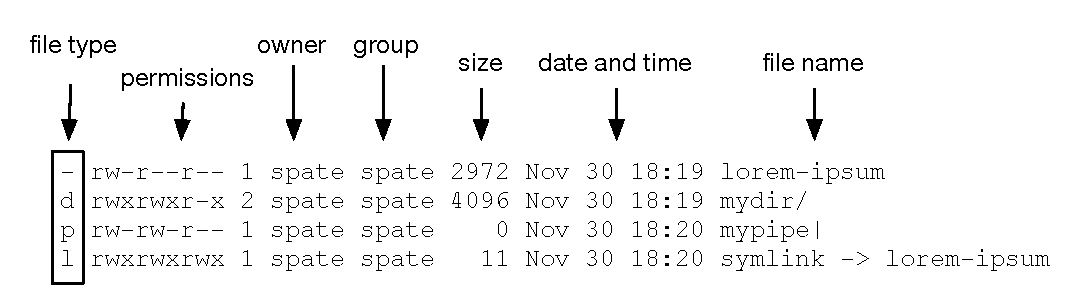
\includegraphics[scale=0.6]{figures/ls-l.pdf}
	\centering
	\caption{The Components of a File as Shown by Running \cf{ls -l}}
	\label{fig:ls-l}
\end{figure}

\section{File Descriptors}

Every time a file is opened or a file is created, a file descriptor is returned that can be used to reference the open file through uses of one of several different operations such as \cf{read(2)}, \cf{write(2)} and \cf{lseek(2)}. File descriptors are allocated on a per-process basis and are always non-negative. The first 3 file descriptors are reserved as shown in table \ref{table:fds}.

\begin{table}[h]
\begin{center}
\begin{tabular}{|p{0.1\textwidth}|m{0.1\textwidth}|m{0.3\textwidth}|m{0.3\textwidth}|}
\hline
\rowcolor[gray]{.93}\bf{Name}&\bf{Value}&\bf{<stdio.h> file stream}&\bf{\cf{<unistd.h>} constant}\\
\hline
\cf{stdin}&0&standard input&\cf{STDIN\_FILENO}\\
\hline
\cf{stdout}&1&standard output&\cf{STDOUT\_FILENO}\\
\hline
\cf{stderr}&2&standard error&\cf{STDERR\_FILENO}\\
\hline
\end{tabular}
\caption{\small Standard File Descriptors}
\label{table:fds}
\end{center}
\end{table}

\noindent
In the example below, you can see that the following program will receive the next available file descriptor which is 3.

\begin{lstlisting}
$ [*\bfseries cat fd.c*]
#include <stdio.h>
#include <fcntl.h>

int
main()
{
	int fd = open("lorem-ipsum", O_RDONLY);
	printf("fd = %d\n", fd);
}
$ [*\bfseries make fd*]
$ [*\bfseries ./fd*]
fd = 3
\end{lstlisting}

\noindent
Jumping ahead a little to demonstrate how file descriptors are used in the kernel, the \cf{read(2)} system call us handled by the kernel function \cf{ksys\_read()} of which I've included a fragment of the source code here:

\begin{lstlisting}
ssize_t [*\bfseries ksys\_read*](unsigned int fd, char __user *buf, 
                  size_t count)
{   
	struct fd f = [*\bfseries fdget\_pos*](fd);
	loff_t pos, *ppos = [*\bfseries file\_ppos*](f.file);
	ret = [*\bfseries vfs\_read*](f.file, buf, count, ppos);
\end{lstlisting}

\noindent
As you can see, the arguments are very similar to the \cf{read(2)} system call. Inside this function the kernel uses the file descriptor to get an \cf{fd} struct. From there, it gets the position from the last read (or seek) and calls \cf{vfs\_read()} to continue read processing. We'll explore the kernel side of reading later in section \cf{XXX}.

%------------------------------------------------------------------------------------------------------------------------------------------------------------

\subsection{How Many Open Files?}

Most applications only open a small number of files and the Linux kernel is set up to support this by default for each process. The \cf{getdtablesize(2)} manpage has conflicting information. It states that it returns the maximum number of files a process can have open. But then it lists the return value as the \textit{current limit}. The following program retrieves this value and also checks to see what is returned from calling \cf{getrlimit()} which returns both the current limit (also called the \textit{soft limit}) and the \textit{hard limit} as returned by calling \cf{getrlimit(2)}:

\begin{lstlisting}
#include <unistd.h>
#include <stdio.h>
#include <sys/resource.h>

int
main()
{
    struct rlimit  rlim;
    int            nentries;

    nentries = getdtablesize();
    getrlimit(RLIMIT_NOFILE, &rlim);
    printf("Current file table entries = %d\n", nentries);
    printf("rlimit current / maximum = %d / %d\n",
           (int)rlim.rlim_cur, (int)rlim.rlim_max);
}
\end{lstlisting}

\noindent
Here is what we get when running the program. 1,048,576 is certainly larger than most applications will need.

\begin{lstlisting}
Current file table entries = 1024
rlimit current / maximum = 1024 / 1048576
\end{lstlisting}

\noindent
You can also get the current limit by calling the shell built-in command "\cf{ulimit -Sn}" and calling "\cf{ulimit -Hn}" to get the hard limit.

%------------------------------------------------------------------------------------------------------------------------------------------------------------

\subsection{Closing Files}

There isn't a great deal to say about closing files. The system call, as described in \cf{close(2)} is as follows:

\begin{lstlisting}
#include <unistd.h>

int close(int fd);
\end{lstlisting}

\noindent
If there are any record locks held on the file that \cf{fd} refers to and are owned by the calling process, they are removed.

If \cf{fd} is the last file descriptor referring to the underlying open file any resources that associated with the open file are freed. If the file descriptor is the last reference to a file which has been removed by a prior call to \cf{unlink(2)}, the file will then be deleted. The latter point is an interesting one for filesystem developers as the file could remain in this state for an extended period of time and there are certainly implications if the system is restarted in between these two operations.

%------------------------------------------------------------------------------------------------------------------------------------------------------------

\subsection{Duplicating File Descriptors}

The \cf{dup(2)} system call can be called to allocate a new file descriptor which will reference the same open file as the descriptor \cf{oldfd}. The returned value is guaranteed to be the lowest-numbered file descriptor that is unused in the calling process.

\begin{lstlisting}
#include <unistd.h>

int dup(int oldfd);
int dup2(int oldfd, int newfd);
\end{lstlisting}

\noindent
Since both old and new file descriptors reference the same file, they can then be used interchangeably.  They also share file offset and file status flags. If the file offset is changed by using the \cf{lseek(2)} system call on one of the file descriptors, the offset will also changed for the other file descriptor.

The \cf{dup2(2)} system call is similar but instead of getting the lowest available file descriptor, the file descriptor specified by \cf{newfd} is used. If \cf{newfd} is currently in use, it is closed first. This function is the equivalent of calling \cf{fcntl(2)} and passing the \cf{F\_DUPFD} command.

The \cf{dup3(2)} system call was added to Linux version 2.6.27. It performs the same function as \cf{dup2(2)} with one exception. The caller can force the close-on-exec flag to be set  for  the  new file  descriptor by setting \cf{flags} to \cf{O\_CLOEXEC}.  In this case the file descriptor will be closed following a call to \cf{execve(2)}. The \cf{open(2)} manpage describes how this flag is useful in multithreaded applications.

\begin{lstlisting}
#include <fcntl.h> 
#include <unistd.h>

int dup3(int oldfd, int newfd, int flags);
\end{lstlisting}

\noindent
The most common use case for duplicating file descriptors is to connect processes via a pipe which is a common operation we all use when running one command in the shell and connecting the output to the input of the next command. In the following example:

\begin{lstlisting}
$ [*\bfseries find . -name *.c | xargs grep myfunc*]
\end{lstlisting}

\noindent
the output of the \cf{find} command is connected to the input of the \cf{xargs} command.

\subsubsection{An Example of Redirection}

This section is really going beyond the scope of this book but redirection is such a fundamental part of the UNIX/Linux shell, that I thought it was worth taking a slight diversion for readers who may not be familiar with how pipes are used to achieve one of UNIX's most fundamental and wonderful capabilities. 

Take a look at the following commands connected together where the standard output of \cf{echo} is connected to the standard input of \cf{cat}:

\begin{lstlisting}
$ [*\bfseries echo "Hello world" | cat*]
Hello world
\end{lstlisting}

\noindent
Below is a program that forks/execs two other programs (\cf{myecho} and \cf{mycat}) and uses a combination of \cf{dup(2)} and \cf{pipe(2)} to connect the two processes together through \cf{stdin} and \cf{stdout} in a simple but similar way to how the shell operates. When the \cf{shell} program is run we'll see our message displayed:

\begin{lstlisting}
$ [*\bfseries ./shell*]
Hello world!
\end{lstlisting}

\noindent
To see this visually, refer to figure \ref{fig:pipe}.

\begin{figure}
	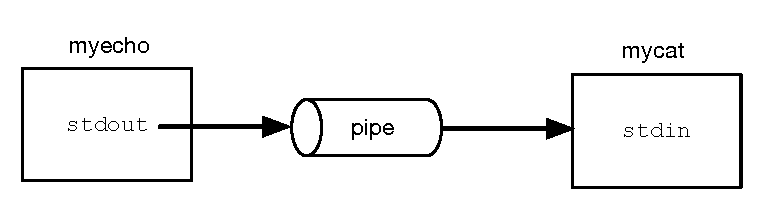
\includegraphics[scale=0.6]{figures/pipe.pdf}
	\centering
	\caption{Tow processes connected via a pipe}
	\label{fig:pipe}
\end{figure}

Below is the \cf{shell} program. As per usual, we've left out error checking for the purpose of keeping the number of lines as small as possible.

\begin{lstlisting}
 1 #include <unistd.h>
 2 #include <stdlib.h>
 3 #include <stdio.h>
 4 
 5 int main(int argc, char **argv) {
 6     int   pipefd[2];
 7     pid_t child;
 8 
 9     pipe(pipefd);
10     child = fork();
11  
12     if (child == 0) {
13         /* child process */
14         close(STDOUT_FILENO);
15         dup(pipefd[1]);
16         execlp("myecho", "myecho", "Hello world!\n",
17                (char *)NULL);
18     } else {
19         /* parent process */
20         close(STDIN_FILENO);
21         dup(pipefd[0]);
22         execlp("mycat", "mycat", (char *)NULL);
23     }
24 }
\end{lstlisting}

\noindent
The following bullet points describe what the various parts of the program are doing (line numbers are on the left):

\begin{itemize}
	\item line 9 -- A pipe is created where  \cf{pipe[0]} is the file descriptor through which we can read data
		and \cf{pipe[1]} is the file descriptor through which we can write data.
	\item line 10 -- The program is forked.
	\item line 14 -- \cf{stdout} is closed for the \cf{myecho} process.
	\item line 15 -- \cf{dup(2)} is called to duplicate the file descriptor in \cf{pipefd[1]} which is the \textit{write side}
		of the pipe. Recall that \cf{dup(2)} is guaranteed to return the lowest-numbered file descriptor that
		unused in the calling process. Since we have just closed \cf{stdout} which has a file descriptor of \cf{1},
		\cf{dup(2)} file descriptor 1 will be used which is \cf{stdout}.
	\item line 16 -- At this point we exec the \cf{myecho} program and pass \cf{"Hello world!"} as an argument.
	\item line 20 -- \cf{stdin} for the \cf{mycat} process is closed.
	\item line 21 -- Similar to line 15, we replace \cf{stdin} for \cf{mycat} with the \textit{read side} of the pipe.
	\item line 22 -- Finish with a call to exec the \cf{mycat} program.
\end{itemize}

\noindent
The actual shell is of course considerably more complicated than this program but in essence, this is what it is doing. 

Here is the \cf{myecho} program. It's very simple and just writes the argument passed to \cf{stdout}.

\begin{lstlisting}
#include <stdio.h>

int
main(int argc, char *argv[])
{
    fprintf(stdout, "%s", argv[1]);
}
\end{lstlisting}

\noindent
Here is the \cf{mycat} program. It reads from \cf{stdin} and writes the output (to \cf{stdout}.

\begin{lstlisting}
#include <stdio.h>
#include <string.h>

#define BUFSZ 64

int
main()
{
    char buf[BUFSZ];

    fgets(buf, BUFSZ, stdin);
    printf("%s", buf);
}
\end{lstlisting}

\noindent
Note that if you run these programs, make sure that \cf{PATH} is set to include the current directory so that the \cf{myecho} and \cf{mycat} programs can be found.

If you remove the comments around \cf{fprintf} you will see that for both processes, \cf{stderr} is still connected to the terminal on which the programs are run from:

\begin{lstlisting}
$ [*\bfseries ./shell*]
I'm mycat
I'm myecho
Hello world!
\end{lstlisting}

\subsection{Named Pipes}

A file type that can be supported by different filesystems is a named pipe.

\textbf{XXX---need to find out how Linux handles them}

There are some VFS interfaces/arguments for this. See section \ref{vfs-pipes} for the kernel side of things.

\section{Opening Files / Creating Files}

This section covers file creation together with the different file open operations since creation can also be performed using the \cf{open(2)} system call. The interfaces themselves are very simple but explanation is complicated by the large number of \textit{flags} that can be passed which determine how the file will be opened and accessed after open succeeds.

Here are the functions that can be used for open/create. They are described in the \cf{open2)} manpage with the exception of \cf{openat2(2)} which has its own manpage.

\begin{lstlisting}
#include <fcntl.h>

int open(const char *pathname, int flags);
int open(const char *pathname, int flags, mode_t mode);

int creat(const char *pathname, mode_t mode);

int openat(int dirfd, const char *pathname, int flags);
int openat(int dirfd, const char *pathname, int flags,
           mode_t mode);

int openat2(int dirfd, const char *pathname,
            const struct open_how *how, size_t size);
\end{lstlisting}

\noindent
In the first instance of open, \cf{pathname} references the file to be opened and can be relative or absolute, for example:

\vspace{10px}
    \cf{/home/spate/src/spfs/kern/sp\_dir.c} --- an absolute pathname
    
\vspace{5px}
     \cf{sp\_dir.c} --- a relative pathname
\vspace{10px}

\noindent
Absolute pathnames always start with '\cf{/}' and relative pathnames start from the current working directory which can be obtained with a call to \cf{getcwd(3)}.

The \cf{flags} argument must be one of \cf{O\_RDONLY},  \cf{O\_WRONLY},  or  \cf{O\_RDWR} for reading, writing or reading and writing. If a file is being created, \cf{O\_CREAT} should be OR'd with \cf{flags}.

There is a separate \cf{creat(2)} system call which is equivalent to calling \cf{open(2)} with \cf{flags} equal to \cf{O\_CREAT|O\_WRONLY|O\_TRUNC}.

\subsection{Open Flags}\label{prog-open-flags}

There are 19 different flags that can be passed to the \cf{open(2)} system call. This section will spent quite a but of time explaining each of the flags since the kernel has many conditional paths based on which flags are set. Note that are a few flags that are not related to file access and have been omitted from this list.

\begin{itemize}
	\item \cf{O\_APPEND} -- the file is opened in append mode so the file offset will be positioned at the end of the file.
	\item \cf{O\_CLOEXEC} -- enable  the close-on-exec flag for the new file descriptor otherwise the file descriptor will
		remain open in the child process following an \cf{execve(2)} system call.
	\item \cf{O\_CREAT} -- if the file does not exist, it is created as a regular file.
	\item \cf{O\_DIRECT} -- used by applications that wish to do their own caching (databases for example). I/O will move
		directly between the user address space buffers and disk.
	\item \cf{O\_DIRECTORY} -- if \cf{pathname} is not a directory, cause the open to fail. This
              flag was added to  avoid denial-of-service  problems.
	\item \cf{O\_DSYNC} -- if this flag is set, when a \cf{write(2)} system call (or similar calls) return, the data will have
              been transferred to the underlying hardware, along with any file metadata  that would be required to retrieve that data
              at a later date.
	\item \cf{O\_EXCL} -- this flag should be used in conjunction with \cf{O\_CREAT}. If the file already exists, the open 
		will fail. If the file does not exist, an attempt will be made to create it and open it. This allows a process to create 
		a file for writing and sure that no other process will write to. It could used for example, when creating a files in \cf{/tmp},
		where several other processes are creating files with similar, possibly identical, names. The \cf{mkstemp(3)} function 
		calls open with \cf{O\_CREAT} and \cf{O\_EXCL}.
	\item \cf{O\_LARGEFILE} -- allows files whose sizes cannot be represented in an \cf{off\_t}
              (but can be represented  in  an  \cf{off64\_t})  to  be  opened.   The \cf{\_LARGEFILE64\_SOURCE}  macro must 
              be defined (before including any header files) in order to obtain this definition.
	\item \cf{O\_NOATIME} -- do  not update the file's last access time (\cf{st\_atime} in the inode) when the file is read
		using \cf{read(2)} and friends.
	\item \cf{O\_NOFOLLOW} -- if the basename of \cf{pathname} is a symbolic link, the open will fail 
		with the error \cf{ELOOP}. 
	\item \cf{O\_NONBLOCK} -- when this flag is added, any operation including the open will not cause the calling process
		to wait. This flag is particularly useful when opening pipes. 
	\item \cf{O\_NDELAY} -- same as \cf{O\_NONBLOCK}.
	\item \cf{O\_PATH} -- this is an interesting flag. The goal is to obtain a file descriptor that can be used  to  indicate  a 
		\textit{location in the filesystem tree} and to perform operations that act  purely  at  the  file  descriptor level.  
		The file itself is not opened, and other file operations  (e.g.,  \cf{read(2)},  \cf{write(2)},  \cf{fchmod(2)},  \cf{fchown(2)}, 
		\cf{fgetxattr(2)}, \cf{ioctl(2)}, \cf{mmap(2)}) fail with the error \cf{EBADF}. Another use of this flag is in conjunction
		with the the "\cf{*at}" calls.
	\item \cf{O\_SYNC} -- this flag ensures that by the time a \cf{write(2)} (or similar) system call returns, the data and
              associated file metadata will have been transferred to the underlying hardware.
	\item \cf{O\_TMPFILE} -- create an unnamed temporary regular file.  The \cf{pathname} argument specifies a directory. 
		An unnamed inode will be created in the specified directory's filesystem.  Anything written to the resultin  file will be 
		lost when the last file descriptor is closed, unless the file is given a name.
	\item \cf{O\_TRUNC} -- if  the file already exists and it is a regular file and the access mode allows writing 
		(\cf{O\_RDWR} o  \cf{O\_WRONLY})  the file will be truncated to length 0.
\end{itemize}

\noindent
There is a lot of detail behind several of these flags. For example, I suggest exploring the use cases for \cf{O\_PATH}. As mentioned above, the kernel is littered with checks for these flags. Just taking \cf{O\_TMPFILE} as one example, here are the places in the kernel's \cf{fs} directory that reference this flag:

\begin{lstlisting}
$ [*\bfseries grep O\_TMPFILE *.c*]
namei.c:	if (unlikely(file->f_flags & __O_TMPFILE)) {
open.c:#define WILL_CREATE(flags) (flags & (__O_TMPFILE | ...
open.c:	 * O_TMPFILE on old kernels, O_TMPFILE is ...
open.c:	if (flags & __O_TMPFILE) {
open.c:		if ((flags & O_TMPFILE_MASK) != O_TMPFILE)
open.c:		if (flags & (O_TRUNC | O_CREAT | O_TMPFILE))
\end{lstlisting}

\noindent
Subsequent chapters will cover the kernel side of these flags.

%%%%%%%%%%%%%%%%%%%%%%%%%%%%%%%%%%%%%%%%%%%%%%%%%%%%%%%%%%%%

\section{Reading and Writing Files}

Reading from and writing to regular files was originally implemented by the \cf{read(2)} and \cf{write(2)} systems calls and enhanced by the standard I/O library which will be discussed in section \ref{stdio}. Over time there have been several other library and system call interfaces that support file I/O. To start, let's look at the original system calls:

\begin{lstlisting}
#include <unistd.h>

ssize_t read(int fd, void *buf, size_t count);
ssize_t write(int fd, const void *buf, size_t count);
\end{lstlisting}

\noindent
To read from a file, specify a valid file descriptor (\cf{fd}), a buffer in memory (\cf{buf}) and the number of bytes to be read. Reading will start from the current offset and the number of bytes read will be returned. Writing is the opposite. Starting from the current offset, an attempt will be made to write \cf{count} bytes from the address referenced by \cf{buf} to the file referenced by \cf{fd}.

When the file is opened, the offset is set to 0 and after each read or write operation, the offset will be advanced by the amount of data read or written.

Applications don't always wish to read and write sequentially so this is where the \cf{lseek(2)} system call comes into play:

\begin{lstlisting}
#include <unistd.h>

off_t lseek(int fd, off_t offset, int whence);
\end{lstlisting}

\noindent
The \cf{offset} argument specifies the offset within the file to move to and \cf{whence} can be one of the following:

\begin{itemize}
	\item \cf{SEEK\_SET} -- the file offset is set to \cf{offset} bytes.
	\item \cf{SEEK\_SET} -- the file offset is set to its current file location plus \cf{offset} bytes.
	\item \cf{SEEK\_SET} -- the file offset is set to the size of the file plus \cf{offset} bytes.
	\item \cf{SEEK\_DATA} -- the file offset is set to the next location in the file that is greater than or equal to the
		specified \cf{offset} containing data.
	\item \cf{SEEK\_HOLE} -- the file offset is set to the next hole in the file that is greater than or equal to \cf{offset}. 
		If \cf{offset} points into the middle of a hole, the file offset is set to \cf{offset}.  If there is no hole past
		offset, the file offset is adjusted to the end of the file.
\end{itemize}

\noindent
The last two options were added in Linux 3.1 to allow applications to handle holes in sparse files. One particular use case is file  backup tools, which can save space when creating backups by preserving holes. 

For applications that move around with a file frequently, both read/write and lseek calls can be combined together in a single call using one of the following two system calls:

\begin{lstlisting}
#include <unistd.h>

ssize_t pread(int fd, void *buf, size_t count, off_t offset);
ssize_t pwrite(int fd, const void *buf, size_t count, 
               off_t offset);
\end{lstlisting}

\noindent
Both functions differ from \cf{read(2)} and \cf{write(2)} in that although reads/writes occur from the specified offset, the current file offset is not changed. These two system calls are particularly useful for multi-threaded applications where different threads may be operating on the file at the same time. It would not be very useful for one thread to call \cf{lseek(2)} followed by \cf{write(2)} only to find that another thread had made a call to \cf{lseek(2)} in the meantime and changed the offset!

%%%%%%%%%%%%%%%%%%%%%%%%%%%%%%%%%%%%%%%%%%%%%%%%%%%%%%%%%%%%

\section{Vectored Reads and Writes}

There are times when applications know ahead of time that they will need to perform multiple I/Os to/from different memory addresses and the file, and likely at different offsets. This type of I/O is called \textit{vectored reads/writes} and also known as \textit{scatter/gather I/O}. There are several functions that can be used all of which utilize the \cf{iovec} structure, defined in \cf{<sys/uio.h>}:

\begin{lstlisting}
struct iovec {
    void  *iov_base;    /* Starting address */
    size_t iov_len;     /* Number of bytes to transfer */
};
\end{lstlisting}

\noindent
Figure \ref{fig:readv} highlights a case where we have four different I/Os that need to be performed. Each I/O is of a different length and the base address of the data inside the process's address space is at a different location. 

\begin{figure}
	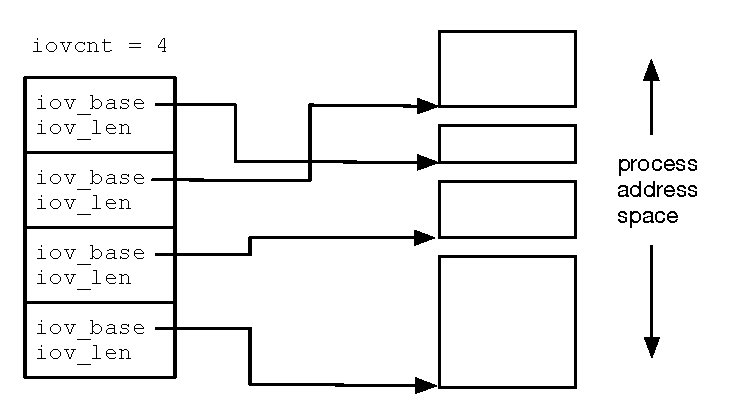
\includegraphics[scale=0.6]{figures/readv.pdf}
	\centering
	\caption{Issues multiple I/Os in a single system call using \cf{readv(2)} / \cf{writev(2)}}
	\label{fig:readv}
\end{figure}

Here are the functions that are available to perform vectored I/O. All are described by the \cf{readv(2)} manpage. The first two functions read / write from the current offset within the file. In figure \ref{fig:readv} there are four I/Os to different locations in memory but the data must be consecutive on disk.

\begin{lstlisting}
#include <sys/uio.h>

ssize_t readv(int fd, const struct iovec *iov, int iovcnt);
ssize_t writev(int fd, const struct iovec *iov, int iovcnt);

ssize_t preadv(int fd, const struct iovec *iov, int iovcnt,
               off_t offset);
ssize_t pwritev(int fd, const struct iovec *iov, int iovcnt,
                off_t offset);

ssize_t preadv2(int fd, const struct iovec *iov, int iovcnt,
                off_t offset, int flags);
ssize_t pwritev2(int fd, const struct iovec *iov, int iovcnt,
                 off_t offset, int flags);
\end{lstlisting}

\noindent
The \cf{preadv()} and \cf{pwritev()} functions combine reads/lseeks so that I/Os can take place from different offsets within the file as well as different areas in memory.

There are two main advantages of vectored I/O. The first is the reduction in the number of system calls that the application needs to make. Secondly if an application wishes to read data from a file into different locations in memory, using the \cf{read(2)} system call, the data would need to be read into a contiguous buffer in memory and then copied to the desired locations.

Here is an example of using both the \cf{readv()} and \cf{preadv()} functions in the same program. We start with a file of data that we're going to read which has ten \cf{0}s followed by ten \cf{1}s and so on:

\begin{lstlisting}
$ [*\bfseries cat vector-file*]
0000000000111111111122222222223333333333444444444455555555556666
666666777777777788888888889999999999
\end{lstlisting}

\noindent
The program source code is as follows:

\begin{lstlisting}
 1 #include <fcntl.h>
 2 #include <stdio.h>
 3 #include <unistd.h>
 4 #include <sys/uio.h>
 5  
 6 int
 7 main(int argc, char *argv[])
 8 {
 9     int  fd;
10     char buf2[32];
11     char buf3[32];
12     char buf1[32];
13     struct iovec bufs[] = {
14         { .iov_base = (void *)buf1, .iov_len = 10 },
15         { .iov_base = (void *)buf2, .iov_len = 10 },
16         { .iov_base = (void *)buf3, .iov_len = 10 },
17     };
18  
19     fd = open("vector-file", O_RDONLY);
20     lseek(fd, 10, SEEK_SET);
21     readv(fd, bufs, sizeof(bufs) / sizeof(bufs[0]));
22     printf("buf1 = %.10s\n", buf1);
23     printf("buf2 = %.10s\n", buf2);
24     printf("buf3 = %.10s\n", buf3);
25  
26     preadv(fd, bufs, sizeof(bufs) / sizeof(bufs[0]), 20);
27     printf("buf1 = %.10s\n", buf1);
28     printf("buf2 = %.10s\n", buf2);
29     printf("buf3 = %.10s\n", buf3);
30 }
\end{lstlisting}

\noindent
Here are the main points to discuss for this program:

\begin{itemize}
	\item line 10 - 12 -- we're allocating the buffers to read in to from the stack. But note that they'd been
		switched around so that they're not contiguous. Any order would work just the same.
	\item line 13 - 17 -- here are the definition of the \cf{iovec} structures to be used. There will be 3 reads of 10 bytes each.
	\item line 19 -- the file is opened read-only.
	\item line 20 -- a call is made to \cf{lseek(2)} to seek to byte 10 so the \cf{0}s will be skipped.
	\item line 21 -- the I/O call is issued.
	\item line 22 - 24 -- the first ten characters of each buffer is printed.
	\item line 26 -- this time the \cf{preadv(2)} system call is called. Prior to this call the file offset was changed to 40 following
		the call to \cf{readv(2)}. This time, we want to read starting at offset \cf{20}.
	\item line 27 - 29 -- print out ten characters from each buffer again.
\end{itemize}

\noindent
Here is the output when running the program:

\begin{lstlisting}
buf1 = 1111111111
buf2 = 2222222222
buf3 = 3333333333
buf1 = 2222222222
buf2 = 3333333333
buf3 = 4444444444
\end{lstlisting}

\noindent
Vectored I/O became popular with databases where large amount of I/O were needed but to different locations in memory where the database cached data. The basic interfaces were enhanced to allow different offsets in the file for each I/O. File I/O was later enhanced to avoid kernel caching (direct I/O) followed by backgrounding multiple I/Os, all to improve performance. Direct I/O and Async I/O will be described later in the chapter. 

%%%%%%%%%%%%%%%%%%%%%%%%%%%%%%%%%%%%%%%%%%%%%%%%%%%%%%%%%%%%%%%

\section{File and Record Locking}\label{prog-locking}

In a single application, a file can be accessed by multiple processes or by multiple threads within a single process. To handle synchronization between threads in a single processes there are various locking primitives that can be used by threads within the process. If multiple processes are accessing a file simultaneously, there are a different set of file and record locking interfaces that can be used to coordinate access. Historically, file locking has been a bit of a mess.

Some of these interfaces predate per-process multi-threading support. In particular, \textit{ddvisory} and \textit{mandatory} file locking have been around for many years and come with a set of issues that developers should be aware of. 

%------------------------------------------------------------------------------------------------------------------------------------------------------------

\subsection{Advisory File Locking}

The first type of file locking introduced in UNIX and available in Linux, was \textit{advisory locking} also called record locking since byte ranges within a file can be locked but processes must query to determine what portions of the file are locked. Thus the "advisory" part of the implementation.

To make things confusing, there are three functions that can be used for advisory locking namely \cf{fcntl(2)}, \cf{lockf(3)} and \cf{flock(2)}. On Linux, \cf{lockf(3)} is simply implemented on top of \cf{fcntl(2)} and any locks implemented through use of \cf{fnctl(2)} are ignored.

To get started, here is the interface for \cf{fcntl(2)}:

\begin{lstlisting}
#include <fcntl.h>

int fcntl(int fd, int cmd, ... /* arg */ );
\end{lstlisting}

\noindent
The \cf{cmd} argument will be \cf{F\_SET\_LK},  \cf{F\_SETLKW} or \cf{F\_GETLK} dependent on whether the caller wants to acquire, release or test for the existence of a record lock. The third argument passed is a pointer to an \cf{flock} structure which specifies what part of the file should be locked:
\begin{lstlisting}
struct flock {
   ... 
   short l_type;    /* Lock type: F_RDLCK, F_WRLCK, F_UNLCK */
   short l_whence;  /* How to interpret l_start. One of:
                           SEEK_SET, SEEK_CUR, SEEK_END */
   off_t l_start;   /* Starting offset for lock */
   off_t l_len;     /* Number of bytes to lock */
   pid_t l_pid;     /* PID of process blocking our lock
                       (set by F_GETLK and F_OFD_GETLK) */
   ... 
}; 
\end{lstlisting}

\noindent
The \cf{l\_type} field specifies whether the caller wants to take a read lock, a write lock or just unlock a previously locked set of bytes. The \cf{l\_whence},  \cf{l\_start} and \cf{l\_len} fields of this structure specify the range of bytes that the caller wishes to lock.

There is some deadlock detection built into the implementation such that if two processes attempt to access a region of the file that is locked by the other process, an \cf{EDEADLK} error will be returned and thus the caller should release some of its locks allowing others to proceed.

The implementation of this style of locking has other issues which will be described in section \ref{linux-adv-locking}.

%------------------------------------------------------------------------------------------------------------------------------------------------------------

\subsection{An Example of Advisory Locking}

This section shows two programs that work together to show how advisory locking can work between two processes. The first program (\cf{alock}) takes a write lock on the file "\cf{hello}" and over the whole file. It waits until it receives a signal (\cf{SIGUSR1} before releasing the lock.

The second program (\cf{lcat} calls the \cf{system(3)} library function to \cf{cat} the contents of the file. Before doing so, it checks three times to see if the file is locked. If it's still locked after the third check, it sends \cf{SIGUSR1} to the process that holds the lock. It can then display the file.

Here is the \cf{alock.c} program:

\begin{lstlisting}
 1 #include <unistd.h>
 2 #include <fcntl.h>
 3 #include <signal.h>
 4 #include <stdio.h>
 5 
 6 void
 7 mysig_hdlr(int signo)
 8 {
 9     printf("alock - got signal\n");
10     return;
11 }
12 
13 int
14 main()
15 {
16     struct flock     lock;
17     int              fd;
18     struct sigaction action;
19 
20     action.sa_handler = mysig_hdlr;
21     sigemptyset(&action.sa_mask);
22     action.sa_flags = 0;
23     sigaction(SIGUSR1, &action, NULL);
24 
25     fd = open("hello", O_RDWR);
26 
27     lock.l_type = F_WRLCK;
28     lock.l_whence = SEEK_SET;
29     lock.l_start = 0;
30     lock.l_len = 0;
31     lock.l_pid = getpid();
32     fcntl(fd, F_SETLK, &lock);
33     
34     printf("alock - file now locked\n");
35     pause();
36     lock.l_type = F_UNLCK;
37     fcntl(fd, F_SETLK, &lock);
38     printf("alock - file now unlocked\n");
39 }
\end{lstlisting}

\noindent
Some comments on the code:

\begin{itemize}
	\item lines 20 - 23 -- set up a signal handler (\cf{mysig\_hdlr}) for \cf{SIGUSR1}.
	\item lines 27 - 32 -- set a write lock on the file for the whole file by setting \cf{l\_start} to \cf{0} and \cf{l\_len} to \cf{0}. 
	\item line 35 -- pause waiting for \cf{SIGUSR1}.
	\item lines 36 - 37 -- release the lock (keeping the original fields that specify the start/length which is the whole file).
\end{itemize}

\noindent
Here is the source code for the \cf{lcat.c} program:

\begin{lstlisting}
 1 #include <signal.h>
 2 #include <stdlib.h>
 3 #include <unistd.h>
 4 #include <fcntl.h>
 5 #include <stdio.h>
 6 
 7 pid_t
 8 file_is_locked(int fd)
 9 {
10     struct flock    lock;
11 
12     lock.l_type = F_RDLCK;
13     lock.l_whence = SEEK_SET;
14     lock.l_start = 0;
15     lock.l_len = 0;
16     lock.l_pid = 0;
17 
18     fcntl(fd, F_GETLK, &lock);
19     return (lock.l_type == F_UNLCK) ? 0 : lock.l_pid;
20 }
21 
22 int main()
23 {
24     pid_t  pid;
25     int    i, fd;
26 
27     fd = open("hello", O_RDONLY);
28 
29     for (i = 0 ; i < 3 ; i++) {
30         if ((pid = file_is_locked(fd)) != 0) {
31             printf("lcat - waiting for lock\n");
32             sleep(1);
33         } else {
34             system("cat hello"); /* shouldn't get here */
35         }
36     }
37     printf("pid = %d\n", pid);
38     kill(pid, SIGUSR1);
39     sleep(1);
40     if ((pid = file_is_locked(fd)) == 0) {
41         system("cat hello");
42     } else {
43         /* shouldn't get here */
44         printf("lcat - lock still not released\n");
45     }
46 }
\end{lstlisting}

\noindent
Some comments on the code:

\begin{itemize}
	\item lines 10 - 19 -- the \cf{file\_is\_locked()} function checks to see if this process can take a read lock over
		the whole file. If it can it returns 0 and if it can't it returns the PID of the process that holds a lock that covers
		this range.
	\item lines 29 - 34 --  this program loops three times checking to see if the read lock can be taken. There is 
		nothing special about this loop. The idea is just that if the lock can't be taken, the program could be doing
		something else. After the 3rd attempt, it drops out with the PID of the process that holds the lock.
	\item line 38 - 39 -- send SIGUSR1 to the process that holds the lock. The \cf{alock} process will catch the signal
		and release the lock. It then waits a second to give \cf{alock} time to process the signal and unlock the file.
	\item lines 40 - 41 -- another check is made to see if \cf{lcat} can get the read lock. If it can, it will \cf{cat}
		the contents of the file.
\end{itemize}

\noindent
There are two places in the program where it states that the code path should not get there. This is certainly the case if only these two processes are accessing the file. If there are others, this could change. On line 43, this path could be reached if the "1" second sleep isn't enough to allow \cf{alock} to unlock the file.

Here are the two programs running in separate terminals but with the output merged so you can see the order of events:

\begin{lstlisting}
$ [*\bfseries ./alock*]                  |   
alock - file now locked    | 
                           | $ [*\bfseries ./lcat*]
                           | lcat - waiting for lock 
                           | lcat - waiting for lock 
                           | lcat - waiting for lock 
alock - got signal         | 
alock - file now unlocked  | 
                           | pid = 9671
                           | Hello world!
\end{lstlisting}

\noindent
Since this is advisory locking, applications must work in coordination with each other and non-cooperating applications cannit interfere otherwise assumptions will be broken. It would be best to segregate these applications and files so that no other users/processes can get access to them.

%------------------------------------------------------------------------------------------------------------------------------------------------------------

\subsection{Viewing Existing Locks}

Existing locks currently in use can be view in two ways. The first is to use the \cf{lslocks(1)} command:

\begin{lstlisting}
$ [*\bfseries lslocks -b*]
COMMAND     PID  TYPE  SIZE MODE  M START END PATH
multipathd  441  POSIX      WRITE 0     0   0 /run/snapd/ns...
cron        838  FLOCK      WRITE 0     0   0 /run/snapd/ns...
snapd       653  FLOCK      WRITE 0     0   0 /...
alock     10397  POSIX  13  WRITE 0     0   0 /home/.../hello
\end{lstlisting}

\noindent
In the last line you can see the \cf{alock} process that holds the \cf{WRITE} lock for \cf{13} bytes which is the length of the file. The type of lock depends on the call made. POSIX locks are created using the lockf(2) or \cf{fcntl(2)} system calls and FLOCK locks are created using the \cf{flock(2)} system call. 

The second method is to view the locks through \cf{/proc} as follows:

\begin{lstlisting}
$ [*\bfseries cat /proc/locks*]
1: POSIX  ADVISORY  WRITE 10397 fd:00:396261 0 EOF
2: FLOCK  ADVISORY  WRITE 653 fd:00:528747 0 EOF
3: FLOCK  ADVISORY  WRITE 838 00:1b:1248 0 EOF
4: POSIX  ADVISORY  WRITE 441 00:1b:506 0 EOF
$ [*\bfseries ps -ef | grep 10397*]
spate      10397    4862  0 23:35 pts/1    00:00:00 ./alock
\end{lstlisting}

\noindent
The obvious difference here is that there the command name is not shown although the process ID is displayed and can be easily used to find the process.

%------------------------------------------------------------------------------------------------------------------------------------------------------------

\subsection{Mandatory File Locking}

Since not all processes check for file locks, it was deemed that advisory locking needed a fix. The solution was the introduction of \textit{mandatory file locking} in SVR3 UNIX whereby access to a file would be denied if it was locked regardless of whether a process checks for locks or not. The intention of the scheme was to have as little impact as possible on existing applications. Of course, applications needed to be aware about how to handle the denial case. And to make matters worse, system calls such as \cf{unlink(2)} were able to succeed.

To enable mandatory file locking in Linux there are two steps that are needed:

\begin{enumerate}
	\item The underlying file system must be mounted with the \cf{mand} option (for example "\cf{mount -o mand -t 
		spfs /dev/sdb1 /mnt}").
	\item For the file to be locked, the set-group-ID bit must be turned on and the group-execute bit must be turned off for all
		files that need to be locked (for example "\cf{chmod g+s,g-x <file>}"). This is a combination that otherwise makes
		no sense. You can't get an uglier solution than this!
\end{enumerate}

\noindent
After a process places a mandatory lock on a file, no other process can access the file for reading or writing. 

As the \cf{Documentation/filesystems/mandatory-locking.txt} file in the kernel source tree indicates, there are several problems with mandatory locking. Firstly, "\textit{the write system call checks for a mandatory lock only once at its start.  It is therefore possible for a lock request to be granted after this check but before the data is modified. A process may then see file data change even while a mandatory lock was held."} There are also problems with \cf{read(2)} and \cf{mmap(2)}. Please consult this document if you have further interest in the issues surrounding mandatory file locking.

In Linux it's very clear that there is no love for mandatory locking and there have been attempts to remove it for many years. The "\textit{no regressions}" rule such that APIs cannot be removed in case it breaks an old application have resulted in the code still being there even though it's unknown whether anything still used mandatory locks.

As such, no further time will be given to mandatory locking.

%------------------------------------------------------------------------------------------------------------------------------------------------------------

\subsection{Open File Description Locks}\label{linux-adv-locking}

Linux introduced file-private POSIX locks in the 3.x kernel series with the goal of taking elements of both BSD-style and POSIX-style locks and combining them into a more robust locking API by removing some of the ambiguity that existed across the various UNIX platforms. The following article describes the work that was done and covers some of the problems that were solved. It also provides an example of using open file description locks in a multi-threaded environment. This section will highlight those changes.

\begin{table}[h]
\begin{tabular}{lcl}
\parbox[r]{0.5in}{
\includegraphics[scale=0.15]{figures/url.png}} & \parbox[l]{0.55in}{URL \arabic{urls}} & \parbox[l]{3in}{\cf{https://lwn.net/Articles/586904/}}
\end{tabular}
\end{table}
\stepcounter{urls}
% https://lwn.net/Articles/586904/

\noindent
One specific problem with POSIX locks is that when a request for a lock is made that would conflict with an existing lock previously taken by the same process, the kernel treats it as a request to modify the existing lock. This makes POSIX locks as good as useless in a multi-threaded application. 

If a process closes a file then all locks will be released even if a lock was taking using a different file descriptor (see \cf{dup(2)} and friends). Also, as the above article states "\textit{This is a particular problem for applications that use complex libraries that do file access. It's common to have a library routine that opens a file, reads or writes to it, and then closes it again, without the calling application ever being aware that has occurred. If the application happens to be holding a lock on the file when that occurs, it can lose that lock without ever being aware of it. That sort of behavior can lead to silent data corruption, and loss of developer sanity.}". This could be, and has been, a very difficult problem to debug.

In general, if you need to use advisory locking, use the newer Open File Description Locks and avoid using POSIX-style locking.

%%%%%%%%%%%%%%%%%%%%%%%%%%%%%%%%%%%%%%%%%%%%%%%%%%%%%%%%%%%%%%%

\section{Synchronizing I/O Operations}

Generally speaking, when data is written to a file, it is not automatically written to disk but written to the page cache that resides in the Linux kernel address space. Modified data will eventually be written to disk. Obviously this presents an issue if the system were to crash prior to this data being written. The same is true of the file's metadata which could include the file size.

There are two system calls that allow for flushing modified data and metadata that may be sitting in kernel caches that have not yet made it to disk. Both are described in the \cf{fsync(2)} manpage:

\begin{lstlisting}
#include <unistd.h>

int fsync(int fd);
int fdatasync(int fd);
\end{lstlisting}

\noindent
The \cf{fsync(2)} system call will flush any modified data that is still in memory. This includes any file data as well as file metadata (file attributes). This ensures that the changes will make it to disk such that if the system crashes, any data can still be retrieved.

The  \cf{fdatasync(2)} system call is similar but does not flush metadata. 

%%%%%%%%%%%%%%%%%%%%%%%%%%%%%%%%%%%%%%%%%%%%%%%%%%%%%%%%%%%%%%%

\section{Direct I/O}

% https://www.scylladb.com/2017/10/05/io-access-methods-scylla/ - good article

When file I/O occurs, data is cached in the kernel inside the \textit{page cache}. If data read or written is in the page cache it can be accessed without additional I/Os. This type of I/O is also called \textit{buffered I/O} since the data is \textit{buffered} in the kernel. Traditionally it was cached in the \textit{buffer cache}. 

Not all applications want data to be cached since they can better manage that cache themselves. The typical example is that of databases which allocate very large caches in the user address space.

Figure \ref{fig:direct-io} shows the three different paths that I/O can take. There are subtle differences between buffered I/O and mapped I/O.

\begin{figure}
	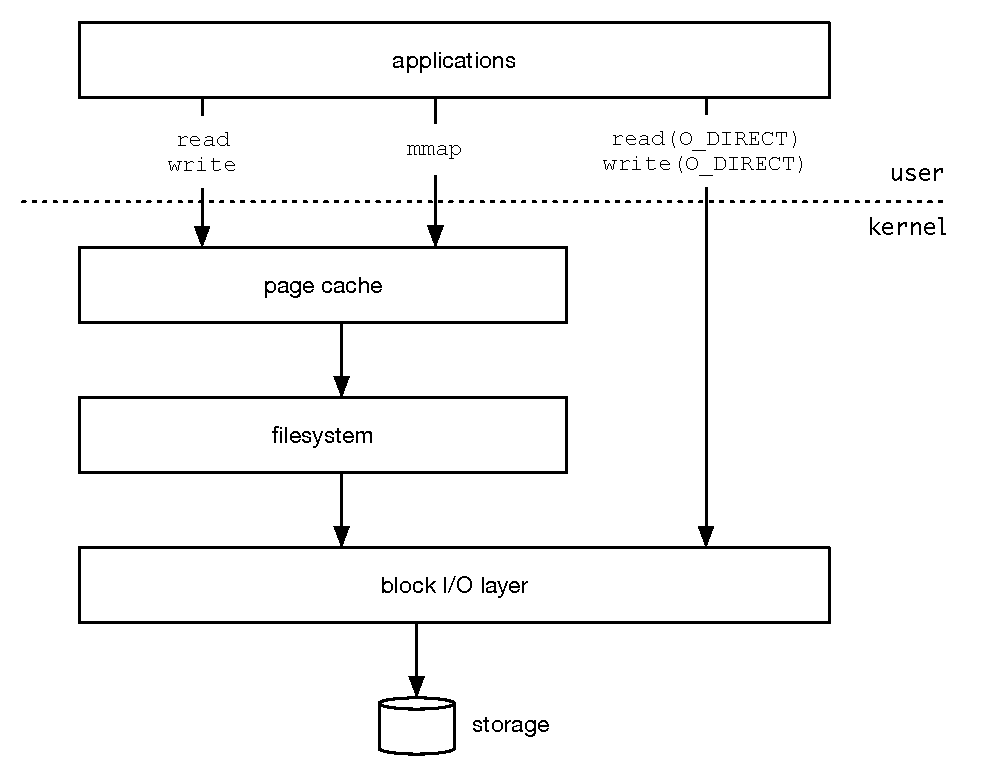
\includegraphics[scale=0.6]{figures/direct-io.pdf}
	\centering
	\caption{There are 3 paths to disk from applications}
	\label{fig:direct-io}
\end{figure}

\begin{enumerate}
	\item \textbf{Buffered I/O} -- this is the default type of I/O. Access goes through the filesystem and data is cached in
		the page cache. Strictly speaking, for writes, the data is written into page cache pages and at a later data, a call
		is made into the filesystem to flush them to disk. For reads, pages are allocated and a call is made into the 
		filesystem to read data from disk.
	\item \textbf{Memory mapping} -- applications access files through mappings into their address space. When data needs
		to be read or written, the kernel calls into the filesystem to perform the I/O. Once a page is in memory it will
		continue to be accessed through the mapping until a later date when data is flushed or the mapping is destroyed.
	\item \textbf{Direct I/O} -- the page cache is bypassed and data transfers directly between the process address space
		and disk.
\end{enumerate}

\noindent
Applications can request direct I/O by passing the \cf{O\_DIRECT} flag to the \cf{open(2)} system call. To enable direct I/O applications must be compiled with \cf{\_ALL\_SOURCE} enabled to see the definition of \cf{O\_DIRECT}.

The performance gains due to direct I/O are very dependent on the application's ability to effectively manage its own cache of data. There may be additional complexities if a file is being accessed through a mix of buffered I/O and direct I/O, certainly a situation that should be avoided.

Once a file is opened, reads and writes proceed as normal with the exception of alignment of user addresses and the amount of I/O requested. These restrictions are per-filesystem and there is no generic way in which to determine what the constraints imposed are.

\begin{itemize}
	\item The number of bytes to be transferred is a multiple of 512 bytes.
	\item The file offset is a multiple of 512 bytes.
	\item The user-supplied memory address is aligned on a 512-byte boundary.
\end{itemize}

\noindent
Note that some filesystems may have different requirements. For example, VxFS only requires a 8-byte boundary for the user address. XFS has the \cf{XFS\_IOC\_DIOINFO} command that can be passed to \cf{xfsctl(3)} to determine requirements.

There is no easy way to show direct I/O in progress or when it works or doesn't work. However, section \ref{kernel-direct-io} will describe the implementation of direct I/O and gives examples to show that the page cache is in fact bypassed.

%%%%%%%%%%%%%%%%%%%%%%%%%%%%%%%%%%%%%%%%%%%%%%%%%%%%%%%%%%%%

\section{Sparse Files}

A sparse file is a regular file that has one or more \textit{holes}. If you're not familiar with sparse files, that's going to sound like a very strange statement. Another way to put it is that a sparse file is a file that allows for efficient storage allocation for large amounts of data. If you've used virtual machines at any point in time, they're underpinned by sparse files. For example, consider a VM that has a 60 GB disk. When the VM is created, it doesn't need this much space and likely to be a small fraction. So why allocated 60 GB of disk space if it's not needed? This becomes a bigger problem as more and more VMs are created on the same storage infrastructure.

Sparse files are also useful when large parts of the file contain zeros. This avoids all data blocks being allocated up front. When data is written over a hole, new blocks will be allocated.

Sparse files can be found using the \cf{find(1)} command. For example, looking inside \cf{/var/log}, there are two sparse files:

\begin{lstlisting}
$ [*\bfseries sudo find /var/log -type f -printf "\%S\textbackslash t\%p\textbackslash n" | \textbackslash*]
  [*\bfseries gawk '\$1 < 1.0 {print}'*]
0.013824	/var/log/lastlog
0.127872	/var/log/faillog
\end{lstlisting}

\noindent
Selecting one of these files, \cf{ls(1)} can be used to view the file size and the number of blocks backing the file:

\begin{lstlisting}
$ [*\bfseries ls -lh /var/log/lastlog*]
-rw-rw-r-- 1 root utmp 290K Aug  1 17:16 /var/log/lastlog
$ [*\bfseries du -sh /var/log/lastlog*]
4.0K	/var/log/lastlog
\end{lstlisting}

\noindent
There is only 4 KB allocated to the file but the file size is 290 KB.

%------------------------------------------------------------------------------------------------------------------------------------------------------------------

\subsection{Sparse Files in Action}

Let's demonstrating with a small program which opens/creates a file, writes "\cf{hello}" at offset 0 then seeks to an offset of 16 KB and writes "\cf{world}". We're going to have to explore some details inside the filesystem to explain what's happening.

\begin{lstlisting}
#include <stdio.h>
#include <string.h>
#include <errno.h>
#include <unistd.h>
#include <fcntl.h>

char *buf1 = "hello";
char *buf2 = "world";

int
main(int argc, char *argv[])
{
    int fd = open("/mnt/foo", O_CREAT|O_WRONLY, 0700);
    write(fd, buf1, strlen(buf1));
    lseek(fd, 16384, SEEK_SET);
    write(fd, buf2, strlen(buf2));
}
\end{lstlisting}

\noindent
Now let's look at the file:

\begin{lstlisting}
# [*\bfseries ls -l /mnt/foo*]
-rwx------ 1 root root 16389 Dec 15 20:54 /mnt/foo
\end{lstlisting}

\noindent
This is the expected size of the file but what's after "\cf{hello}" and before we get to "\cf{world}" at an offset of 16384? The answer isn't always consistent and depends on the underlying filesystem and its properties. But to give one example and where a file is sparse, we've created this file on top of SPFS, the disk-based filesystem whose implementation will be described in chapter \ref{disk-fs}.

This particular filesystem has a block size of 2048 bytes. This is the minimum amount of space that can be allocated to any file. Ignoring our sparse file example, if we were to start writing sequentially to a file at 0, SPFS would allocate blocks to the file as follows:

\begin{itemize}
	\item bytes 0 - 2047 --- allocate block
	\item bytes 2048 - 4195 --- allocate block
	\item bytes 4196 - 6143 --- allocate block
	\item and so on
\end{itemize}

\noindent
If we only wrote 1 byte at offset 0, we'd get 1 block allocated. If we wrote 2048 bytes at offset 0 (for a total of 2049 bytes), we'd get two blocks allocated and so on.

Let's take a look at the file using the \cf{stat(1)} command:

\begin{lstlisting}
# [*\bfseries stat /mnt/foo*]
  File: /mnt/foo
  Size: 16389     	  [*\bfseries Blocks: 2*] IO Block: 2048 regular file
Device: 800h/2048d	  Inode: 4  Links: 1
Access: (0700/-rwx------) Uid: ( 0/  root)   Gid: ( 0/  root)
Access: 2022-12-15 20:54:09.000000000 +0000
Modify: 2022-12-15 20:54:09.000000000 +0000
Change: 2022-12-15 20:54:09.000000000 +0000
\end{lstlisting}

\noindent
There are 2 blocks allocated to this file as highlighted. Each block is 2048 bytes so that's a total of 4096 bytes. But our file is now 16389 bytes according to \cf{ls(1)}. Both are correct. The file is sparse so has a hole in the middle. Next, we are going to use the SPFS filesystem debugger and display the contents of the inode for the file that we've written. We'll cover inodes in detail later but just think of it as a filesystem structure that records information about a file. You can see the file size and also see that a block (131) has been allocated for block offset 0 and another block (132) has been allocated at block offset 8. There are no allocated blocks for block offsets 1 through 7.

\begin{lstlisting}
spfsdb > [*\bfseries i4*]
inode number 4
  i_mode     = 81c0
  i_nlink    = 1
  i_atime    = Thu Dec 15 20:54:09 2022
  i_mtime    = Thu Dec 15 20:54:09 2022
  i_ctime    = Thu Dec 15 20:54:09 2022
  i_uid      = 0
  i_gid      = 0
  i_size     = 16389
  [*\bfseries i\_blocks   = 2*]
  [*\bfseries i\_addr[ 0] = 131   i\_addr[ 8] = 132*]
\end{lstlisting}

\noindent
The layout of the file is shown pictorially in figure \ref{fig:sparse}. If the application were to read the file, it would see "\cf{hello}" followed by a lot of zeroes followed by "\cf{world}".

\begin{figure}
	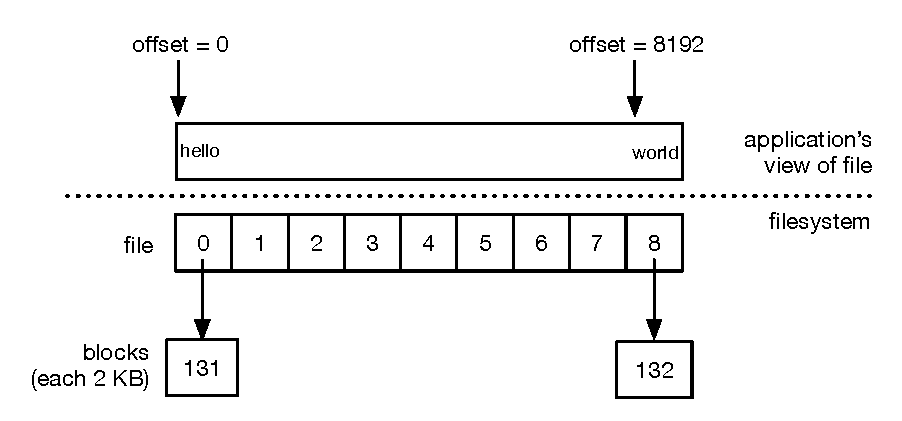
\includegraphics[scale=0.6]{figures/sparse.pdf}
	\centering
	\caption{A sparse file only showing 2 allocated blocks}
	\label{fig:sparse}
\end{figure}

In fact, this doesn't work - \textbf{XXX---bug - see notes. Needs fixing}

\subsection{Sparse File Example 1 --- Virtual Machines}

Virtual Machines are a wonderful application of how sparse files achieve the goal of mimicking large devices but only allocate data as and when needed. Disks are generally represented as sparse files in some underlying filesystem that is storing the virtual disks. When you create a virtual disk, under the covers, the hypervisor creates a sparse file on disk in a similar way to our simple program above. As the VM operating system writes blocks to disk, the hypervisor translates these writes into lseek/write combinations. Over time, you end up with a sparse file that has many holes and an ever increasing amount of allocated storage as the VM writes more and more data

In commercial implementations with 100s or 1000s of VMs, the cost savings can be huge. Storage does not need to all be allocated up front and can be added later as VM disks start to grow. Furthermore, data deduplication is typically deployed. 100s of VMs have a very similar footprint in terms of operating system binaries and such like.

%------------------------------------------------------------------------------------------------------------------------------------------------------------------

\subsection{Sparse File Example 2 --- HSM Applications}

An older but very relevant example of how sparse files were used by applications was for HSM (Hierarchal Storage Management) applications. There was a whole standard developed around this called DMIG (Data Management Interfaces Group). When I was at SCO, I used to travel from the UK to the US every 6 weeks or so to attend meetings. I got to visit several new cities and meet a lot of prominent operating system and filesystem engineers from the top companies at the time.

In the early 90s, disks were much smaller than you see today and also very expensive. Therefore to save space, several vendors developed what were then called HSM applications. The goal of such applications was to run periodically and perform the following:

\begin{itemize}
	\item Look for files that have not recently been accessed.
	\item Migrate the \textit{punched data} off to tape or other cheap storage.
	\item Punch a hole in the file. More likely, the hole would be from a specific offset to the end of the file.
	\item Make sure that the timestamps were not modified.
\end{itemize}

\noindent
A small amount of data was left at the start of each \textit{managed file} to satisfy requested from commands such as \cf{file(1)} which would read from the start of the file to determine file type. If a request was made to read/write to a portion of the file that had been migrated, the application would be paused while the data was read from tape and written back to the file.

Sound complicated? Yes it was and was made even more complicated by the fact that there was a lot of hacking of existing filesystems and parts of the kernel to make this work across different operating systems. And with several commercial versions of UNIX at the time, porting HSM applications was prohibitive. 

But this was a big enough problem and there was enough customer demand that the DMIG standard was developed and published and many operating system and filesystem vendors implemented support. Move forward twenty years and there is little information on the web now. In fact a Google search while writing this showed a fragment from my previous book on UNIX Filesystems but little else.

%%%%%%%%%%%%%%%%%%%%%%%%%%%%%%%%%%%%%%%%%%%%%%%%%%%%%%%%%%%%%%%

\section{Buffered I/O and the Standard I/O Library}\label{stdio}

We covered the \cf{read(2)} and \cf{write(2)} system calls earlier and other sections in this chapter cover specialized I/O capabilities such as vectored reads/writes and asynchronous I/O. This section describes how the standard I/O library operates.

As the \cf{stdio(3)} man page says:

\begin{quote}
\textit{The  standard  I/O  library  provides  a  simple and efficient buffered stream I/O interface.  Input and output is  mapped  into  logical  data streams  and the physical I/O characteristics are concealed.}
\end{quote}

\noindent
Figure \ref{fig:stdio-1} shows the position of the standard I/O library in relation to an application and the Linux kernel. Developers have two choices when operating on a file. They can use system calls directly or they can use the standard I/O library which contains a wide array of functions for dealing with file I/O. The \cf{stdio(3)} manpage provides a good overview of the standard I/O library and the functions that it provides. There are approximately 56 different functions available. All C developers will be familiar with the \cf{printf(3)} function including their first "\textit{Hello world}" program. Well, \cf{printf(3)} is one of the 56 functions and by default, it writes to the standard output file stream.

\begin{figure}
	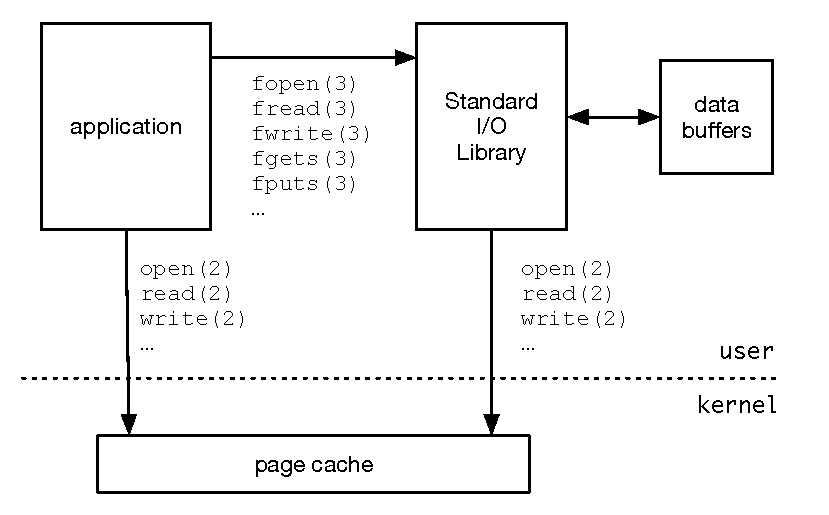
\includegraphics[scale=0.6]{figures/stdio-1.pdf}
	\centering
	\caption{Using the Standard Library vs System Calls}
	\label{fig:stdio-1}
\end{figure}

Whether to use system calls directly or use the standard library is very dependent on what your application does. If you are developing an application that processes text files, the standard library is generally the better choice. You can read/write single characters at a time, read lines terminated by newlines or format the data then write to a file stream. For the standard I/O library, \cf{printf(3)} and friends ease the job of formatting text to be written. The same is true for \cf{scanf(3)} and similar functions. If you use the system calls \cf{read(2)} and \cf{write(2)} and want to process text, you'll likely repeat the work that the standard I/O library has already done for you.

%------------------------------------------------------------------------------------------------------------------------------------------------------------------

\subsection{The Standard I/O Library \cf{FILE} Structure}

Let's take a look at a few functions provided by the standard I/O library. In all cases the \cf{stdio.h} header file needs to be included.

\begin{lstlisting}
#include <stdio.h>

FILE *[*\bfseries fopen*](const char * restrict path,
            const char * restrict mode);
int [*\bfseries fclose*](FILE *stream);
size_t [*\bfseries fread*](void *restrict ptr, size_t size,
             size_t nitems, FILE *restrict stream);
int [*\bfseries fscanf*](FILE *restrict stream, 
           const char *restrict format, ...);
\end{lstlisting}

\noindent
The standard library operates on a \textit{file stream} as defined by the \cf{FILE} structure. The \cf{stdio.h} header file doesn't contain the definition of \cf{struct FILE}. For that you need to look at the following header file:

\begin{lstlisting}
/usr/include/aarch64-linux-gnu/bits/types/FILE.h
typedef struct _IO_FILE FILE;
\end{lstlisting}

\noindent
which is part of the glibc source repository. To get to "\cf{struct \_IO\_FILE}" you need to look in the glibc sources:

\begin{itemize}
	\item In the glibc source code
	\subitem \cf{glibc/libio/bits/types/struct\_FILE.h}
    	\item On my Ubuntu VM under \cf{/usr/include}
	\subitem \cf{aarch64-linux-gnu/bits/types/struct\_FILE.h}  
\end{itemize}

\noindent
Here is part of the structure, specifically those fields that we'll be covering in this section to help understand how buffered I/O works:

\begin{lstlisting}
struct _IO_FILE
{
  int                _flags;     
  char              *_IO_read_ptr;
  char              *_IO_read_end;  
  char              *_IO_read_base;  
  char              *_IO_write_base; 
  char              *_IO_write_ptr; 
  char              *_IO_write_end;  
  char              *_IO_buf_base;
  char              *_IO_buf_end;  
  char              *_IO_save_base;
  char              *_IO_backup_base;  
  char              *_IO_save_end; 
  struct _IO_marker *_markers;
  struct _IO_FILE   *_chain;
  int                _fileno;
  int                _flags2;
  unsigned short     _cur_column;
  signed char        _vtable_offset;
  char               _shortbuf[1];
  _IO_lock_t        *_lock;
};
\end{lstlisting}

\noindent
One of the best ways to view what is happening when you use the standard I/O library is run a simple program under \cf{gdb}, set breakpoints and view the different fields in the \cf{FILE} structure. Here is a very simple program which will be used to demonstrate this point:

\begin{lstlisting}
 1  #include <stdio.h>
 2
 3  int
 4  main()
 5  {  
 6      FILE *fp;
 7      int         c; 
 8
 9      fp = fopen("lorem-ipsum", "r");
10      c = fgetc(fp);
11      printf("char = %c\n", (char)c);
12  }  
\end{lstlisting}

\noindent
The "\cf{lorem-ipsum}" file contains the commonly seen Latin text starting "\cf{Lorem ipsum dolor sit ...}" which is used throughout the book. In case you've ever wondered where this text came from, Wikipedia informs us that:

\begin{quote}
\textit{Lorem ipsum is typically a corrupted version of De finibus bonorum et malorum, a 1st-century BC text by the Roman statesman and philosopher Cicero, with words altered, added, and removed to make it nonsensical and improper Latin.}
\end{quote}

\noindent
In our \cf{gdb} session, we'll set a breakpoint, run the program and display the character read ("\cf{L}" as expected) as well as the contents of the \cf{FILE} structure:

\begin{lstlisting}
(gdb) [*\bfseries b 11*]
Breakpoint 1 at 0x840: file fget.c, line 11.
(gdb) [*\bfseries run*]
Starting program: /home/spate/spfs/test/fget 
[Thread debugging using libthread_db enabled]
Using host libthread_db library "/lib/aarch64-linux-gnu...
	
Breakpoint 1, main () at fget.c:11
11		printf("char = [*\%c\textbackslash*]n", (char)c);
(gdb) [*\bfseries p c*]
$1 = 76
(gdb) [*\bfseries p (char)c*]
$2 = 76 'L'
(gdb) [*\bfseries p *fp*]
$3 = {_flags = -72539000, 
  _IO_read_ptr = 0xaaaaaaac1481 "orem ipsum dolor sit amet"..., 
  _IO_read_end = 0xaaaaaaac201c "", 
  _IO_read_base = 0xaaaaaaac1480 "Lorem ipsum dolor sit"..., 
  _IO_write_ptr = 0xaaaaaaac1480 "Lorem ipsum dolor sit"..., 
  _IO_buf_base = 0xaaaaaaac1480 "Lorem ipsum dolor sit"..., 
  _IO_buf_end = 0xaaaaaaac2480 "", _IO_save_base = 0x0, 
  _IO_backup_base = 0x0, _IO_save_end = 0x0, _markers = 0x0, 
  _chain = 0xfffff7fa1520 <_IO_2_1_stderr_>, _fileno = 3, 
  _flags2 = 0, _old_offset = 0, _cur_column = 0, 
  _vtable_offset = 0 '\\000', _shortbuf = "",  
  _lock = 0xaaaaaaac1380, _offset = -1, _codecvt = 0x0, 
  _wide_data = 0xaaaaaaac1390, _freeres_list = 0x0, 
  _freeres_buf = 0x0,  __pad5 = 0, _mode = -1, 
  _unused2 = '\000' <repeats 19 times>}
\end{lstlisting}

\noindent
The \cf{\_fileno} field is the file descriptor referencing the open file. Since this is the only file used by the application other than the standard file descriptors, when the file is opened a file descriptor of 3 is returned.

The \cf{\_IO\_buf\_base} points to a a buffer in which data is read into and written from. The \cf{\_IO\_buf\_end} points to the end of the buffer so, in theory we have 4 KB of data that's been read from the file. But since the file is only 2,972 bytes in size we see that \cf{\_IO\_read\_end} is set to \cf{0x201c}. Subtracting the two we have \cf{0x201c – 0x1481 = 0xB9B} which in decimal is \cf{2971}. Since the first character of the file is stored at \cf{0x201c}, this makes \cf{2972}, the size of the file.

The \cf{\_IO\_read\_ptr} and \cf{\_IO\_write\_ptr} fields reference the position within this 4 KB buffer where we are currently reading and writing from/to. Since we've read a single character from the file, \cf{\_IO\_read\_ptr} is incremented to point to the next position in the buffer (the character "\cf{o}").

%------------------------------------------------------------------------------------------------------------------------------------------------------------------

\subsection{Analyzing the glibc Standard I/O Library}

You can download the most recent glibc source code as follows:

\begin{lstlisting}
# [*\bfseries git clone https://sourceware.org/git/glibc.git*]
# [*\bfseries cd glibc*]
# [*\bfseries git checkout master*]
\end{lstlisting}

\noindent
As an example of how to see what glibc is doing, navigate to the \cf{libio} directory and choose the field of the \cf{FILE} that you wish to analyze, for example:

\begin{lstlisting}
   # [*\bfseries grep \_IO\_read\_ptr *c*]
\end{lstlisting}

\noindent
You will see lots of references. To understand the flow through the library calls you'll need to spend some time analyzing the code. There are several indirections. For example, for \cf{fread(3)} start at \cf{\_IO\_fread()} in \cf{iofread.c} and go from there. You can also use the Elixir Cross Referencer, for example:

\begin{lstlisting}
https://elixir.bootlin.com/glibc/latest/source/libio/iofread.c
\end{lstlisting}

\noindent
I actually found it easier to grep. For example, search for the following:

\begin{lstlisting}
'fp->_IO_read_ptr'
'fp->_IO_read_ptr ='
[*\bfseries 'fp->\_IO\_read\_ptr+'*]
'fp->_IO_read_ptr-'
\end{lstlisting}

\noindent
and you'll see a smaller set of hits. For the highlighted option, there were only 3 hits:

\begin{lstlisting}
$ [*\bfseries grep 'fp->\_IO\_read\_ptr+' *c*]
genops.c:    return *(unsigned char *) fp->_IO_read_ptr++;
genops.c:	return *(unsigned char *) fp->_IO_read_ptr++;
genops.c:  return *(unsigned char *) fp->_IO_read_ptr++;
\end{lstlisting}

\noindent
Looking inside \cf{genops.c} in the function \cf{\_\_uflow()}, there is a fragment of code:

\begin{lstlisting}
if (fp->_IO_read_ptr < fp->_IO_read_end)
  return *(unsigned char *) fp->_IO_read_ptr++;
\end{lstlisting}

\noindent
A character is being returned from the current read pointer and the read pointer is being incremented as long as the read pointer still references data in the buffer (first line).

I started to experiment further by extending the program to do the following and printing out various pointers in the \cf{FILE} struct to see how the pointers changed. I was particularly curious when mixing reads and writes:

\begin{lstlisting}
c = fgetc(fp);
c = fgetc(fp);
c = fgetc(fp);
c = fputc('1', fp);
c = fputc('2', fp);
c = fputc('3', fp);
c = fgetc(fp);
\end{lstlisting}

\noindent
The result was not what I expected. After the first \cf{fgetc()}, I display two addresses and for each get/put call, I printed out \cf{\_IO\_read\_ptr} and \cf{\_IO\_write\_ptr} as follows:

\begin{lstlisting}
$ [*\bfseries ls -l lorem-ipsum*]
-rw-r--r-- 1 spate spate [*\bfseries 2972*] Dec 12 21:00 lorem-ipsum
$ [*\bfseries ./fget *]
_IO_read_base = 0xaaab0b8b3480
_IO_read_end  = 0xaaab0b8b401c ([*\bfseries 2972*] difference)

_IO_read_ptr    _IO_write_ptr
------------------------------
0xaaab0b8b3481  0xaaab0b8b3480
0xaaab0b8b3482  0xaaab0b8b3480
0xaaab0b8b3483  0xaaab0b8b3480
[*\bfseries 0xaaab0b8b401c*]  0xaaab0b8b3484
0xaaab0b8b401c  0xaaab0b8b3485
0xaaab0b8b401c  0xaaab0b8b3486
[*\bfseries 0xaaab0b8b3481*]  0xaaab0b8b3480
Character read = i
$ [*\bfseries head -1 lorem-ipsum*]
Lor123ipsum dolor sit amet, consectetur adipiscing
\end{lstlisting}

\noindent
This doesn't quite meet expectations. We know from the previous example that we get 'L', 'o' and 'r' for our first 3 \cf{fgetc()} calls and the read pointer advances through the buffer as expected. When we issue the first \cf{fputc()} call, we don't write at \cf{\_IO\_write\_ptr} but at \cf{\_IO\_read\_ptr}. This makes sense as we are advancing through the file. But after the first \cf{fputc()}, the value of \cf{\_IO\_read\_ptr} is set to \cf{\_IO\_read\_end}. Quite strange. And when we issue our final call to \cf{fgetc()} we get the character 'i' which is contained at offset \cf{\_IO\_write\_ptr}!

I decided at this point that finding the answer was really beyond the scope of this book since the goal was to introduce the standard I/O library, not to explain the details of how it works internally. But I was intrigued enough that I set it as a goal to write a future blog entry so please take a look at my website.

%%%%%%%%%%%%%%%%%%%%%%%%%%%%%%%%%%%%%%%%%%%%%%%%%%%%%%%%%%%%%%%

\section{Memory Mapped Files}\label{prog-mmap}

Memory mapped files were first introduced by Sun in their SunOS version 4 operating system in late 1988 (soon to be renamed Solaris) and described in the classic Usenix paper "\textit{Virtual Memory Architecture in SunOS}". I recommend reading it to find out the history of how UNIX moved from the buffer cache for all file I/O to a hybrid buffer cache / page cache. The new architecture allowed for the integration of all I/O to use the new virtual memory subsystem and a move away from the kernel buffer cache for file data. This architecture was adopted in the System V Release 4 version of UNIX and the architectural principles were later adopted in Linux.

\begin{table}[h]
\begin{tabular}{lcl}
\parbox[r]{0.5in}{ 
\includegraphics[scale=0.15]{figures/url.png}} & \parbox[l]{0.1in}{\arabic{urls}} & \parbox[l]{3in}{\cf{https://tinyurl.com/2p9cymm2}}
\end{tabular}
\end{table}
\stepcounter{urls}
% ttp://kos.enix.org/pub/gingell8.pdf

\noindent
The new architecture touched a large part of the operating system and soon after it was introduced, the development system was largely rewritten such that dynamic libraries made extensive use of \cf{mmap(2)}.

How does \cf{mmap(2)} work? Let's start with a simple example which opens a file and maps the whole file into memory. The call to \cf{mmap(2)} returns the user-space address to where the file is mapped. The program then proceeds through the mapping, one address at a time, writing each character read to \cf{stdout}.

\begin{lstlisting}
#include <sys/mman.h>
#include <sys/stat.h>
#include <fcntl.h>
#include <stdio.h>
#include <unistd.h>

int
main()
{
    struct stat st;
    char        *addr;
    int         pgsz, fd, i;

    pgsz = getpagesize();
    printf("PAGESIZE = %d\n", pgsz);
    fd = open("/mnt/big-lorem-ipsum", O_RDONLY);
    fstat(fd, &st);
    addr = (char *)mmap(NULL, st.st_size, PROT_READ,
                            MAP_SHARED, fd, 0);
    close(fd);

    for (i=0 ; i < st.st_size ; i++) {
        putchar(*addr);
        addr++;
    }
}
\end{lstlisting}

\noindent
When the program is run, the page size is displayed together with the contents of the file:

\begin{lstlisting}
$ [*\bfseries /map*]
PAGESIZE = 4096
Lorem ipsum dolor sit amet, consectetur ...
\end{lstlisting}

\noindent
This file being read is exactly 8KB so will occupy two full pages. What happens somewhat conceptually is shown in figure \ref{fig:mmap-example}. This figure shows that the file has 8 disk blocks (1 KB block size) which may or may not be allocated next to each other on disk. The filesystem will attempt to place blocks together but this allocation is not guaranteed.

\begin{figure}
	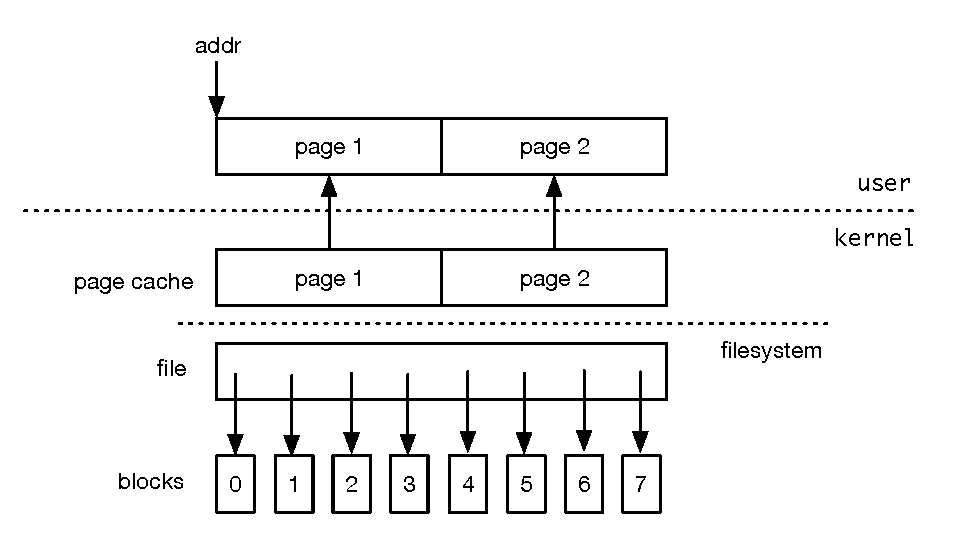
\includegraphics[scale=0.6]{figures/mmap-example.pdf}
	\centering
	\caption{Mapping an 8 KB file into memory}
	\label{fig:mmap-example}
\end{figure}

As we walk through the mapping, the kernel will call the filesystem to bring data into memory. This data is cached in the Linux page cache in the kernel. Here, two pages are allocated. Data is then copied from the kernel pages into the user pages starting at address \cf{addr}. If we run the program again, it is very likely that the pages in the Linux page cache will still be present so no more I/O will take place.

%------------------------------------------------------------------------------------------------------------------------------------------------------------------------

\subsection{The \cf{mmap(2)} / \cf{munmap()} System Calls}

The definition of \cf{mmap(2)} and \cf{munmap(2)} are as follows:

\begin{lstlisting}
void *mmap(void *addr, size_t length, int prot, int flags,
           int fd, off_t offset);
			  
int   munmap(void *addr, size_t length);
\end{lstlisting}

\noindent
The \cf{addr} argument is a hint as to where the region of the file will be mapped in memory. It must be correctly aligned according to the architecture on which the process is running. A page-aligned address should be used. The \cf{prot} argument specifies the memory protection of the mapping and can be one of the following:

\begin{itemize}
	\item \cf{PROT\_EXEC} -- pages may be executed.
	\item \cf{PROT\_READ} -- pages may be read.
	\item \cf{PROT\_WRITE} -- pages may be written.
	\item \cf{PROT\_NONE} -- pages may not be accessed.
\end{itemize}

\noindent
The \cf{flags} argument can be one of 20 different values. A few of the more widely used flags are:

\begin{itemize}
	\item \cf{MAP\_SHARED} -- the mapping can be shared with other processes .  Updates to the mapping are visible to other
              processes  mapping  the  same  region of the file, and changes made by any process are carried through to the 
              underlying  file.
	\item \cf{MAP\_PRIVATE} -- create a private copy-on-write mapping.  Any updates to the  mapping
              are  not  visible  to other processes mapping the same part of the file, and are not carried through to the underlying file.  
	\item \cf{MAP\_FIXED} -- don't interpret \cf{addr} as a hint and place  the  mapping  at  exactly the address specified 
		by \cf{addr}.
\end{itemize}

\noindent
The \cf{fd} argument specifies the file to be mapped and the \cf{offset} argument is an offset within the file. It should be a multiple of the system's page size.

The \cf{munmap(2)} system call can be called to delete the mapping for the specified address range (\cf{addr} and \cf{length}. Subsequent references to addresses within the range being unmapped will generate \cf{SIGSEGV}.  The  \cf{addr} argument must be a multiple of the page size (but the \cf{length} argument need not  be).   

%------------------------------------------------------------------------------------------------------------------------------------------------------------------------

\subsection{Other Mapped File Functions}

There are several other functions related to file mappings that are highlighted below:

\begin{itemize}
	\item \cf{msync(2)} -- flush changes made to the mapping back to the underlying file. An address and length are specified
		with flags indicating whether to perform writes synchronously, asynchronously and whether to invalidate any other  	
		mappings of the file so that subsequent access will bring in the new changes from disk.
	\item \cf{mlock(2)} / \cf{mlock2(2)} \cf{mlockall(2)} -- lock a number or all pages into memory to prevent them from
		being written to swap. A call to \cf{mlock2(2)} differs only if a flag of \cf{MLOCK\_ONFAULT} is specified in
		which case resident pages are locked and if pages within the mapping are current paged out, they will be 
		locked once they are faulted back into memory.
	\item \cf{mprotect(2)} -- when a call to \cf{mmap(2)} is made, the \cf{prot} argument specifies the access protections
		(for example \cf{PROT\_READ} or \cf{PROT\_READ}. This call allows those protections to be changed for an
		existing mapping. There are some additional access protections that are not part of the original \cf{mmap(2)}
		system call.
	\item \cf{mremap(2)} -- expands or shrinks an existing memory mapping and potentially moving the mapping at the same time
		depending on what flags are specified.
\end{itemize}
       
\noindent
Executables and corresponding libraries can be very large and it's unknown as to how much of the program binary will be used. The best method of reducing memory usage and I/O is to use \textit{demand paging}. The loader will establish a mapping to the executable as well as the various dynamic libraries that the program is linked with. When the process starts executing it will only bring in pages that are accessed. To further reduce memory, the mappings to program binaries and libraries are shared between processes. Program executables only need read access.

%%%%%%%%%%%%%%%%%%%%%%%%%%%%%%%%%%%%%%%%%%%%%%%%%%%%%%%%%%%%%%%

\section{Asynchronous I/O}

The \cf{read(2)} and \cf{write(2)} system calls are synchronous, that is, each operation will not return until the data is read/written or an error condition occurs. Depending on the type of I/O, the Linux kernel may have to call the filesystem which may have to go to disk to complete the operation. This is a time-consuming task compared to what an application could be doing if it solely operated on data in memory. While vectored reads/writes allow multiple I/Os to take place during a single call, likely improving performance, the application will still pause until the operation completes. Further optimizations can take place with threads which we will discuss in the next section. But prior to the widespread availability of \textit{pthreads} (process threads), asynchronous I/O, commonly called async I/O, was introduced whereby I/O operations could be started and the application would be notified asynchronously at a later time when the operation(s) completes. This allows the application to perform other tasks. One of the main drivers for async I/O, were the commercial databases such as Oracle. 

The \cf{aio(7)} manpage describes the different async I/O functions available. There is quite a lot to explain about these functions, but starting with the read/write interfaces:

\begin{lstlisting}
#include <aio.h>

int aio_read(struct aiocb *aiocbp);
int aio_write(struct aiocb *aiocbp);
int lio_listio(int mode, struct aiocb *restrict const 
               aiocb_list[restrict], int nitems, 
               struct sigevent *restrict sevp);
\end{lstlisting}

\noindent
The first two functions initiate single read/write operations while \cf{lio\_listio(3)} initiates the list of I/O operations described by the array \cf{aiocb\_list}. The \cf{aiocb} structure (aync I/O control block or AIO control block) contains the parameters used to specify the I/O operation or operations. It is defined in the \cf{aiocb.h} header file as follows:

\begin{lstlisting}
struct aiocb {
   int             aio_fildes;     /* File descriptor */
   off_t           aio_offset;     /* File offset */
   volatile void  *aio_buf;        /* Location of buffer */
   size_t          aio_nbytes;     /* Length of transfer */
   int             aio_reqprio;    /* Request priority */
   struct sigevent aio_sigevent;   /* Notification method */
   int             aio_lio_opcode; /* Operation to be performed; 
                                      lio_listio() only */                                     
}
\end{lstlisting}

\noindent
The first four fields will be recognizable as they are similar the arguments that would be passed to \cf{pread(2)} or \cf{pwrite(2)} so basically a call to \cf{lseek(2)} followed by a read or write. The \cf{aio\_reqprio} field specifies the relative priority of the I/O request. If the process priority is X and \cf{aio\_reqprio} is 6, the resulting priority of the I/O task is 10 - 6 = 4. \textbf{XXX--- need to come back to this}

\cf{aio\_lio\_opcode} is used by \cf{lio\_listio(3)} only and can be one of the following depending on what the operation is to perform:

\begin{lstlisting}
enum { LIO_READ, LIO_WRITE, LIO_NOP };
\end{lstlisting}

\noindent
The \cf{lio\_listio(3)} function can perform a mix of reads and writes with a single call. By setting  \cf{aio\_lio\_opcode} is set to \cf{LIO\_NOP} that specific AIO control block is ignored. 

The \cf{aio\_sigevent} specifies the mechanism through which the application is notified when the async I/O operation completes.

\begin{lstlisting}
struct sigevent {
    int             sigev_notify; /* Notification type */
    int             sigev_signo;  /* Signal number */
    union sigval    sigev_value;  /* Signal value */
    void          (*sigev_notify_function)(union sigval);
                                  /* Notification function */
    pthread_attr_t *sigev_notify_attributes;
                                  /* Notification attributes */
};
\end{lstlisting}

\noindent
I won't go into the details of each field of this structure but the example below will show how it is used. Refer to the \cf{sigevent(7)} manpage for more information.

To demonstrate how async I/O works in practice, we will givean example of how to issue multiple async I/Os to the same but using the \cf{lio-listio()} function. Figure \ref{fig:asyncio} shows a file contains 10 \cf{0}s followed by 10 \cf{1}s, 10 \cf{2}s and so on. Our goal is to read the \cf{1}s in an area of memory referenced by \cf{buf1}, overwrite the \cf{2}s with the contents of the memory referenced by \cf{buf2} and read the \cf{3}s in an area of memory referenced by \cf{buf3}.

\begin{figure}
	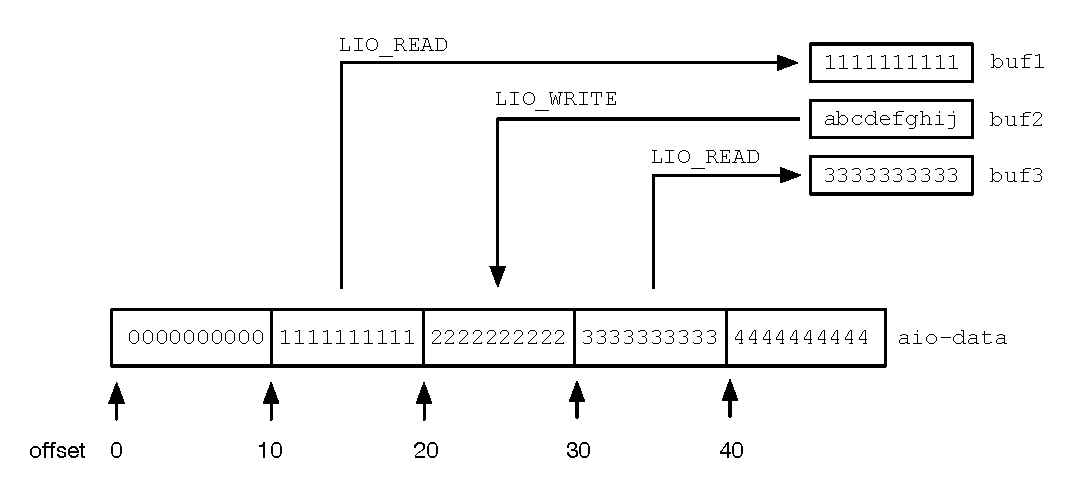
\includegraphics[scale=0.6]{figures/asyncio.pdf}
	\centering
	\caption{Reading and writing from/to a file using async I/O}
	\label{fig:asyncio}
\end{figure}

Most of the program involves setting up our three AIO control blocks which we do in lines 31-45 after opening our file \cf{aio-data}.

\begin{lstlisting}
 1 #include <fcntl.h>
 2 #include <aio.h>
 3 #include <signal.h>
 4 #include <stdio.h>
 5 #include <string.h>
 6 #include <unistd.h>
 7 #include <sys/uio.h>
 8 
 9 char *buf2 = "abcdefghij";
10 char buf1[32];
11 char buf3[32];
12 
13 void
14 aio_hdlr(int signo)
15 {
16     printf("buf1 = %.10s\n", buf1);
17     printf("buf3 = %.10s\n", buf3);
18 }
19 
20 int
21 main(int argc, char *argv[])
22 {
23     struct sigaction act;
24     struct sigevent  sevp;
25     struct aiocb     *list_aio[3];
26     struct aiocb     aio1, aio2, aio3;
27     int              err, fd;
28 
29     fd = open("aio-data", O_RDWR);
30 
31     aio1.aio_fildes  = fd;   aio1.aio_lio_opcode = LIO_READ;
32     aio1.aio_buf     = buf1; aio1.aio_offset     = 10;
33     aio1.aio_nbytes  = 10;   aio1.aio_reqprio    = 0;
34 
35     aio2.aio_fildes  = fd;   aio2.aio_lio_opcode = LIO_WRITE;
36     aio2.aio_buf     = buf2; aio2.aio_offset     = 20;
37     aio2.aio_nbytes  = 10;   aio2.aio_reqprio    = 0;
38 
39     aio3.aio_fildes  = fd;   aio3.aio_lio_opcode = LIO_READ;
40     aio3.aio_buf     = buf3; aio3.aio_offset     = 30;
41     aio3.aio_nbytes  = 10;   aio3.aio_reqprio    = 0;
42 
43     list_aio[0] = &aio1;
44     list_aio[1] = &aio2;
45     list_aio[2] = &aio3;
46 
47     memset(&act, 0, sizeof(act));
48     act.sa_handler = aio_hdlr;
49     sigaction(SIGUSR1, &act, NULL);
50     act.sa_handler = SIG_IGN;
51     sigaction(SIGHUP, &act, NULL);
52 
53     memset(&sevp, 0, sizeof(sevp));
54     sevp.sigev_signo = SIGUSR1;
55     sevp.sigev_notify = SIGEV_SIGNAL;
56     sevp.sigev_value.sival_ptr = (void *)list_aio;
57 
58     err = lio_listio(LIO_NOWAIT, list_aio, 3, &sevp);
59     pause();
60 }
\end{lstlisting}

\noindent
\textbf{XXX---need to either explain the issue with SIGHUP or fix it!!! - also, perhaps we can have the signal handler analyze the aiocbs (re sigevent) otherwise all that stuff on 53-56 is kind of wasted}

Additional info about the program is as follows:

\begin{itemize}
	\item Lines 47 - 51 -- When the async I/O operations complete the program will be notified by a signal. 
		I'm choosing \cf{SIGUSR1} as the signal to use and my signal handler is the function \cf{aio\_hdlr}.
		Lines 47 - 49 provide the set up needed. \textbf{XXX---SIGHUP dunno}
	\item Lines 53 - 56 -- \cf{lio\_listio(3)} requires a pointer to a \cf{sigevent} structure which tells it which
		signal to post and a pointer to a structure which will be passed to the signal handler. This allows
		the program to check for the status of individual I/O operations. For more details about how async I/O
		uses signal handler, refer to the \cf{sigevent(7)} manpage.
	\item Line 58 -- Call \cf{lio\_listio(3)} to initiate the I/O operations.
	\item Line 59 -- Pause the program to wait for signal handling. Once the signal handler runs, 
		\cf{pause(2)} returns and the program will exit.
\end{itemize}

\noindent
Before running the program, we display the contents of the \cf{aio-data} file, then run the program and then display the file contents again. As you can see, \cf{buf1} and \cf{buf2} contain the data expected and \cf{aio-data} is overwritten at offset 20 with the string \cf{abcdefghij} referenced by \cf{buf2}.

\begin{lstlisting}
$ [*\bfseries cat aio-data*]
00000000001111111111222222222233333333334444444444
$ [*\bfseries ./aio*]
buf1 = 1111111111
buf3 = 3333333333
$ [*\bfseries cat aio-data*]
00000000001111111111abcdefghij33333333334444444444
\end{lstlisting}

%----------------------------------------------------------------------------------------------------------------------------------------------------------------

\subsection{Additional Async I/O Functions}

There are several other functions available that are needed to build enterprise applications and worth exploring. They are highlighted below. Also, view the \cf{aio(7)} manpage for additional information.

\begin{itemize}
       \item \cf{aio\_fsync(3)} --- Queue a \textit{sync} request for the I/O operations on the file descriptor specified
       		in the AIO control block. This is somewhat equivalent to calling of \cf{fsync(2)} and \cf{fdatasync(2)}. 
		If the \cf{op} argument is \cf{O\_SYNC}, then all currently queued I/O operations shall 
		be completed as if by making a call to \cf{fsync(2)}, and if \cf{op} is \cf{O\_DSYNC}, this call is the 
		asynchronous analog of \cf{fdatasync(2)}. This function doesn't wait for I/Os to completion.

       \item \cf{aio\_error(3)} --- Obtain  error status of a queued I/O request.

       \item \cf{aio\_return(3)} --- Obtain the return status of a completed I/O request.

       \item \cf{aio\_suspend(3)} --- Suspend the caller until one or more of a specified set of I/O requests completes.

       \item \cf{aio\_cancel(3)} --- Attempt to cancel outstanding I/O requests on a specified file descriptor.
\end{itemize}

%%%%%%%%%%%%%%%%%%%%%%%%%%%%%%%%%%%%%%%%%%%%%%%%%%%%%%%%%%%%%

\subsection{Performance Gains with Async I/O}

Disks have come a long way since the POSIX async I/O standard was being developed back in the early 1990s. But even with  faster disks, disk subsystems and SSDs, it's still slow to \textit{go to disk} compared with reading from an in-core cache, whether the Linux page cache or a database cache. Also recall that at the time of the async I/O standard being developed, CPU cores were non-existent and the multi-threading standard known as pthreads was still being developed. When I was at ICL (International Computers Limited), we were implementing async I/O on SVR4 UNIX implementation on top of the Chorus microkernel to support Oracle. I recall the performance gains made by the database to be huge although it was a long time ago so I don't recall the details.

\begin{quote}
You don't have to worry about threading or race conditions or losing error state (as much). AFIO does all that for you.
On platforms which provide native asynchronous file i/o support and/or native scatter/gather file i/o support, AFIO will use that instead of issuing multiple filing system operations using a thread pool to achieve concurrency. This can very significantly reduce the number of threads needed to keep your storage device fully occupied — remember that queue depth i.e. that metric you see all over storage device benchmarks is the number of operations in flight at once, which implies the number of threads needed. Most storage devices are IOPS limited due to SATA or SAS connection latencies without introducing queue depth — in particular, modern SSDs cannot achieve tens of thousands of IOPS range without substantial queue depths, which without using a native asynchronous file i/o API means lots of threads.
It's very, very easy to have AFIO turn off file system caching, readahead or buffering on a case by case basis which makes writing scalable random synchronous file i/o applications much easier.
\end{quote}

\textbf{XXX---need to come back and enhance once the FS performance chapter is finished}

Oracle but any info? Not easy to find.

Lighty - http://blog.lighttpd.net/articles/2006/11/12/lighty-1-5-0-and-linux-aio/ 

wikipedia - %https://en.wikipedia.org/wiki/Asynchronous_I/O 

just search for "application+performance+gains+examples" - there are lots of examples

%----------------------------------------------------------------------------------------------------------------------------------------------------------------

\subsection{procfs Async I/O Information}

There are two files in the proc file system that can be tuned for asynchronous I/O. Both can be found under \cf{/proc/sys/fs}:

\begin{itemize}
	\item \cf{aio-nr} --- the current number of system-wide asynchronous I/O requests. If there are no
		async I/O requests active, this number will be 0.
	\item \cf{aio-max-nr} --- the maximum number of allowable concurrent requests. This is generally 64 KB.
\end{itemize}

%%%%%%%%%%%%%%%%%%%%%%%%%%%%%%%%%%%%%%%%%%%%%%%%%%%%%%%%%%%%%

\section{Truncating Files}\label{prog-truncate}

When describing the \cf{open(2)} system call in section \ref{prog-open-flags}, the \cf{O\_TRUNC} flag can be passed to ensure that the file is truncated to length of zero if the file already exists. If a file needs to be truncated either without opening it or after the file is opened, the following system calls can be used:

\begin{lstlisting}
#include <unistd.h>

int truncate(const char *path, off_t length);
int ftruncate(int fd, off_t length);
\end{lstlisting}

\noindent
The difference between using \cf{O\_TRUNC} during a call to \cf{open(2)} and the above interfaces is that the file will be truncated to exactly \cf{length} bytes.

A file can be truncated down in size or it can be truncated up. I always found that amusing when I very first saw this descriptioin many years ago. How do you allocate space to a file? "Truncate the file up"!

If the size of the file is larger than the size specified by \cf{length}, the extra data will be lost following the truncation.  If the file is shorter, it will be is extended. The extended part will read as null bytes ('\cf{\textbackslash0'}).

%%%%%%%%%%%%%%%%%%%%%%%%%%%%%%%%%%%%%%%%%%%%%%%%%%%%%%%%%%%%%

\section{Multi-threaded Applications}

There have been several books written about multi-threaded applications and for the most part, multi-threading is beyond the scope of this chapter. The following web page gives a very good introduction into multi-threading and introduces not just multi-threading concepts but also pthreads, POSIX threads, the default method of multi-threading on Linux.

\begin{table}[h]
\begin{tabular}{lcl}
\parbox[r]{0.5in}{
\includegraphics[scale=0.15]{figures/url.png}} & \parbox[l]{0.55in}{URL \arabic{urls}} & \parbox[l]{3in}{\cf{https://tinyurl.com/5ssbe8db}}
\end{tabular}
\end{table}
\stepcounter{urls}
% https://randu.org/tutorials/threads/

\noindent
The \cf{pthreads(7)} manpage is the place to start to learn about the programming interfaces available that underpin pthreads. Over the last twenty years, Linux has seen two different implementations for pthreads:

\begin{itemize}
	\item LinuxThreads -- the original Pthreads implementation which, since glibc  2.4, is no longer supported.
	\item NPTL (Native POSIX Threads Library) -- the modern pthreads implementation.  By comparison with
              LinuxThreads, NPTL provides closer conformance to  the  requirements  of  the POSIX.1 specification than 
              LinuxThreads. It also has better performance when creating large numbers of  threads.  NPTL  has been 
              available  since glibc 2.3.2, and requires features that are present since the Linux 2.6 kernel.
\end{itemize}

\noindent
Start with \cf{pthreads(7)} and go from there. Most articles on line will reference the newer implementation. The \cf{getconf(1)} command can be used to determine which implementation is available:

\begin{lstlisting}
$ [*\bfseries getconf GNU\_LIBPTHREAD\_VERSION*]
NPTL 2.36
\end{lstlisting}

\noindent
When developing applications that access files / filesystems, there aren't many things to bear in mind when writing multi-threaded applications:

\begin{itemize}
	\item All open files are shared between all process threads. If a thread (other than \cf{main()}) opens a file, it should 
		be closed before the thread terminates.
	\item Linux file locking has issues when deploying multi-threaded applications. Please refer to section \ref{prog-locking}
		and make sure you use the newer \textit{Open File Description Locks}. 
	\item It should go without saying that any change that any thread makes, including calls resulting in a state change
		in the kernel, are visible to all other threads. Since file descriptors are shared, offsets within each file are
		also shared.
\end{itemize}

%%%%%%%%%%%%%%%%%%%%%%%%%%%%%%%%%%%%%%%%%%%%%%%%%%%%%%%%%%%%%

\section{Directory Creation}\label{prog-mkdir}

Directory creation is handled by the \cf{mkdir(2)} and \cf{mkdirat(2)} system calls:

\begin{lstlisting}
#include <sys/stat.h>

int mkdir(const char *pathname, mode_t mode);

#include <fcntl.h>           /* Definition of AT_* constants */ 
#include <sys/stat.h>

int mkdirat(int dirfd, const char *pathname, mode_t mode);
\end{lstlisting}

\noindent
For \cf{mkdir(2)}, the pathname can be absolute or relative. The \cf{mode} argument specifies the mode for the newly created directory. It is modified by the process's umask using the formula (\cf{mode \& \~{}umask \& 0777}).

How the \cf{mkdirat(2)} system call operates depends on \cf{pathname}. Either:

\begin{itemize}
	\item If \cf{pathname} is relative, it is interpreted relative to the directory referred to  by  the  file  descriptor  \cf{dirfd}
		as opposed to being relative to the current working directory of the calling process (as is done by \cf{mkdir(2)} 
		for a relative pathname).
	\item If \cf{pathname} is relative and \cf{dirfd} is set to \cf{AT\_FDCWD},  \cf{pathname} is interpreted relative to 
		the current working directory of the calling process (as for \cf{mkdir(2)}).
	\item If \cf{pathname} is absolute, \cf{dirfd} is ignored.
\end{itemize}

\noindent
Removing a directory is very straightforward:

\begin{lstlisting}
#include <unistd.h>

int rmdir(const char *pathname);
\end{lstlisting}

\noindent
The directory must be empty before this operation can succeed.

%%%%%%%%%%%%%%%%%%%%%%%%%%%%%%%%%%%%%%%%%%%%%%%%%%%%%%%%%%%%%

\section{Hard Links and Symbolic Links}\label{prog-links}

Creating a hard link with the \cf{link(2)} or \cf{linkat(2)} system calls involves creation of a new directory entry that references the file to which it is linked to. Following a successful call, the file referenced by \cf{newpath} can be used in exactly the same manner as the file \cf{oldpath}, to which it is linked.

\begin{lstlisting}
#include <unistd.h>

int link(const char *oldpath, const char *newpath);

#include <fcntl.h>           /* Definition of AT_* constants */ 
#include <unistd.h>

int linkat(int olddirfd, const char *oldpath,
           int newdirfd, const char *newpath, int flags);
\end{lstlisting}

\noindent
Below is a simple example showing the effects of calling \cf{link(2)}. All the program does is create a hard link called "\cf{latin-text}" to the existing file "\cf{lorem-ipsum}".

\begin{lstlisting}
#include <unistd.h>

int
main()
{
    link("lorem-ipsum", "latin-text");
}
\end{lstlisting}

\noindent
Before the program is run, the attributes of "\cf{lorem-ipsum}" are displayed. The link count for this file is "1". The program is then run and the link count goes to "2". When the attributes of "\cf{latin-text}", you can see they mirror the attributes of "\cf{lorem-ipsum}".

\begin{lstlisting}
$ [*\bfseries ls -li lorem-ipsum *]
409993 -rw-r--r-- [*\bfseries 1*] spate spate 2972 Apr  4 16:43 lorem-ipsum
$ [*\bfseries ./link*]
$ [*\bfseries ls -li lorem-ipsum*] 
409993 -rw-r--r-- [*\bfseries 2*] spate spate 2972 Apr  4 16:43 lorem-ipsum
$ [*\bfseries ls -li latin-text  *]
409993 -rw-r--r-- [*\bfseries 2*] spate spate 2972 Apr  4 16:43 latin-text
$ [*\bfseries diff lorem-ipsum latin-text  *]
\end{lstlisting}

\noindent
The \cf{linkat(2)} system call differs from \cf{link(2)} primarily in how the two files are referenced. See the previous section on how \cf{mkdirat(2)} operates. The main difference here is that there is an additional \cf{flags} argument which can be a bitwise OR of the following:

\begin{itemize}
	\item \cf{AT\_EMPTY\_PATH} -- If \cf{oldpath} is an empty string then the link will be created to reference the file
		\cf{olddirfd}.
	\item \cf{AT\_SYMLINK\_FOLLOW} -- By default, \cf{oldpath} will not be dereferenced if it is a symbolic  link, the same
		being is true with \cf{link(2)}).  If \cf{AT\_SYMLINK\_FOLLOW} is specified in \cf{flags} and \cf{oldpath} is a symbolic 
		link, it will be dereferenced.
\end{itemize}

\noindent
The \cf{unlink(2)} and  \cf{unlinkat(2)} system calls can be used to remove a link to a file:

\begin{lstlisting}
#include <unistd.h>

int unlink(const char *pathname);

#include <fcntl.h>           /* Definition of AT_* constants */
#include <unistd.h>

int unlinkat(int dirfd, const char *pathname, int flags);
\end{lstlisting}

\noindent
 If \cf{pathname} is the last link to a file and no processes have the file open, the file will deleted and any space it is using will be reclaimed and made available for other use. If \cf{pathname} references a symbolic link, only the link is removed.
 
 The \cf{unlinkat(2)} system call operates the same way as both \cf{unlink(2)} and \cf{rmdir(2)}. If the \cf{flag} argument is \cf{AT\_REMOVEDIR}, the equivalent of \cf{rmdir(2)} will be performed.
 
%%%%%%%%%%%%%%%%%%%%%%%%%%%%%%%%%%%%%%%%%%%%%%%%%%%%%%%%%%%%
 
 \subsection{Symbolic Links}
 
The \cf{symlink(2)} system call creates a symbolic link called \cf{linkpath}. It will contain the string \cf{target}. The existence of the target file is not checked during this operation.
 
\begin{lstlisting}
#include <unistd.h>

int symlink(const char *target, const char *linkpath);

#include <fcntl.h>           /* Definition of AT_* constants */ 
#include <unistd.h>

int symlinkat(const char *target, int newdirfd, 
              const char *linkpath);
\end{lstlisting}

\noindent
The \cf{symlinkat(2)} system call operates in the same way as \cf{symlink(2)} with the following two exceptions:

\begin{itemize}
	\item If \cf{linkpath} is relative, it will be interpreted relative to the directory referred to by the file descriptor \cf{newdirfd}.
	\item If  \cf{linkpath} is relative and \cf{newdirfd} is the value \cf{AT\_FDCWD}, \cf{linkpath} is interpreted relative to the 
		current working directory of the calling process (like symlink()).
\end{itemize}

%%%%%%%%%%%%%%%%%%%%%%%%%%%%%%%%%%%%%%%%%%%%%%%%%%%%%%%%%%%%%

\section{Extended Attributes}

A file contains both the regular stream of data as written by applications in addition to meta-data created and maintained by the filesystem. User-visible meta-data can be obtained by running one of the \cf{stat(2)} system calls. Application developers pushed the operating system and small number of filesystem vendors for years to have them store user-defined attributes. As a specific example, back in the early to mid 1990s, I used to be a member of DMIG (the Data Management Interfaces Group) who were building storage management APIs to support Hierarchical Storage Management (HSM) applications. To save space on disk storage, HSM applications would punch holes in files accessed less frequently and store that data on tape to be read back at a later time when the file was accessed. This was a complex process and required per-file meta-data about the data being migrated to tertiary storage. At this time few vendors support such \textit{extended attributes}. But this was the beginning of what would become a POSIX standard. 

Today, the following filesystems in Linux support extended attributes---ext2, ext3, ext4, JFS, XFS, btrfs, OCFS2 and squashfs. Extended attributes have a name and associated data. Attribute names can be up to 255 characters and the size of the associated data is variable depending on the filesystem.

Linux provides four namespaces for extended file attributes:

\begin{enumerate}
	\item user
	\item trusted
	\item security
	\item system
\end{enumerate}

\noindent
The name of the attribute must start with one of the four names shown above followed a "." and then followed an application supplied name. An example could be \cf{user.comment}. The \cf{xattr(2)} manpage contains details about the different extended attribute system calls and commands. The \cf{setfattr(1)} and \cf{getfattr(1)} commands can be used to set and get extended attribute. The systems calls are \cf{setxattr(2)}, \cf{getxattr(2)}, \cf{removexattr(2)} and \cf{listxattr(2)} (which is used by "\cf{getfattr -d}").

\subsection{Installing and Using Extended Attributes}

On Ubuntu you need to install the \cf{attr} package as follows:

\begin{lstlisting}
$ [*\bfseries sudo apt install attr*]
\end{lstlisting}

\noindent
in order to start using extended attributes. In the example below, \cf{ls} is run against the file "\cf{lorem-ipsum}", an attribute is added and then \cf{ls} is run again. You'll see that the file looks exactly the same.

\begin{lstlisting}
$ [*\bfseries ls -l lorem-ipsum*]
-rw-r--r-- 1 spate spate 2972 Dec  4 15:43 lorem-ipsum
$ [*\bfseries setfattr -n user.comment -v "File contains Latin" lorem-ipsum*]
$ [*\bfseries ls -l lorem-ipsum*]
-rw-r--r-- 1 spate spate 2972 Dec  4 15:43 lorem-ipsum
\end{lstlisting}

\noindent
Extended attributes stored in a file can bee read the contents as follows:

\begin{lstlisting}
$ [*\bfseries getfattr -d lorem-ipsum*]
# file: lorem-ipsum
user.comment="File contains Latin"
\end{lstlisting}

\noindent
Despite demand for extended attributes over the years, their adoption has been somewhat limited. On Linux, The Wikipedia page on extended attributes mentions that they are used by Beagle, OpenStack Swift, Dropbox, KDE's semantic metadata framework (Baloo), Chromium, Wget and cURL. Desktop file manager usage has always been one of the most quoted examples but generally speaking, unless all underlying filesystems support extended attributes, the presentation to the user becomes more difficult to implementers since they can use extended attributes where available but then must use some other mechanism for storing attributes if the underlying filesystem does not support them. This results in a less than stellar presentation or an awkward implementation.

%%%%%%%%%%%%%%%%%%%%%%%%%%%%%%%%%%%%%%%%%%%%%%%%%%%%%%%%%%%%%

\section{Inode Flags}

Some of the Linux filesystems support the notion of \textit{inode flags} which are described in the \cf{ioctl\_iflags(2)} manpage. Inode flags are attributes used to modify the semantics of files and directories. These flags can be retrieved and modified using the following two \cf{ioctl(2)} operations:

\begin{lstlisting}
int attr, fd;

fd = open("filename", ...);
ioctl(fd, FS_IOC_GETFLAGS, &attr);  // get current flags
attr |= FS_NOATIME_FL;              // set the flags you want
ioctl(fd, FS_IOC_SETFLAGS, &attr);  // update the file's flags
\end{lstlisting}

\noindent
The first call retrieves the current flags and puts then in \cf{attr}. The bitmask is then modified and a second call is made to set the new flags. There are 14 flags in total and changes apply even if the caller has superuser privileges. Here are a few of the available flags:

\begin{itemize}
	\item \cf{FS\_APPEND\_FL} --  prevent the file from being opened only with  \cf{O\_APPEND}.
	\item \cf{FS\_IMMUTABLE\_FL} -- the file will be set to be immutable; no subsequent changes can be made to the 
		file contents or metadata.
	\item \cf{FS\_SYNC\_FL} -- make all future writes synchronous.
	\item \cf{FS\_NOATIME\_FL} -- the file's access time (atime) will not be update on access. This can have significant
		performance benefits.
\end{itemize}

\noindent
Inode flags are Linux specific, not part of any standard and not implemented by all of the Linux filesystems.

%%%%%%%%%%%%%%%%%%%%%%%%%%%%%%%%%%%%%%%%%%%%%%%%%%%%%%%%%%%%%

\section{Reading Directory Entries}\label{prog-readdir}

As you will see later in the book, parsing pathnames and handling directory entries is a complex task for both the kernel and filesystems to handle. In fact, supporting a very large number of files inside a single directory is a particularly complex task for filesystem developers.

Reading directory entries is performed by the \cf{readdir(3)} library function which is passed a \cf{DIR} structure, called a \textit{directory stream}, obtained from calling \cf{opendir(3)}. Both functions are defined as follows:

\begin{lstlisting}
#include <sys/types.h>
#include <dirent.h>

DIR *opendir(const char *name);
DIR *fdopendir(int fd);
int closedir(DIR *dirp);

struct dirent *readdir(DIR *dirp);
\end{lstlisting}

\noindent
For \cf{opendir(3)}, the \cf{name} argument should reference a directory either as a relative or absolute pathname. On return, the directory stream will be positioned ready to read the first entry in the directory. The \cf{fopendir(3)} library function also returns a directory stream but using a specified file descriptor. Note that the file descriptor should not be used for any other operation. The \cf{closedir(3)} function closes the directory stream as well as the underlying file descriptor.

Given a directory stream, an application can make calls to \cf{readdir(3)} with each call returning the next directory entry with each entry defined by the \cf{dirent} structure. I've only included three of the fields of this structure. Only the first two fields are required by POSIX. In the following section, I'll show an example of a simple version of the \cf{ls(1)} command which uses the first two fields but then uses the \cf{lstat(2)} system call to get the file type.

\begin{lstlisting}
struct dirent {
    ino_t          d_ino;       /* Inode number */
    char           d_name[256]; /* Null-terminated filename */
    unsigned char  d_type;      /* Type of file */
};
\end{lstlisting}

\noindent
Once all directory entries have been returned, the return value will be \cf{NULL}. You should not make any assumption about the order in which directory entries are returned. This will likely different from one filesystem to the next. 

%------------------------------------------------------------------------------------------------------------------------------------------------------------------------

\subsection{A Simple Implementation of the \cf{ls(1)} Command}\label{ls-command}

To give an example of how \cf{readdir(3)} can be used, here is a simple version of the \cf{ls(1)} command which does the equivalent of \cf{ls -al} on the current directory. The source code to our minimal \cf{ls} command is shown below. For the \cf{print\_*} functions, the source code is available at the book's github site. There is a fair amount of processing of the \cf{stat} structure, mapping between UID/GID and actual string representations and manipulation of the modification time to get it into the right format. 

\begin{lstlisting}
 1 int
 2 main() {
 3     struct dirent *dir;
 4     DIR           *mydir;
 5     struct stat   st;
 6  
 7     mydir = opendir(".");
 8     while (1) {
 9         dir = readdir(mydir);
10         if (dir == NULL) {
11             break;
12         }
13         lstat(dir->d_name, &st);
14         print_file_type(&st);
15         print_perms(&st);
16         printf(" %d ", st.st_nlink);
17         print_owner_group(&st);
18         printf("%5ld ", st.st_size);
19         print_mtime(&st);
20         printf("%s\n", dir->d_name);
21     }
22 }
\end{lstlisting}

\noindent
The program is quite simple, looping through the directory making calls to \cf{readdir(3)} (line 9) to read each directory entry. Once the last entry has been read, \cf{NULL} will be returned. Then for each directory entry read, we print out the various fields to match the output returned by running \cf{ls -al}.

As mentioned above, the \cf{d\_type} field of the \cf{dirent} structure is not POSIX compliant but could be used to avoid a call to \cf{lstat(2)}. In our example, we want more information about the file so this call is necessary. Furthermore, we need to call \cf{lstat(2)} in place or \cf{stat(2)} since, if this was a symbolic link, we would information about the symbolic link and not the file to which it points to.

The \cf{print\_file\_type()} function simply checks the \cf{S\_IFMT} field of the \cf{stat} structure. Here is a fragment of the source code:

\begin{lstlisting}
print_file_type(struct stat *st)
{
    char c;

    switch (st->st_mode & S_IFMT) {
        case S_IFBLK:
            c = 'b';
            break;
        case S_IFCHR:
            c = 'c';
            break;
        ...
        default:
            c = '?';
            break;
    }
    printf("%c", c);
}
\end{lstlisting}

\noindent
Below is output from the program running showing contents of a directory with several different file types followed by running the real \cf{ls -l}:

\begin{lstlisting}
$ [*\bfseries ./myls*]
brw-r--r-- 1 root  root      0 Dec 19 17:41 mydev
drwxrwxr-x 2 spate spate  4096 Dec 19 17:39 mydir
drwxrwxr-x 3 spate spate  4096 Dec 19 17:41 .
-rw-r--r-- 1 spate spate   325 Dec 19 17:39 sparse.c
prw-rw-r-- 1 spate spate     0 Dec 19 17:40 mypipe
drwxrwxr-x 4 spate spate  4096 Dec 19 19:41 ..
-rwxrwxr-x 1 spate spate 70504 Dec 19 17:39 fds
$ [*\bfseries ls -al*]
total 32
drwxrwxr-x 3 spate spate  4096 Dec 19 17:41 .
drwxrwxr-x 4 spate spate  4096 Dec 19 19:41 ..
-rwxrwxr-x 1 spate spate 70504 Dec 19 17:39 fds
brw-r--r-- 1 root  root   4, 5 Dec 19 17:41 mydev
drwxrwxr-x 2 spate spate  4096 Dec 19 17:39 mydir
prw-rw-r-- 1 spate spate     0 Dec 19 17:40 mypipe
-rw-r--r-- 1 spate spate   325 Dec 19 17:39 sparse.c
\end{lstlisting}

\noindent
The \cf{ls(1)} program does a lot of formatting. When you run \cf{ls -l}, the "." and ".." entries are displayed first. The spacing around the owner, group and file size are nicely done. This implies that \cf{ls} must make at least one pass through the list of directory entries before it starts printing anything. However, all entries are read using \cf{readdir(3)} and then a call is made to \cf{sort\_files()} to sort / format them. You can find the source code to the \cf{ls(1)} command here:

\begin{lstlisting}
https://github.com/wertarbyte/coreutils/blob/master/src/ls.c
\end{lstlisting}

\noindent
This simple version of \cf{ls} doesn't display the device file major/minor and won't nicely format directory entries if owner, group and size of more characters than those shown here.

%------------------------------------------------------------------------------------------------------------------------------------------------------------------------

\subsection{Other Directory Functions}

One of the most useful functions, and one which could simply our version of \cf{ls(1)} by getting an alphabetically sorted list of directory entries, is the \cf{scandir(3)}:

\begin{lstlisting}
#include <dirent.h>

int scandir(const char *restrict dirp,
           struct dirent ***restrict namelist,
           int (*filter)(const struct dirent *), 
           int (*compar)(const struct dirent **, 
                         const struct dirent **));
\end{lstlisting}

\noindent
The directory specified by \cf{dirp} is scanned and entries are sorted according to the function specified by \cf{comprar} which can be \cf{alphasort} which sorts directory entries using \cf{strcoll(3)}, or \cf{versionsort} which sorts using \cf{strverscmp(3)} on the strings \cf{(*a)->d\_name} and \cf{(*b)->d\_name}. As entries are being read, space is allocated by calling \cf{malloc(3)}. 

The \cf{filter} argument can be used to select specific entries. An an example, if our \cf{myls} program was given wildcards as an argument, the \cf{filter} function provided could be used to match specific files. If \cf{filter} is set to \cf{NULL} all directory entries will be returned. 

Here is a skeleton version of a program that we could have used for the \cf{myls} command above. Note that as we display each directory entry, we free the space that was allocated by \cf{scandir(3)}.

\begin{lstlisting}
#include <dirent.h>
#include <stdio.h>
#include <stdlib.h>

int
main(void)
{
   struct dirent **namelist;
   int nentries, i;

   nentries = scandir(".", &namelist, NULL, alphasort);
   for (i=0 ; i<nentries ; i++) {
       printf("%s\n", namelist[i]->d_name);
       free(namelist[i]);
   }
   free(namelist);

}
\end{lstlisting}

\noindent
Since we've passed \cf{alphasort} as an argument, we get all entries sorted nicely:

\begin{lstlisting}
$ [*\bfseries ./scandir*]
.
..
fds
mydev
mydir
mypipe
sparse.c
\end{lstlisting}

\noindent
There are other functions that allow you to browse directory trees which you can peruse at your own pleasure:

\begin{itemize}
	\item \cf{ftw(3)} --- Walk through a directory tree and calls the specified function for each entry in the tree.
	\item \cf{fts(3)} --- More functions for walking a directory tree.
	\item \cf{telldir(3)} --- Return current location in directory stream.
	\item \cf{seekdir(3)} --- Set the location in the directory  stream  from which  the next call to \cf{readdir(2)} 
		will start. A value returned by \cf{telldir(3)} should be used.
	\item \cf{rewinddir(3)} --- Reset the position of the directory stream to the beginning of the directory.
\end{itemize}

%------------------------------------------------------------------------------------------------------------------------------------------------------------------------

\subsection{Directory Entries at the System Call Level}

The library functions described in the sections above all build on top of a simple system call interface defined as follows in the \cf{getdents(2)} manpage:

\begin{lstlisting}
#include <sys/syscall.h>   /* Defn of SYS_* constants */
#include <unistd.h>

long syscall(SYS_getdents, unsigned int fd, 
             struct linux_dirent *dirp, unsigned int count);

#define _GNU_SOURCE.   /* See feature_test_macros(7) */
#include <dirent.h>

ssize_t getdents64(int fd, void *dirp, size_t count);
\end{lstlisting}

\noindent
As the manpage says:

\begin{quote}
\textit{These are not the interfaces you are interested in.  Look at readdir(3)
for the POSIX-conforming C library interface.  This page documents  the
bare kernel system call interfaces.}
\end{quote}

\noindent
If you browse the glibc source code, you'll see that it uses \cf{getdents64()} which returns one or more directory entries in the buffer pointed to by \cf{dirp}. The size of the buffer is referenced by \cf{count}. The number of entries read is returned and each entry returned is defined by the \cf{linux\_dirent} structure:

\begin{lstlisting}
struct linux_dirent64 {
    ino64_t        d_ino;    /* 64-bit inode number */
    off64_t        d_off;    /* 64-bit offset to next struct */
    unsigned short d_reclen; /* Size of this dirent */
    unsigned char  d_type;   /* File type */
    char           d_name[]; /* Filename (null-terminated) */
};
\end{lstlisting}

\noindent
Although it looks similar to \cf{readdir(3)} it requires a lot more work on behalf of the caller and thus the very large warning in the manpage. Applications should use the functions described earlier but it's important to highlight the system call since we will be describing its implementation later in the book in section \ref{vfs_readdir}.

%%%%%%%%%%%%%%%%%%%%%%%%%%%%%%%%%%%%%%%%%%%%%%%%%%%%%%%%%%%%%%%

\section{File Notification}\label{fanotify}

File notification is a mechanism where applications can be notified of events that occur within the filesystem in response to actions such a file creation, reads, writes and deletions.

There are several applications that can make use of filesystem notification events. Examples that come to mind are desktop file managers which can update their display of a directory as changes are made to the directory, malware scanners such as ClamAV and hierarchical storage management which is discussed elsewhere in the book. Another important example is backup. When determining what files to backup, scanning a filesystem looking for changes can be a time-consuming task. If the backup application already had a list of changed files, that scan could be avoided.

The three different file notification mechanisms that exist in Linux are as follows:

\begin{itemize}
	\item \textbf{dnotify} -- appearing in Linux in 2001, the first mechanism lacked the knowledge about how such frameworks
		should be used and relied on extensions to \cf{fcntl(2)}, for example "\cf{fcntl(fd, F\_NOTIFY, mask)}". Only
		directories could be monitored and not regular files. Delivery of a signal indicated notification of an event but the
		application needs to scan the directory to see what actually changed. There were additional shortcomings. 
	\item \textbf{inotify} -- first appearing in Linux 2.6.13 in 2005, the inotify framework intended to resolve the issues with
		dnotify. The three system calls, namely \cf{inotify\_init(2)}, \cf{inotify\_add\_watch(2)}, and \cf{inotify\_rm\_watch(2)}
		were introduced. An initialization call to \cf{inotify\_init(2)} returns a file descriptor which is used by the other
		inotify system calls. Files and directories can be added to the list of file objects to be monitored and the list and
		events could be added or removed. The \cf{inotify(7)} manpage lists all of the possible events. There are several
		advantages over dnotify. In additional to supporting regular files, the interface was simpler, there are more events
		and there is better information about each event received. For more details of inotify I recommend reading the
		lwn.net articles (search for "linux filesystem notification part".
	\item \textbf{fnotify} -- first appeared in Linux 2.6.37 in 2011 and will be described in this section. It has a superset
		of the inotify functionality. 
\end{itemize}

\noindent
With fanotify, it's possible to monitor a mounted filesystem as a whole unlike inotify. Despite being introduced in 2011, fanotify has seen several improvements over the years with major enhancements appearing in 2019 such as support for create, move, and delete events. These events were part of a \textit{directory events} addition at the time. 

Before describing how to use fanotify, there is an example  program at the following location that will be demonstrated here:

\begin{table}[h]
\begin{tabular}{lcl}
\parbox[r]{0.5in}{
\includegraphics[scale=0.15]{figures/url.png}} & \parbox[l]{0.55in}{URL \arabic{urls}} & \parbox[l]{3in}{\cf{https://tinyurl.com/2p9dmz2n}}
\end{tabular}
\end{table}
\stepcounter{urls}
% https://gist.github.com/jaypeche/497ac0c3ce36cdb7f5b9

\noindent
Note that you will likely need to replace the line that includes "\cf{linux/fanotify.h}" with the following:

\begin{lstlisting}
#include <sys/fanotify.h>
\end{lstlisting}

\noindent
To run the program, specify a directory (this example uses "\cf{mydir}") and events will be displayed as operations are performed on files within the specified directory:

\begin{lstlisting}
$ [*\bfseries sudo ./fanotify-example mydir*]
Started monitoring directory 'mydir'...
Received event in path '/home/spate/mydir/foo' pid=2813 (...): 
	FAN_OPEN
	FAN_CLOSE_WRITE
Received event in path '/home/spate/mydir/foo' pid=1045 (-bash): 
	FAN_OPEN
Received event in path '/home/spate/mydir/foo' pid=1045 (-bash): 
	FAN_MODIFY
Received event in path '/home/spate/mydir/foo' pid=1045 (-bash): 
	FAN_CLOSE_WRITE
\end{lstlisting}

\noindent
The messages displayed are in response to the following operations:

\begin{lstlisting}
$ [*\bfseries touch mydir/foo*]
$ [*\bfseries mkdir mydir/newdir*]
$ [*\bfseries echo hello >> mydir/foo*]
\end{lstlisting}

\noindent
Note that there is no events generate for the \cf{mkdir} call. The complete set of events that can tracked can be found in the \cf{fanotify(7)} manpage. The program as is looks for the following events:

\begin{lstlisting}
static uint64_t event_mask =
  (FAN_ACCESS |         /* File accessed */
   FAN_MODIFY |         /* File modified */
   FAN_CLOSE_WRITE |    /* Writtable file closed */
   FAN_CLOSE_NOWRITE |  /* Unwrittable file closed */
   FAN_OPEN |           /* File was opened */
   FAN_ONDIR |          /* We want to be reported of events in 
                           the directory */
   FAN_EVENT_ON_CHILD); /* We want to be reported of events in 
                           files of the directory */
\end{lstlisting}

\noindent
Try experimenting and seeing what you do and do not get events for. The event mask can also be changed to poll for other events as described in the \cf{fanotify(7)} manpage.

Looking at the program to see how it works, it first starts with a call to \cf{fanotify\_init()} which will create new \textit{fanotify device}:

\begin{lstlisting}
if ((fanotify_fd = fanotify_init(FAN_CLOEXEC, O_RDONLY | 
                                 O_CLOEXEC | O_LARGEFILE)) < 0)
\end{lstlisting}

\noindent
and then call \cf{fanotify\_mark()} to add an \textit{fanotify mark} using the file descriptor just received above. The directory passed to the program is shown here as \cf{monitors[i].path}.

\begin{lstlisting}
if (fanotify_mark(fanotify_fd, FAN_MARK_ADD, event_mask,
                  AT_FDCWD, monitors[i].path) < 0) { 
    ...
\end{lstlisting}

\noindent
The \cf{event\_mask} was shown above. After everything is initialized, the program loops in \cf{main()}, calling \cf{poll(2)} until there is an event to be processed. A call is then made to the function \cf{event\_process()} is called to display the information that is seen when the program is run.

There are also two example programs in the \cf{fanotify(7)} manpage. Additional information can be found in \cf{fanotify\_init(2)} and \cf{fanotify\_mark(2)}.

%%%%%%%%%%%%%%%%%%%%%%%%%%%%%%%%%%%%%%%%%%%%%%%%%%%%%%%%%%%%%%%

\section{Filesystem-level Programming Interfaces}

So far, the chapter has focused on programming interfaces for access to files. Commands such as \cf{mount(1)} and \cf{df(1)} utilize system calls that operate on filesystems. This section will describe the most common filesystem-level operations.

%-------------------------------------------------------------------------------------------------------------------------------------------------------------------------

\subsection{Mounting and Unmounting Filesystems}

This section jumps ahead somewhat since mounting and unmounting filesystems aren't covered until the next chapter. But since this chapter covers programming interfaces, both will be partially covered here. Only basic concepts will be described here with details coming in subsequent chapters.

The \cf{mount(8)} and \cf{umount(8)} commands are used for mounting and unmounting filesystems respectively. In their basic form, they are very simple. In the examples below, local and remote NFS filesystems are mounted and then the local filesystem is unmounted.

\begin{lstlisting}
$ [*\bfseries sudo mount -t spfs /dev/sda1 /mnt*]
$ [*\bfseries sudo mount -t nfs 192.168.56.135:/remote-mnt /local-mnt*]
$ [*\bfseries sudo umount /mnt*]
\end{lstlisting}

\noindent
The \cf{mount(8)} command run by itself will display all mounted filesytems. 

There are two corresponding system calls, namely \cf{mount(2)} and \cf{umount(2)} for their command counterparts. 

\begin{lstlisting}
#include <sys/mount.h>

int mount(const char *source, const char *target,
          const char *filesystemtype, unsigned long mountflags,
          const void *data);
                 
int umount(const char *target);
int umount2(const char *target, int flags);
\end{lstlisting}

\noindent
For the \cf{mount(2)} system call, some arguments match our examples above. Here are the different arguments:

\begin{itemize}
	\item \cf{source} -- this argument refers to the place where the filesystem is located. In the examples above \cf{source} is
		the device \cf{/dev/sda1} for the local filesystem and the server:path \cf{192.168.56.135:/remote-mnt} for the NFS 
		filesystem.
	\item \cf{target} -- this is where the filesystem is mounted, for example, \cf{/mnt} in the local filesystem example above.
	\item \cf{filesystemtype} -- what type of filesystem is being mounted, for example \cf{spfs} or \cf{NFS}.
	\item \cf{mountflags} -- a bitwise-OR of various flags that determine the behavior of the mount. By default, filesystems
		are mounted read/write.The \cf{MS\_RDONLY} flags specifies that the filesystem be mounted read-only. There are
		many flags and they will be described in more detail in section \ref{fsmounting}.
	\item \cf{data} -- there are times when filesystem-specific options are needed to be passed to the filesystem in the
		kernel during mount. For example, JFS has a \cf{resize} mount option that requests JFS to resize the filesystem
		to the specified size, thus growing the filesystem. The \cf{mount(8)} manpage describes options that are 
		filesystem specific.
\end{itemize}

\noindent
The following example repeats our local filesystem example but uses the \cf{strace(1)} command to show the different arguments that are being passed to \cf{mount(2)}. This is as simple as it gets.

\begin{lstlisting}
$ [*\bfseries strace mount -t spfs /dev/sda /mnt*]
...
mount("/dev/sda", "/mnt", "spfs", 0, NULL) = 0
...
\end{lstlisting}

\noindent
The \cf{umount(2)} system call is very simple. The only argument that is needed is the \cf{target} argument specified during a call to \cf{mount(2)}. There are three possible arguments for \cf{umount(2)}:

\begin{itemize}
	\item \cf{MNT\_FORCE} -- a request is made to the filesystem to abort any pending requests before attempting
              the unmount.  An example would be trying to unmount without waiting for an unresponsive or inaccessible server.
              Note that this option could result in data loss. This operation is not guaranteed to succeed. If, after aborting requests, 
              there are still some processes with active references to the filesystem, the unmount will still fail. Not all filesystems
              support this option.
	\item \cf{MNT\_DETACH} -- this can be seen as a halfway attempt at \cf{MNT\_FORCE}. Any new processes will
		be prevented from accessing the filesystem, it will be removed from the mount table (so not visible) and the
		unmount will take place once accessed are completed.
	\item \cf{MNT\_EXPIRE} -- unmount a filesystem after a period of inactivity. The filesystem mount is marked as 
		expired.  If it is not currently being used, an initial call to \cf{umount2()} with this flag fails with the error 
		\cf{EAGAIN}, but marks the mount as expired.  The mount remains expired as long as it isn't accessed. 
		A second call with \cf{MNT\_EXPIRE} unmounts the expired mount.
	\item \cf{UMOUNT\_NOFOLLOW} -- don't dereference \cf{target} if it is a symbolic link.  This flag allows security 
		problems to be avoided in set-user-ID-root  programs that allow unprivileged users to unmount filesystems.
\end{itemize}

%-------------------------------------------------------------------------------------------------------------------------------------------------------------------------

\subsection{Getting Filesystem Statistics}

There are two system calls that can be called to get information about a specific filesystem which are used by commands such as \cf{df(1)}:

\begin{lstlisting}
#include <sys/vfs.h>    /* or <sys/statfs.h> */

int statfs(const char *path, struct statfs *buf);
int fstatfs(int fd, struct statfs *buf);
\end{lstlisting}

\noindent
The \cf{statfs} structure contains information about the filesystem.

\begin{lstlisting}
struct statfs {
    __fsword_t f_type;    /* Type of filesystem (see below) */
    __fsword_t f_bsize;   /* Optimal transfer block size */
    fsblkcnt_t f_blocks;  /* Total data blocks in filesystem */
    fsblkcnt_t f_bfree;   /* Free blocks in filesystem */
    fsblkcnt_t f_bavail;  /* Free blocks available to 
                             unprivileged user */
    fsfilcnt_t f_files;   /* Total inodes in filesystem */
    fsfilcnt_t f_ffree;   /* Free inodes in filesystem */
    fsid_t     f_fsid;    /* Filesystem ID */
    __fsword_t f_namelen; /* Maximum length of filenames */
    __fsword_t f_frsize;  /* Fragment size (since Linux 2.6) */
    __fsword_t f_flags;   /* Mount flags of filesystem
};
\end{lstlisting}

\noindent
The \cf{df(1)} command is implemented to use the \cf{statfs(2)} system call. You can see how the information displayed by \cf{df(1)} corresponds to the \cf{stats} structure above. An example is shown here:

\begin{lstlisting}
# [*\bfseries df /mnt*]
Filesystem     1K-blocks  Used Available Use% Mounted on
/dev/sda            1520   280      1240  19% /mnt
\end{lstlisting}

\noindent
For information on how this call is implemented by the filesystem see section \ref{diskfs-statfs}.

There are two additional library calls that utilize \cf{statfs(2)} namely \cf{statvfs(3)} and \cf{fstatvfs(3)}.

%-------------------------------------------------------------------------------------------------------------------------------------------------------------------------

\subsection{Filesystem Sync}

Throughout the book, the use of caches in the kernel for many different things will be discussed from the buffer cache to the page cache to multiple inode caches. At some point that data needs to be written to disk. Historically, this was what the \cf{sync(1)} command and \cf{sync(2)} system call were for.

There is some logic to the old UNIX saying that you should sync three times before shutting down the system. I do actually recall one of the shutdown scripts on older versions of SCO UNIX (SVR3 UNIX variant at the time) doing something like this:

\begin{lstlisting}
sync;sync;sync 
haltsys
\end{lstlisting}

\noindent
Perhaps there were only two calls to sync but this is how I remember it. There is some talk about whether this is folklore or was actually necessary. After all, a \cf{sync(1)} call doesn't guarantee to have flushed data to disk, only to schedule it. The bigger concern over 30 years ago was the lack of journaling filesystems and the need to run \cf{fsck(1)} if a system wasn't cleanly shutdown. But no modern operating system would reboot or shutdown without having flushed modified data to disk.

Whatever the history, the system calls do actually do something which will be discussed in section \ref{vfs-sync}. For now, here are the system calls:

\begin{lstlisting}
#include <unistd.h>

void sync(void);
int syncfs(int fd);
\end{lstlisting}

\noindent
and the description in the manpage says:

\cf{sync(1)} causes all pending modifications to filesystem metadata and cached file data to be written to the underlying filesystems.
\cf{syncfs(1)} is similar to \cf{sync()}, but synchronizes just the filesystem containing file data that is referenced to by the open file descriptor \cf{fd}.

%-------------------------------------------------------------------------------------------------------------------------------------------------------------------------

\subsection{Changing Filesystem Properties}

For a filesystem that is already mounted, the \cf{mount\_setattr(2)} system call changes can be invoked to change its mount properties.

\begin{lstlisting}
#include <linux/fcntl.h> /* Defn of AT_* constants */ 
#include <linux/mount.h> /* Defn of MOUNT_ATTR_* constants */ 
#include <sys/syscall.h> /* Defn of SYS_* constants */ 
#include <unistd.h>

int syscall(SYS_mount_setattr, int dirfd,    
            const char *pathname, unsigned int flags, 
            struct mount_attr *attr, size_t size);
\end{lstlisting}

\noindent
There is no glibc implementation for \cf{mount\_setattr(2)} therefore callers must use the generic \cf{syscall(2)}.

%%%%%%%%%%%%%%%%%%%%%%%%%%%%%%%%%%%%%%%%%%%%%%%%%%%%%%%%%%%%%%%%

\section{Conclusion}

Although it may seem like overkill to dedicate so much time to describing user-level programming interfaces in a book that covers the kernel implementation of filesystems and individual filesystem implementation, much of this implementation is there to support the 40+ system calls that support access to files and filesystems. In particularly, the kernel code can be confusing without knowledge of the main interfaces and the large array of flags that accompany file and filesystem access.

Whole books have been written to describe Linux programming and many of them will describe  these functions presented here in much greater detail. The goal of this chapter was to introduce you to these functions to give you the knowledge necessary before embarking on analyzing the Linux kernel source code.

For readers familiar with the programming interfaces, the material here is for reference. For those who have not looked at UNIX or Linux libraries and system calls for some time, Linux has not stood still and purely followed a standards model. Many standards-based library / system calls have been extended for performance gains or to introduce new functionality so it's worth browsing to see what's new.





\chapter{Filesystems}

Everyone is familiar with files and directories (folders). A filesystem is a collection of files that supports different operations such as file and directory creation, reading, writing and deleting files and so on. There are many other types of operations which may or may not be supported depending on the filesystem type. In fact, the BFS filesystem does not support creating directories. It was a special-purpose filesystem used as part of the bootstrap process for SVR4 UNIX.

Filesystems can be backed by physical storage, they can talk over the network to other servers or they can be virtual or pseudo filesystems where they present what looks like a hierarchy of files and directories but there is no underlying storage.

Much of the previous chapter provided information on programming interfaces related to accessing files with a few relevant interfaces related to filesystems. This chapter explores filesystem-related topics starting with the layout of the Linux file hierarchy, a brief discussion on how disks are partitioned and the main types of Linux filesystems. It then describes the difference between disk-based, network-based and pseudo filesystems giving examples of each and how they're used. Later sections will cover backup and restore, quotas and containers. \textbf{XXX---need more here}

% good history - https://opensource.com/article/18/4/ext4-filesystem 
% new ext4 - https://www.kernel.org/doc/ols/2007/ols2007v2-pages-21-34.pdf
% background on defaults etc - https://www.baeldung.com/linux/filesystems 

%%%%%%%%%%%%%%%%%%%%%%%%%%%%%%%%%%%%%%%%%%%%%%%%%%%%%%%%%%%%

\section{The Linux File Hierarchy}

The first filesystem mounted by the Linux kernel following bootstrap is called the root filesystem. The layout of files and directories inside the root filesystem is described by both the \cf{file-hierarchy(7)} and \cf{hier(7)} manpages. A visual view of the filesystem hierarchy is shown in figure \ref{fig:fs-tree}. There are a lot of directories described in \cf{hier(7)} which would be next to impossible to squeeze into an OmniGraffle diagram so I have only highlighted the main directories and particularly those related to filesystems. \textbf{XXX---need to show modules, /proc/filesystems etc}.

At the time of writing, a freshly installed Ubuntu 23.04 VM has 188,359 files in 24,480 directories. That's a lot of stuff! \textbf{XXX---actually measure it fresh. I have lots of junk in there now}

\begin{figure}
	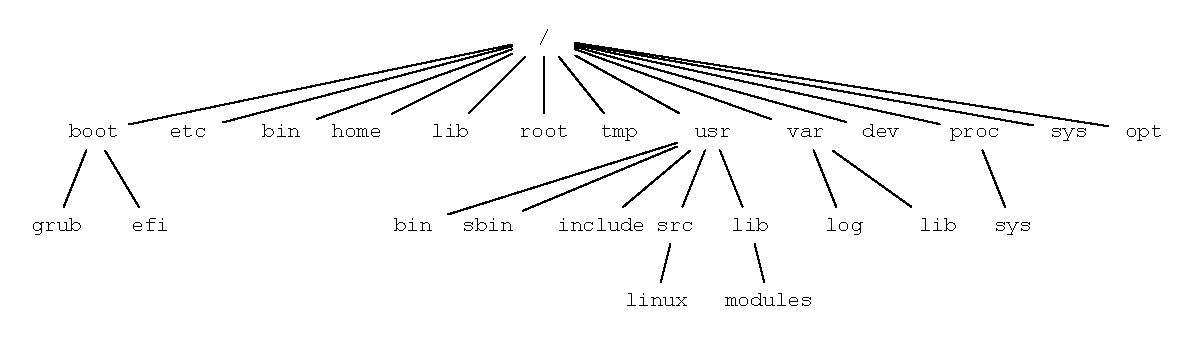
\includegraphics[scale=0.6]{figures/fs-tree.pdf}
	\centering
	\caption{The main directories in the root filesystem}
	\label{fig:fs-tree}
\end{figure}

\textbf{XXX---need to decide much of the tree I should describe}.

\begin{itemize}
	\item \cf{/bin} -- a symbolic link to \cf{/usr/bin} which contains almost 1500 general purpose commands such as \cf{ls(1)} 
		and \cf{mkdir(1)}.
	\item \cf{/etc} -- system-wide configuration files and system databases. It used to be the dumping ground for 
		everything else thus the name "etc" (etcetera). 
	\item \cf{/boot} -- the Linux kernel image, \cf{initrd} (initial RAM disk, GRUB configuration and anything else that
		is needed to bootstrap the system.
	\item \cf{/dev} -- all of the devices in the system. More specifically, these are special files that are used to access
		Linux devices attached to the system. 
	\item \cf{/home} -- home directories for users.
	\item \cf{/lib} -- a symbolic link to \cf{/usr/lib}. This directory shared libraries.
	\item \cf{/lib/modules} -- all of the compiled kernel modules are located under this directory. The filesystem modules 
		are located under \cf{/lib/modules/<kernel version>/kernel/fs}.
	\item \cf{/root} -- the home directory for \cf{root}. It's separated from \cf{/home} since user data is often kept on a 
		separate filesystem which is mounted later in the boot process. At various times it may be necessary to boot
		to single user mode and for root to be able to login and diagnose issues. This occurs before general filesystems
		are mounted.
	\item \cf{/usr/src/linux} -- the Linux headers are here by default but not the source code. Installing the kernel
		source code can be done using Linux distribution-specific commands or you can downloaded a kernel
		of your choice from \cf{www.kernel.org}.  To build a Linux kernel you don't need to put the source code here. You
		can build and install the kernel as a general user. This will be discussed more in chapter \ref{disk-fs}.
	\item \cf{/proc} -- there are many interesting bits of information in \cf{/proc} that are related to
		file access and filesystems. We'll be exploring these in section \ref{procfs}.
	\item \cf{/sbin} -- a symbolic link to \cf{/usr/sbin}, this directory contains programs used to boot and administer the 
		system. Programs here are not typically used by general users.
	\item \cf{/tmp} -- used for storing temporary files. Once upon a time, these files were cleared each time the system
		was rebooted. Now it is cleared after a predefined number of days which differs per Linux distribution. Just never 
		assume that any files you place here will still be there after the next reboot. The \cf{/var/tmp} directory is
		similar but has a longer retention period.
	\item \cf{/var/log} -- holds system log files.
	\item \cf{XXX} -- \textbf{more? check when reading back again}
\end{itemize}

%%%%%%%%%%%%%%%%%%%%%%%%%%%%%%%%%%%%%%%%%%%%%%%%%%%%%%%%%%%%

\section{How Simple it Used to be}

In early versions of UNIX as well as Linux, a disk partitioning was very simple. There was a bootstrap block and the UNIX  filesystem. To go back and see how UNIX handled the boot process back in 1975, you can get hold of John Lyons' "\textit{A Commentary on the 6th Edition UNIX Operating System}" online. The source code is available on github at: 

\begin{table}[h]
\begin{tabular}{lcl}
\parbox[r]{0.5in}{ 
\includegraphics[scale=0.15]{figures/url.png}} & \parbox[l]{0.1in}{\arabic{urls}} & \parbox[l]{3in}{\cf{https://tinyurl.com/u36a2a3a}}
\end{tabular}
\end{table}
\stepcounter{urls}
% https://github.com/memnoth/unix-v6

\noindent
In the top-level \cf{README.md} you will find a link to Lions' book. I remember when I first got hold of John Lions' book and seeing all of the UNIX source code at just over 11,000 lines of code. At the time I was working on getting the \cf{truss(1)} utility (UNIX equivalent of \cf{strace(1)} running on the SVR4 subsystem on the Chorus microkernel at the time. It was about the same amount of code. Gulp! How things were much simpler back then.

Bootstrap was very simple. The initial boot loader was located firmware. Its goal was to load block 0 which contained a larger boot program. This boot program looked for and loaded \cf{/unix} to which it passes control. The superblock of the root filesystem was always stored in block 1. \textbf{did they really not have mountable filesystems? I thought I saw mount in there somewhere? Check}

Additional filesystems could be mounted - \textbf{XXX---walk through the code and see how it worked}

% https://web.cs.wpi.edu/~rek/DCS/D04/UnixFileSystems.html - old fs layout - need more accurate info

%%%%%%%%%%%%%%%%%%%%%%%%%%%%%%%%%%%%%%%%%%%%%%%%%%%%%%%%%%%%

\section{Filesystems, Disks and Partitions}\label{partitions}

Things to cover:

\begin{itemize}
	\item physical vs logical block sizes
	\item maximum file and filesystem sizes and how fs block size affects this
	\item block allocation vs extents
	\item perhaps show old single, double and triple extents to show how things have changed
	\item full fsck vs journaling
	\item partition highlights before describing in more details in next sections
\end{itemize}

Filesystem on-disk structures have become considerable more complicated in the last thirty years compared to early days of UNIX and Linux.

%-----------------------------------------------------------------------------------------------------------------------------------------------------------------------

\subsection{Filesystem On-disk Structure}

Disks are partitioned using different partitioning schemes which will be described soon but generally speaking, there can be multiple partitions within a single disk and each partition can contain a filesystem that can be mounted separately onto a directory in the Linux file hierarchy. Figure \ref{fig:basic-disk-layout} shows the basic components of a traditional filesystem.

\begin{figure}[h]
	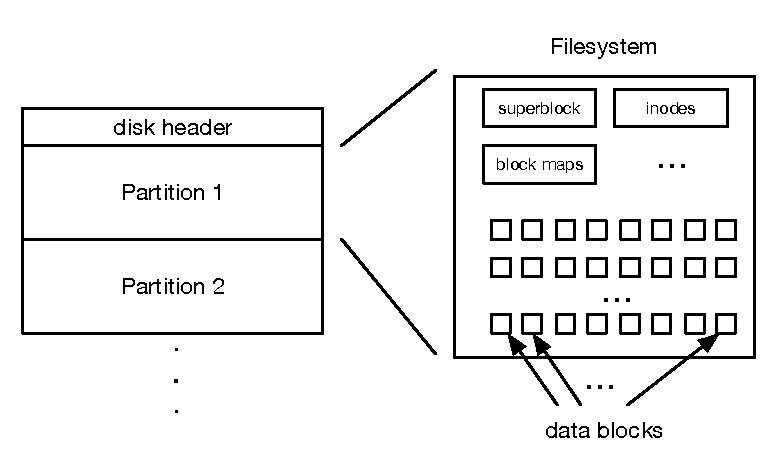
\includegraphics[scale=0.6]{figures/basic-disk-layout.pdf}
	\centering
	\caption{A disk partition with general filesystem disk structures}
	\label{fig:basic-disk-layout}
\end{figure}

\noindent
Todays filesystems are much more complicated and will described later in the book. However, this is the minimal set of data structures needed to create a fully functioning filesystem.

\begin{itemize}
	\item \textbf{superblock} -- the first structure that will be read from disk when the filesystem is mounted. It contains enough 
		information to locate the other structures needed to access files, allocate data blocks and so on. There may
		be multiple copies of the superblock to guard against disk errors. 
	\item \textbf{inode} -- a structure on disk that represents a file regardless of the file type. It contains file meta-data which 
		describes the file including type, size, owner and the location of the file's \textit{data blocks}. There may be
		a preallocated inode list or inodes may be allocated dynamically allowing for a larger number of files.
	\item \textbf{data blocks} -- contain actual data whether it be regular file data, directory entries or symbolic links.
	\item \textbf{block map} -- a data structure that indicates which blocks have been allocated. Data blocks are of fixed size and
		the size is chosen when the filesystem is created.
\end{itemize}

\noindent 
The filesystem on-disk structure has evolved considerably over time primarily to address resilience, performance, file and filesystem size but also to incorporate new features such as snapshots, file activity change logs and journaling capabilities.

%-----------------------------------------------------------------------------------------------------------------------------------------------------------------------

\subsection{Referencing Data Blocks From The Inode}

To help explain file and filesystem sizes and how they differ depending on the filesystem block size, consider figure \ref{fig:indirects} which shows the layout of a file in the ext2 filesystem. 

\begin{figure}[h]
	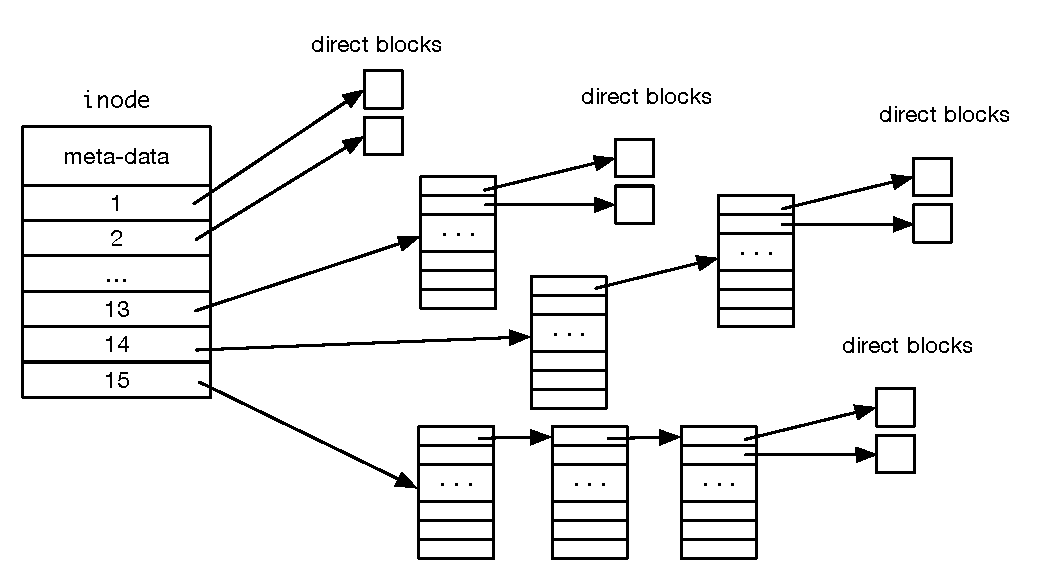
\includegraphics[scale=0.6]{figures/indirects.pdf}
	\centering
	\caption{The UFS on-disk structure for a file}
	\label{fig:indirects}
\end{figure}

\noindent
Inside the inode is meta-data about the file in addition to fifteen pointers that reference the file's data blocks either directly or indirectly. There are:

\begin{itemize}
	\item twelve direct pointers that points to blocks of actual data for the file.
	\item one single-indirect pointer that points to a block of pointers that then point to actual data blocks.
	\item one double-indirect pointer that points to a block of pointers that point to other blocks of pointers 
		that finally point to blocks of data for the file.
	\item one triple-indirect pointer that points to a block of pointers that point to other blocks of pointers 
		that point to other blocks of pointers that finally point to blocks of the file's data.
\end{itemize}

\noindent
The size of each block of data depends on the filesystem block size. Let's take ext4 as an example. It has four different filesystem block sizes that are specified when the filesystem is made. This means that each data block can range from 1 KB to 8 KB resulting in very different file sizes depending on the block size chosen as show in table \textbf{XXX---reverse direction and color}

\begin{table}
\centering
\begin{tabular}{|c|c|c|}
\hline
block size&maximum filesystem size&maximum file size\\
\hline
1 KiB&16 GB&4 TB\\
2 KiB&256 GB&8 TB\\
4 KiB&2 TB&16 TB\\
8 KiB&2 TB&32 TB\\
\hline
\end{tabular}
\end{table}

\noindent
xxx

%-----------------------------------------------------------------------------------------------------------------------------------------------------------------------

\subsection{Full Filesystem Check vs Journaling}

When a filesystem is mounted for read/write access, it is generally marked \textit{dirty} indicating that changes are occurring. This has traditionally been done by setting a flag in the superblock. When the filesystem is a unmounted it is marked \textit{clean}. If the system crashes between these two events, the filesystem could be in an inconsistent state. For example, when creating a file, there are several structures on disk that need to be modified. If the system crashes in the middle of these operations, the filesystem needs to undo those operations the operations that it performed to make the filesystem structurally intact again. To bring the filesystem back to being structurally intact, a \cf{fsck} (filesystem check) is needed. This is performed prior to the filesystem being mounted again, typically as part of the book process. This is a process that can take a very long time typically dependent on the number of files in the file system. Many hours there's not unlikely.

This is where \textit{filesystem journaling} comes into play. First introduced in the VERITAS VxFS filesystem and now available in several (name them???) Linux filesystems, journaling involves writing upcoming structural changes to an \textit{intent log} before changing the actual on-disk structures themselves. If the system crashes, log replay is performed which takes a very short amount of time. Journaling will be described in more detail in section TBD.

%-----------------------------------------------------------------------------------------------------------------------------------------------------------------------

\subsection{Disk Partitioning}

This is another topic to which a whole chapter could be dedicated but it really beyond the scope of this book. But partitioning affects many things from bootstrap to choosing how to layout filesystem. Whether using disks directly or using logical volume managers to manage the disks for you, it's important to spend some time explaining how disks are partitioned.

The two primary gains of GPT over MBR are:

\begin{enumerate}
	\item Large partitions, more that 2 TB
	\item Unlimited number of primary partitions
\end{enumerate}

%-----------------------------------------------------------------------------------------------------------------------------------------------------------------------

\subsection{The GPT Disk Format}

This section highlights the GPT format and shows how filesystems are stored within GPT partitions. A GPT-partitioned disk is shown in figure \ref{fig:gpt} with a hypothetical filesystem shown on partition 1. 

\begin{figure}
	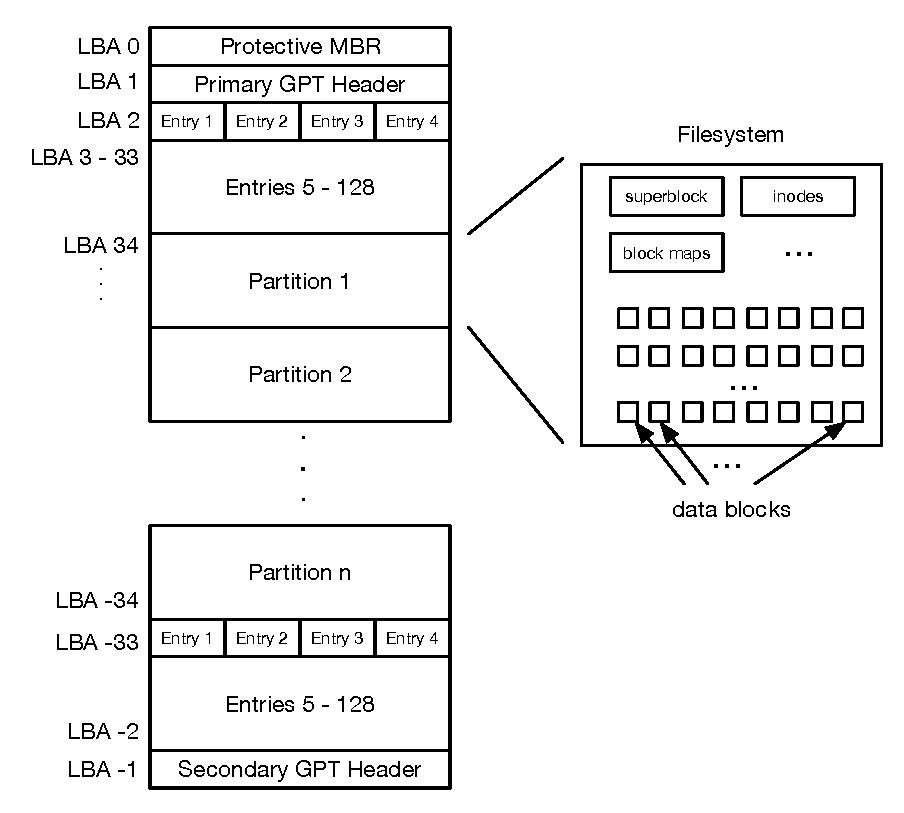
\includegraphics[scale=0.6]{figures/gpt.pdf}
	\centering
	\caption{GPT partitioned disk and filesystem within a partition}
	\label{fig:gpt}
\end{figure}

For each partition that contains a filesystem, the filesystem will \textit{manage} the layout of the partition. There will be filesystem meta-data which includes information about the filesystem itself (superblock), structures for allocated files (usually inode structures) and other information such as tracking data blocks which have been allocated. The meta-data only takes up a relatively small amount of space and the rest of the partition is open for storing file data. The exception to this is the RAM-based filesystems that have been used in Linux since early days (\textbf{XXX---day 1?}) which will be discussed in section \ref{ramfs}.

Some points to note about the figure:

\begin{itemize}
	\item LBA stands for Logical Block Addressing.  Each block is 512 bytes.
	\item There are two copies of the GPT header, one at the start of the disk and one in the last block (LBA - 1).
	\item The partition table starts at LBA 2 and there are up to 128 partitions. Each partition table entry is 128 bytes.
	\item \textit{Usable} partitions start with partition 1 and LBA 34. 
\end{itemize}

\noindent
blah 

%%%%%%%%%%%%%%%%%%%%%%%%%%%%%%%%%%%%%%%%%%%%%%%%%%%%%%%%%%%%

\subsection{Logical Volumes Managment}

For developmental or experimental purposes, you will likely only need one or two disk. On my Ubuntu VMs, I have one disk for Ubuntu itself and another small disk which I partition and use for storing filesystems that I'm developing or playing with. You can also create loopback devices and place filesystems on there.

In the real world, the amount of data that organizations need to store well exceeds the size of individual disks so managing hundreds, thousands or tens of thousands of individual disks makes no sense. This is where \textit{logical volume management} comes into play. Of course, most organizations will unlikely deal with disks themselves but rather get their storage management solutions from one of the many storage vendors on the market today. Each of these vendors will package many disks inside the storage arrays using logical volume manager technology for which some of the technology will be hidden from the customer.

Before working on the VERITAS filesystem VxFS, my first introduction to VERITAS came when I ported their volume manager VxVM to SVR4 UNIX running on the Chorus microkernel back in the early 1990s. VxVM was ported to many operating systems throughout the 90s, became a standard part of Microsoft Windows several during that time and my colleagues and friends ported it to Linux at the same time my team was porting VxFS to Linux.

%-----------------------------------------------------------------------------------------------------------------------------------------------------------------------

\subsection{Advantages of Logical Volume Management}

There are many advantages of logical volume management (LVM) and perhaps top of the list is ease of management. Rather than partitioning large numbers of disks and having to management them yourself, just give the disks to the volume manager and create new volumes as needed and not have them restricted by the size of the disk partitions.

Some have argued that LVM just adds another layer to the storage stack and has some performance overheard. However, the actual performance reduction is very minor and offset by the advantages that LVM offers. But as volumes are created and overlap on the underlying shared storage, fragmentation can become an issue leading to potential performance issues. These are all issues that the LVM vendors such as VERITAS addressed in their products.

Since this section is just highlighting the area of logical volume management, here are some of the major advantages:

\begin{itemize}
	\item Ease of management compared to handling large numbers of disks / partitions.
	\item Avoid the limits imposed by physical disk sizes / partitions.
	\item Increase or decrease the size of volumes and therefore the size of the filesystems that reside on them. For example,
		when extending the size of a filesystem, the operation can be done in five steps using Linux LVM. 
		Of course, if space is already available in the existing volume group, the first two steps can be omitted. 
	\begin{enumerate}
			\item Add new storage
			\item Create a new physical volume
			\item Extend the volume group to include the new physical volume
			\item Extend the Logical Volume 
			\item Extend the filesystem
		\end{enumerate}
	\item Performance gains through the use of \textit{striping}, where data is in a logical volume is spread across multiple
		devices and performance is increased since reads/writes happen in parallel.
	\item Redundancy through mirroring, where the same data is copied to two or more physical devices. If one of the devices
		dies or goes offline for some reason, the data on the other devices can still be accessed.
	\item Other RAID (Redundant Array of Inexpensive Disks) levels including RAID4 and RAID 5 which provide parity,
		a common way of detecting errors in a storage system. 
	\item Snapshots for backup purposes independent of the filesystem type. Not all filesystems support snapshot mechanisms.
\end{itemize}

\noindent 
Generally speaking, logical volume management allows users to build enterprise-level capabilities with inexpensive disks. Most modern storage systems have all of these capabilities built-in but come at additional cost.

%-----------------------------------------------------------------------------------------------------------------------------------------------------------------------

\subsection{Linux LVM}

Heinz Mauelshagen wrote the original LVM code back in 1998, taking its primary design guidelines from the HP-UX's volume manager, which was actually the VERITAS volume manager VxVM. I remember going to a small Linux conference in Frankfurt, Germany around that time that Heinz hosted. Version 1 of LVM was introduced into the 2.4 kernel series. LVM version 2 (or just LVM2) became available in kernel versions 2.6.9 and above.

Around this time, logical volume management was extremely popular with many organizations managing large numbers of disks which is problematic for many reasons. This popularity somewhat declined in subsequent years with newer storage arrays that had all of this functionality built-in. But in those cases, the logical volume management component simply shifted from the server or VM running Linux to the storage array itself. Take most IaaS (Infrastructure As A Service) solutions in the cloud. All of these capabilities are built in to the storage fabric and Linux just sees simple partitions. The same is true of most hypervisor solutions for which thin provisioning is an important capability but also hidden from the Linux operating system. Thing provisioning is a technique where storage blocks are only allocated as needed. It may look like you have 40 GB drive but if there is only 20 GB of data in used, only 20 GB of data is allocated from the underlying fabric.

Use of LVM still continues to this day. Some Linux distributions use LVM to configure the root device. For example, the Ubuntu VMs I am are partitioned as follows:

\begin{lstlisting}
$ [*\bfseries df -h*]
Filesystem                  Size Used Avail Use% Mounted on
tmpfs                       392M 1.2M  391M   1% /run
/dev/mapper/ubuntu--vg-...v  30G  21G  7.5G  74% /
tmpfs                       2.0G    0  2.0G   0% /dev/shm
tmpfs                       5.0M    0  5.0M   0% /run/lock
/dev/sda2                   2.0G 269M  1.6G  15% /boot
/dev/sda1                   1.1G 6.1M  1.1G   1% /boot/efi
tmpfs                       392M 4.0K  392M   1% /run/user/1000
\end{lstlisting}

\noindent
\textbf{XXX -- at some point, install other distros and see if they use LVM by default}

%-----------------------------------------------------------------------------------------------------------------------------------------------------------------------

\subsection{LVM Concepts}

LVM functions by layering abstractions on top of physical storage devices. The basic layers that LVM uses, starting with the most primitive, are shown in figure \ref{fig:LVM}:

\begin{figure}[h]
	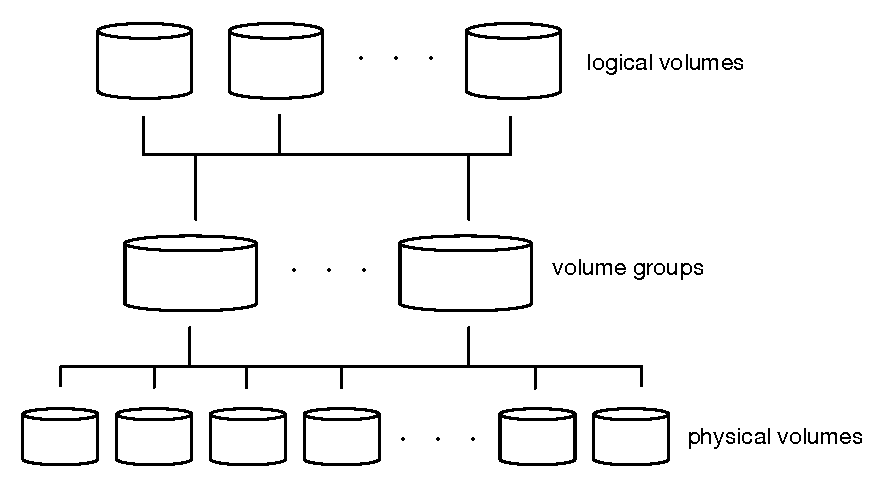
\includegraphics[scale=0.6]{figures/LVM.pdf}
	\centering
	\caption{LVM Architecture}
	\label{fig:LVM}
\end{figure}

\begin{itemize}
	\item \textbf{Physical Volumes} (PVs) -- LVM uses physical block devices such as hard disk drives, solid-state drives or 
		partitions. An LVM label is written near the start of the disk to correctly identify the device. This is particularly important
		when physical devices are removed/added since device names can change. The LVM utility prefix for physical volumes
		is \cf{pv}.
	\item \textbf{Volume Groups} (VGs) -- LVM combines physical volumes into storage pools called volume groups. You can
		think of them as very large disks. This concept was introduced in volume managers many years ago to allow for
		filesystems or raw volumes to be much bigger than the largest available disks at the time. The same is still true
		today. The LVM utility prefix for volume groups is \cf{vg}. 
	\item \textbf{Logical Volumes} (LVs) --  A volume group can be sliced up into any number of logical volumes. Logical volumes 
		are functionally equivalent to partitions on a physical disk in that you create a filesystem on top of a logical volume.
		However, they have much more flexibility. Logical volumes are the primary component that users and applications 
		will interact with. The LVM utility prefix for logical volumes is \cf{lg}. 
\end{itemize}

\noindent
Using the Ubuntu disk layout shown above, the following commands show the different LVM layers. First of all, here is the single physical volume which is constructed from a single disks \cf{/dev/sda3}:

\begin{lstlisting}   
$ [*\bfseries sudo pvdisplay*]
  --- Physical volume ---
  PV Name               /dev/sda3
  VG Name               ubuntu-vg
  PV Size               <60.95 GiB / not usable 3.00 MiB
  Allocatable           yes 
  PE Size               4.00 MiB
  Total PE              15602
  Free PE               7801
  Allocated PE          7801
  PV UUID               wpN3k3-OjXr-8FKN-CG0I-kf0B-hlK6-h0zXh9
\end{lstlisting}

\noindent
Next is the single volume group \cf{ubuntu-vg}:

\begin{lstlisting}   
$ [*\bfseries sudo vgdisplay*]
  --- Volume group ---
  VG Name               ubuntu-vg
  System ID             
  Format                lvm2
  Metadata Areas        1
  Metadata Sequence No  2
  VG Access             read/write
  VG Status             resizable
  MAX LV                0
  Cur LV                1
  Open LV               1
  Max PV                0
  Cur PV                1
  Act PV                1
  VG Size               <60.95 GiB
  PE Size               4.00 MiB
  Total PE              15602
  Alloc PE / Size       7801 / 30.47 GiB
  Free  PE / Size       7801 / 30.47 GiB
  VG UUID               CdWVPi-TAwA-7jtZ-iPFb-xq6k-ybeO-NKJNFY
\end{lstlisting}

\noindent
On top of this volume group there is a logical volume called \cf{ubuntu-lv}:

\begin{lstlisting}
$ [*\bfseries sudo lvdisplay*]
[sudo] password for spate: 
  --- Logical volume ---
  LV Path                /dev/ubuntu-vg/ubuntu-lv
  LV Name                ubuntu-lv
  VG Name                ubuntu-vg
  LV UUID                NXbsIa-999P-8QeO-aHJh-EdVU-jY2C-zOruGY
  LV Write Access        read/write
  LV Creation host, time ubuntu-server, 2023-04-19 09:13:27 +0000
  LV Status              available
  # open                 1
  LV Size                30.47 GiB
  Current LE             7801
  Segments               1
  Allocation             inherit
  Read ahead sectors     auto
  - currently set to     256
  Block device           253:0
\end{lstlisting}

\noindent
This is a very simple setup. If you want to play with LVM, you will need lots of disks and/or partitions. If you're operating in a virtualized world, that's very easy to do. You don't need to have large disks just to experiment.

%---------------------------------------------------------------------------------------------------------------------------------------------------------------------

\section{ZFS -- Builtin Volume Management}

The Z File System (ZFS) was created inside Sun Microsystems in 2001 by Bill Moore, Matthew Ahrens and Jeff Bonwick. It was designed to be the next generation file system for Sun Microsystems’ OpenSolaris following years of battles between Sun's UFS and the VERITAS filesystem VxFS. VxFS was much more feature rich and most of VERITAS' revenue came from Solaris, During this time Sun kept enhancing UFS mostly in the area of improving performance. This would be followed by an intense period at VERITAS to increase VxFS performance further.

In 2008, ZFS was ported to FreeBSD and we used it as part of the base OS at my second startup High Cloud Security. During the same year a port ZFS to Linux was initiated but has suffered due to the different licensing terms. ZFS is licensed under the Common Development and Distribution License (CDDL), which is incompatible with the GNU General Public License (GPL). Because of this, it cannot be included in the Linux kernel. To work around this problem ZFS if offered separately by some Linux distributions.

ZFS is a different filesystem altogether in that it includes builtin logical volume management.

Features include: \textbf{XXX -- need to look at this list, add more and get info from different sites}

\begin{itemize}
	\item Inline Data Compression -- xxx
	\item Send/Receive snapshots -- a \textit{snapshot} of a file system can be taken and this snapshot image can be sent 
		to a different server. This allows data from the original filesystem to be replicated for the purpose of 
		backing up data or enabling data migration to the cloud.
	\item Inline Data Deduplication -- xxx
	\item RAID-Z and Mirroring -- xx
	\item Hierarchical checksumming of all data and metadata -- xxx
	\item Automatic rollback of recent changes to the file system and data -- xxx
	\item Native handling of tiered storage and caching devices -- xxx
	\item Data integrity -- xxx
\end{itemize}

\noindent
Should you look at ZFS? The fact that it's not included directly in Linux distributions and may therefore have support issues, ZFS is a very feature-rich filesystem. Regardless of commercial use, it's worthy of study.

%%%%%%%%%%%%%%%%%%%%%%%%%%%%%%%%%%%%%%%%%%%%%%%%%%%%%%%%%%%%

\section{Filesystem Types Supported by Linux}

At the time of writing there are over 80 different filesystems supported by Linux. How many of them are actually used? 

It might be good to try and categorize them???

\begin{quote}
Wkipedia has a good page that i should cover - https://en.wikipedia.org/List\_of\_file\_systems
\end{quote}

\begin{itemize}
	\item Disk file systems
	\item File systems with built-in fault-tolerance
	\item File systems optimized for flash memory, solid state media
	\item Record-oriented file systems
	\item Shared-disk file systems
	\item Distributed file systems
	\item Distributed fault-tolerant file systems
	\item Distributed parallel file systems
	\item Distributed parallel fault-tolerant file systems
	\item Peer-to-peer file systems
	\item Special-purpose file systems
	\item Pseudo file systems
	\item Encrypted file systems --- this list excludes commercial solutions such as SecFS from 
		Thales (formerly Vormetric) and their FUSE-based encryption solution.
\end{itemize}

\noindent
In this book, we'll be covering pseudo filesystems as well as disk-based and FUSE-based filesystems. We'll also cover encrypted filesystems as part of looking at implementing a FUSE-based filesystem. 

%%%%%%%%%%%%%%%%%%%%%%%%%%%%%%%%%%%%%%%%%%%%%%%%%%%%%%%%%%%%

\section{How Many Filesystems are Actually Used?}

Although there are over 80 filesystems in the Linux kernel source and many FUSE and other filesystems elsewhere on the web, how many are actually used? Let's start with the root filesystem for the major Linux distributions today:

\begin{itemize}
	\item Ubuntu / Debian --- ext4
	\item Fedora --- btrfs 
	\item CentOS --- XFS
	\item RHEL --- XFS - was ext4 up to RHEL 6.0
	\item OpenSuSE --- btrfs
	\item SLES --- XFS
	\item Android --- ext4 or one of the flash-based filesystems such as YAFFS2. 
\end{itemize}

\noindent
Generally speaking, either \cf{ext4} or \cf{btrfs} are chosen as the default root filesystem apart from the server versions of Linux which use XFS. There are many opinions about whether \cf{btrfs} will replace \cf{ext4} in desktop or general non-server environments. It certainly has a lot more features but stability and performance are raised as concerns (at the time of writing). Generally speaking, I would advise to go with the default filesystem for a specific distribution unless you have specific needs or want to experiment with a different filesystem. The default filesystem will be the one most tested in the largest number of environments and situations. Since Ubuntu is the most widely used Linux distribution with the exception of mobile devices and Android devices either use ext4 or have been migrating towards \cf{ext4}, it could be argued that \cf{ext4} is the most widely used filesystem on Linux devices today.

On a default Ubuntu VM I have the following on the VMs I'm using when writing this book:

\begin{lstlisting}
$ [*\bfseries cat /proc/filesystems*]
nodev	sysfs
nodev	tmpfs
...
ext3
ext2
ext4
...
$ [*\bfseries cat /proc/filesystems | wc -l*]
33
$ [*\bfseries cat /proc/filesystems | grep nodev | wc -l*]
26
$ [*\bfseries mount | wc -l*]
32
\end{lstlisting}

\noindent
So interestingly enough, out of the 33 filesystem modules currently loaded, 26 of them are pseudo filesystems. By default, ext4 is the root filesystem on Ubuntu. Furthermore, running \cf{mount(1)}, there are 32 mounted filesystems. Here are the 7 that are displayed by \cf{df(1)}:

\begin{lstlisting}
$ [*\bfseries df -T*]
Filesystem  Type 1K-blocks    Used Available Use% Mounted on
tmpfs       tmpfs   400608    1340    399268   1% /run
/dev/map... ext4  39396672 1408380  25954836  31% /
tmpfs       tmpfs  2003028       0   2003028   0% /dev/shm                            
tmpfs       tmpfs     5120       0      5120   0% /run/lock
/dev/vda2   ext4   1992552  505692   1365620  28% /boot
/dev/vda1   vfat   1098628    5220   1093408   1% /boot/efi
tmpfs       tmpfs   400604       4    400600   1% /run/user/1000
\end{lstlisting}

\noindent
There are 3 FUSE filesystems that are registered which are not installed by default. They're available on my VM as I had been developing FUSE-based filesystems at the time of writing.

If you want the default filesystems that operating systems have used going back to 1968, the Wikipedia page (https://en.wikipedia.org/wiki/List\_of\_default\_file\_systems) provides an insight. It's not a very complete list as it excludes the various UNIX versions over the years as well as mainframe operating systems. For an historical perspective on Linux variants, it's more interesting. 

\noindent 
Another way to view mounted filesystems is to call the \cf{findmnt(8)} command, the output of which is shown in figure \ref{fig:findmnt}.

\begin{figure}
	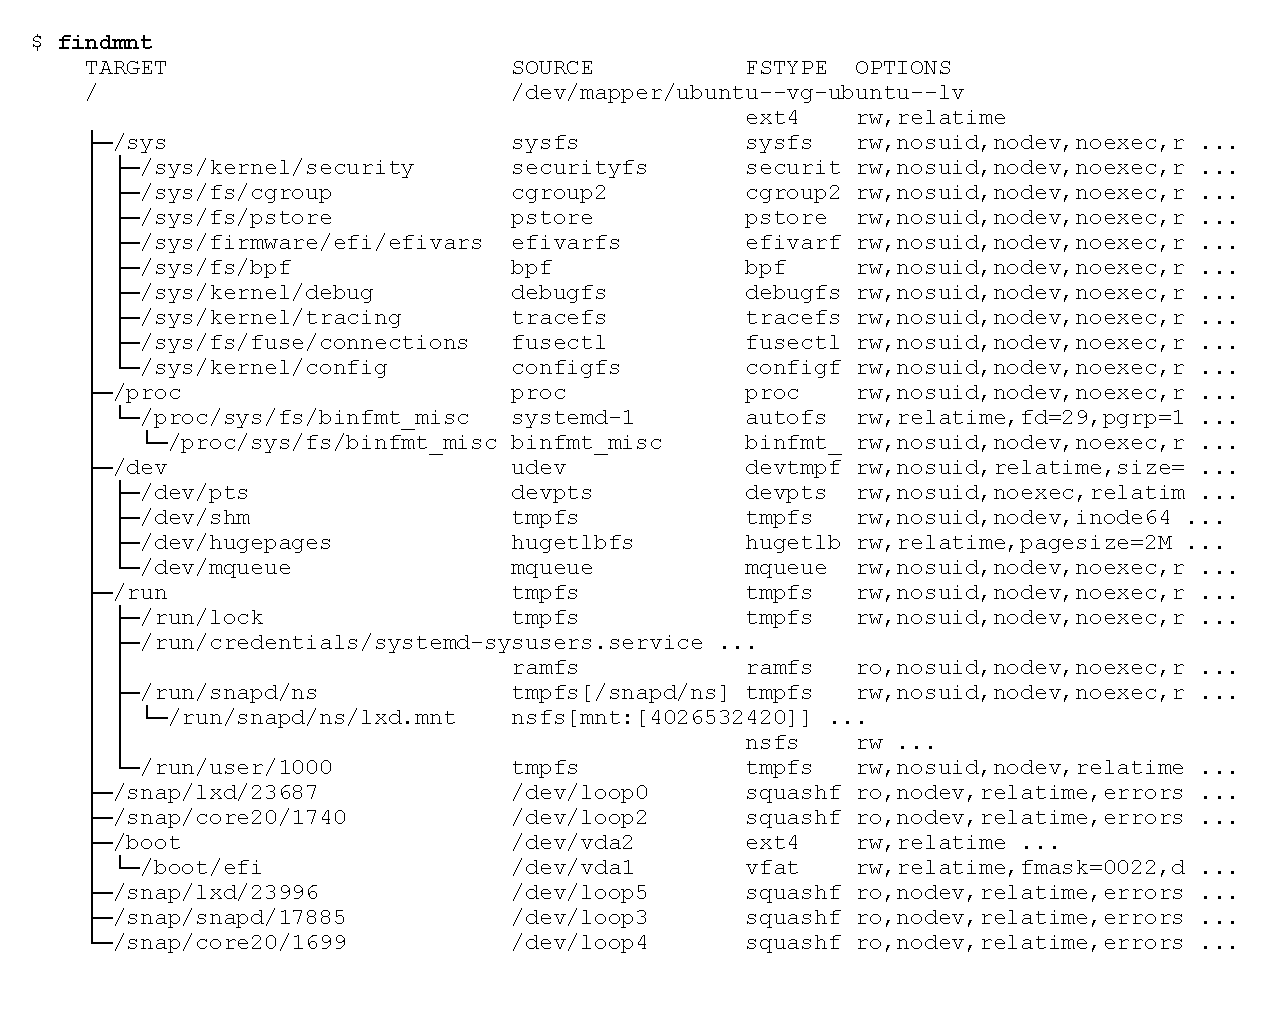
\includegraphics[scale=0.6]{figures/findmnt.pdf}
	\centering
	\caption{The \cf{findmnt(8)} command displays all mounted filesystems}
	\label{fig:findmnt}
\end{figure}

\noindent
You can also cat \cf{/proc/mounts} and get the same information but in a less pretty form.

%%%%%%%%%%%%%%%%%%%%%%%%%%%%%%%%%%%%%%%%%%%%%%%%%%%%%%%%%%%%

\section{Comparing the Main Filesystem Types}

% https://linuxiac.com/linux-file-system-types-explained-which-one-should-you-use/

Add some info about number of LOC for smallest, largest, most common etc

\begin{table}[h]
\begin{center}
\begin{tabular}{|p{0.2\textwidth}|m{0.4\textwidth}|}
\hline
\rowcolor[gray]{.93}\bf{Filesystem}&\bf{Lines Of Code (LOC)}\\
\hline
ext2 & 9,672\\
\hline
ext4 & 62,677\\
\hline
xfs & 70,520\\
\hline
btrfs & 146,306\\
\hline
\end{tabular}
\label{table:fs-loc}
\caption{\small Popular filesystems and their LOC in the kernel}
\end{center}
\end{table}

%-----------------------------------------------------------------------------------------------------------------------------------------------------------------------

\subsection{The ext2/3/4 Filesystems}

\textbf{XXX---still some plagerism particularly around bullet points}

The first Linux filesystem mirrored the filesystem structure from Andrew Tanenbaum's operating system MINIX. This had a number of limitations such as 14 character filenames and a maximum filesystem size of 64 MB. This filesystem was soon replaced with ext, the extended filesystem, which was added to Linux kernel version 0.96c in April 1992. It could handle file systems up to 2 GB and file names of up to 255 characters. But it had its own problems in that there was no support for separate timestamps for file access, inode modification, and data modification (atime, mtime and ctime).

To continue to make improvements, work on two new filesystems started in early 1993 for Linux kernel 0.99. These filesystems were xiafs developed by Frank Xia and the second extended file system (ext2) developed by R\'emy Card. Xiafs was still modeled around the MINIX filesystem while ext2 got its inspiration from the BSD filesystem UFS. Xiafs was less powerful and had less functionality than ext2 so over time, it was phased out. You won't find the source code in the Linux kernel any more while ext2 is still there (\cf{fs/ext2}).

The main features of ext2 or points to highlight are:

\begin{itemize}
	\item Block sizes of 1, 2, 4 and 8 KB.
	\item A maximum individual file size can be from 16 GB to 2 TB depending on the filesystem block size.
	\item A maximum file system size ranges from 4 TB to 32 TB depending on block size.
	\item Compression and decompression of files with the \cf{e2compr} patch.
	\item Since ext2 does not have journaling capabilities, if the system crashes, a full \cf{fsck} needs to be run. \textbf{TBC}
	\item On flash drives and USB drives, ext2 is recommended to reduce the overhead of journaling. \textbf{TBC}
\end{itemize}

\noindent
Ext3, or the third extended file system was introduced by Stephen Tweedie in 2001. It was merged into kernel version 2.4.15 in XXX. It had the following features:

\begin{itemize}
	\item Full filesystem journaling reducing the need for a full \cf{fsck} if the system crashes.
	\item Journaling has a dedicated area in the file system, where all the changes are tracked. When the system crashes, the 	\item possibility of file system corruption is less because of journaling.
	\item Maximum file size of 16 GB to 2 TB depending on block size.
	\item Filesystem between 2 TB to 32 TB depending on block size.
	\item You can convert a ext2 file system to ext3 file system directly (without backup/restore).
\end{itemize}

\noindent
There are three types of journaling available in ext3 file system.

\begin{itemize}
	\item Journal -- Metadata and content are saved in the journal.
	\item Ordered -- Only metadata is saved in the journal. Metadata are journaled only after writing the 
		content to disk. This is the default.
	\item Writeback -- Only metadata is saved in the journal. Metadata might be journaled either before or after 
		the content is written to the disk.
\end{itemize}

\noindent
The ext3 filesystem source code is no longer in the Linux kernel.

In June of 2006, Ted Ts'o, who was one of the the principal developers of ext3, announced ext4, the fourth extended file system. , The stable version was merged in the Linux kernel version 2.6.28 in October of 2008. He also stated that that although ext4 has improved features and is much faster than ext3, "\textit{it is not a major advance, it uses old technology, and is a stop-gap}". His belief is that btrfs is the better direction, because "\textit{it offers improvements in scalability, reliability, and ease of management}".

Ext4 has the following enhancements over ext3:

\begin{itemize}
	\item Supports huge individual file size and overall file system size.
	\item Maximum file size can be from 16 GB to 16 TB depending on the block size.
	\item Maximum file system size of 1 EB (exabyte). Note that 1 EB = 1024 PB (petabytes). 1 PB = 1024 TB (terabytes).
	\item Directories have a maximum of 64,000 subdirectories (this was increased from 32,000 in ext3)
	\item Several other new features are introduced in ext4: multi-block allocation, delayed allocation, 
		journal checksum. fast fsck, etc. All you need to know is that these new features have improved the 
		performance and reliability of the filesystem when compared to ext3.
	\item In ext4, you also have the option of turning the journaling feature “off”.
\end{itemize}

\noindent
XXX - what to write here depends on volume 1/2 vs a single book.

%-----------------------------------------------------------------------------------------------------------------------------------------------------------------------

\subsection{The XFS Filesystems}

XXX

Around the time we started the port of the VERITAS filesystem to Linux (late 1999), SGI were about to start porting their filesystem XFS. Soon after, both companies put out a press statement stating that the two companies had a joint project to bring a new, journaling filesystem to Linux. Since I was leading the effort at VERITAS I was surprised to see this news since I knew nothing of it. We quickly arranged a meeting between the two engineering teams (we were less than a mile apart) and all surprised that none of us ever knew anything about the press release. A quick marketing effort for some reason that none of us ever understood but we did stay in touch and shared our own experiences of porting what were likely, the two most feature rich commercial filesystems of the day.

\begin{itemize}
	\item Journaling -- 
	\item Allocation groups -- 
	\item Extent-based allocation -- 
	\item Striped allocation -- 
	\item A wide variety of block sizes -- from 512 bytes and 64 KB XXX
	\item Delayed allocation -- 
	\item Extended attributes - multiple data streams for files - hmm!
	\item Snapshots -- 
	\item On-line filesystem grow -- 
\end{itemize}

\noindent
XXX

%-----------------------------------------------------------------------------------------------------------------------------------------------------------------------

\subsection{The btrfs Filesystems}

% https://www.geeksforgeeks.org/how-to-create-btrfs-filesystem-in-linux-and-its-features/

Btrfs development began at Oracle in 2007. Btrfs is the next-generation general-purpose Linux file system that offers unique features like advanced integrated device management, scalability, and reliability. It is licensed under the GPL and open for contribution from anyone. There are different ways to pronounce the filesystem, including "Better FS”, “B-tree FS” and “Butter FS". Or just spell it out letter by letter. It was merged into the mainline Linux kernel in 2009 and first appeared in the Linux 2.6.29 release.

Goals

\begin{quote}
\textit{to let [Linux] scale for the storage that will be available. Scaling is not just about addressing the storage but also means being able to administer and to manage it with a clean interface that lets people see what's being used and makes it more reliable.}
\end{quote}

Although btrfs was included as a "technology preview" in Red Hat Enterprise Linux versions 6 and 7, it was removed in RHEL 8 in 2018. However, Fedora continued to offer it. \textbf{XXX---need to follow up on this one}. Looks like Red Hat have several XFS developers working for them.

The main features of btrfs are:

\begin{enumerate}
	\item \textbf{Extent-based allocation} -- earlier in the chapter, traditional disk layouts were described where blocks 
		are allocated to a file as direct, indirect, double indirect or triple indirects. In past times when files were not the 
		huge sizes that can be seen today, this was adequate. Extent based allocation was introduced in VxFS and XFS.
		In this scheme, variable size extents are allocated to a file. Take the case of a database. If the size of the database
		is known upfront and, let's say, that it's going to be 1 TB, why not have a single extent of 1 TB. This simplifies the
		inode structure and guarantees that all the data is contiguous on disk getting the best in terms of performance.
	\item Checksums -- 
	\item Cloning -- 
	\item Self-healing -- 
	\item Deduplication -- 
	\item Compression -- 
	\item Snapshots -- XXX. There is an example of using btrfs snapshots in section \ref{btrfs-snapshots}.
	\item Quota groups --
	\item File cloning -- 
	\item In-place conversation --
	\item Union mounting / seed devices -- 
	\item Online defragmentation, volume growth, and shrinking -- 
	\item Ability to handle swap files and swap partitions --
\end{enumerate}

\noindent
xxx

\subsection{The Flash??? Filesystems}

XXX - yaffs2 etc? F2FS 

\subsection{Stratis - RHEL???}

Wrong place but need to cover it.

% https://access.redhat.com/discussions/3138231 - see comments

%%%%%%%%%%%%%%%%%%%%%%%%%%%%%%%%%%%%%%%%%%%%%%%%%%%%%%%%%%%%

\section{Kernel or Userspace?}

Implementing a kernel-based filesystem is not trivial. I've worked on filesystem development for UNIX SVR3, SVR4, SCO UNIX, HP-UX, UnixWare, Solaris, Linux and various UNIX subsystems built on top of the Chorus microkernel. I actually started my filesystem career working on RFS back in the late 1980s. Debugging filesystems in the kernel is not easy. I've enjoyed using source level debuggers on HP-UX and Linux (through \cf{gdb} / \cf{kgdb}) but have also been stuck working at assembler level a lot and even had the pleasure (pain?) of working on debugging Solaris filesystems in \cf{adb} (yes, all in assembler) on Sparc systems with their peculiar register windows and lack of developer trust in arguments displayed in a stack trace.

But if you want performance, you'll be using one of the disk-based filesystems running on top of a high-performance storage system. \textbf{raw vs XXX}

In many cases, performance is not critical. For example, for personal use, I keep all of my source code files on my Mac where they're backed up and use SSHFS, which is a user-space filesystem developed using FUSE. Performance is not critical and usability wins the day. \textbf{XXX---expand on this}.

\textbf{does this section really belong here?}

%%%%%%%%%%%%%%%%%%%%%%%%%%%%%%%%%%%%%%%%%%%%%%%%%%%%%%%%%%%%

\section{Pseudo Filesystems}

A filesystem comprises a number of files which can be different types such as regular files or directories. In most cases, we deal with physical filesystems where these files are permanently stored. A pseudo filesystem on the other hand does not contain permanent storage. They are constructed as the kernel initializes and destroyed when the kernel shuts down.

The 3 well-known pseudo filesystems on Linux are proc (also called the /proc filesystem) which is mounted on \cf{/proc}, ramfs (\textbf{image when loading - come back to this}) and the sysfs filesystem which is mounted on \cf{/sys}. 

devfs), or a middle point such as Linux devtmpfs ???

Which pseudo filesystems are generally used? In my Ubuntu server VM, I've installed FUSE (which has 3 registered filesystems) but in addition to these, there are another 23 registered pseudo filesystems:

\begin{lstlisting}
$ [*\bfseries cat /proc/filesystems | grep nodev*]
nodev   sysfs
nodev   tmpfs
nodev   bdev
nodev   proc
nodev   cgroup
nodev   cgroup2
nodev   cpuset
nodev   devtmpfs
nodev   configfs
nodev   debugfs
nodev   tracefs
nodev   securityfs
nodev   sockfs
nodev   bpf
nodev   pipefs
nodev   ramfs
nodev   hugetlbfs
nodev   devpts
nodev   ecryptfs
nodev   fuse
nodev   fusectl
nodev   efivarfs
nodev   mqueue
nodev   pstore
nodev   autofs
nodev   binfmt_misc
\end{lstlisting}

\noindent
\textbf{XXX---need to think about how much to say here or whether we cover 1 or more in the kernel chapter}

%-----------------------------------------------------------------------------------------------------------------------------------------------------------------------

\subsection{The proc Filesystem}\label{procfs}

One filesystem that we will explore here is the proc pseudo filesystem (mounted on \cf{/proc} and also sometimes called the /proc filesystem) which contains a wealth of information about running process and a lot more information about the running system. It also provides the means through which different kernel parameters can be changed. There are close to 17,000 lines of code in the proc filesystem.

\begin{figure}[h]
	
\includegraphics[scale=0.95]{src-xref/procfs.pdf}
\end{figure}

The proc filesystem can be traced all the way back to UNIX 8th Edition and was first described in the 1984 USENIX paper "\textit{Processes as Files}":

\begin{table}[h]
\begin{tabular}{lcl}
\parbox[r]{0.5in}{ 
\includegraphics[scale=0.15]{figures/url.png}} & \parbox[l]{0.1in}{\arabic{urls}} & \parbox[l]{3in}{\cf{https://tinyurl.com/mvmb6nnj}}
\end{tabular}
\end{table}
\stepcounter{urls}
% https://lucasvr.gobolinux.org/etc/Killian84-Procfs-USENIX.pdf

The proc filesystem was then further developed as a collaboration between Sun Microsystems and AT\&T Bell Labs in the early 1990s for SVR4 UNIX and Solaris . Oddly enough, it actually began as a replacement for the \cf{ptrace(2)} system call which was the primary interface for debugging applications. Another goal was to replace ioctl(2) calls with standard \cf{read(2)} and \cf{write(2)} system calls which are better suited to network access. Commands such as \cf{ps(1)} and \cf{truss(1)} (UNIX version of \cf{strace(1)} were rewritten to use \cf{/proc}. I fully recommending reading the old USENIX paper.

\begin{table}[h]
\begin{tabular}{lcl}
\parbox[r]{0.5in}{ 
\includegraphics[scale=0.15]{figures/url.png}} & \parbox[l]{0.1in}{\arabic{urls}} & \parbox[l]{3in}{\cf{https://tinyurl.com/4wpmth6u}}
\end{tabular}
\end{table}
\stepcounter{urls}
% https://www.usenix.org/sites/default/files/usenix_winter91_faulkner.pdf

The proc filesystem was introduced in to Linux in 1992. Processes are described by looking at \cf{/proc/PID} where \cf{PID} is the process ID. FIgure \ref{fig:ls-proc} shows what's in \cf{proc} on my Ubuntu VM. As you can see, there is a lot more  in there other than just process-related information.

\begin{figure}
	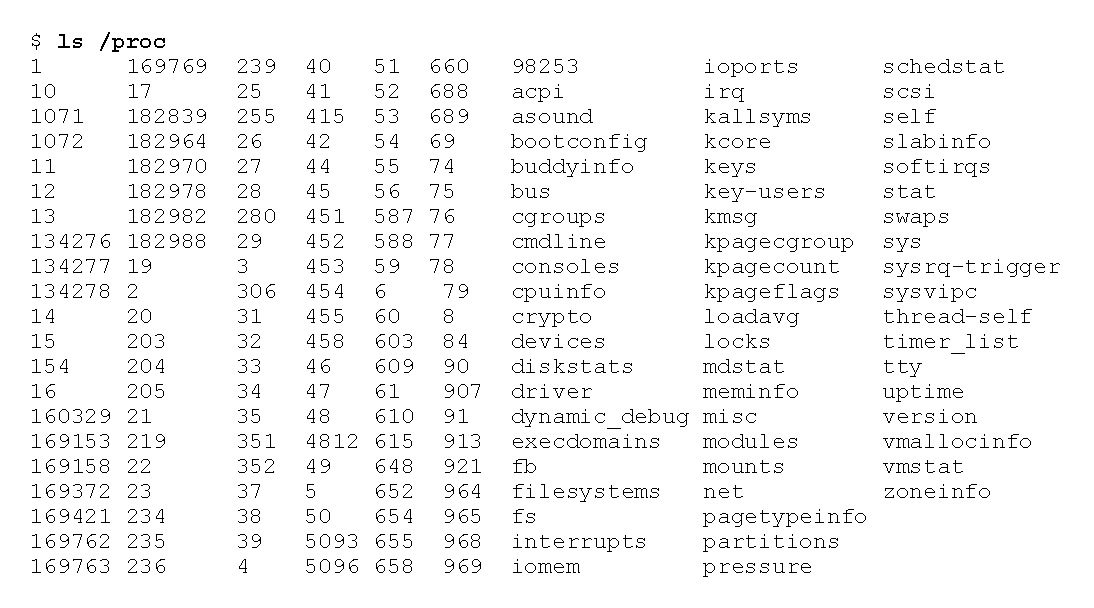
\includegraphics[scale=0.68]{figures/ls-proc.pdf}
	\centering
	\caption{The contents of \cf{/proc} on Ubuntu}
	\label{fig:ls-proc}
\end{figure}

For a process to get information about itself it can look under \cf{/proc/self}. Let's do a little exploring from the shell.

\begin{lstlisting}
$ [*\bfseries cd /proc/self*]
$ [*\bfseries cat cmdline*]
-bash           # actually doesn't add a newline
$ [*\bfseries ls -l exe*]
lrwxrwxrwx 1 spate spate 0 Nov 29 06:20 exe -> /usr/bin/bash
\end{lstlisting}

Need to look at following for /proc/self/fds/255 - %https://askubuntu.com/questions/866712/what-are-these-auxiliary-file-descriptors/866722#866722

Good site - %https://tldp.org/LDP/Linux-Filesystem-Hierarchy/html/proc.html

%-----------------------------------------------------------------------------------------------------------------------------------------------------------------------

\subsection{The Ramfs Filesystem}\label{ramfs}

One pseudo filesystem that is always used and part of the boot process is Ramfs, a RAM-based filesystem. XXX need to get info on how it's built.

The code for Ramfs is very small at only just over 600 lines of code.  Since it's so small, the ramfs module is always loaded

\begin{table}[h]
\begin{tabular}{ll}
\parbox[l]{0.6in}{
\includegraphics[scale=0.8]{figures/src-xref.pdf}} & \parbox[l]{4in}{\small{All of the Ramfs code can be found in \cf{fs/ramfs}.}}
\end{tabular}
\end{table}

\noindent
There really isn't a lot too the code and the filesystem relies mostly on generic VFS-level operations. We'll describe these in detail in section \ref{vfs}.

% https://www.kernel.org/doc/Documentation/filesystems/ramfs-rootfs-initramfs.txt - good doc

Ramfs is only used as part of the boot process (really?). To create the older RAM-based filesystem,  a pseudo block device (just allocate a virtually contiguous area of memory) was created on which to place the filesystem and a filesystem was placed in it (usually ext2). This imposed size limits which could be problematic at times and resulting in wasting time copying data to and from this \textit{device} into the page cache plus using part of the device for ext2-specific data such as inodes and block maps. The pseudo device was removed a long time ago which simplified many things including the fixed space issue and a switch was made to the new ramfs filesystem. But this also potentially created other problems in that since it would be possible to fill up memory as more and more files were created. The first step to avoid this was to restrict it to superuser access. 

%-----------------------------------------------------------------------------------------------------------------------------------------------------------------------

\subsection{The tmpfs Filesystem}

% start with Documentation/filesystems/tmpfs.rst

See rest of chapter - it's used everywhere

%-----------------------------------------------------------------------------------------------------------------------------------------------------------------------

\subsection{The pipe Filesystem}\label{pipefs}

fs/pipe.c calls register\_filesystem().

%-----------------------------------------------------------------------------------------------------------------------------------------------------------------------

\subsection{The AuFS Filesystem}

\textbf{While most Live CD linux distributions used Aufs as of November 2016, Slackware used overlayfs for its live CD} - so is it relevant or not?

%-----------------------------------------------------------------------------------------------------------------------------------------------------------------------

\subsection{The OverlayFS Filesystem}

xxx

%%%%%%%%%%%%%%%%%%%%%%%%%%%%%%%%%%%%%%%%%%%%%%%%%%%%%%%%%%%%

\section{FUSE-based Filesystems}

Linux provides a framework called FUSE (FileSystem in User spacE) that allows filesystems to be developed in user space, a much simpler process than developing a kernel-based filesystem. Although performance has been an issue over the years, there are have been many improvements over the years and at the time of writing, there are some eBPF enhancements which could also increase performance. 

Commercial vendors have a hard time implementing kernel-based filesystems due to lack of access to all kernel symbols (functions etc) as well as having to keep up with kernel updates. Either the commercial filesystem needs to be recompiled for each new kernel version or filesystem modules are force-loaded assuming testing reveals no issues. The latter works for minor Linux kernel updates. But there has been success in developing FUSE-based filesystems. One such example is the Thales CipherTrust Transparent Encryption UserSpace which provides encryption and access controls. This has proven to be acceptable in a number of customer environments, typically where performance is not critical.

Figure \ref{fig:fuse-fs-chap} shows components when using a FUSE-based filesystem.

\begin{figure}
	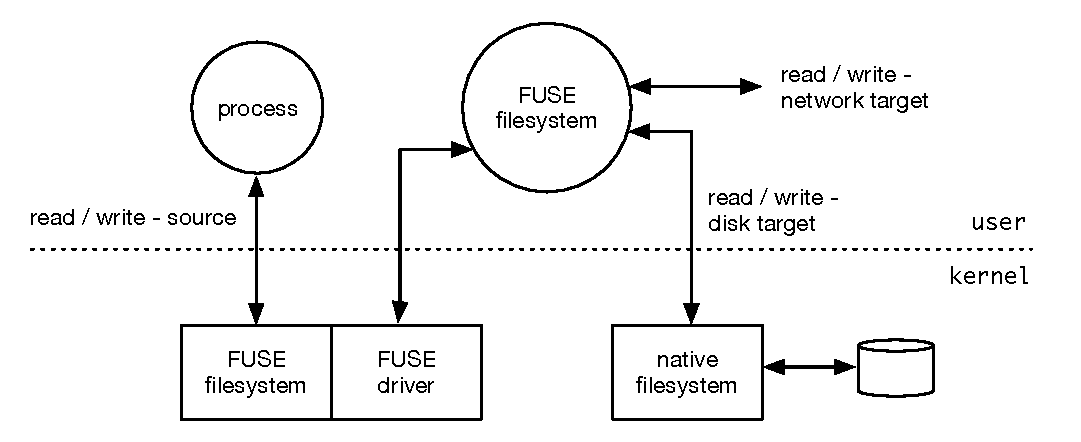
\includegraphics[scale=0.6]{figures/fuse-fs-chap.pdf}
	\centering
	\caption{FUSE filesystems allow development in user-space}
	\label{fig:fuse-fs-chap}
\end{figure}

Applications access files as normal unaware that they are using a FUSE filesystem. Inside the kernel, the FUSE kernel components route file operations up into user-space where they are handled by a FUSE library and the FUSE filesystem component which then routes these calls either back into the kernel to different part of the filesystem or over the network to a remote service. 

cover mount options a little

There are a lot of FUSE-based filesystems. The FUSE Wikipedia page has a large list. We'll describe a few here and then give an example of using one in particular.

\begin{itemize}
	\item s3fs --- the ability to mount an AWS S3 bucket and view the objects as files
	\item EncFS --- a filesystem that encrypts files and contents. Security concerns were raised about
		EncFS and there was rumored to be a newer version which would fix these concerns. That hasn't
		yet happened.
	\item SSHFS --- access to a remote filesystem through use of SSH.
	\item WikipediaFS --- the ability to view Wikipedia pages as if there were local files. It has since
		been deprecated.
\end{itemize}

In section \ref{fuse-chapter} I'll be showing you how to develop two FUSE-based filesystems. The first will just "pass-through" operations whereby part of the file hierarchy will be visible through another directory. Files can be created, deleted and accessed as normal. The second filesystem will add encryption for file names and contents.

%------------------------------------------------------------------------------------------------------------------------------------------------------------------------

\subsection{Demonstrating the SSHFS FUSE Filesystem}\label{ssh-fuse}

I wanted to demonstrate the WikipediaFS filesystem but found that it was deprecated many years ago. The same seems to be somewhat true of SSHFS. The github page indicates that the project is no longer maintained or developed although there have been changes within the last year. The repository has been archived so it's now read-only. It's also available to be installed, at least on Ubuntu. So let's give it a try. First, it needs to be installed:

\begin{lstlisting}
$ [*\bfseries sudo apt install sshfs*]
\end{lstlisting}

\noindent
Next, we'll create a local directory on to which we will mount the remote directory. We run \cf{mount(1)} to verify that it's mounted. Note that the \cf{sshfs} command backgrounds itself.

\begin{lstlisting}
$ [*\bfseries mkdir remote*]
$ [*\bfseries sshfs spate@192.168.4.21:~/src/spfs remote*]
(spate@192.168.4.21) Password:
$ [*\bfseries mount | grep remote*]
spate@192.168.4.21:/Users/spate/src/spfs on /home/spate/remote \
type fuse.sshfs (rw,nosuid,nodev,relatime,user_id=1000,\
group_id=1000)
\end{lstlisting}

\noindent
At this point, all files are visible just as if they were local:

\begin{lstlisting}
$ [*\bfseries ls remote*]
cmds  kern  LICENSE  README  test
$ [*\bfseries ls remote/kern*]
add_stuff  dir.c     Makefile    sp_dir.c   spfs.h  sp_ioctl.c
dir2.c     fillfs.c  sp_alloc.c  sp_file.c  sp_inode.c
\end{lstlisting}

\noindent
You can move around the directory structures, create, remove and read/write files. When you want to unmount the filesystem simply run:

\begin{lstlisting}
$ [*\bfseries fusermount -u remote*]
\end{lstlisting}

\noindent
I spend a lot of time running scripts to sync files between my Mac and my Linux VMs. This looks like a much easier method so happy I gave it a try.

%%%%%%%%%%%%%%%%%%%%%%%%%%%%%%%%%%%%%%%%%%%%%%%%%%%%%%%%%%%%%%%

\section{Physical Filesystems and Partitioning}\label{mkfs-examples}

- grub
- fdisk or whatever is used now
- limitations of disk sizes - relevant any more
- raw vs block devices

\textbf{XXX---example with partitioning and multiple filesystems on same disk / different partitions}

I've partitioned my 1 GB virtual disk into two partitions using \cf{fdisk(8)} so now I have two partitions:

\begin{lstlisting}
# [*\bfseries ls /dev/sd??*]
/dev/sda1  /dev/sda2
\end{lstlisting}

\noindent
And now I can create a filesystem on each partition, mount each filesystem and copy some files into both:

\begin{lstlisting}
# [*\bfseries mkfs -t ext4 /dev/sda1*]
...
# [*\bfseries mkfs -t btrfs /dev/sda2*]
...
# [*\bfseries mount -t ext4 /dev/sda1 /mnt1*]
# [*\bfseries mount -t btrfs /dev/sda2 /mnt2*]
# [*\bfseries cp /etc/* /mnt1 2> /dev/null*]
# [*\bfseries cp /etc/* /mnt2 2> /dev/null*]
# [*\bfseries df -h | grep mnt*]
/dev/sda1        703M  552K  651M   1% /mnt1
/dev/sda2        291M  3.9M  210M   2% /mnt2
# [*\bfseries df -h*]
Filesystem       Size  [*\bfseries Used*] Avail Use% Mounted on
...
/dev/sda1        703M  [*\bfseries 552K*]  651M   1% /mnt1
/dev/sda2        291M  [*\bfseries 3.9M*]  210M   2% /mnt2
\end{lstlisting}

\noindent
Note that although we have copied the same amount of data into each filesystem, the btrfs filesystem has used a lot more space than ext4. Some filesystems use more space for meta-data and some filesystems allocated meta-data up front while others allocate it dynamically therefore usage varies depending on the filesystem type. With the size of today's disks, it's really not a big deal.

%%%%%%%%%%%%%%%%%%%%%%%%%%%%%%%%%%%%%%%%%%%%%%%%%%%%%%%%%%%%

\section{Linux Namespaces}

% https://docs.kernel.org/userspace-api/unshare.html - good doc about unshare(2) and kernel support

Linux \textit{namespaces} are a feature of the Linux kernel that allow for different types of process isolation. Linux partitions different kernel resources such that one group of processes sees one set of resources while another group of processes can see a different set of resources. Namespaces were introduced into the Linux kernel in 2002 with enhancements and extensions continuing over the next several years. Namespaces are a fundamental aspect of how containers are implemented in Linux.

Since Linux kernel version 5.6, there are now eight different kinds of namespaces. All but the MNT namespace are beyond the scope of this book.

\begin{itemize}
	\item \textbf{Mount (MNT)} -- a  list of mount points seen by the processes in this particular namespace. Filesystems can be 
		mounted and unmounted in a mount namespace without impact on the main Linux filesystem.
	\item \textbf{Process ID (PID)} -- this namespace has a different set of PIDs from other namespaces. PID namespaces 
		are nested such that if a process is created it will have a one PID in the current namespace and a different PID
		in all namespaces above it up to the initial PID namespace. The first process created in any new PID namespace 
		is assigned the process ID number 1.
	\item \textbf{Network (NET)} -- 
	\item \textbf{Inter-process Communication IPC)} -- 
	\item \textbf{UTS} -- 
	\item \textbf{User ID (USER)} -- 
	\item \textbf{Control group (CGROUP) Namespace} -- 
	\item \textbf{Time Namespace} -- 
\end{itemize}

\noindent
The MNT namespace is particularly relevant to filesystem access and you will see references to it through various parts of the filesystem code. It will be explained in the next section.

A Linux system starts out with a single namespace of each type and is used by all processes. Processes can create additional namespaces and/or join different namespaces. Namespaces are a fundamental aspect of containers on Linux and will be described in the next section.

Mount namespaces provide isolation regarding the list of mounts as seen by the process/tasks in each namespace. This ensures that different processes/tasks that belong to different mount namespaces will see distinct directories hierarchies.

Namespaces are documented in the \cf{unshare(1)} command and \cf{clone(2)} system call manpages. For an overview see the \cf{mount\_namespaces(7)} manpage.

% https://itnext.io/chroot-cgroups-and-namespaces-an-overview-37124d995e3d - chroot, cgroups and namespaces

More notes:

\begin{enumerate}
	\item Namespaces are often used when untrusted code has to be executed on a given machine without compromising 
		the host OS.
	\item on process namespaces - All ‘ps’-like commands use the virtual procfs file system mount to deliver their functionalities.
	\item Linux processes form a single hierarchy, with all processes rooting at init. Usually privileged processes in this tree can trace or kill other processes.Linux namespace enables us to have many hierarchies of processes with their own “subtrees” such that processes in one subtree cant access or even know of those in another.
	\item If we create a PID namespace and run a process in it, that first process becomes PID 1 in that namespace. 
	\item But this only means that the processes within the new namespace can not see parent process but the parent process namespace can see the child namespace. And the processes within new namespace now have 2 PIDs: one for new namespace and one for global namespace.
	\item Linux kernel now tracks process’s PIDs using upid structure instead of a single pid value. The upid structure tells about the pid and the namespaces where that pid is valid.
	\item There are new APIs - clone(), setns() and unshare() - need to look at them.
The above "flags" (CLONE\_NEWNS, CLONE\_NEWUSER etc) are passed to clone() to create that type of namespace.
\end{enumerate}

%--------------------------------------------------------------------------------------------------------------------------------------------------------------------

\subsection{Shared Subtrees}

Damn! This stuff is complicated!

% https://www.kernel.org/doc/Documentation/filesystems/sharedsubtree.txt - shared subtrees - relevant?
% https://lwn.net/Articles/689856/ - Mount namespaces and shared subtrees

\begin{itemize}
	\item \cf{MS\_SHARED} --  This mount point shares mount and unmount events with other mount points that 
		are members of its “peer group”. When a mount point is added or removed under this mount point, 
		this change will propagate to the peer group, so that the mount or unmount will also take place under 
		each of the peer mount points. Propagation also occurs in the reverse direction, so that mount and 
		unmount events on a peer mount will also propagate to this mount point.
	\item \cf{MS\_PRIVATE} -- This is the converse of a shared mount point. The mount point does not propagate 
		events to any peers, and does not receive propagation events from any peers.
	\item \cf{MS\_SLAVE} -- This propagation type sits midway between shared and private. A slave mount has a 
		master — a shared peer group whose members propagate mount and unmount events to the slave mount. 
		However, the slave mount does not propagate events to the master peer group.
	\item \cf{MS\_UNBINDABLE} -- Does not receive or forward any propagation events and cannot be bind mounted.
\end{itemize}

\noindent
xxx
	
%--------------------------------------------------------------------------------------------------------------------------------------------------------------------

\subsection{Root and \cf{chroot} Environments}

%<<<
In a Unix-like OS, root directory(/) is the top directory. root file system sits on the same disk partition where root directory is located. And it is on top of this root file system that all other file systems are mounted. All file system entries branch out of this root. This is the system’s actual root.

But each process has its own idea of what the root directory is. By default, it is actual system root but we can change this by using chroot() system call. We can have a different root so that we can create a separate environment to run so that it becomes easier to run and debug the process. Or it may also be to use legacy dependencies and libraries for the process.

It may appear that by separating a process using chroot()we ensure security by restricting the process not to access outside its environment. But in reality that is not very true. chroot() simply modifies pathname lookups for a process and its children , prepending the new root path to any name starting with /.Current directory is not modified and relative paths can refer any locations outside of new root.
%>>>

Yeah so can you chroot when logging in to solve this???

\subsection{Linux cgroups to Isolate and Manage Resources}

%<<<
Control groups(cgroups) is a Linux kernel feature which limits, isolates and measures resource usage of a group of processes. Resources quotas for memory, CPU, network and IO can be set. These were made part of Linux kernel in Linux 2.6.24.
%>>>

sound great for virtualization - yes. what we want is:

%<<<
Suppose we have an application we want to isolate usage for. Lets call it A1. Lets call rest of system as S. We will create a control group and assign resource limits on it: say 3GB of memory limit and 70\% of CPU. Then we can add requisite application’s process id to the group and application resource usage now is throttled. Though the application may exceed the limits in normal scenarios, it will be throttled back to pre set limits in case system is facing resource crunch. This makes even more sense when we are handling many VMs running on a machine-have a cgroup for VMs and throttle them individually to a set limit when resource contention happens.
%>>>

to install:

sudo apt-get install cgroup-bin cgroup-lite cgroup-tools cgroupfs-mount libcgroup1

%<<<
We can see a /cgroup directory created: this is used as mount point for cgroup virtual filesystems. etc/cgconfig.conf file gives info on what all mounts to expect. All controllers are mounted to /cgroup followed by controller name. eg/- /cgroup/memory.To mount the requisite controllers, run sudo service cgconfig restart .Following this we see directories in /cgroup, each of which can be used to manage a cgroup subsystem.
%>>>

https://itnext.io/chroot-cgroups-and-namespaces-an-overview-37124d995e3d - gives an example of using cgroups with a process that allocates more memory than allowed and gets killed. OK, good so far.

%--------------------------------------------------------------------------------------------------------------------------------------------------------------------

\subsection{Mount Namespace Example}

It always helps to see things in practice. This example shows how to create mount namespaces and show how mounts are shared or not shared depending on how \textbf{XXX - TBD}

\begin{lstlisting}
$ [*\bfseries sudo unshare -m bash*]
# [*\bfseries mount -t tmpfs tmpfs /mnt*]
# [*\bfseries touch /mnt/file*]
\end{lstlisting}

\noindent
in another terminal:

\begin{lstlisting}
$ [*\bfseries ls /mnt*]
lost+found/
\end{lstlisting}

\noindent
the newly created file is not visible. Further, once you exit the namespace, the file and mount point are no longer visible.

But this doesn't work for disk-based mount points. even if you create two namespaces and then mount -t spfs in one namespace, it's visible everywhere. XXX - Must be doing something wrong or just not understanding this properly.

Inside \cf{proc} you can see the mounting points visible for a specific process through the following paths:

\begin{enumerate}
	\item \cf{/proc/[PID]/mounts}
	\item \cf{/proc/[PID]/mountinfo}
	\item \cf{/proc/[PID]/mountstats}
\end{enumerate}

%--------------------------------------------------------------------------------------------------------------------------------------------------------------------

\subsection{Containers}

% https://www.baeldung.com/ops/docker-container-filesystem
% https://medium.com/@BeNitinAgarwal/docker-containers-filesystem-demystified-b6ed8112a04a - Docker Container’s Filesystem Demystified

Don't do too much. Just as things related to filesystems.

The \cf{fakeroot(1} command allows another command to be run such that it appears that the UID of the command has root privileges. A quick example:

\begin{lstlisting}
$ [*\bfseries fakeroot bash*]
$ [*\bfseries id*]
uid=0(root) gid=0(root) groups=0(root),4(adm),24(cdrom),
27(sudo),30(dip),46(plugdev),108(lxd),1000(spate)
\end{lstlisting}

\noindent
The original goal of \cf{fakeroot} was to allow for creation of packages while running as a normal user. This allowed the user to create files with permissions and ownership that would normally require root access to achieve, thus \textit{fake root} privileges. This is particularly useful for creating Linux distribution packages, where the package maintainer does not need to run the process as root.

%--------------------------------------------------------------------------------------------------------------------------------------------------------------------

\subsection{Creating a Container by Hand}

To show how containers interact with the Linux filesystem, this example builds a container by hand XXX

Building a container by hand using namespaces: The mount namespace % https://www.redhat.com/sysadmin/mount-namespaces

\begin{lstlisting}
$ unshare -m - ??? - need sudo -no?
\end{lstlisting}

-> unshare - run program in new namespaces

try it and cd to \$HOME - very odd

uses "Alpine Linux tarball" - small secure Linux something or other

talks about fakeroot command - good article here - https://unix.stackexchange.com/questions/9714/what-is-the-need-for-fakeroot-command-in-linux

\begin{lstlisting}
$ sudo apt install fakeroot
\end{lstlisting}

run it and you get a root prompt

\begin{lstlisting}
22.04-crash$ fakeroot
22.04-crash$ id
uid=0(root) gid=0(root) groups=0(root),4(adm),24(cdrom),27(sudo),30(dip),46(plugdev),110(lxd),1000(spate)

22.04-crash$ pwd
/home/spate/spfs/debug
\end{lstlisting}

in the same directory where you run the command XXX not sure how this fits in????

XXX - look at  mount\_namespaces(7)

%%%%%%%%%%%%%%%%%%%%%%%%%%%%%%%%%%%%%%%%%%%%%%%%%%%%%%%%%%%%

\section{Filesystem Operations}

There are several commands that related to filesystems such as mounting and unmounting filesystems, remounting or collection data about filesystem statistics such as running the \cf{df(1)} command. This section covers relevant commands in this area.

%------------------------------------------------------------------------------------------------------------------------------------------------------------------------

\subsection{Making a Filesystem}

Filesystems can be created using the \cf{mkfs(1)} command which is really just a front-end for a filesystem-specific \cf{mkfs} command such as \cf{mkfs.ext4(8)} and \cf{mkfs.xfs(8)}.

The source code for many filesystem commands can be found at https://github.com/util-linux/util-linux. A comment in \cf{mkfs.c} file as well as the manpage for \cf{mkfs(8)} specifies that the command is deprecated in favor of the individual commands. 

For the main Linux filesystems, Table \ref{table:mkfs} shows its \cf{mkfs} command together with the package that contains the source code. 

\begin{table}
\begin{center}
\begin{tabular}{|c|l|l|l|}
\hline
\rowcolor{gray!30}
\textbf{FS} & \textbf{mkfs command} & \textbf{Utilities} & \textbf{Source Code} \\
\hline
ext3 & \cf{mkfs.ext3(8)} & e2fsprogs  & https://github.com/tytso/e2fsprogs    \\ 
\hline
ext4 & \cf{mkfs.ext4(8)} & e2fsprogs  & https://github.com/tytso/e2fsprogs     \\
\hline
btrfs & \cf{mkfs.btrfs(8)} & btrfs-progs  & https://github.com/kdave/btrfs-progs \\
\hline
XFS & \cf{mkfs.xfs(8)}  &  xfsprogs & https://github.com/mtanski/xfsprogs \\
\hline
\end{tabular}
\end{center}
\caption{Various mkfs commands for the major filesystems}
\label{table:mkfs}
\end{table}

\noindent
You can still use \cf{mkfs(8)} for now. If no options are specified, en ext2 filesystem is created. To specify a filesystem type use the \cf{-t} option (see section \ref{mkfs-examples} for examples. Take a look at the source code. It's a very simple front-end to the specific filesystem commands which can be found in \cf{/sbin}:

\begin{lstlisting}
$ [*\bfseries ls /sbin/mkfs**]
/sbin/mkfs        /sbin/mkfs.cramfs /sbin/mkfs.ext4  
/sbin/mkfs.msdos  /sbin/mkfs.bfs    /sbin/mkfs.ext2   
/sbin/mkfs.fat    /sbin/mkfs.vfat   /sbin/mkfs.btrfs s
/sbin/mkfs.ext3   /sbin/mkfs.minix  /sbin/mkfs.xfs
\end{lstlisting}

%------------------------------------------------------------------------------------------------------------------------------------------------------------------------

\subsection{Mounting Filesystems}\label{fsmounting}

\textbf{XXX---there is a section in the prog chapter. Need to cover mntopts etc here}

The following is from Documentation/filesystems/sharedsubtree.rst - need to tie in with namespaces
\begin{quote}
    Note: mount(8) command now supports the --make-shared flag,
    so the sample 'smount' program is no longer needed and has been
    removed.
\end{quote}

\subsection{The Mount Table}

The source code for the \cf{mount(8)} command can also be found at https://github.com/util-linux/util-linux. It has quite a lot of work to do as you can see from the manpage, mostly in terms of managing a lot of possible options including passing filesystem-specific options to the kernel when it invokes the \cf{mount(2)} system call.

The most basic forms of calling \cf{mount(8)} are as follows:

\begin{lstlisting}
# [*\bfseries mount -t ext4 /dev/sda1 /mnt*]
# [*\bfseries mount /dev/sda1 /mnt*]
# [*\bfseries mount /mnt*]
\end{lstlisting}

\noindent
If the \cf{-t} option is passed, \cf{mount} will find and invoke the filesystem-specific \cf{mount} command. In the second two cases, it needs to determine what the additional parameters are and it does this but looking in the \cf{/etc/fstab} file (\cf{fstab(5)}). This file lists the filesystems to be mounted both during the bootstrap process and at a later time. The order of entries in this file is critical. There are six fields in each line of \cf{fstab} which are listed in the order in which they should appear. Each field name shown is the field within \cf{struct mntent}, the structure returned by a call to \cf{getmntent(3)}. We borrow some words from the manpage but for details, please refer to the manpage.

\begin{enumerate}
	\item \cf{fs\_spec} --- this field describes the block special device, remote filesystem or 
		filesystem image for loop device to be mounted or swap file or swap
		partition to be enabled.
	\item \cf{fs\_file} --- this field describes the mount point (target) for the filesystem. For
		swap partitions, this field should be specified as \cf{none}.
	\item \cf{fs\_vfstype} --- the type of the filesystem (for example "ext4", "xfs" and so on). If \cf{swap}
		is specified, this is a file or partition to be used as a swap device. We cover swapping in 
		section \ref{swap}.
	\item \cf{fs\_mntops} --- a comma-separated list of mount options which must include \cf{ro} or \cf{rw}
		(read-only or read/write).
	\item \cf{fs\_freq} --- this field is used by \cf{dump(8)} command which will be covered in section \ref{backups}
	\item \cf{fs\_passno} --- this field is used by \cf{fsck(8)} to determine the order in which filesystem 
		checks are done at boot time. The root filesystem should be specified with a \cf{fs\_passno} of \cf{1}. 
		Other filesystems should have a \cf{fs\_passno} of 2
\end{enumerate}

\noindent
For device names you can use the actual path to the partition (for example \cf{/dev/sda1}). By preference,  \cf{LABEL} or \cf{UUID} should be used as device names can change as disks are added or removed. Here is an example of the largely unreadable \cf{fstab} on my simple Ubuntu VM. I've abbreviated the long device names. Note that lines starting with "\#" are comments and are ignored.

\begin{lstlisting}
# <file system> <mount point> <type>  <options> <dump>  <pass>
# / was on /dev/ubuntu-vg/ubuntu-lv during curtin installation
/dev/disk/by-id/dm-uuid-LVM-AI...62ciB / ext4 defaults 0 1
# /boot was on /dev/vda2 during curtin installation
/dev/disk/by-uuid/03fb45b9...8427 /boot ext4 defaults 0 1
# /boot/efi was on /dev/vda1 during curtin installation
/dev/disk/by-uuid/368C-2362 /boot/efi vfat defaults 0 1
/swap.img       none    swap    sw      0       0
\end{lstlisting}

\noindent
You can see things a little more clearly by running the following:

\begin{lstlisting}
# [*\bfseries df -h*]
Filesystem               Size  Used Avail Use% Mounted on
tmpfs                    392M  1.4M  390M   1% /run
/dev/mapper/ubuntu--lv   38G   11G   25G  31% /
tmpfs                    2.0G     0  2.0G   0% /dev/shm
tmpfs                    5.0M     0  5.0M   0% /run/lock
/dev/vda2                2.0G  494M  1.4G  28% /boot
/dev/vda1                1.1G  5.1M  1.1G   1% /boot/efi
tmpfs                    392M  4.0K  392M   1% /run/user/1000
# [*\bfseries swapon*]
NAME      TYPE SIZE USED PRIO
/swap.img file 3.8G   3M   -2
\end{lstlisting}

\noindent
There are two ways to view the current list of mounted filesystem. Either by looking at \cf{/etc/mtab} or through \cf{/proc/mounts}. If you search for "linux mtab /proc/mounts" you will see that there has been differences between the two with \cf{/proc/mounts} being more up to date. The \cf{/etc/mtab} file has generally been kept up to date by scripts which take the information from \cf{/proc/mounts} for applications that still use \cf{/etc/mtab}. That information may refer to some or older versions of Linux. On my Ubuntu VM I have:

\begin{lstlisting}
# [*\bfseries diff /etc/mtab /proc/mounts*]
\end{lstlisting}

\noindent
which shows that both have the same information. Digging under the covers:

\begin{lstlisting}
# [*\bfseries ls -l /etc/mtab*]
lrwxrwxrwx 1 root root 19 Oct 19 14:05 /etc/mtab \
    -> ../proc/self/mounts
# [*\bfseries diff /proc/mounts /proc/self/mounts*]
\end{lstlisting}

\noindent
Therefore the \cf{/proc} is the correct one. My next thought was to see what the \cf{df(1)} command used so I ran the following:

\begin{lstlisting}
# [*\bfseries strace -f -o s.out df -h*]
\end{lstlisting}

\noindent 
and searched through \cf{s.out}. This is what I found:

\begin{lstlisting}
168999 openat(AT_FDCWD, "/proc/self/mountinfo", O_RDONLY) = 3
\end{lstlisting}

\noindent
Great! So not only do we have \cf{/proc/mounts} and \cf{/proc/self/mounts} but we also have \cf{/proc/self/mountinfo}. Furthermore:

\begin{lstlisting}
$ [*\bfseries ls -l /proc/mounts*]
lrwxrwxrwx 1 root root 11 Nov 28 18:01 /proc/mounts \
    -> self/mounts
\end{lstlisting}

%{\bfseries XXX---Need to read this etc - https://serverfault.com/questions/581178/proc-self-mountinfo-per-mount-options-vs-per-super-options}

%------------------------------------------------------------------------------------------------------------------------------------------------------------------

\subsection{Automounting Filesystems}

\textbf{It's covered during pathname resolution so far when crossing mount points}

%------------------------------------------------------------------------------------------------------------------------------------------------------------------

\subsection{Unmounting Filesystems}

The \cf{umount(1)} command underpinned by the \cf{umount(2)} system call is used to unmount a filesystem. Either the mount point or the device can be used as an argument. Unmounting a filesystem is easy, as long as it works. It can be as simple as the following example shows:

\begin{lstlisting}
$ [*\bfseries sudo mount -t spfs /dev/sda1 /mnt*]
$ [*\bfseries sudo umount /mnt*]
$
\end{lstlisting}

\noindent
A filesystem that resides on \cf{/dev/sda1} is mounted on \cf{/mnt} and then immediately unmounted. You won't see anything printed but the \cf{umount(1)} command unless there is an issue.

Filesystems can be force unmounted which is particularly useful for network filesystem mounts. XXX

%------------------------------------------------------------------------------------------------------------------------------------------------------------------

\subsection{The \cf{lsof(1)} Command}

If a filesystem is busy, you will need to locate the users and/or processes that are using the filesystem. This is where the \cf{lsof(1)} command comes in useful. Assume that a filesystem in mounted on \cf{/mnt} and in one terminal, the following command is run:

\begin{lstlisting}
$ [*\bfseries less /mnt/lorem-ipsum*]
Lorem ipsum dolor sit amet, consectetur
...
\end{lstlisting}

\noindent
an attempt is made to unmount it:

\begin{lstlisting}
$ [*\bfseries sudo umount /mnt*]
umount: /mnt: target is busy.
\end{lstlisting}

\noindent
The \cf{lsof(1)} command can be used to list what processes are access files in this filesystem. In this simple example, here is the output shown when running \cf{lsof} on the mountpoint:

\begin{lstlisting}
$ [*\bfseries lsof /mnt*]
COMMAND  PID  USER FD TYPE DEVICE SIZE/OFF NODE NAME
less    1012 spate 4r  REG    7,7   2972    8   /mnt/lorem-ipsum
\end{lstlisting}

\noindent
This allows an administrator to locate the user and tell them to exit the filesystem or the process can be killed.

% https://stackoverflow.com/questions/7878707/how-to-unmount-a-busy-device

%%%%%%%%%%%%%%%%%%%%%%%%%%%%%%%%%%%%%%%%%%%%%%%%%%%%%%%%%%%%

\subsection{Reporting File System Disk Space Usage}

In the previous section we displayed the result of running \cf{df -h} and mentioned that it gets its information from opening and reading \cf{/proc/self/mountinfo}. So what is in this file? Let's take a look at the first few lines:

\begin{lstlisting}
26 32 0:24 / /sys rw,...,relatime shared:7 - sysfs sysfs rw
27 32 0:25 / /proc rw,...,relatime shared:13 - proc proc rw
28 32 0:5 / /dev rw,...,relatime shared:2 - devtmpfs udev ...
29 28 0:26 / /dev/pts rw,...,relatime shared:3 - devpts rw ...
\end{lstlisting}

\noindent
{\bfseries XXX---no idea! come back and explain this}
I've removed some arguments so the output will fit on the screen so you should try running this and see the full set of arguments.

\subsection{Fixing Filesystems with \cf{fsck}}

When a filesystem is mounted, one of the first things that the filesystem does it to mark the filesystem as dirty. If the system crashes, the filesystem will need to be repaired. This is where the \cf{fsck(8)}, the FileSystem CHecker, command comes into play. There is a generic \cf{fsck(8)} command as well as individual filesystem \cf{fsck} commands.

Here is partial output from running \cf{fsck} on a UFS filesystem. This demonstrates the types of messages that used to be display. In this example, \cf{fsck} is running in interactive mode. I always found it amusing that system administrators would know how to answer these questions. As time evolved, \cf{fsck} was generally run in non-interactive mode and the utility was left to decide how to fix things.

\begin{lstlisting}
# [*\bfseries fsck -t ufs -fy /dev/vtbd0p2*]
** /dev/vtbd0p2 (NO WRITE)
SETTING DIRTY FLAG IN READ_ONLY MODE

UNEXPECTED SOFT UPDATE INCONSISTENCY
** Last Mounted on /
** Root file system
** Phase 1 - Check Blocks and Sizes
** Phase 2 - Check Pathnames
** Phase 3 - Check Connectivity
** Phase 4 - Check Reference Counts
** Phase 5 - Check Cyl groups
FREE BLK COUNT(S) WRONG IN SUPERBLK
SALVAGE? no
...
\end{lstlisting}

\noindent
\textbf{talk about lost+found}

\textbf{XXX---how much time to spend on this?}

\subsection{Filesystem Debugging}

In addition to running \cf{fsck(8)} on a filesystem to repair it, most filesystems have another tool that allows administrators or developers to debug the filesystem. This allows reading and modifying various structures. Such a tool is invaluable when developing a filesystem in addition to log messages to see when objects get written to disk and to make sure that all counts and links are updated correctly. Usually such a tool is run when the filesystem is unmounted but for filesystem development, running when the filesystem is mounted is very useful. 

Each filesystem debugger is different but there will be some similarities in terms of displaying directories, inodes and perhaps being able to walk through the filesystem (similar to using the \cf{cd} command.

Before we run \cf{debugfs(8)} let's take a quick look at the contents of the filesystem that we're going to debug. We have 2 files and one directory in addition to the root directory:

\begin{lstlisting}
/mnt1
/mnt1/lorem-ipsum
/mnt1/mydir
/mnt1/mydir/hello.txt
\end{lstlisting}

\noindent
To enter the debugger, simply run the command against the device where the filesystem resides. Type \cf{?} to list the available commands.

\begin{lstlisting}
# [*\bfseries debugfs /dev/sda1*]
debugfs 1.46.5 (30-Dec-2021)
debugfs:  [*\bfseries ?*]
Available debugfs requests:

show_debugfs_params, params Show debugfs parameters
open_filesys, open       Open a filesystem
close_filesys, close     Close the filesystem
freefrag, e2freefrag     Report free space fragmentation
feature, features        Set/print superblock features
....
\end{lstlisting}

\noindent
Next we show how to navigate through the directory structure, stat files and display their contents:

\begin{lstlisting}
debugfs:  [*\bfseries pwd*]
[pwd]   INODE:      2  PATH: /
[root]  INODE:      2  PATH: /
debugfs:  [*\bfseries ls*]
2 (12)     2 (12)  ..    11 (20) lorem-ipsum   12 (4040) mydir
debugfs:  [*\bfseries cd mydir*]
debugfs:  [*\bfseries ls*]
12  (12) .    2  (12) ..    13  (4060) hello.txt
debugfs:  [*\bfseries stat hello.txt*]
Inode: 13   Type: regular    Mode:  0644   Flags: 0x80000
Generation: 885043848    Version: 0x00000000:00000001
User:     0   Group:     0   Project:     0   Size: 6
File ACL: 0
Links: 1   Blockcount: 8
Fragment:  Address: 0    Number: 0    Size: 0
ctime: 0x6390b30e:dd5258b0 -- Wed Dec  7 15:36:46 2022
atime: 0x6390b30e:dd5258b0 -- Wed Dec  7 15:36:46 2022
mtime: 0x6390b30e:dd5258b0 -- Wed Dec  7 15:36:46 2022
crtime: 0x6390b30e:dd5258b0 -- Wed Dec  7 15:36:46 2022
Size of extra inode fields: 32
Inode checksum: 0x7cc9f75a
EXTENTS:
(0):33792
debugfs:  [*\bfseries bd 33792*]
0000  6865 6c6c 6f0a 0000 0000 0000 0000 0000  hello...........
0020  0000 0000 0000 0000 0000 0000 0000 0000  ................
*
\end{lstlisting}

\noindent 
There are many options for navigating through the filesystem, displaying inodes, blocks, xattrs and other objects. The real use comes in being able to modify various structures including inodes and the superblock, replaying the journal and so on. A word of warning---if you're planning on modifying data structures on disk, be very careful. I would recommend creating a small demo filesystem that allows to mirror the operations you plan on performing on the real filesystem. You should also run the filesystem's \cf{fsck} command after you make any modifications to make sure that the filesystem is structurally intact.

A full list of commands can be found in the \cf{debugfs(8)} manpage.

%%%%%%%%%%%%%%%%%%%%%%%%%%%%%%%%%%%%%%%%%%%%%%%%%%%%%%%%%%%%

\section{Loopback Mounts}

Right place? 

Even if you are not familiar with loop devices, you will likely have seen them at some point while using Linux. Furthermore, if you use Ubuntu, you’ll see several loop devices by running te \cf{lsblk} command:

\begin{lstlisting}
$ [*\bfseries lsblk*]
NAME    MAJ:MIN RM   SIZE RO TYPE MOUNTPOINTS
loop0     7:0    0    59M  1 loop /snap/core20/1740
loop1     7:1    0  59.1M  1 loop /snap/core20/1782
loop2     7:2    0 132.8M  1 loop /snap/lxd/24242
loop3     7:3    0 139.3M  1 loop /snap/lxd/24331
loop4     7:4    0  43.2M  1 loop /snap/snapd/17954
loop5     7:5    0    43M  1 loop /snap/snapd/17885
...
\end{lstlisting}

\noindent
This is due to \textit{snaps} which is a software packaging and deployment system developed by Canonical. Snap applications are mounted as loop devices.

In a virtualized world, it's easy to create new devices to play with when adding new filesystems, experimenting with volume managers and so on. But there is also another way which is also very useful, not just for experimentation but for \textbf{containers - check}. This is where \textit{loopback devices} come into play. You can also create very small devices / filesystems if you're limited on space.

Great for playing with filesystems xxx

\textbf{XXX---come back here once namespaces, virtualization etc are well understood}

XXX odd because you can run mkfs -t on a regular file so we don't need loopback devices. So when are they really useful? See here for info - % https://www.tecmint.com/create-virtual-harddisk-volume-in-linux/

Figure \ref{fig:loopback} shows how filesystems are accessed through a loop device. There is a file called \cf{mydevice.img} in the root filesystem and onto which a loop device has been attached. The \cf{/dev/loop2} block device can then be used to create an ext4 filesystem which is then mounted at \cf{/mnt}.

\begin{figure}
	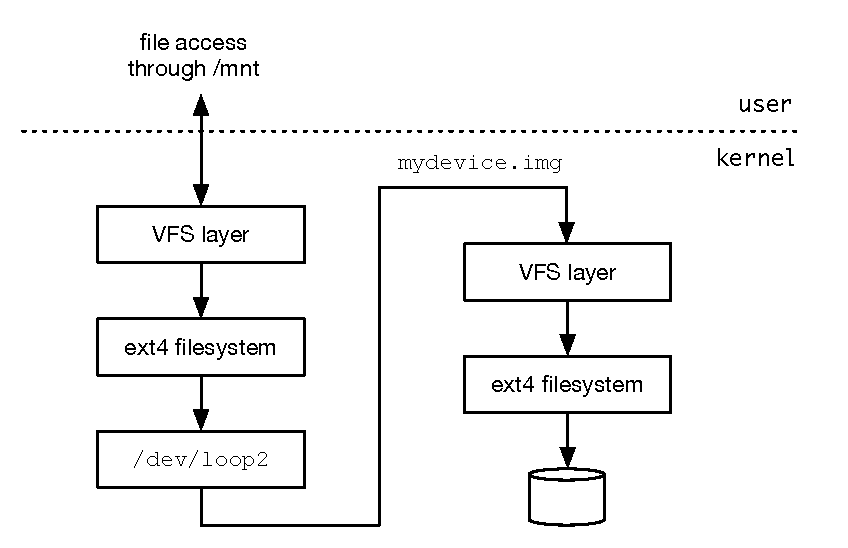
\includegraphics[scale=0.6]{figures/loopback.pdf}
	\centering
	\caption{Accessing a filesystem through a loop device}
	\label{fig:loopback}
\end{figure}

\noindent
xxx

\subsection{Demonstrating Loopback Devices}

This example shows how to create the loop device shown in figure \ref{fig:loopback}, create an ext4 filesystem on it, mount it to make it available for general use.

There are only a few simple steps needed to create a loopback device, add a filesystem and mount it to make it available. First of all, we created a 10 MB file:

\begin{lstlisting}
$ [*\bfseries dd if=/dev/zero of=~/mydevice.img bs=1024k count=10*]
5+0 records in
5+0 records out
5242880 bytes (5.2 MB, 5.0 MiB) copied, 0.00927079 s, 566 MB/s
\end{lstlisting}

\noindent
You can experiment with sizes. If you make it 5 MB, it will be too small for ext4 to add a journal but 10 MB is fine. The next step is to call \cf{losetup} to create a loopback device. The \cf{find} option locates the first available loop device and the \cf{show} option displays which loop device was assigned.

\begin{lstlisting}
$ [*\bfseries sudo losetup --find --show mydevice.img *]
/dev/loop2
\end{lstlisting}

\noindent
The device is accessible via \cf{/dev/loop2} so the next step is to make a filesystem on it, mount it and show space available:

\begin{lstlisting}
$ [*\bfseries sudo mkfs -t ext4 /dev/loop2*]
mke2fs 1.46.5 (30-Dec-2021)
Discarding device blocks: done                            
Creating filesystem with 2560 4k blocks and 2560 inodes

Allocating group tables: done                            
Writing inode tables: done                            
Creating journal (1024 blocks): done
Writing superblocks and filesystem accounting information: done
$ [*\bfseries sudo mount /dev/loop2 /mnt*]
mount: /mnt: /dev/loop2 already mounted on /mnt.
$ [*\bfseries df -h /mnt*]
Filesystem      Size  Used Avail Use% Mounted on
/dev/loop2      5.4M   24K  4.7M   1% /mnt
\end{lstlisting}

\noindent
It looks like, and will function like, any other filesystem. Once you no longer need the filesystem/device you can unmount it and call \cf{losetup} to detach the device. You can keep the file or remove it as needed.

\begin{lstlisting}
$ [*\bfseries sudo umount /mnt*]
$ [*\bfseries sudo losetup --detach /dev/loop2*]
\end{lstlisting}

\noindent
Once mounted, it looks like, and will function like, any other ext4 filesystem but with an additional overhead since there is now an ext4 filesystem on top of an ext4 file residing in another ext4 filesystem. 

Once you no longer need the filesystem/device you can unmount it and call \cf{losetup} to detach the device. You can keep the file or remove it as needed.

%%%%%%%%%%%%%%%%%%%%%%%%%%%%%%%%%%%%%%%%%%%%%%%%%%%%%%%%%%%%

\section{Client Caching With FS-Cache}

\textbf{is this the right place to cover this? I don't think so but come back later. Perhaps "miscelaneous topics"}

% https://www.kernel.org/doc/html/latest/filesystems/caching/fscache.html

FS-Cache is a persistent local cache introduced into Linux by Red Hat in 2001. It allows file systems to take data that has been retrieved from over the network and cache it on local disk. The goal is to help minimize network traffic for users on a client accessing data from a file system mounted over the network. NFS is one such example and an NFS mount option instructs the client to mount the NFS share with FS-Cache enabled.

Why not just utilize the page cache? What are the tradoffs? Data out of sync? Multiple users accessing the same files?


\begin{table}[h]
\begin{tabular}{ll}
\parbox[l]{0.6in}{
\includegraphics[scale=0.8]{figures/src-xref.pdf}} & \parbox[l]{4in}{\small{The FS-cache code can be found in \cf{fs/fscache}. There are only 2700 LOC.}}
\end{tabular}
\end{table}

\noindent
Figure \ref{fig:fscache} shows how FS-Cache works. \textbf{XXX---not sure this is correct. Come back once i figure it out}

\begin{figure}[h]
	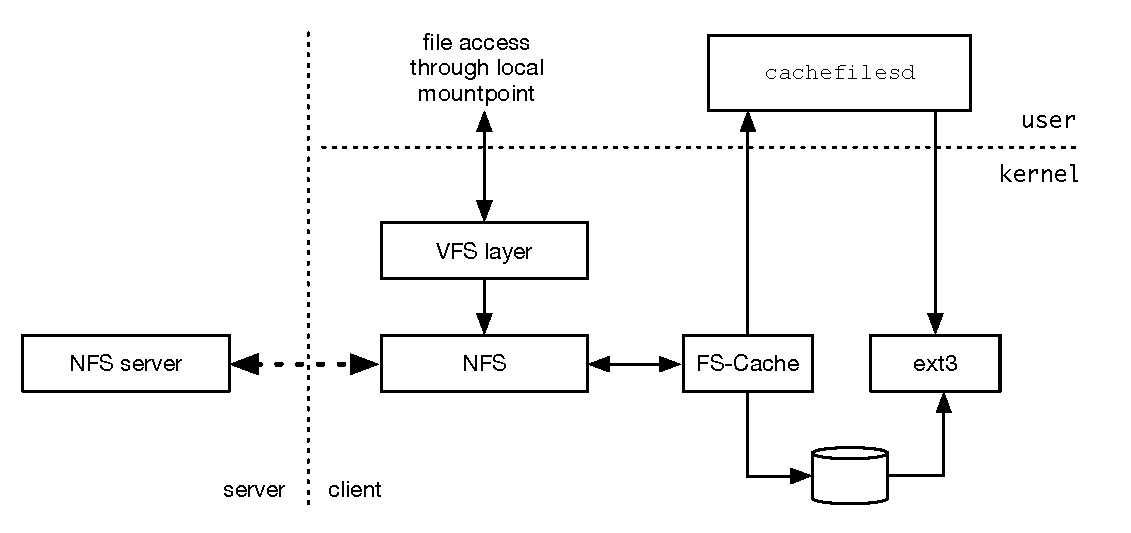
\includegraphics[scale=0.6]{figures/fscache.pdf}
	\centering
	\caption{Client caching with FS-Cache}
	\label{fig:fscache}
\end{figure}

\noindent
The goal of FS-Cache is that it should be as transparent as possible to the users and administrators of a system. In what circumstances is this transparency not achieved? \textbf{XXX---need to find out}.

FS-Cache does not alter the basic operation of a file system that works over the network - it merely provides that file system with a persistent place in which it can cache data. For instance, a client can still mount an NFS share whether or not FS-Cache is enabled. In addition, cached NFS can handle files that won't fit into the cache (whether individually or collectively) as files can be partially cached and do not have to be read completely up front. FS-Cache also hides all I/O errors that occur in the cache from the client file system driver.

Blah blah - NFS will not use FS-Cache unless explicitly stated when mounted as follows:

\begin{lstlisting}
# [*\bfseries mount nfs-share:/ /mount/point -o fsc}
\end{lstlisting}

\noindent
XXX - change args - try it first

%%%%%%%%%%%%%%%%%%%%%%%%%%%%%%%%%%%%%%%%%%%%%%%%%%%%%%%%%%%%

\section{Network Filesystems}

% https://developer.ibm.com/tutorials/l-network-filesystems/ - nice article

Simply put, a network file system allows a remote client to access a filesystem over a network in a similar way to a local file system. Developed over the course of forty years, Sun's NFS (Network Filesystem) has become the dominant network filesystem and has been ported to and ran on just about every operating system developed over that period of time. But NFS isn't the only network filesystem that Linux supports. NFS will be described soon but here are some other network filesystems that Linux supports:

% https://maxammann.org/posts/2022/01/linux-file-system-comparison/ - other nw fs

\begin{itemize}
	\item dav -- GVFS?
	\item davfs2 -- GVFS?
	\item sftp -- GVFS?
	\item SMB -- 
	\item CIFS -- 
	\item SSHFS -- a FUSE-based filesystem that runs on top of the SSH protocol, is accessible by non-root users and makes
		a remote directory visible through a local directory. 
\end{itemize}

\noindent
Which filesystem to use can depend on several factors - TBD - % https://serverfault.com/questions/196285/secure-network-filesystems-for-linux-what-are-people-doing

Section \ref{ssh-fs} shows an example of running SSHFS.

\subsection{NFS -- the Network File System}

NFS has been the most popular network filesystem for several decades now. It started at Sun Microsystems in 1984. The initial release (version 1) was primarily used in-house. This was followed by three major versions which will be described below.

The original paper \textit{The Sun Network Filesystem: Design, Implementation and Experience} can be found with the following link. It describes the goals of the project, how NFS utilized the new VFS/vnode architecture, architecture, design and implementation. The \textit{hard issues} are also described such as file locking.

\begin{table}[h]
\begin{tabular}{lcl}
\parbox[r]{0.5in}{
\includegraphics[scale=0.15]{figures/url.png}} & \parbox[l]{0.55in}{URL \arabic{urls} -- } & \parbox[l]{3in}{\cf{https://tinyurl.com/5f5tyakz}}
\end{tabular}
\end{table}
\stepcounter{urls}
% https://www.cs.ucf.edu/~eurip/papers/sandbergnfs.pdf

\noindent
Figure \ref{fig:nfs} shows the overall architecture of NFS as it was in the 1980s and also, as it is now in the Linux kernel today. There are actually two distinct filesystems, one on the client and one on the server. The client component appears as any other filesystem but takes VFS-level requests and communicates with the NFS server to fulfill them using NFS messages defined in the RFC standard. NFS was originally built on-top of UDP but for many years has primarily run over TCP/IP.

\begin{figure}[h]
	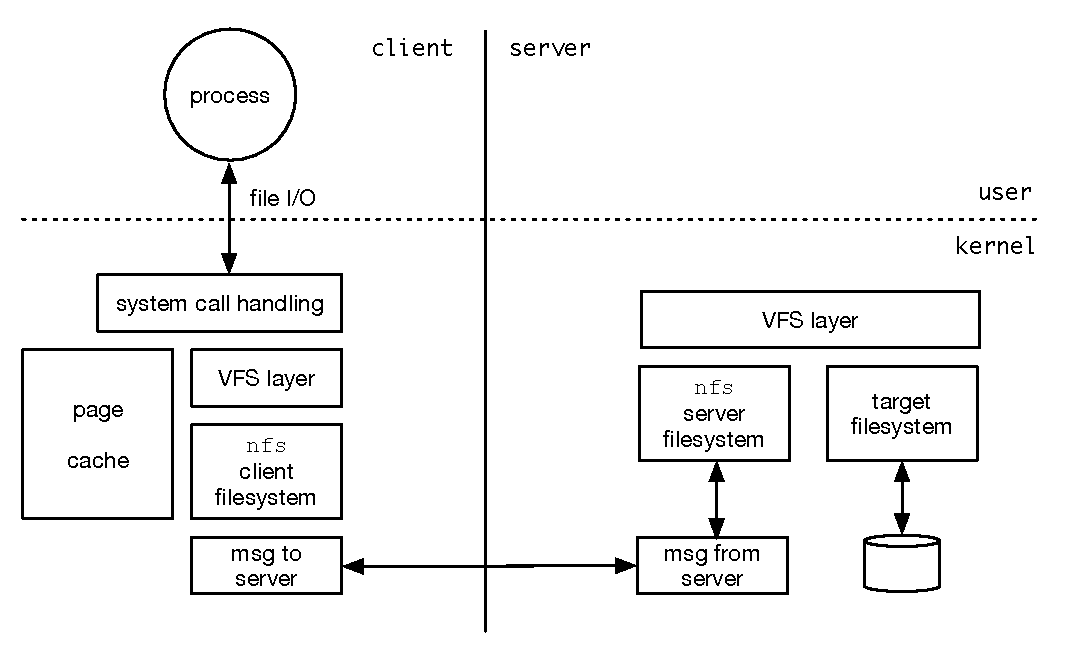
\includegraphics[scale=0.6]{figures/nfs.pdf}
	\centering
	\caption{NFS client and server}
	\label{fig:nfs}
\end{figure}

\noindent
NFS version 2 was defined in RFC 1094 and released in 1989, NFS v2 worked on top of UDP (User  Datagram Protocol) with the goal of being stateless. This meant that the NFS server was unaware of the clients accessing it therefore locking was implemented outside of the protocol. NFS v2 had a 2 GB file limit and poor performance due to synchronous writes. It would take  another few years before the Large File Summit (LFS) came into being with the goals of accessing files greater  than 2 GB. And 32-bit architectures were prevalent. NFS v2 was implemented on the new VFS/vnode architecture.

NFS version 3, defined in RFC 1813 and released in June 1995 had two main goals: add support for \textit{large files} (> 2 GB - 1) and improve performance. In addition to 64-bit file offsets, there were performance improvements in the following areas:

\begin{itemize}
	\item handling asynchronous writes on the server, to improve write performance.
	\item additional file attributes returned for many operations removing the need to keep making additional calls to retrieve them.
	\item a new \cf{READDIRPLUS} operation for which the server returned file handles and attributes along with file 
		names when scanning a directory.
\end{itemize}

\noindent
NFS was becoming very popular and interoperability annual testing occurred at \textit{Connectathon} events in 1986 where vendors would bring along their NFS client, server or both and informally test with each other. When I joined SCO in 1993, Lachmann Associates were providing our NFS and TCP/IP implementations. Around the time NFS v3 was being introduced, different operating system companies and NFS vendors such as Lachmann Associates, had already started to add NFS over TCP/IP where it offered better performance than UDP over WANs partly due to removing the 8 KB limit imposed by UDP.

For those interested in the history of the large file summit, details can be found here. Operating system and filesystem vendors spent a considerable amount of time in both attending these conferences and implementing support for large files.

\begin{table}[h]
\begin{tabular}{lcl}
\parbox[r]{0.5in}{
\includegraphics[scale=0.15]{figures/url.png}} & \parbox[l]{0.55in}{URL \arabic{urls} -- } & \parbox[l]{3in}{\cf{https://tinyurl.com/y4r8hep8}}
\end{tabular}
\end{table}
\stepcounter{urls}
% https://en.wikipedia.org/wiki/Large-file_support

\noindent
Following NFS v3, there was an extension introduced by Sun called WebNFS.

\begin{quote}WebNFS was an extension to NFSv2 and NFSv3 allowing it to function behind restrictive firewalls without the complexity of Portmap and MOUNT protocols. WebNFS had a fixed TCP/UDP port number (2049), and instead of requiring the client to contact the MOUNT RPC service to determine the initial file handle of every filesystem, it introduced the concept of a public filehandle (null for NFSv2, zero-length for NFSv3) which could be used as the starting point. Both of those changes have later been incorporated into NFSv4.\end{quote}

Sun Microsystems turned over the development of future NFS protocols to IETF (the Internet Engineering Task Force) and IETF was responsible for NFS versions 4 in 2000, 4.1 in 2010 and 4.2 in 2016.

NFS v4 introduced a stateful protocol and provided several security enhancements. TBD.

The NFS v4.1 protocol incorporated support for clustered server deployments. Under the pNFS extension, this provided support for scalable parallel access to files distributed among multiple servers. It also introduced a feature called \textit{session trunking}, also called NFS Multi-pathing ... introduced in VMware ESXi et al.

\begin{quote}
NFS version 4.2 (RFC 7862) was published in November 2016[9] with new features including: server-side clone and copy, application I/O advise, sparse files, space reservation, application data block (ADB), labeled NFS with sec\_label that accommodates any MAC security system, and two new operations for pNFS (LAYOUTERROR and LAYOUTSTATS).

One big advantage of NFSv4 over its predecessors is that only one UDP or TCP port, 2049, is used to run the service, which simplifies using the protocol across firewalls
\end{quote}

For more information about the history of NFS, Brent Callaghan's 1999 book \textit{NFS Illustrated}\cite{nfs}  is a good reference and covers all versions including WebNFS. Details about the NFS implementation in Linux can be found in section \ref{nfs-chapter}.

%%%%%%%%%%%%%%%%%%%%%%%%%%%%%%%%%%%%%%%%%%%%%%%%%%%%%%%%%%%%

\section{Backup / restore}\label{backups}

old days - dump(8)

dd vs FS backup (tar etc)?

xattrs etc

snapshots / freeze - usable - btrfs - anything that uses this stuff?

When I was at VERITAS and not long after we made our first port to Linux, we developed a feature that we called the File Change Long (FCL). One of the biggest problems with backup technology at the time was the time spent figuring out which files needed to be backed up. We also owned Netbackup which was the world's moist successful enterprise backup software. The time taken to scan the filesystem to determine which files needed to be backed up was extremely time consuming and the File Change Log could reduced that time dramatically.

Living in a world where servers are generally virtualized has changed the backup space dramatically with vendors such as Veeam backing up at the VM layer or even within the storage subsystem.

Having said that, this section explores the different backup and restore capabilities pro

\begin{itemize}
	\item rsync --
	\item tar / cpio --
	\item ReaR -- Relax and Recover 
	\item dump / restore--
	\item timeshift -- and btrfs support?
\end{itemize}

what works in the commercial space in Linux - open source vs ...

{\bfseries XXX---expand ...}

\subsection{Freezing and Thawing Filesystems}

% https://lwn.net/Articles/287435/

Freezing and thawing a filesystem was a features initially added to Linux to freeze an XFS filesystem when used with hardware RAID devices that support the creation of snapshots. This would involve a set of action such as:

\begin{lstlisting}
# [*\bfseries xfs\_freeze -f /xfs\_mnt*]

[*\itshape Take a snapshot of the file system ...*]

# [*\bfseries xfs\_freeze -u /xfs\_mnt*]
\end{lstlisting}

\noindent
This initial feature has now been extended to support 3xt3/4 and JFS in addition to XFS and is described in the \cf{fsfreeze(8)} manpage. There are two options:

\begin{enumerate}
	\item \cf{-freeze} / \cf{-f} -- freeze the filesystem from all future modifications. If there are any pending operations, they will be
		allowed to complete. Any subsequent calls to \cf{write(2)} (or similar system calls) will be suspended until an unfreeze
		request is made.
	\item \cf{-unfreeze} / \cf{-u} -- un-freeze the filesystem allowing operations to continue. If filesystem modifications  
		were blocked by call freeze call, they will be unblocked and allowed to complete.
\end{enumerate}

\noindent
A call to \cf{fsfreeze} is no necessary for device-mapper devices since device-mapper (and LVM) automatically freeze filesystems on the device when a snapshot creation is requested. For more details see the dmsetup(8) man page.

For further information, visit the following site:

\begin{table}[h]
\begin{tabular}{lcl}
\parbox[r]{0.5in}{
\includegraphics[scale=0.15]{figures/url.png}} & \parbox[l]{0.55in}{URL \arabic{urls}} & \parbox[l]{3in}{\cf{https://tinyurl.com/bkm7tyb3}}
\end{tabular}
\end{table}
\stepcounter{urls}
% https://docs.kernel.org/admin-guide/device-mapper/snapshot.html

\noindent
There are operations at the filesystem level in the kernel to support freeze / thaw which only a small number of filesystems support. These will be described in section \ref{freeze}.

Snapshots will be further described when the individual filesystems are discussed in detail - \textbf{section TBD}

%%%%%%%%%%%%%%%%%%%%%%%%%%%%%%%%%%%%%%%%%%%%%%%%%%%%%%%%%%%%

\section{Quotas}

File system quotas, which have been around since the early BSD UNIX days, are a mechanism to control the amount of disk space that can be consumed by specific users, by groups of users, or by a site-determined group of users called an \textit{admin set}. It's a feature that I haven't personally seen used a lot over my career but certainly has its place. I remember when I was working on VxFS at VERITAS, we spent considerable time on quotas but didn't use them ourselves. We opted for the old-fashioned way of running a script and emailing the filesystem team with who was using what space! This section shows how quotas can be used on Linux with an example of XXX.

xxx - blah

figure out who actually uses it and what filesystems?

There are three different types of quotas supported by Linux:

\begin{itemize}
	\item vfsold -- version 1 quotas.
	\item vfsv0 -- version 2 quotas.
	\item xfs -- the quota on XFS filesystems.
\end{itemize}

\noindent
To enforce vfsold and vfsv0 quota checking, you must turn it on using the \cf{quotaon} command. The newer version (vfsv0) provides a journald quota system, which means that a quota check is not needed during boot, something that can take considerable time.

There are both \textit{block limits} and \textit{file limits} for quotas. For both, quotas have both soft and hard limits. Generally speaking, a user is allowed to exceed the soft limit but not exceed the hard limit. However, there is a grace period for soft limits and once this grace period has expired the soft limit is treated like the hard limit.

To understand the different limits, here is output from the \cf{repquota(8)} command that will be explored in more detail in the next section:

\begin{lstlisting}
$ [*\bfseries sudo repquota -v /mnt*]
*** Report for user quotas on device /dev/sda1
Block grace time: 7days; Inode grace time: 7days
                        Block limits                File limits
User            used    soft    hard  grace    used  soft  hard  grace
----------------------------------------------------------------
root      --      20       0       0              2     0     0       
spate     +-   10252    5120   10240  6days       4    10    20       
ashley    --       0    5120   10240              0    10    20       
sam       --       0   10240   15360              0     5    10     
\end{lstlisting}

\noindent
The command shows block and file limits. User \cf{spate} has exceeded the block soft limit for which the grace period is 7 days.

\subsection{An Example of Using Filesystem Quotas on Ubuntu}

% https://www.digitalocean.com/community/tutorials/how-to-set-filesystem-quotas-on-ubuntu-18-04 - run on ubuntu
% https://linuxhint.com/disk_quota_ubuntu/
% btrfs and XFS have quota tools
% https://developer.ibm.com/tutorials/l-lpic1-v3-104-4/

To show how filesystem quotas are setup and used, this section shows a simple example of using user quotas on a Ubuntu system. To get started, the \cf{quota} tools package first needs to be installed as follows:

\begin{lstlisting}
$ [*\bfseries sudo apt install quota*]
\end{lstlisting}

\noindent 
To verify that the quota tools are installed correctly, run the following:

\begin{lstlisting}
$ [*\bfseries quota --version*]
Quota utilities version 4.06.
...
\end{lstlisting}

\noindent 
The goal here is to add user quotas for a filesystem on \cf{/dev/sda2}, to be mounted on \cf{/mnt}, to provide some limits for a specific set of users and show what happens when these limits are exceeded.

The first step is to make an ext4 filesystem and enable user quotas:

\begin{lstlisting}
$ [*\bfseries sudo mkfs.ext4 -Equotatype=usrquota /dev/sda1*]
mke2fs 1.46.5 (30-Dec-2021)
Discarding device blocks: done                            
Creating filesystem with 261888 4k blocks and 65536 inodes
Filesystem UUID: 68b55c65-22ee-454d-8a60-1b99ed1c861c
Superblock backups stored on blocks: 
	32768, 98304, 163840, 229376

Allocating group tables: done                            
Writing inode tables: done                            
Creating journal (4096 blocks): done
Writing superblocks and filesystem accounting information: done
\end{lstlisting}

\noindent 
Mount the filesystem specifying the usrquota option: \textbf{XXX---when should quotaon be run?}

\begin{lstlisting}
$ [*\bfseries sudo mount -ousrquota /dev/sda1 /mnt*]
\end{lstlisting}

\noindent 
Check to make sure that quotas are enabled for this mountpoint:

\begin{lstlisting}
$ [*\bfseries mount | grep sda1*]
/dev/sda1 on /mnt type ext4 (rw,relatime,quota,usrquota)
\end{lstlisting}

\noindent 
Run quotacheck which can scan a filesystem for disk usage, create, check 
and repair quota files. Without any arguments it will create the file aquota.user in the root directory.

\begin{lstlisting}
$ [*\bfseries sudo quotacheck /mnt*]
22.10-target$ ls /mnt
aquota.user  lost+found/
\end{lstlisting}

\noindent 
The setquota command can be used to set quota limits. The arguments are:

\begin{lstlisting}
$ [*\bfseries sudo setquota -u [username] [soft disk limit] [hard disk limit] *]
  [soft inode limit] [hard inode limit]  [partition]
\end{lstlisting}

\noindent 
To set limits for user ashley:

\begin{lstlisting}
$ [*\bfseries sudo setquota -u ashley 5M 10M 10 20 /mnt*]
$ [*\bfseries sudo setquota -u sam 10M 15M 5 10 /mnt*]
\end{lstlisting}

\noindent
xxx

\begin{lstlisting}
$ [*\bfseries sudo quota -vs ashley *]
Disk quotas for user ashley (uid 1001): 
     Filesystem   space   quota   limit   grace   files   quota   limit   grace
/dev/mapper/ubuntu--vg-ubuntu--lv
                    16K      0K      0K               4       0       0        
      /dev/sda1      0K   5120K  10240K               0      10      20 
\end{lstlisting}

\noindent 
To report usage the \cf{repquota(8)} command can be used as follows:

\begin{lstlisting}
$ [*\bfseries sudo repquota -s /mnt*]
*** Report for user quotas on device /dev/sda1
Block grace time: 7days; Inode grace time: 7days
                        Space limits                File limits
User            used    soft    hard  grace    used  soft  hard  grace
----------------------------------------------------------------------
root      --     20K      0K      0K              2     0     0  
\end{lstlisting}

\noindent 
If users have not yet created any files, nothing will be displayed. But this displays more:

\begin{lstlisting}
$ [*\bfseries sudo repquota -v /mnt*]
*** Report for user quotas on device /dev/sda1
Block grace time: 7days; Inode grace time: 7days
                        Block limits                File limits
User            used    soft    hard  grace    used  soft  hard  grace
----------------------------------------------------------------------
root      --      20       0       0              2     0     0       
spate     --       0    5120   10240              0    10    20       
ashley    --       0    5120   10240              0    10    20       
sam       --       0   10240   15360              0     5    10       

Statistics:
Total blocks: 7
Data blocks: 1
Entries: 4
Used average: 4.000000
\end{lstlisting}

\noindent 
but spate has created files and nothing is being shown. If I run:

\begin{lstlisting}
$ [*\bfseries sudo quotacheck /mnt*]
\end{lstlisting}

\noindent 
again I can then see info:

\begin{lstlisting}
$ [*\bfseries sudo repquota -v /mnt*]
*** Report for user quotas on device /dev/sda1
Block grace time: 7days; Inode grace time: 7days
                        Block limits                File limits
User            used    soft    hard  grace    used  soft  hard  grace
----------------------------------------------------------------------
root      --      20       0       0              2     0     0       
spate     +-   10252    5120   10240  7days       4    10    20       
ashley    --       0    5120   10240              0    10    20       
sam       --       0   10240   15360              0     5    10       

Statistics:
Total blocks: 7
Data blocks: 1
Entries: 4
Used average: 4.000000
\end{lstlisting}

\noindent 
they say that quotacheck should be run without users accessing the filesystem.


%%%%%%%%%%%%%%%%%%%%%%%%%%%%%%%%%%%%%%%%%%%%%%%%%%%%%%%%%%%%

\section{Swap space}\label{swap}

Swap space has traditionally been an area on disk used to temporarily write memory pages, thus freeing them up for use by other processes or even the same process depending on memory usage. This creates the illusion of having more physical memory than is actually available although it comes at a cost, namely performance.

Traditionally, swap space has been to a raw device, a feature that Linux offers. Some versions of UNIX later (from SVR4 onwards) included a swap filesystem. Swapfs was unusual in that it used physical memory for the swap space, but also required physical swap space on a disk.

Linux supports traditional swap devices in addition to the ability to swap to a file within a filesystem with use of the \cf{mkswap(8)} and \cf{swapon(8)} commands.

Rules about the amount of swap space being needed has been debated for years but really depends on the application load that is being run. If your mission critical database is constantly paging to/from swap, you're in trouble. The rule of thumb used to be 2x the amount of RAM in the system but with today's much larger RAM configurations or suspending a laptop, this general rule of thumb may not always make less sense. The following article gives a good guide as to how much swap space may be needed.

\begin{table}[h]
\begin{tabular}{lcl}
\parbox[r]{0.5in}{
\includegraphics[scale=0.15]{figures/url.png}} & \parbox[l]{0.55in}{URL \arabic{urls}} & \parbox[l]{3in}{\cf{https://tinyurl.com/mryahu3m}}
\end{tabular}
\end{table}
\stepcounter{urls}
% https://opensource.com/article/18/9/swap-space-linux-systems

\noindent
The \cf{free(1)} command can be used to display amount of free and used memory in the system. In this example, on the VM I am using where I am doing nothing but configure swap devices at the time of writing, there is little activity. Thus the RAM is only being partially used and no swap space is being used.

\begin{lstlisting}
# [*\bfseries free*]
               total        used        free  shared  buff/cache   available
Mem:         4006060      251732     1004024    5368     2750304     3557676
Swap:         262140           0      262140
\end{lstlisting}

\noindent
To illustrate how swapping to a file on a filesystem works,  the following example makes use of the \cf{mkswap(8)} and \cf{swapon(8)} commands to create a swap file.

The first step is to create a file which will be used as a swap device. In this example, the file is \cf{/swapfile} and it is 256 MB in size:

\begin{lstlisting}
# [*\bfseries dd if=/dev/zero of=/swapfile1 bs=1M count=256*]
262144+0 records in
262144+0 records out
268435456 bytes (268 MB, 256 MiB) copied, 0.384721 s, 698 MB/s
\end{lstlisting}

\noindent
Next, the permissions should be changed so that it's readable and writable by root but nobody else. You do not want regular users being able to read from this file as it may contain sensitive data.

\begin{lstlisting}
# [*\bfseries chmod 0600 /swapfile*]
# [*\bfseries ls -l /swapfile *]
-rw------- 1 root root 268435456 May  3 16:13 /swapfile
\end{lstlisting}

\noindent
The \cf{mkswap(8)} command is then run to set up a Linux swap area on the file.

\begin{lstlisting}
# [*\bfseries mkswap /swapfile*]
Setting up swapspace version 1, size = 256 MiB (268431360 bytes)
no label, UUID=043d78c9-295e-4a23-895f-c0ed6e4f51b5
\end{lstlisting}

\noindent
The second to last step is to activate the swap space as follows:

\begin{lstlisting}
# [*\bfseries swapon /swapfile*]
# [*\bfseries swapon*]
NAME      TYPE SIZE USED PRIO
/swapfile file 256M   0B   -2
\end{lstlisting}

\noindent
Lastly, \cf{/etc/fstab} should be modified to enable the swap file automatically on boot. An entry in \cf{/etc/fstab} will look like:

\begin{lstlisting}
/swapfile          swap            swap    defaults        0 0
\end{lstlisting}

\noindent
As mentioned above, this topic is skirting the area of filesystem access since the the filesystem does not see this file as being anything special. The only other thing to point out is that the space in the file could be quite fragmented so if a file with an extent of the size of the swap device could be created, that would help with performance. More importantly would be to have the block size of the filesystem be the same as the page size so page-sized writes do not get split up and written to different locations on disk.

%%%%%%%%%%%%%%%%%%%%%%%%%%%%%%%%%%%%%%%%%%%%%%%%%%%%%%%%%%%%

\section{The Boot Process and Run Levels}

As seen earlier and by running \cf{mount(1)} there are 34 filesystems mounted on a simple Ubuntu VM. When do these filesystems get mounted or unmounted? Certainly by the time the system is up they are there and accessible. When to mount them is determine as part of boot process.

boot to single user and show what's mounted

apart from ramfs, say what?

Here are the 6 different run levels. The run level number is on the left.

\begin{enumerate}
	\item System halt i.e the system can be safely powered off with no activity.
	\item Single user mode.
	\item Multiple user mode with no NFS(network file system).
	\item Multiple user mode under the command line interface and not under the graphical user interface.
	\item User-definable.
	\item Multiple user mode under GUI (graphical user interface) and this is the standard runlevel for most of the LINUX based systems.
	\item Reboot which is used to restart the system.
\end{enumerate}

\noindent
The \cf{telinit(8)} command can be used to change the run level.

\subsection{Run Level Scipts}

At each run level, init (???) will execute a set of scripts. ... this is a lot more complex than it used to be. History:

below is cut n paste so needs rewording

\begin{itemize}
	\item System V init -- this is the traditional init --  \textbf{not used anymore?}
	\item Upstart init, used by older Ubuntu and some RHEL (Red Hat) and older Fedora versions
	\item systemd init, used by modern Fedora, Ubuntu, Debian, RHEL, SUSE versions
\end{itemize}

\noindent
The \textit{systemd init} is described by the \cf{systemd(1)} manpage. 

user@.service(5) and a whole host of others

everything is in /etc/init.d and /etc/rcX.d/* contains symlinks to files in /etc/init.d

run level scripts are in /etc/rcX.d

\begin{lstlisting}
$ [*\bfseries ls /etc/rc*]
rc0.d/ rc1.d/ rc2.d/ rc3.d/ rc4.d/ rc5.d/ rc6.d/ rcS.d/ 
\end{lstlisting}

\noindent
For example, here are the contents of \cf{rc3.d}:

\begin{lstlisting}
K01sysstat -> ../init.d/sysstat
S01apport -> ../init.d/apport
S01console-setup.sh -> ../init.d/console-setup.sh
S01cron -> ../init.d/cron
S01dbus -> ../init.d/dbus
S01grub-common -> ../init.d/grub-common
S01irqbalance -> ../init.d/irqbalance
S01lvm2-lvmpolld -> ../init.d/lvm2-lvmpolld
S01multipath-tools -> ../init.d/multipath-tools
S01open-vm-tools -> ../init.d/open-vm-tools
S01plymouth -> ../init.d/plymouth
S01rsync -> ../init.d/rsync
S01ssh -> ../init.d/ssh
S01unattended-upgrades -> ../init.d/unattended-upgrades
S01uuidd -> ../init.d/uuidd
\end{lstlisting}

\noindent
Each file is a symlink to a script in \cf{/etc/init.d}.

XXX still don't know when filesystems are mounted!!!

The meaning of each run level is as follows:

\begin{itemize}
	\item [0] -- Shut down (or halt) the system.
	\item [s] -- Single-user-mode; usually aliased as 's' or 'S'.
	\item [2] -- Multiuser mode without networking.
	\item [3] -- Multiuser mode with networking.
	\item [5] -- Multiuser mode with networking and the X Window System.
	\item [6] -- Reboot the system.
\end{itemize}

\noindent
Most people are unlikely to need to deal with run levels. With personal VMs/systems it's usual just to start, pause, shutdown or reboot. Installing software that needs to be started when the system boots and shutdown cleanly on reboot or shutdown will require knowledge of how \cf{systemd(1)} works. 

%%%%%%%%%%%%%%%%%%%%%%%%%%%%%%%%%%%%%%%%%%%%%%%%%%%%%%%%%%%%

\section{Conclusion}

This chapter presented many topics related to filesystems from disk partitioning to mounting different filesystems, pseudo filesystems, network filesystems and how the different main Linux filesystems compare in terms of features and performance.. 

Now that we've described all the file/filesystem-related programming interfaces and this chapter has covered filesystem-level topics, it's time to start exploring how filesystems are implemented in the Linux kernel. The next chapter starts to explore the Linux source code, providing tools for navigating around very large code base and describing where the filesystem-related code is. Subsequent chapters then start to dig deeper into kernel operations culminating in developing of a kernel-based filesystem and multiple user-space filesystems.


\chapter{The Linux Kernel Source Code}

There are rather a lot of lines of code (LOC) code in the Linux kernel source. Running the wonderful \cf{cloc(1)} command on the \cf{linux-6.3.3} kernel source tree, it shows that there are 69,167 unique files and over 22 million lines of C code. For all files, there are close to 26 million LOC. Yes, the Linux kernel is the biggest open source projects of all time and the rest of the operating system isn't included in this count. To give you can idea of how much things have changed, in the first Linux kernel, there were only 89 files and 8.397 LOC. When I was porting the SVR4 UNIX command \cf{truss(1}) command (similar to Linux \cf{strace(1)}) to the Chorus microkernel in 1995, that single command was around 11,000 LOC. It's quite amazing how much more complicated software has become.

Here is the output displayed when running \cf{cloc(1)} on the 6.3.3 kernel:
 
 \begin{lstlisting}
 $ [*\bfseries cloc linux-6.3.3*]
   80363 text files.
   69167 unique files.                                          

----------------------------------------------------------------
Language                  files      blank    comment       code
----------------------------------------------------------------
C                         31526    3190215    2531300   [*\bfseries 16348237*]
C/C++ Header              22854     651061    1258767    [*\bfseries 6309125*]
TeX                         100     328722       2099    1497694
reStructuredText           3176     154913      67094     422577
Assembly                   1307      47039     100449     226075
YAML                       2694      48453      12358     221305
JSON                        440          2          0     207449
Text                       2185      31876          0     144305
Bourne Shell                838      25266      17044      98386
make                       2735      10536      11609      48180
SVG                          66         81       1162      41851
Perl                         66       7362       5024      36442
Python                      143       6154       5817      30771
D                            92          0          0      27692
DOS Batch                   772       2764          1      17586
yacc                          9        698        409       4905
PO File                       5        791        918       3077
lex                           9        346        309       2108
C++                          10        372        138       2016
Bourne Again Shell           54        354        314       1474
awk                          13        217        157       1323
Glade                         1         58          0        603
CSV                           7         73          0        559
NAnt script                   2        148          0        510
Cucumber                      1         30         50        187
TNSDL                         2         33          0        140
Clojure                      44          5          0        134
Windows Module Definition     2         15          0        109
m4                            1         15          1         95
CSS                           2         35         37         90
XSLT                          5         13         26         61
MATLAB                        1         17         37         35
Umka                          1         16          0         34
vim script                    1          3         12         27
Ruby                          1          4          0         25
INI                           1          1          0          6
sed                           1          2          5          5
----------------------------------------------------------------
SUM:                      69167    4507690    4015137   [*\bfseries 25695198*]
----------------------------------------------------------------
\end{lstlisting}
 
 \noindent
Apart from the Linux kernel, source code for the rest of the Linux operating system has traditionally been stored in many different places and pulled together to form one of the many Linux distributions (Ubuntu, Red Hat, SuSE, Debian etc). Today much of the code for the Linux operating system can be found in various github.com locations. The kernel source however, has been accessible from \cf{www.kernel.org} for many years. The home screen for this website is shown in figure \ref{fig:kernel-org}. \textbf{XXX --- will need updating towards the end -- doesn't match above}

\begin{figure}
	
\includegraphics[scale=0.4]{figures/kernel-org.pdf}
	\centering
	\caption{www.kernel.org --- home of the Linux source code}
	\label{fig:kernel-org}
\end{figure}

On the \cf{kernel.org} home page there is a link to \cf{https://docs.kernel.org}, which contains documentation covering everything from building the kernel to submitting patches to building loadable modules. There is a wealth of information here, although some of the documentation is more detailed than others and all vary as to when they were written. Don't take everything there as gospel. The source code is always has the final say.

This chapter won't cover all of the kernel source code since only a small subset is relevant to filesystem development.  However, the goal of this section is to give you an overview of what everything is and where different subsystems can be found. Starting at the top level of the kernel source tree, these are the directories that you will see:

% describe the layout of the source code

\begin{itemize}
	\item \cf{Documentation} -- there are 8,579 files in this directory and subdirectories at the time of writing
		(the 6.3.3 kernel).
		Some of the documentation is quite old but it's still a good place to start in order to find information. You will see
		a lot of \cf{.rst} files (reStructuredText -- a simple markup language). You can build the documentation yourself 
		although I found that a lot of disk space is needed to pull all the necessary packages to build it. Alternatively, and 
		to simplify things, you can go to \cf{www.kernel.org/doc/html}, locate the kernel of choice and view the 
		same documentation there.
	\item \cf{Makefile} -- the top-level makefile which is used when building the kernel. This book doesn't describe
		much about kernel builds other than when discussing \cf{kgdb} in section \ref{kgdb}. For detailed
		information about building the kernel, submitting patches and so on, refer to \cf{https://docs.kernel.org} 
		or search for information specific to the distribution that you are using.
	\item \cf{arch} -- architecture-specific source code for the just over twenty different platforms that Linux supports /
		has supported. You will see a directory for each different architecture, for example, \cf{x86}, \cf{arm64}
		and \cf{s390}. System call entry points can be found under \cf{arch/x86/entry/syscalls}. Platform independent 
		system call handling will be described below in section \ref{syscalls}. Platform initialization code (assembler and C) 
		as well as lower-level memory management and interrupt handling code can be found within these directories.
	\item \cf{block} -- generic code for the kernel \textit{block layer}. To see source code for each of the block device 
		drivers, refer to the directories under \cf{drivers/block}.
	\item \cf{certs} -- kernel module signing allows for cryptographically signing modules during installation 
		and then checking these signatures when modules are loaded. This increases kernel security 
		by disallowing the loading of unsigned modules or modules signed with an invalid key.
	\item \cf{crypto} -- an array of cryptographic functions that can be used by the kernel and kernel modules. There are also
		crypto routines in \cf{drivers/crypto} and architecture specific crypto routines. For example, you
		can find Intel AES-NI crypto code in \cf{arch/x86/crypto}.
	\item \cf{drivers} -- contains the majority of the device driver code in driver-specific directories. As an example, you
		will see \cf{usb} and \cf{bluetooth} directories. Some directories contain source code that is generic
		for the hardware type (\cf{drivers/scsi} for example) together with drivers for specific hardware cards.
	\item \cf{fs} -- filesystem independent (VFS -- Virtual File System) and filesystem dependent code. Files 
		at the top level of this directory are filesystem dependent. Each filesystem has its own directory, for 
		example, \cf{fs/ext4} and \cf{fs/xfs}. This is the main place to look at when studying filesystems.
	\item \cf{include} -- header files and almost 6,000 of them. These are not the only header files
		in the kernel source. A quick "\cf{find . -name '*.h'}" will show header files scattered
		throughout the source tree. Most of the header files in this directory are used by generic
		kernel subsysttems or drivers and filesystems.
	\item \cf{init} -- a small amount of code that is executed during startup of the Linux kernel. Look for the
		function \cf{start\_kernel()} in \cf{init/main.c} if you wish to study some of the early code paths. This function 
		performs early initialization tasks including creating a kernel thread which ultimately becomes \cf{/sbin/init}.
	\item \cf{ipc} -- System V IPC (Inter-Process Communication), source code for handling shared memory segments, 
		semaphores and message queues. 
	\item \cf{kernel} -- 80,000+ lines of kernel code that handles everything from process management to signal 
		handling to reboot to system call handling (after entry through architecture-dependent code 
		in \cf{arch}). Most file names give a hint as to what the source code inside does.
	\item \cf{lib} -- generic routines that are of use to all kernel subsystems can be found here. There is
		everything from crypto and string operations to debugging routines and linked list management.
	\item \cf{mm} -- memory management which will be described later in the book in some detail since there is a lot 
		of interaction between the virtual file subsystem and the memory management subsystem. For memory management
		code that's architecture-specific, see \cf{arch/<platform>/mm}.
	\item \cf{net} --- everything networking related. 
	\item \cf{samples} -- various sample pieces of code. For example, inside the \cf{ebpf} directory there are tests for eBPF and
		files under \cf{kobject} contains code to create a simple subdirectory in \cf{sysfs}. 
	\item \cf{scripts} -- there are a lot of makefiles and scripts. One such example is the directory \cf{scripts/gdb/linux} 
		which contains Python helper scripts which will be described in section \ref{gdb-helper} and used in the many
		\cf{gdb} examples  throughout the book.
	\item \cf{security} -- security-related source code including support functions for SELinux and
		AppArmor. 
	\item \cf{sound} -- all things sound related including drivers and the \textit{Advanced Linux Sound 
		Architecture} (ALSA) which provides audio and MIDI functionality.
	\item \cf{tools} -- an array of different tools for use with x86 CPU power management, thermal monitoring, eBPF, tracing
		and PCI support.
	\item \cf{usr} -- source code which builds a \cf{cpio} archive containing a temporary root filesystem image 
		(referred to as the \cf{initramfs} image). This is used for an early user-space file hierarchy on to which the real
		root filesystem will be mounted early during system initialization.
	\item \cf{virt} --  source code for handling virtualization, specifically KVM (Kernel Virtual Machine). This is located 
		under \cf{virt/kvm}.
\end{itemize}

\noindent
It can be quite daunting to look at this vast amount of source code but to analyze filesystem and filesystem-related code, you only need to look at a relatively small number of files in a few directories. The following sections will help guide you as to where these files are and also describe a set of good tools to use to help with browsing the source code.

\section{User-Space vs Kernel-Space}

Before digging further into the kernel source, this is a good time to describe the difference between user-space and kernel-space. The latter is also called "\textit{running in the kernel}" or "\textit{operating in kernel-mode}".

Each Linux process runs in its own address space. The process address space is a protected range of memory addresses in which a Linux process runs supported by underlying hardware mechanisms such that one process is unable to access memory addresses of another. Figure \ref{fig:process-address-space} shows the layout of two different Linux processes in memory. The kernel is \textit{mapped} into the address spaces of all process and at the same location. All memory addresses in the kernel-space are not accessible by the program that is running in user-space. Any attempt is made to access a kernel address will result in a \textit{segmentation violation}. If this happens, the process will receive a \cf{SIGSEGV} signal and terminate. A process can only enter the kernel voluntarily by invoking one of the many system calls which the kernel will then service. 

Everything that is not in kernel-space is considered to be in user-space. This includes the program TEXT (the program's executable instructions) which is at the lower end of memory. Arguments passed to the program and the program's environment variables are at the higher portion of user-space. The stack grows down in memory as more functions are called and any data allocated via \cf{malloc(2)} is taken from the heap which grows up towards the stack. It is from the heap that most file I/O will occur since processes will generally allocate memory buffers dynamically.

Each time a call is made to fork a new process, the new process is started in its own address space. A call is then typically made to \cf{execve(2)} to execute a new binary (typically via one of the \cf{exec(3)} family of functions). For the differences between the parent process and the child process following a fork, refer to the \cf{fork(2)} manpage.

\begin{figure}[h]
	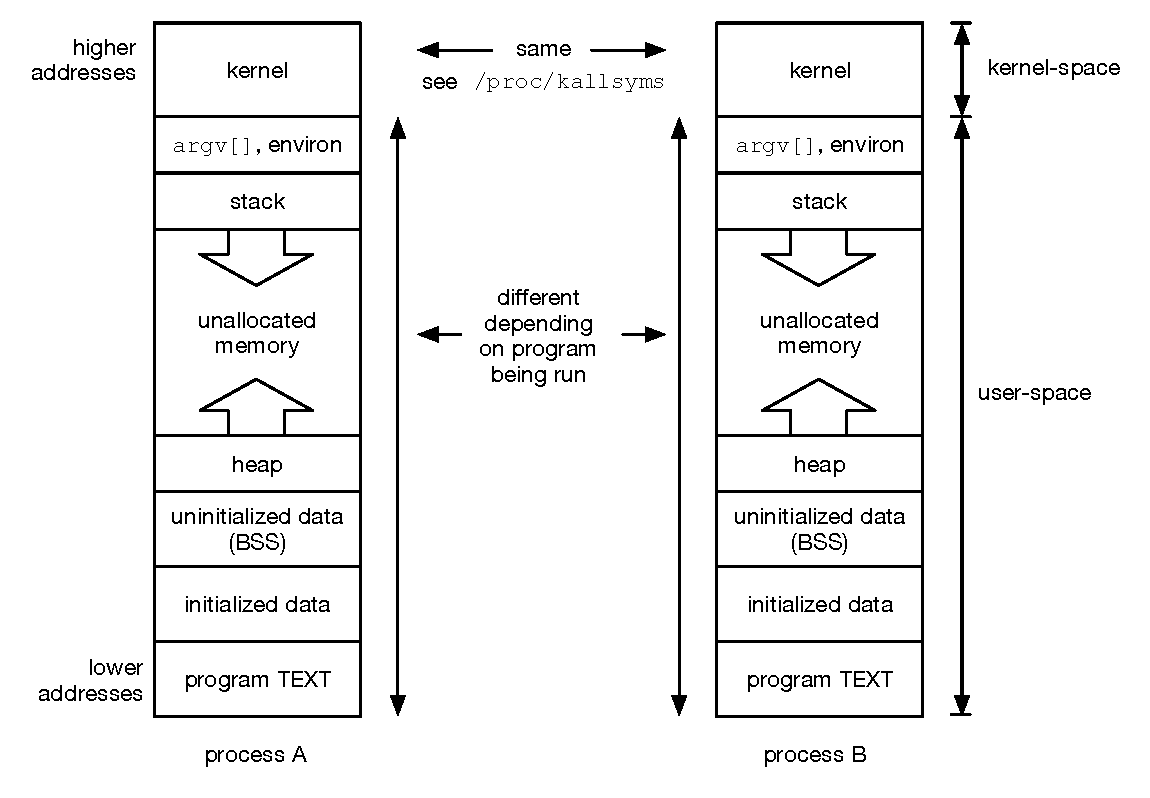
\includegraphics[scale=0.6]{figures/process-address-space.pdf}
	\centering
	\caption{Process address space showing user-space and kernel-space}
	\label{fig:process-address-space}
\end{figure}
 
It would be fun to explore the process address space here in more detail but that's a topic for another book or blog post. In short, just recognize that each process has its own, unique address space that is separate from all other processes, the kernel is mapped into all address spaces, user programs cannot access kernel addresses directly but can enter the kernel intentionally by invoking a system call.

%%%%%%%%%%%%%%%%%%%%%%%%%%%%%%%%%%%%%%%%%%%%%%%%%%%%%%%%%%%%%

\section{The System Call Interface}\label{syscalls}

This section shows how applications enter the kernel through invoking \textit{system calls}. The goal is to give readers a good place to start exploring execution paths through the kernel in response to familiar system calls that a program invokes such as \cf{open(2)}, \cf{read(2)} and \cf{stat(2)}.

A \textit{system call handler} is nothing more than a C function that operates in kernel space and calls other functions as needed. But the means of getting to this C function is somewhat complex and depends on the architecture on which the program is running. Consider figure \ref{fig:syscall-kernel} which shows the path from a everyone's favorite "\textit{Hello world!}" C program which calls \cf{printf(3)} which ends up in a call to the \cf{ksys\_write()} system call handler in the kernel. The program calls the standard library routine \cf{printf(3)} which in turn will invoke the \cf{write(2)} system call in order to write the string "\cf{hello world\textbackslash n}" to \cf{stdout}.

\begin{figure}
	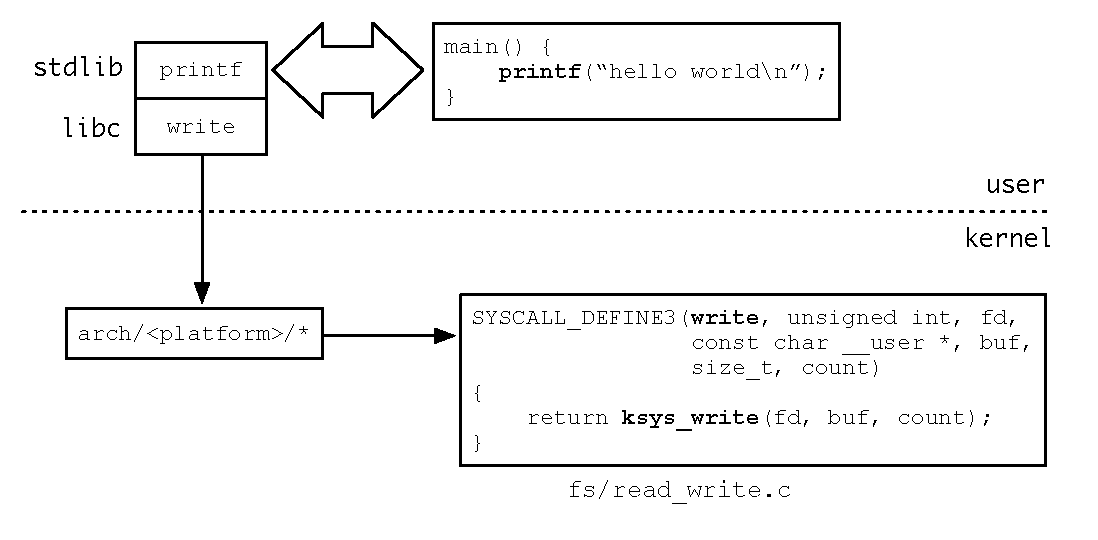
\includegraphics[scale=0.6]{figures/syscall-kernel.pdf}
	\centering
	\caption{Entering the kernel through the \cf{write(2)} system call}
	\label{fig:syscall-kernel}
\end{figure}

The details of how system calls are handled on each architecture won't be described in detail here but what follows are the steps taken on the x86\_64 architecture by the standard library (\cf{libc}) to enter the kernel for our "\cf{printf(Hello world!$\backslash$n");}" program. Arguments are passed into the kernel via CPU registers. If there are more than six arguments, the remaining arguments as pushed onto the stack.

\begin{quote}
- Store "1" in \cf{\%rax} ("1" is the system call number for the "write" system call)

- Store argument 1 in \cf{\%rdi} (in this case it will be "1" for \cf{stdout})

- Store argument 2 in \cf{\%rsi} (a pointer to the string "\cf{hello world\textbackslash n}")

- Store argument 3 in \cf{\%rdx} (the length of the string "\cf{hello world\textbackslash n}")

- Call the x86\_64 instruction "\cf{syscall}" to enter the kernel
\end{quote}

\noindent
For the Intel architecture, in the directory \cf{arch/x86/entry/syscalls}, there are two files which contain system call tables for both the 32-bit and 64-bit architectures. These files are \cf{syscall\_32.tbl} and \cf{syscall\_64.tbl} respectively. Here are the first few lines of \cf{syscall\_32.tbl}:

\begin{lstlisting}
0   i386    restart_syscall sys_restart_syscall
1   i386    exit            sys_exit
2   i386    fork            sys_fork
3   i386    read            sys_read
4   i386    write           sys_write
\end{lstlisting}

\noindent
You can see \cf{sys\_write} has the value of "4" which is different to the x86\_64 example above. On contrast, here are the first few lines of \cf{syscall\_64.tbl} for which the \cf{write(2)} system call is at position "1":

\begin{lstlisting}
0   common  read            sys_read
1   common  write           sys_write
2   common  open            sys_open
3   common  close           sys_close
4   common  stat            sys_newstat
\end{lstlisting}

\noindent
For further details on how system calls on x86 are handled I'd recommend reading the \textit{0xax} article "\textit{System calls in the Linux kernel. Part 1.}":

\begin{table}[h]
\begin{tabular}{lcl}
\parbox[r]{0.5in}{
\includegraphics[scale=0.15]{figures/url.png}} & \parbox[l]{0.55in}{URL \arabic{urls}} & \parbox[l]{3in}{\cf{https://tinyurl.com/rb3z8kds}}
\end{tabular}
\end{table}
\stepcounter{urls}
% https://0xax.gitbooks.io/linux-insides/content/SysCall/linux-syscall-1.html

\noindent
which explains how system calls are handled on the x86 platform in great detail. It shows an assembler version of "\textit{Hello world}", describing the path through to the architecture-specific areas of the kernel and into the C system call handling functions. 

\subsection{System Calls for File / Filesystem Activity}

There are a lot of system calls, in fact 322 for x86\_64 and 358 for x86. How many of these are related to filesystem activity? File / filesystem related system calls can be found in the \cf{fs} directory at the top level of the Linux kernel source tree. To get a rough idea of the number of file / filesystem related system calls, head into the \cf{fs} directory and run the following:

\begin{lstlisting}
$ [*\bfseries grep SYSCALL\_DEFINE3 *c | wc -l *]
56
\end{lstlisting}

\noindent
The actual number is a little less but this should help you get an idea of how many file / filesystem operations the kernel supports for applications.

Generally speaking, the easiest way to find the specific functions is to run "\cf{grep}" and you'll see that the file/filesystem functions are spread across 16 files. Here are some examples where \cf{grep} is run to look for specific function calls.

\begin{lstlisting}
$ [*\bfseries grep 'SYSCALL\_DEFINE3(write' *.c*]
read_write.c:SYSCALL_DEFINE3(write, unsigned int, fd, ...
read_write.c:SYSCALL_DEFINE3(writev, unsigned long, fd, ...
$ [*\bfseries grep 'SYSCALL\_DEFINE3(read' *.c *]
read_write.c:SYSCALL_DEFINE3(read, unsigned int, fd, ...
read_write.c:SYSCALL_DEFINE3(readv, unsigned long, fd, ...
stat.c:SYSCALL_DEFINE3(readlink, const char __user *, path, ...
$ [*\bfseries grep 'SYSCALL\_DEFINE3(fcntl' *.c*]
fcntl.c:SYSCALL_DEFINE3(fcntl, unsigned int, fd,  ...
fcntl.c:SYSCALL_DEFINE3(fcntl64, unsigned int, fd, ...
fcntl.c:COMPAT_SYSCALL_DEFINE3(fcntl64,  ...
fcntl.c:COMPAT_SYSCALL_DEFINE3(fcntl, unsigned int, fd, ...
\end{lstlisting}

\noindent
Most of these top-level functions don't do a great deal other than call other kernel functions. For example, in the case of the \cf{write(2)} system call, a call is made to \cf{ksys\_write()} as follows:

\begin{lstlisting}
SYSCALL_DEFINE3(write, unsigned int, fd, const char __user *, 
                buf, size_t, count)
{
    return ksys_write(fd, buf, count);
}
\end{lstlisting}

\noindent
There are 76 source code files in the \cf{fs} directory and over 90,000 LOC but the names of the files generally give a good hint as to what functionality they provide. For example:

\begin{itemize}
	\item \cf{open.c} -- contains source code for the \cf{open(2)} system call and other operations generally associated 
		with opening a file such as  \cf{ftruncate(2)} and the different file ownership change system calls 
		(\cf{chown(2)}, \cf{lchown(2)} etc), 
	\item \cf{read\_write.c} -- the code for \cf{read(2)}, \cf{write(2)} and vectored read / write system calls.
	\item \cf{readdir.c} -- system calls for reading directories including \cf{getdents64(2)}.
\end{itemize}

\noindent
There are several ways to browse through the kernel source but the best way will depend on your own personal preferences. Some people are happy with "\cf{cd}" and "\cf{grep}" but there are several tools that can help or at least give different options. Three such tools will be described in the following sections.

\subsection{Using \cf{vim} and \cf{ctags} to Browse the Kernel Source}

I remember the first time a colleague looked at me in surprise and said "\textit{You don't use tag stacking?}". I learned very quickly and have been using it for 30 years now. Most editors can make use of \cf{ctags(1)} but the program was originally built several decades ago to be used with \cf{vi(1)}.  What are ctags? From the manpage:

\begin{quote}
\textit{The ctags and etags programs (hereinafter collectively referred to as
       ctags, except where distinguished) generate an index (or "tag") file for
       a variety of language objects found in file(s).  This tag file allows
       these items to be quickly and easily located by a text editor or other
       utility. A "tag" signifies a language object for which an index entry is
       available (or, alternatively, the index entry created for that object).}
\end{quote}

\noindent
The following example generates a tags file for the whole of the Linux kernel source code. To do this, simply head to the top level directory of the source code and run the "\cf{ctags}" command:

\begin{lstlisting}
$ [*\bfseries cd linux-6.3.3*]
$ [*\bfseries ctags -R **]
\end{lstlisting}

\noindent
This will create a very large file (for the 6.3.3 sources it's 1,067,091,840 bytes - ouch!).

Once you have the tags file, navigate to the top level Linux source tree and enter your favorite editor using the option to specify a tag. In \cf{vi} pass the \cf{-t} option together with the function or global variable that you're looking for. The following command will open \cf{vi} in \cf{fs/read\_write.c} with \cf{ksys\_write()} in the center of the screen.

\begin{lstlisting}
$ [*\bfseries vi -t ksys\_write*]
\end{lstlisting}

\noindent
Note that you need to be in the directory where the tags file is located. You can also search for global variables too so:

\begin{lstlisting}
$ [*\bfseries vi -t file\_systems*]
\end{lstlisting}

\noindent
will open \cf{vi} in \cf{fs/filesystems.c} at the place where the \cf{file\_systems} global variable is defined.

I typically have this one-liner in my \cf{.bashrc} file:

\begin{lstlisting}
alias linux='cd ~/src/linux-6.3.3 ; pwd'
\end{lstlisting}

\noindent
to get me to the top of the current source tree that I'm using. I can then run "\cf{vi -t}" to enter the file at the place I want.

Another option is to build a little script that displays various routines. The following script switches to the top of the kernel source tree where it assumes you have a tags file and then enters \cf{vi} using a tag that you choose. The advantage here is that once inside the file, you can now use tag stacking to move through the kernel source from one function to another. 

Here is a shorter version of the \cf{bash} script. It's very simple and obviously you can put any function or global variable in here.

\begin{lstlisting}
TAGS_DIR=~/src/linux-6.3.3

echo "
1 - open
2 - read
3 - write
4 - readlink

a - task_struct
b - super_operations

q - quit
"

cd $TAGS_DIR
while :
do
    /bin/echo -n "System call? "
    read choice
    case $choice in
        1) vi -t do_sys_open ;;
        2) vi -t ksys_read ;;
        3) vi -t ksys_write ;;
        4) vi -t do_readlinkat ;;
        a) vi -t task_struct ;;
        b) vi -t super_operations ;;
        q) break ;;
        *) echo "Invalid choice"
    esac
done
\end{lstlisting}

\noindent
Now that you can get in to a file at the location of the system call handler you've been looking for, it's time to cover how tag stacking works so you can search through the code from one function to the next. Regardless of where you are in the file, if you want to go to the location of the tag where the cursor points to and then back again to the current file and location, use the following two commands in order:

\begin{itemize}
	\item \cf{Ctrl + ]} -- Move to the file where the tag under cursor is located (function, global variable etc). This is 
		identical to running "\cf{vi -t}"  specifying the tag name from the command line.
	\item \cf{Ctrl + t} -- Move back to the previous file/position.
\end{itemize}

\noindent
For example, in figure \ref{fig:tag-stacking} we entered this file with "\cf{vi -t ksys\_write}" and the cursor is on
the function name \cf{vfs\_read()}. By hitting "\cf{Ctrl + ]}", \cf{vi} will take you to the location of \cf{vfs\_read()}. It happens to be in the same file but if it was a different file, you'd enter that file instead. If you then hit "\cf{Ctrl + t}" you will go back to the file/location where you started.

\begin{figure}
	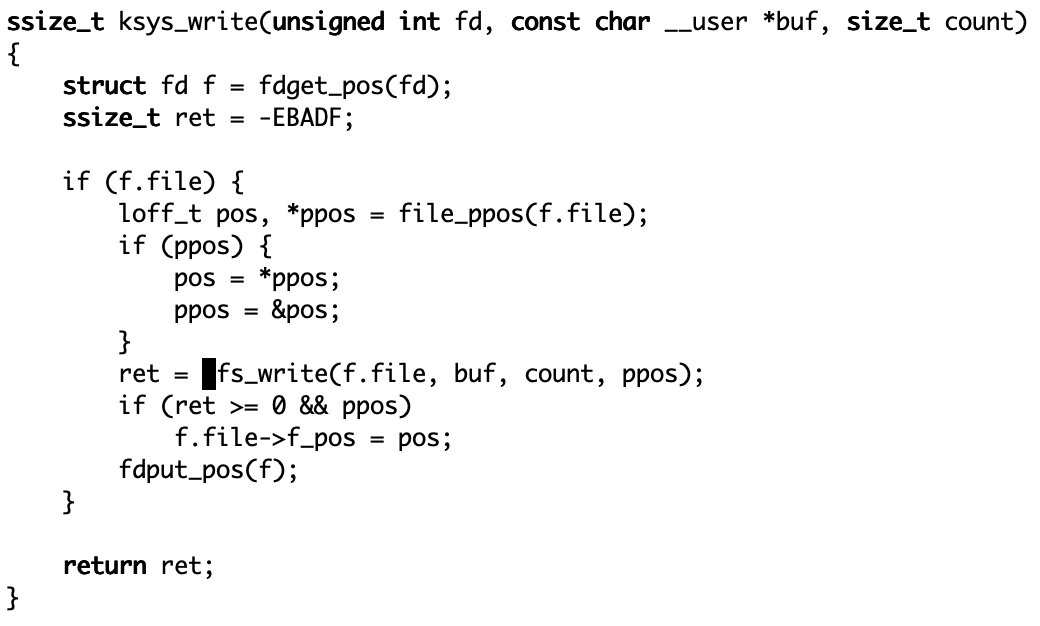
\includegraphics[scale=0.6]{figures/tag-stacking.png}
	\centering
	\caption{Using tag-stacking to navigate through the kernel source code}
	\label{fig:tag-stacking}
\end{figure}

The current tag stack is the list of all places in the source tree you have moved to through repeated calls to "\cf{Ctrl + ]}". You can view the current tag stack by typing "\cf{:tags}" in \cf{vi}. See figure \ref{fig:tag-stacking-2} for an example. This shows going from \cf{vi -t ksys\_write} to \cf{vfs\_read()} and then to \cf{rw\_verify\_area()}.

\begin{figure}[h]
	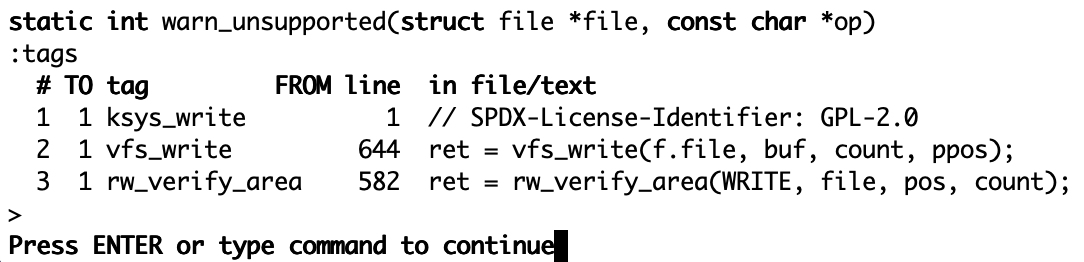
\includegraphics[scale=0.6]{figures/tag-stacking-2.png}
	\centering
	\caption{Current tag stack}
	\label{fig:tag-stacking-2}
\end{figure}

I've tried some of the newer editors and have struggled to move around files as quickly as I can with \cf{vi} and tag stacking.

\subsection{Using \cf{cscope} to Browse the Kernel Source}

Another excellent tool to use, especially in conjunction with \cf{vi} and tag stacking, is the \cf{cscope(1)} command which has been around since the early 1980s. It's a tool I've used for over thirty years and have used extensively while writing this book. Notes about the early history of \cf{cscope} can be found here:

\begin{table}[h]
\begin{tabular}{lcl}
\parbox[r]{0.5in}{
\includegraphics[scale=0.15]{figures/url.png}} & \parbox[l]{0.55in}{URL \arabic{urls} -- } & \parbox[l]{3in}{\cf{https://tinyurl.com/ywce8h9n}}
\end{tabular}
\end{table}
\stepcounter{urls}
% https://cscope.sourceforge.net/history.html

I particularly enjoyed reading the goals behind starting the project:

\begin{quote}
\textit{Joe Steffen first started writing cscope in the early 1980's as an aid for his own work. It started as little more than a set of shell scripts containing greps and seds. It became clear to Joe that this was not going to work on large projects (say, more than 20 or so files, which was a large project on a PDP-11!) as most of the time consumed was in parsing the C source code over and over again. So he wrote a C program that did the grunt work of parsing into a tagged database, and then presented the screen with common searches. The tagged database was updatable and saved between sessions. Productivity soared!}
\end{quote}

\noindent
Imagine that -- a project with 20 or so files? Today, the Linux kernel source tree now has close to 26 million files. Of course \cf{grep} is still very useful so some things don't change.

History lesson beside, the first time you run \cf{cscope} you will need to generate the cross-reference database as shown below. The command must be run from the top kernel source directory:

\begin{lstlisting}
$ [*\bfseries cd linux-6.3.3*]
$ [*\bfseries cscope -Rk **]
\end{lstlisting}

\noindent
Since the kernel source is quite large, this takes quite a while and the database comes in at over just over 1 GB. Thus you'll need over 2 GB of free space for using "\cf{cscope}" and "\cf{ctags}". The "\cf{R}" option instructs \cf{crash} to recurse through all directories and the "\cf{k}" option (Kernel Mode) will turn off using the default include directory (\cf{/usr/include}) when building the database, since when building the kernel, these include files won't be used. Only header files within the kernel source tree are used since header files in \cf{/usr/include} will likely be for a different kernel release. In the Linux source tree, the \cf{include} directory used during kernel builds is at the top level of the source tree. 

Once the database has been generated or on subsequent runs, you will see output similar to what is shown in figure \ref{fig:cscope-1}. The \cf{cscope} version will be displayed at the top of the screen together with a note to let you know that you can press "\cf{?}" at any time to get help:
 
 \begin{figure}[h]
	\centering
	\includegraphics[scale=0.6]{figures/cscope-1.png}
	\caption{The main \cf{cscope} screen}
	\label{fig:cscope-1}
\end{figure}

Everything is set up such that the cursor is on the line where you can search for a symbol so all you have to do is enter the symbol you are looking for and press the return key. For example, after typing "\cf{ksys\_read}" and pressing "RETURN", the results will be displayed at the top of the screen as shown in figure \ref{fig:cscope-2}.

\begin{figure}
	\centering
	\includegraphics[scale=0.6]{figures/cscope-2.png}
	\caption{The \cf{cscope} results of searching for \cf{ksys\_read}}
	\label{fig:cscope-2}
\end{figure}

For each search item displayed you can press the number key shown on the left-hand-side to enter the file at that location. In this example, press '\cf{2}' to enter \cf{read\_write.c} at the location where the function \cf{ksys\_read()} is located. Or you can use the arrow keys to move between items displayed and just press "RETURN". If there are more items than can be displayed on a single screen, use the space bar to go to subsequent screens. The "TAB" key toggles between the search results and the menu at the bottom of the screen. "\cf{Ctrl + d}" exits \cf{cscope}. 

While in menu mode, if you use the arrow keys to move down to "\cf{Find this global definition}", type \cf{ksys\_read} and press the return key, \cf{cscope} will locate the symbol and enter the file at the correct location. If you are looking for a function that is called by many other functions, the list of hits at the top of the screen could be several pages long. Searching for the global definition can save time searching.

Next time you run \cf{cscope} just add the \cf{-d} option to instruct it not to regenerate the database again. Unless of course some of the source code files have changed. If the database needs to be generated again, it should be faster than the first time it's generated.

Now the best part of using \cf{cscope} is to combine it with your favorite editor and use tag stacking. Then you have the best of all worlds since you can search easily, locate the function of your choice and move down through functions it calls.

%------------------------------------------------------------------------------------------------------------------------------------------------------------------

\subsection{Using Elixir to Browse the Kernel Source}

Elixir is a cross reference tool for the Linux source code hosted by embedded Linux provider Bootlin. It doesn't just support a specific version of the kernel but every version that exists all the way back to day one and up to the most recent development kernels. Everyone has their own way of navigating through source code using their favorite editor and using tools such as \cf{ctags} but sometimes it's nice just scroll through a page of source code using the mouse. You can find Elixir by pointing the browser to \cf{elixir.bootlin.com} to get to the latest sources or using the following link. Alternatively just search for "elixir linux" in your favorite browser.

\begin{table}[h]
\begin{tabular}{lcl}
\parbox[r]{0.5in}{ \includegraphics[scale=0.15]{figures/url.png}} & \parbox[l]{0.1in}{\arabic{urls}} & \parbox[l]{3in}{\cf{https://tinyurl.com/447v7urs}}
\end{tabular}
\end{table}
\stepcounter{urls}
% https://elixir.bootlin.com/linux/latest/source

\noindent
Figure \ref{fig:elixr-1} shows an example of using Elixir and displaying the results of searching for the symbol \cf{ksys\_write}. In this example, we are searching through the 6.1.4 source code tree. You can change which Linux kernel version to search by selecting the version on the left hand side of the screen.

\begin{figure}
	\includegraphics[scale=0.4]{figures/elixr-1.png}
	\centering
	\caption{Elixir search for the function \cf{ksys\_write}}
	\label{fig:elixr-1}
\end{figure}

Figure \ref{fig:elixr-2} shows the source code for our symbol. As well as typing the name of something to search for in the \textit{All symbols} search bar you can also click on function names and global variables when the source code is being displayed.

\begin{figure}
	\includegraphics[scale=0.4]{figures/elixr-2.png}
	\centering
	\caption{Elixir displaying the source code for the selected function}
	\label{fig:elixr-2}
\end{figure}

You can also use Elixir on other source code projects including \cf{glibc}. Just click the arrow on the right hand side of "Linux" towards the top left of the page and a number of other projects will be displayed.


%------------------------------------------------------------------------------------------------------------------------------------------------------------------

\subsection{Maintaining Your Own Notes}

Of course you don't need to rely on all of the tools shown here for browsing the kernel source. You will develop your own methods of browsing the kernel source over time based on your preferences. How you keep notes is also a matter of personal choice. I have a directory of simple text files that I use \cf{vi} to add notes. You may wish to maintain one using rich-text or some other format.

I also have a file called "structures" which contains a copy of all of the Linux kernel structures that I typically look at. Even while browsing with \cf{vi} or Elixir, I'm usually following a code path and like to have the file close by for easy searching. It looks like this:

\begin{lstlisting}
------------------------------------------------------------

mount - fs/mount.h

    struct mount {
        struct hlist_node        mnt_hash;
        struct mount            *mnt_parent;
        struct dentry           *mnt_mountpoint;
        struct vfsmount          mnt;
        ....
    
------------------------------------------------------------

vfsmount - include/linux/mount.h

    struct vfsmount {
        struct dentry         *mnt_root;    
        struct super_block    *mnt_sb;   
        ....
\end{lstlisting}

\noindent
I've even formatted the structures to make it visibly easy to read since most of the Linux header files are full of compiler directives and \cf{\#ifdef}s which make the code harder to read. Searching for structures is also easy. I use "\cf{/\^{}vfsmount}" to search for "vfsmount" on the first line and that takes me right to the structure I'm looking for. You can do the same in your editor of choice.

I also use Omnigraffle on my Macbook Pro and have drawn a lot of code walkthrough figures, some of which can be found throughout the book. Perhaps pencil and paper or a tablet may be your choice of tool.

%%%%%%%%%%%%%%%%%%%%%%%%%%%%%%%%%%%%%%%%%%%%%%%%%%%%%%%%%%%%

\section{File Access Structures}

Now that you know where the filesystem code is located in the Linux kernel source tree and have some tools to navigate through the relevant filesystem system calls, we'll switch our focus to the main structures that are used for file / filesystem access. These structures are defined in the \cf{include} directory at the top of the Linux kernel source tree. The following sections will reference the relevant fields of each structure as each structure is explained but not all of the fields of each structure will be described. For some structures, there are many fields and describing them all here will just be overload and will inhibit  understanding how they are used. Other fields will be introduced as needed throughout subsequent chapters. 

To get started, consider figure \ref{fig:per-file-kernel-structures} which shows how the main structures in the kernel used for accessing files are linked together. It all starts with the \cf{task\_struct} structure, for which there is one such structure per process. 

In this figure there are some structures that are per-process only and some that are shared between all processes as indicated by the dotted line. For example, for every open file, each process needs its own file offset for reading and writing together with specific flags that it has set during an open call. This is where the \cf{file} struct comes into play. However, there may be multiple processes accessing the same file simultaneously so, although each process has distinct \cf{file} structures, they all share a common \cf{inode} structure for the file in question.

\begin{figure}[h]
	\centering
	\includegraphics[scale=0.6]{figures/per-file-kernel-structures.pdf}
	\caption{Kernel structures for accessing open files}
	\label{fig:per-file-kernel-structures}
\end{figure}

%----------------------------------------------------------------------------------------------------------------------------------------------------------------

\subsection{File Descriptors}

File access starts with a file descriptor that a process gets back from \cf{open(2)} and friends. In older versions of UNIX, the file descriptor was an index into an array of pointers to "\cf{struct file}" elements held within the \cf{u\_area} structure which in turn referenced a \cf{proc} structure, similar to the Linux \cf{task\_struct}. This allowed for a fixed number of open files, a restriction that continued through to SVR3 UNIX into the early 1990s. At SCO, although we had an SVR3-based version of UNIX at the time, the limit was removed to allow for a more dynamic (and tunable) number of open files. 

This hard limit was similar in the first version of Linux which had the following field in the \cf{task\_struct} structure:

\begin{lstlisting}
struct file * filp[NR_OPEN];
\end{lstlisting}

\noindent
with \cf{NR\_OPEN} defined as 20. This meant that there was a hard coded limit of 20 open files. For most processes that's still reasonable since in a standard Ubuntu running instance, there are a relatively small number of processes with over 20 open files. 

Using a file descriptor as an index into an array pointing to \cf{file} structures was the reason that \cf{stdin}, \cf{stdout} and \cf{stderr} originally had the values of 0, 1 and 2 respectively. These numbers were used to access the first 3 elements of the file descriptor array. Regardless of how an operating system may implement POSIX file access, this convention remains intact today.

Handling file descriptors in Linux is similar today although the implementation has become more complex when handling large numbers of open files, the details of which will be described later in section \ref{fdalloc}. To get started, there are three fields in the \cf{task\_struct} which have relevance to files, filesystems and namespaces:

\begin{lstlisting}
struct task_struct {
    struct fs_struct    *fs;      /* Filesystem information: */
    ...
    struct files_struct *files;   /* Open file information: */
    ...
    struct nsproxy      *nsproxy; /* Namespaces: */
}
\end{lstlisting}

\noindent
Filesystems and namespaces will be described later but for file access, the \cf{files} field is a pointer to a \cf{files\_struct} structure for which the most relevant fields are:

\begin{lstlisting}
struct files_struct {
    struct fdtable __rcu *fdt;
    unsigned int          next_fd;
    ...
}
\end{lstlisting}

\noindent
The \cf{next\_fd} field contains the number of the next file descriptor that will be allocated. For a new process this will be 3 which is 1 above \cf{stderr}. The \cf{fdt} field points to an \cf{fdtable} structure.

%----------------------------------------------------------------------------------------------------------------------------------------------------------------

\subsection{The \cf{fdtable} Structure}

\begin{lstlisting}
struct fdtable {
    unsigned int        max_fds;
    struct file __rcu **fd;             /* current fd array */
    unsigned long      *close_on_exec;
    unsigned long      *open_fds;
    unsigned long      *full_fds_bits;
};  
\end{lstlisting}

\noindent
\textbf{Given a file descriptor, this is an efficient way to get to the \cf{file} structure in most instances. Just index into the \cf{fd} array. --- need to look to see how it works. If the fd is small and there is only one table, it's easy. If it's a larger number, can it uses the current fd array or not? Need to look}. Therefore Linux has made it efficient to handle a small number of open files while still being extensible to support a much larger number.

The \cf{max\_fds} field is set to 256 but this is just the number of file descriptors that a process can have initially and, as discussed, for most processes, this will suffice. We'll cover how greater numbers of file descriptors are managed later in section \ref{fdalloc}. It's become somewhat messy in Linux today but involves allocation of multiple \cf{fdtable} structures. \textbf{XXX -- reword all this once that work is complete}

There is one file descriptor per open instance which results from a call to \cf{open(2)}, \cf{creat(2)} for example. The \cf{file} structure however can be shared by multiple open instances (more than one file descriptor). This is achieved by calling \cf{dup(2)} which will return a new file descriptor. In this case there will be two entries in the file descriptor array (one per file descriptor) but both will point to the same \cf{file} structure.

%----------------------------------------------------------------------------------------------------------------------------------------------------------------

\subsection{The \cf{file} Structure}

The \cf{file} structure has some fields that correspond to the arguments to \cf{open(2)} call such as \cf{f\_flags} and \cf{f\_mode} as well as subsequent operations such as \cf{read(2)}, \cf{write(2)} and \cf{lseek(2)}: \textbf{XXX -- check on flags and mode when going through open code}

\begin{lstlisting}
struct file {
    struct path        f_path;   
    struct inode       f_inode;  
    atomic_long_t      f_count;  
    unsigned int       f_flags;  
    fmode_t            f_mode;   
    loff_t             f_pos;    
    struct fown_struct f_owner;  
    const struct cred  f_cred;   
    ....
}
\end{lstlisting}

\noindent
Exploring these fields:

\begin{itemize}
	\item \cf{f\_path} -- contains a pointer to the dcache dentry for this file as well as the filesystem to which this file belongs. 
		The dcache allows for fast lookups to get to a file when system calls such as \cf{open(2)} pass a pathname to search. 
		To access the file's name, the field \cf{f\_path.dentry->d\_name.name} can be used. The dcache will be described 
		below in section \ref{kstruct-dcache}.
	\item \cf{f\_inode} -- the corresponding Linux inode for the file. There may be multiple references
		to a file within a single process or from multiple processes but there will only be one Linux inode. Inodes are
		described in section \ref{inodes}.
	\item \cf{f\_count} -- a reference count for the number of file descriptors that reference  this \cf{file} structure. 
		If we open a file for the first time, \cf{f\_count} will be 1. If we then call \cf{dup(2)}, we have two file descriptors 
		referencing this same \cf{file} structure so the reference count will be 2. We'll demonstrate reference counts later on.
	\item \cf{f\_flags} -- the open flags which were passed to \cf{open(2)} and other system calls. 
	\item \cf{f\_mode} -- {\bf this is essentially the \cf{mode} argument}.
	\item \cf{f\_pos} -- The position within the file that will be used for the next \cf{read(2)} or \cf{write(2)} system call. This 
		field can also be changed by a call to \cf{lseek(2)}.
	\item \cf{f\_owner} -- {\bf XXX---TBD}
	\item \cf{f\_cred} -- {\bf the process user credentials for this file open}
\end{itemize}

\noindent
How and when these fields are changed will be described in more detail in the section \ref{openfile} when describing the flow through various system calls.

\begin{table}[h]
\begin{tabular}{ll}
\parbox[l]{0.6in}{\includegraphics[scale=0.8]{figures/src-xref.pdf}} & \parbox[l]{4in}{\small{Most of the structures described in this section can be found in the header file \cf{include/linux/fs.h}}}
\end{tabular}
\end{table}

\noindent
You will see references to this header file throughout the book. It contains many structures that are related to file and filesystem access.

%----------------------------------------------------------------------------------------------------------------------------------------------------------------

\subsection{The \cf{inode} Structure}

Section \ref{kstruct-inodes} describes the inode cache and the relationship between in-core inodes and disk-based inodes. To complete this section in terms of how the main structures all link together, an \textit{inode} is the in-core representation of an open file. For each file that is open, regardless of whether it is on local disk, RAM or over the network, there will be a Linux inode in-core represented by the \cf{inode} structure.

As file I/O takes place for regular files, the inode references a \textit{page cache mapping} which in turn references cached pages in memory. This is shown in figure \ref{fig:kstruct-inode-pages}.

\begin{figure}[h]
	\includegraphics[scale=0.6]{figures/kstruct-inode-pages.pdf}
	\centering
	\caption{The Linux \cf{inode} which references data cached in memory}
	\label{fig:kstruct-inode-pages}
\end{figure}

\noindent
Although there may be multiple \cf{file} structures in memory representing different open instantiations of the same file from different processes, there will only be one \cf{inode} structure which is shared across all processes. File I/O and locking together with the internal operation of the inode cache will be described in section \cf{vfs-inode-cache}.

%%%%%%%%%%%%%%%%%%%%%%%%%%%%%%%%%%%%%%%%%%%%%%%%%%%%%%%%%%%%%%%%

\section{The Directory Cache}\label{kstruct-dcache}

Consider the simple command:

\begin{lstlisting}
$ [*\bfseries ls /home/spate/spfs/kern/spfs.ko*]
\end{lstlisting}

\noindent
To perform this operation, called \textit{pathname resolution}, the \cf{ls(1)} command calls the \cf{statx(2)} system call passing the pathname supplied as an argument. When parsing this pathname, the kernel has to process five different directories starting with "\cf{/}" and ending with "\cf{kern}".  As the path is being processed, it must validate that each directory in the path not only exists but that the caller has permission to access the directory. A permissions check is also performed on the base file. In this example, information about the regular file "\cf{spfs.ko}" is returned through a \cf{stat} structure. For an \cf{open(2)} call, the kernel finishes by setting up the structures described in the previous section and returning a file descriptor.

Each component of the pathname is represented by an \textit{inode} in a local filesystem or other entity over the network for filesystems such as NFS. Every time a call is made to the access a directory inside the filesystem, there can be many calls to read structures from disk which which is a time-consuming operation.  Accessing the same files happens frequently therefore minimizing disk access is imperative to improving the performance of the system. This is where the Linux \textit{dcache} (directory cache) comes into play. The dcache is a variation of the \textit{Directory Name Lookup Cache} (DNLC) which has been around for several decades now and was first introduced in BSD UNIX to solve the the \textit{pathname resolution} problem.

The Linux directory cache (simply called the \textit{dcache}) has the same goal as the original DNLC which is to provide a fast and efficient method of mapping any file name to a Linux inode regardless of the type of file. While resolving a pathname component for the first time, the kernel will ask the filesystem to lookup a filename within a specific directory. Once the filesystem locates this file, a reference to it can be stored in the dcache so that a subsequent lookup does not need to go to disk. Over the time, for frequently accessed files, the goal is to read from the dcache as much as possible. It is generally possible to get a dcache hit ratio of 80\% or higher.

%---------------------------------------------------------------------------------------------------------------------------------------------------------------------

\subsection{Introducing The \cf{dentry} Structure}

The main structure that underpins the dcache is the \cf{dentry} (directory entry). Dcache entries are searched using the parent directory dentry and a string for the file that is being searched for.

 \begin{table}[h]
\begin{tabular}{ll}
\parbox[l]{0.6in}{\includegraphics[scale=0.8]{figures/src-xref.pdf}} & \parbox[l]{4in}{\small{The \cf{dentry} structure can be found in the \cf{include/linux/dcache.h} header file together with the global variable \cf{dentry\_hashtable} which references the dcache hash buckets.}}
\end{tabular}
\end{table}

 \noindent
 For each file that is present in the Linux dcache there is a dentry. After resolving the path "\cf{/mnt/file-a}", there are dentries in teh dcache for "\cf{/}", "\cf{mnt}" and "\cf{file-a}". Note that the dentry for "\cf{/}" will actually be present in the dcache from early in the boot process.
 
If the file "\cf{/mnt/file-a}" also has a hard link accessible via "\cf{/path-to-file-a}" and both entries are in the dcache, there will be two distinct dentries, one for "\cf{file-a}" and one for "\cf{path-to-file-a}".

Here are the basic set of \cf{dentry} fields. Others will be covered in later sections as the further details of the dcache are explored.

\begin{lstlisting}
struct [*\bfseries dentry*] {
    unsigned int                    d_flags;
    struct dentry                  *d_parent; 
    struct qstr                     d_name;
    unsigned char                   d_iname[DNAME_INLINE_LEN];    
    struct inode                   *d_inode;
    const struct dentry_operations *d_op;
    struct super_block             *d_sb;   
    struct hlist_bl_node            d_hash;
    struct list_head                d_lru; 
    struct list_head                d_child;    
    struct list_head                d_subdirs;  
    unsigned long                   d_time;  
    ...
}
\end{lstlisting}

\noindent
For the structure fields that are shown above, here is a general overview of their purpose:

\begin{itemize}
	\item \cf{d\_flags} -- there are a lot of flags. A few will be discussed below and others introduced as needed 
		throughout this section and in section \ref{vfs-dcache}.
	\item \cf{d\_parent} -- a pointer to the dentry for the parent directory.
	\item \cf{d\_iname} -- this field holds the name of the file if the size of the file name is less than 
		(\cf{DNAME\_INLINE\_LEN - 1}) bytes.
	\item \cf{d\_name} -- for small file names, the \cf{name} field within this \cf{qstr} structure will point to the \cf{d\_iname} field
		described above. For file names that are \cf{DNAME\_INLINE\_LEN} and longer, memory is allocated 
		and this field will point to the allocated memory where the file name is then stored.
	\item \cf{d\_inode} -- this field points to the Linux inode representing the underlying file. If the file doesn't exist, this
		field is set to \cf{NULL} and the dentry is known as a \textit{negative dentry}. Just as with files that exist, 
		negative dentries are useful to prevent repeated filesystem lookups.
	\item \cf{d\_op} -- filesystems can override / provide their own dcache functions that are called by the dcache when 
		performing specific operations. For local filesystems the dcache is expected to be a correct representation of 
		what's on disk but for network filesystems, a call may be needed to validate specific dentries since the cache
		may be out of date with respect to the server. This is because other clients may have made changes to a file
		making the dcache on this node out of date.
	\item \cf{d\_sb} -- the filesystem to which these dentries belong. This is particularly important during unmount
		and when pruning the dcache to reduce its memory footprint by getting easy access to all dentries for a 
		specific filesystem.
	\item \cf{d\_hash} -- the dcache itself is accessible through the \cf{dentry\_hashtable} global variable which is a large 
		collection of hash buckets. Which hash bucket to use is determined by calling the \cf{d\_hash()} function passing the 
		parent dentry and the file name. Each hash bucket can contain zero or more dentries linked through this field.
	\item \cf{d\_lru} -- all dentries that are not currently being accessed are collected on an LRU list linked through this 
		field. LRU lists are per filesystem and accessed through the \cf{s\_dentry\_lru} field of the \cf{super\_block} structure.
	\item \cf{d\_subdirs} /  \cf{d\_child} -- this field points to a list of dentries, one for each cached file within the directory 	
		referenced by this dentry. These child dentries are linked through \cf{d\_child}.
	\item \cf{d\_time} -- this field is only used by NFS and vboxfs to revalidate an entry after a specific time period has passed.
\end{itemize}

\noindent
The \cf{i\_dentry} field of the inode points to a list of dentries that reference this file. Note that there can be multiple links to the same file. For example:

\begin{lstlisting}
$ [*\bfseries touch /mnt/mydir/myfile*]
$ [*\bfseries ln /mnt/mydir/myfile link*]
\end{lstlisting}

\noindent
If the file were accessed using both paths there would be one inode for the actual file but two dentries, one for each file name. 

There are 35 different \cf{d\_flags} but not all flags will be covered in the book. A few are described below and other notable flags will be covered in section \ref{vfs-dcache} when the dcache implementation is described in more detail.

\begin{itemize}
	\item \cf{DCACHE\_MOUNTED} -- generally speaking, this flag is set on each dentry that has a filesystem mounted on 
		top of it.  Since Linux supports multiple filesystem namespaces, it is possible that the dentry may not be mounted 
		on in this namespace, therefore this flag is seen as a hint, not a guarantee.
	\item \cf{DCACHE\_LRU\_LIST} -- the dentry has no active holds and is therefore on the LRU list. It is quite possible
		that if the file is requested again, it will be found on this list before it is discarded.
	\item \cf{DCACHE\_REGULAR\_TYPE} -- this is a regular file. There are also flags for directories, symlinks 
		and special files.
	\item \cf{DCACHE\_NEED\_AUTOMOUNT} -- if the kernel needs to traverse into a directory for which this dentry flag
		is set, it has hit an auto-mount directory so an attempt is made to mount the remote filesystem before 
		pathname resolution can proceed.
	\item \cf{DCACHE\_REFERENCED} -- the dentry has recently been accessed and therefore it should not be discarded.
\end{itemize}

\noindent
There are seven flags that are set during dentry creation depending on whether the filesystem supports a list of \cf{dentry\_operations} (hanging off the \cf{s\_d\_op} field of the \cf{super\_block} structure). Most filesystems do not have such a list of operations but they are common for network filesystems. The flags can be found in \cf{dcache.h} by searching for \cf{DCACHE\_OP\_*}. For example, if the \cf{DCACHE\_OP\_COMPARE} flag is set when the kernel is looking up a file
in the dcache, a call is made into the filesystem to actually perform the comparison.

To show how the dentry structures are related, consider figure \ref{fig:kernel-pathname-tree} which shows a small file tree with a filesystem mounted on the directory \cf{mount-dir}.

\begin{figure}[h]
	\includegraphics[scale=0.6]{figures/kernel-pathname-tree.pdf}
	\centering
	\caption{A simple example file hierarchy}
	\label{fig:kernel-pathname-tree}
\end{figure}

For this particular tree, if we assume that all dentries are in the dcache, they are connected as shown in figure \ref{fig:kernel-pathname-dentries}. The figure shows the connection between the parent and child dentries through the \cf{d\_parent}, \cf{d\_subdirs} and \cf{d\_child} fields. Notice that there is no direct connection between the base filesystem and the filesystem that is mounted on \cf{mount-dir}. However, the \cf{DCACHE\_MOUNTED} mounted flag will generally be set on the dentry for \cf{mount-dir} indicating that the directory has been mounted on. \textbf{This isn't always true in the case of namespace which will be covered later.}

\begin{figure}[h]
	\includegraphics[scale=0.6]{figures/kernel-pathname-dentries.pdf}
	\centering
	\caption{dentries for the example file hiearchy}
	\label{fig:kernel-pathname-dentries}
\end{figure}

%------------------------------------------------------------------------------------------------------------------------------------------------------------------------

\subsection{Dcache Hash Buckets}

The Linux dcache is basically a large list of hash buckets and is accessed through the glocal \cf{dentry\_hashtable} variable:

\begin{lstlisting}
static struct hlist_bl_head *dentry_hashtable
\end{lstlisting}

\noindent
A simple example of how \cf{dentry\_hashtable} references the hash buckets is shown in figure \ref{fig:kernel-dentry-hashtable}. Each dentry in the cache is hashed using the dentry of its parent and the file name. To see if a file name is present in the cache, the kernel hashes to get the correct hash bucket then walks the appropriate list to look for the entry that it's searching for. Hash lists are generally fairly short, again helping with performance.


\begin{figure}[h]
	\includegraphics[scale=0.6]{figures/kernel-dentry_hashtable.pdf}
	\centering
	\caption{The dcache headed by \cf{dentry\_hashtable}}
	\label{fig:kernel-dentry-hashtable}
\end{figure}

Each element in the hash table is a pointer to a list of dentries that hash to the same value. The function \cf{d\_hash()} calculates the hash and thus gives access to the right hash bucket.

\begin{lstlisting}
static inline struct hlist_bl_head *
[*\bfseries d\_hash(unsigned int hash)*]
{
    return [*\bfseries dentry\_hashtable*] + (hash >> d_hash_shift);
}
\end{lstlisting}

\noindent
There is quite a lot of code behind hashing to locate the correct bucket. Section \ref{dcache-hash} covers the process in more detail. \textbf{XXX -- not sure it does but come back to this}.

%------------------------------------------------------------------------------------------------------------------------------------------------------------------------

\subsection{KGDB -- Analyzing The Dcache}

\textbf{XXX -- there is something wrong here. One entry in the left column and others the right column. Need to fix}

This example shows how to dump out part of the dcache hash table and view some of the dentries. The dcache is accessed through \cf{dentry\_hashtable} and each hash bucket is of the following type:

\begin{lstlisting}
struct [*\bfseries hlist\_bl\_node*] {
    struct hlist_bl_node *next, **pprev;
};
\end{lstlisting}

\noindent
Starting at \cf{dentry\_hashtable}, each bucket occupies two addresses (forward and back pointers). Here we display 24 addresses:

\begin{lstlisting}
(gdb) [*\bfseries x/24a dentry\_hashtable*]
0xffff88817b800000:    0x0                0x0     
0xffff88817b800010:    0x0                0xffff888103132248
0xffff88817b800020:    0x0                0x0
0xffff88817b800030:    0x0                0x0 
0xffff88817b800040:    0x0                0x0
0xffff88817b800050:    0x0                0x0 
0xffff88817b800060:    0x0                0x0
0xffff88817b800070:    0x0                0x0
0xffff88817b800080:    0x0                0x0
0xffff88817b800090:    0xffff888101a816c8 0x0
0xffff88817b8000a0:    0x0                0x0
0xffff88817b8000b0:    0x0                0xffff8881013a6788
\end{lstlisting}

\noindent
The first thing to notice and especially if you dump more addresses is that most buckets are empty. Taking the first address displayed, we need to call \cf{container\_of()} to get to the dentry since this list goes through the \cf{d\_hash} field of the dentry structure.

\begin{lstlisting}
(gdb) [*\bfseries set \$de = \$container\_of(0xffff888103132248, \textbackslash*]
                                      [*\bfseries "struct dentry", "d\_hash")*]
\end{lstlisting}

\noindent
Now let's display the name of the file and the contents of the \cf{d\_hash} field:         

\begin{lstlisting}
(gdb) [*\bfseries p \$de->d\_iname*]
$213 = "warnings", '\000' <repeats 23 times>
(gdb) [*\bfseries p \$de->d\_hash*]
$216 = {
  next = 0x0 <fixed_percpu_data>,
  pprev = 0xffff88817b800018
}
\end{lstlisting}

\noindent
In this example, the \cf{next} field is NULL and the \cf{pprev} field points back to the head of the hash bucket itself. Therefore this is the only dentry in this bucket. An interesting point is the dentry pointer at address \cf{0xffff88817b800090} which is also a single dentry. Why one entry is accessible through the \cf{next} field of a \cf{hlist\_bl\_node} structure and another is through the \cf{pprev} field is a bit of a mystery. \textbf{XXX -- come back here if time allows. I may have something wrong?}

%------------------------------------------------------------------------------------------------------------------------------------------------------------------------

\subsection{Overriding / Supporting Dcache Operations}

There is a structure defining a list of \cf{dentry\_operations} that some filesystems support. Most filesystems don't do anything in this regard as entries in the dcache are expected to be an accurate representation of what's on disk. The kernel and local filesystems work in conjunction to make sure that the dcache is accurate.  However, this is not always the case with network filesystems such as NFS since other clients may perform operations that result in changes on the server which have not yet been reflected on this client potentially causing invalid dentries. Another example is the FAT filesystem which is not case sensitive so provides a \cf{d\_compare()} function to implement the comparison operations.

The list of operations are for this structure are:

\begin{lstlisting}
struct [*\bfseries dentry\_operations*] {
    int    (*d_revalidate)(struct dentry *, unsigned int);
    int    (*d_weak_revalidate)(struct dentry *, unsigned int);
    int    (*d_hash)(const struct dentry *, struct qstr *);
    int    (*d_compare)(const struct dentry *,
                        unsigned int, const char *, 
                        const struct qstr *);
    int    (*d_delete)(const struct dentry *);
    int    (*d_init)(struct dentry *);
    void   (*d_release)(struct dentry *);
    void   (*d_prune)(struct dentry *);
    void   (*d_iput)(struct dentry *, struct inode *);
    char * (*d_dname)(struct dentry *, char *, int);
    struct vfsmount *(*d_automount)(struct path *);
    int    (*d_manage)(const struct path *, bool);
    struct dentry *(*d_real)(struct dentry *, 
                             const struct inode *);
}
\end{lstlisting}

\noindent
This structure and functions will further be discussed in section \ref{vfs-dcache}. \textbf{XXX -- It will?}

%%%%%%%%%%%%%%%%%%%%%%%%%%%%%%%%%%%%%%%%%%%%%%%%%%%%%%%%%%%%%%

\section{The Inode Cache}\label{kstruct-inodes}

In UNIX, a file stored on a physical disk was traditionally been referenced by a structure stored on disk called an \textit{inode} which contained information about all parts of the file including owner, group, size of the file and pointers to the actual data. When a file was accessed by the kernel, the filesystem would bring the inode into memory and parts of it were copied into an \textit{in-core inode}. This is somewhat confusing since it didn't take long before there were multiple filesystems and some filesystems did not have inodes (NFS being the perfect example). Although both inode structures reference the same file, their purposes are different. The in-core inode is generic across all filesystems and has no built-in knowledge of the on-disk structure whereas the disk inode describes how the file's data and meta-data are stored on disk and is specific to the filesystem on which it belongs. With SunOS and SVR4 UNIX, the in-core structure was renamed and became a \cf{vnode} structure to help distinguish between the two different entities which could often be very different. Add to that, network filesystems don't have inodes on the client and their internal structures were represented by different structures (\textit{snodes} for NFS and \textit{rnodes} for RFS). Linux kept the original UNIX nomenclature and has inodes for both in-core and on-disk structures. Of course Linux filesystems are free to implement whatever mechanisms they want for representing files. 

Accessing a file for the first time can be a time-consuming operation and involve several disk I/Os as described above in section \ref{kstruct-dcache}. In addition to the dcache, Linux maintains an in-core cache of recently accessed inodes. All cached inodes are associated with the mounted filesystem to which they belong so are easy to access when performing operations such as syncing data or unmounting a filesystem.

Inodes are shared between processes such that if two process have the same file open, there will only be one inode. Per-process information such as the file offset are process-specific and are held in the \cf{file} structure as described earlier. 

\begin{table}[h]
\begin{tabular}{ll}
\parbox[l]{0.6in}{\includegraphics[scale=0.8]{figures/src-xref.pdf}} & \parbox[l]{4in}{\small{Linux inodes are represented by the \cf{inode} structure which can be found in \cf{include/linux/fs.h}}}
\end{tabular}
\end{table}


\noindent
A subset of the fields of the inode are shown below. Several are self-explanatory and are returned when calling the \cf{stat(2)} system call on a file.

\begin{lstlisting}
struct inode {                     
    umode_t                        i_mode;
    kuid_t                         i_uid;
    kgid_t                         i_gid;
    unsigned int                   i_flags;
    const struct inode_operations *i_op;
    struct super_block            *i_sb;
    struct address_space          *i_mapping;
    unsigned long                  i_ino;
    const unsigned int             i_nlink;
    dev_t                          i_rdev;
    loff_t                         i_size;
    struct timespec64              i_atime;
    struct timespec64              i_mtime;
    struct timespec64              i_ctime;
    unsigned short                 i_bytes;
    blkcnt_t                       i_blocks;
    struct address_space           i_data;
    void                          *i_private;
} 
\end{lstlisting}

\noindent
Throughout the book the term \textit{Linux inode} or \textit{in-core inode} will be used in order to distinguish these inodes from the disk-based inodes implemented by various filesystems. The fields of the \cf{inode} structure that require explanation at this point are:

\begin{itemize}
	\item \cf{i\_ino} -- the inode number which is unique across the filesystem to which this file resides.
	\item \cf{i\_nlink} -- the number of links to this file. For regular files this will be "1" when the file is created and is
		incremented when a hard link is created for which the file name references this file.
	\item \cf{i\_op} -- a list of operations that can be performed on this file. The operations are set by
		the filesystem when the file is opened and are generally applicable to directories. Operations include
		lookup (locate a file in the directory), file and directory creation and file removal. 
	\item \cf{i\_sb} -- a pointer to the \cf{super\_block} structure representing the mounted filesystem 
		to which this file belongs. This will be described in section \ref{superblock}.
	\item \cf{i\_mapping} -- for regular files, this points to an \cf{address\_space} structure which is used
		to reference pages in memory through which file I/O occurs. These pages contain cached data and can also
		contain data that needs to be written to disk. This will be explored in section \ref{page-cache}.
	\item \cf{i\_private} -- the \cf{inode} structure represents the in-core instantiation of the file. When files are accessed, the 
		underlying filesystem will read in its own inode (or other structure depending on the type of filesystem) and may
		cache parts of that structure in memory allocated by the filesystem. This field can point to a per-file private 
		data structure. However, most Linux filesystems no longer use this field and have the Linux inode embedded 
		within the filesystem inode and use the \cf{container\_of()} macro to move from the Linux inode structure to 
		the filesystem data. This will be described in section \ref{container-of} and examples are shown throughout the book.
\end{itemize}

\noindent
There are various lists of inodes associated with each mounted filesystem. A particular inode can be on one of the following lists:

\begin{itemize}
	\item \cf{i\_hash} -- hash list used for locating inodes quickly using the inode number. 
	\item \cf{i\_lru} -- a list of least recently used inodes.
	\item \cf{i\_io\_list} -- TBD	
	\item \cf{i\_sb\_list} -- a linked list of all inodes associated with the mounted filesystem to which this file belongs.
	\item \cf{i\_wb\_list} -- TBD
	\item \cf{i\_dentry} -- a list of dentries that are referencing this file. 
	\item \cf{i\_rcu} -- TBD
\end{itemize}

\noindent
TBD

There is no longer a single inode cache. Each filesystem has its own cache to which inodes are added when allocated. Each mounted filesystem has the following inode-related fields inside the \cf{super\_block} structure:

\begin{lstlisting}
struct list_lru     s_inode_lru;
struct list_head    s_inodes;       /* all inodes */
struct list_head    s_inodes_wb;    /* writeback inodes */
\end{lstlisting}

\noindent
Typing things together, figure \ref{fig:kstruct-inodes} shows inodes hanging off the \cf{super\_block} structure referenced by the \cf{s\_inodes} field.

\begin{figure}[h]
	\includegraphics[scale=0.6]{figures/kstruct-inodes.pdf}
	\centering
	\caption{The inode cache for each mounted filesystem}
	\label{fig:kstruct-inodes}
\end{figure}

\noindent
This list makes it easy to locate all filesystem inodes which is particularly important when unmounting the filesystem.

%---------------------------------------------------------------------------------------------------------------------------------------------------------------------

\subsection{KGDB -- Analyzing Per-File Kernel Structures}\label{fd-analyze}

In this demonstration, we will analyze a process that opens a file, keeps the file open allowing us to show the kernel structures from the \cf{task\_struct} through to the inode where we can verify the inode number. The goal is to follow the links shown in figure \ref{fig:per-file-kernel-structures}.

Below is a very simple program which opens a file and then pauses indefinitely (waiting for a signal). This allows us to search to files open by this process. We call the binary something obvious / unique to make it easy to search for, in this case "\cf{open-spate}". The inode number associated with this file is also shown. An inode number is guaranteed to be unique within a filesystem although not across all filesystems. In this case the inode number is 407688.

\begin{lstlisting}
int
main()
{
    int fd = open("lorem-ipsum", O_RDONLY);
    pause();
}
\end{lstlisting}

\noindent

\begin{lstlisting}
$ [*\bfseries ls -li lorem-ipsum*]
[*\bfseries 407688*] -rw-r--r-- 1 spate spate 2972 Dec  4 15:43 lorem-ipsum
\end{lstlisting}

\noindent
Once \cf{gdb} is running, several \cf{gdb} commands will be executed to get us through the structures to locate the inode and verify that we have the right inode number. As we walk through \cf{gdb} sessions, I'm going to assume that many readers may not be very familiar with the workings of \cf{gdb} so will be somewhat more elaborate in showing the stages of moving from one structure to the next. For example, you don't need to use convenience variables but they certainly help a lot. A convenience variable is simply a variable that you can assign a value to. Once we find the \cf{file} structure, we can assign the address to a variable called \cf{file} for easier reference in future.

Now assuming the program above is running, we can use one of the Linux helper functions to locate the \cf{task\_struct} for the running process. The \cf{pipe} command is very useful in this instance. We store the address displayed in the variable \cf{ts}.

\begin{lstlisting}
(gdb) [*\bfseries pipe lx-ps | grep spate*]
0xffff0000f34890c0 1213  open-spate

(gdb) [*\bfseries set \$ts = (struct task\_struct *)0xffff0000f34890c0*]
\end{lstlisting}

\noindent
The next step is to display the \cf{files} field and assign it to \cf{files}. Note that we use \cf{\$2} here and could actually use \cf{\$2} rather than assign it to a convenience variable. You can use either option.

\begin{lstlisting}
(gdb) [*\bfseries p \$ts->files*]
$2 = (struct files_struct *) 0xffff0000f3aa2100

(gdb) [*\bfseries set \$files = \$2*]
\end{lstlisting}

\noindent
Next we display the whole \cf{files\_struct} structure. 

\begin{lstlisting}
(gdb) [*\bfseries p *\$files->fdt*]
$22 = {
  max_fds = 256,
  fd = 0xffff0000f38c3000,
  close_on_exec = 0xffff0000ec53efa0,
  open_fds = 0xffff0000ec53ef80,
  full_fds_bits = 0xffff0000ec53efc0,
  rcu = {
    next = 0x0,
    func = 0x0
  }
}
\end{lstlisting}

\noindent
The \cf{open\_fds} field points to a bitmap of which file descriptors have been allocated. Below, you can see mostly \cf{0}s followed by 4 \cf{1}s representing allocated file descriptors 0, 1, 2 and 3. The \cf{fd} field of \cf{files\_struct} contains an array of file descriptors.  We dump the contents of memory to display the first 4 addresses:

\begin{lstlisting}
(gdb) [*\bfseries x/t 0xffff0000ec53ef80*]
0xffff0000cacad200:	000000000000...00000000000000000001111
(gdb) [*\bfseries x/4a \$files->fdt.fd*]
0xffff0000f38c3000:	0xffff0000c1fb6f00   0xffff0000c1fb6f00
0xffff0000f38c3010:	0xffff0000c1fb6f00   0xffff0000ca4f7500
\end{lstlisting}

\noindent
The \cf{fd} field points to an array of pointers to \cf{file} structures, one per file descriptor. The reason for displaying 4 addresses is that these addresses are the first 4 elements of the array and there is one for each of the 4 open files for this process (recall that 0, 1 and 2 are for \cf{stdin}, \cf{stdout} and \cf{stderr}). The last address should point to the \cf{file} structure for our open file \cf{lorem-ipsum}. 

Next we store its value and print out the \cf{file} structure (I've omitted most fields). You can see the file position (\cf{f\_pos}) which is \cf{0} since the file has just been opened but no reads or writes have taken place.

\begin{lstlisting}
(gdb) [*\bfseries set \$file = (struct file *)0xffff0000ca4f7500*]
(gdb) [*\bfseries p *\$file*]
  f_path = {
    mnt = 0xffff0000c08352e0,
    dentry = 0xffff0000cfc92840
  f_inode = 0xffff0000cfcf6c40,
  f_op = 0xffff8000092c5e00 <ext4_file_operations>,
  f_flags = 131072,
  f_mode = 1212842013,
  f_pos = 0,
  f_cred = 0xffff0000f4deb540,
  f_mapping = 0xffff0000cfcf6db8,
}
\end{lstlisting}

\noindent
You can also see a reference to the dentry for this file (we will cover dentries soon) but for now, we can just display the part of the \cf{dentry} structure to confirm the file name:

\begin{lstlisting}
(gdb) [*\bfseries p \$file->f\_path.dentry->d\_name.name*]
$32 = (const unsigned char *) 0xffff0000cfc92878 "lorem-ipsum"
\end{lstlisting}

\noindent
Finally, we save the address of the \cf{inode} structure and display the inode number which matches what the \cf{ls(1)} command showed above.

\begin{lstlisting}
(gdb) [*\bfseries set \$ip = (struct inode *)0xffff0000cfcf6c40*]
(gdb) [*\bfseries p \$ip->i\_ino*]
$26 = 407688
\end{lstlisting}

\noindent
There is a lot to take in here so I suggest that you try this example yourself. Perhaps open more files and look for each one or explore the \cf{file} structure for \cf{stdin}.

%----------------------------------------------------------------------------------------------------------------------------------------------------------------

\subsection{Analyzing Per-File Kernel Structures Using \cf{crash}}

Here is the same analysis as shown in the previous section but this time using the \cf{crash(1)} command. All of the steps above are repeated but this time using \cf{crash} commands on a live system (note different addresses due to running both sessions at different times).

The first step is to run the \cf{ps} command and search for the running process:

\begin{lstlisting}
crash> [*\bfseries ps | grep spate*]
   7703   5214   3  ffff5a09d824af40 IN 0.0 2056 968 open-spate
\end{lstlisting}

\noindent
The \cf{task\_struct} structure address is shown. Here we look for the \cf{files} field. You can also run "\cf{struct task\_struct}" to achieve the same result but usually just typing the structure name by itself will suffice.

\begin{lstlisting}
crash> [*\bfseries task ffff5a09d824af40 | grep files*]
  files = 0xffff5a09c08f7c80,
\end{lstlisting}

\noindent
The next step is to locate the file table and from there, get the pointer to the file descriptor array:

\begin{lstlisting}
crash> [*\bfseries files\_struct 0xffff5a09c08f7c80 | grep "fdt ="*]
  fdt = 0xffff5a09d8814800,
  fdtab = {

crash> [*\bfseries fdtable 0xffff5a09d8814800 | grep "fd ="*]
  fd = 0xffff5a09d4292800,
\end{lstlisting}

\noindent
As with the previous example, we dump memory and see \cf{file} structure pointers for the first four file descriptors. From here we can show the filename through its \cf{dentry} and locate the \cf{inode} structure to get the inode number.

\begin{lstlisting}
crash> [*\bfseries rd 0xffff5a09d4292800 4*]
ffff5a09d4292800:  ffff5a09d97a1200 ffff5a09d97a1200 
ffff5a09d4292810:  ffff5a09d97a1200 ffff5a09b2bf7200  

crash> [*\bfseries file ffff5a09b2bf7200 | grep dentry*]
    dentry = 0xffff5a09b6de2f00

crash> [*\bfseries dentry 0xffff5a09b6de2f00 | grep name*]
  d_name = {
    name = 0xffff5a09b6de2f38 "lorem-ipsum"
  d_iname = "lorem-ipsum\000\000\000\0...0\000\000\000\000",

crash> [*\bfseries file ffff5a09b2bf7200 | grep inode*]
  f_inode = 0xffff5a095f42a140,

crash> [*\bfseries inode 0xffff5a095f42a140 | grep i\_ino*]
  i_ino = 407688,
\end{lstlisting}

\noindent
Generally speaking, with \cf{gdb} integrated into \cf{crash} you can achieve the same results with both debuggers and it's certainly easier to set up \cf{crash} with only one system being needed. But when it comes to setting breakpoints, you will need \cf{gdb}. Chapter \ref{{debugging}} will show how to set breakpoints in the kernel with \cf{gdb} / \cf{kgdb}.

\subsection{KGDB --- Multiple dentries Per Single File}

The \cf{inode} structure is shared between different processes access the same file but can also be accessed by two different open files in the same process. In this example we show a case where we have a file with two hard links as follows:

\begin{lstlisting}
# [*\bfseries ls -li*]
total 1
4 -rw-r--r-- 2 root root 2972 Jan 23 21:07 hard-link
4 -rw-r--r-- 2 root root 2972 Jan 23 21:07 lorem-ipsum
\end{lstlisting}

\noindent
You can see that both files have an inode number of 4. Both files will be opened by the following program which then pauses waiting on a signal giving us unlimited time to analyze the kernel structures:

\begin{lstlisting}
    int fd1 = open("lorem-ipsum", O_RDONLY);
    int fd2 = open("hard-link", O_RDONLY);
    pause();
\end{lstlisting}

\noindent
In \cf{gdb} we go through a similar sequence as the previous example to get to the file descriptor array to locate the \cf{file} structures corresponding to file descriptors 4 and 5.

\begin{lstlisting}
(gdb) [*\bfseries p \$ts->files->fdt->fd*]
$118 = (struct file **) 0xffff0000e42a7000
(gdb) [*\bfseries x/5a 0xffff0000e42a7000*]
0xffff0000e42a7000:    0xffff0000f477a400    0xffff0000f477a400
0xffff0000e42a7010:    0xffff0000f477a400    0xffff0000d1050000
0xffff0000e42a7020:    0xffff0000d1050100
(gdb) [*\bfseries set \$file1 = (struct file *)0xffff0000d1050000*]
(gdb) [*\bfseries set \$file2 = (struct file *)0xffff0000d1050100*]
\end{lstlisting}

\noindent
From here, we print out the inode structures which match as expected. We also show the dentries for each open instance showing the two filenames.

\begin{lstlisting}
(gdb) [*\bfseries p \$file1->f\_inode*]
$119 = (struct inode *) 0xffff0000f18a9780
(gdb) [*\bfseries p \$file2->f\_inode*]
$120 = (struct inode *) 0xffff0000f18a9780
(gdb) [*\bfseries p \$file1->f\_path->dentry->d\_name.name*]
$121 = (const unsigned char *) 0xffff0000d29573f8 "lorem-ipsum"
(gdb) [*\bfseries p \$file2->f\_path->dentry->d\_name.name*]
$122 = (const unsigned char *) 0xffff0000d29397b8 "hard-link"
(gdb) [*\bfseries p \$file1->f\_inode->i\_ino*]
$2 = 4
(gdb) [*\bfseries p \$file1->f\_inode->i\_private*]
$4 = (void *) 0x8300000002
\end{lstlisting}

\noindent
We also show that it's inode number 4. This time we have a private data structure that's held by the filesystem. This was how the SPFS filesystem was originally implemented to map the Linux inode to the SPFS inode. See \ref{disk-fs} for more details.

\section{The Buffer Cache}

In earlier versions of UNIX up to around SVR3, all data that was read from, or written to disk, went through the \textit{buffer cache}. At the heart of the buffer cache was a structure (\cf{struct buf}) and a set of routes such as \cf{getblk()}, \cf{bread()}, \cf{bwrite()} and \cf{brelse()} to get a block for a specified device, read or write a block and then release the block once the caller had finished with it.

Everything changed in the 1980s with the introduction of a new virtual memory (VM) architecture in Sun's SunOS which was also replicated in SVR4 UNIX. File I/O was taken out of the buffer cache and integrated into the new VM subsystem where filesystems were called with sets of pages which needed to be read or written. This hybrid buffer/page cache model is the approach that Linux has followed in that file I/O does not go through the buffer cache. There are still many things that the filesystem needs to read/write that are not regular file contents namely directory entries, inodes, extended attributes, symlinks and so on. And these structures and therefore corresponding blocks on disk, are likely to be read repeatedly. As discussed already, reading and writing data from/to disk repeatedly is slow and this results in the need for another cache, the \textit{buffer cache}.

The main data structure used by the buffer cache is the \cf{buffer\_head} structure (akin to the old UNIX \cf{buf} structure). 

\begin{table}[h]
\begin{tabular}{ll}
\parbox[l]{0.6in}{\includegraphics[scale=0.8]{figures/src-xref.pdf}} & \parbox[l]{4in}{\small{\cf{include/linux/buffer\_head.h} contains the definition of the \cf{buffer\_head} structure}}
\end{tabular}
\end{table}

\noindent
The main fields in this structure are:

\begin{itemize}
	\item \cf{b\_data} -- a pointer to a memory area where the data is or will be located.
	\item \cf{b\_size} -- the size of the buffer.
	\item \cf{b\_bdev} -- the block device to which the buffer belongs.
	\item \cf{b\_blocknr} -- the block number on the device to which this buffer refers to.
	\item \cf{b\_state} -- the status of the buffer including \cf{BH\_Uptodate} (contents are valid) and 
		\cf{BH\_Dirty} (buffer needs writing to disk).
	\item \cf{b\_count} -- the buffer's reference count. Before a buffer is returned to a caller, this field is incremented. 
		It is subsequently decremented when the caller releases the buffer (see \cf{brelse()} below.
\end{itemize}

\noindent
Here are some important functions:

\begin{itemize}
	\item \cf{\_\_bread()} -- reads a block using the specified block number and given size. If the read is successful, 
		a pointer to the  \cf{buffer\_head} structure, otherwise \cf{NULL} is returned.
	\item \cf{sb\_bread()} -- this is the same as \cf{\_\_bread()} but the size of the read block 
		is taken from the \cf{super\_block} structure in addition to the device from which the read will be performed.
	\item \cf{mark\_buffer\_dirty()} -- marks the buffer as dirty (sets the \cf{BH\_Dirty} bit). The buffer will be written 
		to the disk at a later time (from time to time the bdflush kernel thread wakes up and writes the buffers 
		to disk). \textbf{XXX -- need to check that this is still the case}
	\item \cf{brelse()} --  frees up the memory used by the buffer, after the buffer has been written to disk 
		(if needed.
	\item \cf{map\_bh()} -- \textbf{associate the buffer-head with the corresponding sector. very poor descriptions out there.
		I use in sp\_get\_block() so find a better description.}
\end{itemize}

\noindent
Although jumping ahead a little, here is an example of how the buffer cache is used. For our disk-based filesystem SPFS (section \ref{disk-fs}), we need to read in the \textit{superblock} from block 0 on disk to access basic information about the filesystem that is being mounted. The kernel calls into a filesystem-supplied function as part of mount processing. Here is a fragment of the code in this function:

\begin{lstlisting}
spfs_fill_super(struct super_block *sb, void *data, int silent)
{
    struct sp_superblock    *spfs_sb;
    struct buffer_head      *bh;

    bh = [*\bfseries sb\_bread*](sb, 0);
    if (!bh) {
        goto out;
    }
    spfs_sb = (struct sp_superblock *)bh->b_data;
\end{lstlisting}

\noindent
When the filesystem is initialized, an internal \cf{super\_block} structure is allocated. One of the fields of this structure is the device on which the filesystem resides and another is the block size used for this filesystem/device. The SPFS \cf{spfs\_fill\_super()} function is called as part of mount processing. It calls \cf{sb\_read()} to read in block 0 which is where the SPFS superblock is held. It fits in one block regardless of the block size.

Filesystems will generally call \cf{sb\_bread()} when reading blocks from disk (\textbf{what about writing?}). You will see a few exceptions in the individual files (run "\cf{grep \_\_bread fs/*}" at the top of the kernel source tree) to see examples. One specific example is ext4 which states above the function \cf{\_\_ext4\_sb\_bread\_gfp()}:

\begin{quote}
\textit{Currently with sb\_bread it's impossible to distinguish between ENOMEM and EIO situations (since both result in a NULL return.}
\end{quote}

\noindent
Instead of calling \cf{sb\_bread()}, ext4 calls \cf{sb\_getblk\_gfp()}. If it returns \cf{NULL}, ext4 can interpret that as an \cf{ENOMEM} condition.

\subsection{Buffer Cache Size / Usage}

The amount of space currently used by the buffer cache can be seen through \cf{/proc}:

\begin{lstlisting}
$ [*\bfseries grep Buffers /proc/meminfo*]
Buffers:          326920 kB
\end{lstlisting}

\noindent
To see this value change, simply run the command "\cf{find /}" which will result in a lot of calls in to the different mounted filesystem to read inodes and directory entries. Let it run for a while and then stop it. Look inside \cf{/proc/meminfo} again and you will likely see the value increase.

But how much space will be used? That depends on how much memory is available and what type of activity is being performed. If there is a lot of I/O that requires the buffer cache, the amount of space will increase. If memory is required for other purposes, it will be reclaimed and reused. Operating systems used to be much more restrictive on the amount of memory available for different caches. But some caches could be underutilized resulting in wasted memory. If there is a lot of activity around file meta-data, it makes sense to let the buffer cache grow. If the system is doing a lot of I/O, utilize the page cache. Memory can always be reclaimed to serve the needs of what is happening at any moment in time.

\textbf{XXX---can be reclaimed but how often is that useful? Section in next chapter that covers the buffer cache in more detail?}

\subsection{Flushing Buffers}

When dirty buffers are released, the data is not immediately written to disk. If there is no need to write it straightaway, why do so? It could be perfectly valid for a caller to request the same buffer again, update it and release it once more. Why issue two writes instead of one? When to write dirty buffers and how often has been a hotly debated topic for a very long time and in Linux, this is no exception.

In the early days of Linux, there was \cf{bdflush}, a user process that called into the kernel to periodically sync buffers. User processes can be killed so this was replaced by a kernel thread but that also ran into issues on larger systems. This single thread would become a bottleneck. The next step was to replace \cf{bdflush} with multiple threads (called \cf{pdflush}), one per physical drive. The \cf{pdflush} threads were eventually removed and replaced with a more elaborate scheme.

\textbf{XXX---come back when doing the performance chapter}

%%%%%%%%%%%%%%%%%%%%%%%%%%%%%%%%%%%%%%%%%%%%%%%%%%%%%%%%%%%%%%%

\section{The Page Cache}\label{page-cache}

% https://www.kernel.org/doc/html/latest/filesystems/vfs.html

% https://stackoverflow.com/questions/32047144/whats-the-difference-between-inode-i-data-and-inode-i-mapping

As described above, meta data data is read from / written to disk through the buffer cache. All file data is read from / written to the \textit{page cache}. Figure \ref{fig:address-space} shows how in-memory pages are associated with an individual inode. As with most data on disk, it's assumed that the data will be accessed repeatedly so caching it in memory to reduce the number of disk accesses is paramount to having a high-performing system. \textbf{XXX---check this figure is correct once kgdb running}

\begin{figure}[h]
	\includegraphics[scale=0.6]{figures/address-space.pdf}
	\centering
	\caption{Relationship between inodes and the page cache}
	\label{fig:address-space}
\end{figure}

\begin{table}[h]
\begin{tabular}{ll}
\parbox[l]{0.6in}{\includegraphics[scale=0.8]{figures/src-xref.pdf}} & \parbox[l]{4in}{\small{The \cf{address\_space} structure is defined in \cf{include/linux/fs.h}}}
\end{tabular}
\end{table}

\noindent
A few of the fields of the \cf{address\_space} structure are shown below:

\begin{lstlisting}
struct address_space {
    struct inode                          *host;
    struct xarray                          i_pages;
    unsigned long                          nrpages;
    const struct address_space_operations *a_ops;
    unsigned long                          flags;
    ...
}
\end{lstlisting}

\noindent
All pages that are currently cached in memory are referenced through the \cf{i\_pages} field. An \cf{xarray} structure XXX

% https://lwn.net/Articles/745073/

% https://stackoverflow.com/questions/31966298/can-we-access-memory-through-a-struct-page-structure - need to call kmap() to map in the page before it can be viewed

\textbf{need to come back here once I understand it ... there is a "virtual" field but it's configurable. So how does the page get mapped in? It's covered in the VFS chapter and as the following shows, kmap() must be called to get a virtual address before data can be accessed}

For AIO:

\begin{lstlisting}
        ev = kmap(page);
        copy_ret = copy_to_user(event + ret, ev + pos,
                    sizeof(*ev) * avail);
        kunmap(page);
\end{lstlisting}

%--------------

The \cf{a\_ops} field is set by the filesystem. In the example disk-based filesystem, described in chapter \ref{disk-fs}, the following operations are specified:

\begin{lstlisting}
struct address_space_operations sp_aops = {
    .dirty_folio        = block_dirty_folio,
    .invalidate_folio   = block_invalidate_folio,
    .read_folio         = sp_read_folio,
    .writepage          = sp_writepage,
    .write_begin        = sp_write_begin,
    .write_end          = sp_write_end,
    .bmap               = sp_bmap
};
\end{lstlisting}

\noindent
These operations will be described in detail in subsequent chapters but this examples shows that filesystems may or may not provide all of the functions in this structure (or others for that matter). They may provide a minimum set of functions and rely on the kernel for \textit{generic} functions that can also be used by other filesystems. More complex file systems will want more control so will provide more functions.

Linux manages the physical memory by dividing it into \cf{PAGE\_SIZE} chunks which are typically the same as the CPU's page size. This is generally 4 KB but can go as large as 64 KB (\textbf{need example of this}).

Each page in the system is represented by a \cf{page} structure and these structures can actually occupy quite a lot of memory (lwn - importance?).

\noindent
\textbf{Need to get this in somewhere: - you can use -t to touch every page. must be useful somewhere}

\begin{lstlisting}
$ [*\bfseries vmtouch /mnt/lorem-ipsum*]
           Files: 1
     Directories: 0
  Resident Pages: 1/1  4K/4K  100%
         Elapsed: 0.002463 seconds
\end{lstlisting}

\noindent
\textbf{XXX - tie this with the VFS chapter}

%-----------------------------------------------------------------------------------------------------------------------------------------------------------------

\subsection{The \cf{page} Structure}

Each physical page in the system has an associated \cf{page} structure which is used to keep track of the page regardless of whatever the page is being used for. Note that we have no way to track which tasks are using

\begin{table}[h]
\begin{tabular}{ll}
\parbox[l]{0.6in}{\includegraphics[scale=0.8]{figures/src-xref.pdf}} & \parbox[l]{4in}{\small{The \cf{page} structure is defined in \cf{include/linux/mm\_types.h}.}}
\end{tabular}
\end{table}

\noindent
need to show at some point what the relevant fields are.

Talk about kmap() or where the page gets mapped into memory somewhere (low and highmem)

%-----------------------------------------------------------------------------------------------------------------------------------------------------------------

\subsection{Compound Pages / Page Folios}

\textbf{XXX---need to do this section after understanding how they work and look at the VFS interfaces for folios}

%https://lwn.net/Articles/619514/ - compound pages
%https://lwn.net/Articles/849538/ - folios

I/O occurs in page-sized chunks (thus the name \textit{page cache}) and the page cache only deals with single pages, a fixed size chosen based on the CPU on which Linux is running. A page has generally been 4096 bytes since the first launch of Linux on the Intel x86 architecture.

Compound pages -> hugetlbfs or the transparent huge pages (see folios page above). Sets of pages with a head and getting to the head happens all the time. "struct page *compound\_head(struct page *page);" is called many times and is inline so makes the kernel bigger.

Folios represent a page structure that is guaranteed not to be a tail page. 

\begin{lstlisting}
 * struct folio - Represents a contiguous set of bytes.
 * @flags: Identical to the page flags.
 * @lru: Least Recently Used list; tracks how recently this folio was used.
 * @mlock\_count: Number of times this folio has been pinned by mlock().
 * @mapping: The file this page belongs to, or refers to the anon\_vma for
 *    anonymous memory.
 * @index: Offset within the file, in units of pages.  For anonymous memory,
 *    this is the index from the beginning of the mmap.
 * @private: Filesystem per-folio data (see folio\_attach\_private()).
 *    Used for swp\_entry\_t if folio\_test\_swapcache().
 * @\_mapcount: Do not access this member directly.  Use folio\_mapcount() to
 *    find out how many times this folio is mapped by userspace.
 * @\_refcount: Do not access this member directly.  Use folio\_ref\_count()
 *    to find how many references there are to this folio.
 * @memcg\_data: Memory Control Group data.
 *
 \end{lstlisting}
 
\textbf{WEB - A folio is a physically, virtually and logically contiguous set of bytes.  It is a power-of-two in size, and it is aligned to that same power-of-two.  It is at least as large as \cf{PAGE\_SIZE}.  If it is in the page cache, it is at a file offset which is a multiple of that power-of-two.  It may be mapped into user-space at an address which is at an arbitrary page offset, but its kernel virtual address is aligned to its size.}


\begin{lstlisting}
struct folio {
    /* private: don't document the anon union */
    union {
        struct {
    /* public: */
            unsigned long flags;
            union {
                struct list_head lru;
    /* private: avoid cluttering the output */
                struct {
                    void *__filler;
    /* public: */
                    unsigned int mlock_count;
    /* private: */
                };
    /* public: */
            };
            struct address_space *mapping;
            pgoff_t index;
            void *private;
            atomic_t _mapcount;
            atomic_t _refcount;
#ifdef CONFIG_MEMCG
            unsigned long memcg_data;
#endif
    /* private: the union with struct page is transitional */
        };
        struct page page;
    };
};
\end{lstlisting}

\noindent
TBD

%----------------------------------------------------------------------------------------------------------------------------------------------------------------

\subsection{KGDB --- Analyzing Page Cache Structures}

\textbf{TBD  - the idea is to find the pages incore after reading the file. In this example, after reading from 2 pages, there are no pages attached to the address\_space struct. Not sure why? No page I/O?}

This does work (last attempt) but there is no virtual address mapping. kmap() needs to be called and can't really do that from gdb. Wonder whether I can do it in SPFS or another driver?

\begin{lstlisting}
#include <unistd.h>
#include <fcntl.h>

int
main()
{
    char buf[2];
    int  fd;

    fd  = open("big-lorem-ipsum", O_RDONLY);
    read(fd, buf, 1);
    lseek(fd, 4096, SEEK_SET);
    read(fd, buf, 1);
    pause();
}
\end{lstlisting}

\noindent
TBD

\begin{lstlisting}
get the task_struct:

crash> ps | grep 2pages
   2308   1146   3  ffff7d2c80604ec0  IN   0.0    2056    968  2pages



crash> task ffff7d2c80604ec0 | grep files
  files = 0xffff7d2c8000b180,


crash> files_struct 0xffff7d2c8000b180 | grep "fdt ="
  fdt = 0xffff7d2c8a4bd700,

crash> fdtable 0xffff7d2c8a4bd700 | grep "fd = "
  fd = 0xffff7d2c82b14000,


crash> rd 0xffff7d2c82b14000 4
ffff7d2c82b14000:  ffff7d2c8b686f00 ffff7d2c8b686f00   .oh.,}...oh.,}..
ffff7d2c82b14010:  ffff7d2c8b686f00 ffff7d2c91e0ad00   .oh.,}......,}..


                                           ^
                                           |
                                         file struct for our file

crash> file ffff7d2c91e0ad00 | grep dentry
    dentry = 0xffff7d2c939fa600
crash> dentry 0xffff7d2c939fa600 | grep name
  d_name = {
    name = 0xffff7d2c939fa638 "big-lorem-ipsum"
  d_iname = "big-lorem-ipsum ..."


crash> file ffff7d2c91e0ad00 | grep inode
  f_inode = 0xffff7d2c93b23838,


crash> inode 0xffff7d2c93b23838 | grep mapping
  i_mapping = 0xffff7d2c93b239b0,


this is     - struct address_space    *i_mapping;

crash> address_space 0xffff7d2c93b239b0 | grep host
  host = 0xffff7d2c93b23838,

host is our inode (see above)
\end{lstlisting}

\noindent
There are no pages so not sure when they get created. Mapping only? Need to walk through the I/O paths.

\subsection{Process Address Space}

\textbf{just as an example to show how it also has address\_space structs for each vm\_area\_struct - doesn't really fit but show that there are files underlying these spaces and show the ops to support them - perhaps put a binary on SPFS?}

% nice picy here https://myaut.github.io/dtrace-stap-book/kernel/virtmem.html

%%%%%%%%%%%%%%%%%%%%%%%%%%%%%%%%%%%%%%%%%%%%%%%%%%%%%%%%%%%

\section{Mounted Filesystem Structures}\label{struct-mount}

% https://www.star.bnl.gov/~liuzx/lki/lki-3.html - has a lot of stuff including gdb examples.

There are two main structures that Linux uses when handling the management of and mounting of filesystems. The \cf{super\_block} structure is used for maintaining a list of mounted filesystems and the \cf{file\_system\_type} structure holds the list of filesystem types that can be mounted. 

\begin{table}[h]
\begin{tabular}{ll}
    \parbox[l]{0.6in}{\includegraphics[scale=0.8]{figures/src-xref.pdf}} & \parbox[l]{4in}{\small{\cf{fs/filesystems.c} contains the \cf{file\_systems} variable, routines for registering and unregistering filesystems together with functions for handling \cf{struct filesystem\_type} including searching for a filesystem type during \cf{mount(2)}.}}
\end{tabular}
\end{table}

\noindent
A call to mount a filesystem generally specifies the filesystem type such as follows:

\begin{lstlisting}
# [*\bfseries mount -t spfs /mnt*]
\end{lstlisting}

\noindent
Each time a filesystem module is loaded, the kernel adds the \cf{file\_system\_type} to a list of available filesystems headed by \cf{file\_systems}. This is shown in figure \ref{fig:filesystems-available-expanded}. One of the structures in the figure has been expanded to show its contents. This is for the SPFS filesystem for which the implementation will be described in section \ref{disk-fs}. 

\begin{figure}
	\includegraphics[scale=0.6]{figures/filesystems-available-expanded.pdf}
	\centering
	\caption{List of Available Filesystems}
	\label{fig:filesystems-available-expanded}
\end{figure}

\noindent
The main arguments of the \cf{struct file\_system\_type} are:

\begin{itemize}
	\item \cf{name} -- the name of the filesystem. When you run "\cf{mount -t spfs}", the kernel will
		compare "\cf{spfs}" against the \cf{name} field of each structure until a match is found or it 
		determines that this filesystem type does not exist or its corresponding modules has not
		been loaded.
	\item \cf{mount} -- the filesystem function which will be called during mount processing.
	\item \cf{kill\_sb} -- called when a filesystem is being unmounted.
\end{itemize}

\noindent
The filesystem \cf{kill\_sb()} function performs cleanup operations (freeing structures etc) and then invokes one of the following functions: \textbf{XXX---that's what the kernel doc says but some filesystems set kill\_sb to one of these functions. SPFS uses the first}

\begin{itemize}
	\item \cf{kill\_block\_super()} -- which unmounts a file system on a block device
	\item \cf{kill\_anon\_super()} -- which unmounts a virtual file system (information is generated when requested)
	\item \cf{kill\_litter\_super()} -- which unmounts a file system that is not on a physical device (the information 
			is kept in memory)
\end{itemize}

\noindent
You can run "\cf{cat /proc/filesystems}" to view the list of available filesystems. This will display all filesystems that are attached to \cf{file\_systems} as shown in figure \ref{fig:filesystems-available-expanded}. 

%--------------------------------------------------------------------------------------------------------------------------------------------------------

\subsection{The \cf{superblock} and \cf{mount} Structures}\label{superblock}

Once a filesystem is mounted, there is a \cf{super\_block} structure allocated for each mounted filesystem. The \cf{super\_blocks} variable points to a linked list of all mounted filesystems.

\begin{table}[h]
\begin{tabular}{ll}
\parbox[l]{0.6in}{\includegraphics[scale=0.8]{figures/src-xref.pdf}} & \parbox[l]{4in}{\small{\cf{fs/superblocks.c} contains the \cf{super\_blocks} global variable which references all mounted filesystems. It also has routines for mounting and unmounting filesystems. The \cf{super\_block} structure can be found in \cf{include/linux/fs.h}}}
\end{tabular}
\end{table}

\noindent
There are a lot of fields in the \cf{super\_blocks}. A few are shown in figure \ref{fig:mount-structs} and described below:

\begin{figure}
	\includegraphics[scale=0.6]{figures/mount-structs.pdf}
	\centering
	\caption{Structures Representing Mounted Filesystems}
	\label{fig:mount-structs}
\end{figure}

\begin{itemize}
	\item \cf{s\_root} -- references the root dentry for this filesystem from which we can get to the root inode.
	\item \cf{s\_op} -- a set of filesystem-specific operations can can be invoked. Examples include
		inode operations such as allocation, writing (to disk) and freeing, writing the superblock to disk
		and reading per-filesystem stats (think \cf{df(1)}).
	\item \cf{s\_fs\_info} -- each filesystem will have information about this particular mount that it wishes to
		keep in-core. When a filesystem is mounted, the underlying filesystem can allocate such a structure
		and attach it to \cf{s\_fs\_info}.
	\item \cf{s\_dev} -- the device on which the filesystem resides. This will be accessed to read/write data
		through the buffer cache {\bfseries XXX etc - or is it s\_bdev???}.
\end{itemize}

\noindent
There are also several lists associated with each mount such as the list of dentries and several inode lists. {\bfseries XXX---expand etc}

\textbf{XXX---need to cover struct mount - see lx-mounts. also connection with vfsmount structure. not sure what the hell this is.}

\begin{lstlisting}
struct mount {
    struct hlist_node mnt_hash;
    struct mount *mnt_parent;
    struct dentry *mnt_mountpoint;
    struct vfsmount mnt;
\end{lstlisting}

\noindent
\textbf{Something about "mount"}

\begin{table}[h]
\begin{tabular}{ll}
\parbox[l]{0.6in}{\includegraphics[scale=0.8]{figures/src-xref.pdf}} & \parbox[l]{4in}{\small{The \cf{mount} structure is defined in \cf{fs/mount.h} which differs from the \cf{mount.h} found in \cf{include/linux}.}}
\end{tabular}
\end{table}

%--------------------------------------------------------------------------------------------------------------------------------------------------------------

\subsection{The \cf{vfsmount} Structure}\label{kstruct-vfsmount}

XXX - need to add this too.

%-------------------------------------------------------------------------------------------------------------------------------------------------------------

\subsection{KGDB --- Analyzing the List of Mounted Filesystems}

This example shows how to view the list of mounted filesystems from within \cf{gdb}.

\begin{table}[h]
\begin{tabular}{ll}
\parbox[l]{0.6in}{\includegraphics[scale=0.8]{figures/src-xref.pdf}} & \parbox[l]{4in}{\small{\cf{fs/proc\_namespace.c} contains code for the proc filesystem that deals with displaying mounted filesystems. The comment at the top of the file says \textit{but has rather close relationships with fs/namespace.c, thus here instead of fs/proc}}}
\end{tabular}
\end{table}

\noindent
The list of mounted filesystems is accessed through the \cf{super\_blocks} global variable (\cf{fs/super.c}) which is declared as follows: \textbf{XXX---the following link looks out of place}


\begin{lstlisting}
static LIST_HEAD(super_blocks);
\end{lstlisting}

\noindent
Locating this variable in \cf{gdb} gives us:

\begin{lstlisting}
(gdb) [*\bfseries p super\_blocks*]
$56 = {
  next = 0xffff0000c0022800,
  prev = 0xffff0000e4455000
}
\end{lstlisting}

\noindent
A simple way to view all of the mounted filesystems is to use the Linux helper function \cf{lx\_mounts} which displays information for all mounted filesystems. You can then display more information about each mounted filesystem given the addresses of the \cf{mount} and \cf{super\_block} structure addresses displayed.

\begin{lstlisting}
(gdb) [*\bfseries  lx-mounts*]
      mount          super_block      devname pathname fstype
[*\bfseries 0xffff0000c0285540 0xffff0000c0025000*] rootfs  /        rootfs 
0xffff0000c0835900 0xffff0000c08a5000 sysfs   /sys     sysfs
0xffff0000c0834780 0xffff0000c08a7800 proc    /proc    proc
...
\end{lstlisting}

\noindent
For the first row (highlighted), let's see how these structures are connected. First we show the link from the \cf{mount} structure to the \cf{super\_block} structure:

\begin{lstlisting}
(gdb)  [*\bfseries set \$mount = (struct mount *)0xffff0000c0285540*]
(gdb)  [*\bfseries p \$mount->mnt.mnt\_sb*]
$5946 = (struct super_block *) 0xffff0000c0025000
\end{lstlisting}

\noindent
The mount point can also be displayed:

\begin{lstlisting}
(gdb)  [*\bfseries p \$mount->mnt\_mountpoint->d\_name.name*]
$5948 = (const unsigned char *) 0xffff0000c0404f38 "/"
\end{lstlisting}

\noindent
For another filesystem:

\begin{lstlisting}
$ [*\bfseries mount | grep spfs*]
/dev/sda on /mnt type spfs (rw,relatime)
\end{lstlisting}

\noindent
we display the mount point and the name of the device:

\begin{lstlisting}
(gdb) [*\bfseries pipe lx-mounts | grep spfs*]
0xffff0000d9e5da40 0xffff0000e4455000 /dev/sda /mnt spfs ...
(gdb) [*\bfseries set \$mount = (struct mount *)0xffff0000d9e5da40*]
(gdb) [*\bfseries p \$mount->mnt\_mountpoint->d\_name.name*]
$5955 = (const unsigned char *) 0xffff0000f3fbaf38 "mnt"
(gdb) [*\bfseries p \$mount->mnt\_devname*]
$5956 = 0xffff0000e622e200 "/dev/sda"
\end{lstlisting}

\noindent
\textbf{Need to bring in vfsmount and perhaps show a figure or add a figure earlier. Seems like a bug dump}

%%%%%%%%%%%%%%%%%%%%%%%%%%%%%%%%%%%%%%%%%%%%%%%%%%%%%%%%%%%%%%%%

\section{Namespace Structures}

% https://blog.quarkslab.com/digging-into-linux-namespaces-part-2.html - good example to get started

The \cf{mount\_namespaces(7)} manpage gives a good introduction to mount namespaces. 

The \cf{unshare(1)} command runs a program in a new namespace. 

The \cf{user\_namespace} structure needs some explaining. Here is a subset of the structure:

\begin{lstlisting}
struct user_namespace {
    struct uid_gid_map   uid_map;
    struct uid_gid_map   gid_map;
    struct uid_gid_map   projid_map;
    struct user_namespace  *parent;
    int                     level;
    kuid_t                  owner;
    kgid_t                  group;
    struct ns_common        ns;
    unsigned long           flags;
    bool                    parent_could_setfcap;
    struct work_struct      work;
    struct ucounts         *ucounts;
    long                    ucount_max[UCOUNT_COUNTS];
    long                    rlimit_max[UCOUNT_RLIMIT_COUNTS];
}
\end{lstlisting}

\noindent
Inside the \cf{super\_block} structure there is a field that references namespaces:

\begin{lstlisting}
struct user_namespace *s_user_ns;
\end{lstlisting}

\noindent
There are 60 references to this all over the place!!!

%%%%%%%%%%%%%%%%%%%%%%%%%%%%%%%%%%%%%%%%%%%%%%%%%%%%%%%%%%%%%%%

\section{Conclusion}

This chapter provided a lot of information starting with tools to help you explore the Linux kernel which is now over 26 million lines of code so somewhat daunting especially if you haven't looked at the kernel before or looked at much earlier versions.

This chapter started to dig into the Linux kernel. The first step is to get familiar with navigating around the kernel source so tools were presented to show how to navigate around the source code in addition to inline cross reference tools. Although there are over 26 million LOC in the kernel, the filesystem components are only found in a small number of places so browsing becomes a little easier.

The book has been following a path from user libraries through the system call handling and into the individual filesystems. The system call layer was explained and showed how to find system call handler for its respective system call functions that applications invoke. From there it's possible to navigate through the file handling kernel code.

There are several subsystems that comprise filesystem access including the directory cache, buffer cache, page cache and inode caches. Each of these subsystems were described showing how they are all interconnected. Before digging into the filesystem kernel paths in the next chapter, it's imperative to have an understanding of what these components deliver.

The main structures used for file and filesystem access were described showing how they link together. To help reinforce the material, kernel debugging using \cf{gdb} was introduced and several examples were shown to highlight how the structures are linked together. Other examples made us of the \cf{crash(1)} utility. This should provide you with enough information to be able to explore how the kernel structures are linked together. It's recommended to try the examples shown here, look at the other fields of the structures displayed and try different examples.



\chapter{Common Linux Types and Locks}

With 25 millions LOC you can be sure that there are many areas of the kernel that implement structures, locks and so on in very similar ways. To avoid this duplication, there are several types and structures provided by the kernel that kernel developers can use. As you browse the kernel code you'll see lots of references to linked lists, containers and so on XXX

This section describes the most common types and gives examples of how they're used.

% https://medium.com/@414apache/kernel-data-structures-linkedlist-b13e4f8de4bf - covers most of them

%-------------------------------------------------------------------------------------------------------------------------------------------------------------------------

\section{Lists}

xxx

\begin{lstlisting}
struct list_head {
    struct list_head *next, *prev;
};
\end{lstlisting}

\noindent
xxxx

\begin{lstlisting}
#define [*\bfseries list\_for\_each*](pos, head) \ 
    for (pos = (head)->next; pos != (head); pos = pos->next)
\end{lstlisting}

\noindent
xxxx


%---------------------------------------------------------------------------------------------------------------------------------------------------------------------------

\subsection{An Unusual List Example}

In some structures, the list element is not at the start of the structure which can make it a challenge to debug. Take the \cf{mount} structure as an example. The list of mounted filesystems is referenced by the global variable \cf{super\_blocks}. This is a list HEAD (?) structure which points to the front element of the list and the last. Each element is of type \cf{struct super\_block}. Inside this structure we have:

\begin{lstlisting}
struct list_head    s_mounts;   /* list of mounts; 
                                 _not_ for fs use */
\end{lstlisting}

\noindent
In \cf{gdb} you can use a Linux helper function to display the mounted filesystem list. For each, it displays the \cf{super\_block} structure as well as one of the \cf{mount} structures. Section XXX will explain the "one vs many" issue. For now, let's look at one entry:

\begin{lstlisting}
(gdb) [*\bfseries lx-mounts*]
mount            super_block      devname    path fstype options
...
0xf...812f3ea500 0xf...8127b7c800 /dev/loop8 /mnt spfs   rw,r...
\end{lstlisting}

\noindent
Taking the address of the \cf{super\_block} structure, we can display the \cf{s\_mounts} field as follows:

\begin{lstlisting}
(gdb) [*\bfseries set \$sb = (struct super\_block *)0xffff888127b7c800*]
(gdb) [*\bfseries p \$sb->s\_mounts*]
$3 = {
  next = 0xffff88812f3ea578,
  prev = 0xffff888101952cf8
}
\end{lstlisting}

\noindent
Ignoring the \cf{prev} element for now, the \cf{next} field points to a \cf{mount} structure but look at the address versus the address displayed by \cf{lx-mounts}:

\begin{lstlisting}
0xffff88812f3ea5[*\bfseries 00*]   # displayed by lx-mounts
0xffff88812f3ea5[*\bfseries 78*]   # what's in s_mounts
\end{lstlisting}

\noindent
There is a difference of \cf{0x78} between both addresses. This is because the linked list is actually \textbf{through?} the \cf{mnt\_instance} field:

\begin{lstlisting}
struct list_head  mnt_instance;  
\end{lstlisting}

\noindent
which is at an offset of 0x78 bytes:

\begin{lstlisting}
(gdb) [*\bfseries p \&\$mount->mnt\_instance*]
$39 = (struct list_head *) 0xffff88812f3ea578
\end{lstlisting}

\noindent
If you search for \cf{mnt\_instance} in the kernel \cf{fs} directory you will find code that walks this list:

\begin{lstlisting}
[*\bfseries list\_for\_each\_entry*](mnt, &sb->s_mounts, mnt_instance) {
    /* process each structure */
}
\end{lstlisting}

\noindent
Internally, a call will be made to \cf{container\_of} which will be described in the next section \textbf{(or earlier/??????)}

%%%%%%%%%%%%%%%%%%%%%%%%%%%%%%%%%%%%%%%%%%%%%%%%%%%%%%%%%%%%%%%

\section{Locks}

xxx

%%%%%%%%%%%%%%%%%%%%%%%%%%%%%%%%%%%%%%%%%%%%%%%%%%%%%%%%%%%%%%%

\section{The \cf{xarray} Structure}

XXX - i\_pages from the address\_space structure points is of type "struct xarray". it's a list of all cached pages.

See https://docs.kernel.org/core-api/xarray.html for information

and https://lwn.net/Articles/745073/

to see actual contents, will need to call kmap() -  https://stackoverflow.com/questions/31966298/can-we-access-memory-through-a-struct-page-structure. Also kmap\_atomic()

\textbf{need to come back here once I understand it ... there is a "virtual" field but it's configurable. So how does the page get mapped in?}

%%%%%%%%%%%%%%%%%%%%%%%%%%%%%%%%%%%%%%%%%%%%%%%%%%%%%%%%%%%%%%%

\subsection{The Big Kernel Lock (BKL}

As Linux transitioned to SMP (Symmetric Multi-Processing) architectures, a temporary solution was needed until more kernel components could be changed to support fine-grain locking. This \textit{solution} was called the Big Kernel Lock (BKL) which was a global spin-lock 

\begin{lstlisting}
lock_kernel();

/*
 * Critical section, synchronized against all other BKL users...
 * Note, you can safely sleep here and the lock will be transparently
 * released. When you reschedule, the lock will be transparently
 * reacquired. This implies you will not deadlock, but you still do
 * not want to sleep if you need the lock to protect data here!
 */

unlock_kernel();
\end{lstlisting}

\noindent
xxx

At the kernel there were three functions that could be called:

\begin{itemize}
	\item \cf{lock\_kernel()} -- acquire the BKL
	\item \cf{unlock\_kernel()} -- release the BKL
	\item \cf{kernel\_locked()} -- returns non-zero if the BKL is held and zero otherwise
\end{itemize}

\noindent
The BKL was finally removed it in 2011 in kernel version 2.6.39. 

%%%%%%%%%%%%%%%%%%%%%%%%%%%%%%%%%%%%%%%%%%%%%%%%%%%%%%%%%%%%%%%

\subsection{Local Locks}

xxx

\subsection{Semaphores}

xxx

\subsection{Mutexes}

xxx

%-------------------------------------------------------------------------------------------------------------------------------------------------------------------------

\section{Black-Red Trees}

Black-red trees, often abbreviated to \textit{rbtrees}, are a type of self-balancing binary search tree and are used for storing sortable key/value data pairs.

\begin{table}[h]
\begin{tabular}{ll}
\parbox[l]{0.6in}{\includegraphics[scale=0.8]{figures/src-xref.pdf}} & \parbox[l]{4in}{\small{You can find the Linux rbtree implementation in \cf{lib/rbtree.c}}}
\end{tabular}
\end{table}

\noindent
Linux has \textit{augmented rbtrees}

An \textit{nterval tree} is an example of augmented rbtree

From lwn:

\begin{quote}
There are a number of red-black trees in use in the kernel. The anticipatory, deadline, and CFQ I/O schedulers all employ rbtrees to track requests; the packet CD/DVD driver does the same. The high-resolution timer code uses an rbtree to organize outstanding timer requests. The ext3 filesystem tracks directory entries in a red-black tree. Virtual memory areas (VMAs) are tracked with red-black trees, as are epoll file descriptors, cryptographic keys, and network packets in the "hierarchical token bucket" scheduler.
\end{quote}

%-------------------------------------------------------------------------------------------------------------------------------------------------------------------------

\section{Wrapping Structures With \cf{container\_of}}\label{container-of}

% https://stackoverflow.com/questions/15832301/understanding-container-of-macro-in-the-linux-kernel
%
% the above has great explanations but is it worth it? Just expand the part about pointer arithmetic.

There are many structures in the kernel that embed other structures, particularly those that are linked together in a linked list. This is where the \cf{container\_of()} macro comes in useful. The basic idea is that we have one structure embedded (or contained within) another structure. The embedded structure is often one member of a linked list or tree structure. In this example, we have a linked list of VFS inodes and each is embedded in a structure used by the filesystem that allows it to get to filesystem-specific information about this file.

\begin{figure}
	\includegraphics[scale=0.6]{figures/containerof.pdf}
	\centering
	\caption{Using \cf{container\_of()} to get to the "\textit{containing}" structure}
	\label{fig:containerof}
\end{figure}

\noindent
Let's take a look at this confusing looking macro:

\begin{lstlisting}
/**
 * container_of - cast a member of a structure out to the 
 * containing structure
 * @ptr:    the pointer to the member.
 * @type:   type of the container struct this is embedded in.
 * @member: the name of the member within the struct.
 *
 */
#define [*\bfseries container\_of*](ptr, type, member) ({                    \
    void *__mptr = (void *)(ptr);                             \
    static_assert(__same_type(*(ptr), ((type *)0)->member) || \
              __same_type(*(ptr), void),                      \
              "pointer type mismatch in container_of()");     \
    ((type *)(__mptr - offsetof(type, member))); })
\end{lstlisting}

\noindent
It really does look like something you'd see during an interview when they get into that annoying programming phase! But the idea is actually very simple and the function is basic pointer arithmetic. Let's take inodes as an example. Inodes, as seen in section \ref{inodes}, are structures representing files both in-core and on disk, thus an incore inode and a disk inode. When a file is opened, the disk inode will be brought into memory and the filesystem will likely cache all or part of it. The Linux inode is used by the VFS layer and will be passed to the filesystem through many of the different VFS to filesystem functions. Often, the first thing the filesystem will do is get hold of its disk inode from the incore inode.

The Linux inode also have a field called \cf{i\_private} which has traditionally been used to reference filesystem-specific information. In this case, when the inode is being initialized, the filesystem would allocate its own inode structure (or equiavelent) and set \cf{i\_private} to point to this structure. For example:

\begin{lstlisting}
struct sp_inode_info      *spi;
...
inode->i_private = spi;
\end{lstlisting}

\noindent
and then reference it using a macro such as:

\begin{lstlisting}
#define ITOSPI(inode)   (struct sp_inode_info *)&inode->i_private
\end{lstlisting}

\noindent
Take the following BFS filesystem code fragment as an example: \textbf{XXX---replace with SPFS code after starting to use container\_of}

\begin{lstlisting}
static void bfs_evict_inode(struct inode *inode)
{
    ...
    struct bfs_inode_info *bi = BFS_I(inode);
    ...
\end{lstlisting}

\noindent
The \cf{BFS\_I} function takes the incore inode as an argument and returns a pointer to BFS specific inode information for this file:

\begin{lstlisting}
static inline struct bfs_inode_info *BFS_I(struct inode *inode)
{
    return container_of(inode, struct bfs_inode_info, vfs_inode);
}
\end{lstlisting}

\noindent
Here is the definition of the \cf{bfs\_inode\_info} structure:

\begin{lstlisting}
struct bfs_inode_info {
    unsigned long i_dsk_ino; 
    unsigned long i_sblock;
    unsigned long i_eblock;
    [*\bfseries struct inode vfs\_inode;*]
};
\end{lstlisting}

\noindent
The Linux inode is embedded in this structure which can be described as the \textit{container of} the Linux inode.

This is very commonly used in the Linux kernel. I found over 17,000 references to \cf{container\_of} in C files. 

Section \textbf{kdgb-inodelist} shows how inodes are linked together and associated with a specific \cf{super\_block} structure representing a specific mount point. 

%-------------------------------------------------------------------------------------------------------------------------------------------------------------------------

\section{Semaphores, Mutexes, And Lockless Algorithms}

You will need an lwn.net subscription to be able to read this article.

\begin{table}[h]
\begin{tabular}{lcl}
\parbox[r]{0.5in}{\includegraphics[scale=0.15]{figures/url.png}} & \parbox[l]{0.55in}{URL \arabic{urls} -- } & \parbox[l]{3in}{\cf{https://tinyurl.com/4y2d3yen}}
\end{tabular}
\end{table}
\stepcounter{urls}
% https://lwn.net/Articles/928026/

some of this list comes from the lwn article so broaden as much as possible

\begin{enumerate}
	\item semaphores vs mutexes history
	\item spinlocks
	\item lockless algorithms
	\item the big lock
	\item early days - nothing but cli() /sti()
	\item SCSI semaphores -> binary semaphores
	\item semaphores on the way out? lwn article
	\item major locks used for FS structures
	\item etc
\end{enumerate}

\noindent 
xxx

%-------------------------------------------------------------------------------------------------------------------------------------------------------------------------

\section{Read-Copy Update (RCU) Synchronization}

RCU (Read-Copy Update) was first implemented RCU in the Sequent DYNIX/ptx operating system and documented in 1998. DYNIX (DYNamic unIX) was a UNIX variant based on 4.2BSD and later System V UNIX designed to run on Intel SMP processors.

The first RCU mechanisms were introduced in Linux back in 2002 as a means to create large-scale scalability improvements by allowing reads to occur concurrently with updates.

The most common use of RCU in the Linux kernel is as an alternative to a read-write locking. Pathname resolution  is one particularly important use case and is described in section \ref{xxx}.

% https://pdos.csail.mit.edu/6.828/2020/readings/rcu-decade-later.pdf - Usenix very detailed

%%%%%%%%%%%%%%%%%%%%%%%%%%%%%%%%%%%%%%%%%%%%%%%%%%%%%%%%%%%%%%%

\section{Conclusion}

There are several different locking primitives over the years and parts of the kernel have been heavily optimized to minimize taking locks unless absolutely necessary to avoid contention on today's multi-processor systems resulting in the loss of performance.

Like most operating systems, Linux took some time to transition from uniprocessor systems (UP) to symmetric multiprocessing (SMP) systems. After starting with the Big Kernel Lock (BKL), the kernel was in time, transitioned to use XXX.

TBD


\chapter{The VFS Layer}\label{vfs}

% make sure to cover Ramfs operations - generic_file_splice_read, iter_file_splice_write and all sorts of goodies
% quotas implementation
% splicing in general - Splicing allows the user space to transfer data between two in-kernel memory buffers without copying the data to user space. This is useful, for example, for stackable file systems that pass data directly to the underlying file system.

Now that we've covered the main kernel structures related to file and filesystem access, highlighted the system call interface and the major subsystems that surround file access, this section will go into more detail about how the system call handlers above the VFS layer work, the internals of the VFS as well as major subsystems such as the dcache, buffer, page and inode caches. It will also cover the VFS to filesystem layer where the kernel calls into individual filesystems.

This chapter will dip much deeper into the kernel operations for filesystem support covering everything from file lookup to file creation to how I/O and the page cache operates. There will be several examples of using \cf{gdb} to analyze kernel structures to help.

%%%%%%%%%%%%%%%%%%%%%%%%%%%%%%%%%%%%%%%%%%%%%%%%%%%%%%%%%%%%%%%

\section{The VFS Entry Point}

Section \ref{syscalls} showed where in the kernel the source code can be found for the various Linux system call handlers. A lot of work performed at this layer includes marshaling system call arguments, calling common functions that can handle similar system calls, for example \cf{open(2)} and \cf{openat(2)}, and then calling into the \textit{Virtual File System} (VFS) interface. Figure \ref{fig:vfs-functions} shows where these functions reside with respect to other parts of the kernel.

\begin{figure}[h]
	\includegraphics[scale=0.6]{figures/vfs-functions.pdf}
	\centering
	\caption{The Linux VFS Interface}
	\label{fig:vfs-functions}
\end{figure}

There are 56 VFS functions, split across 17 files, and all can be found in the \cf{fs} directory. In most cases, there is a function starting with \cf{vfs\_} which matches, or closely matches, the system call of the same name. Here are a few examples:

\begin{lstlisting}
init.c:       vfs_getattr(&path, stat, STATX_BASIC_STATS,
init.c:       vfs_mknod(mnt_user_ns(path.mnt), ...
namei.c:      vfs_open(&path, file);
namei.c:      vfs_create(mnt_userns, ...
namei.c:      vfs_rmdir(mnt_userns, ...
read_write.c: vfs_read(f.file, buf, count, ppos);
read_write.c: vfs_write(f.file, buf, count, ppos);
\end{lstlisting}

\noindent
The main structures handled in the VFS layer are \cf{file}, \cf{dentry} and \cf{inode} structures as described in the previous chapter. You may see some figures in Linux kernel documentation that differ slightly from this figure, specifically having the system call layer as part of the VFS layer but I think it's cleaner to keep the two layers separate. Note that this also differs from the original Sun/SVR4 VFS layer which generally pointed to the division between filesystem independent and filesystem dependent code at both the top layer of the kernel and at the filesystem later. Either way, it's important to recognize that there are two distinct interfaces, one entering filesystem independent code as part of system call handling or file access from other areas in the kernel and one where individual filesystems are called. Of course, in addition to calling individual filesystems, the VFS layer also calls into other subsystems such as those managing the directory, inode, buffer and page caches.

%%%%%%%%%%%%%%%%%%%%%%%%%%%%%%%%%%%%%%%%%%%%%%%%%%%%%%%%%%%%%%%

\section{VFS to Filesystem Interfaces}

There are four structures of operations that the kernel uses to call through to the underlying filesystem. There are almost 100 functions altogether across the four structures and each filesystem supports a subset of these functions. For example, SPFS only supports 35 operations and makes uses of generic kernel functions in some circumstances. Some of the more feature rich filesystems, or those who want more control over specific operations, will provide more fine-grain functions and be called more often. As an example, XFS provides closer to 100 different functions that the kernel can call.

Here are the operation structures are provided by each filesystem. For details about the functions in each structure, refer to section \ref{vfs-operations}. 

\begin{itemize}
	\item \cf{super\_operations} -- a set of functions that operate at the filesystem level including functions to get 
		filesystem statistics, sync the filesystem and several inode-related operations (allocating, writing, freeing, etc).
		Note that the filesystem function to be called during mount processing is provided to the kernel when the 
		filesystem registers itself.
	\item \cf{inode\_operations} -- filesystems will likely define three different sets of inode operations which
		will be attached to directory inodes, regular file inodes and symlink inodes. Each exports a different set of operations.
	\item \cf{file\_operations} -- these functions are attached to the \cf{f\_op} field of the file structure and include
		operations such as read, write and lseek.
	\item \cf{address\_space\_operations} -- attached to \cf{inode->i\_mapping->a\_ops} by the filesystem, these 
		functions provide interaction between the filesystem and the Linux page cache. Generally speaking, file
		I/O will utilize these functions. \textbf{(XXX---see read/write in file operations - what's the difference?}
\end{itemize}

\noindent
Which operations to provide is dependent on the type of file. Using SPFS as an example, here are the operations attached for directory files, regular files and symlinks:

\begin{lstlisting}
sp_dir.c:    inode->i_op = &sp_file_inops;
sp_dir.c:    inode->i_op = &sp_dir_inops;
sp_dir.c:    inode->i_op = &sp_symlink_operations;
\end{lstlisting}

\noindent
Looking at directory and symlink operations, you can see operations that are some operations that are directory specific and some that are symlink specific:

\begin{lstlisting}
struct inode_operations sp_dir_inops = {
    .create     = sp_create,
    .lookup     = sp_lookup,
    .mkdir      = sp_mkdir,
    .rmdir      = sp_rmdir,
    .link       = sp_link,
    .unlink     = sp_unlink,
    .symlink    = sp_symlink,
    .rename     = sp_rename
};   

static const struct inode_operations sp_symlink_operations = {
    .readlink   = sp_readlink,
    .get_link   = sp_page_get_link,
    .getattr    = sp_getattr, 
};  
\end{lstlisting}

\noindent
The SPFS operations vectors will be described in chapter \ref{disk-fs}. For the filesystems in the Linux source tree, search the directory for a specific filesystem to see what vectors it provides. For example:

\begin{lstlisting}
$ [*\bfseries pwd*]
/Users/spate/src/linux-6.3.3/fs/xfs
$ [*\bfseries grep inode\_operations *.c*]
xfs_iops.c:static const struct inode_operations \
                xfs_inode_operations = {
xfs_iops.c:static const struct inode_operations \
                xfs_dir_inode_operations = {
xfs_iops.c:static const struct inode_operations \
                xfs_dir_ci_inode_operations = {
xfs_iops.c:static const struct inode_operations \
                xfs_symlink_inode_operations = {
xfs_iops.c:    inode->i_op = &xfs_inode_operations;
xfs_iops.c:    inode->i_op = &xfs_dir_ci_inode_operations;
xfs_iops.c:    inode->i_op = &xfs_dir_inode_operations;
xfs_iops.c:    inode->i_op = &xfs_symlink_inode_operations;
xfs_iops.c:    inode->i_op = &xfs_inode_operations;
\end{lstlisting}

%%%%%%%%%%%%%%%%%%%%%%%%%%%%%%%%%%%%%%%%%%%%%%%%%%%%%%%%%%%%%%%

\section{Registering Filesystems}\label{register-fs}

Individual filesystems are registered and unregistered with the Linux kernel by calling the \cf{register\_filesystem()} and \cf{unregister\_filesystem()} functions. You will see calls to register filesystems from many places in the kernel source, not just from within the \cf{fs} directory and individual filesystems under \cf{fs}. These calls are made when a filesystem module is being loaded or unloaded.

\begin{table}[h]
\begin{tabular}{ll}
\parbox[l]{0.6in}{\includegraphics[scale=0.8]{figures/src-xref.pdf}} & \parbox[l]{4in}{\small{\cf{fs/filesystems.c} contains various functions for managing the list of registered filesystems together with code for displaying these filesystems through the \cf{/proc/filesystems} interface.}}
\end{tabular}
\end{table}

\noindent
The code for \cf{register\_filesystem()} is actually quite simple with the main parts of the function shown below:

\begin{lstlisting}
int
[*\bfseries register\_filesystem*](struct file_system_type * fs)
{
    int res = 0;
    struct file_system_type **p;

    [*\bfseries write\_lock*](&file_systems_lock);
    p = [*\bfseries find\_filesystem*](fs->name, strlen(fs->name));
    if (*p)
        res = -EBUSY;
    else
        *p = fs;
    [*\bfseries write\_unlock*](&file_systems_lock);
    return res;
}
\end{lstlisting}

\noindent
Using SPFS as an example, here is the \cf{file\_system\_type} structure that is passed as an argument to \cf{register\_filesystem()}:

\begin{lstlisting}
static struct file_system_type spfs_fs_type = {
    .owner      = THIS_MODULE,
    .name       = "spfs",
    .mount      = spfs_mount,
    .kill_sb    = kill_block_super,
    .fs_flags   = FS_REQUIRES_DEV,
};
\end{lstlisting}

\noindent
The call to \cf{find\_filesystem()} is also straightforward. It walks through the linked list of current registered filesystems comparing their names against the name specified by the filesystem being registered. 

\begin{lstlisting}
static struct file_system_type **
[*\bfseries find\_filesystem*](const char *name, unsigned len)
{
    struct file_system_type **p;
    for (p = &file_systems; *p; p = &(*p)->next)
        if (strncmp((*p)->name, name, len) == 0 &&
            !(*p)->name[len])
            break;
    return p;
}
\end{lstlisting}

\noindent
On return from \cf{register\_filesystem()}, if a match was found, the filesystem has already been registered and an error is returned. If it had not been registered previously, the filesystem is simply added to the end of the linked list and can now be mounted. Note that the \cf{file\_systems\_lock} must be taken since this action could be performed in parallel by two different processes.

%---------------------------------------------------------------------------------------------------------------------------------------------------------------------

\subsection{Unregistering Filesystems}

Filesystems are unregistered by a user calling the \cf{rmmod(8)} command. The code for unregistering a filesystem is straightforward and involves walking the list of registered filesystems to see if the filesystem is registered. 

\begin{lstlisting}
int 
[*\bfseries unregister\_filesystem*](struct file_system_type * fs)
{
    struct file_system_type **tmp;

    [*\bfseries write\_lock*](&file_systems_lock);
    tmp = &file_systems;
    while (*tmp) {
        if (fs == *tmp) {
            *tmp = fs->next;
            fs->next = NULL;
            [*\bfseries write\_unlock*](&file_systems_lock);
            [*\bfseries synchronize\_rcu*]();
            return 0;
        }
        tmp = &(*tmp)->next;
    }
    [*\bfseries write\_unlock*](&file_systems_lock);
    return -EINVAL;
}
\end{lstlisting}

\noindent
If the filesystem is found on the list, it will be removed by setting the \cf{next} field of the previous structure to point to the filesystem referenced by the \cf{next} field of the filesystem that the kernel is removing.

You will notice that there is no check to see if there are any filesystems of this type that are currently mounted before the \cf{file\_system\_type} structure is removed from the list of registered filesystems. This check is made during module unload (\cf{rmmod(8)}) time before the module exit function is called. 

\begin{table}[h]
\begin{tabular}{ll}
\parbox[l]{0.6in}{\includegraphics[scale=0.8]{figures/src-xref.pdf}} & \parbox[l]{4in}{\small{Module removal code can be found in \cf{module/main.c}. Start with the function \cf{delete\_module()}}}
\end{tabular}
\end{table}

%------------------------------------------------------------------------------------------------------------------------------------------------------------

\subsection{KGDB --- Analyzing the List of Registered Filesystems}

The list of registered filesystems is a simple linked list with the head of the list referenced by the global variable \cf{file\_systems}. Each element of the list is of type "\cf{struct file\_system\_type}" which has a field \cf{next} which points to the next filesystem in the list. In \cf{gdb}, to print the first several entries, simply start at \cf{file\_systems} and keep using the \cf{next} field to advance through the list

\begin{lstlisting}
(gdb) [*\bfseries pipe p *file\_systems | grep 'name ='*]
  name = 0xffff8000098b4960 "sysfs",
(gdb) [*\bfseries pipe p *file\_systems->next | grep 'name ='*]
  name = 0xffff8000097fcbb0 "tmpfs",
(gdb) [*\bfseries pipe p *file\_systems->next->next | grep 'name ='*]
  name = 0xffff80000984b608 "bdev",
(gdb) [*\bfseries pipe p *file\_systems->next->next->next | grep 'name ='*]
  name = 0xffff80000984c210 "proc",
\end{lstlisting}

\noindent
Walking through this list by hand is similar to what happens when you look into the contents of \cf{/proc/filesystems} as follows:

\begin{lstlisting}
$ [*\bfseries cat /proc/filesystems*]
nodev	sysfs
nodev	tmpfs
nodev	bdev
nodev	proc
...
\end{lstlisting}

\noindent
The \cf{filesystems\_proc\_show()} function in \cf{fs/filesystems.c} walks through the list and displays each filesystem and whether it requires a physical device or not.

\begin{lstlisting}
static int 
[*\bfseries filesystems\_proc\_show*](struct seq_file *m, void *v)
{
    struct file_system_type * tmp;

    [*\bfseries read\_lock*](&file_systems_lock);
    tmp = file_systems;
    while (tmp) {
        [*\bfseries seq\_printf*](m, "%s\t%s\n",
            (tmp->fs_flags & FS_REQUIRES_DEV) ? "" : "nodev",
            tmp->name);
        tmp = tmp->next;
    }
    [*\bfseries read\_unlock*](&file_systems_lock);
    return 0;
}
\end{lstlisting}

\noindent
As with the other functions shown in this section, \cf{filesystems\_proc\_show()} starts with the global variable \cf{file\_systems}, walks through the list and prints the name of the filesystem (\cf{tmp->name}) together with \cf{nodev} if it's a pseudo filesystem.

%%%%%%%%%%%%%%%%%%%%%%%%%%%%%%%%%%%%%%%%%%%%%%%%%%%%%%%%%%%%%

\section{Mounting and Unmounting Filesystems}

Section \ref{struct-mount} described the \cf{file\_system\_type} and \cf{super\_block} structures which are used during mounting of filesystems and to manage the list of mounted filesystems. Here we describe how the VFS mounts a filesystem and utilizes these structures.

At the time of writing, Linux filesystems are mounted using one of two different mechanisms. The first path, now called \textit{legacy mounts} has been around for many years with a few minor changes here and there. The new form which utilizes 
a \textit{filesystem context} structure into which is placed:

\begin{itemize}
	\item Filesystem type.
	\item Namespaces.
	\item Source/Device names (there may be multiple).
	\item Superblock flags (SB\_*).
	\item Security details.
	\item Filesystem-specific data, as set by the mount options.
\end{itemize}

\noindent
This structure is passed ... XXX

At the time of writing, some filesystems have been switched over to the new method of mounting while several are still using the legacy method. As an example, as of September 2023, btrfs has changes made to support the new method but the path has not yet been applied to the mainline Linux kernel sources. Both methods will be described in this section.

% https://stackoverflow.com/questions/62499748/how-does-do-new-mount-fc-mount-real-file-systems-like-ext4 - overview

The new style mount method is described in the following document:

\begin{table}[h]
\begin{tabular}{lcl}
\parbox[r]{0.5in}{\includegraphics[scale=0.15]{figures/url.png}} & \parbox[l]{0.55in}{URL \arabic{urls}} & \parbox[l]{3in}{\cf{https://tinyurl.com/ykpvxfkx}}
\end{tabular}
\end{table}
\stepcounter{urls}
% https://www.kernel.org/doc/Documentation/filesystems/mount_api.txt - kernel mount API

\noindent
but the rationale for why it was introduced is not well documented XXX

This section will start by showing the interaction between the VFS layer at the filesystem which is where the main differences apply between the two styles of mounting. The code through the VFS layer should then become clearer and will be described later in this section.

%------------------------------------------------------------------------------------------------------------------------------------------------------------

\subsection{Legacy Mounts}

The legacy mount process is described in this section and was what I originally implemented in SPFS using the 6.3.3 kernel. I then switched to using the filesystem context method but rather than throw away the legacy code, I'm documenting it here since the process is still used by many of the existing filesystems.

When I wrote my last book (\cite{pate-filesystems}), 20 years ago, Linux filesystems were still declared by making a call to \cf{register\_filesystem()} as follows:

\begin{lstlisting}
static [*\bfseries DECALRE\_FSTYPE\_DEV*](uxfs_fs_type, "uxfs", ux_read_super);

static int [*\bfseries \_\_init\_uxfs\_fs*](void)
{
    return [*\bfseries register\_filesystem*](&uxfs_fs_type);
}
\end{lstlisting}

\noindent
Only one function was provided and that function was called to read in the filesystem's superblock after the kernel had already created the corresponding \cf{super\_block} structure.

The process is still very similar today for legacy mounts. The filesystem will create a \cf{file\_system\_type} structure in which it places information about the filesystem. 

\begin{lstlisting}
static struct file_system_type spfs_fs_type = {
    .owner      = THIS_MODULE,
    .name       = "spfs",   
    .mount      = spfs_mount,
    .kill_sb    = kill_block_super,
    .fs_flags   = FS_REQUIRES_DEV,
};  
\end{lstlisting}

\noindent
When a filesystem module is loaded, it passes a pointer to this structure through a call to \cf{register\_filesystem()}. One of the elements of the structure is a \textit{mount} function which is called by the kernel each time a filesystem of this type is mounted. For SPFS, the filesystem that will be described in chapter \ref{disk-fs}, these functions and structures are shown in figure \ref{fig:super-operations}.

\begin{figure}[h]
	\includegraphics[scale=0.8]{figures/super_operations.pdf}
	\centering
	\caption{Mounting a Filesystem Using Legacy Mount Mode}
	\label{fig:super-operations}
\end{figure}

In the same structure, the filesystem may specify a function to be called when the filesystem is being unmounted. \textbf{Need to better understand all the places at which it's called}.

The code for \cf{spfs\_mount()} is very simple, relying solely on a call to \cf{mount\_bdev()}. It passes \cf{spfs\_fill\_super()} as as argument.

\begin{lstlisting}
static struct dentry *
[*\bfseries spfs\_mount*](struct file_system_type *fs_type, int flags, 
			   const char *dev_name, void *data)
{
    return [*\bfseries mount\_bdev*](fs_type, flags, dev_name, data, 
                      [*\bfseries spfs\_fill\_super*]);
}
\end{lstlisting}

\noindent
The role of \cf{sp\_fill\_super()} is to:

\begin{itemize}
	\item Allocate filesystem-specific data structures to be used in-core.
	\item Read the filesystem superblock from disk.
	\item Read in the root inode and instantiate it in the dcache.
	\item Set the \cf{s\_op} field of the \cf{super\_block} structure to reference a vector of filesystem operations. These
		typically involve inode-related operations such as allocating, freeing, writing and eviction.
\end{itemize}

\noindent
As the book progresses and has been out for some time, I suspect that most filesystems will move away from legacy mounts. To find those that still use legacy mounts, run the following inside the \cf{fs} directory:

\begin{lstlisting}
$ [*\bfseries grep '\textbackslash.mount' */*.c*]
9p/vfs_super.c:	.mount = v9fs_mount,
adfs/super.c:	.mount		= adfs_mount,
affs/super.c:	.mount		= affs_mount,
autofs/init.c:	.mount		= autofs_mount,
befs/linuxvfs.c:	.mount		= befs_mount,
bfs/inode.c:	.mount		= bfs_mount,
btrfs/super.c:	.mount		= btrfs_mount,
...
\end{lstlisting}

%------------------------------------------------------------------------------------------------------------------------------------------------------------

\subsection{Mounting Using Filesystem Context}

It looks like get\_tree() is the new version of spfs\_mount() / spfs\_fill\_super() (perhaps)

xxxx

As described in Documentation/filesystems/mount\_api.rst the new process consists of the following steps:

\begin{enumerate}
	\item Create a filesystem context.
	\item Parse the parameters and attach them to the context.  Parameters are expected to be passed individually 
		from user-space, though legacy binary parameters can also be handled.
	\item Validate and pre-process the context.
	\item Get or create a superblock and mountable root.
	\item Perform the mount.
	\item Return an error message attached to the context.
	\item Destroy the context.
\end{enumerate}

Don't know if this is the right order yet ... see Documentation/filesystems/mount\_api.rst for more info

\begin{lstlisting}
struct [*\bfseries file\_system\_type*] {
    int (*[*\bfseries init\_fs\_context*])(struct fs_context *);
    const [*\bfseries struct fs\_parameter\_spec*] *parameters;
    ...
    struct dentry *(*[*\bfseries mount*]) (struct file_system_type *, int,
               const char *, void *);
    void (*[*\bfseries kill\_sb*]) (struct super_block *);
    ...
}
\end{lstlisting}

There is an \cf{fs\_context} structure that is used during mount processing. It's mentioned all over the place in the fs directory. There is also a file \cf{fs/fs\_context.c}.

\begin{lstlisting}
struct fs_context {
    const struct fs_context_operations *ops;
    struct file_system_type            *fs_type;
    void                               *fs_private;
    struct dentry                      *root;
    struct user_namespace              *user_ns;
    struct net                         *net_ns;
    const struct cred                  *cred;
    char                               *source;
    char                               *subtype;
    void                               *security;
    void                               *s_fs_info;
    unsigned int                        sb_flags;
    unsigned int                        sb_flags_mask;
    unsigned int                        s_iflags;
    unsigned int                        lsm_flags;
    enum fs_context_purpose             purpose:8;
    ... 
};
\end{lstlisting}

\noindent
XXX a bunch of filesystems deal with this struct. SPFS does not. take fs/ramfs as an example .. 

\begin{lstlisting}
static struct file_system_type ramfs_fs_type = {
    .name             = "ramfs",
    .init_fs_context  = [*\bfseries ramfs\_init\_fs\_context*],
    .parameters       = ramfs_fs_parameters,
    .kill_sb          = ramfs_kill_sb,
    .fs_flags         = FS_USERNS_MOUNT,
};

struct ramfs_fs_info {
    struct ramfs_mount_opts mount_opts;
}; 

int 
[*\bfseries ramfs\_init\_fs\_context*](struct fs_context *fc)
{
    struct ramfs_fs_info *fsi;

    fsi = kzalloc(sizeof(*fsi), GFP_KERNEL);

    fsi->mount_opts.mode = RAMFS_DEFAULT_MODE;
    fc->s_fs_info = fsi;
    fc->ops = &ramfs_context_ops;
    return 0;
}
\end{lstlisting}

\noindent
only seems to be one argument and that's stuffed in a struct referenced from the private super\_block pointer (s\_fs\_info) - if you look at ext4, the usage is much more extensive. Note that (s\_fs\_info) is listed as FS private data but search for it in fs/* and there are references to something else. Double check on this. my usage is the same as BFS and likely others. Hmm!

%------------------------------------------------------------------------------------------------------------------------------------------------------------------------

\subsection{Mounting Filesystems at the VFS Layer}

Figure \ref{fig:super-operations} shows how a filesystem module establishes itself with the kernel during module load time. It also covered how the filesystem registers its \cf{file\_system\_type} structure which is then held on the linked list of available filesystems accessible through global variable \cf{file\_systems}. Together with the "mount" function provided and the \cf{fs\_flags} field (which will be set to \cf{FS\_REQUIRE\_DEV} if a block device is needed to host this filesystem, this provides enough for the kernel to be able to perform a mount operation when requested for this filesystem type.

\begin{table}[h]
\begin{tabular}{ll}
\parbox[l]{0.6in}{\includegraphics[scale=0.8]{figures/src-xref.pdf}} & \parbox[l]{4in}{\small{Look for "\cf{SYSCALL\_DEFINE5(mount}"} in \cf{fs/namespace.c} for the starting point for handling the \cf{mount(2)} system call.}
\end{tabular}
\end{table}

\noindent
The system call handler for mounting a filesystem starts by copying in the type of the filesystem, the device name and any mount options before issuing a call to \cf{do\_mount()}.

\begin{lstlisting}
SYSCALL_DEFINE5([*\bfseries mount*], char __user *, dev_name, char __user *, 
                dir_name, char __user *, type, unsigned long, 
                flags, void __user *, data)
{
    char *kernel_type;
    char *kernel_dev;
    void *options;

    kernel_type = [*\bfseries copy\_mount\_string*](type);
    kernel_dev = [*\bfseries copy\_mount\_string*](dev_name);
    options = [*\bfseries copy\_mount\_options*](data);
    ret = [*\bfseries do\_mount*](kernel_dev, dir_name, kernel_type, 
                   flags, options);
}
\end{lstlisting}

\noindent
The \cf{do\_mount()} function needs to resolve the mount point passed to \cf{mount(2)} to a directory inode before the filesystem can be mounted. The copying of the pathname is done with a call to \cf{user\_path\_at()}. The \cf{path\_put()} function calls \cf{dput()} releases it's hold on the dentry held in the \cf{path} structure before calling \cf{mnt\_put} which calls \cf{mntput\_no\_expire()} -- \textbf{XXX -- which look complicated -- come back}.

\begin{lstlisting}
long 
[*\bfseries do\_mount*](const char *dev_name, const char __user *dir_name,
         const char *type_page, unsigned long flags, 
         void *data_page)
{
    struct path path;

    [*\bfseries user\_path\_at*](AT_FDCWD, dir_name, LOOKUP_FOLLOW, &path);
    ret = [*\bfseries path\_mount*](dev_name, &path, type_page, flags, 
                     data_page);
    [*\bfseries path\_put*](&path);
    return ret;
}
\end{lstlisting}

\noindent
The functions called by \cf{user\_path\_at()} are:

\small
\vspace{10pt}
\noindent
\cf{user\_path\_at()} $\rightarrow$ \cf{user\_path\_at\_empty()} $\rightarrow$ \cf{filename\_lookup()} $\rightarrow$

\vspace{1pt}
\cf{path\_lookupat()}$\rightarrow$ \cf{link\_path\_walk()}

\vspace{10pt}
\normalsize
\noindent
Section \ref{openfile} covers Linux kernel pathname resolution in detail and specifically covers the function \cf{link\_path\_walk()} and functions calling it.

\textbf{Back to mounting - need to expand \cf{do\_mount()}}

\cf{do\_new\_mount\_fc()} is the function called once everything is set up (fs context etc) and is the one that allocates a new \cf{vfsmount} structure. 

Here are the \cf{mount} and \cf{vfsmount} structures. Note that \cf{vfsmount} is embedded within the \cf{mount} structure.

\begin{lstlisting}
struct [*\bfseries vfsmount*] {
    struct dentry         *mnt_root;  /* root of mounted tree */
    struct super_block    *mnt_sb;    /* ptr to superblock */
    int                    mnt_flags;  
    struct user_namespace *mnt_userns;
}

struct [*\bfseries mount*] {
    struct hlist_node     mnt_hash;
    struct mount         *mnt_parent;
    struct dentry        *mnt_mountpoint;
    struct [*\bfseries vfsmount*]       mnt;
    ....
    struct mnt_namespace *mnt_ns;    /* containing namespace */
    struct mountpoint    *mnt_mp;    /* where is it mounted */
}
\end{lstlisting}

\noindent
The \cf{super\_block} structure has a field that contains a list of mounts for this filesystem/device since a filesystem (one the one block device) can be mounted in multiple places at the same time. The comment in the source code specifies that this field should not be accessed by filesystems.

\begin{lstlisting}
struct list_head s_mounts; 
\end{lstlisting}

\noindent
Figure  \ref{fig:mount-vfsmount} shows how these structures are linked together following a call to mount a filesystem. If this is the last mount, we can locate its structures from the \cf{prev} of the \cf{super\_blocks} list head.

\begin{figure}[h]
	\includegraphics[scale=0.6]{figures/mount-vfsmount.pdf}
	\centering
	\caption{Structures for the last mounted filesystem}
	\label{fig:mount-vfsmount}
\end{figure}

For the \cf{mnt\_flags} field here are the values for each of the \cf{mount} structures:

\begin{lstlisting}
#define MNT_RELATIME	0x20
#define MNT_SHARED	0x1000
\end{lstlisting}

\noindent
\textbf{XXX -- not sure why at this point we have two mount structures, perhaps something to do with namespaces?}

\textbf{There is also \cf{struct mountpoint} - what the hell is that???}

\begin{lstlisting}
struct mountpoint {
    struct hlist_node  m_hash;
    struct dentry     *m_dentry;
    struct hlist_head  m_list;
    int                m_count;
};
\end{lstlisting}

\noindent
The following function allocates a new \cf{mountpoint} structure as follows:

\begin{lstlisting}
static struct mountpoint *
[*\bfseries get\_mountpoint*](struct dentry *dentry)
{
    ...
    new = kmalloc(sizeof(struct mountpoint), GFP_KERNEL);
\end{lstlisting}

\noindent
This is called indirectly from \cf{do\_add\_mount()} as well as other places.

references

% https://stackoverflow.com/questions/57361052/why-does-mount-structure-has-two-mountpoint-fields

%------------------------------------------------------------------------------------------------------------------------------------------------------------------------

\subsection{KGDB -- A Look at Structures Following Mount}

This section will explore what happens following a call to \cf{mount(1)} to mount a filesystem as follows:

\begin{lstlisting}
$ [*\bfseries sudo mount -t spfs /dev/loop8 /mnt*]
\end{lstlisting}

\noindent
It's easy to find the corresponding \cf{super\_block} structure associated with this mount by using one of the Linux Python helper functions as follows:

\begin{lstlisting}
(gdb) [*\bfseries lx-mounts*]
mount            super_block      devname    path fstype options
...
0xf...812f3ea500 0xf...8127b7c800 /dev/loop8 /mnt spfs   rw,r...
\end{lstlisting}

\noindent
The second address is the address of the \cf{super\_block} structure and the first address is the associated \cf{mount} structure for this mount point. We can also get the same information as follows:
\begin{lstlisting}
(gdb) [*\bfseries p super\_blocks*]
$4 = {
  next = 0xffff88810005a800,
  prev = 0xffff888127b7c800 
}
\end{lstlisting}

\noindent
Recall that the list of \cf{super\_block} structures for all mounted filesystems can be accessed through the global variable \cf{super\_blocks}. What is shown here are pointers to the first and last elements of the list. In this example, the "spfs" filesystem is  the last one mounted. This is saved as a convenience variable and the \cf{s\_mounts} field is displayed:

\begin{lstlisting}
(gdb) [*\bfseries set \$sb = (struct super\_block *)0xffff888127b7c800*]
(gdb) [*\bfseries p \$sb->s\_mounts*]
$3 = {
  next = 0xffff88812f3ea578,
  prev = 0xffff888101952cf8
}
\end{lstlisting}

\noindent
The filesystem has only been mounted once so why are there two entries? Let's explore further. The \cf{mount} structures are linked together through the \cf{mnt\_instance} field which is 0x78 bytes into the \cf{mount} structure. Take the first address displayed above. We can confirm this offset as follows:

\begin{lstlisting}
(gdb) [*\bfseries p \&\$mount->mnt\_instance*]
$39 = (struct list_head *) 0xffff88812f3ea578
\end{lstlisting}

\noindent
If we print out each one, both display \cf{mnt} and \cf{/dev/loop8} adding to the confusion:

\begin{lstlisting}
(gdb) [*\bfseries set \$m1 = (struct mount *)0xffff88812f3ea500*]    # - 0x78
(gdb) [*\bfseries set \$m2 = (struct mount *)0xffff888101952c80*]    # - 0x78
(gdb) [*\bfseries p \$m1->mnt\_mountpoint->d\_name.name*]
$49 = (const unsigned char *) 0xffff88812f8324b8 "mnt"
(gdb) [*\bfseries p \$m1->mnt\_devname*]
$46 = 0xffff8881008d4b10 "/dev/loop8"
(gdb) [*\bfseries p \$m2->mnt\_mountpoint->d\_name.name*]
$47 = (const unsigned char *) 0xffff88812f8324b8 "mnt"
(gdb) [*\bfseries p \$m2->mnt\_devname*]
$48 = 0xffff8881008d4230 "/dev/loop8"
\end{lstlisting}

\noindent
One thing that is different is the \cf{mnt\_flags} field:

\begin{lstlisting}
(gdb) [*\bfseries p/x \$m1->mnt.mnt\_flags*]
$27 = 0x1020
(gdb) [*\bfseries p/x \$m2->mnt.mnt\_flags*]
$28 = 0x20
\end{lstlisting}

\noindent
As described above, they have the following values:

\begin{lstlisting}
#define MNT_RELATIME	0x20
#define MNT_SHARED	0x1000
\end{lstlisting}

\noindent
\textbf{That's all well and good but what exactly does it mean?}

%------------------------------------------------------------------------------------------------------------------------------------------------------------------------

\subsection{Unmounting Filesystems}

Unmounting a filesystem starts with the \cf{umount(8)} command and/or the \cf{umount(2)} / \cf{umount2(2)} system calls.

\begin{table}[h]
\begin{tabular}{ll}
\parbox[l]{0.6in}{\includegraphics[scale=0.8]{figures/src-xref.pdf}} & \parbox[l]{4in}{\small{Source code for handling unmounting of filesystems can be found in \cf{fs/namespace.c} and \cf{fs/super.c} AND XXX}}
\end{tabular}
\end{table}

\noindent
The entry point in the kernel is \cf{ksys\_umount()} which has two calls as follows:

\begin{lstlisting}
static int 
[*\bfseries ksys\_umount*](char __user *name, int flags)
{
    struct path path;

    // basic validity checks on "flags" done first

    ret = [*\bfseries user\_path\_at*](AT_FDCWD, name, lookup_flags, &path);
    return [*\bfseries path\_umount*](&path, flags);
}
\end{lstlisting}

\noindent
The first call to \cf{user\_path\_at} is responsible for looking up the mount point specified in the call to \cf{umount(2)}. This function calls \cf{filename\_lookup()} to resolve the pathname which in turn calls \cf{path\_lookupat()} which is described in section \cf{pathname-set}.

The \cf{path} structure contains a dentry for the directory looked up and the \cf{vfsmount} for the filesystem on which is found.

\begin{lstlisting}
int
[*\bfseries path\_umount*](struct path *path, int flags)
{
    struct mount *mnt = real_mount(path->mnt);
    int ret;

    ret = [*\bfseries can\_umount*](path, flags);
    if (!ret)
        ret = [*\bfseries do\_umount*](mnt, flags);

    dput(path->dentry);
    [*\bfseries mntput\_no\_expire*](mnt);
    return ret;
}
\end{lstlisting}

\noindent
There are several checks performed by \cf{can\_umount()} such as whether the caller has permission to unmount, that the path is the root of the mounted filesystem and \textbf{check\_mnt()????}

TBD

%%%%%%%%%%%%%%%%%%%%%%%%%%%%%%%%%%%%%%%%%%%%%%%%%%%%%%%%%%%%%%%

\section{Namespace Creation and Handling}

xxx

All of the namespaces are created using the \cf{clone(2)} or \cf{unshare(2)} system calls. XXX why so many entry points in the kernel??

\begin{table}[h]
\begin{tabular}{ll}
\parbox[l]{0.6in}{\includegraphics[scale=0.8]{figures/src-xref.pdf}} & \parbox[l]{4in}{\small{The system call handler for the \cf{clone} system call cand be found in \cf{kernel/fork.c}. Look for the functions \cf{kernel\_clone()} and \c{ksys\_unshare()}}}
\end{tabular}
\end{table}

\noindent
XXX - the code looks horrendous! Not going to be easy to figure out.

clone -> \cf{kernel\_clone()}

unshare -> \cf{ksys\_unshare()}

%-----------------------------------------------------------------------------------------------------------------------------------------------------------------

\subsection{Handling \cf{chroot(2)}}

The \cf{chroot(2)} system call is very straightforward. Figure \ref{fig:chroot-fields} shows the \cf{fs} field of the \cf{task\_struct} pointing to an \cf{fs\_struct} structure which contains pointers to the root directory and the current working directory. All that the kernel needs to do for \cf{chroot(2)} is to ensure that the \cf{path} argument of the system call references a valid directory and that the process has permission to access it.

\begin{figure}[h]
	\includegraphics[scale=0.6]{figures/chroot-fields.pdf}
	\centering
	\caption{Switching a process's root directory with \cf{chroot(2)}}
	\label{fig:chroot-fields}
\end{figure}

\noindent
Here is the system call entry point for handling \cf{chroot(2)}:

\begin{lstlisting}
SYSCALL_DEFINE1([*\bfseries chroot*], const char __user *, filename)
{   
    struct path path;

retry:
    error = [*\bfseries user\_path\_at*](AT_FDCWD, filename, 
                         lookup_flags, &path);
    
    error = [*\bfseries path\_permission*](&path, MAY_EXEC | MAY_CHDIR);
    [*\bfseries set\_fs\_root*](current->fs, &path);
    error = 0;
    [*\bfseries path\_put*](&path);
    return error;
}
\end{lstlisting}

\noindent
Assuming the path is valid, \cf{set\_fs\_root()} is called to update the root directory and a hold on the previous root is dropped.

\begin{lstlisting}
void 
[*\bfseries set\_fs\_root*](struct fs_struct *fs, const struct path *path)
{
    struct path old_root;

    [*\bfseries path\_get*](path);
    spin_lock(&fs->lock);
    old_root = fs->root;
    fs->root = *path;
    spin_unlock(&fs->lock);
    if (old_root.dentry)
        [*\bfseries path\_put*](&old_root);
}
\end{lstlisting}

\noindent
At this point, any pathname resolution calls starting with "/" will start at this new root directory.

%-----------------------------------------------------------------------------------------------------------------------------------------------------------------

\section{KGDB -- Analyzing Mount Namespace Creation}

xxx

%%%%%%%%%%%%%%%%%%%%%%%%%%%%%%%%%%%%%%%%%%%%%%%%%%%%%%%%%%%%%%%

\section{Opening a File / Pathname Resolution}\label{openfile}

Figure \ref{fig:open-fd-alloc} shows the high-level paths followed for opening a file from \cf{do\_sys\_open()} through to \cf{path\_open\_at()} which calls for pathname resolution and opens the file. On a successful return from this function, the file has been found, it will have been opened and a \cf{file} structure is allocated and returned for it.

\begin{figure}[h]
	\centering
	\includegraphics[scale=0.8]{figures/open-fd.pdf}
	\caption{Main Kernel Routines for Opening a File / Allocating a File Descriptor}
	\label{fig:open-fd-alloc}
\end{figure}

\noindent
 \cf{get\_unused\_fd\_flags()} could return very quickly if an available file descriptor is available. If not, the code gets quite complex in allocating new structures. This will be described in section \ref{fd-expand}. Either way, a call is made to \cf{do\_filp\_open()} which allocates a \cf{nameidata} structures that contains information needed to perform pathname resolution (\cf{link\_path\_walk()} on the pathname that has been passed to one of the open system call. This walks through the path one component at a time until the last component is reached. If everything is successful at this point, a call is made to \cf{do\_open()} to actually open the file.
 
 \textbf{XXX - finish this section and do fd / file expansion}
 
 \textbf{XXX - need to go back to previous chapter and see how open flags/mode map to f\_flags and f\_mode - around line 599}

%---------------------------------------------------------------------------------------------------------------------------------------------------------------------

\subsection{File Descriptor Allocation and File Table Expansion}\label{fdalloc}

There are two calls invoked during the open paths shown in figure \ref{fig:open-fd-alloc}. The first call is to allocate a file descriptor (\cf{get\_unused\_fd\_flags()}) and the second call is to allocate a file structure (\cf{alloc\_empty\_file()}. 

The fastest path to getting a file descriptor is through the following set of calls:

\bigskip 
\cf{get\_unused\_fd\_flags()}  $\rightarrow$ \cf{\_\_get\_unused\_fd\_flags()}) 

\vspace{1pt}
\hspace{3.37in}  $\rightarrow$ \cf{alloc\_fd()}
%\\~\\
    
\bigskip
\normalsize
\noindent
The \cf{start} and \cf{end} arguments specify the lowest and highest (?) file descriptor that should be allocated. In the calling stack for opening a file \cf{start} is \cf{0} indicating that the file descriptor with the lowest value should be returned and \cf{end} is \cf{nofile} which XXX

Figure \ref{fig:fd_allocation_simple} shows a simple case, before a process has opened any files, where the next file descriptor will be determined by what is in "\cf{next\_fd}". For a new process this will be "3" because of \cf{stdin}, \cf{stdout} and \cf{stderr}.

\begin{figure}[h]
	\includegraphics[scale=0.6]{figures/fd_allocation_simple.pdf}
	\centering
	\caption{Simple fd allocation}
	\label{fig:fd_allocation_simple}
\end{figure}

\noindent
Here are the main parts of \cf{alloc\_fd()}:

\begin{lstlisting}
static int 
[*\bfseries alloc\_fd*](unsigned start, unsigned end, unsigned flags)
{
    struct files_struct *files = current->files;
    struct fdtable *fdt;
        
    spin_lock(&files->file_lock);
repeat:
    fdt = [*\bfseries files\_fdtable*](files);
    fd = start;
    if (fd < files->next_fd)
        fd = files->next_fd;
    
    if (fd < fdt->max_fds)
        fd = [*\bfseries find\_next\_fd*](fdt, fd);

    error = -EMFILE;
    if (fd >= end)
        goto out;
    ...
    error = [*\bfseries expand\_files*](files, fd);
    if (error)
        goto repeat;
out:
    spin_unlock(&files->file_lock);
    return error;
}
\end{lstlisting}

\noindent
The function sets \cf{fd} to \cf{start} which is "\cf{0}" (\textbf{dup???}) and sets it to \cf{fd\_next}. The next line looks confusing but I think that's also related to expand\_files() in that we may have set fd to a value beyond what we can actually store so we'll need to expand. Need to confirm.

I always get confused when I see \cf{expand\_files()} and associate it with \cf{file} structures. We are only talking about expansion of the ability to store more file descriptors. 

If we are out of space, the kernel will call \cf{expand\_files()} to add more space. There are two checks at the top of the function. They first is to see if space is actually needed. The second checks against the file descriptor limit.

\begin{lstlisting}
static int 
[*\bfseries expand\_files*](struct files_struct *files, unsigned int nr)
{
    struct fdtable *fdt;

    fdt = [*\bfseries files\_fdtable*](files);

    if (nr < fdt->max_fds) /* Do we need to expand? */
        return expanded;
    
    if (nr >= sysctl_nr_open) /* Can we expand? */
        return -EMFILE;
    
    expanded = [*\bfseries expand\_fdtable*](files, nr);
    return expanded;
}
\end{lstlisting}

\noindent
The allocation of a new file descriptor table occurs in \cf{alloc\_fdtable()}. A call is then made to \cf{copy\_fdtable()} to copy the contents of the old table over to the new.

\begin{lstlisting}
static int 
[*\bfseries expand\_fdtable*](struct files_struct *files, unsigned int nr)
{
    struct fdtable *new_fdt, *cur_fdt;

    new_fdt = [*\bfseries alloc\_fdtable*](nr);
    cur_fdt = [*\bfseries files\_fdtable*](files);
    [*\bfseries copy\_fdtable*](new_fdt, cur_fdt);
}
\end{lstlisting}

\noindent
\textbf{XXX --- should I really go much more into detail here? Feels like I should show how the structures are linked or grown etc but perhaps come back here when I know big this damn thing becomes???}

%---------------------------------------------------------------------------------------------------------------------------------------------------------------------

\subsection{Allocating a \cf{file} Structure}\label{filetable-expand}

After a file descriptor has been allocated and pathname resolution is complete, it's time to allocate a \cf{file} structure. This is done through the following sequence of calls:

\small
\bigskip 
\cf{path\_openat()} $\rightarrow$ \cf{alloc\_empty\_file()} $\rightarrow$ \cf{\_\_alloc\_file()}

\vspace{1pt}
\hspace{1.37in}$\rightarrow$ \cf{kmem\_cache\_zalloc(filp\_cachep, GFP\_KERNEL)}
%\\~\\
    
\bigskip
\normalsize

\noindent
This path is very straightforward. Simply allocate and initialize the structure.

%---------------------------------------------------------------------------------------------------------------------------------------------------------------------

\subsection{KGDB -- Viewing File Descriptor Allocation}

Section \ref{fd-analyze} showed how the kernel structures are linked together after a file had been opened. In this example, we'll walk through the process of opening a file.

First of all we'll set a breakpoint to be hit if the file being opened is "\cf{lorem-ipsum}" as follows:

\begin{lstlisting}
(gdb) [*\bfseries br do\_sys\_openat2 if \$\_streq(filename, "lorem-ipsum")*]
\end{lstlisting}

\noindent
Now that the breakpoint is set, we'll execute our command:

\begin{lstlisting}
(gdb) [*\bfseries cat "lorem-ipsum"*]
\end{lstlisting}

\noindent
and wait for the breakpoint to be hit at which point we'll check the \cf{filename} argument:

\begin{lstlisting}
Thread 2 hit Breakpoint 17, [*\bfseries do\_sys\_openat2*] (dfd=-100, 
    filename=0x7ffc4bd32785 "lorem-ipsum", 
    how=how@entry=0xffffc90000fd7e80) at fs/open.c:1261
1261	{
(gdb) [*\bfseries p filename*]
$104 = 0x7ffc4bd32785 "lorem-ipsum"
\end{lstlisting}

\noindent
At this point, we'll set a breakpoint in \cf{alloc\_fd()} and enter "\cf{c}" to continue execution. You will need to check the stack backtrace when you hit the breakpoint as other processes will likely be opening files at the same time. When we get to the right processes, you can see the \cf{start} and \cf{end} arguments. Since we are simply opening the file, we'll get the lowest possible file descriptor.

\begin{lstlisting}
(gdb) [*\bfseries bt 1*]
#0  [*\bfseries alloc\_fd*] (start=start@entry=0, end=1024, flags=32768) 
    at fs/file.c:501
\end{lstlisting}

\noindent
Steeping through \cf{alloc\_fd()} gets some interesting results. First of all:

\begin{lstlisting}
(gdb) [*\bfseries n*]
501		struct files_struct *files = current->files;
(gdb) [*\bfseries p files*]
$122 = <optimized out>
\end{lstlisting}

\noindent
we can't see the value of \cf{files} since it's optimized out. Why this is the case, I don't know. We can single step

\begin{lstlisting}
508		fdt = files_fdtable(files);
(gdb)[*\bfseries  n*]
510		if (fd < files->next_fd)
(gdb) [*\bfseries p fd*]
$123 = 0
(gdb) [*\bfseries n*]
514			fd = find_next_fd(fdt, fd);
(gdb) [*\bfseries p fd*]
$124 = 3
\end{lstlisting}

\noindent
Note that \cf{fd} is set to the value of \cf{start} (= 0) at the start of the function. We find the lowest available file descriptor value (3 as expected) but then we continue as shown below:

\begin{lstlisting}
(gdb) [*\bfseries n*]
521		if (fd >= end)
(gdb) [*\bfseries n*]
524		error = expand_files(files, fd);
(gdb) [*\bfseries s*]
expand_files (files=files@entry=0xffff888100d26680, 
nr=nr@entry=3) at fs/file.c:217
217	{
(gdb) [*\bfseries n*]
225		if (nr < fdt->max_fds)
(gdb) [*\bfseries n*]
246		return expanded;
\end{lstlisting}

\noindent
It seems unusual that we'll enter \cf{expand\_files()} when we know that we still have space but a check is made at the top of the function so the function returns straightaway. We then set "\cf{files->next\_fd = fd + 1}" and return the file descriptor just allocated (3) to the caller.

%%%%%%%%%%%%%%%%%%%%%%%%%%%%%%%%%%%%%%%%%%%%%%%%%%%%%%%%%%%%%%%

\section{Pathname Resolution}\label{pathname-resolution}

This section describes the implementation of \textit{pathname resolution} which takes a pathname and walks through it one component at a time in order to return an inode for the last component. It's one of the more complex pieces of filesystem code in the kernel as it must handle everything from "." to "..", symbolic links and potentially moving from one filesystem to another across mount points. It can also result in many calls into one or more filesystems often resulting in reads from disk if the dcache and inode caches do not contain requested data. It was also one of the most complex paths to follow in the kernel using breakpoints with \cf{gdb} trying to understand how it all worked. XXX

Many Linux system calls take a a pathname as an argument. This pathname can either a single name representing one of the Linux file types (regular file, directory, symlink etc) or can consist of one or more \textit{components} separated by "/" (or multiple slashes) and perhaps ending with a file type other than a directory depending on the system call being invoked.

Each process has the notion of a \textit{current working directory} that is assigned when the process is created or inherited from its parent process. When logging into Linux, your current working directory is set to your home directory as specified in \cf{/etc/passwd}. An absolute pathname starts with "/" (the \textit{root directory}) whereas a relative pathname starts with a file or directory that is in the \textit{current working directory}. Pathname resolution starts with an absolute or relative pathname unless one of the \cf{*at} system calls is invoked such as \cf{openat(2)}.

The last chapter covered different kernel structures and caches for file names (dcache) and files (inodes). The hope is that during pathname resolution, many of the components within the path will already be in one of these caches to avoid the filesystem having to read what could potentially be many different structures from disk.

A large part of opening a file involves resolving the pathname to get to the base filename. Where to start the search depends on how the pathname is formed (relative or absolute as described above). The following information may influence both:

\begin{enumerate}
	\item A process inherits its root directory from its parent and usually, it will be the root directory of the Linux file hierarchy.
	\item A process may get a different root directory through use of the \cf{chroot(2)} system call, or may temporarily use a 
	different  root  directory by using the \cf{openat2(2)} system call with the \cf{RESOLVE\_IN\_ROOT} flag set.
	\item A process may get an entirely private mount namespace if it, or one of  its  ancestors, was  started 
	by an invocation  of  the pathname.\textbf{XXX -- what does this mean?}
	\item The current working directory is also inherited from the parent process but this can be changed by using the \cf{chdir(2)} 
	system call.
\end{enumerate}

\noindent
The \cf{path\_resolution(7)} manpage describes the general process of resolving a pathname down to a file. I recommend that you start with this manpage to understand the general process that the kernel will follow before the chapter describes the kernel functions and structures that provide pathname resolution. For now, \cf{path\_resolution(7)} describes the process as three steps which are rephrased here:

\vspace{0.25cm}
\noindent
\textbf{Step 1 -- Start of the resolution process}

\vspace{0.25cm}
\noindent
The first steps is to identify where the search starts from. If the pathname starts with a "/" it's an absolute pathname and resolution will start from the root directory of the process unless one of the \cf{*at} system calls is used in which case a new root directory is chosen. If the pathname doesn't start with "/", it's a relative pathname and starts at the current working directory. The \textit{current lookup directory} is set to one of these two directories.

\vspace{0.25cm}
\noindent
\textbf{Step 2 --  Walking along the path}

\vspace{0.25cm}
\noindent
For each component of the pathname, where a component is a substring delimited by one or more '/' characters, the component is \textit{looked up} in the current lookup directory. If the component is delimited by '/' characters it cannot be the final component.

\vspace{0.25cm}
\noindent
\textbf{Step 3 -- Finding the final entry}

\vspace{0.25cm}
\noindent
The lookup of the final component of the pathname is no different than all other components, as described in the previous step, other than it has no terminating "/" character. Whether this component is a directory or other file type is not relevant as far as pathname resolution is concerned. Whether it is the correct type of file will be determined by the type of system call and therefore the caller of pathname resolution.

\vspace{0.25cm}
We covered how the initial file descriptor array is stored and referenced from the \cf{task\_struct} in section XXX. This is structured in a way that it's quick and easy to get the next file descriptor unless another file table needs to be allocated in which case a call to \cf{expand\_files()} is made. Section \ref{fd-analyze} also showed how to find file descriptor entries using \cf{gdb} using the first file descriptor table.

%------------------------------------------------------------------------------------------------------------------------------------------------------------------------

\subsection{Setting the Stage for Pathname Resolution}\label{pathname-set}

The current status of pathname resolution is stored in the allocated \cf{nameidata} structure. A function called \cf{namei()} (convert a a name to an inode) was originally the name for pathname resolution in UNIX. In fact you can view the source to \cf{namei()} in 6th Edition UNIX in the file \cf{sys/ken/nami.c}. Yes, that's Ken as in Ken Thompson, one of the founders of UNIX and now one of the creators of the language Golang. 

\begin{table}[h]
\begin{tabular}{ll}
\parbox[l]{0.6in}{\includegraphics[scale=0.8]{figures/src-xref.pdf}} & \parbox[l]{4in}{\small{\cf{nameidata} is defined in \cf{include/linux/nameidata.h} and \cf{path} is defined in \cf{include/linux/path.h}. Most of the functions described in this section are in \cf{fs/namei.c}.}}
\end{tabular}
\end{table}

\noindent
Here is part of the \cf{nameidata} structure. It has a lot of elements so only the most important fields in the structure will be described:

\begin{lstlisting}
struct [*\bfseries nameidata*] {
    struct path             path;
    struct qstr             last;
    struct path             root;
    struct inode            *inode;
    unsigned int            flags, state;
    unsigned                seq, m_seq, r_seq;
    int                     last_type;
    unsigned                depth;
    int                     total_link_count;
    struct saved {
        struct path         link;
        struct delayed_call done;
        const char          *name;
        unsigned            seq;
    } *stack, internal[EMBEDDED_LEVELS];
    struct filename         *name;
    struct nameidata        *saved;
    unsigned                root_seq;
    int                     dfd;
    kuid_t                  dir_uid;
    umode_t                 dir_mode;
} 
\end{lstlisting}

\noindent
Here are the most important fields:

\begin{itemize}
	\item \cf{path} -- this is a \cf{path} structure contains a \cf{vfsmount} and a \cf{dentry} structure. Together, they record the 
		current status of pathname resolution. Initially the \cf{dentry} field is the starting point of the path walk 
		such as the root directory the or the current working directory. The \cf{mnt} field references the filesystem which
		is currently being traversed. This structure is updated on each step through pathname resolution and potentially cross
		mount points. For example, if we cross a mount point, \cf{mnt} will be updated to reference the \textit{mounted on}
		filesystem.
	\item \cf{last} -- this is the next component to search for. Strictly speaking, it's actually the remaining part of the
		pathname to search for and the hash len field is the number of characters in the component that will be searched 
		for. Each time we return from \cf{walk\_component()} it gets reduced by one directory component (ignoring 
		symlinks for now). On return from \cf{link\_path\_walk} it will contain the last component in the path.
	\item \cf{root} -- a reference to the root of the calling process's tree. This is only set for absolute pathnames since it
		is assumed that most callers of this function will pass relative pathnames. \textbf{Why bother?}
	\item \cf{inode} -- the current directory where we are currently looking. The \cf{step\_into()} function will result in this 
		field being updated as pathname resolution moves from one directory to another. \textbf{why bother? it's in path->dentry}
	\item \cf{state} -- 
	\item \cf{saved} -- used for symlink / recursion - explain later.
	\item \cf{last\_type} -- \cf{LAST\_NORM}, \cf{LAST\_ROOT}, \cf{LAST\_DOT} or \cf{LAST\_DOTDOT}. This field is
		set to \cf{LAST\_ROOT} at the start of pathname resolution.  XXX it's not set in many places. go look.
\end{itemize}

\noindent
The second structure that is used during pathname resolution is the \cf{path} structure:

\begin{lstlisting}
struct path {
    struct vfsmount *mnt;
    struct dentry   *dentry;
}
\end{lstlisting}

\noindent
This structure refers to a component in the path being resolved and records where the kernel is during that process. \textbf{I suspect it's the same for mount since a mount path is passed. It's allocated on the stack inside \cf{do\_mount}}

%---------------------------------------------------------------------------------------------------------------------------------------------------------------------

\subsection{Initialization Structures And Starting The Process}

When entering \cf{do\_filp\_open()}, a call is made to \cf{set\_nameidata()} to initialize the \cf{nameidata} structure. Most fields are just initialized to NULL/0 values. There is no attempt at this point to set the starting inode as root (absolute search) or the current working directory (relative search).

Figure \ref{fig:cwd-and-root-directory} is a modified version of figure \ref{fig:open-fd-alloc} and shows how pathname handling code gets access to the root directory for absolute pathnames and the current working directly for relative pathnames. The \cf{fs} field in the \cf{task\_struct} references a \cf{fs\_struct} structure in which the kernel can easily get access to one or the other through directories. 

\begin{figure}[h]
	\includegraphics[scale=0.6]{figures/cwd-and-root-directory.pdf}
	\centering
	\caption{TBD}
	\label{fig:cwd-and-root-directory}
\end{figure}

\begin{lstlisting}
struct fs_struct *fs = current->fs;

nd->root = fs->root;                    /* to get the root */

nd->path = fs->pwd;                     /* to get the CWD */
nd->inode = nd->path.dentry->d_inode;
\end{lstlisting}

\noindent
Note that both contain the same fields as the \cf{path} field of the \cf{nameidata} structure.

After initializing the \cf{nameidata} structure, \cf{filp\_open()} calls \cf{path\_openat()} which performs additional initialization before calling the main pathname walking function \cf{link\_path\_walk()}. Here is a fragment of the code:
 
\begin{lstlisting}
static struct file *
[*\bfseries path\_openat*](struct nameidata *nd,
            const struct open_flags *op, unsigned flags)
{   
    struct file *file;
    int error;
        
    file = [*\bfseries alloc\_empty\_file*](op->open_flag, current_cred());
    ...
    } else {
        const char *s = [*\bfseries path\_init*](nd, flags);
        while (!(error = [*\bfseries link\_path\_walk*](s, nd)) &&
               (s = [*\bfseries open\_last\_lookups*](nd, file, op)) != NULL)
            ;
        if (!error)
            error = [*\bfseries do\_open*](nd, file, op);
        terminate_walk(nd);
    }
\end{lstlisting}

\noindent
The first step is to call \cf{alloc\_empty\_file()} to allocate a new \cf{file} structure. This will result in a call to \cf{kmem\_cache\_zalloc()} to allocated the structure and then the fields are initialized. 

The final initialization function to call is \cf{path\_init()}. Among other things (XXX) this function will locate the root directory or current working directory and set the appropriate fields in the \cf{nameidata} structure. \textbf{XXX - it does a lot of other stuff too}.

Once pathname resolution is complete, a call is made to \cf{restore\_nameidata()} which restores the old \cf{nameidata} structure that was saved during \cf{set\_nameidata()}. \textbf{XXX - need to understand why this is being done}

Need to figure out what \cf{current->nameidata} - looks like the current one is saved? help continue from where we are?

% https://patchwork.kernel.org/project/linux-fsdevel/patch/1429553588-24764-2-git-send-email-viro@ZenIV.linux.org.uk/

%------------------------------------------------------------------------------------------------------------------------------------------------------------------------

\subsection{The Nitty Gritty of Pathname Resolution}

Pathnames can contain a mix of directories and end with either a directory or a regular file depending on which system call is being invoked (and assuming a valid pathname of course). They can also contain the directories "." and ".." referring to the current directory and the directory above where "we are now"

Once everything is initialized, \cf{path\_openat()} will call \cf{link\_path\_walk()} which is the function that iterates through each component of the pathname as shown in figure \ref{fig:link-path-walk}. You can see that the \cf{name} argument contains the pathname that is being passed to \cf{ls(2)}.

\begin{figure}[h]
	\includegraphics[scale=0.6]{figures/link-path-walk.pdf}
	\centering
	\caption{Repeated calls to \cf{walk\_component()}}
	\label{fig:link-path-walk}
\end{figure}

Inside \cf{link\_path\_walk()} there are several things to do. First is to remove any "/" characters from the front of the remaining path. Next is to check that the directory has execute permission (\cf{may\_lookup()}. Then the function loops through the pathname one component at a time until it reaches the last component.

\begin{lstlisting}
static int 
[*\bfseries link\_path\_walk*](const char *name, struct nameidata *nd)
{
    while (*name=='/')
        name++;

    for(;;) { /* loop for ecah component */
        mnt_userns = [*\bfseries mnt\_user\_ns*](nd->path.mnt);
        err = [*\bfseries may\_lookup*](mnt_userns, nd);

        hash_len = [*\bfseries hash\_name*](nd->path.dentry, name);
        ...
        handle all hash stuff!
        ...

        if (unlikely(!*name)) {
            /* handle symlinks */
            link = [*\bfseries walk\_component*](nd, 0);
        } else {
            /* not the last component */
            link = [*\bfseries walk\_component*](nd, WALK_MORE);
        }
}
\end{lstlisting}

\noindent
For the last component, \cf{nd->last} and \cf{nd->last\_type} are set but no call is made to \cf{walk\_component()}. Handling the last component will be done by the caller of \cf{link\_path\_walk()}.

\textbf{Really need to figure out all the hashing stuff as it penetrates everything.} A call is made to \cf{walk\_component()} for each component in the path apart from the last one (XXX) as this may be a file that doesn't exist and we may be creating it or just stat. Need to find out more here.

Here are the steps performed by \cf{walk\_component()}:

\begin{lstlisting}
static const char *
[*\bfseries walk\_component*](struct nameidata *nd, int flags)
{       
    struct dentry *dentry;
    struct inode *inode;
    unsigned seq;

    if (unlikely(nd->last_type != LAST_NORM)) {
        if (!(flags & WALK_MORE) && nd->depth)
            put_link(nd);
        return [*\bfseries handle\_dots*](nd, nd->last_type);
    }       
    dentry = [*\bfseries lookup\_fast*](nd, &inode, &seq);
    if (unlikely(!dentry)) {
        dentry = [*\bfseries lookup\_slow*](&nd->last, nd->path.dentry, 
                     nd->flags);
    }
    if (!(flags & WALK_MORE) && nd->depth)
        [*\bfseries put\_link*](nd);
    return [*\bfseries step\_into*](nd, flags, dentry, inode, seq);
}
\end{lstlisting}

\noindent
The \cf{flags} argument can be one of:

\begin{itemize}
	\item \cf{WALK\_TRAILING} -- this indicates that we are on the final component of the lookup. A check is made on the
		user-space flag \cf{LOOKUP\_FOLLOW} to determine whether follow it when the last component is a symlink If
		this is the case, a call is made to \cf{may\_follow\_link()} to check if we have privilege to follow the link.
	\item \cf{WALK\_MORE} --  this flag indicates that it is yet too early to release the current symlink. This will
		further described in section \ref{pathname-symlinks}.
	\item \cf{WALK\_NOFOLLOW} -- this flag specifies that if a symlink is found it should not be followed.
\end{itemize}

\noindent
The dentry for the component being looked up will either already be in the dcache or a call will need to be made into the filesystem. To check if it's in the cache, \cf{walk\_component()} calls \cf{lookup\_fast()} and if that fails to find it in the cache it then calls \cf{lookup\_slow()}. \textbf{XXX - it says "unlikely" before calling slow implying ... well ..??} Really looks like a locking issue too. fast takes less locks. slow takes more. just google search.

To see if the dentry is already in the dcache, a call is made to \cf{lookup\_fast()} which in turn calls \cf{\_\_d\_lookup\_rcu()}. Inside this function, the right dcache hash bucket is located and scanned to see if there is a matching dentry:

\begin{lstlisting}
struct dentry *
[*\bfseries \_\_d\_lookup\_rcu*](const struct dentry *parent,
               const struct qstr *name, unsigned *seqp)
{
    u64 hashlen = name->hash_len;
    const unsigned char *str = name->name;
    struct hlist_bl_head *b = [*\bfseries d\_hash*](hashlen_hash(hashlen));
    struct hlist_bl_node *node;
    ...
    [*\bfseries hlist\_bl\_for\_each\_entry\_rcu*](dentry, node, b, d_hash) {
        ...
            if ([*\bfseries dentry\_cmp*](dentry, str, 
                           [*\bfseries hashlen\_len*](hashlen)) != 0)
                continue;
        }
        *seqp = seq;
        return dentry; 
}
\end{lstlisting}

\noindent
The \cf{str} argument passed to \cf{dentry\_cmp()} is the remaining path in our search but we only compare against the correct number of characters for the current component. For example, \cf{str} could be "\cf{spfs/kern/spfs.ko}" but \cf{hashlen\_len(hashlen)} will return "4" which is the length of "\cf{spfs}".

As a reminder, we have traversed through the following path trying to find the current component in the dcache:

\small
\bigskip 
\cf{link\_path\_walk()} $\rightarrow$ \cf{walk\_component()}  $\rightarrow$ \cf{lookup\_fast()} 

\vspace{1pt}
\hspace{1.37in}$\rightarrow$ \cf{\_\_d\_lookup\_rcu()} 
%\\~\\
    
\bigskip
\normalsize
\noindent
Single stepping through \cf{\_\_d\_lookup\_rcu()} , we hit the line where we're comparing the string we're looking for against dentries in the hash bucket where it will be found (if present):

\begin{lstlisting}
(gdb) [*\bfseries n*]
2369     if (dentry_cmp(dentry, str, hashlen_len(hashlen)) != 0)
\end{lstlisting}

\noindent
Here is the string being passed:

\begin{lstlisting}
(gdb) [*\bfseries p str*]
$3 = (const unsigned char *) 0xffff888100f90021 
                                 "home/spate/spfs/kern/spfs.ko"
\end{lstlisting}

\noindent
But we only want to compare each dentry found against the string "\cf{home}". As mentioned above, \cf{hashlen\_len(hashlen)} will return "4" allowing us to compare only what we need and not the rest of the string.

Assuming the dentry is found (fast or slow path), \cf{walk\_component()} makes a call is made to \cf{step\_into()} which calls \cf{handle\_mounts()} to see if a mount point is being crossed. In this case, a new \cf{path} structure is created which references to dentry for the root of the mounted-on filesystem and a reference to the new \cf{vfsmount}. 

It also handles the case of the current component being a symbolic link in which a call is made to \cf{pick\_link()} to handle it. If neither of these cases exits, \cf{nd->path} is updated and return is made to \cf{walk\_component()}. Oddly enough, if we are not crossed a mount point, it is still \cf{handle\_mounts()} that updates \cf{path->dentry} to the new directory from where to continue searching.

%------------------------------------------------------------------------------------------------------------------------------------------------------------------------

\subsection{Callers of \cf{link\_path\_walk()}}

There are only three callers of \cf{link\_path\_walk()} but these three functions are in turn used by many paths throughout the kernel as shown in figure \ref{fig:link-path-walk-callers}.

\begin{figure}[h]
	\includegraphics[scale=0.8]{figures/link-path-walk-callers.pdf}
	\centering
	\caption{Callers of \cf{link\_path\_walk()}}
	\label{fig:link-path-walk-callers}
\end{figure}

\noindent
This figure will come in helpful when following several system call paths. For example, callers of \cf{filename\_create()} are typically system calls that involve creating a file such as a directory, symbolic link or hard link. For \cf{open(2)}, \cf{creat(2)} and similar system calls, see the right hand side of the figure.

%------------------------------------------------------------------------------------------------------------------------------------------------------------------------

\subsection{More on Hashing}\label{dcache-hash} 

\textbf{Described the algorithms in more detail}

%------------------------------------------------------------------------------------------------------------------------------------------------------------------------

\subsection{Handling a dcache Miss}

If \cf{\_\_d\_lookup\_rcu()} fails to find the name in the dcache, \cf{\_\_lookup\_slow()}, a call will likely be made into the filesystem to read the component from disk. It is "likely" because a check is made again to see if the name is in the dcache before a \cf{lookup()} filesystem call is made. The extra dcache check is made because the first scan takes place without locks and the file could have been added in the meantime. This time however, a shared lock (\cf{i\_rwsem}) is taken on the directory inode. Entries are added to the dcache by taking an exclusive lock on \cf{i\_rwsem}.

\begin{lstlisting}
static struct dentry *
[*\bfseries \_\_lookup\_slow*](const struct qstr *name,
                    struct dentry *dir,
                    unsigned int flags)
{
    struct dentry *dentry, *old;
    struct inode *inode = dir->d_inode;

    dentry = [*\bfseries d\_alloc\_parallel*](dir, name, &wq);
    if (unlikely(![*\bfseries d\_in\_lookup*](dentry))) {
        int error = [*\bfseries d\_revalidate*](dentry, flags);
        ...
            } else {
        old = inode->i_op->[*\bfseries lookup*](inode, dentry, flags);
        d_lookup_done(dentry);
        if (unlikely(old)) {
            dput(dentry);
            dentry = old;
        }
    }
    return dentry;
}
\end{lstlisting}

\noindent

\textbf{XXX -- need to flush out this stuff}

% call to __lookup_slow
% why we check the dcache again
% alloc dentry
% inode->i_op->lookup

%------------------------------------------------------------------------------------------------------------------------------------------------------------------------

\subsection{Crossing mount points}

Before digging back into the source code, consider the file hierarchy in figure \ref{fig:pathname-tree}:

\begin{figure}[h]
	\includegraphics[scale=0.6]{figures/pathname-tree.pdf}
	\centering
	\caption{Simple file hierarchy with a mounted filesystem}
	\label{fig:pathname-tree}
\end{figure}

\noindent
The root filesystem has a directory called "\cf{mount-dir}" on to which a filesystem is mounted. Inside this mounted filesystem there are two files. Figure \ref{fig:pathname-dentries} shows the dentries for the five files shown here. The \cf{d\_flags} field is set to \cf{DCACHE\_MOUNTED} indicating that a filesystem is mounted on top of it. Strictly speaking, this is a hint and is not always set but we will cover that later.

\begin{figure}[h]
	\includegraphics[scale=0.6]{figures/pathname-dentries.pdf}
	\centering
	\caption{dentries for the simple file hierarchy}
	\label{fig:pathname-dentries}
\end{figure}

\noindent
All dentries representing directories maintain a doubly linked list headed by the d\_subdirs field that runs through the child dentries' \cf{d\_child} fields. Each child's \cf{d\_parent} pointer points to its parent unless it's the root dentry in which case it points to itself (see the \cf{IS\_ROOT()} macro in \cf{include/linux/dcache.h}. Note that there is no direct pointer from the \cf{mount-dir} dentry to the root of the SPFS filesystem. That is done through \cf{mount\_hashtable} and will be covered below when we look further into the code.

As we scan through the pathname one component at a time, we lookup its dentry. If this is a directory and a filesystem is mounted on top of it, it's easy to determine by checking the dentry flags field. There can be one of the following flags that relate to mounted filesystems:

\begin{itemize}
	\item \cf{DCACHE\_MOUNTED} -- this flag indicates that there is a filesystem mounted on top of this directory. 
	\item \cf{DCACHE\_NEED\_AUTOMOUNT} -- if this flag is set we need to automount a filesystem on this directory 
		before we can traverse into it. 
\end{itemize}

\noindent
There is no direct link from the dentry for \cf{mount-dir} to the root of the mounted filesystem. So even though the dentry for \cf{mount-dir} has the \cf{DCACHE\_MOUNTED} flag set, XXX

SVR4-based UNIX systems encoded which filesystems were mounted where through the use of fields in the \cf{vnode} structure (equivalent of the Linux \cf{inode} structure. Linux is different in that this information is recorded in the dcache with the \cf{dentry} structure.

NOTE --- XXX

This is used to get to a root dentry from a mounted on dentry (DCACHE\_MOUNTED) need to confirm this

\noindent
Here is the path followed from \cf{walk\_component()}:

\small
\bigskip 
\cf{walk\_component()} $\rightarrow$ \cf{step\_into()} $\rightarrow$  \cf{handle\_mounts()} 

\vspace{1pt}
\hspace{1.53in}
$\rightarrow$  \cf{traverse\_mounts()} $\rightarrow$ \cf{\_\_traverse\_mounts()}
\bigskip 
\normalsize

\noindent
\cf{pick\_link()} handles symlinks.

The \cf{path} structure is defined in \cf{include/linux/path.h} and contains two members:

\begin{lstlisting}
struct path {
    struct vfsmount *mnt;    - which FS tree we are in now
    struct dentry *dentry;   - root node or is it the CWD?
}
\end{lstlisting}

\noindent
where the \cf{dentry} references the root of the filesystem.

Here is the source code in \cf{\_\_traverse\_mounts()} that covers a filesystem mounted on this directory. If we get a vfsmoutn back from \cf{lookup\_mnt()}, we release the current dentry where we're searching (\cf{dput(path->dentry)} and set it to the the dentry for the root of the filesystem that's mounted on top of this directory (\cf{mounted->mnt\_root}).

\begin{lstlisting}
if (flags & DCACHE_MOUNTED) {   // something's mounted on it..
    struct vfsmount *mounted = [*\bfseries lookup\_mnt*](path);
    if (mounted) {      // ... in our namespace
        [*\bfseries dput*](path->dentry);
        if (need_mntput)
            [*\bfseries mntput*](path->mnt);
        path->mnt = mounted;
        path->dentry = [*\bfseries dget*](mounted->mnt_root);
        flags = path->dentry->d_flags;
        need_mntput = true;
    }   
}  
\end{lstlisting}

\noindent
The \cf{lookup\_mnt()} function in turn calls \cf{\_\_lookup\_mnt()} which walks the mount hash table to locate the root dentry for the mounted filesystem:

\begin{lstlisting}
struct mount *
[*\bfseries \_\_lookup\_mnt*](struct vfsmount *mnt, struct dentry *dentry)
{
    struct hlist_head *head = [*\bfseries m\_hash*](mnt, dentry);
    struct mount *p;

    [*\bfseries hlist\_for\_each\_entry\_rcu*](p, head, mnt_hash)
        if (&p->mnt_parent->mnt == mnt && 
                                   p->mnt_mountpoint == dentry)
            return p;
    return NULL;
}
\end{lstlisting}

\noindent
The goal of \cf{m\_hash()} is to return the correct hash bucket to search for the mount XXX we need.  \cf{mount\_hashtable} is defined in \cf{namespace.c} and described in section \textbf{dcache-links}. 

\noindent
Here are the first few fields of the mount structure:

\begin{lstlisting}
struct mount {
    struct hlist_node [*\bfseries mnt\_hash*];
    struct mount *mnt_parent;
    struct dentry *mnt_mountpoint;
    struct vfsmount mnt;
    ...
\end{lstlisting}

\noindent
so the \cf{mount} structures are held in a list accessed through the first field \cf{mnt\_hash}.

Back in  \cf{\_\_traverse\_mounts()}, once the new mount is found, the \cf{path} structure is updated to reference the new filesystem that we are entering into as well as the dentry for the root of this tree.

%------------------------------------------------------------------------------------------------------------------------------------------------------------------------

\subsection{Handling Symlinks}\label{pathname-symlinks}

xxx

%------------------------------------------------------------------------------------------------------------------------------------------------------------------------

\subsection{Returning From \cf{link\_path\_walk()}}

Before each call to \cf{walk\_component()}, table \ref{table:path-walk} shows the contents of \cf{nd->last} and the local variable "\cf{name}".

\begin{table}[h]
\begin{center}
\begin{tabular}{|m{0.065\textwidth}|m{0.45\textwidth}|m{0.4\textwidth}|}
\hline
\rowcolor[gray]{.93}\bf{Call}&\bf{\cf{nd->last.name}}&\bf{\cf{name}}\\
\hline
1&\cf{home/spate/spfs/kern/spfs.ko}&\cf{spate/spfs/kern/spfs.ko}\\
\hline
2&\cf{spate/spfs/kern/spfs.ko}&\cf{spfs/kern/spfs.ko}\\
\hline
3&\cf{spfs/kern/spfs.ko}&\cf{kern/spfs.ko}\\
\hline
4&\cf{kern/spfs.ko}&\cf{spfs.ko}\\
\hline
\end{tabular}
\caption{\small Standard File Descriptors}
\label{table:path-walk}
\end{center}
\end{table}

\noindent
Before returning from \cf{link\_path\_walk()} the \cf{last.name} field of \cf{nd} will be set to \cf{name} and \cf{last.hash\_len} set to the length of the string. This allows the caller to deal with the last component.

There are three callers of \cf{link\_path\_walk()} namely:

\begin{itemize}
	\item \cf{path\_openat()} --  this is used for the \cf{open(2)} system call and is more complex. It will be covered XXX.
	\item \cf{path\_parentat()} -- this function returns the parent directory and the final component to its caller which will 
		typically be creating, removing or renaming a file.
	\item \cf{path\_lookupat()} -- operations such as \cf{stat(2)} come in through this function. It will call \cf{lookup\_last()}
		which in turn calls \cf{walk\_component} for the last component passing \cf{WALK\_TRAILING} as the second argument.
\end{itemize}

\noindent
The  \cf{path\_parentat()} and \cf{path\_lookupat()} functions are described in section XXX. Since this chapter started with opening a file, let's look at what \cf{path\_openat()} does on return from \cf{link\_path\_walk()}. Here is the code surrounding the call to \cf{link\_path\_walk()}:

\begin{lstlisting}
while (!(error = [*\bfseries link\_path\_walk*](s, nd)) &&
       (s = [*\bfseries open\_last\_lookups*](nd, file, op)) != NULL)
    ;
    if (!error)
        error = [*\bfseries do\_open*](nd, file, op);
terminate_walk(nd);
\end{lstlisting}

\noindent
The function loops around the calls to \cf{link\_path\_walk()} and \cf{open\_last\_lookups()} since the last component could be a symlink in which case another call will be made to \cf{link\_path\_walk()}. For the non symlink case, \cf{open\_last\_lookups()} calls \cf{lookup\_fast()} to see if the last component is in the dcache. If not a call is made to \cf{lookup\_open()} to open the file. \textbf{XXX --- need to come back here once I understand where file creation doc will go. there is another section}

%------------------------------------------------------------------------------------------------------------------------------------------------------------------------

\subsection{RCU-walk vs REF-walk}

It was mentioned at the start of the section that pathname resolution was one of the more complex pieces of code in the Linux kernel and despite describing the process at depth, a lot of detail has still been left out. There are a lot of locks to be taken along the way and if components aren't in the dcache, that could mean a lot of calls into the filesystem and typically to disk.

There are actually two modes of pathname resolution, one that attempts to speed things up and a fallback when the fast path isn't available. These modes are:

\begin{itemize}
	\item RCU-walk -- introduced in 2.6.38, RCU allows for a large part of pathname resolution to be performed without
		taking locks. As on-line documenation states, it allows "\textit{a significant part of the entire path walk (including 
		dcache look-up) completely “store-free” (so, no locks, atomics, or even stores into cachelines of common dentries)}.
	\item RCU-walk -- when the kernel can't continue in RCU  mode, it drops into REF-walk which is the older method
		of pathname resolution whereby locks are taken as needed. This results in poor performance on multi-processor
		architectures where multiple threads can be competing for locks at the same time.
\end{itemize}

\noindent
XXX

It's all to do with the \textit{sequence count}. You will see references to a sequence count inside \cf{lookup\_fast()} when called by \cf{walk\_component()} as follows:

\begin{lstlisting}
    dentry = lookup_fast(nd, &inode, &seq);
\end{lstlisting}

\noindent
\textbf{XXX - there are comments in lookup\_fast() indicating that this is really to do with things "changing" underneath us which makes sense if few locks are taken}

There are some stats in the following page - see how to get them

% https://www.infradead.org/~mchehab/kernel_docs/filesystems/path-walking.html - great doc. Explains hash buckets
% https://www.linuxjournal.com/article/7124 - scaling dcache with RCU (reference from above - link broken)

\textbf{one of the docs talks about the callers of path\_link\_walk and talks about what each does with the last component. take a look at that and write about it.}

 %------------------------------------------------------------------------------------------------------------------------------------------------------------------------

\subsection{KGDB -- Setting The Stage For Pathname Resolution}

This example will show how the kernel is entered, everything is set up and the pathname resolution code is entered through a call to \cf{link\_path\_walk()}. There are only three callers of \cf{link\_path\_walk()} but multiple callers of these three functions.

We'll be starting with \cf{filp\_open()} as shown in figure \ref{fig:kgdb-path}.

\begin{figure}[h]
	\includegraphics[scale=0.95]{figures/kgdb-path.pdf}
	\centering
	\caption{System call handling for opening a file}
	\label{fig:kgdb-path}
\end{figure}

Linux processes are invoking system calls all of the time therefore setting a breakpoint in \cf{gdb} for one of the more popular system calls (file access for example) will likely be hit by several processes in addition to the one you're tracking. And this is especially true of pathname resolution which is used by multiple different system calls.

Therefore to set a breakpoint you will want to set a \textit{conditional breakpoint}. You can set a breakpoint anywhere but we'll set one in \cf{do\_filp\_open()} after a file descriptor has been allocated:

\begin{lstlisting}
struct file *[*\bfseries do\_filp\_open*](int dfd, struct filename *pathname,
                          const struct open_flags *op)
\end{lstlisting}

\noindent
The \cf{filename} structure has a field called \cf{name} which points to the pathname being looked up. To make sure a breakpoint can be easily set, the following program will be run:

\begin{lstlisting}
$ [*\bfseries cat lorem-ipsum*]
\end{lstlisting}

\noindent
and prior to running the program, a conditional breakpoint can be set as follows ensuring that the breakpoint will only by triggered if a process is accessing the file \cf{lorem-ipsum}. Here is how the breakpoint is set:

\begin{lstlisting}
(gdb) [*\bfseries br do\_filp\_open if \$\_streq(pathname->name, "lorem-ipsum")*]
\end{lstlisting}

\noindent
When the program runs and the breakpoint is triggered, you will see the following in \cf{gdb}:

\begin{lstlisting}
Thread 3 hit Breakpoint 4, do_filp_open (dfd=dfd@entry=-100, 
pathname=pathname@entry=0xffff88810263b000, 
op=op@entry=0xffffc90000fc3dd4) at fs/namei.c:3678
3678	{
(gdb) 
\end{lstlisting}

\noindent
Before going further, we can look at the \cf{task\_struct} for this process to see the root directory and current working directory as follows. One or the other will be used for pathname resolution depending on whether it's an absolute or relative pathname.

\begin{lstlisting}
(gdb) [*\bfseries p \$lx\_current()->fs->root.dentry->d\_name.name*]
$40 = (const unsigned char *) 0xffff88812f9ad578 "/"
(gdb) [*\bfseries p \$lx\_current()->fs->pwd.dentry->d\_name.name*]
$39 = (const unsigned char *) 0xffff88811f163878 "spate"
\end{lstlisting}

\noindent
The stack backtrace is shown below which will correspond to the calls shown in figure \ref{fig:kgdb-path}. All functions are shown in bold. You can see the low-level functions called as part of system call handling and resulting in a call to \cf{do\_sys\_open()}.

\begin{lstlisting}
(gdb) [*\bfseries bt 3*]
#0  [*\bfseries do\_filp\_open*] (dfd=dfd@entry=-100, 
    pathname=pathname@entry=0xffff888100870000, 
    op=op@entry=0xffffc90000d57e04) at fs/namei.c:3678
#1  [*\bfseries do\_sys\_openat2*] (dfd=-100, filename=<optimized out>, 
    how=how@entry=0xffffc90000d57e48) at fs/open.c:1275
#2  [*\bfseries do\_sys\_open*] (mode=<optimized out>, 
    flags=<optimized out>, filename=<optimized out>, 
    dfd=<optimized out>) at fs/open.c:1291
(More stack frames follow...)
\end{lstlisting}

\noindent
The \cf{list} command shows where \cf{gdb} is at this moment in time:

\begin{lstlisting}
(gdb) [* \bfseries list*]
3673		return ERR_PTR(error);
3674	}
3675	
3676	struct file *do_filp_open(int dfd, struct filename 
3677			*pathname, const struct open_flags *op)
3678	{
3679		struct nameidata nd;
3680		int flags = op->lookup_flags;
3681		struct file *filp;65wq	
3682	
\end{lstlisting}

\noindent
I like to use \cf{list} in conjunction with having the source code in an editor or using Elixir so that more of the source code is visible.

To keep walking through the code, use a combination of "\cf{n}" or "\cf{s}" depending on whether you want to skip over a function. Below, we don't want to enter the function \cf{set\_nameidata()} but we do want to step into \cf{path\_openat()}.

\begin{lstlisting}
(gdb) [* \bfseries n*]
3679		struct nameidata nd;
(gdb) [* \bfseries n*]
3683		set_nameidata(&nd, dfd, pathname, NULL);
(gdb) [* \bfseries n*]
610		p->state = 0;
(gdb) [* \bfseries n*]
3683		set_nameidata(&nd, dfd, pathname, NULL);
(gdb) [* \bfseries n*]
3684		filp = path_openat(&nd, op, flags | LOOKUP_RCU);
(gdb) [* \bfseries s*]
path_openat (nd=nd@entry=0xffffc90000ed3d30, 
    op=op@entry=0xffffc90000ed3e54, flags=flags@entry=65) 
    at fs/namei.c:3639
3639	{
\end{lstlisting}

\noindent
At this point, there isn't a lot of information in \cf{nd} although the file were are looking for can be found through the \cf{name} field as follows:

\begin{lstlisting}
(gdb) [* \bfseries p nd->name->name*]
$35 = 0xffff888100870020 "lorem-ipsum"
\end{lstlisting}

\noindent
Skipping ahead a little further:

\begin{lstlisting}
(gdb) [*\bfseries n*]
15		return this_cpu_read_stable(current_task);
(gdb) [*\bfseries n*]
36		return IS_ERR_VALUE((unsigned long)ptr);
(gdb) [*\bfseries n*]
3647		if (unlikely(file->f_flags & __O_TMPFILE)) {
(gdb) [*\bfseries n*]
3649		} else if (unlikely(file->f_flags & O_PATH)) {
(gdb) [*\bfseries n*]
3652			const char *s = path_init(nd, flags);
(gdb) [*\bfseries n*]
3653			while (!(error = link_path_walk(s, nd))
\end{lstlisting}

\noindent
We stepped over the call to \cf{path\_init} which set up the \cf{nameidata} structure with the information it needs to start searching. Here are some of the relevant fields:

\begin{lstlisting}
(gdb) [*\bfseries p *nd*]
$37 = {
  path = {
    mnt = 0xffff8881001dd2e0,
    dentry = [*\bfseries 0xffff888103fa60c0*]
  },
  ...
  inode = [*\bfseries 0xffff888102c57a38*],
  ...
}
\end{lstlisting}

\noindent
Earlier in this section we showed the root and current working directories. We know that the path (\cf{lorem-ipsum}) is relative and therefore we use the directory referenced by \cf{fs->pwd.dentry} as the starting base:

\begin{lstlisting}
(gdb) [*\bfseries p \$lx\_current()->fs->root.dentry*]
$38 = (struct dentry *) 0xffff88812f8aa000
(gdb) [*\bfseries p \$lx\_current()->fs->pwd.dentry*]
$39 = (struct dentry *) 0xffff888103fa60c0
(gdb) [*\bfseries p \$lx\_current()->fs->pwd.dentry->d\_inode*]
$40 = (struct inode *) 0xffff888102c57a38
\end{lstlisting}

\noindent
The dentry stored in \cf{nd->path->dentry} is the same as \cf{fs->pwd.dentry} in the \cf{task} structure and this dentry and \cf{nd->inode} reference the same directory inode. Take time to match the values shown here.

%------------------------------------------------------------------------------------------------------------------------------------------------------------------------

\subsection{KGDB -- Inside \cf{link\_path\_walk()} and Friends}

We know from the previous example that by the time we enter \cf{link\_path\_walk()}, the fields of the \cf{nameidata} structure have been initialized, in particular:

\begin{itemize}
    \item \cf{path.mnt} -- the \cf{vfsmount} for the starting filesystem
    \item \cf{path.dentry} -- the starting directory dentry
    \item \cf{path.inode} -- the inode for the starting directory 
    \item \cf{path.name.name} -- the path to search for
\end{itemize}

\noindent
We want to set a breakpoint in \cf{link\_path\_walk()} but only if we see a specific path in response to the following command being called since this is a function that is called all the time:

\begin{lstlisting}
$ [*\bfseries ls /home/spate/spfs/kern/spfs.ko*]
$ [*\bfseries ls -ldi /*]
2 drwxr-xr-x 19 root root 4096 Apr 10 23:48 /
\end{lstlisting}

\noindent
The root directory inode number (2) is also displayed.

Here is how we can set a breakpoint to hit only if "\cf{name}" points to a specific pathname as follows:

\begin{lstlisting}
(gdb) [*\bfseries br link\_path\_walk if \$\_streq(name, \textbackslash*]
                           [*\bfseries "/home/spate/spfs/kern/spfs.ko")*]
Breakpoint 1 at 0xffffffff813fb9a0: link_path_walk. (4 locations)
\end{lstlisting}

\noindent
At this point, let's look at the contents of \cf{nd}:

\begin{lstlisting}
(gdb) [*\bfseries p nd->path*]
$47 = {
  mnt = 0xffff8881001dd2e0,
  dentry = 0xffff88812f8aa000
}
(gdb) [*\bfseries p nd->path->dentry->d\_name.name*]
$53 = (const unsigned char *) 0xffff88812f8aa038 "/"
(gdb) [*\bfseries p nd->path->dentry->d\_inode*]
$52 = (struct inode *) 0xffff88812f8f13c8
(gdb) [*\bfseries p nd->root*]
$48 = {
  mnt = 0xffff8881001dd2e0,
  dentry = 0xffff88812f8aa000
}
(gdb) [*\bfseries p nd->inode*]
$49 = (struct inode *) 0xffff88812f8f13c8
(gdb) [*\bfseries p nd->inode->i\_ino*]
$51 = 2
\end{lstlisting}

\noindent
Thus, everything displayed shows that this is the root directory from which the search will begin. The pathname that is being searched for is here:

\begin{lstlisting}
(gdb) [*\bfseries p nd->name.name*]
$57 = 0xffff888100e6e020 "/home/spate/spfs/kern/spfs.ko"
\end{lstlisting}

\noindent
Unlike the last example, the \cf{root} field has been set since we are looking up an absolute pathname (why it matters i don't know).

Anyway, to the first breakpoint:

\begin{lstlisting}
(gdb) [*\bfseries bt*]
#0  [*\bfseries link\_path\_walk*] (nd=0xffffc90000eebc70, 
    name=0xffff888100e6e020 "/home/spate/spfs/kern/spfs.ko") 
    at fs/namei.c:2488
#1  [*\bfseries path\_lookupat*] (nd=nd@entry=0xffffc90000eebc70, 
    flags=flags@entry=68, 
    path=path@entry=0xffffc90000eebda8) at fs/namei.c:2494
#2  [*\bfseries filename\_lookup*] (dfd=dfd@entry=-100, 
    name=name@entry=0xffff888100e6e000, 
    flags=flags@entry=4, 
    path=path@entry=0xffffc90000eebda8, 
    root=root@entry=0x0 <fixed_percpu_data>) at fs/namei.c:2524
#3  [*\bfseries vfs\_statx*] (dfd=dfd@entry=-100, 
    filename=filename@entry=0xffff888100e6e000, 
    flags=flags@entry=256, 
    stat=stat@entry=0xffffc90000eebdf8, 
    request_mask=request_mask@entry=2) at fs/stat.c:228
#4  [*\bfseries do\_statx*] (dfd=dfd@entry=-100, 
    filename=filename@entry=0xffff888100e6e000, 
    flags=flags@entry=256, 
    mask=mask@entry=2, buffer=buffer@entry=0x7ffc4924f4c0) 
    at fs/stat.c:629
\end{lstlisting}

\noindent
At this point nd->last is empty

The first bit of code:

\begin{lstlisting}
    while (*name=='/')
        name++;
\end{lstlisting}

\noindent
strips of the first "/" so name becomes:

\begin{lstlisting}
(gdb) [*\bfseries p name*]
$22 = 0xffff88812edbb021 "home/spate/spfs/kern/spfs.ko"
\end{lstlisting}

\noindent
Hashing - each time through hash\_len seems to be the correct number of characters of the component to search for. For example, first time through it's 4 (\cf{home}), then 5 (\cf{spate}) and so on.

A call is made to \cf{walk\_component(nd, WALK\_MORE)} and then the folllowing set of calls are made to see if the component to search for is in the dache:

\small
\bigskip 
\cf{walk\_component()} $\rightarrow$ \cf{lookup\_fast()} $\rightarrow$ \cf{\_\_d\_lookup\_rcu()}
%\\~\\
    
\bigskip
\normalsize
\noindent
This is the first call into \cf{walk\_component()} (searching for "home"). The dentry is found in the dcache and returned. We can check its name:

\begin{lstlisting}
(gdb) [*\bfseries p dentry->d\_name.name*]
$86 = (const unsigned char *) 0xffff88811b5e7338 "home"
\end{lstlisting}

\noindent
We keep calling through to \cf{walk\_component()} and get a dcache hit for "\cf{spate}" but on the next call to \cf{lookup\_fast()}, we get NULL back telling us that "\cf{spfs}" is not in the dcache. 

\begin{lstlisting}
2012		dentry = lookup_fast(nd, &inode, &seq);
(gdb) [*\bfseries n*]
36		return IS_ERR_VALUE((unsigned long)ptr);
(gdb) [*\bfseries p dentry*]
$4 = (struct dentry *) 0x0 <fixed_percpu_data>
\end{lstlisting}

\noindent
Now a call to \cf{lookup\_slow()} will be made which locks the parent inode that we're searching and calls \cf{\_\_lookup\_slow()}:

\begin{lstlisting}
static struct dentry *
[*\bfseries lookup\_slow*](const struct qstr *name, struct dentry *dir,
            unsigned int flags)
{
    struct inode *inode = dir->d_inode;
    struct dentry *res;
    
    inode_lock_shared(inode);
    res = [*\bfseries \_\_lookup\_slow*](name, dir, flags);
    inode_unlock_shared(inode);
    return res;
}

static struct dentry *
[*\bfseries \_\_lookup\_slow*](const struct qstr *name, struct dentry *dir,
              unsigned int flags)
{
    ...
    if (unlikely(![*\bfseries d\_in\_lookup*](dentry))) {
        int error = d_revalidate(dentry, flags);
        ...
    } else {
        old = inode->i_op->[*\bfseries lookup*](inode, dentry, flags);
        d_lookup_done(dentry);
    }
    return dentry;
}
\end{lstlisting}

\noindent
There is a final attempt to see if the entry has been added to the dcache since we last checked and if not, there will be a call into the filesystem to read the inode.

For this example, we have an SPFS filesystem mounted and we'll add a breakpoint in the \cf{sp\_lookup()} function:

\begin{lstlisting}
(gdb) bt 4
#0  [*\bfseries sp\_lookup*] (dip=0xffff888104a9c500,dentry=0xffff888104aca780,
    flags=4) at /home/spate/spfs/kern/sp_dir.c:386
#1  [*\bfseries \_\_lookup\_slow*] (name=name@entry=0xffffc9000078fc70, 
    dir=dir@entry=0xffff888104acaa80, flags=flags@entry=4) 
    at fs/namei.c:1703
#2  [*\bfseries lookup\_slow*] (flags=4, dir=0xffff888104acaa80, 
    name=0xffffc9000078fc70) at fs/namei.c:1720
#3  [*\bfseries walk\_component*] (nd=nd@entry=0xffffc9000078fc60, 
    flags=flags@entry=1) at fs/namei.c:2016
\end{lstlisting}

\noindent
When this function is entered, you can see the name of the component that the filesystem needs to lookup. Since this operation is about to be performed, there is no inode associated with the dentry at this point.

\begin{lstlisting}
(gdb) [*\bfseries p dentry->d\_name.name*]
$13 = (const unsigned char *) 0xffff888104aca7b8 "spfs"
(gdb) [*\bfseries p dentry->d\_inode*]
$14 = (struct inode *) 0x0 <fixed_percpu_data>
\end{lstlisting}

\noindent
You can see how SPFS handles the lookup operation in section \ref{spfs-lookup}.

%------------------------------------------------------------------------------------------------------------------------------------------------------------------------

\subsection{KGDB -- Crossing Mount Points}

This example shows what happens during pathname resolution when crossing a mount point. In the root filesystem we have the directory \cf{/mnt/mount\_dir} on to which a filesystem is mounted as follows:

\begin{lstlisting}
$ [*\bfseries sudo mount -t spfs /dev/loop0 /mnt/mount\_dir*]
\end{lstlisting}

\noindent
We are going to search for a file as follows:

\begin{lstlisting}
$ ls [*\bfseries /mnt/mount\_dir/lorem-ipsum*]
\end{lstlisting}

\noindent
Once again, we'll be setting a breakpoint in \cf{link\_path\_walk()} to check for a specific path and also in \cf{sp\_lookup()} to see when a call is made into the filesystem::

\begin{lstlisting}
(gdb) [*\bfseries br link\_path\_walk if \$\_streq(name, \textbackslash*]
                            [*\bfseries "/mnt/mount\_dir/lorem-ipsum")*]
(gdb) [*\bfseries br sp\_lookup*]
\end{lstlisting}

\noindent
As we resolve the pathname, we will see dentries for the following:

\begin{enumerate}
    \item root directory - "/"
    \item \cf{mount\_dir}
    \item root directory for the SPFS filesystem
    \item \cf{lorem-ipsum}
\end{enumerate}

\noindent
As we hit the first breakpoint:

\begin{lstlisting}
(gdb) [*\bfseries bt 1*]
#0  [*\bfseries link\_path\_walk*] (name=name@entry=0xffff888100929020 
    "/mnt/mount_dir/lorem-ipsum", nd=nd@entry=0xffffc900007cfc80) 
    at fs/namei.c:2270
\end{lstlisting} 

\noindent
Let's check the address \cf{nd}:

\begin{lstlisting}
(gdb) [*\bfseries p nd*]
$18 = (struct nameidata *) 0xffffc900007cfc80
\end{lstlisting} 

\noindent
We know that as we iterate through the pathname, we should see a call path as follows when handling mount points:

\small
\bigskip
\cf{link\_path\_walk()} $\rightarrow$  \cf{walk\_component()} $\rightarrow$ \cf{step\_into()} 

\hspace{3.2in}$\rightarrow$ \cf{handle\_mounts()}
\bigskip
\normalsize

\noindent
so using the address of \cf{nd}, we can set a breakpoint as follows:

\begin{lstlisting}
(gdb) [*\bfseries br handle\_mounts if nd = 0xffffc900007cfc80*]
\end{lstlisting}

\noindent
Then we can let the flow continue until the breakpoint is hit. We'll need to skip the first time it stops (to handle "/"). On the second occurrence, we can confirm that we have the stack backtrace that we expect:

\begin{lstlisting}
(gdb) [*\bfseries bt 4*]
#0  [*\bfseries handle\_mounts*] (seqp=<optimized out>, inode=<optimized out>, 
    path=<optimized out>, dentry=<optimized out>, 
    nd=<optimized out>)  at fs/namei.c:1528
#1  [*\bfseries step\_into*] (nd=nd@entry=0xffffc900007cfc80, 
    flags=flags@entry=2, dentry=0xffff888100722d80, 
    inode=0xffff8881306ba1c0, seq=2) at fs/namei.c:1846
#2  [*\bfseries walk\_component*] (nd=nd@entry=0xffffc900007cfc80, 
    flags=flags@entry=2) at fs/namei.c:2022
#3  [*\bfseries link\_path\_walk*] (name=0xffff888100929025 
    "mount_dir/lorem-ipsum", name@entry=0xffff888100929020 
    "/mnt/mount_dir/lorem-ipsum", 
    nd=nd@entry=0xffffc900007cfc80) at fs/namei.c:2343
\end{lstlisting}

\noindent
None of the arguments look useful at this stage and the reason why is beyond my level of \cf{gdb} knowledge and likely this book. However, just single step and you'll get a better stack backtrace:

\begin{lstlisting}
(gdb) [*\bfseries s*]
[*\bfseries handle\_mounts*] (seqp=<synthetic pointer>, 
    inode=<synthetic pointer>, path=0xffffc900007cfb38, 
    dentry=0xffff8881031e83c0, nd=0xffffc900007cfc80) 
    at fs/namei.c:1523
\end{lstlisting}

\noindent
\textbf{Hmm! Stuck!}

%------------------------------------------------------------------------------------------------------------------------------------------------------------------------

\subsection{Further Information on Pathname Resolution}

It took me several weeks to walk through the pathname resolution code to write this section. It was a process that would have been much more complicated without the use of \cf{gdb} to step through the paths in the kernel again and again. But there is still a level of detail that has been ignored. Some of that is covered by on-line documentation which describes the details but not so well the flow and certainly not with examples and diagrams.

There are some very good articles on pathname resolution that are worthy of reading  in the Linux source tree. Just look in the \cf{Documentation/filesystems} directory for \cf{path-lookup.rst}. You can also go to this webpage:

\begin{table}[h]
\begin{tabular}{lcl}
\parbox[r]{0.5in}{\includegraphics[scale=0.15]{figures/url.png}} & \parbox[l]{0.55in}{URL \arabic{urls}} & \parbox[l]{3in}{\cf{https://tinyurl.com/4rd8ympk}}
\end{tabular}
\end{table}
\stepcounter{urls}
% https://docs.kernel.org/filesystems/index.html

\noindent
and then look for the section labeled "\textit{Pathname lookup}". The article is based on three articles first published on \cf{lwn.net}. 

\textbf{XXX -- need to say what it covers that I don't}

%%%%%%%%%%%%%%%%%%%%%%%%%%%%%%%%%%%%%%%%%%%%%%%%%%%%%%%%%%%%%%%
%%%%%%%%%%%%%%%%%%%%%%%%%%%%%%%%%%%%%%%%%%%%%%%%%%%%%%%%%%%%%%%

\section{Linux Dcache Implementation}\label{vfs-dcache}

Section \ref{kstruct-dcache} introduced the Linux dcache and described the main structures involved including the \cf{dentry} structure and the hash buckets referenced by the global variable \cf{dentry\_hashtable}. This section looks at the implementation of the dcache covering the \cf{dentry} state diagram, algorithms for handling dentries and how the dcache is pruned when the system is under memory pressure.

\begin{table}[h]
\begin{tabular}{ll}
\parbox[l]{0.6in}{\includegraphics[scale=0.8]{figures/src-xref.pdf}} & \parbox[l]{4in}{\small{The source code for the dcache can be found in \cf{fs/dcache.c} and the header file \cf{include/linux/dcache.h} which includes the \cf{dentry} structure.}}
\end{tabular}
\end{table}

\noindent
The are many facets to the dcache and all details can't be covered here. There is certainly enough material to be able to understand how the dcache works and be able to explore further adding \cf{gdb} breakpoints to see the transition of dentries from one state to another.

%------------------------------------------------------------------------------------------------------------------------------------------------------------------------

\subsection{The Migration to RCU}

\textbf{Seems like the right place but need to understand it first}

Starting with https://www.linuxjournal.com/article/7124 - Scaling dcache with RCU

%-----------------------------------------------------------------------------------------------------------------------------------------------------------------

\subsection{Linking Dentries Together}\label{dcache-links}

% https://lwn.net/Articles/692546/ - "in-lookup" dentries - need to cover

Understanding how the dcache works involves understanding how one dentry is related to another. This section explores the various lists, the dcache itself and LRU lists. 

Here are the fields in the \cf{dentry} structure that are lists that a dentry can be on:

\begin{itemize}
	\item \cf{d\_hash} -- the dcache, accessed through \cf{dentry\_hashtable} is a collection of hash buckets accessed 
		using \cf{d\_hash()} using the file name and the parent (XXX). The hash collision list has links through this field.
	\item \cf{d\_lru} -- all unused dentries are collected on an LRU list linked through this field. Note that for most of their
		lifespan, dentries are on the hash list and LRU list at the same time. Only if the dentry is removed, perhaps due 
		to memory pressure, will it be moved off the hash list.
	\item \cf{d\_child} / \cf{d\_subdirs} -- each dentry representing a directory maintains a doubly linked circular list 
		referenced by the \cf{d\_subdirs} field which runs through the child dentry's \cf{d\_child} fields. For each 
		child's dentry in this list, the \cf{d\_parent} field points to the same parent. Note that for the root directory 
		("/"), \cf{d\_parent} points to itself and can be tested with \cf{IS\_ROOT()}.
	\item \cf{d\_alias} -- all dentries that belong to the same inode are collected in a list headed by the \cf{inode} structure field 
		\cf{i\_dentry} and with links through the dentry field \cf{d\_alias}. 
\end{itemize}

\noindent
There is one more list hanging off each mounted filesystem's \cf{super\_block} structure:

\begin{lstlisting}
struct list_lru     s_dentry_lru;
\end{lstlisting}

\noindent
This is the actual LRU list (one per mounted filesystem) which allows easy access to per-filesystem dentries which is required when the filesystem is being unmounted and during purging under memory pressure. For more details on this see section \ref{dcache-pruning}.

The actual dcache itself is a list of hash buckets referenced by \cf{dentry\_hashtable} which is defined in \cf{fs/dcache.c}:

\begin{lstlisting}
static struct hlist_bl_head *[*\bfseries dentry\_hashtable*];

static inline struct hlist_bl_head *[*\bfseries d\_hash*](unsigned int hash)
{
    return [*\bfseries dentry\_hashtable*] + (hash >> d_hash_shift);
}
\end{lstlisting}

\noindent
There is a kernel tunable called \cf{dhash\_entries} which determines the number of hash buckets. On different VMs here here are two different values for this variable. First using \cf{gdb}:

\begin{lstlisting}
(gdb) [*\bfseries p dhash\_entries*]
$184 = 14757395258967641292
\end{lstlisting}

\noindent
and on a different VM using \cf{crash(1)}

\begin{lstlisting}
crash> [*\bfseries dhash\_entries*]
dhash_entries = $2 = 9584312021952758120
\end{lstlisting}

\noindent
\textbf{so a very big difference (50\% more) and ridiculously huge anyway! XXX there is no doc on this and the code isn't easy to understand so may skip it}

% https://www.usenix.org/legacy/publications/library/proceedings/als00/2000papers/papers/full_papers/lever/lever_html/index.html - OLD!!!

\noindent
To locate the appropriate hash bucket callers invoke \cf{d\_hash()}

\begin{lstlisting}
static inline struct hlist_bl_head *
[*\bfseries d\_hash*](unsigned int hash)
{
    return [*\bfseries dentry\_hashtable*] + (hash >> d_hash_shift);
}
\end{lstlisting}

\noindent
\textbf{TBD - see \cf{\_\_d\_rehash()} info below for more info.}

%-----------------------------------------------------------------------------------------------------------------------------------------------------------------

\subsection{The \cf{dentry} State Diagram}

An old Linux Journal article, "\textit{Scaling dcache with RCU}" \cite{mckenney}, had a very nice state diagram showing how dentries moved from one state to another based on the different dcache functions called. A variant of this is shown in figure \ref{fig:dcache-state} bringing the figure up to date. The functions that result in transition from one state to another are also shown. The details of these functions will be described in subsequent sections.

Just to be clear, there are three states that say "hashed". Just to be clear, in all of these three states, the dentry is hashed through the \cf{d\_hash} field. Here are the details of each transition:

\begin{figure}[h]
	\includegraphics[scale=0.7]{figures/dcache-state.pdf}
	\centering
	\caption{The dentry state diagram}
	\label{fig:dcache-state}
\end{figure}

\textbf{XXX --- if I keep a file open (less file) will it still be on the hashed list ?}

\vspace{0.25cm}
\noindent
\textbf{Step 1}  % STEP 1

\vspace{0.25cm}
\noindent
The first way that a dentry comes into existence is with a call to \cf{d\_alloc()} which in turn calls \cf{\_\_d\_alloc()}. This calls \cf{kmem\_cache\_alloc\_lru(dentry\_cache, ...)} and initializes the fields of the \cf{dentry} structure. You will see how the name is stored (whether to use \cf{d\_iname} or \cf{d\_name} depending on the size of the file name (\cf{DNAME\_INLINE\_LEN}).

Before a return is made from \cf{d\_alloc()}, the dentry will be added to the parent's \cf{d\_subdirs} list. This list goes through the children's \cf{d\_child} field. At this point the dentry is not hashed.

\vspace{0.25cm}
\noindent
\textbf{Step 2}  % STEP 2

\vspace{0.25cm}
\noindent
The second way that a dentry comes into existence is if the parent of this new entry is not in the dcache. In this case, an \textit{anonymous dentry} will be created. This occurs is when mounting a filesystem. Since the inode for the root of the tree has no direct parent, the filesystem will read in the filesystem's root inode and call \cf{d\_make\_root()} which in turn calls \cf{d\_alloc\_anon()} to create the associated dentry. This function is typically called by the filesystem's \textit{fill\_super} function.

\vspace{0.25cm}
\noindent
\textbf{Step 3}  % STEP 3

\vspace{0.25cm}
\noindent
After a dentry is allocated, a call is typically made to the filesystem's \textit{lookup} function which locates and reads in the inode and then calls \cf{d\_splice\_alias()} to associate the dentry with the newly created inode. The filesystem's lookup function will be part of the \cf{inode\_operations} structure that the filesystem attaches to the \cf{i\_op} field of the \cf{inode} structure for a directory file type.

The following sequence of calls occurs:

\small
\bigskip 
filesystem $\rightarrow$ \cf{d\_splice\_alias()} $\rightarrow$ \cf{\_\_d\_add()}  $\rightarrow$ \cf{\_\_d\_rehash()}
%\\~\\
    
\bigskip
\normalsize
\noindent
The function \cf{\_\_d\_rehash()} adds the dentry to the appropriate hash bucket:

\begin{lstlisting}
static void 
[*\bfseries \_\_d\_rehash*](struct dentry *entry)
{  
    struct hlist_bl_head *b = [*\bfseries d\_hash*](entry->d_name.hash);

    hlist_bl_lock(b);
    [*\bfseries hlist\_bl\_add\_head\_rcu*](&entry->d_hash, b);
    hlist_bl_unlock(b);
}  
\end{lstlisting}

\noindent
This is the only function that adds a dentry to the hash table. Other callers will be described in a later section.

\vspace{0.25cm}
\noindent
\textbf{Step 4}  % STEP 4

\vspace{0.25cm}
\noindent
When a file is no longer needed to perform the particular task required, \cf{dput()} is called which decrements the dentry's reference count. If it drops to zero, it will be moved to the LRU list and may be reclaimed later if there is a memory shortage. \cf{DCACHE\_LRU\_LIST} is added to \cf{d\_flags} to show that the dentry is on the LRU list. A call is also made to \cf{retain\_dentry()} to see if the dentry should be retained. If this is the case, the \cf{DCACHE\_REFERENCED} flag will also be set in \cf{d\_flags}.

\begin{lstlisting}
static void 
[*\bfseries d\_lru\_add*](struct dentry *dentry)
{   
    dentry->d_flags |= DCACHE_LRU_LIST;
    [*\bfseries list\_lru\_add*](&dentry->d_sb->s_dentry_lru, &dentry->d_lru);
}    
\end{lstlisting}

\noindent
Why might the \cf{DCACHE\_REFERENCED} flag not be set? See the \cf{retain\_dentry()} for details but there are four conditions under which this could occur including the case where \cf{DCACHE\_DONTCACHE} is set or if the dentry is disconnected. \textbf{XXX -- really need to read through \cf{fast\_dput()} and see why it's setting these flags. most work is done in there}

\cf{d\_lru\_add()} also called by \cf{dentry\_kill()} and \cf{dput\_to\_list()}. They will be described in more detail later in this section.

\vspace{0.25cm}
\noindent
\textbf{Step 6}  % STEP 5

\vspace{0.25cm}
\noindent
When the per-superblock LRU list is being scanned to see if dentries can be retired to reclaim memory, if the dentry is still in use, the \cf{DCACHE\_REFERENCED} flag is turned off by \cf{dentry\_lru\_isolate()} and it returns to the simple hashed state but it taken off the LRU list. Section \ref{dcache-pruning} describes the pruning process.

\vspace{0.25cm}
\noindent
\textbf{Step 6}  % STEP 6

\vspace{0.25cm}
\noindent
If the dentry has not been accessed in quite a while and there are no references to it, the \cf{DCACHE\_REFERENCED} will be turned off in \cf{dentry\_lru\_isolate()} allowing for the dentry to be reclaimed. A call is made to \cf{d\_lru\_shrink\_move()} which turns on the \cf{DCACHE\_SHRINK\_LIST} flag and moved to the disposable list (see \cf{prune\_dcache\_sb()}). Pruning the dcache is covered in section \ref{dcache-pruning}. \textbf{XXX -- OK so need to understand this better}

\vspace{0.25cm}
\noindent
\textbf{Step 7}  % STEP 7

\vspace{0.25cm}
\noindent
When a file is unlinked a call is made to \cf{d\_delete()} to turn the dentry into a negative dentry. The path starting at the system call layer will be:

\small
\bigskip 
\cf{vfs\_unlink()} $\rightarrow$ \cf{d\_delete\_notify()} $\rightarrow$ \cf{d\_delete()}

%\\~\\
    
\bigskip
\normalsize
\noindent
and from \cf{d\_delete()} onwards:

\small
\bigskip 
\cf{d\_delete()} $\rightarrow$ \cf{dentry\_unlink\_inode()}  $\rightarrow$ \cf{\_\_d\_clear\_type\_and\_inode()}
%\\~\\
    
\bigskip
\normalsize
\noindent
The \cf{DCACHE\_ENTRY\_TYPE} and \cf{DCACHE\_FALLTHRU} flags are turned off in \cf{d\_flags} and the \cf{d\_inode} field is set to \cf{NULL}. By turning off the \cf{DCACHE\_ENTRY\_TYPE} flag, any caller trying to determine the type of the file from the dentry will not get a valid response back from \cf{\_\_d\_entry\_type()}.

\vspace{0.25cm}
\noindent
\textbf{Step 8}  % STEP 8

\vspace{0.25cm}
\noindent
The last phase in the lifecycle of a dentry involves a call to \cf{dentry\_free()}. This can be from one of several functions namely \cf{dentry\_kill()}, \cf{d\_prune\_aliases()}, \cf{shrink\_dentry\_list()} or \cf{shrink\_dcache\_parent()}

\cf{dentry\_free()}  calls t\cf{\_\_d\_free()} which calls \cf{kmem\_cache\_free()} to free the \cf{dentry} structure. There may also be a call to \cf{\_\_d\_free\_external()} for dentries that needed external space allocated for a longer filename. 

%-----------------------------------------------------------------------------------------------------------------------------------------------------------------

\subsection{KGDB -- Monitoring dentry Transition State}

One of the hardest aspects of understanding the dcache for me was the transition between different states. I followed an old Linux Journal article that gave a state diagram but the article was almost twenty years old and some functions didn't exist. Recreating that state diagram with a newer Linux kernel wasn't easy and took a lot of sessions in \cf{gdb} in conjunction with similar sessions for pathname resolution. And this is why being able to analyze the kernel when running and setting breakpoints is imperative to understanding how the kernel works.

This example takes a simple command and shows the file's dentry after pathname resolution is complete to show that it should be on both hashed and LRU lists. This is the command that we'll use which keeps the file open:

\begin{lstlisting}
$ [*\bfseries less lorem-ipsum *]
\end{lstlisting}

\noindent
The first step is to set a breakpoint in \cf{do\_filp\_open()} so that we can locate the dentry returned for "\cf{lorem-ipsum}":

\begin{lstlisting}
(gdb) [*\bfseries br do\_filp\_open if \$\_streq(pathname->name, "lorem-ipsum")*]
Breakpoint 26 at 0xffffffff813fe8c0: file fs/namei.c, line 3678.
\end{lstlisting}

\noindent
When running the command, we hit the breakpoint and step through \cf{do\_filp\_open()} until we see a return from \cf{path\_openat()}:

\begin{lstlisting}
Thread 2 hit Breakpoint 26, do_filp_open (dfd=dfd@entry=-100, 
pathname=pathname@entry=0xffff8881009a2000, 
op=op@entry=0xffffc900014dbebc) at fs/namei.c:3678
3678	{
(gdb) [*\bfseries n*]
3679		struct nameidata nd;
(gdb) [*\bfseries  n*]
3683		set_nameidata(&nd, dfd, pathname, NULL);
(gdb) [*\bfseries 
610		p->state = 0;
(gdb) [*\bfseries  n*]
3683		set_nameidata(&nd, dfd, pathname, NULL);
(gdb) [*\bfseries  n*]
3684		filp = path_openat(&nd, op, flags | LOOKUP_RCU);
(gdb) [*\bfseries  n*]
3685		if (unlikely(filp == ERR_PTR(-ECHILD)))
\end{lstlisting}

\noindent
One return from \cf{path\_openat()} we can look at the \cf{file} structure and check that we have the right file:

\begin{lstlisting}
(gdb) [*\bfseries  p filp->f\_path*]
$225 = {
  mnt = 0xffff88812ecffba0,
  dentry = 0xffff8881032cd0c0
}
(gdb) [*\bfseries  p filp->f\_path->dentry->d\_iname*]
$226 = "lorem-ipsum", '\000' <repeats 20 times>
\end{lstlisting}

\noindent
and from the \cf{file} structure we can also access the dentry for the file and look at the flags:

\begin{lstlisting}
(gdb) [*\bfseries  p/x filp->f\_path->dentry->d\_flags*]
$231 = 0x480040
\end{lstlisting}

\noindent
Here are the values for the \cf{d\_flags} field:

\begin{lstlisting}
#define DCACHE_REGULAR_TYPE   0x00400000 /* Regular file type */
#define DCACHE_LRU_LIST       0x00080000
#define DCACHE_REFERENCED     0x00000040 /* Recently used, 
                                            don't discard. */
\end{lstlisting}

\noindent
We can also check the hash list and LRU list. The dentry should be on both lists according to the flags:

\begin{lstlisting}
(gdb) [*\bfseries  p filp->f\_path->dentry->d\_hash*]
$232 = {
  next = 0x0 <fixed_percpu_data>,
  pprev = 0xffff88817b975948
}
(gdb) [*\bfseries  p filp->f\_path->dentry->d\_lru*]
$233 = {
  next = 0xffff8881032cdb00,
  prev = 0xffff888103050c80
}
\end{lstlisting}

\noindent
It is indeed on both lists as expected. Since it's hashed, if we access the file again, the dentry will be found quickly. Note that the hold on the dentry is dropped once pathname resolution is complete even though we still have the file open (due to running \cf{less(1)}).

%-----------------------------------------------------------------------------------------------------------------------------------------------------------------

\subsection{Digging Deeper on The Core Functions}

With the state diagram in mind, the following sections dig deeper on the internal operations of the dcache.

Here are the main functions ... there is a mismatch between the above diagram and this list. i know I am using d\_splice\_alias()


%%%%%%%%%%%%%%%%%%

Expand on the basics so I really understand them. Will help with the state diagram.

Pruning the dcache is covered in section \ref{dcache-pruning}.

% d_alloc()

\subsubsection{\cf{d\_alloc()}}

Callers of \cf{d\_alloc()} will get back a new dentry with this new dentry linked on the \cf{d\_subdirs} list of the parent but the dentry will not be on the hash queue at this point. 

Here are the main paths through \cf{d\_alloc()}: \textbf{XXX -- come back to described locking}

\begin{lstlisting}
struct dentry *
[*\bfseries d\_alloc*](struct dentry * parent, const struct qstr *name)
{   
    struct dentry *dentry = [*\bfseries \_\_d\_alloc*](parent->d_sb, name);
    spin_lock(&parent->d_lock);
    [*\bfseries \_\_dget\_dlock*](parent);
    dentry->d_parent = parent;
    [*\bfseries list\_add*](&dentry->d_child, &parent->d_subdirs);
    spin_unlock(&parent->d_lock);
    return dentry;
}   
\end{lstlisting}

\noindent
An empty dentry is returned by \cf{\_\_d\_alloc()}, a lock is taken on the parent dentry while this new entry is added to the \cf{d\_subdirs} field. On return from \cf{d\_alloc()}, there is no associated inode. Much of the code in \cf{\_\_d\_alloc()} deals with allocation and initialization of the different fields in the \cf{dentry} structure:

% __d_alloc()

\begin{lstlisting}
static struct dentry *
[*\bfseries \_\_d\_alloc*](struct super_block *sb, const struct qstr *name)
{
    struct dentry *dentry;
    char *dname;
        
    dentry = [*\bfseries kmem\_cache\_alloc\_lru*](dentry_cache, 
                               &sb->s_dentry_lru, GFP_KERNEL);
    dentry->d_iname[DNAME_INLINE_LEN-1] = 0;
    ...
    } else if (name->len > DNAME_INLINE_LEN-1) {
        /* kmalloc() space for the name */
        *p = [*\bfseries kmalloc*](...);
        dname = p->name;
    } else  {
        dname = dentry->d_iname;
    }
   
    dentry->d_name.len = name->len;
    dentry->d_name.hash = name->hash;
    memcpy(dname, name->name, name->len);

    dentry->d_inode = NULL;
    dentry->d_parent = dentry;
    dentry->d_sb = sb;
    INIT_HLIST_BL_NODE(&dentry->d_hash);
    INIT_LIST_HEAD(&dentry->d_lru);
    INIT_LIST_HEAD(&dentry->d_subdirs);
    INIT_HLIST_NODE(&dentry->d_u.d_alias);
    INIT_LIST_HEAD(&dentry->d_child);

    return dentry;
}
\end{lstlisting}

\noindent
If the length of the filename is small enough, it's copied to \cf{d\_iname} otherwise memory is allocated and it will be copied to \cf{d\_name.name}. All lists are initialized but at this stage, the dentry is only added to \cf{d\_subdirs} when a return is made to \cf{d\_alloc()}.

Callers of \cf{d\_alloc()} are shown on the left-hand side of figure \ref{fig:d-alloc}.

\begin{figure}[h]
	\includegraphics[scale=0.7]{figures/d-alloc.pdf}
	\centering
	\caption{Callers of \cf{d\_alloc()}}
	\label{fig:d-alloc}
\end{figure}

\noindent
The function \cf{d\_add\_ci()} is called to lookup or allocate a new dentry with case-exact name. The only callers are the NTFS and XFS filesystems. By default, NTFS is case-insensitive (although that can be disabled during mount). XFS provides an option for filenames to be case-insensitive. All other Linux filesystems are case-sensitive so "\cf{filename}" and "\cf{FILENAME}" are both valid files in the same directory.

The \cf{d\_alloc\_name()} function is called by procfs, configfs, SELinux and others. Sometimes it is to create a dentry for the root inode and in the case of procfs, one use is to set up \cf{/proc/self}.

Callers of \cf{filename\_create()} are shown in figure \ref{fig:link-path-walk-callers} but include creation of symlinks, hard links and device nodes. Along with the other functions shown, it calls \cf{\_\_lookup\_hash()} which will call the \cf{lookup} operation 

\subsubsection{\cf{d\_alloc\_anon()}}

Shown on the right-hand side of figure \ref{fig:d-alloc}, \cf{d\_alloc\_anon()} simply makes a call is made to \cf{\_\_d\_alloc()} as follows:

\begin{lstlisting}
struct dentry *
[*\bfseries d\_alloc\_anon*](struct super_block *sb)
{
    return [*\bfseries \_\_d\_alloc*](sb, NULL);
}
\end{lstlisting}

\noindent
There is no \cf{name} field passed as an so \cf{NULL} is passed to \cf{\_\_d\_alloc()} and on return, there is no parent to associated this new dentry with (thus an anonymous dentry). Non of the initialization described above applies to anonymous dentries.

There are several callers of \cf{d\_alloc\_anon()} but the most common case occurs when mounting a filesystem. When the filesystem \textit{fill\_super} function is called, it reads in the root inode and calls \cf{d\_make\_root()} which in turn calls \cf{d\_alloc\_anon()}.

% retain_dentry() / d_put()

\subsubsection{\cf{retain\_dentry()} and \cf{d\_put}}

Each mounted filesystem has an LRU list hanging off the \cf{} field of the \cf{super\_block} structure. This makes a lot of sense. When a filesystem is unmounted, walking the list of dentries needs to be efficient. 

In the original state diagram referenced earlier in this chapter, dentries were moved from the pure \textit{hashed} state and added to the LRU list through a call to \cf{dput()}. Today, there are multiple callers and it's actually \cf{retain\_dentry()} which is the only function to call \cf{d\_lru\_add} to add a dentry to the LRU list. The overall paths to this function are shown in figure \ref{fig:dentry-lru-add}. Note that the \cf{DCACHE\_LRU\_LIST} flag is set by \cf{d\_lru\_add} and on return, \cf{DCACHE\_REFERENCED} is set by \cf{retain\_dentry()} if it is not already set by another thread.

\begin{figure}[h]
	\includegraphics[scale=0.8]{figures/dentry-lru-add.pdf}
	\centering
	\caption{Adding a dentry to the superblock LRU list}
	\label{fig:dentry-lru-add}
\end{figure}

You will notice that there are two paths going thrrough \cf{dput()}. The first path involves calling \cf{retain\_dentry()} directly and the second passes through \cf{dentry\_kill()}. Here is the code to \cf{dput()}:

\begin{lstlisting}
void 
[*\bfseries dput*](struct dentry *dentry)
{
        if (likely([*\bfseries fast\_dput*](dentry))) {
            return;
        }
        if (likely([*\bfseries retain\_dentry*](dentry))) {
            return;
        }
        dentry = [*\bfseries dentry\_kill*](dentry);
    }
}
\end{lstlisting}

\noindent
A call is made to \cf{fast\_dput()} to perform a \textit{lockless} \cf{dput()}. \textbf{XXX --- need to look through this code}

In almost all circumstances, the dentry will be moved to the LRU list. There are checks inside \cf{retain\_dentry()} which specify that the dentry should no longer be kept and \textbf{XXX --- need to explain some of these at least}. 

% d_splice_alias() / d\_instantiate()

\subsubsection{\cf{d\_splice\_alias} and \cf{d\_instantiate()}}

\cf{d\_splice\_alias()} is called during lookup where it will instantiate the dentry if the file is found otherwise it will instantiate a negative dentry. As the comment at the top of the function states that this function will "\textit{splice a disconnected dentry into the tree if one exists}". This function calls \cf{\_\_d\_add()} which in turn calls \cf{\_\_d\_set\_inode\_and\_type()} to set the \cf{d\_inode} field to point to the inode and initialize \cf{d\_flags}. It also calls \cf{\_\_d\_rehash()} which will add the dentry to the correct hash bucket. The callers of are shown in figure \ref{fig:d-splice-alias}.

\begin{figure}[h]
	\includegraphics[scale=0.8]{figures/d-splice-alias.pdf}
	\centering
	\caption{Using \cf{d\_splice\_alias()} to add an inode to a negative dentry}
	\label{fig:d-splice-alias}
\end{figure}

\cf{d\_instantiate()} is called by the filesystem during a creation type event such as "create", "mkdir", "symlink" and "link". In all of these cases a dentry is passed as an argument. For example, take a call into SPFS for directory creation:

\begin{lstlisting}
sp_mkdir(struct user_namespace *mnt_userns, struct inode *dip,
         struct dentry *dentry, umode_t mode)
\end{lstlisting}

\noindent
In all of these functions a call to the filesystem's \textit{lookup} function will have been called which will have previously instantiated a negative dentry.

\begin{figure}[h]
	\includegraphics[scale=0.8]{figures/d-instantiate.pdf}
	\centering
	\caption{Callers of \cf{d\_instantiate()} which are passed a negative dentry}
	\label{fig:d-instantiate}
\end{figure}

\noindent
\textbf{The "i\_count" member in the inode structure should be set/incremented. I don't cover this anywhere}

% d_add() - who the hell calls this???

\subsubsection{\cf{d\_add()}}

This function is called to get a hold on the dentry to ensure that it stays in the cache while some other operation is performed like \textbf{XXX}.

\begin{lstlisting}
static inline struct dentry *
[*\bfseries dget*](struct dentry *dentry)
{
    if (dentry)
        [*\bfseries lockref\_get*](&dentry->d_lockref);
    return dentry;
}
\end{lstlisting}

\noindent
The \cf{d\_lockref} uses the lockref primitive to provide both a spinlock and a reference count. Inside \cf{lockref\_get()}, the spinlock is taken and the reference count is incremented:

\begin{lstlisting}
spin_lock(&lockref->lock);
lockref->count++;
spin_unlock(&lockref->lock);
\end{lstlisting}

\noindent
xxx

% d_delete()

\subsubsection{\cf{d\_delete}}

TBD

\subsubsection{\cf{d\_delete}}

delete a dentry. If there are no other open references to the dentry then the dentry is turned into a negative dentry (the d\_iput() method is called). If there are other references, then d\_drop() is called instead

\subsubsection{\cf{dget}}

open a new handle for an existing dentry (this just increments the usage count)

\subsubsection{\cf{dput}}

close a handle for a dentry (decrements the usage count). If the usage count drops to 0, and  the dentry is still in its parent's hash, the "d\_delete" method is called to check whether it should be cached. If it  should not be cached, or if the dentry is not hashed, it is deleted. Otherwise cached dentries are put into an LRU list to be reclaimed on memory shortage.
		
\subsubsection{\cf{d\_drop}}

this unhashes a dentry from its parents hash list. A subsequent call to dput() will deallocate the dentry if its usage count drops to 0
		
\subsubsection{\cf{d\_add}}

add  a dentry to its parents hash list and then calls d\_instantiate()

%-----------------------------------------------------------------------------------------------------------------------------------------------------------------

\subsection{Pruning The Dcache}\label{dcache-pruning}

To help with putting the state diagram together, a key piece of the puzzle is to look at when \cf{DCACHE\_REFERENCED} was turned on and off in \cf{d\_flags}. 

As described earlier in this section and shown in figure \ref{fig:dentry-lru-add} the only place where the \cf{DCACHE\_REFERENCED} is set is inside \cf{retain\_dentry()} which is generally called through the \cf{dput()} path.

Similarly, the flag is only turned off in \cf{dentry\_lru\_isolate()} and this function is only called by \cf{prune\_dcache\_sb()} which is shown in figure \ref{fig:dcache-prune}. in turn is only called by \cf{super\_cache\_scan()} which will be discussed in the next section.

At some point, the dentry will have the  \cf{DCACHE\_REFERENCED} flag removed and be a candidate for deletion. Refer to figure \ref{fig:dcache-prune}. The \cf{super\_cache\_scan()} function is assigned to the \cf{s\_shrink.scan\_objects} field of the \cf{super\_block} during a call from \cf{alloc\_super()}. This occurs when a filesystem is being mounted. This function will run \textbf{XXX - when does it run?}

\begin{figure}[h]
	\includegraphics[scale=0.7]{figures/dcache-prune.pdf}
	\centering
	\caption{Pruning dcache entries for a specific filesystem}
	\label{fig:dcache-prune}
\end{figure}

\noindent
Inside \cf{super\_cache\_scan()}, a call is made to \cf{prune\_dcache\_sb()} which processes the LRU list eventually calling \cf{dentry\_lru\_isolate()}. This turns off the \cf{DCACHE\_REFERENCED} flag and \textbf{XXX} allows for the dentry to deleted.

%-----------------------------------------------------------------------------------------------------------------------------------------------------------------

\subsection{KGDB -- Analyzing Dentries For a Simple File Hierarchy}

This example will show how dentries are connected together for a filesystem with a small number of files and directories which is mounted on \cf{/mnt}. We have the following files and since we're accessing them all, they will have been brought into the dcache.

\begin{lstlisting}
$ [*\bfseries find /mnt*]
/mnt
/mnt/lost+found
/mnt/mydir
/mnt/mydir/lorem-ipsum
/mnt/mydir/hello
\end{lstlisting}

\noindent
Let's get the root dentry for our mounted filesystem. I know it was the last filesystem mounted so I just use the \cf{prev} pointer when displaying the \cf{super\_blocks} list. This address is assigned to the convenience variable \cf{\$sb} and the \cf{s\_root} field is displayed. This points to the root dentry for this filesystem. The address is saved in the convenience variable \cf{\$rd}.

\begin{lstlisting}
(gdb) [*\bfseries p super\_blocks*]
$136 = {
  next = 0xffff88810005a800,
  prev = 0xffff88810cc90800
}
(gdb) [*\bfseries set \$sb = (struct super\_block *)0xffff88810cc90800*]
(gdb) [*\bfseries pipe p *\$sb | grep s\_root*]
  s_root = 0xffff888101cc7540,
(gdb) [*\bfseries set \$rd = (struct dentry *)0xffff888101cc7540*]
\end{lstlisting}

\noindent
As a sanity check we look to see that its parent is the same address (the root of a filesystem) and that the name is "/".

\begin{lstlisting}
(gdb) [*\bfseries p \$rd->d\_parent*]
$142 = (struct dentry *) 0xffff888101cc7540
(gdb) [*\bfseries p *\$rd->d\_iname*]
$141 = 47 '/'
\end{lstlisting}

\noindent
Now let's look at the \cf{d\_flags} field for this root dentry:

\begin{lstlisting}
(gdb) [*\bfseries p/x \$rd->d\_flags*]
$144 = 0x200000
\end{lstlisting}

\noindent
Here is the type (\cf{dcache.h}). This is the only flag set.

\noindent
\begin{lstlisting}
DCACHE_DIRECTORY_TYPE    0x00200000 /* Normal directory */
\end{lstlisting}

\noindent
The next step is to look at the \cf{d\_subdirs} field which points to a doubly linked list of children that are in the dcache:

\begin{lstlisting}
(gdb) [*\bfseries p \$rd->d\_subdirs*]
$145 = {
  next = 0xffff888102eb3e10,
  prev = 0xffff888102eb1a50
}
\end{lstlisting}

\noindent
This list goes through the \cf{d\_child} field of the \cf{dentry} structure so we need to call \cf{container\_of()} to get the correct address of each structure:

\begin{lstlisting}
(gdb) [*\bfseries set \$c1 = \$container\_of(0xffff888102eb3e10, \textbackslash*]
                                    [*\bfseries "struct dentry", "d\_child")*]
(gdb) [*\bfseries set \$c2 = \$container\_of(0xffff888102eb1a50,  \textbackslash*]
                                    [*\bfseries "struct dentry", "d\_child")*]
\end{lstlisting}

\noindent
From here, we can check the the filenames:

\begin{lstlisting}
(gdb) [*\bfseries p \$c1->d\_iname*]
$152 = "lost+found", '\000' <repeats 21 times>
(gdb) [*\bfseries p \$c2->d\_iname*]
$153 = "mydir", '\000' <repeats 26 times>
\end{lstlisting}

\noindent
and then the \cf{d\_flags} field of each dentry:

\begin{lstlisting}
(gdb) [*\bfseries p/x \$c1->d\_flags*]
$155 = 0x280040
(gdb) [*\bfseries p/x \$c2->d\_flags*]
$156 = 0x280040
\end{lstlisting}

\noindent
Breaking down \cf{d\_flags} (\cf{dcache.h}) shows that the following flags are set:

\begin{lstlisting}
DCACHE_LRU_LIST        0x00080000 /* dentry is on the LRU list*/
DCACHE_REFERENCED      0x00000040 /* Recently used, 
                                     don't discard. */
DCACHE_DIRECTORY_TYPE  0x00200000 /* Normal directory */
\end{lstlisting}

\noindent
Now let's look at the child files:

\begin{lstlisting}
(gdb) [*\bfseries p \$c2->d\_subdirs*]
$183 = {
  next = 0xffff888103050bd0,
  prev = 0xffff8881030502d0
}
(gdb) [*\bfseries set \$f1 = \$container\_of(0xffff888103050bd0, \textbackslash*]
                               [*\bfseries "struct dentry", "d\_child")*]
(gdb) [*\bfseries set \$f2 = \$container\_of(0xffff8881030502d0, \textbackslash*]
                               [*\bfseries "struct dentry", "d\_child")*]
\end{lstlisting}

\begin{lstlisting}
(gdb) [*\bfseries p \$f1->d\_iname*]
$160 = "hello", '\000' <repeats 26 times>
(gdb) [*\bfseries p \$f2->d\_iname*]
$162 = "lorem-ipsum", '\000' <repeats 20 times>
\end{lstlisting}

\noindent
and the contents of \cf{d\_flags} for each dentry:

\begin{lstlisting}
(gdb) [*\bfseries p/x \$f1->d\_flags*]
$164 = 0x480040
(gdb) [*\bfseries p/x \$f2->d\_flags*]
$163 = 0x480040
\end{lstlisting}

\noindent
Breaking down \cf{d\_flags} (\cf{dcache.h}) shows that the following flags are set:

\begin{lstlisting}
DCACHE_LRU_LIST      0x00080000
DCACHE_REFERENCED    0x00000040 /* Recently used, 
                                   don't discard. */
DCACHE_REGULAR_TYPE  0x00400000 /* Regular file type  */
\end{lstlisting}

\noindent
The \cf{mydir} directory and both of the files \cf{lorem-ipsum} and \cf{hello} have both the \cf{DCACHE\_LRU\_LIST} and \cf{DCACHE\_REFERENCED} flags set indicating that they are on the LRU list although there are no holds on the dentries at this point. 

%-----------------------------------------------------------------------------------------------------------------------------------------------------------------

\subsection{KGDB -- Inspecting the Per-Filesystem LRU List}

could be combined with above. need to rerun the example. i lost the fs somehow.

\textbf{XXX - small FS - look at everything on there - need to come back to this. harder than I thought. Can't find the right stuff}

\begin{lstlisting}
$ [*\bfseries find /mnt*]
/mnt
/mnt/lost+found
/mnt/lorem-ipsum
/mnt/mydir
/mnt/mydir/myfile
\end{lstlisting}

\noindent
xxx

\begin{lstlisting}
(gdb) [*\bfseries p super\_blocks*]
$16 = {
  next = 0xffff88810005a800,
  prev = 0xffff8881216de800
}
(gdb) [*\bfseries set \$sb = (struct super\_block *)0xffff8881216de800*]
\end{lstlisting}

\noindent
xxx

\begin{lstlisting}
struct list_lru_node {
    spinlock_t      lock;
    struct list_lru_one lru;
    long            nr_items;
};

struct list_lru {
    struct list_lru_node    *node;
#ifdef CONFIG_MEMCG_KMEM
    struct list_head    list;
    int         shrinker_id;
    bool            memcg_aware;
    struct xarray       xa;
#endif
};
\end{lstlisting}

\noindent
xxx

%-----------------------------------------------------------------------------------------------------------------------------------------------------------------

\subsection{Dcache Statistics}

The dcache exports informaiton through the following /proc interface:

\begin{lstlisting}
$ [*\bfseries cat /proc/sys/fs/dentry-state*]
159548	137775	45	0	48194	0
\end{lstlisting}

\noindent
These entries correspond to the following structure defined in \cf{fs/dcache.c}:

\begin{lstlisting}
struct dentry_stat_t { 
    long nr_dentry;
    long nr_unused;
    long age_limit;     /* age in seconds */
    long want_pages;    /* pages requested by system */
    long nr_negative;   /* # of unused negative dentries */
    long dummy;         /* Reserved for future use */
};  
\end{lstlisting}

\noindent
The routines for providing this information can also be found in the same file. If you look throughout the various dcache functions you will see calls to \cf{this\_cpu\_inc()} and \cf{this\_cpu\_dec()} which increment and decrement the number of entries used.

\textbf{Come back here near the end to see if newer OS versions have picked up any changes}

%%%%%%%%%%%%%%%%%%%%%%%%%%%%%%%%%%%%%%%%%%%%%%%%%%%%%%%%%%%%%%%

\section{The Inode Cache Implementation}\label{vfs-inode-cache}

TBD

\textbf{XXX -- Need to cover the list fields in the kern-structs chapter}

Look at % https://www.cs.kent.edu/~bennett/class/kernel/sum99/notes/wk8/mount.html

%---------------------------------------------------------------------------------------------------------------------------------------------------------------------

\subsection{Inode Locks}

% VFS 2020.pdf has a lot of info

\textbf{XXX -- Not sure that this is the correct place. Perhaps later in VFS?}

\begin{itemize}
	\item \cf{i\_rwsem} -- a read/write semaphore that serializes changes to a directory. It's also involved in pathname 
		resolution re: looking at the dcache \textbf{XXX -- need to come back and do this once I have a better 
		handle on things}
	\item \cf{i\_lock} -- TBD
	\item \cf{i\_mutex} -- TBD
\end{itemize}

\noindent
TBD

%%%%%%%%%%%%%%%%%%%%%%%%%%%%%%%%%%%%%%%%%%%%%%%%%%%%%%%%%%%%%%%

\section{The Buffer Cache Implementation}\label{vfs-buffer-cache}

TBD

%%%%%%%%%%%%%%%%%%%%%%%%%%%%%%%%%%%%%%%%%%%%%%%%%%%%%%%%%%%%%%%

\section{File Creation}

section covers the creation of regular files, directories, symlinks, hard links and device nodes and shows the reliance on pathname resolution to get to all but the last component which needs special handling based on the type of file that is being created. It is recommended to first refer to section \ref{openfile} to understand the basics of pathname resolution before reading this section.

%------------------------------------------------------------------------------------------------------------------------------------------------------------------------

\subsection{Regular File Creation}

The \cf{open(2)} manpage describes the five different system calls that can result in creation of a regular file. These five system calls are:

\begin{lstlisting}
int open(const char *pathname, int flags);
int open(const char *pathname, int flags, mode_t mode);

int creat(const char *pathname, mode_t mode);

int openat(int dirfd, const char *pathname, int flags);
int openat(int dirfd, const char *pathname, int flags, 
           mode_t mode);

int openat2(int dirfd, const char *pathname,
            const struct open_how *how, size_t size);
\end{lstlisting}

\noindent
Section \ref{openfile} described the flow through the kernel for opening a file. We'll show how these system calls converge when a file is being created.

Here are the system call entry points in the kernel for all functions:

\begin{lstlisting}
open.c:SYSCALL_DEFINE2([*\bfseries creat*], const char __user *, 
fhandle.c:SYSCALL_DEFINE3([*\bfseries open\_by\_handle\_at*], int, 
fhandle.c:COMPAT_SYSCALL_DEFINE3([*\bfseries open\_by\_handle\_at*], 
open.c:SYSCALL_DEFINE3([*\bfseries open*], const char __user *,
open.c:SYSCALL_DEFINE4([*\bfseries openat*], int, dfd, const char __user *,
open.c:SYSCALL_DEFINE4([*\bfseries openat2*], int, dfd, 
open.c:COMPAT_SYSCALL_DEFINE3([*\bfseries open*], const char __user *,
open.c:COMPAT_SYSCALL_DEFINE4([*\bfseries openat*], int, dfd,
\end{lstlisting}

\noindent
There is a lot of code to walkthrough before a call is made into the filesystem to create a file, mostly to do with pathname resolution. Wandering around the top-level system call handling code for the above routines will show a lot of functions called. Sometimes it's very helpful to work backwards by setting a breakpoint on a filesystem's \textit{create} function and seeing the path that the kernel gets there. Using the SPFS filesystem (described in chaper \ref{disk-fs}), a breakpoint will be set on \cf{sp\_create()} as follows:

\begin{lstlisting}
(gdb) [*\bfseries br sp\_create*]
Breakpoint 28 at 0xffffffffa0656f7f: 
                 file /home/spate/spfs/kern/sp_dir.c, line 279.
\end{lstlisting}

\noindent
and then it's simply a matter of copying a file into an SPFS filesystem:

\begin{lstlisting}
$ [*\bfseries cp lorem-ipsum /mnt*]
\end{lstlisting}

\noindent
When the breakpoint is hit, here is the stacktrace:

\begin{lstlisting}
#0  [*\bfseries sp\_create*] (mnt_userns=0xffffffff82a81240 <init_user_ns>, 
    dip=0xffff88812ff34500, dentry=0xffff8881031dad80, 
    mode=33188, excl=true) at /home/spate/spfs/kern/sp_dir.c:279
#1  [*\bfseries lookup\_open*] (op=0xffffc90001177e44, got_write=true, 
    file=0xffff8881333c2500, nd=0xffffc90001177d20) 
    at fs/namei.c:3376
#2  [*\bfseries open\_last\_lookups*] (op=0xffffc90001177e44, 
    file=0xffff8881333c2500, nd=0xffffc90001177d20) 
    at fs/namei.c:3446
#3  [*\bfseries path\_openat*] (nd=nd@entry=0xffffc90001177d20, 
    op=op@entry=0xffffc90001177e44, flags=flags@entry=64) 
    at fs/namei.c:3654
#4  [*\bfseries do\_filp\_open*] (dfd=dfd@entry=-100, 
    pathname=pathname@entry=0xffff88810087d000, 
    op=op@entry=0xffffc90001177e44) at fs/namei.c:3684
#5  [*\bfseries do\_sys\_openat2*] (dfd=-100, filename=<optimized out>, 
    how=how@entry=0xffffc90001177e88) at fs/open.c:1275
#6  [*\bfseries do\_sys\_open*] (mode=<optimized out>, 
    flags=<optimized out>, filename=<optimized out>, 
    dfd=<optimized out>) at fs/open.c:1291
\end{lstlisting}

\noindent
Inside \cf{path\_open\_at()}, there is a call to \cf{open\_last\_lookups()} which in turn calls \cf{lookup\_open()} which checks to see if there is a negative dentry for this file (highlighted in bold) and if this is the case, makes a call through to the filesystem's \cf{create} function to actually create the file. Note that \cf{dir\_inode} is the parent directory.

\begin{lstlisting}
static struct dentry *
[*\bfseries lookup\_open*](struct nameidata *nd, struct file *file,
                  const struct open_flags *op,
                  bool got_write)
{
    struct dentry *dir = nd->path.dentry;
    struct inode *dir_inode = dir->d_inode;

    if ([*\bfseries !dentry->d\_inode*] && (open_flag & O_CREAT)) {
        file->f_mode |= FMODE_CREATED;
        if (!dir_inode->i_op->create) {
            error = -EACCES;
            goto out_dput;
        }
        error = dir_inode->i_op->[*\bfseries create*](idmap, dir_inode, 
                                        dentry, mode, 
                                        open_flag & O_EXCL);
}
\end{lstlisting}

\noindent
The filesystem will create an inode on disk (local filesystem) and make a call to instantiate the dentry as follows:

\begin{lstlisting}
d_instantiate(dentry, inode);
\end{lstlisting}

\noindent
For more information on the steps taken by SPFS to create a file, see section \ref{spfs-create-file}.

Having gone backwards to get to this point, it's time to go back to the system call handling. For \cf{open(2)}, \cf{creat(2)} and \cf{open\_at()} there is little work done other than call through to \cf{do\_sys\_open()}. The difference between the three functions is that the directory where the file is located is specified by the caller giving the following:

\begin{lstlisting}
SYSCALL_DEFINE4([*\bfseries openat*], int, dfd, const char __user *, filename, 
                int, flags, umode_t, mode)
{ 
    return [*\bfseries do\_sys\_open*](dfd, filename, flags, mode);
}    
\end{lstlisting}

\noindent
and for open/create:

\begin{lstlisting}
return [*\bfseries do\_sys\_open*](AT_FDCWD, pathname, flags, mode);
\end{lstlisting}

\noindent
The \cf{AT\_FDCWD} informs \cf{do\_sys\_open()} to start from the current working directory. The value of \cf{AT\_FDCWD} is \cf{-100} so it can be distinguished from a valid file descriptor (which is non-negative). There is little work to do in \cf{do\_sys\_open()} other than call \cf{build\_open\_how()} and then \cf{do\_sys\_openat2()} which is the entry point for the  \cf{openat2(2)} system call. The early parts of this function is described in section \ref{openfile}.

\textbf{Good time to pause. Really need to better understand the whole phase of link\_path\_walk() avoiding the last component and how it's different with create vs plain open}

%------------------------------------------------------------------------------------------------------------------------------------------------------------------------

\subsection{Creating Directories}\label{vfs-mkdir}

There are two system calls for directory creation namely \cf{mkdir(2)} and \cf{mkdirat(2)}. The system call handlers for both are as follows:

\begin{lstlisting}
$ [*\bfseries grep SYSCALL *.c | grep mkdir*]
namei.c:SYSCALL_DEFINE3(mkdirat, int, dfd, ...
namei.c:SYSCALL_DEFINE2(mkdir, const char __user *, ...
\end{lstlisting}

\noindent
Both of these functions do little other than making a call to \cf{do\_mkdirat()} either passing \cf{AT\_FDCWD} in the case of \cf{mkdir(2)} or for \cf{mkdirat(2)} it will be the directory file descriptor passed as the first argument.

\begin{table}[h]
\begin{tabular}{ll}
\parbox[l]{0.6in}{\includegraphics[scale=0.8]{figures/src-xref.pdf}} & \parbox[l]{4in}{\small{Directory creation handling code can be found in \cf{fs/namei.c}.}}
\end{tabular}
\end{table}

\noindent
Most of the work in directory creation involves resolving the pathname passed. A call is made to \cf{filename\_create()} which should return a negative dentry for the new directory to be created. The creation is then performed by a call to \cf{vfs\_mkdir()}.

\begin{lstlisting}
int 
[*\bfseries do\_mkdirat*](int dfd, struct filename *name, umode_t mode)
{
    struct dentry *dentry;
    struct path path;
    unsigned int lookup_flags = LOOKUP_DIRECTORY;

    dentry = [*\bfseries filename\_create*](dfd, name, &path, lookup_flags);
    error = [*\bfseries security\_path\_mkdir*](&path, dentry,
    if (!error) {
        error = [*\bfseries vfs\_mkdir*](mnt_idmap(path.mnt), 
                          path.dentry->d_inode,
                          dentry, mode);
    }
    [*\bfseries done\_path\_create*](&path, dentry);
}
\end{lstlisting}

\noindent
Inside \cf{vfs\_mkdir}, a call is made to \cf{vfs\_prepare\_mode()} to set the directory's \textit{mode} and then the filesystem \textit{mkdir} function is called passing the parent's inode and the negative dentry.

\begin{lstlisting}
int 
[*\bfseries vfs\_mkdir*](struct mnt_idmap *idmap, struct inode *dir,
          struct dentry *dentry, umode_t mode)
{   
    unsigned max_links = dir->i_sb->s_max_links;
    
    [*\bfseries may\_create*](idmap, dir, dentry);
    mode = [*\bfseries vfs\_prepare\_mode*](idmap, dir, mode, 
                            S_IRWXUGO | S_ISVTX, 0);
    [*\bfseries security\_inode\_mkdir*](dir, dentry, mode);
    
    if (max_links && dir->i_nlink >= max_links)
        return -EMLINK;
    
    dir->i_op->[*\bfseries mkdir*](idmap, dir, dentry, mode);
}
\end{lstlisting}

\noindent
Inside the filesystem, assuming the operation is successful a call to \cf{d\_instantiate()} to instantiate the dentry with the new inode that the filesystem creates. To see how SPFS handles the \textit{mkdir} call refer to section \ref{spfs-mkdir}.

Returning to \cf{filename\_creation()}. This routine that is called by several functions when new files are created, whether directories, symbolic links or hard links. If all goes well, a negative dentry will be returned by this function resulting in a call to the filesystem to perform the appropriate create function. Much of what happens within \cf{filename\_creation()} is handling pathname resolution as the following fragment of the function shows:

\begin{lstlisting}
static struct dentry *
[*\bfseries filename\_create*](int dfd, struct filename *name,
                      struct path *path, unsigned 
                      int lookup_flags)
{    
    ....   
    error = [*\bfseries filename\_parentat*](dfd, name, reval_flag, path, 
                              &last, &type);
    if (last.name[last.len] && !want_dir)
        create_flags = 0;
    dentry = [*\bfseries \_\_lookup\_hash*](&last, path->dentry, 
                           reval_flag | create_flags);
    if ([*\bfseries d\_is\_positive*](dentry))
        goto fail;
        
    return dentry;

fail:
    [*\bfseries dput*](dentry);
    dentry = ERR_PTR(error);
    ...
    return dentry;
}
\end{lstlisting}

\noindent
There will be a call sequence as follows:

\small
\bigskip 
\cf{filename\_parentat()} $\rightarrow$ \cf{path\_parentat()}  $\rightarrow$ \cf{link\_path\_walk()}
%\\~\\
    
\bigskip
\normalsize
\noindent
This will resolve all but the last component for which a call to \cf{\_\_lookup\_hash()} is made to see if the file being created is in the dcache. We should only find a negative dentry if a new file is to be created and thus the check for \cf{d\_is\_positive()}.

%------------------------------------------------------------------------------------------------------------------------------------------------------------------------
%------------------------------------------------------------------------------------------------------------------------------------------------------------------------

\subsection{Creating Symbolic Links}\label{vfs-symlink}

There are two system calls for creation of symbolic links namely \cf{symlink(2)} and \cf{symlinkat(2)}. The system call handlers for both can be found in the \cf{fs} directory as follows:

\begin{lstlisting}
$ [*\bfseries grep SYSCALL *.c | grep symlink*]
namei.c:SYSCALL_DEFINE3(symlinkat, const char __user *, ...
namei.c:SYSCALL_DEFINE2(symlink, const char __user *, ...
\end{lstlisting}

\noindent
For \cf{symlink()} the code is very simple:

\begin{lstlisting}
    return [*\bfseries do\_symlinkat*](getname(oldname), AT_FDCWD, 
                        getname(newname));
\end{lstlisting}

\noindent
Inside \cf{do\_symlinkat()}, the path followed is very similar to that of \cf{do\_mkdirat()} as described in section \ref{vfs-mkdir}:

\begin{lstlisting}
int 
[*\bfseries do\_symlinkat*](struct filename *from, int newdfd, 
             struct filename *to)
{                 
    unsigned int lookup_flags = 0;     
    ...
    dentry = [*\bfseries filename\_create*](newdfd, to, &path, lookup_flags);
    error = [*\bfseries security\_path\_symlink*](&path, dentry, from->name);
    if (!error)
        error = [*\bfseries vfs\_symlink*](mnt_idmap(path.mnt), 
                            path.dentry->d_inode,
                            dentry, from->name);
    [*\bfseries done\_path\_create*](&path, dentry);
    ...
}
\end{lstlisting}

\noindent
Other than check permissions, \cf{vfs\_symlink()} calls in to the filesystem to create the symlink passing the parent inode and a negative dentry for the symlink file:

\begin{lstlisting}
error = dir->i_op->[*\bfseries symlink*](idmap, dir, dentry, oldname);
\end{lstlisting}

\noindent
Section \ref{diskfs-links} describes the filesystem handling side of this operation.

%------------------------------------------------------------------------------------------------------------------------------------------------------------------------
%------------------------------------------------------------------------------------------------------------------------------------------------------------------------

\subsection{Creating Hard Links and Device Nodes}

See the previous two sections for directory and symbolic link creation. For hard links, the process followed is nearly identical with the following call sequence:

\small
\bigskip 
\cf{link()} $\rightarrow$ \cf{do\_linkat()}  $\rightarrow$ \cf{filename\_lookup()} 

\vspace{1pt}
\hspace{1.50in}$\rightarrow$ \cf{vfs\_link()} $\rightarrow$ \cf{dir->i\_op->link()}
%\\~\\
    
\bigskip
\normalsize
\noindent
Where to start depends on whether \cf{link(2)} or \cf{linkat(2)} is called. 

For hard links, the process is the same as follows:

\small
\bigskip 
\cf{mknod()} $\rightarrow$ \cf{do\_mknodat()}  $\rightarrow$ \cf{filename\_lookup()} 

\vspace{1pt}
\hspace{1.65in}$\rightarrow$ \cf{vfs\_mknod()} $\rightarrow$ \cf{dir->i\_op->mknod()}
%\\~\\
    
\bigskip
\normalsize
\noindent
For all functions, see \cf{fs/namei.c} for details.

%%%%%%%%%%%%%%%%%%%%%%%%%%%%%%%%%%%%%%%%%%%%%%%%%%%%%%%%%%%%%%%
%%%%%%%%%%%%%%%%%%%%%%%%%%%%%%%%%%%%%%%%%%%%%%%%%%%%%%%%%%%%%%%

\section{Reading Directory Entries}\label{vfs_readdir}

The first time I came across the term \textit{cookies} was over thirty years ago and in conjunction with how the kernel handled reading directory entries. User programs don't necessarily know how many entries there are so they allocate a fixed size buffer and make repeated calls into the kernel. The kernel kept track of where the application was so that it could start from the place it stopped on the previous call.

Like pathname resolution, reading directory entries can be a little messy to follow. \textbf{is it-come back to be sure}.

Section \ref{prog-readdir} described the user-level interfaces for reading directory entries and mentioned the \cf{getdents(2)} system call. In the manpage it instructs users not to use the system call interfaces directory but to look at the \cf{readdir(3)} manpage for the POSIX-conforming C library interface.

\begin{table}[h]
\begin{tabular}{ll}
\parbox[l]{0.6in}{\includegraphics[scale=0.8]{figures/src-xref.pdf}} & \parbox[l]{4in}{\small{Directory handling code can be found in \cf{fs/readdir.c}}}
\end{tabular}
\end{table}

\noindent
There are three different entry points as follows:

\begin{lstlisting}
SYSCALL_DEFINE3(getdents, ...
SYSCALL_DEFINE3(getdents64, ...
COMPAT_SYSCALL_DEFINE3(getdents, ...
\end{lstlisting}

\noindent
All functions basically do the same thing so we'll pick \cf{getdents64()} and follow things from there. Here is a skeleton version of this function:

\begin{lstlisting}
SYSCALL_DEFINE3([*\bfseries getdents64*], unsigned int, fd,
                struct linux_dirent64 __user *, dirent, 
                unsigned int, count)
{
    struct fd f;
    struct getdents_callback64 buf = {
        .ctx.actor = filldir64,
        .count = count,
        .current_dir = dirent
    };
    int error;

    f = [*\bfseries fdget\_pos*](fd);

    error = [*\bfseries iterate\_dir*](f.file, &buf.ctx);
    if (buf.prev_reclen) {
        struct linux_dirent64 __user * lastdirent;
        typeof(lastdirent->d_off) d_off = buf.ctx.pos;

        lastdirent = (void __user *) buf.current_dir 
                                     - buf.prev_reclen;
        if ([*\bfseries put\_user*](d_off, &lastdirent->d_off))
            error = -EFAULT;
        else
            error = count - buf.count;
    }
    fdput_pos(f);
    return error;
}
\end{lstlisting}

\noindent
The first step is to locate the file descriptor structure that is associated with the argument \cf{fd} that is passed through the system call interface. This structure allows us to get to the \cf{file} structure but also has several flags \textbf{that are useful or not? I don't set the f\_op field anywhere. No filesystem sets it???? Nothing in fs/*.c sets it either}

\begin{lstlisting}
struct fd {
	struct file *file;
	unsigned int flags;
};
\end{lstlisting}

\noindent
From here a call is made to \cf{iterate\_dir()} to call into the filesystem to read some of the directory entries:

\begin{lstlisting}
int [*\bfseries iterate\_dir*](struct file *file, struct dir_context *ctx)
{   
    struct inode *inode = [*\bfseries file\_inode*](file);
    bool shared = false;

    if (file->f_op->iterate_shared)
        shared = true;
    else if (!file->f_op->iterate)
        goto out;

    if (![*\bfseries IS\_DEADDIR*](inode)) {
        ctx->pos = file->f_pos;
        if (shared)
            res = file->f_op->[*\bfseries iterate\_shared*](file, ctx);
        else
            res = file->f_op->[*\bfseries iterate*](file, ctx);
        file->f_pos = ctx->pos;
        fsnotify_access(file);
        file_accessed(file);d
    }
}
\end{lstlisting}

\noindent
Which operation in the filesystem should be called depends on what the filesystem has set. \textbf{XXX - this is a little weird. I actually set f\_op in the inode to the list of file\_operations in which I set \cf{iterate\_shared = sp\_readdir} so who sets f\_op?}

To see the filesystem-side of reading directories refer to section \ref{diskfs-statfs}.

%%%%%%%%%%%%%%%%%%%%%%%%%%%%%%%%%%%%%%%%%%%%%%%%%%%%%%%%%%%%%%%

\section{The Linux Page Cache}

\textbf{Not sure I can just cover read/write/mmap without better describing the page cache. Do the section in kern-structs first though - means moving the stuff below once there is a good dividing line}

\subsection{Compound Pages}

TBD

I/O occurs in page-sized chunks (thus the name \textit{page cache}) and the page cache only deals with single pages, a fixed size chosen based on the CPU on which Linux is running. A page has generally been 4096 bytes since the first launch of Linux on the Intel x86 architecture. But there are times when it's more efficient to use a larger unit of allocation and that's where \textit{compounf pages} come into the picture.

Generally speaking, most development in the kernel will not use compound pages - \textbf{XXX -- need to figure out how this affects filesystems. I don't think it does as there is a folio interface}

And that is pretty much everything that distinguishes a compound page from an ordinary, higher-order allocation. Most developers will not encounter compound pages in their area of the kernel. In cases where it is truly necessary to treat a set of pages as a single unit, though, compound pages may well be part of the solution toolkit.

most of this is from lwn so rewrite, shuffle and change big time - % https://lwn.net/Articles/619514/

\begin{itemize}
	\item page is simply a grouping of two or more physically contiguous pages into a unit that can, in many ways, be 
		treated as a single, larger page.
	\item most commonly used to create huge pages, used within hugetlbfs or the transparent huge pages subsystem
	\item can serve as anonymous memory or be used as buffers within the kernel
		\subitem they cannot, however, appear in the page cache, which is only prepared to deal with singleton pages
	\item Allocating a compound page is a matter of calling a normal memory allocation function like alloc\_pages() 
		with the \_\_GFP\_COMP allocation flag set and an order of at least one.
	\item can't create an order-zero (single-page) compound page
	\item pages = alloc\_pages(GFP\_KERNEL, 2);  /* no \_\_GFP\_COMP */ will not return a compound page 
		creating a compound page involves the creation of a fair amount of metadata; much of the time, that metadata
		 is unneeded so the expense of creating it can be avoided - odd - explain???
	\item 
\end{itemize}

\noindent
compound page meta-data

\begin{quote}
So what does that metadata look like? Since most of it is stored in the associated page structures, one can assume that it's complicated. Let's start with the page flags. The first (normal) page in a compound page is called the "head page"; it has the PG\_head flag set. All other pages are "tail pages"; they are marked with PG\_tail. At least, that is the case on systems where page flags are not in short supply — 64-bit systems, in other words. On 32-bit systems, there are no page flags to spare, so a different scheme is used; all pages in a compound page have the PG\_compound flag set, and the tail pages have PG\_reclaim set as well. The PG\_reclaim bit is normally used by the page cache code, but, since compound pages cannot be represented in the page cache, that flag can be reused here.

Code dealing with compound pages need not worry about the different marking conventions, though. No matter which convention is in use, a call to PageCompound() will return a true value if the passed-in page is a compound page. Head and tail pages can be distinguished, should the need arise, with PageHead() and PageTail(). - huh?

Every tail page has a pointer to the head page stored in the first\_page field of struct page. This field occupies the same storage as the private field, the spinlock used when the page holds page table entries, or the slab\_cache pointer used when the page is owned by a slab allocator. The compound\_head() helper function can be used to find the head page associated with any tail page.
\end{quote}
	
\subsection{Memory Folios}\label{memory-folios}

TBD 

\begin{itemize}
	\item - inefficient to uses small \cf{PAGE\_SIZE} chunks
	\item - compound pages help
	\item - Even functions which are aware of compound pages may expect a head page, and do the wrong thing if passed a tail page.
	\item - folios make it easier
	\item - lots of kernel code handle pages so compound pages blah blah. 
	\item - Folios are supposed to help
	\item - "An earlier version of this patch set found it was worth about a 7\% reduction of wall-clock time on kernel compiles" - that amounts to about 5 minutes for my apple mac / VM on UTM. Finding other performance numbers isn't easy. It's been speculated that the performance gain will be somewhere between 0-10\% and assumed that there is no degradation for any test.
\end{itemize}

There are several functions that filesystems can provide that handle folios. All are contained in the \cf{inode\_operations} structure and are shown below:

\begin{lstlisting}
struct address_space_operations {
    ...
    int (*read_folio)(struct file *, struct folio *);
    bool (*dirty_folio)(struct address_space *, struct folio *);
    void (*invalidate_folio) (struct folio *, size_t offset, size_t len);
    bool (*release_folio)(struct folio *, gfp_t);
    void (*free_folio)(struct folio *folio);
    int (*launder_folio)(struct folio *);
    bool (*is_partially_uptodate) (struct folio *, size_t from,
            size_t count);
    void (*is_dirty_writeback) (struct folio *, bool *dirty, bool *wb);
    ...
}
\end{lstlisting}

\noindent
xxxx

A simple filesystem doesn't need to handle folios directly. For SPFS, the disk-based filesystem that will described in section \ref{disk-fs}, here are the functions defined. As you can see, the first two are set to generic kernel functions.

\begin{lstlisting}
sp_file.c: .dirty_           = block_dirty_folio,
sp_file.c: .invalidate_folio = block_invalidate_folio,
sp_file.c: .read_folio       = sp_read_folio,
\end{lstlisting}

\noindent
The \cf{sp\_read\_folio()} function does little than make a call into the generic kernel function \cf{block\_read\_full\_folio()}.

%%%%%%%%%%%%%%%%%%%%%%%%%%%%%%%%%%%%%%%%%%%%%%%%%%%%%%%%%%%%%%%

\subsection{Memory Mapped Files}

TBD

\begin{table}[h]
\begin{tabular}{ll}
\parbox[l]{0.6in}{\includegraphics[scale=0.8]{figures/src-xref.pdf}} & \parbox[l]{4in}{\small{Kernel entry points for \cf{mmap(2)} can be found in \cf{mm/mmap.c}}}
\end{tabular}
\end{table}

\noindent
The \cf{mmap(2)} system call enters the kernel as follows (\cf{mm/mmap.c}:

\begin{lstlisting}
mac: grep SYSCALL */*.c | grep mmap
mm/mmap.c:SYSCALL_DEFINE1(brk, unsigned long, brk)
mm/mmap.c:SYSCALL_DEFINE6(mmap_pgoff, unsigned long, addr, 
mm/mmap.c:SYSCALL_DEFINE1(old_mmap, struct mmap_arg_struct 
mm/mmap.c:SYSCALL_DEFINE2(munmap, unsigned long, addr, 
mm/mmap.c:SYSCALL_DEFINE5(remap_file_pages, unsigned long
mm/nommu.c:SYSCALL_DEFINE6(mmap_pgoff, unsigned long, addr
mm/nommu.c:SYSCALL_DEFINE1(old_mmap, ...
\end{lstlisting}

\noindent
It's gotta be in there somewhere?!

%%%%%%%%%%%%%%%%%%%%%%%%%%%%%%%%%%%%%%%%%%%%%%%%%%%%%%%%%%%%%%%

\section{Reading Files}

Below may not flow -- cut n pasted from redundant section above

I have to say that trying to understand the file I/O code as it relates to the page cache is an arduous task. Without the use of \cf{gdb} and being able to walk through the code, it would have taken much longer to understand. Documentation in this area is somewhat sparse. \textbf{XXX -- need to give references as appropriate}.

Reading regular files involves a lot of interaction with the page cache and the underlying filesystem in which the file resides. Filesystems can also have greater control about how files are read or they can have the kernel do most of the work through generic functions. This chapter will start with the general path and subsequent sections will explore the alternative paths. Figure \ref{fig:vfs-read-file} shows the a process interacts with the kernel utilizing both the page cache and the filesystem.

\begin{figure}[h]
	\includegraphics[scale=0.6]{figures/vfs-file-read}
	\centering
	\caption{The different ways that data is read from a file}
	\label{fig:vfs-read-file}
\end{figure}

\noindent
If the process enters the kernel through calling one of the read-related system calls (path p1a), the kernel will attempt to locate pages of cached data. For each page of data, if the page is resident (p1c) the kernel can simply copy the data from the cached page into the user-supplied buffer. If the page is not present (p1b), a call is made into the filesystem to read the data from disk into the page cache. From there, the data is copied to user-space (p1c) and the kernel returns with the amount of data read.

If the file had previously mapped the file and then accesses a location in memory that is covered by the mapping, it will get a page fault and enter the kernel (path p2a). The kernel validates the address and make a call into the filesystem (p2b) whereby data will be read from disk to fill the page. Once that is complete, the kernel returns to the process (p3) and the read is successfully made on the second attempt.

Note tll reads and writes go through the page cached unless a file is opened with \cf{O\_DIRECT} which will be covered in section \textbf{XXX -- TBD}.

\begin{table}[h]
\begin{tabular}{ll}
\parbox[l]{0.6in}{\includegraphics[scale=0.8]{figures/src-xref.pdf}} & \parbox[l]{4in}{\small{The kernel read paths starts in \cf{fs/read\_write.c} and XXX}}
\end{tabular}
\end{table}

\noindent
First of all, the \cf{read(2)} system call enters the kernel as follows:

\begin{lstlisting}
SYSCALL_DEFINE3([*\bfseries read*], unsigned int, fd, 
                char __user *, buf, size_t, count)
{
    return [*\bfseries ksys\_read*](fd, buf, count);
}
\end{lstlisting}

\noindent
Tasks performed by \cf{ksys\_read()} are shown below and include using the file descriptor to locate the appropriate \cf{file} structure from which the current file offset can be found with a call to \cf{file\_ppos()}. The offset is stored in \cf{file->f\_pos}). 

\begin{lstlisting}
ssize_t 
[*\bfseries ksys\_read*](unsigned int fd, char __user *buf, size_t count)
{
    struct fd f = [*\bfseries fdget\_pos*](fd);
    ssize_t ret = -EBADF;

    if (f.file) {
        loff_t pos, *ppos = [*\bfseries file\_ppos(*]f.file);
        if (ppos) {
            pos = *ppos;
            ppos = &pos;
        }
        ret = [*\bfseries vfs\_read*](f.file, buf, count, ppos);
        if (ret >= 0 && ppos)
            f.file->f_pos = pos;
        [*\bfseries fdput\_pos*](f);
    }
    return ret;
}
\end{lstlisting}

\noindent
Once we have the file offset, a call is made to \cf{vfs\_read()} which first checks to see that the number of bytes to read and the file offset (and combination thereof) are valid values with a call to \cf{rw\_verify\_area()}. Next, the kernel checks to see which read function the underlying filesystem has exported and makes a call to it. Some filesystems provide their own \cf{read()} function and others utilize the generic \cf{generic\_file\_read\_iter()} function. \textbf{XXX -- need to say why at some point - it's all a bit of a mess. There is a .read function and a .read\_iter function. No FS seems to set .read other than for directories. Take BFS as an example, .read is set to generic\_read\_dir() and /read\_iter is set to generic\_file\_read\_iter().}

\begin{lstlisting}
ssize_t 
[*\bfseries vfs\_read*](struct file *file, char __user *buf, size_t count, 
         loff_t *pos)
{
    ssize_t ret;
        
    ret = [*\bfseries rw\_verify\_area*](READ, file, pos, count);
    
    if (file->f_op->read)
        ret = file->f_op->[*\bfseries read*](file, buf, count, pos);
    else if (file->f_op->read_iter) 
        ret = [*\bfseries new\_sync\_read*](file, buf, count, pos);
    else
        ret = -EINVAL;
    return ret;
}
\end{lstlisting}

\noindent
x

NOTE - read\_iter may have something to do with async i/o - \textit{possibly asynchronous read with iov\_iter as destination} - see https://lwn.net/Articles/535034/ for more information

SPFS doesn't set a "read" operation but it does set "generic\_file\_read\_iter" as the "read\_iter" function.

%%%%%%%%%%%%%%%%%%%%%%%%%%%%%%%%%%%%%%%%%%%%%%%%%%%%%%%%%%%%%%

\subsection{The \cf{new\_sync\_read()} and \cf{generic\_file\_read\_iter()} Functions}

x

\small
\bigskip 
\cf{vfs\_read()} $\rightarrow$ \cf{new\_sync\_read()}  $\rightarrow$ \cf{call\_read\_iter()}

\vspace{1pt}
\hspace{1.37in}$\rightarrow$ \cf{generic\_file\_read\_iter()} $\rightarrow$ \cf{filemap\_read()}
%\\~\\
    
\bigskip
\normalsize
\noindent


In \cf{filemap\_read()} data will be copied from the page cache into buffers in user-space.  If the data is not currently present, a combination(?) of the readahead and read\_folio address\_space operations are used to fetch it. Here is the code ...

\begin{lstlisting}
filemap_read()
    - loop around each iocb (one for regular read)
        - error = filemap_get_pages(iocb, iter->count, &fbatch, iov_iter_is_pipe(iter));
        - copied = copy_folio_to_iter(folio, offset, bytes, iter); calls following

copy_page_to_iter():
    - void *kaddr = kmap_local_page(page);
    - size_t n = min(bytes, (size_t)PAGE_SIZE - offset);
    - n = _copy_to_iter(kaddr + offset, n, i);
\end{lstlisting}

\noindent
Hmm! I can't see where the FS gets calls. Perhaps it just faults on the mapping above?

%------------------------------------------------------------------------------------------------------------------------------------------------------------------------

\subsection{Vectored Reads}

There are several entry points into the kernel for vectored reads. In the \cf{fs} directory:

\begin{lstlisting}
$ [*\bfseries grep SYSCALL *.c | grep readv*]
read_write.c:SYSCALL_DEFINE3([*\bfseries readv*], unsigned long, fd, ...
read_write.c:SYSCALL_DEFINE5([*\bfseries preadv*], unsigned long, fd, ...
read_write.c:SYSCALL_DEFINE6([*\bfseries preadv2*], unsigned long, fd, ...
read_write.c:COMPAT_SYSCALL_DEFINE4([*\bfseries preadv64*], ...
read_write.c:COMPAT_SYSCALL_DEFINE5([*\bfseries preadv*], ...
read_write.c:COMPAT_SYSCALL_DEFINE5([*\bfseries preadv64v2*], ...
read_write.c:COMPAT_SYSCALL_DEFINE6([*\bfseries preadv2*], ...
\end{lstlisting}

\noindent
XXX - Most functions end up calling \cf{do\_preadv()} which simply gets the \cf{file} structure associated with the file descriptor and then makes a call to \cf{vfs\_readv()}:

\begin{lstlisting}
static ssize_t 
[*\bfseries do\_preadv*](unsigned long fd, const struct iovec __user *vec,
             unsigned long vlen, loff_t pos, rwf_t flags)
{       
    struct fd f;
        
    f = fdget(fd);
    if (f.file) {
        ret = -ESPIPE;
        if (f.file->f_mode & FMODE_PREAD)
           ret = [*\bfseries vfs\_readv*](f.file, vec, vlen, &pos, flags);
        fdput(f);
    }
    return ret;
}
\end{lstlisting}

\noindent
xx

%%%%%%%%%%%%%%%%%%%%%%%%%%%%%%%%%%%%%%%%%%%%%%%%%%%%%%%%%%%%%%%

\section{Writing Files}

How data is written to disk depends on the flags that were passed to the \cf{open(2)} system call. The first part of this section will explore the general case where no flags are specified. This type of writing is called \textit{buffered I/O}. The basic set of operations to be performed in this case follow the general path as follows:

\textbf{I like the idea but need to really understand this before deciding whether or not to keep it.}

\begin{quote}
By default, kernel marks written pages dirty and flushes after a delay:
write(fd, ”hello world”, 11);
1. Kernel writes “hello world” to page for cached disk
2. Kernel adds the page to the “dirty list”—pages that have been modified but not yet written to disk
3. Periodically, kernel writes all pages in dirty list to disk
\end{quote}

\noindent
The \cf{write(2)} system call enters the kernel as follows (\cf{fs/read\_write.c}:

\begin{lstlisting}
SYSCALL_DEFINE3([*\bfseries write*], unsigned int, fd, 
                const char __user *, buf, size_t, count)
{
    return [*\bfseries ksys\_write*](fd, buf, count);
}
\end{lstlisting}

\noindent
x

\begin{lstlisting}
ssize_t 
[*\bfseries ksys\_write*](unsigned int fd, const char __user *buf, 
           size_t count)
{
    struct fd f = [*\bfseries fdget\_pos*](fd);
    ssize_t ret = -EBADF;

    if (f.file) {
        loff_t pos, *ppos = [*\bfseries file\_ppos*](f.file);
        if (ppos) {
            pos = *ppos;
            ppos = &pos;
        }
        ret = [*\bfseries vfs\_write*](f.file, buf, count, ppos);
        if (ret >= 0 && ppos)
            f.file->f_pos = pos;
        [*\bfseries fdput\_pos*](f);
    }

    return ret;
}
\end{lstlisting}

\noindent
x

%------------------------------------------------------------------------------------------------------------------------------------------------------------------------

\subsection{Vectored Writes}

TBD

%%%%%%%%%%%%%%%%%%%%%%%%%%%%%%%%%%%%%%%%%%%%%%%%%%%%%%%%%%%%%%%

\section{Direct I/O}\label{kernel-direct-io}

TBD

% https://www.oreilly.com/library/view/understanding-the-linux/0596005652/ch16s03.html

%%%%%%%%%%%%%%%%%%%%%%%%%%%%%%%%%%%%%%%%%%%%%%%%%%%%%%%%%%%%%%%

\section{File Locking Implementation}

TBD - advisory and mandatory locking

% https://www.kernel.org/doc/Documentation/filesystems/mandatory-locking.txt


%------------------------------------------------------------------------------------------------------------------------------------------------------------------------

\section{Dissecting The proc Filesystem}

The main features of the proc filesystem was described in section \ref{procfs}. This section describes some of the interfaces of the filesystem that are used by other parts of the kernel including other filesystems. 

\begin{table}[h]
\begin{tabular}{ll}
\parbox[l]{0.6in}{\includegraphics[scale=0.8]{figures/src-xref.pdf}} & \parbox[l]{4in}{\small{Much of the proc filesystem code can be found under \cf{fs/proc}. The code for displaying the contents of \cf{/proc/filesystems} is in \cf{fs/filesystems.c}.}}
\end{tabular}
\end{table}

To demonstrate a part of procfs, consider the output displayed when looking at the list of available filesystems. There are over 30 entries on my Ubuntu 22.10 VM. Note the output shown here is available and not mounted filesystems.

\begin{lstlisting}
$ [*\bfseries cat /proc/filesystems*]
nodev   sysfs
nodev   tmpfs
nodev   bdev
nodev   proc
...
nodev   sockfs
...
nodev   devpts
        ext3
        ext2
        ext4
        squashfs
        vfat
nodev   ecryptfs
\end{lstlisting}

\noindent
There are two components to creating the \cf{filesystems} entry under \cf{/proc} and displaying the contents of the file. First, a call is made to create an entry in the namespace (\cf{fs/filesystems.c}). 

\begin{lstlisting}
static int __init proc_filesystems_init(void)
{
    [*\bfseries proc\_create\_single*]("filesystems", 0, NULL, 
                       filesystems_proc_show);
    return 0;
}
\end{lstlisting}

\noindent
Note that this is a macro and results in a call to \cf{proc\_create\_single\_data()}. In the same file the code to display the contents of the available filesystems is very simple. It simply walks through the list of available filesystems referenced by \cf{file\_systems}, displays each entry together with information about whether the filesystem requires a device or not. For example \cf{proc} is a pseudo filesystem so doesn't require a device but the \cf{ext*} filesystems do.

\begin{lstlisting}
static int filesystems_proc_show(struct seq_file *m, void *v)
{
    struct file_system_type * tmp;

    read_lock(&file_systems_lock);
    tmp = [*\bfseries file\_systems*];
    while (tmp) {
        seq_printf(m, "%s\t%s\n",
            (tmp->fs_flags & FS_REQUIRES_DEV) ? "" : "nodev",
            tmp->name);
        tmp = tmp->next;
    }
    read_unlock(&file_systems_lock);
    return 0;
}
\end{lstlisting}

\noindent
\cf{seq\_printf()} is used to display each entry in the file - calls multiple fns to handle arguments. Need to find last one?

A call to \cf{proc\_create\_single\_data()} differs from \cf{proc\_create\_single()} in that callers may wish to pass data that is stored in the \cf{data} field of the \cf{proc\_dir\_entry} structure that will be allocated for this node. The data passed will be available on a subsquent call - \textbf{XXX---where does this happen or do the callers extract is themselves somehow?}

The function to display the file contents is passed to \cf{proc\_create\_single()} and is stored .... XXX

Note that you can pass more than a single name to \cf{proc\_create\_single\_data()} as some modules do:

\begin{lstlisting}
proc_create_single_data("driver/atmel", ...
proc_create_single_data("driver/rtc"
\end{lstlisting}

% proc_create and proc_remove??? - https://devarea.com/linux-kernel-development-creating-a-proc-file-and-interfacing-with-user-space/#.Y9foYS-B1p8

% create_proc_entry vs remove_proc_entry - https://linux.die.net/lkmpg/x769.html

\subsection{Use of Red-Black Trees in /proc}

The proc filesystem tree is stored in memory as a \textit{red-black tree} (\cf{struct rb\_node}). Red-black trees are a type of self-balancing binary tree, and are used by several places in the kernel for storing sortable key/value data pairs. Each node node in the tree has a bit representing \textit{color} (red or black) which is used to ensure that the tree remains balanced during insertion and delete operations.

You can read the background and details about the Linux red-black tree implementation in \cf{Documentation/rbtree.txt}.

% https://www.kernel.org/doc/Documentation/rbtree.txt

The root of the proc tree is accessed by \cf{proc\_root}. Some of the fields are shown below. The operations for this root node are very simple in terms of returning attributes and providing a \textit{lookup} function so that directories and files under \cf{/proc} can be located and displayed.


\begin{lstlisting}
struct proc_dir_entry proc_root = {
  proc_iops = 0xffff8000092be640 <proc_root_inode_operations>,
  {
    proc_ops = 0xffff8000092be700 <proc_root_operations>,
    proc_dir_ops = 0xffff8000092be700 <proc_root_operations>
    ....
    name = 0xffff80000984c208 "/proc",
  },

  subdir = {
    rb_node = 0xffff0000c01bc808
  },

struct inode_operations proc_root_inode_operations = {
    .lookup     = proc_root_lookup,
    .getattr    = proc_root_getattr,
}
\end{lstlisting}

\noindent
Nodes are added to the tree during system initialization or when kernel modules are loaded.

\subsection{KGDB --- Analyzing the \cf{/proc} File Tree}

Lookup walks through the rb\_left / rb\_right links recursively until if finds the node

There is a gdb command \cf{lx\_rb\_first} / function that can help - see apropos lx. there are several of them.

\begin{lstlisting}
crash> p proc_root | grep rb_node
    rb_node = 0xffff5a09c01ba208
crash> tree -t rbtree -o proc_dir_entry.subdir -N 0xffff5a09c01ba208
ffff5a09c01ba188
ffff5a09c01ba488
ffff5a09c01ba008
ffff5a09c01ba248
ffff5a09c0422308
ffff5a09c01baa88
ffff5a09c05190c8
ffff5a09c0422788
ffff5a09c01bad88
ffff5a09c01ba908
...
\end{lstlisting}

%%%%%%%%%%%%%%%%%%%%%%%%%%%%%%%%%%%%%%%%%%%%%%%%%%%%%%%%%%%%%%%

\section{Quotas Implementation}

TBD

%%%%%%%%%%%%%%%%%%%%%%%%%%%%%%%%%%%%%%%%%%%%%%%%%%%%%%%%%%%%%%%

\section{Handling Pipes}\label{vfs-pipes}

TBD

%%%%%%%%%%%%%%%%%%%%%%%%%%%%%%%%%%%%%%%%%%%%%%%%%%%%%%%%%%%%%%%

\section{Flushing File Data and Metadata}\label{vfs-sync}

TBD - no other place that covers this?


%%%%%%%%%%%%%%%%%%%%%%%%%%%%%%%%%%%%%%%%%%%%%%%%%%%%%%%%%%%%%%%

\section{Filesystem Interfaces}\label{vfs-operations}

This section is a reference to the operations that filesystems can support through the following interfaces:

\begin{itemize}
	\item \cf{super\_operations}
	\item \cf{inode\_operations}
	\item \cf{file\_operations}
	\item \cf{address\_space\_operations}

\end{itemize}

\noindent
It is unlikely that each filesystem will support all of the operations for each of these structures. What is supported generally depends on the features that the filesystem supports in addition to how much control over file operations it requires. For example, some filesystems will have simpler implementations and therefore include generic kernel functions for some aspects.

It isn't necessary to read everything in this section as there is a lot of detail and understanding all interfaces isn't necessary to understanding the basics of filesystem operations. But to go into detail, knowledge of more of these interfaces is necessary so they're all listed here.

%----------------------------------------------------------------------------------------------------------------------------------------------------------

\subsection{The \cf{super\_operations} Structure}

The \cf{super\_operations} structure contains operations that operate on the filesystem as opposed to individual files. Filesystems attach their \cf{super\_operations} structure to the \cf{s\_op} field of the \cf{super\_block} structure during a call to their \cf{fill\_super()} function. For SPFS, the flow is shown in figure \ref{fig:super-operations} from a call to \cf{module\_init()} when the module is loaded followed by a call into SPFS (via \cf{sp\_mount()} each time an SPFS filesystem is mounted.

There are a lot of \cf{super\_operations} of which many functions are not implemented by each filesystem. For example, out of the 29 possible functions. 3 of the functions are only used if \cf{CONFIG\_QUOTA} is defined. SPFS only implements 6 of these functions.

Below we give a brief description of each function:

\begin{itemize}
    \item \cf{alloc\_inode} -- his method is called by alloc\_inode() to allocate memory for struct inode and 
    		initialize it.  If this function is not defined, a simple 'struct inode' is allocated.  Normally 
		alloc\_inode will be used to allocate a larger structure which contains a 'struct inode' embedded within it.
    \item \cf{destroy\_inode} --
    \item \cf{free\_inode} -- 
    \item \cf{dirty\_inode} -- 
    \item \cf{write\_inode} -- called when the kernel needs to write an inode to disk. An example would be for file 
    	creation. A new file is created and the inode is marked dirty. The same is true for the inode of the parent 
	directory. The filesystem calls \cf{mark\_inode\_dirty()} for both inodes. The second parameter specifies 
	whether the write should be synchronous or not but not all filesystems check this flag.
    \item \cf{drop\_inode} -- 
    \item \cf{evict\_inode} -- this should only be called when both the inode's \cf{i\_nlink} and \cf{i\_count} 
    	both go to zero. When a file has been removed but may still be referenced by processes, it can't be 
	deleted until the last reference goes away. When this happens, the \cf{evict\_inode} operation is called.
    \item \cf{put\_super} -- called as part of \cf{umount} before the \cf{super\_block} will be freed.
    \item \cf{sync\_fs} --
\end{itemize}    

\noindent

%%%%%%%%%%%%%%%%%%%%%%%%%%%%%%%%%%%%%%%%%%%%%%%%%%%%%%%%%%%%%%%

\subsubsection{Freeze/Thaw Functions}\label{freeze}

The only filesystem to provide support for these operations is gfs2.
    
\begin{itemize}
    \item \cf{freeze\_super} --
    \item \cf{freeze\_fs} --
    \item \cf{thaw\_super} --
    \item \cf{unfreeze\_fs} --
\end{itemize}    

%%%%%%%%%%%%%%%%%%%%%%%%%%%%%%%%%%%%%%%%%%%%%%%%%%%%%%%%%%%%%%%

\subsubsection{Information Gathering Functions}

\begin{itemize}    
    \item \cf{statfs} -- called in response to\cf{df(1)} and \cf{stat -f} commands. See \cf{fs/statfs.c} for kernel routines
    	that handle filesystem statistics. \textbf{XXX---need some sort of trace to figure out which of the many functions
	is called. There are several.}    \item \cf{remount\_fs} --
    \item \cf{umount\_begin} --
    \item \cf{show\_options} --
    \item \cf{show\_devname} --
    \item \cf{show\_stats} -- if a filesystem supports this function, it is called by the proc filesystem (see \cf{proc\_namespace.c})
    	when doing \textbf{XXX}
    \item \cf{show\_path} -- as above, this function is called by the proc filesystem (\cf{show\_mountinfo()}) - XXX seems
    	to do very little other than add tabs and stuff. Weird.
    \item \cf{nr\_cached\_objects} --
    \item \cf{free\_cached\_objects} --
\end{itemize}

%%%%%%%%%%%%%%%%%%%%%%%%%%%%%%%%%%%%%%%%%%%%%%%%%%%%%%%%%%%%%%%

\subsubsection{Qutoas-related Functions}
    
\begin{itemize}
    \item \cf{quota\_read} --
    \item \cf{quota\_write} --
    \item \cf{get\_dquots} --
\end{itemize}

\noindent
TBD

%%%%%%%%%%%%%%%%%%%%%%%%%%%%%%%%%%%%%%%%%%%%%%%%%%%%%%%%%%%%%%%

\subsection{The \cf{inode\_operations} Structure}

The \cf{inode\_operations} is accessed from the \cf{i\_iop} field of the Linux \cf{inode} structure. It is set by the filesystem when new files are created or files are read from disk. This allows the kernel to call into the filesystem for a specific inode.

Several of these options take a \cf{user\_namespace} structure as an argument \textbf{XXX---how is it used?}

\begin{itemize}
    \item \cf{readlink} -- 
    \item \cf{create} -- 
    \item \cf{link} -- 
    \item \cf{unlink} -- 
    \item \cf{symlink} -- 
    \item \cf{mkdir} -- create a directory. The parent inode is passed together with the file mode and a negative dentry for the 
    	new directory entry. If the call is successful, the filesystem will call \cf{d\_instantiate()} to XXX the new file. XXX need right 
	words here.
    \item \cf{rmdir} -- remove a directory. The parent inode is passed together with the dentry for the file to be removed. XXX who
    	"deletes" the dentry? Look at the kernel source.
    \item \cf{mknod} -- 
    \item \cf{rename} -- 
    \item \cf{setattr} -- 
    \item \cf{getattr} -- 
    \item \cf{listxattr} -- 
    \item \cf{fiemap} -- 
    \item \cf{update\_time} -- 
    \item \cf{atomic\_open} -- 
    \item \cf{tmpfile} -- 
    \item \cf{set\_acl} -- 
    \item \cf{fileattr\_set} -- 
    \item \cf{fileattr\_get} -- 
\end{itemize}

\noindent
XXX

%%%%%%%%%%%%%%%%%%%%%%%%%%%%%%%%%%%%%%%%%%%%%%%%%%%%%%%%%%%%%%%

\subsection{The \cf{file\_operations} Structure}

Functions that apply to regular files are held in the \cf{file\_operations} (\textbf{XXX---except i have one for dirops which has a few functions in it. Need to explain}

A pointer to this structures is attached to the \cf{f\_op} field of the inode structure.

Filesystems typically define two \cf{file\_operations} structures - or do they?

\begin{itemize}
    \item \cf{llseek} -- ext4 dir lseek / XFS does something with holes. 
    \item \cf{read} -- XXX - Many filesystems don't provide this function and instead, have all I/O go through the page cache
    	which utilizes the \cf{address\_space\_operations} structure. procfs and others for which page cache I/O make no sense.
	There are a lot of them that provide this so need to look.
    \item \cf{write} -- XXX - Many filesystems don't provide this function and instead, have all I/O go through the page cache
    	which utilizes the \cf{address\_space\_operations} structure.
    \item \cf{read\_iter} --
    \item \cf{write\_iter} --
    \item \cf{iopoll} --
    \item \cf{iterate} --
    \item \cf{iterate\_shared} --
    \item \cf{poll} --
    \item \cf{unlocked\_ioctl} --
    \item \cf{compat\_ioctl} --
    \item \cf{mmap} --
    \item \cf{open} --
    \item \cf{flush} --
    \item \cf{release} --
    \item \cf{fsync} --
    \item \cf{fasync} --
    \item \cf{lock} --
    \item \cf{sendpage} --
    \item \cf{get\_unmapped\_area} --
    \item \cf{check\_flags} --
    \item \cf{flock} --
    \item \cf{splice\_read} --
    \item \cf{splice\_write} --
    \item \cf{setlease} --
    \item \cf{fallocate} --
    \item \cf{show\_fdinfo} --
    \item \cf{mmap\_capabilities} --
    \item \cf{copy\_file\_range} --
    \item \cf{remap\_file\_range} --
    \item \cf{fadvise} --
    \item \cf{uring\_cmd} --
    \item \cf{uring\_cmd\_iopoll)} -- xx
\end{itemize}

\noindent
xxx

%%%%%%%%%%%%%%%%%%%%%%%%%%%%%%%%%%%%%%%%%%%%%%%%%%%%%%%%%%%%%%%

\subsection{The \cf{address\_space\_operations} Structure}

page cache doc - http://sylab-srv.cs.fiu.edu/lib/exe/fetch.php?media=paperclub:lkd3ch16.pdf 

Folios - https://lwn.net/Articles/869942/
% https://www.phoronix.com/search/folios

%%%%%%%%%%%%%%%%%%%%%%%%%%%%%%%%%%%%%%%%%%%%%%%%%%%%%%%%%%%%%%%

\subsubsection{Memory Folio Functions}

Section \ref{memory-folios} described changes in Linux kernel memory management for supporting \textit{memory folios}, a mechanism that allow filesystems and the page cache to manage memory in larger chunks than \cf{PAGE\_SIZE} which can, depending on the workload, give a performance enhancement of 0-10\%.

The functions that filesystems provide for supporting memory folios, utilize the \cf{folio} structure which is defined in \cf{include/linux/mm\_types.h} as:

\begin{lstlisting}
struct folio {
    union {
        struct {
            unsigned long flags;
            union {
                struct list_head lru;
                struct { 
                    void *__filler;
                    unsigned int mlock_count;
                };
            };
            struct address_space *mapping;
            pgoff_t index;
            void *private;
            atomic_t _mapcount;
            atomic_t _refcount;
            unsigned long memcg_data; 
        };
        struct page page;
    };
};
\end{lstlisting}

\noindent
Here are the interfaces into the filesystem for supporting memory folios.

\begin{itemize}
    \item \cf{read\_folio} -- read XXX looks like this replaced the old \cf{readpage()} function.
    \item \cf{dirty\_folio} --
    \item \cf{invalidate\_folio} --
    \item \cf{release\_folio} --
    \item \cf{launder\_folio} --
    \item \cf{free\_folio} --
\end{itemize}

\noindent
XXX check which filesystems do interesting things.

SPFS, which will be introduced in the next chapter, represents the simplest case of filesystem folio support. It simply relies on kernel support functions for handling folios:

\begin{lstlisting}
struct address_space_operations sp_aops = {
    .dirty_folio        = [*\bfseries block\_dirty\_folio*],
    .invalidate_folio   = [*\bfseries block\_invalidate\_folio*],
    .read_folio         = [*\bfseries sp\_read\_folio*],
    .writepage          = sp_writepage,
    .write_begin        = sp_write_begin,
    .write_end          = sp_write_end,
    .bmap               = sp_bmap
};
\end{lstlisting}

\noindent
with \cf{sp\_read\_folio} being a simple function calling \cf{block\_read\_full\_folio()} passing \cf{sp\_get\_block()} so that the kernel can get block numbers for specific portions of the file covered by the folio.

\begin{lstlisting}
int
sp_read_folio(struct file *file, struct folio *folio)
{
    return block_read_full_folio(folio, sp_get_block);
}
\end{lstlisting}

\noindent
Other filesystems have more complicated implementations. XXX will be described at some point.

%%%%%%%%%%%%%%%%%%%%%%%%%%%%%%%%%%%%%%%%%%%%%%%%%%%%%%%%%%%%%%%

\subsubsection{Blah blah Functions}

\begin{itemize}
    \item \cf{writepage} --
    \item \cf{writepages} --
    \item \cf{readahead} --
    \item \cf{write\_begin} --
    \item \cf{write\_end} --
    \item \cf{bmap} --
    \item \cf{direct\_IO} --
    \item \cf{migratepage} --
    \item \cf{isolate\_page} --
    \item \cf{putback\_page} --
    \item \cf{is\_partially\_uptodate} --
    \item \cf{is\_dirty\_writeback} --
    \item \cf{error\_remove\_page} --
\end{itemize}

\subsubsection{Swapping Functions}

\begin{itemize}
    \item \cf{swap\_activate} --
    \item \cf{swap\_deactivate} --
    \item \cf{swap\_rw} --
\end{itemize}

\noindent
XXX

%%%%%%%%%%%%%%%%%%%%%%%%%%%%%%%%%%%%%%%%%%%%%%%%%%%%%%%%%%%%%%%

\section{Conclusion}

This chapter continued to build on the previous chapter which described the main kernel structures, by describing in detail, the kernel functions in the Linux VFS layer that deal with filesystem access. There has been a lot of material presented here together with a lot of examples of using \cf{gdb} to help analyze the paths through the kernel. It's not an east subject to study and there is limited documentation online. There are a few, detailed examples, particularly in the area of pathname resolution, XXX and YYY. The goal of this chapter is to pull those areas of information together with areas that are not well documented and give you the tools to explore each area in more detail.

Setting up \cf{gdb} / \cf{kgdb} is often a challenge. For my Macbook Pro with Apple's m1 CPU, I spent the better part of six months trying to find answers about how to get breakpoints working. At the time of writing, my only option was to emulate x86\_64 VMs which resulted in a kernel compilation that was about 17 times longer than compiling for the native CPU. But it's a task that I think is well worth the effort. Setting breakpoints and walking through the kernel code is the best way to understand what is happening.

The next chapter will help with putting the pieces together by showing how to implement a simple, disk-based filesystem and use debugging tools to help better understand the flow through the kernel into the filesystem in response to various system calls.



\chapter{Building a Linux Filesystem}\label{disk-fs}

\textbf{XXX---add proc\_create\_single() call and display files accessed by walking through the inode list}

There are two ways to understand filesystems. Either you can study one of more of the 80+ existing filesystems or you can develop one. The issue with studying existing filesystems is that they all have their peculiarities which 
make analyzing the source code more complicated. For example, I’ve looked at BFS which is a simple filesystem developed for UNIX SVR4 (System V Release 4) for the \cf{/stand} filesystem. It’s a filesystem I worked with many years ago. It only has 1200 lines of kernel source code but still has a few twists. It’s background:

It was designed to hold all binaries needed during the boot phase. It’s simple disk layout helped with simplifying the boot loader which didn’t need to know about the structure of more complex filesystems such as UFS and VxFS which were commonplace on SVR4 at the time. As such it was not designed for general purpose usage.

\begin{itemize}
	\item It’s a flat filesystem (only files within a single root directory). 
	\item Only regular files can be created. You can't create symbolic links.
	\item Files are allocated contiguously, again to simplify boot. This makes writing files more complex 
		since blocks need to be moved to retain this requirement.
	\item XXX - anything else?
\end{itemize}

\noindent
It would be better to have a simple filesystem without these limitations but with a goal of keeping it about the same size in terms of lines of code. I developed such a filesystem for my first book (UNIX Filesystems - Design and 
Implementation) in 2003 for the Linux 2.4 kernel. I’ve used that as a base (things have changed quite a bit since) but hopefully made it easier to understand by adding more tracing and fixing some bugs that slipped under the 
rug. This new filesystem is called SPFS (no prizes for guessing the name).

Here are the main characteristics of SPFS:

\begin{itemize}
	\item Multi-level directories (directories within directories)
	\item Fixed block size (2048 bytes).
	\item A filename length up to 28 characters.
	\item 760 blocks within the whole filesystem.
	\item A maximum file size of approximately 505 KB.
	\item File undelete using the SPFS \cf{fsdb} command.
	\item File creation, deletion, rename, ... \cf{XXX}
\end{itemize}

\noindent
Most of these limitations are in place to keep the on-disk structures very simple which result in the code to access them being much easier to understand. The goal here is for teaching.

\section{The SPFS on-disk Format}

As discussed earlier, simplicity is key. We are not trying to design a high-performing, crash-resistant filesystem but one with the simplest structure and the least amount of code (around 2,000 lines including \cf{mkfs}, \cf{fsdb} and lots of debug messages and debug ioctls.

The filesystem block size for SPFS is 2-38 bytes. If we have a regular file with size of 0, it will have no allocated blocks. If the size of the file is <= 2048 bytes it will have 1 block. If the size of the file is 2049 bytes it will have 2 blocks allocated and so on. The same is true for directories. There is never an empty directory because a newly allocated directory will always have entries for "." and "..". Directory entries are 32 bytes so a new directory will have one allocated 2048 byte block and a size of 64 bytes.

The superblock is limited to one block due to the way superblocks are accessed as part of mount processing. Since this structure maintains a list of used/unused inodes and blocks in the filesystem, this is where our limitation of the filesystem size and number of files comes from. To increase the size of the superblock beyond 1024 bytes would add additional complexity which we are trying to avoid.

There are three components to the disk layout as shown in figure \ref{fig:fslayout}.

\begin{figure}
	\centering
	\includegraphics[scale=0.56]{figures/fslayout.pdf}
	\caption{Filesystem layout on disk}
	\label{fig:fslayout}
\end{figure}

\begin{enumerate}
	\item \textbf{Superblock} --- this is stored in block 0.
	\item \textbf{Inodes} --- stored in blocks 1-128. There is one inode per block. This is very inefficient in terms of 
		space but as we shall see later, locating the block where the inode is stored is very simple. It’s just 
		block 1 + inode number. For example, the root inode is stored at block 3. There can only be 128 files in 
		the filesystem and since inodes 0, 1 aren't used and inode 2 is for the root directory, a maximum of
		124 new files that can be created.
	\item \textbf{Data blocks} --- stored from block 129 onwards. Data blocks are used for regular file data as well 
		and directory entries for directories and symbolic links. 
\end{enumerate}

%%%%%%%%%%%%%%%%%%%%%%%%%%%%%%%%%%%%%%%%%%%%%%%%%%%%%%%%%%%%%%

\section{A Note About Printing Pointers}

There are several places in the code where I print out pointers. This helps with debugging. If structures are still valid, I can drop into \cf{gdb} and display them easily. If you make a call such as:

\begin{lstlisting}
printk("*** set i_private to \%p\n", spi);
\end{lstlisting}

\noindent
you will a message something along the lines of:

\begin{lstlisting}
*** set i_private to 00000000aa1e52ff
\end{lstlisting}

\noindent
which is not a valid address. You should be seeing an address more along the lines of:

\begin{lstlisting}
*** set i_private to ffff0000c98dd470
\end{lstlisting}

\noindent
This is because an address printed with \cf{\%p} will first be hashed to prevent the real address from being exposed. On 64-bit machines, the first 32 bits are zeroed before printing as seen above.

To see the real address, use \cf{\%px} in place of \cf{\%p}. For development purposes this is fine but for production code, be well aware of what you're printing in case there are potential security issues with exposing kernel addresses.

%%%%%%%%%%%%%%%%%%%%%%%%%%%%%%%%%%%%%%%%%%%%%%%%%%%%%%%%%%%%%%

\section{From Module Load to Mounting a Filesystem}

In \ref{fig:module-load} we show which functions are called as part of loading the module (and unloading) and how the filesystem’s mount function is identified to the kernel and called.

\begin{figure}
	\includegraphics[scale=0.45]{figures/module-load.pdf}
	\centering
	\caption{Module Initialization}
	\label{fig:module-load}
\end{figure}

First of all we declare our filesystem module through the \cf{file\_system\_type} structure (shown in gray). Here we have:

\begin{itemize}
	\item The name of the filesystem.
	\item The filesystem’s \cf{mount} function that should be called when a filesystem of type \cf{spfs} 
	         is mounted (\cf{mount -t spfs}).
	\item The function that should be called during \cf{umount } processing to clean up everything. 
		XXX - need to figure out if anything is left other than setting the SB to CLEAN and flushing it.
\end{itemize}

\noindent
There are two functions declared:

\begin{itemize}
	\item \cf{init\_spfs\_fs()} - this will be called when the module is loaded (either 
		\cf{insmod} or \cf{mount -t spfs} - XXX need to figure out the MODULE\_ALIAS\_FS(“spfs") stuff
	\item \cf{exit\_spfs\_fs()} - this is called when the module is unloaded (\cf{rmmod}).
\end{itemize}

\noindent
When the module is loaded, the first thing that \cf{init\_spfs\_fs()} performs is to register the file system by calling \cf{register\_filesystem()}. The main goal of this function is to check that the filesystem has not already been registered. If not, it is added to the list of available filesystems as shown in figure \ref{fig:filesystems-available} . XXX - need to check this with a debugger to show how many filesystems and make sure spfs is last on the list.

\begin{figure}[h]
	\includegraphics[scale=0.6]{figures/filesystems-available.pdf}
	\centering
	\caption{The list of available Linux filesystems that can be mounted}
	\label{fig:filesystems-available}
\end{figure}

The \cf{file\_systems} variable can be found in the file \cf{fs/filesystems.c} next to \cf{register\_filesystem()} and associated functions.

When issuing a \cf{mount -t spfs} call, the kernel can walk through this list checking the \cf{spfs} argument against the name field of each \cf{file\_system\_type} structure in the list. If there is a match, the kernel can locate the filesystem-specific mount function and call it.

%%%%%%%%%%%%%%%%%%%%%%%%%%%%%%%%%%%%%%%%%%%%%%%%%%%%%%%%%%%%%%

\section{Initializing the per-filesystem Inode Cache}

Every filesystem has its own \cf{init\_inodecache()} function for maintaining a list of per-filesystem inodes (all mounts?). When allocating a Linux inode, a call is made to \cf{alloc\_inode\_sb()} (linux/fs.h) where they say:

\begin{quote}
\it This must be used for allocating filesystems specific inodes to set up the inode reclaim context correctly.
\end{quote}

\noindent
When creating or opening a file, a Linux inode is created. There is one inode regardless of the number of open file descriptors. To populate many of the fields of the inode, the kernel requests the filesystem to allocate the inode. For existing files, this involves reading the corresponding SPFS inode from disk. Much of the information about the file is used to populate the Linux inode but there is some information that SPFS must also keep in-core. This information relates to where the data blocks for the file are stored on disk (all file types---regular, directories and symlinks) and how many blocks have been allocated so far.

Here is both the SPFS in-core inode and the SPFS disk inode. The Linux inode is embedded within the SPFS in-core inode. All inodes for this mounted filesystem are referenced from the \cf{super\_block} structures as shown in figure \ref{fig:inode-lru-list}. When a \cf{sp\_inode\_info} structure is allocated, we store "SPFS" in the \cf{i\_fs} field. This is just for debugging purposes to show the structure type. It will be shown in different KGDB demonstration sessions throughout the book.

\begin{lstlisting}
struct sp_inode_info {
    char            i_fs[4];
    int             i_blocks;
    int             i_addr[SP_DIRECT_BLOCKS];
    char            i_symlink[SP_NAMELEN];
    struct inode    vfs_inode;  
};
\end{lstlisting}

\noindent
The disk-based inode contains more fields. All but the last two fields are copied to the Linux inode so there is no point replicating them in the in-core SPFS inode.

\begin{lstlisting}
struct sp_inode {
	__u32	i_mode;
	__u32	i_nlink;
	__u32	i_atime;
	__u32	i_mtime;
	__u32	i_ctime;
	__u32	i_uid;
	__u32	i_gid;
	__u32	i_size;
	__u32	i_blocks;
	__u32	i_addr[SP_DIRECT_BLOCKS];
};

#define ITOSPI(inode) (struct sp_inode_info *)&inode->i_private
\end{lstlisting}

\begin{figure}
	\includegraphics[scale=0.6]{figures/inode-lru-list.pdf}
	\centering
	\caption{Inode LRU List referenced from the \cf{super\_block} structure}
	\label{fig:inode-lru-list}
\end{figure}

\noindent
Many calls into SPFS pass the Linux inode. We often need to access the SPFS in-core inode which we can do through use of the \cf{ITOSPI()} macro. We'll discuss how this LRU list is used later on in the book XXX.

%------------------------------------------------------------------------------------------------------------------------------------------------------------------------

\subsection{KGDB - Analyzing Inode Lists for a Specific Mountpoint}\label{kdgb-inodelist}

Section \ref{container-of} describes how the \cf{container\_of()} inline function is used to located a structure given an element within the containing structure The previous section described how this is used for Linux VFS inodes and SPFS inode information. In this section we'll describe how to analyze inode lists associated with a specific mount point.

First, we'll show how to walk the list by hand in \cf{gdb} which is quite painful, especially if there are a lot of elements in the list. We'll then combine this approach with \cf{crash} which makes walking linked lists much easier. \textbf{XXX---can we do this for for\_each() or something like that??? - or write some gdb scripts at some point.}

The goal is to walk the inode list and located an inode that matches a specific file. Here are the files in the filesystem being used. We'll located \cf{file-3} which has an inode number of \cf{6}.

\begin{lstlisting}
$ [*\bfseries ls -li /mnt*]
total 1
4 -rw-r--r-- 1 root root  0 Feb  7 17:26 file-1
5 -rw-r--r-- 1 root root  0 Feb  7 17:26 file-2
6 -rw-r--r-- 1 root root  0 Feb  7 17:26 file-3
3 drwxr-xr-x 2 root root 64 Feb  7 17:26 lost+found/
\end{lstlisting}

\noindent
All mounted filesystems are on a doubly linked list headed by the \cf{super\_blocks} global variable:

\begin{lstlisting}
(gdb) [*\bfseries p super\_blocks*]
$1 = {next = 0xffff0000c0020800, prev = 0xffff0000cdc18000}
\end{lstlisting}

\noindent
Looking at the top of the \cf{super\_block} structure (one per mounted filesystem) we can see that the \cf{s\_list} field keeps all such structures in a linked list:

\begin{lstlisting}
struct super_block {
    struct list_head    s_list;     /* Keep this first */
    ...
}
\end{lstlisting}

\noindent
Thus the two addresses shown above are the addresses of the first \cf{super\_block} in the list and also the last one.

Inodes are different in that the list is embedded part way down the inode structure so we will need to use \cf{container\_of()} to get to the actual inode whereas we can use the addresses above directly to reference the \cf{super\_block} structure.

\begin{lstlisting}
struct inode {
    ...
    struct list_head    i_sb_list;
    ...
}
\end{lstlisting}

\noindent
We're going to look at the last filesystem mounted so we can look at the \cf{super\_block} structure shown by \cf{prev} and get the inode list which is stored in the \cf{s\_inodes} field. Take note of the first address in bold (\cf{0xffff000004418518}) which is the first inode in the list and when it is shown later when printing out \cf{\$14}. In the second case it's the \cf{next} element in the double linked list shown that we've walked through the whole list.

\begin{lstlisting}
(gdb) [*\bfseries p ((struct super\_block *)0xffff0000cdc18000)->s\_inodes*]
$5 = {
  next = [*\bfseries 0xffff000004418518,*]
  prev = 0xffff0000044f3f98
}
\end{lstlisting}

\noindent
Now the fun begins! We walk this list by hand from the head of the list to the tail. Luckily it's actually a very short list.

\begin{lstlisting}
(gdb) [*\bfseries p ((struct list\_head *)0xffff000004418518)->next*]
$6 = (struct list_head *) 0xffff0000b38e1f18
(gdb) [*\bfseries p *\$6*]
$9 = {
  next = 0xffff0000b38e3918,
  prev = 0xffff000004418518
}
(gdb) [*\bfseries p ((struct list\_head *)0xffff0000b38e3918)->next*]
$12 = (struct list_head *) 0xffff0000b38e2598
(gdb) [*\bfseries p *\$12*]
$13 = {
  next = 0xffff0000044f3f98,
  prev = 0xffff0000b38e3918
}
(gdb) [*\bfseries p ((struct list\_head *)0xffff0000044f3f98)->next*]
$14 = (struct list_head *) 0xffff0000cdc18588
(gdb) [*\bfseries p *\$14*]
$15 = {
  next = [*\bfseries 0xffff000004418518*],
  prev = 0xffff0000044f3f98
}
\end{lstlisting}

\noindent
Let's pick one of these addresses, say \cf{0xffff000004418518} which is highlighted. We can use \cf{container\_of()} go go from this address to the address of the inode in question. Here is the call. This particular inode list is referenced from the \cf{i\_sb\_list} field of the inode structure so we pass this address, the structure type and the structure element name for which the address applies:

\begin{lstlisting}
(gdb) [*\bfseries set \$inode = *\$container\_of(0xffff000004418518,*] \
[*\bfseries "struct inode", "i\_sb\_list")*]
\end{lstlisting}

\noindent
Now we have the inode, we can print out the inode number which matches the inode number displayed when running \cf{ls} earlier.

\begin{lstlisting}
(gdb) [*\bfseries p \$inode.i\_ino*]
$19 = 6
\end{lstlisting}

\noindent
Getting to a \cf{dentry} structure to find the filename requires another call to \cf{container\_of()} since there could be a list of dentries (if there were hard links to the same file and more than one was accessed). First thing is to located the list inside the inode:

\begin{lstlisting}
(gdb) [*\bfseries p \$inode.i\_dentry.first*]
$23 = (struct hlist_node *) 0xffff0000b3b409b0
\end{lstlisting}

\noindent
and then call \cf{container\_of()} again to get the first dentry:

\begin{lstlisting}
(gdb) [*\bfseries set \$dentry = *\$container\_of(0xffff0000b3b409b0, *] \
[*\bfseries "struct dentry", "d\_u")*]
\end{lstlisting}

\noindent
The \cf{dentry} structures are also linked as follows which is why we use the \cf{d\_u} field.

\begin{lstlisting}
struct dentry {
    ...
    union {
        struct hlist_node d_alias;  
        struct hlist_bl_node d_in_lookup_hash;  
        struct rcu_head d_rcu;
    } d_u;
} __randomize_layout;
\end{lstlisting}

\noindent
Now we have our dentry, we can display the file name:

\begin{lstlisting}
(gdb) [*\bfseries pipe p \$dentry | grep 'name = "'*]
  d_iname = "file-3", '\000' <repeats 25 times>,
\end{lstlisting}

\noindent
A bettter alternative to walking Linux kernel linked lists by hand is to define a \cf{gdb} function to do the work for us.

\begin{lstlisting}
define plist
  set var $n = $arg0->head
  while $n
    printf "%d ", $n->data
    set var $n = $n->next
  end
end
\end{lstlisting}

\noindent
\textbf{XXX---this does not work! At least I've tried it and it doesn't work. Python may be a better choice}

% https://kernel.googlesource.com/pub/scm/linux/kernel/git/mchehab/linux-media/+/media/v4.7-2/scripts/gdb/linux/lists.py - a list of useful scripts

The \cf{crash(1)} command has a nice command to walk through lists so rather than the previous example in \cf{gdb} where we walked through by hand, one command does it in \cf{crash}. First of all, we follow the same path as the earlier example of finding the last mounted filesystem to get its \cf{super\_block} structure and from there, find the list of inodes. In this example, we have a different filesysytem. Here are the files in the \cf{/mnt} directory:

\begin{lstlisting}
$ [*\bfseries ls -li /mnt*]
total 28
15 -rw-r--r-- 1 root root     6 Feb  8 19:03 file-1
14 -rw-r--r-- 1 root root     6 Feb  8 19:04 file-2
16 -rw-r--r-- 1 root root     6 Feb  8 19:03 file-3
11 drwx------ 2 root root 16384 Feb  3 15:51 lost+found/
\end{lstlisting}

\noindent
The first step is to find the list of \cf{super\_block} structures and, knowing that this was the last filesystem mounted, use the \cf{prev} field, display the \cf{super\_block} structure for this filesystem and get the list of associated inodes:

\begin{lstlisting}
crash> [*\bfseries super\_blocks*]
super_blocks = $2 = {
  next = 0xffff5a09c0026000,
  prev = 0xffff5a09d2fcb000
}
crash> [*\bfseries super\_block 0xffff5a09d2fcb000*]
  ...
  s_inodes = {
    next = [*\bfseries 0xffff5a09d3ffb950*],
    prev = 0xffff5a09d3ff86c8
  },
  ...
\end{lstlisting}

\noindent
Using the head of the list (shown in bold), the \cf{list} command is called to display all entries. Magical!

\begin{lstlisting}
crash> [*\bfseries list 0xffff5a09c1f27318*]
ffff5a09d3ffb950
[*\bfseries ffff5a09c0ef8ff8 *]
ffff5a09c0eff070 
ffff5a09197f79a0 
ffff5a09d3ffa6f0
ffff5a09d3ff9dc0
ffff5a09d3ff86c8
ffff5a09d2fcb548
\end{lstlisting}

\noindent
I've already looked at some of the inodes to find out which ones correspond to our files so picking the address highlighted, here is teh equivalent of calling \cf{container\_of()} in \cf{gdb}. The \cf{-l} option tells \cf{crash} to display the containing inode structure using the structure element \cf{i\_sb\_list} as a field within this structure.

\begin{lstlisting}
crash> [*\bfseries inode -l inode.i\_sb\_list ffff5a09c0ef8ff8*]
...
  i_ino = 14,
  {
    i_nlink = 1,
    __i_nlink = 1
  },
  i_rdev = 0,
  i_size = 6,
      ...
    i_dentry = {
      first = 0xffff5a0900dc10b0
    },
...
\end{lstlisting}

\noindent
You can now see the inode number and file size which matches \cf{file-2} displayed by \cf{ls} above. To confirm the file name, we need to use the same technique to find the \cf{dentry} structure:

\begin{lstlisting}
crash> [*\bfseries dentry -l dentry.d\_u 0xffff5a0900dc10b0*]
  d_name = {
    {
      {
        hash = 2573278399,
        len = 6
      },
      hash_len = 28343082175
    },
    name = 0xffff5a0900dc1038 "file-2"
  },
  d_inode = 0xffff5a09c0ef8ee0,
  d_iname = "file-2\000\0 ... 000\000",
\end{lstlisting}

\noindent
This is quite a bit simpler than walking the linked list by hand with \cf{gdb} but is otherwise very similar.

%%%%%%%%%%%%%%%%%%%%%%%%%%%%%%%%%%%%%%%%%%%%%%%%%%%%%%%%%%%%%%%%

\section{Mounting a Filesystem}

When a filesystem is mounted, the filesystem type is passed as an argument, for example:

\begin{lstlisting}
# [*\bfseries mount -t spfs /dev/sdb1 /mnt*]
\end{lstlisting}

\noindent
The kernel uses this argument to find the correct \cf{file\_system\_type} structure (see figure \ref{fig:filesystems-available}) and call the filesystem’s mount function. Recall that this is one of the fields in struct \cf{file\_system\_type} and was passed to the kernel during module load by calling \cf{register\_filesystem()}.

Here are the set of calls (viewable using \cf{dmesg}) made from the kernel into SPFS to complete the mount call. The root inode of the filesystem is inode 2.

\small
\bigskip
\cf{spfs\_mount()} $\rightarrow$ \cf{spfs\_fill\_super()}  $\rightarrow$ \cf{sp\_read\_inode()}
%\\~\\

\bigskip
\normalsize
\noindent
Following a call to mount, any operation on this filesystem must start with the root directory and thus, the kernel will call the \cf{read\_inode()} function in the \cf{super\_operations} structure to read the root inode in from disk.

Xxx - Need a figure of kernel structures for this

%------------------------------------------------------------------------------------------------------------------------------------------------------------------------

\subsection{Inside \cf{sp\_mount} and \cf{sp\_fill\_super}}

The code for \cf{spfs\_mount()} is very simple, relying solely on a call to \cf{mount\_bdev()}. It passes \cf{spfs\_fill\_super()} as as argument.

\begin{lstlisting}
static struct dentry *
[*\bfseries spfs\_mount*](struct file_system_type *fs_type, int flags, 
			   const char *dev_name, void *data)
{
    return [*\bfseries mount\_bdev*](fs_type, flags, dev_name, data, 
                      [*\bfseries spfs\_fill\_super*]);
}
\end{lstlisting}

\noindent
After calling \cf{spfs\_fill\_super()},  figure \ref{fig:per-mount-structures} shows how the structures are linked together.

\begin{figure}
	\includegraphics[scale=0.6]{figures/sp_fill_super.pdf}
	\centering
	\caption{Per-mount structures following a call to \cf{sp\_fill\_super()}}
	\label{fig:per-mount-structures}
\end{figure}

At this point we have enough structure in place to allow us to do the following type of operations:\textbf{XXX---we can do more than this so elaborate}

\begin{itemize}
	\item Get filesystem information (think about calling the \cf{df(1)} command) through use of 
		 the \cf{sp\_statfs()} function.
	\item List the contents of the root directory.
	\item Lookup files in a specified directory.
\end{itemize}

\noindent
As we progress through the filesystem, more inodes will be read into memory and from there we can perform all the basic filesystem operations. XXX - we’ll expand …

For the moment, let’s look more at \cf{sp\_fill\_super()} ...

%%%%%%%%%%%%%%%%%%%%%%%%%%%%%%%%%%%%%%%%%%%%%%%%%%%%%%%%%%%%%%%

\section{SPFS super\_operations}

So we have a separation from mount and unmount (see module loading section below)

\begin{lstlisting}
static const struct super_operations spfs_sops = {
	.alloc_inode. = sfs_alloc_inode,
	.free_inode.  = sfs_free_inode,
	.write_inode  = sfs_write_inode,
	.evict_inode  = sfs_evict_inode,
	.put_super    = sfs_put_super,
	.statfs       = sfs_statfs,
};
\end{lstlisting}

\noindent
Any of the operations that your filesystem provides are called by the kernel once the filesystem is mounted.

bfs\_put\_super() doesn’t do much other than free the structure. I guess because this is a read-only FS? It was similar for uxfs which is incomplete as we don’t set the CLEAN / DIRTY flag in the superblock correctly. XXX - see what others are doing here

%------------------------------------------------------------------------------------------------------------------------------------------------------------------------

\subsection{KGDB -- Analyzing the Effects of a Mount Operation}

\textbf{When the integration with the proc filesystem is done, grab the superblock address from there.}

Figure \ref{fig:per-mount-structures} showed the per-mount structures following a call to \cf{sp\_fill\_super()} to mount an SPFS filesystem. This example shows how to view these structures from within \cf{gdb}.

After the breakpoint is set, an SPFS filesystem is mounted as follows:

\begin{lstlisting}
$ [*\bfseries sudo mount -t spfs /dev/loop7 /mnt*]
\end{lstlisting}

\noindent
which will hit the breakpoint for which the stack backtrace is:

\begin{lstlisting}
(gdb) [*\bfseries bt*]
#0  [*\bfseries spfs\_fill\_super*] (sb=sb@entry=0xffff888123bef800, 
    data=data@entry=0x0 <fixed_percpu_data>, 
    silent=silent@entry=0) 
    at /home/spate/spfs/kern/sp_inode.c:321
#1  [*\bfseries mount\_bdev*] (fs_type=fs_type@entry=0xffffffffa06adaa0 
    <spfs_fs_type>, flags=flags@entry=0, 
    dev_name=dev_name@entry=0xffff88810a8314f0 "/dev/loop7", 
    data=data@entry=0x0 <fixed_percpu_data>, 
    fill_super=fill_super@entry=0xffffffffa06abbb8 
    <spfs_fill_super>) at fs/super.c:1367
#2  [*\bfseries spfs\_mount*] (fs_type=0xffffffffa06adaa0 <spfs_fs_type>, 
    flags=0, dev_name=0xffff88810a8314f0 "/dev/loop7", 
    data=0x0 <fixed_percpu_data>) 
    at /home/spate/spfs/kern/sp_inode.c:420
#3  [*\bfseries legacy\_get\_tree*] (fc=0xffff88812eb326c0) 
    at fs/fs_context.c:610
#4  [*\bfseries vfs\_get\_tree*] (fc=fc@entry=0xffff88812eb326c0) 
    at fs/super.c:1497
#5  [*\bfseries do\_new\_mount*] (data=0x0 <fixed_percpu_data>, 
    name=0xffff88810a831130 "/dev/loop7", 
    mnt_flags=<optimized out>, sb_flags=<optimized out>,  
    fstype=<optimized out>, path=0xffffc900011b7e70) 
    at fs/namespace.c:3040
#6  [*\bfseries path\_mount*] 
    (dev_name=dev_name@entry=0xffff88810a831130 "/dev/loop7", 
    path=path@entry=0xffffc900011b7e70, 
    type_page=type_page@entry=0xffff888127b4a8b0 "spfs", 
    flags=<optimized out>, flags@entry=0, 
    data_page=data_page@entry=0x0 <fixed_percpu_data>) 
    at fs/namespace.c:3370
#7  [*\bfseries do\_mount*] (data_page=0x0 <fixed_percpu_data>, 
    flags=0, type_page=0xffff888127b4a8b0 "spfs", 
    dir_name=<optimized out>, 
    dev_name=0xffff88810a831130 "/dev/loop7") 
    at fs/namespace.c:3383
#8  [*\bfseries \_\_do\_sys\_mount*] (data=<optimized out>, flags=0, 
    type=<optimized out>, dir_name=<optimized out>, 
    dev_name=<optimized out>) at fs/namespace.c:3591
    ...
\end{lstlisting}

\noindent
Take notice of the address for the \cf{super\_block} structure passed to \cf{spfs\_fill\_super()}. Enter "\cf{c}" to continue to let the mount complete and then hit "\cf{ctrl-c}" to enter \cf{gdb} once again. The SPFS superblock is referenced from the \cf{s\_fs\_info} field of the \cf{super\_block} structure.

\begin{lstlisting}
(gdb) [*\bfseries set \$sb = (struct super\_block *)0xffff888118af5000*]
(gdb) [*\bfseries p \$sb->s\_fs\_info*]
$4 = (void *) 0xffff88810cfca000
(gdb) [*\bfseries set \$spfs = (struct sp\_superblock *)0xffff88810cfca000*]
(gdb) [*\bfseries p *\$spfs*]
$5 = {
  s_magic = 124,
  s_mod = 0,
  s_nifree = 1,
  s_inode = {0, 1, 0, 1, 0, 1, 0 <repeats 122 times>},
  s_nbfree = 0,
  s_block = {0 <repeats 252 times>, 629, 0, 0, 0, 1, 0, 0, 0, 
  1, 0 <repeats 499 times>}
}
\end{lstlisting}

\noindent
You can keep checking back at a later time to see how these fields are updated as files are created and blocks are allocated.

Below, we located the root inode which is referenced indirectly from its \cf{dentry} that is stored in the \cf{s\_root} field of the superblock structure:

\begin{lstlisting}
(gdb) [*\bfseries p \$sb->s\_root*]
$27 = (struct dentry *) 0xffff88810315a240
(gdb) [*\bfseries p \$sb->s\_root->d\_name.name*]
$22 = (const unsigned char *) 0xffff88810315a278 "/"
(gdb) [*\bfseries p \$sb->s\_root->d\_inode->i\_ino*]
$31 = 2
(gdb) [*\bfseries p \$sb->s\_root->d\_inode->i\_op*]
$29 = (const struct inode_operations *) 0xffffffffa06ad300 <sp_dir_inops>
(gdb) [*\bfseries p \$sb->s\_root->d\_inode->i\_fop*]
$30 = (const struct file_operations *) 0xffffffffa06ad3c0 <sp_dir_operations>
\end{lstlisting}

\noindent
The root inode is then located and the inode number (2) is displayed together with the operations vector that is set inside \cf{sp\_read\_inode)}.

%%%%%%%%%%%%%%%%%%%%%%%%%%%%%%%%%%%%%%%%%%%%%%%%%%%%%%%%%%%%%%%%%

\section{Unmounting}

When issuing the \cf{umount} system call, there can be a lot of data in-core that needs to be written to disk. Let's start with an example of calls that are made to SPFS

\begin{lstlisting}
# [*\bfseries mount -t spfs /mnt*]
# [*\bfseries mkdir /mnt/mydir*]
# [*\bfseries mkdir /mnt/mydir/next\_dir*]
# [*\bfseries umount /mnt*]
\end{lstlisting}

\noindent
Just looking at the operations, you can see that we will create two new inodes for the directories that we're creating and we will also make modifications to the root directory. Since we have allocated two new inodes and corresponding data blocks to store their directory entries, we have also made changes to the SPFS superblock.

\begin{lstlisting}
sp_write_inode (ino=4)	- /mnt/mydir
sp_write_inode (ino=2)	- root
sp_write_inode (ino=5)	- /mnt/mydir/next_dir

sp_evict_inode - nlink > 0 (ino=2)
sp_evict_inode - nlink > 0 (ino=4)
sp_evict_inode - nlink > 0 (ino=5)

sp_put_super

sp_free_inode (ino=2)
sp_free_inode (ino=4)
sp_free_inode (ino=5)
\end{lstlisting}

\noindent
XXX - Why is evict being called if we've already done write\_inode?

In all 3 cases, inode-> i\_count = 0 and this is a check that is made from evict\_inodes() (fs/inode.c) - this is called by generic\_shutdown\_super() which then calls put\_super(). It gets complicated here so we shall have to revisit.

\begin{verbatim}
kill_anon_super() -> generic_shutdown_super() 
         -> evict_inode -> put_super
\end{verbatim}

%%%%%%%%%%%%%%%%%%%%%%%%%%%%%%%%%%%%%%%%%%%%%%%%%%%%%%%%%%%%%%%%%

\section{Creating a File}\label{spfs-lookup}

\textbf{lookup is mentioned in the next section but just for create. need a section that just covers lookup I think}

%%%%%%%%%%%%%%%%%%%%%%%%%%%%%%%%%%%%%%%%%%%%%%%%%%%%%%%%%%%%%%%%%

\section{Creating a File}\label{spfs-create-file}

Before we explore reading and writing files, file creation has several interactions between the kernel and SPFS. Let's view the calls that the kernel makes in response to:

\begin{lstlisting}
# [*\bfseries mount -t spfs /dev/sda /mnt*]
# [*\bfseries touch /mnt/myfile*]
# [*\bfseries umount /mnt*]
\end{lstlisting}

\noindent
The \cf{touch(1)} command will invoke the \cf{openat(2)} system call as follows:

\begin{lstlisting}
openat(AT_FDCWD, "/mnt/myfile1", 
	   O_WRONLY|O_CREAT|O_NOCTTY|O_NONBLOCK, 0666)
\end{lstlisting}

\noindent
The \cf{openat(2)} system call is identical to  \cf{open(2)}  except that the path argument is interpreted relative to the starting point implied by the first argument. If this argument has the special value \cf{AT\_FDCWD}, the filename argument will be resolved relative to the current working directory. If the path argument is absolute, the first argument is ignored. This is irrelevant in this case as we're specifying the full pathname. \textbf{XXX} need to come back to this at some point.

Figure \ref{fig:create-file} show the calls made into SPFS in response to a request to create a new file.

\begin{figure}
	\includegraphics[scale=0.6]{figures/create-file.pdf}
	\centering
	\caption{Calls into SPFS when creating a file}
	\label{fig:create-file}
\end{figure}

\noindent
The root directory inode (now at \cf{/mnt}) was instantiated during mount processing so the kernel can query using this inode. If you recall, when a directory inode is instantiated, SPFS attaches the following operations to the \cf{i\_op} field of the Linux inode.

\begin{lstlisting}
struct inode_operations sp_dir_inops = {
    create:    sp_create,
    lookup:    sp_lookup,
    mkdir:     sp_mkdir,
    rmdir:     sp_rmdir,
    link:      sp_link,
    unlink:    sp_unlink,
};
\end{lstlisting}

\noindent
The first call that the kernel makes into SPFS when creating a file is \cf{sp\_lookup()} on the root inode (directory). It passes \cf{myfile} as an argument in addition to the directory inode and a dentry to associate with the file whether it exists or not. In turn, \cf{sp\_lookup()} calls \cf{sp\_find\_entry()} to scan the list of directory entries for the specified directory. As expected, this fails since the file does not exist. Before returning, \cf{sp\_lookup()} will call \cf{d\_splice\_alias(inode, dentry)} to create a negative dentry for \cf{myfile}. If another lookup operation were to occur on this file, the kernel now knows that the file doesn't exist. 

The kernel then calls \cf{sp\_create()} to now create the file. Once \cf{sp\_create()} creates the new file, it calls \cf{d\_instantiate(dentry, inode)} to map the entry for \cf{myfile} to the inode just created.

%------------------------------------------------------------------------------------------------------------------------------------------------------------------------

\subsection{Inside \cf{sp\_find\_entry()}}

This function is called to locate a file in the specified directory  inode. Before we show the source code, let's assume that the root directory has 96 entries. The disk structure for this would resemble figure \ref{fig:sp-filldir}.

\begin{figure}
	\includegraphics[scale=0.6]{figures/sp-filldir.pdf}
	\centering
	\caption{The root directory with 96 entries}
	\label{fig:sp-filldir}
\end{figure}

When the filesystem is created, we allocate block 50 as the first data block of the root inode. This is stored in the \cf{i\_addr} field of the on-disk inode. Inside the actual data block we write directory entries for ".", ".." and "lost+found". As time goes by and new files are created, we will also add them to block 50 until there is no more space. At this point, we allocated a new block (\cf{i\_addr[1] = 58}) and start adding the new directory entries in this block. And so on. A simplified form of the algorithm to search for a directory entry is:

When the filesystem is created, we allocate block 50 as the first data block of the root inode. This is stored in the \cf{i\_addr} field of the on-disk inode. Inside the actual data block we write directory entries for ".", ".." and "lost+found". As time goes by and new files are created, we will also add them to block 50 until there is no more space. At this point, we allocated a new block (\cf{i\_addr[1] = 58}) and start adding the new directory entries in this block. And so on. A simplified form of the algorithm to search for a directory entry is:
\smallskip

\noindent
\begin{algorithmic}
\For{each allocated block in the inode}
\For{all 32 directory entries in the block}
\If{the name to find matches the name in this entry}
\State return the inode number found in this entry
\EndIf
\EndFor
\EndFor
\State return 0 /* we didn't find an entry */
\end{algorithmic}

\bigskip
\noindent
The code for \cf{sp\_find\_entry()} is shown below. If the root directory had 3 allocated blocks as shown in figure \ref{fig:sp-filldir} we would require reading 3 1024 byte blocks from disk before we determine that the file does not exist.

\begin{lstlisting}
int
sp_find_entry(struct inode *dip, char *name)
{
    struct sp_inode_info    *spi = ITOSPI(dip);
    struct super_block      *sb = dip->i_sb;
    struct buffer_head      *bh;
    struct sp_dirent        *dirent;
    int                     i, blk = 0;

    printk("spfs: sp_find_entry - looking for %s (dip = %p)\n", name, dip);
    for (blk=0 ; blk < spi->i_blocks ; blk++) {
        bh = sb_bread(sb, spi->i_addr[blk]);
        dirent = (struct sp_dirent *)bh->b_data;
        for (i=0 ; i < SP_DIRS_PER_BLOCK ; i++) {
            if (strcmp(dirent->d_name, name) == 0) {
                brelse(bh);
                printk("spfs: sp_find_entry - found inum %d for %s\n",
                       dirent->d_ino, name);
                return dirent->d_ino;
            }
            dirent++;
        }
    }
    brelse(bh);
    printk("spfs: sp_find_entry - failed for %s\n", name);
    return 0;
}
\end{lstlisting}

\noindent
If the file is found, we return its inode number (allowing for a subsequent call to read the inode from disk). If it is not found, we return 0. \cf{XXX}---recall that inode number 0 is not used. For this reason.

%------------------------------------------------------------------------------------------------------------------------------------------------------------------------

\subsection{Inside \cf{sp\_create\_file()}}\label{create-file}

There are 3 different types of file creation in SPFS. Although we are covering regular file creation, we'll touch on the other two since all three operations share common paths. Let's take a look at what's needed for each but first, what is needed for all 3:

\begin{itemize}
	\item Allocate an inode on disk resulting in superblock changes.
	\item Allocate a Linux in-core inode together with its corresponding in-core SPFS inode.
	\item Update fields of both inodes to specify file properties.
	\item Write the SPFS inode to disk.
	\item Flush the superblock to disk to reflect the changes after everything else is done.
\end{itemize}

\noindent
For each of the 3 operations, there are things that are unique to the file type that we must take care of:
		
\begin{enumerate}
	\item Creating a regular file.
		\begin{itemize}
			\item Nothing. Just make sure the size of the file (\cf{i\_size}) is set to 0.
		\end{itemize}
	\item Creating a directory.
		\begin{itemize}
			\item Allocate a block for initial directory entries ("." and "..").
			\item Write this block to disk.
			\item Update inode properties ((\cf{i\_size} = 2 * (\cf{sizeof(struct sp\_direct)}, 
				\cf{i\_blocks} = 1)
		\end{itemize}
	\item Creating a symbolic link.
		\begin{itemize}
			\item Allocate a block to store the target name
			\item Write this block to disk.
			\item Update inode properties ((\cf{i\_size} = 2 * (\cf{sizeof(struct sp\_direct)}, 
				\cf{i\_blocks} = 1)
		\end{itemize}
\end{enumerate}

\noindent
Having said all of that, the core for (\cf{sp\_create\_file()} is very simple:

\begin{lstlisting}
int
sp_create(struct user_namespace *mnt_userns, struct inode *dip,
          struct dentry *dentry, umode_t mode, bool excl)
{ 
    struct inode    *inode;
    char            *name = (char *)dentry->d_name.name;
    int             error;
			
    inode = sp_new_inode(dip, dentry, S_IFREG | mode, NULL);
    if (IS_ERR(inode)) {
        error = PTR_ERR(inode);
        goto out;
    }
out:        
	return error;
}
\end{lstlisting}

\noindent
We simply rely on a call to \cf{sp\_new\_inode()} to do all of the work. The source code for \cf{sp\_mkdir()} and \cf{sp\_symlink()} is almost identical. The exception is the last argument to \cf{sp\_new\_inode()} which we will cover during the section on symlinks (\textbf{XXX}).

%------------------------------------------------------------------------------------------------------------------------------------------------------------------------

\subsection{Inside \cf{sp\_new\_inode()}}

\noindent
\begin{algorithmic}
\For{each allocated block in the inode}
\For{all 32 directory entries in the block}
\If{the name to find matches the name in this entry}
\State return the inode number found in this entry
\EndIf
\EndFor
\EndFor
\State return 0 /* we didn't find an entry */
\end{algorithmic}

%------------------------------------------------------------------------------------------------------------------------------------------------------------------------

\subsection{Inside \cf{sp\_ialloc()}}

There are two fields in the SPFS superblock (in-core and on disk) that record how many inodes have been allocated (\cf{s\_nifree} and which inodes have been allocated (the array cf{s\_inode}. 

\begin{lstlisting}
ino_t
sp_ialloc(struct super_block *sb)
{
    struct spfs_sb_info  *sbi = SBTOSPFSSB(sb);
    int                   i;

    if (sbi->s_nifree == 0) {
        printk("spfs: Out of inodes\n");
    } else {
        mutex_lock(&sbi->s_lock);
        for (i = 4 ; i < SP_MAXFILES ; i++) {
            if (sbi->s_inode[i] == SP_INODE_FREE) {
                sbi->s_inode[i] = SP_INODE_INUSE;
                sbi->s_nifree--;
                printk("spfs: sp_ialloc alloc inode %d\n", i);
                mutex_unlock(&sbi->s_lock);
                break;
            }
        }
    }
    return i;
}
\end{lstlisting}

\noindent
We check up front if any inodes are available. If not we return 0. If there is at least one inode available, we grab the SPFS superblock lock and walk through the array. As soon as we find an entry marked free, we set it to \cf{SP\_INODE\_INUSE}, drop the superblock lock and return.

%------------------------------------------------------------------------------------------------------------------------------------------------------------------------

\subsection{More on Negative dentries}

As mentioned above, when a call is made to \cf{sp\_lookup()}, the file \cf{myfile} does not exist so a negative dentry is created. In our example, the kernel follows up with a call to \cf{sp\_create()} so why is this necessary? There are times that a request will be made to test for the presence of a file as the following example shows:

\begin{lstlisting}
# [*\bfseries stat /mnt/myfile*]
stat: cannot statx '/mnt/myfile': No such file or directory
\end{lstlisting}

\noindent
In figure \ref{fig:create-file} steps 1 and 2 will be performed by the kernel to see if the file exists. This will more than likely result in the filesystem reading from disk and there could be multiple reads depending on how many directories exist. Since the file does not exist, it returns \cf{ENOENT} and retains the negative dentry.

If another \cf{stat(1)} call is made, the kernel doesn't need to call the filesystem again since it now knows that the file does not exist. And thus the role of negative dentries.

%%%%%%%%%%%%%%%%%%%%%%%%%%%%%%%%%%%%%%%%%%%%%%%%%%%%%%%%%%%%%%%%%

\section{Creating a Directory}\label{spfs-mkdir}

We covered the basics of directory creation earlier during the section \ref{create-file}. The steps performed are very straightforward. We have expanded on them here.

\begin{enumerate}
	\item Allocate a block for initial directory entries ("." and "..").
	\item Allocate an inode and set the inode properties (size, owner, group etc). The size will be set
		to 2 * \cf{sizeof(struct sp\_direct)}. Also reference the newly allocated block from within the 
		inode allocated for the new directory.
	\item Update the parent directory to add a new directory entry that points to the new file. This may
		also result in allocating a new data block for the parent directory if needed.
\end{enumerate}

\noindent
Figure \ref{fig:mkdir} is a visual presentation of how structures on disk are allocated and/or changed. In this example we assume we are creating new directory "\cf{mydir}" in the root directory (thus ".." referencing inode 2). The filesystem is empty so we only have inodes for "/" and "\cf{lost+found}" for which we have allocated data blocks 33 and 34 for the root directory and \cf{lost+found} directory entries.

\begin{figure}
	\includegraphics[scale=0.6]{figures/mkdir.pdf}
	\centering
	\caption{Structures Allocated/Modified on Disk When Creating a Directory}
	\label{fig:mkdir}
\end{figure}

\noindent
In this example:

\begin{itemize}
	\item We have allocated a new inode (number 4) for \cf{mydir}. We set the superblock \cf{s\_inode[4]}
		field to \cf{SP\_INODE\_INUSE} and decrement \cf{s\_nifree}, the number of 
		inodes free.
	\item We have allocated a new disk block (number 35) for \cf{mydir}. We set the superblock \cf{s\_block[52]}
		field to \cf{SP\_BLOCK\_INUSE} and decrement \cf{s\_nbfree}, the number of 
		blocks free.
	\item Fields of the inode for \cf{my\_dir} needs to be filled in (owner, group, size) etc. Since this is inode
		4, the inode can be found at block \cf{SP\_INODE\_BLOCK + 4} which is block 6.
\end{itemize}

\noindent
Here are the steps taken during \cf{sp\_new\_inode()} when creating a directory:

\begin{lstlisting}
} else if (S_ISDIR(mode)) {
	inode->i_blocks = 1;
	inode->i_op = &sp_dir_inops;
	inode->i_fop = &sp_dir_operations;
	inode->i_mapping->a_ops = &sp_aops;
	inode->i_size = 2 * SP_DIRENT_SIZE;

	spi->i_blocks = 1;
	blk = sp_block_alloc(sb);   /* XXX failure? */
	spi->i_addr[0] = blk;
	bh = sb_bread(sb, blk);
	if (!bh) {
		/* XXX - need to handle failure */
		return 0;
	}
	memset(bh->b_data, 0, SP_BSIZE);
	dirent = (struct sp_dirent *)bh->b_data;
	dirent->d_ino = inum;
	strcpy(dirent->d_name, ".");
	dirent++;
	dirent->d_ino = dip->i_ino;
	strcpy(dirent->d_name, "..");

	mark_buffer_dirty(bh);
	brelse(bh);
}
\end{lstlisting}

\noindent
In addition to setting fields in the Linux inode, we need to initialize the newly created SPFS inode. We call \cf{sp\_block\_alloc()} to allocate the new directory block and then call \cf{sb\_bread()} for this block. After we have set the entries for "." and ".." we mark the buffer dirty and release it so that it gets written to disk.

%--------------------------------------------------------------------------------------------------------------------------------------------------------------------------

\subsection{KGDB -- Handling the \cf{mkdir(2)} System Call}

The previous section showed how SPFS provides support for creating new directory entries. To see \cf{sp\_mkdir()} being called, a breakpoint is set and \cf{mkdir(1)} is run on the command line to create a new directory called "\cf{new-dir}" in the root directory.

A breakpoint is set in \cf{sp\_readdir()} and then the \cf{mkdir(1)} command is run. A partial stack backtrace is shown below after the breakpoint in \cf{sp\_mkdir()} is hit.

\begin{lstlisting}
(gdb) [*\bfseries bt*]
#0  [*\bfseries sp\_mkdir*] (mnt_userns=0xffffffff82a81240 <init_user_ns>, 
    dip=0xffff888103031100, dentry=0xffff888102fe3840, mode=493) 
    at /home/spate/spfs/kern/sp_dir.c:303
#1  [*\bfseries vfs\_mkdir*] (mnt_userns=0xffffffff82a81240 <init_user_ns>, 
    dir=0xffff888103031100, d
    entry=dentry@entry=0xffff888102fe3840, 
    mode=<optimized out>, mode@entry=493) 
    at fs/namei.c:3979
#2  [*\bfseries do\_mkdirat*] (dfd=dfd@entry=-100, name=0xffff88812eeea000, 
    mode=493, mode@entry=511) at fs/namei.c:4005
#3  [*\bfseries \_do\_sys\_mkdir*] (mode=<optimized out>, 
    pathname=0x7ffcb1d3287d "new-dir") at fs/namei.c:4025
    ...
\end{lstlisting}

\noindent
The \cf{dip} argument specifies the directory in which the new directory is being created and \cf{dentry} is for the newly created directory. The inode number of the parent (2) is printed out together with the name of the new directory.:

\begin{lstlisting}
(gdb) [*\bfseries p dip->i\_ino*]
$38 = 2
(gdb) [*\bfseries p dentry->d\_name.name*]
$39 = (const unsigned char *) 0xffff888102fe3878 "new-dir"
\end{lstlisting}

\noindent
Below is the path from the \cf{mkdir(2)} system call invoked by \cf{mkdir(1)} to the system call handler to the filesystem entry point. The \cf{do\_mkdirat()} system call handler can be found in \cf{fs/namei.c}. Search for \cf{SYSCALL\_DEFINE3(mkdirat}".

\small
\bigskip
\cf{mkdir(2)} $\rightarrow$ \cf{do\_mkdirat()}  $\rightarrow$ \ldots $\rightarrow$ \cf{sp\_unlink()}
%\\~\\

\bigskip
\normalsize
\noindent
For further information on the user-space implementation see TBD and for detailed handling on the VFS side of \cf{mkdir(2)} see section TBD.

%%%%%%%%%%%%%%%%%%%%%%%%%%%%%%%%%%%%%%%%%%%%%%%%%%%%%%%%%%%%%%%%

\section{Reading Directory Entries}\label{diskfs-statfs}

When we instantiate a directory inode we in \cf{sp\_read\_inode()} we attach the following operations:

\begin{lstlisting}
if (S_ISDIR(disk_ip->i_mode)) {
	inode->i_op = &sp_dir_inops;
	inode->i_fop = &sp_dir_operations;
\end{lstlisting}

\noindent
of which the function used to read directory entries can be found here:

\begin{lstlisting}
struct file_operations sp_dir_operations = {
	[*\bfseries .read           = generic\_read\_dir, XXXXXXXXXX*]
	.iterate_shared = sp_readdir,
	.fsync          = generic_file_fsync,
};
\end{lstlisting}

\noindent
The \cf{sp\_readdir()} function is called as follows:

\begin{lstlisting}
sp_readdir(struct file *f, struct dir_context *ctx)
{           
	struct inode            *ip = file_inode(f);
	struct sp_inode_info    *dip = ITOSPI(ip);
\end{lstlisting}

\noindent
We grab the Linux inode and from there we have access to the SPFS in-core inode. We may get called multiple times for a single directory. The \cf{ctx->pos} field specifies the starting positions from where we should read directory entries. It will be \cf{0} the first time called. On subsequent calls, it will be something different. This depends on the size of the user-space buffer into which we're copying data. For example, if we copy 64 entries and the buffer becomes full, SPFS will make sure that \cf{ctx->pos} will be set to the position of entry number 65 for subsequent calls.

Why do we see a \cf{struct file} as an argument and not an inode as with most other operations? Recall that inodes are shared across multiple processes each of which could be reading directory entries. {\bfseries XXX---kind of. Could still use an inode since they pass ctx so could do this above the FS. Need more info}.

To continue our discussion of \cf{sp\_readdir()} works, consider figure \ref{fig:readdir}. The directory we are reading from has 102 entries. We created 100 files in this directory and we also have "." and "..".

\begin{figure}
	\centering
	\includegraphics[scale=0.6]{figures/readdir.pdf}
	\caption{Reading from a directory with 40 entries}
	\label{fig:readdir}
\end{figure}

\noindent
As we read through directory entries we may find empty slots. For example, suppose we create files A, B and C and then delete file B. We handle this in SPFS by simply setting the \cf{i\_ino} field of the \cf{sp\_dirent} structure to \cf{0}. Therefore, the process for reading directory entires is as follows.

\begin{itemize}
	\item Walk through all entries from the requested directory.
	\item For each valid file (an inode without an inode number of 0), call the \cf{dir\_emit()}. If \cf{dir\_emit()} 
		function to copy the inode number and filename to user space ({\bfseries XXX---confirm}. If a \cf{0}
		is returned we continue reading more entries otherwise the user-space buffer so we must
		stop at this point.
	\item Increment \cf{ctx->pos} to point to the next entry.
\end{itemize}

\noindent
As we're walking through directory entries, we may need to read in multiple blocks from disk. Recall that \cf{SP\_BSIZE} is 4096 and each \cf{struct sp\_dirent} is 32 bytes so we have 64 directory entires per block.

%-------------------------------------------------------------------------------------------------------------------------------------------------------------------------

\subsection{KGDB -- Kernel Paths for Reading Directories}

\textbf{
1. small number of entries
2. much larger (100s)
}
\textbf{Fix the issue with ctx->pos before working on the larger example}

The previous section showed how SPFS provides support for reading directory entries. To see \cf{sp\_readdir()} being called, a breakpoint is set and \cf{ls(1)} is run on the command line to list the contents of two different directories, one with a small number of files and one with a much larger number. 

A breakpoint is set in \cf{sp\_readdir()} and then the \cf{ls(1)} command is run specifying one or other of the directories:

\begin{lstlisting}
(gdb) [*\bfseries ls mydir*]
file-1  file-2  file-3
(gdb) [*\bfseries ls mydir-2*]
\end{lstlisting}

\noindent
Unlike other examples in this chapter, here is the full backtrace when the breakpoint in \cf{sp\_readdir()} is hit. It shows early routines called prior to calling into routines in the Linux \cf{fs} directory.

In \cf{sp\_readdir()} the \cf{dip} argument 

\begin{lstlisting}
(gdb) [*\bfseries bt*]
#0  [*\bfseries sp\_readdir*] (f=0xffff888069f0e300, ctx=0xffffc90001063e20)
    at /home/spate/spfs/kern/sp_dir.c:130
#1  0xffffffff81403a4b in [*\bfseries iterate\_dir*] 
    (file=file@entry=0xffff888069f0e300, 
    ctx=ctx@entry=0xffffc90001063e20) 
    at fs/readdir.c:67
#2  0xffffffff81404714 in [*\bfseries \_\_do\_sys\_getdents64*] (count=32768, 
    dirent=<optimized out>, fd=<optimized out>) 
    at fs/readdir.c:369
#3  [*\bfseries \_\_se\_sys\_getdents64*] (count=32768, dirent=<optimized out>, 
    fd=<optimized out>) at fs/readdir.c:354
#4  [*\bfseries \_\_x64\_sys\_getdents64*] (regs=<optimized out>) 
    at fs/readdir.c:354
#5  0xffffffff81eaa16b in [*\bfseries do\_syscall\_x64*] (nr=<optimized out>, 
    regs=0xffffc90001063f58) at arch/x86/entry/common.c:50
#6  [*\bfseries do\_syscall\_64*] (regs=0xffffc90001063f58, nr=<optimized out>)
    at arch/x86/entry/common.c:80
#7  0xffffffff8200009b in [*\bfseries entry\_SYSCALL\_64 ()*] 
    at arch/x86/entry/entry_64.S:120
\end{lstlisting}

\noindent
The first argument specifies the directory that is being read as follows:

\begin{lstlisting}
(gdb) [*\bfseries p f->f\_path.dentry*]
$20 = (struct dentry *) 0xffff88806447e240
(gdb) [*\bfseries p \$20->d\_name.name*]
$21 = (const unsigned char *) 0xffff88806447e278 "mydir"
\end{lstlisting}

\noindent
The second argument (\cf{ctx}) specifies the offset of the directory to start reading entries from in addition to a function that should be called by the filesystem for each entry in the directory to copy the data to user-space. This function is used indirectly by first calling \cf{dir\_emit()}. You can find the \cf{filldir64()} function in \cf{fs/readdir.c}.

\begin{lstlisting}
(gdb) [*\bfseries p *ctx*]
$23 = {
  actor = 0xffffffff81404350 <filldir64>,
  pos = 0
}
\end{lstlisting}

\noindent
The breakpoint is actually hit twice. For the second time, we can see that \cf{ctx->pos} now has a different value (192).

\begin{lstlisting}
(gdb) [*\bfseries p *ctx*]
$25 = {
  actor = 0xffffffff81404350 <filldir64>,
  pos = 192
}

\end{lstlisting}

\noindent
We know that each SPFS directory entry is 32 bytes. In this directory there are 3 regular files in addition to "." and "..". Each time a directory entry is read, the offset advances by 32 bytes. \textbf{XXX -- and this is where stuff is badly broken somewhere. It works fine but needs fixing}

\bigskip
\begin{tabular}{ll}
\medskip
\textbf{File} &	\textbf{Offset}\\
\cf{.}&	0\\
\cf{..}&	32\\
\cf{file-1}&	64\\
\cf{file-2}&	96\\
\cf{file-3}&	128\\
next file&	160\\
\end{tabular}
\bigskip

\noindent
Below is the path from the \cf{getdents64(2)} system call invoked by \cf{ls(1)} to the system call handler to the filesystem entry point. The \cf{getdents()} system call handler can be found in \cf{fs/readdir.c}. Search for \cf{SYSCALL\_DEFINE3(getdents}".

\small
\bigskip
\cf{getdents64(2)} $\rightarrow$ \cf{do\_unlinkat()}  $\rightarrow$ \ldots $\rightarrow$ \cf{sp\_unlink()}
%\\~\\

\bigskip
\normalsize
\noindent
For further information on the user-space implementation see TBD and for detailed handling on the VFS side of \cf{readdir(3)} see section TBD.

%%%%%%%%%%%%%%%%%%%%%%%%%%%%%%%%%%%%%%%%%%%%%%%%%%%%%%%%%%%%%%%%

\section{Writing to a File}

To demonstrate how writing to a file works, let's copy a file which is under 3KB into an SPFS filesystem and use \cf{fsdb} to show the newly allocated file:

\begin{lstlisting}
$ [*\bfseries ls -l lorem-ipsum*]
-rw-r--r-- 1 spate spate 2972 Nov 28 22:17 lorem-ipsum
$ [*\bfseries cp lorem-ipsum /mnt*]
$ [*\bfseries umount /mnt*]
$ [*\bfseries fsdb /dev/sda*]
spfsdb > [*\bfseries i2*]

inode number 2
  i_mode     = 41ed
  i_size     = 160
  i_blocks   = 1
  i_addr[ 0] =  33
  ...

  Directory entries:
	inum[ 2], name[.]
	inum[ 2], name[..]
	inum[ 3], name[lost+found]
	inum[ 4], name[mydir]
	inum[ 5], name[lorem-ipsum]

spfsdb > [*\bfseries i5*]

inode number 5
  i_mode     = 81a4
  i_nlink    = 1
  i_uid      = 0
  i_gid      = 0
  i_size     = 2972
  i_blocks   = 3
  i_addr[ 0] =  36   i_addr[ 1] =  37   i_addr[ 2] =  38
\end{lstlisting}

\noindent
Since the block size of SPFS is 1024 bytes, the file needs 3 blocks to store the 2972 bytes of the file that is being copied. These are blocks 36, 27 and 38. Let's now look at SPFS calls that are made from the kernel to create the file and write the contents to the newly created file:

\begin{lstlisting}
sp_lookup - for lorem-ipsum
sp_find_entry - looking for lorem-ipsum (dip = 000000001d410682)
sp_find_entry - failed for lorem-ipsum
sp_lookup - lorem-ipsum not found
In sp_create for lorem-ipsum
sp_new_inode for lorem-ipsum - mode=100644
sp_ialloc allocated inode 5
In sp_diradd for lorem-ipsum (inum = 5)
sp_create - inode 000000007b2520c4 created for lorem-ipsum
sp_write_begin for inode=000000007b2520c4, off=0, len=2972
sp_get_block (inode = 000000007b2520c4, block=0)
sp_get_block - allocated blk=36 
sp_get_block (inode = 000000007b2520c4, block=1)
sp_get_block - allocated blk=37 
sp_get_block (inode = 000000007b2520c4, block=2)
sp_get_block - allocated blk=38 
sp_write_begin got page=00000000d5c0d094
sp_write_end for inode=000000007b2520c4, off=0, len=2972, 
        page=00000000d5c0d094
sp_writepage for page=00000000d5c0d094
\end{lstlisting}

\noindent
The initial calls should now be familiar but we'll cover them again in addition to calls made to write the data:

\begin{itemize}
	\item SPFS is called to lookup the file. Since this is a new file, there is no entry. This results in
		\cf{sp\_lookup()} calling \cf{d\_instantiate()} to instantiate a negative dentry.
	\item \cf{sp\_create()} is called to create the new file.
	\item The kernel then calls \cf{sp\_write\_begin()} for this file which in turn simply calls 
		\cf{block\_write\_begin()} to handle the write for us {\bfseries XXX-needs explaining}
	\item There are 3 calls to \cf{sp\_get\_block()} to allocate new blocks for the file.
	\item Need to explain \cf{sp\_write\_begin()} and \cf{sp\_write\_end()} calls and what that does.
\end{itemize}

\noindent
Since the length of the file is less than a single page (4 KB), we only see one call into SPFS to write data (the call to \cf{sp\_writepage()}. If the file that we're copying is greater than a page, we'll see multiple calls.

{\bfseries XXX---this explanation sucks. We need to explain it in much more detail or keep it simple here and reference a more detailed description somewhere else}

%-------------------------------------------------------------------------------------------------------------------------------------------------------------------------

\subsection{KGDB -- Handling the \cf{write(2)} System Call}

\textbf{XXX -- come back and add more context once page/buffer cache paths are better understood}

This section shows the path followed by the kernel in response to creating the file and writing to it:

\begin{lstlisting}
$ [*\bfseries ls -l big-lorem-ipsum *]
-rw-r--r-- 1 spate spate 5944 Apr 25 14:32 big-lorem-ipsum
$ [*\bfseries cp big-lorem-ipsum /mnt*]
\end{lstlisting}

\noindent
In the previous section, it was shown that writing to a file results in calls to the following SPFS functions after creating the file:

\begin{itemize}
	\item \cf{sp\_write\_begin()} -- prepare for write.
	\item \cf{sp\_get\_block()} -- allocate blocks.
	\item \cf{sp\_write\_end()} -- unlock the page and increase the inode size.
	\item \cf{sp\_writepage()} -- write the page to disk.
\end{itemize}

\noindent
They were only called once each as the file being created was less than a page (4096 bytes). The filesystem's \cf{write\_begin()} function is called by the the kernel to ask the filesystem to prepare to write the requested number of bytes at the given offset in the file. After a successful call to \cf{write\_begin}, and data has been copied into the allocated page, the filesystem's \cf{write\_end()} function must be called. The filesystem must unlock the page and release it, and also updating \cf{i\_size}. SPFS relies on generic kernel functions to do this. Chapter \label{vfs} discusses page/buffer cache and filesystem interactions in more detail.

Since this file is greater than a single page (4096 bytes) but also less than two pages, there will be two calls into each of these functions. Here is the stack backtrace for the first call to \cf{sp\_write\_begin()}. You can see that the kernel is requesting to write 4096 bytes and an offset of 0.

\begin{lstlisting}
(gdb)[*\bfseries  bt*]
#0  [*\bfseries sp\_write\_begin*] (file=0xffff88812ef25500, 
    mapping=0xffff888103556d78, pos=0, len=4096, 
    pagep=0xffffc900012a3ca8, fsdata=0xffffc900012a3cb0) 
    at /home/spate/spfs/kern/sp_file.c:75
#1  [*\bfseries generic\_perform\_write*] (iocb=<optimized out>, 
    i=<optimized out>) at mm/filemap.c:3779
#2  [*\bfseries \_\_generic\_file\_write\_iter*] 
    (iocb=iocb@entry=0xffffc900012a3da8, 
    from=from@entry=0xffffc900012a3d80) at mm/filemap.c:3907
#3  [*\bfseries generic\_file\_write\_iter*] (iocb=0xffffc900012a3da8, 
    from=0xffffc900012a3d80) at mm/filemap.c:3939
#4  [*\bfseries call\_write\_iter*] (iter=0xffffc900012a3d80, 
    kio=0xffffc900012a3da8, file=0xffff88812ef25500) 
    at ./include/linux/fs.h:2058
#5  [*\bfseries new\_sync\_write*] (filp=filp@entry=0xffff88812ef25500, 
    buf=buf@entry=0x7f43bce1b000 "Lorem ipsum dolor sit amet, 
    consectetur adipiscing elit. Pellentesque dignissim nisl 
    quis arcu ... Class aptent taciti so"..., len=len@entry=5944, 
    ppos=ppos@entry=0xffffc900012a3e40) at fs/read_write.c:504
#6  [*\bfseries vfs\_write*] (file=file@entry=0xffff88812ef25500, 
    buf=buf@entry=0x7f43bce1b000 "Lorem ipsum dolor sit amet, 
    nissim tempus lorem. Class aptent taciti so"..., 
    count=count@entry=5944, pos=pos@entry=0xffffc900012a3e40) 
    at fs/read_write.c:597
#7  [*\bfseries ksys\_write*] (fd=<optimized out>, 
    buf=0x7f43bce1b000 "Lorem ipsum dolor sit amet, ... 
    citi so"..., count=5944) at fs/read_write.c:650
\end{lstlisting}

\noindent
Next, SPFS will see a call to \cf{sp\_write\_end()} to information the filesystem that 4096 bytes have been copied into the page.

\begin{lstlisting}
(gdb) [*\bfseries  bt*]
#0  [*\bfseries  sp\_write\_end*] (file=0xffff88812ef25500, 
    mapping=0xffff888103556d78, pos=0, len=4096, copied=4096, 
    page=0xffffea0005277780, fsdata=0x0 <fixed_percpu_data>) 
    at /home/spate/spfs/kern/sp_file.c:93
#1  [*\bfseries  generic\_perform\_write*] (iocb=<optimized out>, 
    i=<optimized out>) at mm/filemap.c:3790
    ...
\end{lstlisting}

\noindent
The process then repeats although this time SPFS is being informed about writing 1848 bytes (the remainder of the file) at an offset of 4096:

\noindent
The process

\begin{lstlisting}
(gdb)  [*\bfseries  bt 2*]
#0  [*\bfseries  sp\_write\_begin*] (file=0xffff8881023dc800, 
    mapping=0xffff8881033b9278, pos=4096, len=1848, 
    pagep=0xffffc900011cfcd8, fsdata=0xffffc900011cfce0) 
    at /home/spate/spfs/kern/sp_file.c:75
#1  generic\_perform\_write*] (iocb=<optimized out>, 
i=<optimized out>) at mm/filemap.c:3779
\end{lstlisting}

\noindent
A final call is then made to \cf{sp\_write\_end()} informing the filesystem that 1848 bytes have been copied:

\begin{lstlisting}
(gdb)  [*\bfseries  bt 2*]
#0   [*\bfseries  sp\_write\_end*] (file=0xffff8881023dc800, 
    mapping=0xffff8881033b9278, pos=4096, len=1848, copied=1848, 
    page=0xffffea0005143940, fsdata=0x0 <fixed_percpu_data>) 
    at /home/spate/spfs/kern/sp_file.c:93
#1   [*\bfseries  generic\_perform\_write*] (iocb=<optimized out>, 
i=<optimized out>) at mm/filemap.c:3790
\end{lstlisting}

\noindent
Depending on what activity there is at the time, the file copy may not be finished from the caller's perspective. I see a shell prompt return and a short while later, a breakpoint is hit in \cf{sp\_writepage()}. Note that there is a single page passed as an argument:

\begin{lstlisting}
(gdb) [*\bfseries  bt*]
#0  [*\bfseries sp\_writepage*] (page=0xffffea0005277780, 
    wbc=0xffffc9000118bc60) 
    at /home/spate/spfs/kern/sp_file.c:105
#1  [*\bfseries \_\_writepage*] (page=page@entry=0xffffea0005277780, 
    wbc=wbc@entry=0xffffc9000118bc60, 
    data=data@entry=0xffff888103556d78) 
    at mm/page-writeback.c:2399
#2  [*\bfseries write\_cache\_pages*] (mapping=mapping@entry=0xffff888103556d78, 
    wbc=wbc@entry=0xffffc9000118bc60, 
    writepage=writepage@entry=0xffffffff812f4680 <__writepage>, 
    data=data@entry=0xffff888103556d78) 
    at mm/page-writeback.c:2334
#3  [*\bfseries generic\_writepages*] (wbc=0xffffc9000118bc60, 
    mapping=0xffff888103556d78)  
    at mm/page-writeback.c:2425
#4  [*\bfseries do\_writepages*] 
    (mapping=mapping@entry=0xffff888103556d78, 
    wbc=wbc@entry=0xffffc9000118bc60) 
    at mm/page-writeback.c:2445
#5  [*\bfseries \_\_writeback\_single\_inode*] 
    (inode=inode@entry=0xffff888103556c00, 
    wbc=wbc@entry=0xffffc9000118bc60) at fs/fs-writeback.c:1587
#6  [*\bfseries writeback\_sb\_inodes*] (sb=sb@entry=0xffff888118af5000, 
    wb=wb@entry=0xffff888100ee0860, 
    work=work@entry=0xffffc9000118be08) 
    at fs/fs-writeback.c:1870
#7  [*\bfseries \_\_writeback\_inodes\_wb*] (wb=wb@entry=0xffff888100ee0860, 
    work=work@entry=0xffffc9000118be08) 
    at fs/fs-writeback.c:1941
#8  [*\bfseries wb\_writeback*] (wb=wb@entry=0xffff888100ee0860, 
    work=work@entry=0xffffc9000118be08) 
    at fs/fs-writeback.c:2046
#9  [*\bfseries wb\_check\_background\_flush*] (wb=<optimized out>) 
    at fs/fs-writeback.c:2112
#10 [*\bfseries wb\_do\_writeback*] (wb=<optimized out>) 
    at fs/fs-writeback.c:2200
#11 [*\bfseries wb\_workfn*] (work=0xffff888100ee09f0) 
    at fs/fs-writeback.c:2227
#12 [*\bfseries process\_one\_work*] (worker=worker@entry=0xffff888119f2a180, 
    work=0xffff888100ee09f0) at kernel/workqueue.c:2289
#13 [*\bfseries worker\_thread*] (__worker=0xffff888119f2a180) 
    at kernel/workqueue.c:2436
#14 [*\bfseries kthread*] (_create=0xffff888127a279c0) at kernel/kthread.c:376
#15 [*\bfseries ret\_from\_fork*] () at arch/x86/entry/entry_64.S:306
\end{lstlisting}

\noindent
This will be followed soon after by another call to \cf{sp\_write\_page()}:

\begin{lstlisting}
(gdb) [*\bfseries bt 2*]
#0  [*\bfseries sp\_writepage*] (page=0xffffea00051ed180, 
    wbc=0xffffc900012abc60) 
    at /home/spate/spfs/kern/sp_file.c:105
#1  [*\bfseries \_\_writepage*] (page=page@entry=0xffffea00051ed180, 
    wbc=wbc@entry=0xffffc900012abc60, 
    data=data@entry=0xffff8881033b9278) 
    at mm/page-writeback.c:2399
\end{lstlisting}

\noindent
For each call, \cf{sp\_write\_page()} makes a call to \cf{block\_write\_full\_page()} to do the job of actually writing the data to disk. For further details see section \textbf{TBD}.

%%%%%%%%%%%%%%%%%%%%%%%%%%%%%%%%%%%%%%%%%%%%%%%%%%%%%%%%%%%%%%%%%

\section{Reading from a File}

Let's start with a file that is a little over 8 KB which is shown in \cf{fsdb} as follows. You can see that we need 8 blocks to store this file.

\begin{lstlisting}
spfsdb > [*\bfseries i6*]
inode number 6
  i_mode     = 81a4
  i_nlink    = 1
  i_atime    = Mon Nov 28 23:13:21 2022
  i_mtime    = Mon Nov 28 23:11:17 2022
  i_ctime    = Mon Nov 28 23:11:17 2022
  i_uid      = 0
  i_gid      = 0
  i_size     = 8916
  i_blocks   = 9
  i_addr[0] = 48 i_addr[1] = 49 i_addr[2] = 50 i_addr[3] = 51
  i_addr[4] = 52 i_addr[5] = 53 i_addr[6] = 54 i_addr[7] = 55
  i_addr[8] = 56
\end{lstlisting}

\noindent
To read the file we'll just issue a \cf{cat /mnt/big-lorem-ipsum} command to read the whole file. Here are the sequence of operations that we'll see the kernel make into SPFS to see if the file exists and then read it.

\begin{lstlisting}
sp_lookup - for big-lorem-ipsum
sp_find_entry - looking for big-lorem-ipsum 
        (dip = 00000000cec55eef)
sp_find_entry - found inum 6 for big-lorem-ipsum
sp_read_inode for ino=6
sp_read_inode gets inode = 00000000d52b9004
sp_lookup name = big-lorem-ipsum, inode = 00000000d52b9004 
        (ino=6)
sp_read_folio
sp_get_block (inode = 00000000d52b9004, block=0)
sp_get_block - NOT create blk = 48
sp_get_block (inode = 00000000d52b9004, block=1)
sp_get_block - NOT create blk = 49
sp_get_block (inode = 00000000d52b9004, block=2)
sp_get_block - NOT create blk = 50
sp_get_block (inode = 00000000d52b9004, block=3)
sp_get_block - NOT create blk = 51
sp_read_folio
sp_get_block (inode = 00000000d52b9004, block=4)
sp_get_block - NOT create blk = 52
sp_get_block (inode = 00000000d52b9004, block=5)
sp_get_block - NOT create blk = 53
sp_get_block (inode = 00000000d52b9004, block=6)
sp_get_block - NOT create blk = 54
sp_get_block (inode = 00000000d52b9004, block=7)
sp_get_block - NOT create blk = 55
sp_read_folio
sp_get_block (inode = 00000000d52b9004, block=8)
sp_get_block - NOT create blk = 56
\end{lstlisting}

\noindent
We actually do very little inside SPFS for reading files. The \cf{read\_folio} function is called and we simply invoke the generic kernel \cf{block\_read\_full\_folio()} function to do the work for us. All we need to provide is our \cf{sp\_get\_block()} function which will return a block within the file given an offset.

\begin{lstlisting}
sp_read_folio(struct file *file, struct folio *folio)
{
    printk("spfs: sp_read_folio\n");
    return block_read_full_folio(folio, sp_get_block);
}
\end{lstlisting}

\noindent
As the kernel walks through the file, it makes calls into \cf{sp\_get\_block()} to get a specific block number

\begin{lstlisting}
sp_get_block(struct inode *inode, sector_t block, 
            struct buffer_head *bh_result, int create)
{  
    ....
    } else { /* non-create path */
    phys = spi->i_addr[block];  /* sector = BLKSZ */
    printk("spfs: sp_get_block - NOT create blk = %ld\n", phys);
        map_bh(bh_result, sb, phys);
    }
\end{lstlisting}

\noindent
We are passed the block number and told this is a non-create call. Since we have the SPFS inode in-core, looking up the block given the block number is very straightforward (\cf{spi->i\_addr[block]}). The call to \cf{map\_bh()} is made to 

\begin{lstlisting}
static inline void
map_bh(struct buffer_head *bh, struct super_block *sb, 
       sector_t block)
{
	set_buffer_mapped(bh);
	bh->b_bdev = sb->s_bdev;
	bh->b_blocknr = block;
	bh->b_size = sb->s_blocksize;
}
\end{lstlisting}

\noindent
{\bfseries XXX---Need to find out what \cf{set\_buffer\_mapped()} does. Also need to walk through what the function \cf{block\_read\_full\_folio()} does.}

%%%%%%%%%%%%%%%%%%%%%%%%%%%%%%%%%%%%%%%%%%%%%%%%%%%%%%%%%%%%%%%%%

\subsection{KGDB -- Handling the \cf{read(2)} System Call}

This one will get an audible groan as you look through the stack backtrace. We start with our 2,972 byte (one page) file \cf{lorem-ipsum} and simply run the \cf{cat(1)} command on it to read all of the file's contents. Here is the long stack backtrace and, as per usual, omitting the architecture-specific system call handling portion. Note that if you are using \cf{gdb} to analyze read paths, you will likely need to unmount/mount the filesystem between experiments since a subsequent read will just get a page cache hit and not enter the filesystem.

\begin{lstlisting}
(gdb) [*\bfseries bt*]
#0  [*\bfseries sp\_read\_folio*] (file=0xffff888116625500, 
    folio=0xffffea000598a4c0)
    at /home/spate/spfs/kern/sp_file.c:112
#1  0xffffffff812f976b in [*\bfseries read\_pages*] 
    (rac=rac@entry=0xffffc90000e2fc38) at mm/readahead.c:178
#2  0xffffffff812f99d2 in [*\bfseries page\_cache\_ra\_unbounded*] (
    ractl=ractl@entry=0xffffc90000e2fc38, nr_to_read=1, 
    lookahead_size=lookahead_size@entry=32) 
    at mm/readahead.c:263
#3  0xffffffff812f9ece in [*\bfseries do\_page\_cache\_ra*] 
    (lookahead_size=<optimized out>, 
    nr_to_read=<optimized out>, ractl=0xffffc90000e2fc38) 
    at mm/readahead.c:293
#4  [*\bfseries page\_cache\_ra\_order*] (ractl=ractl@entry=0xffffc90000e2fc38, 
    ra=ra@entry=0xffff888116625598, new_order=<optimized out>, 
    new_order@entry=0) at mm/readahead.c:550
#5  0xffffffff812fa275 in [*\bfseries ondemand\_readahead*] 
    (ractl=0xffffc90000e2fc38, folio=folio@entry=0x0 
    <fixed_percpu_data>,  req_size=<optimized out>)
    at mm/readahead.c:672
#6  0xffffffff812fa59a in [*\bfseries page\_cache\_sync\_ra*] (
    ractl=ractl@entry=0xffffc90000e2fc38, 
    req_count=<optimized out>, req_count@entry=32) 
    at mm/readahead.c:699
#7  0xffffffff812eacbb in [*\bfseries page\_cache\_sync\_readahead*] 
    (req_count=32, index=0,  file=0xffff888116625500, 
    ra=0xffff888116625598, mapping=0xffff888103344678)
    at ./include/linux/pagemap.h:1234
#8  [*\bfseries filemap\_get\_pages*] (iocb=iocb@entry=0xffffc90000e2fe30, 
    iter=iter@entry=0xffffc90000e2fe08, 
    fbatch=fbatch@entry=0xffffc90000e2fcf8) at mm/filemap.c:2594
#9  0xffffffff812eb284 in [*\bfseries filemap\_read*] 
    (iocb=iocb@entry=0xffffc90000e2fe30, 
    iter=iter@entry=0xffffc90000e2fe08,  already_read=0) 
    at mm/filemap.c:2688
#10 0xffffffff812eda24 in [*\bfseries generic\_file\_read\_iter*] 
    (iocb=0xffffc90000e2fe30,  iter=0xffffc90000e2fe08) 
    at mm/filemap.c:2834
#11 0xffffffff813e5911 in [*\bfseries call\_read\_iter*] 
    (iter=0xffffc90000e2fe08, kio=0xffffc90000e2fe30, 
    file=0xffff888116625500) at ./include/linux/fs.h:2052
#12 [*\bfseries new\_sync\_read*] (filp=filp@entry=0xffff888116625500, 
    buf=buf@entry=0x7f018c5df000 <error: Cannot access memory at 
    address 0x7f018c5df000>, len=<optimized out>, 
    ppos=ppos@entry=0xffffc90000e2fed0) at fs/read_write.c:401
#13 0xffffffff813e83ba in [*\bfseries vfs\_read*] 
    (file=file@entry=0xffff888116625500, 
    buf=buf@entry=0x7f018c5df000 <error: Cannot access memory 
    at address 0x7f018c5df000>, count=count@entry=131072, 
    pos=pos@entry=0xffffc90000e2fed0) at fs/read_write.c:482
#14 0xffffffff813e8f23 in [*\bfseries ksys\_read*] (fd=<optimized out>, 
    buf=0x7f018c5df000 <error: Cannot access memory at 
    address 0x7f018c5df000>,  count=131072) 
    at fs/read_write.c:626
#15 0xffffffff813e8fc9 in [*\bfseries \_\_do\_sys\_read*] (count=<optimized out>, 
    buf=<optimized out>, fd=<optimized out>) 
    at fs/read_write.c:636
\end{lstlisting}

\noindent
\textbf{XXX -- really need to go over the read paths and mm first. I can't see anything useful in the folio structure to display. Perhaps look at other filesystems to see if they break it down}

Below is the path from the \cf{read(2)} system call invoked by \cf{cat(1)} to the system call handler to the filesystem entry point. The \cf{ksys\_read()} system call handler can be found in \cf{fs/read\_write.c}. 

\small
\bigskip
\cf{read(2)} $\rightarrow$ \cf{ksys\_read()}  $\rightarrow$ \ldots $\rightarrow$ \cf{sp\_readfolio()}
%\\~\\

\bigskip
\normalsize
\noindent
For further information on the user-space implementation see TBD and for detailed handling on the VFS side of \cf{ksys\_read(2)} see section TBD.


%%%%%%%%%%%%%%%%%%%%%%%%%%%%%%%%%%%%%%%%%%%%%%%%%%%%%%%%%%%%%%%%%

\section{Memory Mapped Files}

The filesystem is going to see similar calls from the kernel for memory mapped files as it does for reading and writing. The program from section \ref{prog-mmap} opens a file, maps it and walks through the address space one byte at a time calling \cf{putchar(2)} to write the output to \cf{stdout}.

Since we are essentially walking through the file byte by byte we will see calls into the filesystem requesting data from the start of the file and progressing throughout it. Thus, we see the following calls into SPFS where the kernel requests blocks in turn (0, 1, 2 and so on) and SPFS returns the corresponding physical block.

\begin{lstlisting}
sp_read_folio
sp_get_block (block = 0) - not create, disk blk = 48
sp_get_block (block = 1) - not create, disk blk = 49
sp_get_block (block = 2) - not create, disk blk = 50
sp_get_block (block = 3) - not create, disk blk = 51
sp_read_folio
sp_get_block (block = 4) - not create, disk blk = 52
sp_get_block (block = 5) - not create, disk blk = 53
sp_get_block (block = 6) - not create, disk blk = 54
sp_get_block (block = 7) - not create, disk blk = 55
sp_read_folio
sp_get_block (block = 8) - NOT create, blk = 56
\end{lstlisting}

\noindent
But what happens if we walk backwards through the file accessing the last byte of the file first and walking through the file to the first byte as the following modified program shows:

\begin{lstlisting}
fd = open("/mnt/big-lorem-ipsum", O_RDONLY);
fstat(fd, &st);
addr = (char *)mmap(NULL, st.st_size, PROT_READ, MAP_SHARED, 
                    fd, 0);
close(fd);

addr += st.st_size;
for (i=0 ; i <= st.st_size ;  i++) {
	putchar(*addr);
	addr--;
}
\end{lstlisting}

\noindent
We would expected blocks in the file to be accessed in reverse or close to. But this doesn't happen. Instead we see the same series of calls into SPFS. {\bfseries XXX---need to answer why but need some bigger files and explore patterns further}.

%%%%%%%%%%%%%%%%%%%%%%%%%%%%%%%%%%%%%%%%%%%%%%%%%%%%%%%%%%%%%%%%%

\section{Removing a File}

The \cf{sp\_unlink()} function removes a file (regular file, symlink, \textbf{XXX}?).

\begin{lstlisting}
int
sp_unlink(struct inode *dip, struct dentry *dentry)

{
    struct super_block      *sb = dip->i_sb;
    struct spfs_sb_info     *sbi = SBTOSPFSSB(sb);
    struct inode            *inode = dentry->d_inode;
    struct sp_inode_info    *spi = ITOSPI(inode); 
    int                     blk, i, error = -ENOENT;
    ino_t                   inum = 0;
    
    inum = sp_find_entry(dip, (char *)dentry->d_name.name);
    if (!inum) {
        goto out;
    }
    printk("spfs: In sp_unlink for %s (inum = %ld)\n",
            (char *)dentry->d_name.name, inum);
    sp_dirdel(dip, (char *)dentry->d_name.name);
        
    dip->i_ctime = dip->i_mtime = current_time(dip);
    mark_inode_dirty(dip);

    inode->i_ctime = dip->i_ctime;
    inode_dec_link_count(inode);

    /*
     * Update the superblock summaries and free any blocks
     * that this file owned.
     */

    mutex_lock(&sbi->s_lock);
    sbi->s_inode[inode->i_ino] = SP_INODE_FREE;
    sbi->s_nifree++;
    sbi->s_nbfree += spi->i_blocks;
    for (i=0 ; i < spi->i_blocks ; i++) {
        blk = spi->i_addr[i] - SP_FIRST_DATA_BLOCK;
        sbi->s_block[blk] = SP_BLOCK_FREE;
    }
    mutex_unlock(&sbi->s_lock);
    error = 0;

out:
    return error;
}
\end{lstlisting}

\textbf{XXX---change the above. unlink should not free resources. That will be done by sp\_evict\_inode()}

\noindent
One last point to consider is how to handle the directory inode \cf{i\_size} field. When a directory is created, \cf{i\_size} is set to \cf{2 * SP\_DIRENT\_SIZE} which is 64 bytes. The directory will initially have a single block of 2048 bytes. If we keep adding directory entries, we increase \cf{i\_size} by 32 bytes. Additional blocks will get allocated as needed. But what should happen when we remove a file?

figure of examples???? when to remove unused blocks? At end or in the middle? defragmentation - must be doc on this.

%------------------------------------------------------------------------------------------------------------------------------------------------------------------------

\subsection{KGDB -- Handling the \cf{unlink(2)} System Call}

The previous section showed how SPFS unlinks a file. To see \cf{sp\_unlink()} being called, a breakpoint is set and \cf{rm(1)} is run on the command line to remove a file. Below is the file hierarchy for the file \cf{lorem-ipsum} which is being removed. You can see the inode numbers of the file (7) and the parent directory (4):

\begin{lstlisting}
# [*\bfseries ls -ldi mydir*]
4 drwxr-xr-x 2 root root 96 Apr 25 15:08 mydir
# [*\bfseries ls -li mydir/lorem-ipsum *]
7 -rw-r--r-- 1 root root 2972 Apr 25 20:15 mydir/lorem-ipsum
\end{lstlisting}

\noindent
A breakpoint is set in \cf{sp\_unlink()} and then the \cf{rm(1)} is run:

\begin{lstlisting}
# [*\bfseries rm mydir/lorem-ipsum*]
\end{lstlisting}

\noindent
Here is a partial backtrace when the breakpoint in \cf{sp\_unlink()} is hit :

\begin{lstlisting}
(gdb) [*\bfseries bt*]
#0  [*\bfseries sp\_unlink*](dip=0xffff88810327df00, dentry=0xffff888102e38300)
    at /home/spate/spfs/kern/sp_dir.c:506
#1  0xffffffff813f9986 in [*\bfseries vfs\_unlink*] (mnt_userns
    =<optimized out>, dir=0xffff88810327df00, 
    dentry=dentry@entry=0xffff888102e38300, 
    delegated_inode=delegated_inode@ \
    entry=0xffffc90000e2fea0) at fs/namei.c:4196
#2  0xffffffff813ff2fe in [*\bfseries do\_unlinkat*] (dfd=dfd@entry=-100, 
    name=0xffff888100d77000) at fs/namei.c:4264
#3  0xffffffff813ff657 in [*\bfseries \_\_do\_sys\_unlinkat*](flag=<optimized out>, 
    pathname=<optimized out>, dfd=<optimized out>) 
    at fs/namei.c:4307
    ...
\end{lstlisting}

\noindent
In \cf{sp\_unlink()} the \cf{dip} argument is the directory that contains the file to be removed which is referenced by the \cf{dentry} argument. Let's check the inode number of the parent and both the name and inode number of the file to be removed.

\begin{lstlisting}
(gdb) [*\bfseries p dip->i\_ino*]
$9 = 4
(gdb) [*\bfseries p dentry->d\_name.name*]
$13 = (const unsigned char *) 0xffff888102e38338 "lorem-ipsum"
(gdb) [*\bfseries p dentry->d\_inode*]
$14 = (struct inode *) 0xffff888103279780
(gdb) [*\bfseries p \$14->i\_ino*]
$15 = 7
\end{lstlisting}

\noindent
Below is the path from the \cf{unlink(2)} system call invoked by \cf{rm(1)} to the system call handler to the filesystem entry point. The \cf{do\_unlinkat()} system call handler can be found in \cf{fs/namei.c}. Search for \cf{SYSCALL\_DEFINE3(unlinkat}".

\small
\bigskip
\cf{unlink(2)} $\rightarrow$ \cf{do\_unlinkat()}  $\rightarrow$ \ldots $\rightarrow$ \cf{sp\_unlink()}
%\\~\\

\bigskip
\normalsize
\noindent
For further information on the user-space implementation see TBD and for detailed handling on the VFS side of \cf{unlink(2)} see section TBD.

%%%%%%%%%%%%%%%%%%%%%%%%%%%%%%%%%%%%%%%%%%%%%%%%%%%%%%%%%%%%%%%

\section{Renaming a File}

I thought that rename would be a difficult operation to implement, especially when adding a directory entry in the target. But since I already have a function to add a directory entry for file creation and remove a directory entry for file removal, the \cf{sp\_rename()} implementation was nothing more than a call to both functions as follows:

\begin{lstlisting}
int
sp_rename(struct user_namespace *mnt_userns, 
          struct inode *old_dir, struct dentry *old_dentry, 
          struct inode *new_dir, struct dentry *new_dentry, 
          unsigned int flags)
{
    struct inode    *inode = d_inode(old_dentry);
    int             error;

    printk("spfs: In sp_rename %s -> %s\n", 
            old_dentry->d_name.name, new_dentry->d_name.name);

    error = sp_diradd(new_dir, new_dentry->d_name.name, 
                      inode->i_ino);
    if (error == 0) {
        sp_dirdel(old_dir, (char *)old_dentry->d_name.name);
    }
    return error;
}
\end{lstlisting}

\noindent
\textbf{XXX---at some point need to cover locking. Are both inodes locked on entry?}

%------------------------------------------------------------------------------------------------------------------------------------------------------------------

\subsection{KGDB -- Handling the \cf{rename(2)} System Call}

The previous section showed how SPFS renames a file. To see \cf{sp\_rename()} being called, a breakpoint is set in \cf{gdb} and \cf{mv(1)} is run on the command line to move a file to a different directory and with a new name. Here is the file to be moved showing its inode number (4) and the directory which has an inode number of 5:

\begin{lstlisting}
$ [*\bfseries ls -li *]
4 -rw-r--r-- 1 root root 2972 Apr 27 22:18 lorem-ipsum
3 drwxr-xr-x 2 root root   64 Apr 27 17:03 lost+found/
5 drwxr-xr-x 1 root root   64 Apr 27 22:36 mydir/
\end{lstlisting}

\noindent
A breakpoint is set in \cf{sp\_rename()} and then the \cf{mv(1)} is run as follows:

\begin{lstlisting}
# [*\bfseries mv lorem-ipsum mydir/another-name*]
\end{lstlisting}

\noindent
Here is a partial backtrace when the breakpoint in \cf{sp\_rename()} is hit :

\begin{lstlisting}
(gdb) [*\bfseries bt*]
#0  [*\bfseries sp\_rename*] (mnt_userns=0xffffffff82a81240 <init_user_ns>, 
    old_dir=0xffff888103031100, old_dentry=0xffff88810307e600, 
    new_dir=0xffff88810316a480, new_dentry=0xffff888102fe3840, 
    flags=1) at /home/spate/spfs/kern/sp_dir.c:113
#1  [*\bfseries vfs\_rename*] (rd=rd@entry=0xffffc90001263e20) 
    at fs/namei.c:4723
#2  [*\bfseries do\_renameat2*] (olddfd=olddfd@entry=-100, 
    from=<optimized out>, newdfd=newdfd@entry=-100, 
    to=to@entry=0xffff88812eee8000, flags=flags@entry=1) 
        at fs/namei.c:4874
#3  [*\bfseries \_\_do\_sys\_renameat2*] (flags=1, newname=<optimized out>, 
    newdfd=-100, oldname=0x7ffff8062872 "lorem-ipsum", 
    olddfd=-100)  at fs/namei.c:4907
    ...
\end{lstlisting}

\noindent
In \cf{sp\_rename()}, the \cf{old\_dir} argument is the directory that contains \cf{lorem-ipsum} which is referenced by the \cf{old\_dentry} argument. The \cf{new\_dir} argument is the directory to which the file is being moved to and the \cf{new\_dentry} argument is for the file in its new location. Let's check the inode numbers of both directories and both the names of the files being moved.

\begin{lstlisting}
(gdb) [*\bfseries p old\_dir->i\_ino*]
$33 = 2
(gdb) [*\bfseries p new\_dir->i\_ino*]
$34 = 5
(gdb) [*\bfseries p old\_dentry->d\_name.name*]
$35 = (const unsigned char *) 0xffff88810307e638 "lorem-ipsum"
(gdb) [*\bfseries p new\_dentry->d\_name.name*]
$36 = (const unsigned char *) 0xffff888102fe3938 "another-name"
\end{lstlisting}

\noindent
Below is the path from the \cf{rename(2)} system call invoked by \cf{rename(1)} to the system call handler to the filesystem entry point. The \cf{do\_renameat2()} system call handler can be found in \cf{fs/namei.c}. Search for \cf{SYSCALL\_DEFINE5(renameat2"}.

\small
\bigskip
\cf{rename(2)} $\rightarrow$ \cf{do\_renameat2()}  $\rightarrow$ \ldots $\rightarrow$ \cf{sp\_rename()}
%\\~\\

\bigskip
\normalsize
\noindent
For further information on the user-space implementation see TBD and for detailed handling on the VFS side of \cf{rename(2)} see section TBD.

%%%%%%%%%%%%%%%%%%%%%%%%%%%%%%%%%%%%%%%%%%%%%%%%%%%%%%%%%%%%%%%%%

\section{Other Operations}

\begin{lstlisting}
struct address_space_operations sp_aops = {
	.dirty_folio        = block_dirty_folio,
	.invalidate_folio   = block_invalidate_folio,
	.read_folio         = sp_read_folio,
	.writepage          = sp_writepage,
	.write_begin        = sp_write_begin,
	.write_end          = sp_write_end,
	.bmap               = sp_bmap
};  

struct inode_operations sp_file_inops = {
	.link   = sp_link,
	.unlink = sp_unlink,
};

struct file_operations sp_dir_operations = {
	.read           = generic_read_dir, 
	.iterate_shared = sp_readdir,
	.fsync          = generic_file_fsync,
}; 

struct file_operations sp_file_operations = {
	.fsync          = generic_file_fsync,
	.llseek         = generic_file_llseek,
	.read_iter      = generic_file_read_iter,
	.write_iter     = generic_file_write_iter,
	.mmap           = generic_file_mmap,
	.unlocked_ioctl = sp_ioctl
};
\end{lstlisting}

%%%%%%%%%%%%%%%%%%%%%%%%%%%%%%%%%%%%%%%%%%%%%%%%%%%%%%%%%%%%%%%%%

\section{Obtaining Filesystem Information via statfs}

The \cf{df(1)} command displays information about each mounted filesystem. Here is the information displayed by \cf{df} for a newly created and mounted SPFS filesystem:

\begin{lstlisting}
# [*\bfseries df -h /mnt*]
Filesystem      Size  Used Avail Use% Mounted on
/dev/sda        440K   52K  388K  12% /mnt
\end{lstlisting}

\noindent
Refer to figure \ref{fig:fslayout} for how an SPFS filesystem is laid out.

You'll see in \cf{spfs.h} that \cf{SP\_MAXBLOCKS} is 470 and  \cf{SP\_BSIZE} is 1024 and thus the size of the filesystem is 440k. The first data block starts at block 50 and blocks 50 and 51 are used for directory entries for the root directory and \cf{lost+found}. 

The \cf{df} command uses the \cf{statfs(2)} system call to gather information for each mounted filesystem. This results in a call to \cf{sp\_statfs()} to get the necessary information for a specific mount. This function is very straightforward returning some defaults and some information about the filesystem that is kept in the in-core \cf{sp\_superblock} structure.

\begin{lstlisting}
buf->f_type = SP_MAGIC;
buf->f_bsize = SP_BSIZE;
buf->f_blocks = SP_MAXBLOCKS;
buf->f_bfree = sbi->s_nbfree;
buf->f_bavail = sbi->s_nbfree; 
buf->f_files = SP_MAXFILES; 
buf->f_ffree = sbi->s_nifree;
buf->f_fsid = u64_to_fsid(huge_encode_dev(sb->s_bdev->bd_dev));
buf->f_namelen = SP_NAMELEN;
\end{lstlisting}

\noindent
Note that \cf{f\_bfree} and \cf{f\_bavail} are both set to the number of free blocks available. SPFS does not draw a distinction between the two:

\begin{itemize}
	\item \cf{f\_bfree}---Free blocks in filesystem
	\item \cf{f\_bavail}---Free blocks available to unprivileged user
\end{itemize}

\noindent
XXX it would be good to see who actually sets these differently

More complex filesystems won't use as many defaults and the filesystem size will vary as well as the block size and the number of files available (potentially). But even with more complex filesystems, such information will be held in an in-core superblock or other such structure. 

%------------------------------------------------------------------------------------------------------------------------------------------------------------------------

\subsection{KGDB -- Handling the \cf{statfs(2)} System Call}

The previous section showed how SPFS returns filesystem attributes/statistics. To see \cf{sp\_statfs()} being called, a breakpoint is set and \cf{df(1)} is run on the command line. Here is a partial backtrace when the breakpoint is hit in \cf{sp\_statfs()}:

\begin{lstlisting}
(gdb) [*\bfseries bt*]
#0  [*\bfseries sp\_statfs*] (dentry=0xffff888104f563c0, 
    buf=0xffffc90000f17da0)
    at /home/spate/spfs/kern/sp_inode.c:273
#1  0xffffffff8143349d in [*\bfseries statfs\_by\_dentry*] 
    (dentry=0xffff888104f563c0, 
    buf=buf@entry=0xffffc90000f17da0) at fs/statfs.c:66
#2  0xffffffff81433d3a in [*\bfseries vfs\_statfs*] (buf=0xffffc90000f17da0, 
    path=0xffffc90000f17d58) at fs/statfs.c:90
#3  [*\bfseries user\_statfs*] (pathname=0x55630f2edf70 "/mnt", 
    st=st@entry=0xffffc90000f17da0) at fs/statfs.c:105
#4  0xffffffff81433ded in [*\bfseries \_\_do\_sys\_statfs*] 
    (pathname=<optimized out>, 
    buf=0x7fffc5850380) at fs/statfs.c:195
    ...
\end{lstlisting}

\noindent
The first argument to \cf{sp\_statfs()} is the \cf{dentry} for the root directory of the filesystem. From this \cf{dentry} we can get its associated \cf{inode} structure and make sure it's the SPFS root directory. It should have an inode number of 2 and its name should be "/".

\begin{lstlisting}
(gdb) [*\bfseries p dentry->d\_name.name*]
$6 = (const unsigned char *) 0xffff888104f563f8 "/"
(gdb) [*\bfseries p dentry->d\_inode*]
$7 = (struct inode *) 0xffff888104d4e580
(gdb) [*\bfseries p \$7->i\_ino*]
$8 = 2
\end{lstlisting}

\noindent
Below is the path from the \cf{statfs(2)} system call invoked by \cf{df(1)} to system call handler to filesystem entry point. The \cf{user\_statfs()} system call handler can be found in \cf{fs/statfs.c}. Search for \cf{SYSCALL\_DEFINE2(statfs}"

\small
\bigskip
\cf{statfs(2)} $\rightarrow$ \cf{user\_statfs()}  $\rightarrow$ \ldots $\rightarrow$ \cf{sp\_statfs()}
%\\~\\

\bigskip
\normalsize
\noindent
For further information on the user-space implementation see \textbf{TBD} and for detailed handling on the VFS side of \cf{statfs(2)} see section \textbf{TBD}.

%%%%%%%%%%%%%%%%%%%%%%%%%%%%%%%%%%%%%%%%%%%%%%%%%%%%%%%%%%%%%%%%%

\section{Hard Links and Symbolic Links}\label{diskfs-links}

Implementing support for symbolic links turned out to be much harder than I'd ever have thought with a lot of kernel panics and confusion on my part. I'll explain the approach I took to get this working then will further discuss the different options later (section \cf{XXX}).

First I decided to keep it simple and store the symlink in a data block and read it in when requested. This is the old style way of storing symlinks since space inside the inode has generally been at a premium. With a disk-based inode where I'm storing disk blocks, I'd rather have more blocks, and therefore a larger file size, than space for a symlink since symlinks are used much less frequently. This method of storing symlinks within their own disk blocks is called "slow symlinks" due to the disk access.

But I soon ran into a problem trying to get it to work after umount/mount.

\begin{lstlisting}
static const 
struct inode_operations sysv_symlink_inode_operations = {
	.get_link   = page_get_link,
	.getattr    = sysv_getattr,
};
\end{lstlisting}

\noindent
For symlinks read 

\begin{itemize}
	\item https://www.halolinux.us/kernel-reference/lookup-of-symbolic-links.html 
	\item https://www.kernel.org/doc/Documentation/filesystems/porting.rst
	\item https://unix.stackexchange.com/questions/147535/fast-and-slow-symlinks
\end{itemize}

\noindent
When creating a new inode for a symlink, a call is made as follows:

\begin{lstlisting}
page_symlink(inode, symlink_target, slen);
\end{lstlisting}

\noindent
This kernel function gets the address space operations we attached to the new inode and calls:

\begin{lstlisting}
aops->write_begin(NULL, mapping, 0, len-1, &page, &fsdata);
memcpy(page_address(page), symname, len-1);
aops->write_end(NULL, mapping, 0, len-1, len-1, page, fsdata);
mark_inode_dirty(inode);
\end{lstlisting}

\noindent
{\bf NOTE}---you must hash an inode before making it dirty otherwise making it dirty later won't work. I was calling \cf{page\_symlink()} before calling \cf{insert\_inode\_hash()} and so the inode never gets marked dirty. This is done in sp\_new\_inode(). I set up each inode by type (reg,dir,lnk) and then call \cf{mark\_inode\_dirty()} but symlinks are different due to the call to \cf{page\_symlink()} which internally calls cf{mark\_inode\_dirty()}.

%%%%%%%%%%%%%%%%%%%%%%%%%%%%%%%%%%%%%%%%%%%%%%%%%%%%%%%%%%%%%%%%%

\section{Integration with /proc}

I had thought about implementing support for ioctls to be able to fetch SPFS-specific information. For example, I could return current open files to help with debugging. But that's a lot of work when there's already a mechanism to be able to do this and that's integration with the proc filesystem.

% fs/filesystems.c:	proc_create_single("filesystems", 0, NULL, filesystems_proc_show);

TBD 

%%%%%%%%%%%%%%%%%%%%%%%%%%%%%%%%%%%%%%%%%%%%%%%%%%%%%%%%%%%%%%%%%

\section{The SPFS \cf{fsdb} Command}

One tool that was instrumental in developing SPFS was a version of \cf{fsdb} can could analyze and print various SPFS structures such as the superblock, directory entries and inodes. Also, the ability to display blocks of data in hexadecimal and ASCII formats. This allowed me to see when data structures and data were being written to disk, to make sure inodes and data blocks were allocated and deallocated correctly. If you want to take on some of the exercises at the end of this chapter, I strongly recommend that you make enhancements to \cf{fsdb} to display any structures that you might be writing to disk. The program is less than 200 lines of code and very easy to enhance.

Here are a few commands to give you an idea of how \cf{fsdb} works. First, we run \cf{fsdb} on a partition where an SPFS filesystem resides. The \cf{h} command displays commands available:

\begin{lstlisting}
# [*\bfseries ./fsdb /dev/sda*]
spfsdb > [*\bfseries h*]
q - quit
i - display inode (e.g. "i2")
s - display superblock
r - read & display file contents (e.g. "r4")
u - undelete file (will prompt for inode)
\end{lstlisting}

\noindent
The \cf{s} command displays the superblock. We show inodes inuse/free but not blocks. That would be an easy option to add.    

\begin{lstlisting}
spfsdb > [*\bfseries s*]
Superblock contents:
  s_magic   = 0x53465053
  s_mod     = SP_FSCLEAN
  s_nifree  = 123
  s_nbfree  = 627

  i_inode[ 0] = SP_INODE_INUSE
  i_inode[ 1] = SP_INODE_INUSE
  i_inode[ 2] = SP_INODE_INUSE
  i_inode[ 3] = SP_INODE_INUSE
  ...
  i_inode[126] = SP_INODE_FREE
  i_inode[127] = SP_INODE_FREE
\end{lstlisting}

\noindent
Next the \cf{i} command is used to display inode 2. Since this is a directory we show directory entries.

\begin{lstlisting}
spfsdb > [*\bfseries i2*]
inode number 2
  i_mode     = 41ed
  i_nlink    = 4
  i_atime    = Wed Dec  7 18:26:25 2022
  i_mtime    = Wed Dec  7 18:26:25 2022
  i_ctime    = Wed Dec  7 18:26:25 2022
  i_uid      = 0
  i_gid      = 0
  i_size     = 128
  i_blocks   = 1
  i_addr[ 0] = 129 

  Directory entries:
	inum[ 2], name[.]
	inum[ 2], name[..]
	inum[ 3], name[lost+found]
	inum[ 4], name[lorem-ipsum]
\end{lstlisting}

\noindent
We can see one file (\cf{lorem-ipsum} so we display the contents of inode 4:   

\begin{lstlisting}
spfsdb > [*\bfseries i4*]
inode number 4
  i_mode     = 81a4
  i_nlink    = 1
  i_atime    = Wed Dec  7 18:26:50 2022
  i_mtime    = Wed Dec  7 18:26:50 2022
  i_ctime    = Wed Dec  7 18:26:50 2022
  i_uid      = 0
  i_gid      = 0
  i_size     = 2972
  i_blocks   = 2
  i_addr[ 0] = 131   i_addr[ 1] = 132 
\end{lstlisting}

\noindent
The file fits in 2 blocks (131 and 132) so we dump out the contents of each block. If a character is non-printable a "." is displayed. 

\begin{lstlisting}
spfsdb > [*\bfseries b131*]
0000  4c6f 7265 6d20 6970 7375 6d20 646f 6c6f   Lorem ipsum dolo
0020  6563 7465 7475 7220 6164 6970 6973 6369   ectetur adipisci
0040  6573 7175 6520 6469 676e 6973 7369 6d20   esque dignissim 
...
07e0  2076 656c 2c20 736f 6c6c 6963 6974 7564    vel, sollicitud
spfsdb > [*\bfseries b132*]
0000  2050 7261 6573 656e 7420 6174 2074 656c    Praesent at tel
0020  6f6e 7661 6c6c 6973 206e 756e 6320 7365   onvallis nunc se
0040  6e61 2e20 4165 6e65 616e 2074 656d 706f   na. Aenean tempo
...
07c0  0000 0000 0000 0000 0000 0000 0000 0000   ................
07e0  0000 0000 0000 0000 0000 0000 0000 0000   ................
\end{lstlisting}

%%%%%%%%%%%%%%%%%%%%%%%%%%%%%%%%%%%%%%%%%%%%%%%%%%%%%%%%%%%%%%%%%

\section{File Undelete}

This is a fun topic to talk about. In SPFS, we've added a file undelete option which was easy it is to implement given the simplicity of this filesystem (it only took a couple of hours to implement and longer to write about). We're  also going talk about why it gets more complicated in more sophisticated filesystems becomes when journaling capabilities to avoid the all-time-consuming full \cf{fsck}. 

We've implemented undelete as part of the SPFS \cf{fsdb} command. We're also going to \textit{cheat} by making a lot of assumptions that we will discuss. But first, let's take a look at a regular file and see what structures it impacts. Figure \ref{fig:undelete} shows a filesystem that has a file in the root filesystem called \cf{lorem-ipsum}. This regular file is stored in the root filesystem and has 2 data blocks. The superblock fields for the number of free inodes (\cf{s\_ifree}) and free blocks (\cf{s\_nbfree}) were decremented when the file was created. The superblock field for the inode allocated for \cf{lorem-ipsum}  (\cf{s\_inode[4]}) was set to \cf{SP\_INODE\_INUSE} and the superblock field for the two blocks allocated (\cf{s\_block}) were updated to show that they're in use. (\cf{SP\_BLOCK\_INUSE}).

\begin{figure}
	\includegraphics[scale=0.6]{figures/undelete.pdf}
	\centering
	\caption{Changes needed to implement file undelete}
	\label{fig:undelete}
\end{figure}

The reason we undelete is easy to implement is that we perform the most basic set of operations when removing the file only changing those fields in figure \ref{fig:undelete} that are shown in bold.

\begin{enumerate}
	\item Mark the inode as free in the superblock (\cf{s\_inode[4]}).
	\item For each allocated block in the deleted file, mark the block as free in the superblock \cf{s\_block}).
	\item Update superblock counts (increment number of available inodes (\cf{s\_nifree} and decrement number 
		of blocks available by 2 \cf{s\_nbfree}).
	\item Remove the directory entry for \cf{lorem-ipsum} from block 29 (from the root directory).
\end{enumerate}

\noindent
The contents of the inode are left unmodified. This includes the file size, mode, file ownership and the allocated blocks. If we were to zero the fields of the inode before deleting the file then undelete would not be possible unless this information was recorded elsewhere.

File delete won't always work. Here is the list of restrictions:

\begin{itemize}
	\item Generally speaking, the undelete operation needs to be performed as soon as possible after
		a file gets deleted. This is because the inode for the deleted file may be reallocated or the data 
		blocks owned by the deleted file may have been reused for another file.
	\item The user needs to know the node number for the file.
	\item Only regular files can be deleted.
\end{itemize}

\noindent
How does someone get the inode number? When a file is removed, we display a message which is visible by running \cf{dmesg(1)}:

\begin{lstlisting}
spfs: In sp_unlink for lorem-ipsum (inum = 4)
\end{lstlisting}

\noindent
Note however, these messages are not visible by regular users and if this were a production filesystem we wouldn't display this information at all. Therefore to make the undelete operation more user friendly, we would need a way to make this information available to regular users. One option would be to search the list of directory entries by name. This won't work "as is" since currently in \cf{sp\_dirdel()}, we delete a directory entry as follows:

\begin{lstlisting}
dirent->d_ino = 0;
dirent->d_name[0] = '\0';
mark_buffer_dirty(bh);
\end{lstlisting}

\noindent
So we don't overwrite \cf{d\_name} but we wouldn't see the filename there if we searched through possible old directory entries. We don't actually need to change the \cf{d\_name} field since having \cf{d\_ino} set to 0, we would know that the entry is free. Thus, it would be possible, given a directory, to search for all possible entries (\cf{d\_ino == 0}) and display possible names. We'll leave that an exercise to the reader if you choose to accept this mission.

%------------------------------------------------------------------------------------------------------------------------------------------------------------------------

\subsection{Enhancing Undelete}

Here are 3 possible options to consider for improving our undelete operation:

\begin{enumerate}
	\item Print the filename / inode number somewhere so that regular users can access them. Writing to
		files from a kernel module is frowned upon. Perhaps
		look at using sysfs. %(https://www.linuxjournal.com/article/8110). 
	\item Perhaps don't allocated recently deleted inodes to new files. This wouldn't completely fix the issue
		but we could maintain a pointer that references the next inode to the be allocated (initially it would
		start at 4 (just after \cf{lost+found}). 
	\item Search by name as opposed to inode number. A possible approach was described above.
\end{enumerate}

\noindent
Of course in a production system, the answer would be to maintain regular backups. We cover backups in section \ref{backups}.

%------------------------------------------------------------------------------------------------------------------------------------------------------------------------

\subsection{Why Undelete is More Complex Than you Might Think?}

This section highlights cases where undelete can get very complicated if not impossible. 

Security conscious organizations don't wish to leave data lying around on disk even if it's no longer used. Commercial filesystems such as VERITAS VxFS had options for handling this decades ago based on mount options. Deleted data blocks were zeroed before being freed. Directory entries we zeroed as part of file deletion.

In our simple undelete operation, we already stated that time is a concern. Data blocks could get reused. Inodes can be reallocated. What happens if a data block were reused and then the newer file was deleted? We could ended up with the reinstated file having data that belonged to another user. This is actually very easy to demonstrate with our simple filesystem. Perhaps a partially restored file could be useful but there are risks for sure.

The way that SPFS deletes files is not the way a production filesystem would handle delete. We would actually start by removing data blocks (last block first). This way we at least retain some structural integrity. We can mark the inode as being in process of being removed. That way, \cf{fsck} knows to continue cleaning up is the system crashes before a deletion completes. This was how we handled file deletions in VxFS which was one of the earliest transaction-based filesystems. We had the concept of "extended operations". File deletion was one such operation. Although a file can be deleted, it can remain in use for some time after the deletion completes. Only when the last reference to the file goes away can the file be deleted. Thus, this operation was marked on disk so that it could be completed during log replay (think fast version of \cf{fsck}) if the system crashes. Furthermore, when removing a file, the removal is broken up into a series of operations which are logged prior to the actual filesystem structures being modified. As highlighted above, blocks will be removed first resulting in block / extent maps need to be updated and this could be more than a simple operations as it is in SPFS. In all my time at VERITAS, I only saw one occasion when a filesystem engineer managed to undelete a file.

And at VERITAS, we had multiple backup products which did the job of "undelete" very well indeed.

%%%%%%%%%%%%%%%%%%%%%%%%%%%%%%%%%%%%%%%%%%%%%%%%%%%%%%%%%%%%%%%%%

\section{How to Test SPFS}

As I added more capabilities to SPFS, I did the usual hand testing to the point of where things seemed to work. In other words, simple unit testing and also best path testing. Then as I continued to write other sections in the book, I tried different operations and as expected, found a lot of bugs or missing functionality altogether. For example, it wasn't until I was playing with the \cf{wipe(1)} command that I realize that I hadn't implemented support for file rename. 

But hand testing is only going to reveal so many issues. A real filesystem test suite is needed to really understand how stable the filesystem is. \textbf{XXX}.

% https://sourceforge.net/p/ntfs-3g/pjd-fstest/ci/master/tree/ - try this

The \textit{fstest} test suite is a Posix conformance test suite for filesystems, originally written by Pawel Jakub Dawidek, well known for his work on ZFS for FreeBSD. I set myself a goal of getting this tests uite to run on SPFS and fix as many bugs as possible before book launch.

You can find fstest here:

\begin{table}[h]
\begin{tabular}{lcl}
\parbox[r]{0.5in}{\includegraphics[scale=0.15]{figures/url.png}} & \parbox[l]{0.55in}{URL \arabic{urls} -- } & \parbox[l]{3in}{\cf{https://tinyurl.com/2b66w58a}}
\end{tabular}
\end{table}
\stepcounter{urls}
% https://sourceforge.net/p/ntfs-3g/pjd-fstest/ci/master/tree/

\noindent
I also have a copy that's with the SPFS source code -- XXX to try and make sure it runs / make mods etc etc. Take a look at this version. There is an SPFS.readme at the top level to show changes.

%------------------------------------------------------------------------------------------------------------------------------------------------------------------------

\subsection{Testing a Commercial Filesystem}

When I was at VERITAS working on VxFS, we had an extensive test suite that was built by engineering and for many years, we had no QA team. Engineers were expected to do all testing and obviously fix any issues found. This didn't scale forever and we found that a dedicated QA team was instrumental especially as the number of platforms and versions increased.

The test suite was divided into three main parts as follows:

\begin{itemize}
	\item Conformance -- a very large array of tests whereby different operations were tried and tests would \textit{expect}
		specific results. A simple example could be to create a file with specific attributes, then run \cf{stat(2)} and 
		compare the results returned with expected results. But these tests went far beyond POSIX-style functions as
		VxFS had a lot of features that were filesystem specific.
	\item Stress testing -- just hammer the filesystem with lots of I/Os of different sizes. It could be simply utilizing a single
		process/thread or multi-threaded.
	\item Noise testing -- another set of tests which would run and have the rug pulled out of the filesystem at random times
		to emulate a system crash to make sure that log replay would complete successfully. Noise and stress testing at the 
		same time was a particular good way to test.
\end{itemize}

\noindent
I remember one particular test suite we got from one of our OEM partners that panicked the kernel/filesystem many times. It was one of the worst pieces of code I'd ever seen and actually had a comment in the test suite that said that it was the author's first ever program in C. Therefore, he was doing everything you weren't supposed to. As a consequence, it turned out to be very useful!

We also had random testing whereby one of our QA engineers was instructed to do whatever he/she wanted to break the filesystem. That also worked very well and could be any combination of anything. Perhaps stress+noise while taking snapshots/clones or any other combination that engineers wouldn't typically think of.

%%%%%%%%%%%%%%%%%%%%%%%%%%%%%%%%%%%%%%%%%%%%%%%%%%%%%%%%%%%%%%%%%

\section{An Extended SPFS Filesystem}

Hopefully at this point, you have a good idea of how a simple filesystem works on Linux. Exploring other filesystems in detail is a great next step and that will be the goal of volume 2 of this series of books. Another path is to take the base SPFS filesystem and enhance it to add more features, remove some of the limits and explore what is possible. Here are the list of things that you could work on next. I will be doing the same once I've finished writing this book. I'll be adding blog posts about each enhancement and will make all code available on github. So either head over to my website or try to make these enhancements yourself and see how your results compare with mine. I'd also love to hear what other features you'd like to see so send me email.

A list of topics that we’ll add EPFS:

\begin{itemize}
	\item Multiple block sizes. This shouldn't be fairly straightforward assuming that all code (including the
		SPFS mkfs and fsdb commands utilize constants in \cf{spfs.h} correctly.
	\item Remove the superblock limits so there is either no limits on the number of inodes or blocks in
		the filesystem or we at least remove the basic limits that are there today.
	\item Extended attributes. A simple approach would be to use space in the inode for one or more
		attributes while understanding how the xattr interfaces work. Perhaps a list of external inodes in the 
		inode where the xattrs reside. Obviously that uses more space in the inode.
	\item A use of direct, indirect, double and triple indirect blocks allowing for much larger file sizes.
	\item Use of bitmaps for free/used inode/block lists.
	\item Quotas. Not a trivial exercise by any means. \textbf{XXX---need to look at APIs}
	\item A \cf{fsck} command to repair a damaged filesystem.
	\item Better logging. \textbf{XXX}
	\item ioctls. \textbf{XXX}
	\item Silent argument to mount\_super???
	\item superblock dirty
	\item SMP issues?
	\item get familiar with fsdb and add code to view new stuff
\end{itemize}

\noindent
Come back to this.

%%%%%%%%%%%%%%%%%%%%%%%%%%%%%%%%%%%%%%%%%%%%%%%%%%%%%%%%%%%%%%%%%

\section{Notes}

MODULE\_ALIAS\_FS
MODULE\_ALIAS\_FS is defined un linux/fs.h as follows:

\#define MODULE\_ALIAS\_FS(NAME) MODULE\_ALIAS("fs-" NAME)

Seems like the goal is to load the module automatically when you do “mount -t spfs”. So how does that work?

%%%%%%%%%%%%%%%%%%%%%%%%%%%%%%%%%%%%%%%%%%%%%%%%%%%%%%%%%%%%%%%%%

\section{debugfs?}

XXX

% https://docs.kernel.org/filesystems/debugfs.html

%%%%%%%%%%%%%%%%%%%%%%%%%%%%%%%%%%%%%%%%%%%%%%%%%%%%%%%%%%%%%%%%%

\section{Conclusion}

Previous chapters covered the path from applications using libraries and invoking system calls and going through the different kernel layers including system call handling routines and through the VFS layer before making a call into the filesystem. This chapter presented a simple but fully functional disk-based filesystem called SPFS which implements most of the VFS to filesystem functions or requests that generic kernel support functions be called.

By showing examples of \cf{gdb} stack backtraces for each of the major operations, it's possible to see the full path through the kernel into the filesystem. Exact paths can sometimes differ depending on open flags and the method of I/O being performed.

An undelete option was shown which is easy for a simple filesystem such as SPFS to implement but more complex in today's more feature rich filesystems.

Finally, testing SPFS was discussed showing how to develop test suites that can support heavy-duty commercial filesystems.

Developing a kernel-based filesystem is not trivial especially when adding enterprise capabilities such as journaling, snapshots, extended attributes and ensuring that it is highly performant. This chapter showed that it's definitely possible to build a filesystem without a huge amount of code so extending it to make it fit simple use cases, is not too difficult. But if performance is not an easy, it is possible to develop a filesystem in user-space which makes the process considerably easier. The next chapter will show his this can be done using the FUSE framework.


\chapter{The FUSE Filesystem Framework}\label{fuse-chapter}

% https://john-millikin.com/the-fuse-protocol - lots of stuff

FUSE (Filesystem in User SpacE) is a framework that allows filesystems to run in user space and has been available in the mainline kernel since 2.6.14. There are dozens of different FUSE-based filesystems. I recommend the FUSE Wikipedia page as a good starting point to see what types of filesystems have been developed using  FUSE.

Since FUSE has been around for many years now, I was surprised to see how little good documentation there was about the internals. Hopefully this chapter will rectify that.

As well as exploring the internals of the user-space and kernel components of FUSE, I'll be showing you how to develop two FUSE-based filesystem. The first pSPFS, is a simple passthrough filesystem that allows you to view the contents of a specified directory through specified mount point. The second filesystem, eSPFS, extends SPFS by providing encryption of regular files. You can download both from github as follows:

\begin{lstlisting}
[*\bfseries XXX---github.com/spate/XXX**]
\end{lstlisting}

\noindent
Later in the chapter performance of FUSE will be covered, showing how FUSE has improved over the years. It will also cover some promising technologies including use of eBPF which offers additional performance improvements.

\section{A Background on FUSE}

FUSE system was originally part of AVFS (A Virtual Filesystem), a filesystem implementation heavily influenced by the translator concept of the GNU Hurd. Hurd itself is a GNU project that started in 1990 with the goal to provide a replacement for the UNIX kernel and consists of a microkernel and 24 servers providing UNIX-like functionality. Without the arrival of Linux we may have seen Hurd achieving its goal of replacing UNIX although Linux has firmly taken that place. Now, Hurd is still not ready for production

AVFS started in 2003 provides the ability to \textit{look inside archived or compressed files, or access remote files without recompiling the programs or changing the kernel}. It supports floppy disks (if anyone still uses them), tar, gzip files, zip, bzip2, ar and rar files, ftp sessions, http, webdav, rsh/rcp, ssh/scp. AVFS also supports FUSE so would be an interesting project to experiment with.

The source code is here.

\begin{table}[h]
\begin{tabular}{lcl}
\parbox[r]{0.5in}{\includegraphics[scale=0.15]{figures/url.png}} & \parbox[l]{0.55in}{URL \arabic{urls} -- } & \parbox[l]{3in}{\cf{https://avf.sourceforge.net}}
\end{tabular}
\end{table}
\stepcounter{urls}
% https://avf.sourceforge.net

\noindent
In addition to Linux, FUSE is available for FreeBSD, OpenBSD, NetBSD (as \cf{puffs}), OpenSolaris, Minix 3, MacOS, and Windows although some of these versions differ considerably both in terms of implementation as well as support. 

Linux FUSE comprises a kernel-based filesystem of approximately 16,000 lines of kernel code and \cf{libfuse}, a user-space library, which is almost 20,000 lines of code.  There are also several example filesystems on github including a passthrough filesystem that mirrors the contents of the root directory under the mount point. The pSPFS filesystem which will be described later in this chapter is similar but can mirror the contents of any directory.

The official FUSE github page can be found at:

\begin{table}[h]
\begin{tabular}{lcl}
\parbox[r]{0.5in}{\includegraphics[scale=0.15]{figures/url.png}} & \parbox[l]{0.55in}{URL \arabic{urls} -- } & \parbox[l]{3in}{\cf{https://tinyurl.com/bdetb7th}}
\end{tabular}
\end{table}
\stepcounter{urls}
% https://github.com/libfuse/libfuse

\noindent
Generally speaking, a FUSE file system is  implemented as a standalone application that links with the \cf{libfuse} library. The example filesystems follow this method. We show how to both run the filesystem in the foreground (which helps with debugging) and in the background which would be used for production. You can also find an example of the SSHFS FUSE filesystem that runs in the background in section \ref{ssh-fuse}.

The \cf{libfuse} library provides functions to mount the file system, unmount it, read requests from the kernel, and send responses back. There are two APIs. In both cases, incoming requests from the kernel are passed to the main program using callbacks. 

The high-level API that is primarily specified in \cf{fuse.h}. The low-level API that is primarily documented in \cf{fuse\_lowlevel.h}. Both of these methods will be described with appropriate examples.

On my Ubuntu VM there is a directory \cf{/usr/share/doc/libfuse-dev} that contains useful information about the high-level and low-level APIs. 

\begin{table}[h]
\begin{tabular}{ll}
\parbox[l]{0.6in}{\includegraphics[scale=0.8]{figures/src-xref.pdf}} & \parbox[l]{3.8in}{\small{The kernel FUSE filesystem code can be found in \cf{fs/fuse}. There is also \cf{fuse.h} under \cf{uapi/linux}}}
\end{tabular}
\end{table}

\noindent
One concern about FUSE is that \cf{libfuse} currently has no active, regular contributors and only high-impact issues are being resolved. This is of great concern to the Linux community at large and sadly speaks to the nature of many open-source projects. People have limited bandwidth and can't be expected to develop a project for years on end.

%%%%%%%%%%%%%%%%%%%%%%%%%%%%%%%%%%%%%%%%%%%%%%%%%%%%%%%%%%%%%%%

\section{Source Code Files}

There are several header files in different places. First are those header files that are part of \cf{libfuse} that are installed in \cf{usr/include/fuse} after installing \cf{libfuse-devel}. In the \cf{libfuse} sources you can find them in the \cf{include} directory. The main header file to be used by user-space filesystems is \cf{fuse.h}. Note that this differs from the kernel \cf{fuse.h} described below. 

In the kernel sources there are two additional header files:

\begin{itemize}
	\item \cf{fs/fuse/fuse\_i.h} -- contains C structures, function declarations and macro definitions used internally by FUSE 
		kernel components.
	\item \cf{include/uapi/linux/fuse.h} -- This file defines the kernel interface of FUSE,  for use by the kernel and
		the \cf{libfuse} library.
\end{itemize}

\noindent
xxx

%%%%%%%%%%%%%%%%%%%%%%%%%%%%%%%%%%%%%%%%%%%%%%%%%%%%%%%%%%%%%%%

\subsection{Manual Pages}

The FUSE manpages contain some information about the FUSE protocol but are mainly useful for understanding mount options and configuration options.

\begin{itemize}
	\item \cf{fuse(4)} -- contains a description of FUSE, information about messages sent between the kernel and \cf{libfuse}
		and a description of some but not all of the messages.
	\item \cf{fusermount(1) / fusermount3(1)} -- this command mounts and unmounts FUSE filesystems.
	\item \cf{mount.fuse(8) / mount.fuse3(8)} -- configuration and mount options for FUSE file systems.
	\item \cf{grub-mount(1)} -- this command issues a read-only mount of any filesystem or filesystem image that 
		GRUB understands utilizing FUSE. For more information run \cf{info grub-mount}.
	\item \cf{ulockmgr\_server(1)} -- a user-space lock manager server for FUSE filesystems. A very small piece of code
		with next to no visible documentation as to how it's used. 
\end{itemize}

\noindent
The chapter won't discuss \cf{grub-mount(1)}  and \cf{ulockmgr\_server(1)}  further but analysis may be of interest to some readers.

%%%%%%%%%%%%%%%%%%%%%%%%%%%%%%%%%%%%%%%%%%%%%%%%%%%%%%%%%%%%%%%

\subsection{Understanding \cf{FUSE\_VERSION}}

There is one thing that can lead to confusion when compiling FUSE filesystems and it's the FUSE version defined by \cf{FUSE\_USE\_VERSION}.

For example, in the header file \cf{/usr/include/fuse\_lowlevel.h} you will see a comment as follows:

\begin{lstlisting}
 * Low level API
 *
 * IMPORTANT: you should define FUSE_USE_VERSION before 
 * including this header.  To use the newest API define 
 * it to 26 (recommended for any new application), to 
 * use the old API define it to 24 (default) or 25
\end{lstlisting}

\noindent
Here is what I see on Ubuntu 22.04 and Ubuntu 22.10:

\begin{lstlisting}
$ [*\bfseries grep '\#define FUSE\_USE\_VERSION' /usr/include/fuse/*h*]
cuse_lowlevel.h:#define FUSE_USE_VERSION 29
fuse.h:#define FUSE_USE_VERSION 21
fuse_lowlevel.h:#define FUSE_USE_VERSION 24
\end{lstlisting}

\noindent
But I downloaded the FUSE library (\cf{libfuse}) from gitlab and failed trying to compile one of the example programs. Inside \cf{example/notify\_inval\_inode.c} they define \cf{FUSE\_USE\_VERSION} as follows:

\begin{lstlisting}
#define FUSE_USE_VERSION 34
\end{lstlisting}

\noindent
therefore the \cf{libfuse} version on gitlab is much further ahead than the version I have installed. Furthermore, the user header files will match the implementation in the kernel so to compile one of the examples from \cf{libfuse} you will need a version to match.

Older versions of \cf{libfuse} can be found here:

\begin{table}[h]
\begin{tabular}{lcl}
\parbox[r]{0.5in}{\includegraphics[scale=0.15]{figures/url.png}} & \parbox[l]{0.55in}{URL \arabic{urls} -- } & \parbox[l]{3in}{\cf{https://tinyurl.com/2p8neya4}}
\end{tabular}
\end{table}
\stepcounter{urls}
% https://github.com/libfuse/libfuse/releases

\noindent
The trick is knowing which version to download in order to get a match with what's installed on your system. This is where the \cf{fusermount(1)} command can help:

\begin{lstlisting}
$ [*\bfseries fusermount -V*]
fusermount3 version: 3.11.0
$ [*\bfseries ls -l /usr/bin/fusermount*]
lrwxrwxrwx 1 root root 11 May  7  2022 /usr/bin/fusermount -> \
                                                     fusermount3
\end{lstlisting}

\noindent
Therefore you should download \cf{libfuse} version 3.11.0. Note that \cf{fusermount3} superseded \cf{fusermount} which is now a symlink to  \cf{fusermount3}.

\textbf{XXX---but that didn't work. I downloaded it and still see FUSE\_USE\_VERSION defined as 33 in \cf{example/notify\_inval\_inode.c}}

When I run spfs, I see the following:

\begin{lstlisting}
$ .[*\bfseries mountit mnt target*]
FUSE library version: 2.9.9
\end{lstlisting}

\noindent
The version I am using is 2.9.9 apparently. I downloaded 2.9.7 but don't see 2.9.9 on gitlab. But the examples that deal with low-level interfaces I want to show are not there! I can see \cf{hello\_ll.c} which does compile on my system:

\begin{lstlisting}
$ .[*\bfseries gcc -Wall hello\_ll.c `pkg-config fuse --cflags --libs` -o hello*]
\end{lstlisting}

\noindent
Once again, I'm too far ahead of the curve. \textbf{XXX---looks like I will have to come back to this next Ubuntu version and see how much things have changed or just talk about hello\_ll.c}

%%%%%%%%%%%%%%%%%%%%%%%%%%%%%%%%%%%%%%%%%%%%%%%%%%%%%%%%%%%%%%%

\section{The FUSE Architecture}

FUSE consists of multiple kernel components and a FUSE daemon in user space. The daemon consists of the \cf{libfuse} library linked with a user-space filesystem that registers a list of callback functions with the library. The kernel components are linked together as a Linux kernel module called \cf{fuse.ko}. There are three file system types inside the \cf{fuse.ko} module all of which are visible in \cf{/proc/filesystems}:

\begin{lstlisting}
$ [*\bfseries grep fuse /proc/filesystems*]
        fuseblk
nodev	fuse
nodev	fusectl
\end{lstlisting}

\noindent
Both \cf{fuse} and \cf{fuseblk} are pseudo filesystems for which the underlying filesystems are provided by different FUSE daemons, also called \cf{libfuse} daemons since the \cf{libfuse} library is a major part of the implementation. Filesystems that utilize the \cf{fuse} type do not require an underlying block device and are typically RAM-based, stackable, or network-based file systems. The \cf{fuseblk} filesystem type in contrast, is for user-space file systems that are stored on block devices similar to local file systems.

\textbf{XXX---odd but there is no "fuse" module so what is it? For a built kernel there is cuse.ko and virtiofs.ko in the fs/fuse directory but these aren't loaded (not visible running lsmod}

The \cf{fusectl} file system provides users with the means to control and monitor any FUSE file system behavior (e.g., setting thresholds and counting the number of pending requests). This will be described further in section \ref{fusectl}.

\begin{lstlisting}
$ [*\bfseries mount | grep fusectl*]
fusectl on /sys/fs/fuse/connections type fusectl (rw,nosuid,...)
\end{lstlisting}

\begin{figure}
	\includegraphics[scale=0.6]{figures/fuse.pdf}
	\centering
	\caption{The FUSE Filesystem Architecture}
	\label{fig:fuse}
\end{figure}

\noindent
To understand how FUSE works at a high-level consider figure \ref{fig:fuse}. In both the high-level and low-level APIs, incoming requests from the kernel are passed to the \cf{libfuse} daemon filesystem using \textit{callbacks}. When using the high-level API, the callbacks work with file names and pathnames and processing of a request finishes when the callback function returns. When using the low-level API, the callbacks work with inodes and responses must be sent to the kernel explicitly using a separate set of API functions.

Here is the path followed when interacting with a \cf{fuse}-based filesystem:

\begin{enumerate}
	\item A processes issue a file operation to the FUSE mount point (the source). It enters the \cf{fuse} filesystem. % 1
	\item A message is constructed containing all the arguments needed to process the request. It is queued
		and any threads waiting for requests from this filesystem are woken up.  % 2
	\item The thread that received the request returns to user space and prepares the request. For example, it
		may need to construct the full pathname of the file being operated on. % 3
	\item \cf{libfuse} calls the appropriate FUSE operation exported by the FUSE daemon. The filesystem % 4
		processes the request. For example, in the eSPFS FUSE filesystem described later, this may involve
		encrypting the data received from the kernel to be written to the file.
	\item The FUSE daemon makes file-related system calls into the target filesystem. For example, if a read request is being % 5
		processed, the FUSE filesystem may make a \cf{read(2)} system call to read the data for the file. Or in the 
		case of eSPFS, the data encrypted in phase 3 will be written to the target filesystem using \cf{write(2)}.
	\item \cf{libfuse} replies to the request passing back any data and / or error codes. % 6
	\item The original system call completes by the \cf{fuse} filesystem responding to the calling application. % 7 
\end{enumerate}

\noindent 
When a FUSE filesystem is mounted the \cf{libfuse} daemon establishes connection with the kernel by opening \cf{/dev/fuse}. Here is  the device and the pSPFS filesystem, that will be described later in the chapter, is shown to be accessing the device.

\begin{lstlisting}
$ [*\bfseries ls -l /dev/fuse*]
crw-rw-rw- 1 root root 10, 229 Feb  9 12:08 /dev/fuse
$ [*\bfseries fuser /dev/fuse*]
/dev/fuse:           34006
$ [*\bfseries ps -ef | grep 34006*]
spate      34006   34005  0 15:53 pts/0    00:00:00 spfs \
    -omodules=subdir,subdir=/home/spate/target -d -s -f mnt
\end{lstlisting}

\noindent
Furthermore, information about a specific mount can be found by looking under \cf{sys/fs}:

\begin{lstlisting}
$ [*\bfseries ls /sys/fs/fuse/connections/*]
48/
$ [*\bfseries ls /sys/fs/fuse/connections/48*]
abort  congestion_threshold  max_background  waiting
\end{lstlisting}

\noindent
This information is provided by the \cf{fusectl} filesystem, also shown in figure \ref{fig:fuse}, and will be described in section \ref{fusectl}.

Performance issues will be addressed later but it's worthy of mention to say that since the \cf{fuse} filesystem operates just like any other Linux filesystem, in that it benefits from the page cache such that any data read from any file will be cached and this can reduce the lengthy path from to the target to filesystem.

%%%%%%%%%%%%%%%%%%%%%%%%%%%%%%%%%%%%%%%%%%%%%%%%%%%%%%%%%%%%%%%%

\subsection{An Example to Get Started}

Before too digging into the different functions and structures that make up FUSE, here is an example to help paint a picture. Figure \ref{fig:fuse-structs} shows the structures involved in processing the \cf{unlink(2)} system call. Details of the sequence also showing how the \cf{libfuse} daemon interacts with the kernel is described in \label{general-flow}.

\begin{figure}[h]
	\includegraphics[scale=0.6]{figures/fuse-structs.pdf}
	\centering
	\caption{Structures accessed during most FUSE file operations}
	\label{fig:fuse-structs}
\end{figure}

The unlink request enters the \cf{fuse} filesystem through \cf{fuse\_unlink()} which creates a \cf{FUSE\_UNLINK} request message and calls \cf{fuse\_simple\_request()} to add the message to the list of pending messages. This queue is referenced by the \cf{pending} field of the \cf{fuse\_iqueue} structure. This structure is accessed through the list of structures shown in the figure. The following sections will described these structures in more detail. 

The \cf{libfuse} daemon will read from \cf{/dev/fuse} and should be waiting for messages from the kernel unless it is already processing existing messages. Once a message is posted, the read will complete and the daemon will process the request by calling into the user-space filesystem through the supplied operations vector.

%%%%%%%%%%%%%%%%%%%%%%%%%%%%%%%%%%%%%%%%%%%%%%%%%%%%%%%%%%%%

\section{Digging Under The Covers}

There are just over 16,000 LOC in the FUSE kernel components split across the following source files in \cf{/home/spate/linux-5.19.17/fs/fuse}:

\begin{lstlisting}
$ [*\bfseries ls*]
Kconfig    control.c	dev.c	  fuse_i.h   readdir.c
Makefile   cuse.c       dir.c     inode.c    virtio_fs.c
acl.c      dax.c        file.c    ioctl.c    xattr.c
\end{lstlisting}

\noindent
and one header file \cf{include/linux/uapi/linux/fuse.h} which defines the kernel interface of FUSE. Overall, FUSE doesn't have a huge code base but like many Linux kernel components, it hasn't been well documented.

%%%%%%%%%%%%%%%%%%%%%%%%%%%%%%%%%%%%%%%%%%%%%%%%%%%%%%%%%%%%%%

\subsection{FUSE Kernel Startup}

Figure \ref{fig:fuse-startup} shows the steps performed by \cf{fuse\_init()} from when the FuSE module is first loaded and the module initialization routine (\cf{module\_init(fuse\_init)}) is called. This can be found in \cf{fs/fuse/inode.c}.

\begin{figure}[h]
	\includegraphics[scale=0.6]{figures/fuse-startup.pdf}
	\centering
	\caption{FUSE Kernel Startup}
	\label{fig:fuse-startup}
\end{figure}

\noindent
The four functions performed during this phase are:

\begin{enumerate}
	\item \cf{fuse\_fs\_init()} -- this call initializes the \cf{fuse} filesystem which is the first entry point into FUSE when
		file requests enter the kernel through the mount point. It also registers the \cf{fuseblk} filesystem. 
		\textbf{XXX---more when understood}.
	\item \cf{fuse\_dev\_init()} -- the character device driver \cf{/dev/fuse} is registered with the kernel through the
		call to \cf{misc\_register()}.
	\item \cf{fuse\_sysfs\_init()} -- this allows all connections (FUSE-mounted filesystems) to be visible through
		\cf{/sys/fs/fuse/connections}.
	\item \cf{fuse\_ctl\_init()} -- this registers the \cf{fusectl} filesystem which allows control and monitoring of  
		FUSE file system behavior.
\end{enumerate}

\noindent
After \cf{fuse\_init()} has completed there are two filesystems (\cf{fuse} and \cf{fusectl}) and one device driver (also called \cf{fuse}) that share code in the same kernel module. 

%%%%%%%%%%%%%%%%%%%%%%%%%%%%%%%%%%%%%%%%%%%%%%%%%%%%%%%%%%%%

\subsection{Establishing Connection between the Kernel and \cf{libfuse}}

Section \ref{pspfs}, describes the pSPFS filesystem, and is the first of three example FUSE filesystems in this chapter showing a passthrough filesystem where operations are passed through a FUSE mount point, through the\cf{libfuse} library and into pSPFS. Here is an abbreviated example of how this filesystem daemon startups up. It declares a list of filesystem operations that it supports and calls into \cf{fuse\_main()} passing this operations vector together with any arguments passed on the command line (including mount point and target filesystem).

\begin{lstlisting}
static struct fuse_operations spfs_operations = {
    .create         = sp_create,
    .unlink         = sp_unlink,
      ...
    .statfs         = sp_statfs
};

int
main(int argc, char *argv[])
{         
    return [*\bfseries fuse\_main*](argc, argv, &spfs_operations, NULL);
}   
\end{lstlisting}

\noindent
When the \cf{libfuse} daemon starts there are several things operations that are performed before the user-space filesystem can be accessed.  Note that two functions described are defined as macros in \cf{include/fuse.h}:

\begin{itemize}
	\item \cf{fuse\_main} is defined as \cf{fuse\_main\_real}. 
	\item \cf{fuse\_new} is defined as \cf{fuse\_new\_31}. 
\end{itemize}

\noindent	
You can find \cf{fuse\_main\_real()} in the \cf{lib} directory. Note that the following text will still use the function names \cf{fuse\_main()} and \cf{fuse\_new}. There is a useful comment above the macro definition in this header file that describes the process followed by \cf{fuse\_main()} and error codes that can be returned.

The steps followed by \cf{fuse\_main()} are as follows and shown in figure \ref{fig:libfuse-path-and-structs}. All functions in the \cf{libfuse} library described can be found under the \cf{lib} directory.

\begin{enumerate}
	\item pSPFS calls \cf{fuse\_main()} which parses the arguments 
		passed to the program by calling \cf{fuse\_parse\_cmdline()}. It then calls \cf{fuse\_mount()}.
	\item \cf{fuse\_mount()} creates a UNIX domain socket pair, then forks and executes the 
		\cf{fusermount(1)} command (\cf{util/fusermount.c}) passing it one end of the socket.
	\item \cf{fusermount()} makes sure that the FUSE module is loaded then opens \cf{/dev/fuse} 
		and sends the file handle back to \cf{fuse\_mount()}.
	\item \cf{fuse\_mount()} returns the file handle for \cf{/dev/fuse} to \cf{fuse\_main()}.
	\item \cf{fuse\_main()} calls \cf{fuse\_new()} (in \cf{lib/fuse.c}) to allocate a '\cf{struct fuse}' object that stores 
		and maintains a cached image of the filesystem data. \textbf{XXX---what cached image?}
	\item \cf{fuse\_main()} calls either \cf{ fuse\_loop()} or \cf{fuse\_loop\_mt()} 
		which starts to read the filesystem system calls from \cf{/dev/fuse}, call the user-supplied  functions stored in a 
		'\cf{struct fuse\_operations}' object before calling \cf{fuse\_main()}.  The results of those calls are then written 
		back to the \cf{/dev/fuse} file where they can be forwarded back through the \cf{fuse} filesystem and allow
		thesystem calls to return.
\end{enumerate}

\noindent
The figure shows the structures that are allocated prior to entering \cf{fuse\_loop()} or \cf{fuse\_look\_mt\_32()}. From here you can see the file descriptor that is use to access \cf{/dev/fuse} as well as the low-level and high-level operations vectors that the user-space filesystem provided when calling \cf{fuse\_main()}.

\begin{figure}[h]
	\includegraphics[scale=0.6]{figures/libfuse-path-and-structs.pdf}
	\centering
	\caption{Startup paths for \cf{libfuse}}
	\label{fig:libfuse-path-and-structs}
\end{figure}

\noindent
The \cf{fuse\_loop()} function calls \cf{fuse\_session\_loop()} which sits in a loop as the following fragment of code shows:

\begin{lstlisting}
int fuse_session_loop(struct fuse_session *se)
{
    while (!fuse_session_exited(se)) {
        res = fuse_session_receive_buf_int(se, &fbuf, NULL);
        fuse_session_process_buf_int(se, &fbuf, NULL); 
    }
}
\end{lstlisting}

\noindent
\textbf{XXX---where does struct fuse / fuse\_fs go? The latter has the ops vector}



%%%%%%%%%%%%%%%%%%%%%%%%%%%%%%%%%%%%%%%%%%%%%%%%%%%%%%%%%%%%%%%%
\subsection{Mounting a \cf{fuse} Filesystem}

XXX - should cover fusemount since that's what kicks it off

XXX - cover INIT - when fs is being mounted see one 2. DESTROY sent when fs is unmounted and there will be no more kernel requests. probably new section for latter

\textbf{XXX---not sure this is the right place but will see}

When most filesystems register they declare a \textit{mount} function as part of the \cf{file\_system\_type} structure which is passed to \cf{register\_filesystem()}. The \cf{fuse} filesystem does not register such a function. There is a fn \cf{fuse\_fill\_super()} in the kernel but can't see who calls it.

\begin{lstlisting}
https://docs.kernel.org/filesystems/mount_api.html - 
describes a newer mount process. Looks like a lot of 
filesystems are doing this now so might want to switch SPFS too?

NOTE - see fs/fs_context.c for how this function is handled

The creation of new mounts is now to be done in a multistep process:

1. Create a filesystem context.
2. Parse the parameters and attach them to the context. Parameters 
are expected to be passed individually from userspace, though legacy 
binary parameters can also be handled.
3. Validate and pre-process the context.
4. Get or create a superblock and mountable root.
5. Perform the mount.
6. Return an error message attached to the context.
7. Destroy the context.

To support this, the file_system_type struct gains two new fields:

int (*init_fs_context)(struct fs_context *fc);
const struct fs_parameter_description *parameters;
\end{lstlisting}

\noindent
Let's go explore this some more. The \cf{fuse} filesystem declares \cf{fuse\_init\_fs\_context()} and here it is:

\begin{lstlisting}
static int fuse_init_fs_context(struct fs_context *fsc)
{
    struct fuse_fs_context *ctx;

    ctx = kzalloc(sizeof(struct fuse_fs_context), GFP_KERNEL);

    ctx->max_read = ~0;
    ctx->blksize = FUSE_DEFAULT_BLKSIZE;
    ctx->legacy_opts_show = true;

    fsc->fs_private = ctx;
    fsc->ops = &fuse_context_ops;
    return 0;
}

static const struct fs_context_operations fuse_context_ops = {
    .free       = fuse_free_fsc,
    .parse_param    = fuse_parse_param,
    .reconfigure    = fuse_reconfigure,
    .get_tree   = fuse_get_tree,
};
\end{lstlisting}

\noindent
xxx

%%%%%%%%%%%%%%%%%%%%%%%%%%%%%%%%%%%%%%%%%%%%%%%%%%%%%%%%%%%%%%%%

\subsection{General Flow Between Kernel and User-space}\label{general-flow}

The kernel doc has a nice example of the flow between the kernel and \cf{libfuse} in response to an \cf{unlink(2)} system call. Figure \ref{fig:fuse-flow-to-daemon} gives an expanded version and brings it more up to date with the existing FUSE code base. The angle brackets show when a function is entered and when it exits. For example, \cf{> sys\_read()} shows the function being entered and 

Can really put a pause in the daemon and see the kernel stack from the requesting process \cf{< sys\_read()} shows when it exits.

\textbf{unused\_list - doesn't exist in the source code so need to figure out what's correct}

\begin{figure}
	\includegraphics[scale=0.7]{figures/fuse-flow-to-daemon.pdf}
	\centering
	\caption{Flow between the kernel and the FUSE daemon}
	\label{fig:fuse-flow-to-daemon}
\end{figure}

\noindent
xxx

%%%%%%%%%%%%%%%%%%%%%%%%%%%%%%%%%%%%%%%%%%%%%%%%%%%%%%%%%%%%%%%%

\subsection{FUSE VFS Interfaces}

The \cf{fuse} kernel filesystem provides the following operations vectors. These vectors are defined in \cf{fs/fuse/dir.c} and \cf{fs/fuse/file.c}

\begin{lstlisting}
struct super_operations         fuse_super_operations
struct export_operations        fuse_export_operations

struct inode_operations         fuse_dir_inode_operations
struct inode_operations         fuse_common_inode_operations
struct inode_operations         fuse_symlink_inode_operations 
struct file_operations          fuse_dir_operations
struct address_space_operations fuse_file_aops
\end{lstlisting}

\noindent
The first two vectors deal with filesystem-related operations. The first is attached to the \cf{s\_op} and \cf{s\_export\_op} fields of the \cf{super\_block} structure respectively. The other five vectors are attached to the \cf{i\_op} or \cf{i\_fop} and \cf{i\_data.a\_ops} fields of the \cf{inode} structure depending on the vector and the file type.

Each \cf{fuse} filesystem VFS entry point follows a similar path. Take \cf{fuse\_mkdir()} as an example and also compare with a very similar path taken by \cf{fuse\_unlink()} (figure \ref{fig:fuse-structs}). A message is created with the appropriate arguments needed for the \cf{libfuse} daemon to fulfill the request, the message is queued and if the daemon is waiting for a request, it will be woken up.

\begin{lstlisting}
static int fuse_rmdir(struct inode *dir, struct dentry *entry)
{
    int err;
    struct fuse_mount *fm = [*\bfseries get\_fuse\_mount(dir)*];
    FUSE_ARGS(args);  /* struct fuse_args */

    /* Fill in fuse_args with information needed by libfuse 
       and the user-space filesystem */
    
    args.opcode = FUSE_RMDIR;
    args.nodeid = get_node_id(dir);
    args.in_numargs = 1;
    args.in_args[0].size = entry->d_name.len + 1;
    args.in_args[0].value = entry->d_name.name;
    
    /* Add the message to the pending list*/
    
    err = [*\bfseries fuse\_simple\_request(fm, \&args)*];

    if (!err) {
        fuse_dir_changed(dir);
        fuse_entry_unlinked(entry);
    }
    return err;
}
\end{lstlisting}

\noindent
A call to \cf{get\_node\_id()} gets the \cf{fuse} inode (of type \cf{struct fuse\_inode}) and returns the \cf{nodeid} field. This is a Unique ID, which identifies the inode between user-space and kernel. \textbf{XXX---it must be the inode number returned by the FUSE daemon otherwise what else would it be? It's passed as an argument so look some more at the inode/daemon code}.

A call to \cf{get\_fuse\_mount()} returns the \cf{fuse\_mount} structure that is referenced from the \cf{s\_fs\_info} field of the \cf{super\_block} structure for this mount point. 

The \cf{struct fuse\_args} structure is defined in \cf{fuse/fuse\_i.h}. Here is a subset of the structure:

\begin{lstlisting}
struct fuse_args {
    uint64_t nodeid;
    uint32_t opcode;
    unsigned short in_numargs;
    unsigned short out_numargs;
    ...
    struct fuse_in_arg in_args[3];
    struct fuse_arg out_args[2];
    void (*end)(struct fuse_mount *fm, struct fuse_args *args, 
                int error);
};
\end{lstlisting}

\noindent
The \cf{opcode} field represents the operation that is performed by the user-space filesystem. In the \cf{libfuse} source code, the \cf{fuse\_ll\_ops} structure (\cf{fuse\_lowlevel.c}) contains all of the opcodes and functions that will be called. For example, for \cf{FUSE\_RMDIR}, a call will be made to \cf{do\_rmdir()}: 

\begin{lstlisting}
static void do_rmdir(fuse_req_t req, fuse_ino_t nodeid, 
                     const void *inarg)
{   
    char *name = (char *) inarg;       
    
    if (req->se->op.rmdir) 
        [*\bfseries req->se->op.rmdir(req, nodeid, name);*]
    else
        fuse_reply_err(req, ENOSYS);       
}   
\end{lstlisting}

\noindent
The \cf{rmdir} function called here is the function provided by the user-space filesystem.

%%%%%%%%%%%%%%%%%%%%%%%%%%%%%%%%%%%%%%%%%%%%%%%%%%%%%%%%%%%%%%%%

\subsection{FUSE to \cf{libfuse} Request Queues}

There are five FUSE queues that are used to communicate between the \cf{fuse} filesystem and \cf{libfuse} through the \cf{fuse} device driver. These queues are:

\begin{enumerate}
	\item \textbf{pending} -- for synchronous requests - looks like FUSE calls this the input queue (see definition of 
		\cf{fuse\_conn}, element \cf{iq})
	\item \textbf{background} -- for async requests??? 
	\item \textbf{processing} -- when a message has been picked up for processing it is moved from the pending queue
		to the processing queue. XXX - Same for others????
	\item \textbf{forgets} -- not related to above (requests posted here separately)
	\item \textbf{interrupts} -- not related to above (requests posted here separately)
\end{enumerate}

\noindent
Some are initialized in \cf{fuse\_iqueue\_init()} which is passed a \cf{fuse\_iqueue} structure.

\cf{fuse\_get\_tree} -> \cf{fuse\_conn\_init()} -> \cf{fuse\_iqueue\_init()} - first function called during mount processing and also described elsewhere here.

\begin{lstlisting}
static void fuse_iqueue_init(struct fuse_iqueue *fiq,
                 const struct fuse_iqueue_ops *ops,
                 void *priv)
{
    memset(fiq, 0, sizeof(struct fuse_iqueue));
    spin_lock_init(&fiq->lock);
    init_waitqueue_head(&fiq->waitq);
    INIT_LIST_HEAD(&fiq->pending);
    INIT_LIST_HEAD(&fiq->interrupts);
    fiq->forget_list_tail = &fiq->forget_list_head;
    fiq->connected = 1;
} 
\end{lstlisting}

\noindent
Here are the relevant fields in the \cf{fuse\_iqueue} structure:

\begin{lstlisting}
struct fuse_iqueue {
    struct list_head         [*\bfseries pending;*]
    struct list_head         [*\bfseries interrupts;*]
    struct fuse_forget_link  [*\bfseries forget\_list\_head;*]
    struct fasync_struct    *[*\bfseries fasync;*]
}
\end{lstlisting}

\noindent
The \textit{processing queue} is inside the \cf{fuse\_dev} structure as follows: \textbf{XXX - but where is this bugger?}

\begin{lstlisting}
struct fuse_dev {
    struct fuse_conn   *fc;    /* Fuse connection for this dev */
    struct fuse_pqueue  [*\bfseries pq;*]    /* Processing queue */
    struct list_head    entry; /* list entry on fc->devices */
};
\end{lstlisting}

\noindent
It's not obvious who sets file->private\_data as it's set to NULL in open below and then assumed to be there when reading /dev/fuse. it's set by \cf{fuse\_do\_open()} but who calls this?

\begin{lstlisting}
static int fuse_dev_open(struct inode *inode, struct file *file)
{
    /*
     * The fuse device's file's private_data is used to hold
     * the fuse_conn(ection) when it is mounted, and is used to
     * keep track of whether the file has been mounted already.
     */
    file->private_data = NULL;
    return 0;
}

static ssize_t 
fuse_dev_read(struct kiocb *iocb, struct iov_iter *to)
{
    struct file *file = iocb->ki_filp;
    struct fuse_dev *fud = fuse_get_dev(file);  

    return fuse_dev_do_read(fud, file, &cs, iov_iter_count(to));
}

static ssize_t 
fuse_dev_do_read(struct fuse_dev *fud, struct file *file,
                 struct fuse_copy_state *cs, size_t nbytes)
{
    struct fuse_pqueue *fpq = &fud->pq;
}
\end{lstlisting}

\noindent
\cf{fuse\_get\_tree()} calls \cf{fuse\_conn\_init()} which calls \cf{fuse\_iqueue\_init()}

\noindent
Requests are zzz the \cf{fuse\_req} structure which can be found in \cf{fs/fuse/fuse\_i.h}

\begin{lstlisting}
struct fuse_req {
    struct list_head list;
    struct list_head intr_entry;
    struct fuse_args *args;
    refcount_t count;
    unsigned long flags;
    struct {
        struct fuse_in_header h; /* The request input header */
    } in;
    struct {
        struct fuse_out_header h; /* The request output header */
    } out;
    wait_queue_head_t waitq;
    void *argbuf;
    struct fuse_mount *fm; /** fuse_mount this request belongs to */
};
\end{lstlisting}

\noindent
xxx

\begin{lstlisting}
fuse_request_alloc() -> kmem_cache_zalloc()
\end{lstlisting}

\noindent
As described earlier, the \cf{fuse} filesystem operations for many regular file operations involves creating a message containing all the information needed to process the request in the \cf{libfuse} daemon and then make a call to \cf{fuse\_simple\_request()} to queue the request.

\begin{lstlisting}
ssize_t fuse_simple_request(struct fuse_mount *fm, 
                            struct fuse_args *args)
{
    req = fuse_request_alloc(fm, GFP_KERNEL | __GFP_NOFAIL);
or
    req = fuse_get_req(fm, false);
 
     __fuse_request_send(req);
}

static void __fuse_request_send(struct fuse_req *req)
{
    struct fuse_iqueue *fiq = &req->fm->fc->iq;

    __fuse_get_request(req);
    queue_request_and_unlock(fiq, req);
}
\end{lstlisting}

\noindent
XXX and then adds the message to the tail end of the \textit{pending} queue as follows:

\begin{lstlisting}
static void queue_request_and_unlock(struct fuse_iqueue *fiq,
                     struct fuse_req *req)
{
    req->in.h.len = sizeof(struct fuse_in_header) +
        fuse_len_args(req->args->in_numargs,
                  (struct fuse_arg *) req->args->in_args);
    list_add_tail(&req->list, &fiq->pending);
    fiq->ops->wake_pending_and_unlock(fiq);
}
\end{lstlisting}

\noindent
xxx

\begin{lstlisting}
static void fuse_dev_wake_and_unlock(struct fuse_iqueue *fiq)
{
    wake_up(&fiq->waitq);
    kill_fasync(&fiq->fasync, SIGIO, POLL_IN);
    spin_unlock(&fiq->lock);
}
\end{lstlisting}

\noindent
xxx

%%%%%%%%%%%%%%%%%%%%%%%%%%%%%%%%%%%%%%%%%%%%%%%%%%%%%%%%%%%%%%%%

\subsection{Kernel to \cf{libfuse} Messages}

In the \cf{fuse.h} header file, "\cf{enum fuse\_opcode}" defines all of the kernel to \cf{libfuse} message types that both sides used during communication. Several of them are also described in the \cf{fuse(4)} manpage.

\begin{lstlisting}
enum fuse_opcode {
    FUSE_LOOKUP             = 1,
    FUSE_FORGET             = 2,  /* no reply */
    FUSE_GETATTR            = 3,
    FUSE_SETATTR            = 4,
    FUSE_READLINK           = 5,
    FUSE_SYMLINK            = 6,
    ...
    FUSE_REMOVEMAPPING      = 49,
    FUSE_SYNCFS             = 50,
}
\end{lstlisting}

\noindent
For most of these message types, there will be a corresponding \cf{fuse} filesystem VFS function that processes the system call. This was shown earlier but for completeness, here is the \cf{fuse} VFS function supporting the \cf{symlink(2)} system call with the VFS function and opcode highlighted:

\begin{lstlisting}
static int [*\bfseries fuse\_symlink*](struct user_namespace *mnt_userns, 
                        struct inode *dir, struct dentry *entry, 
                        const char *link)
{   
    struct fuse_mount *fm = get_fuse_mount(dir);
    unsigned len = strlen(link) + 1;
    FUSE_ARGS(args);
    
    args.opcode = [*\bfseries FUSE\_SYMLINK*];
    args.in_numargs = 2;
    ...
}   
\end{lstlisting}

\noindent
The message to send to \cf{libfuse} is constructed and put on the pending queue to be picked up by the daemon. In \cf{libfuse} there is a structure in \cf{fuse\_lowlevel.c} called \cf{fuse\_ll\_ops} that contains the same list of opcodes plus all of the functions that are called in response. Here is a fragment showing \cf{FUSE\_SYMLINK}:

\begin{lstlisting}
static struct {
    void (*func)(fuse_req_t, fuse_ino_t, const void *);
    const char *name;
} fuse_ll_ops[] = {
    [FUSE_LOOKUP]      = { do_lookup,    "LOOKUP"      },
    ...
    [[*\bfseries FUSE\_SYMLINK*]]     = { [*\bf do\_symlink*],     "SYMLINK"     },
    ...
}
\end{lstlisting}

\noindent
The \cf{libfuse} functions in this structure follow a similar path in terms of marshaling the arguments and calling the user-level filesystem provided function if one is available. Here is the \cf{do\_symlink} function:

\begin{lstlisting}
static void do_symlink(fuse_req_t req, fuse_ino_t nodeid, 
                       const void *inarg)
{   
    char *name = (char *) inarg;
    char *linkname = ((char *) inarg) + 
                      strlen((char *) inarg) + 1;
    
    if (req->se->op.symlink)
        req->se->op.[*\bfseries symlink*](req, linkname, nodeid, name);
    else
        fuse_reply_err(req, ENOSYS);   
}   
\end{lstlisting}

\noindent
If you look at other functions in \cf{fuse\_lowlevel.c} you will see that they all follow a very similar path.

%%%%%%%%%%%%%%%%%%%%%%%%%%%%%%%%%%%%%%%%%%%%%%%%%%%%%%%%%%%%%%%%

\subsection{Controlling FUSE Through \cf{fusectl}}\label{fusectl}

For each \cf{fuse} mounted filesystem, the \cf{fusectl} filesystem creates a directory named by a unique number that gives information about each mountpoint. \textbf{XXX - find where it is created}

The \cf{fusectl} source code can be found in \cf{fs/fuse/control.c}. Each time a FUSE filesystem is mounted,  \cf{fuse\_fill\_super\_common()} in the \cf{fuse} filesystem will make a call into \cf{fusectl} to create the appropriate tree structure for the new mount point under \cf{/sys/fs/fuse/connections} as follows:

\begin{lstlisting}
fuse_ctl_add_conn() 
{
    sprintf(name, "%u", fc->dev);
    parent = fuse_ctl_add_dentry(parent, fc, name, 
                     S_IFDIR | 0500, 2,
                     &simple_dir_inode_operations,
                     &simple_dir_operations);

    if (!fuse_ctl_add_dentry(parent, fc, "waiting", 
                 S_IFREG | 0400, 1,
                 NULL, &fuse_ctl_waiting_ops) ||
        !fuse_ctl_add_dentry(parent, fc, "abort", 
                 S_IFREG | 0200, 1,
                 NULL, &fuse_ctl_abort_ops) ||
        !fuse_ctl_add_dentry(parent, fc, "max_background", 
                 S_IFREG | 0600,
                 1, NULL, &fuse_conn_max_background_ops) ||
        !fuse_ctl_add_dentry(parent, fc, "congestion_threshold",
                 S_IFREG | 0600, 1, NULL,
                 &fuse_conn_congestion_threshold_ops))
    ...
}
\end{lstlisting}

\noindent
For each connection the following files exist within this directory:

\begin{itemize}
	\item \cf{waiting} -- the number of requests which are waiting to be transferred to user-space or being processed by the
		FUSE filesystem daemon.  If there is no filesystem activity and \cf{waiting} is non-zero, the filesystem is hung 
		or deadlocked.
	\item \cf{abort} -- writing anything into this file will abort the filesystem connection. All requests waiting will be aborted and 
		an error returned for all aborted and new requests.
	\item \cf{congestion\_threshold} -- if the number of outstanding requests exceeds the value visible in this file (9 by default
	 	and 75\% of \cf{max\_background}, the filesystem will be marked as "congested". 
		This changes the way in which FUSE components handle subsequent requests assuming that the filesystem 
		daemon will take some time to complete requests. One such action is to sleep rather than waiting in a busy loop.
	\item \cf{max\_background} -- requests in the background (async) queue move to the pending queue over time. This
		value defines the limit of such requests that can reside on the pending queue in order to prevent synchronous
		requests from being delayed significantly - \textbf{XXX---the ACM doc has good info so come back to this
		once i do the performance section}
\end{itemize}

\noindent
Only the owner of the mount may read or write these files.

\begin{lstlisting}
$ [*\bfseries ls /sys/fs/fuse/connections/*]
47/
$ [*\bfseries ls /sys/fs/fuse/connections/47*]
abort  congestion_threshold  max_background  waiting
\end{lstlisting}

\noindent
\textbf{XXX---i'm going to do an example where an op goes to sleep so i can look at stack traces etc. come back and show \cf{waiting} which should go to "1"}

%%%%%%%%%%%%%%%%%%%%%%%%%%%%%%%%%%%%%%%%%%%%%%%%%%%%%%%%%%%%%%

\subsection{Multithreading}

I guess mostly in the library? \textbf{this is all copied from the web}

\begin{quote}
Background: When a file is opened, the Linux kernel creates a "file description" for the I/O state, and returns a "file descriptor" to userland. That descriptor can be freely passed to the dup(2) functions to duplicate the descriptor, but the underlying description remains unary.

The FUSE kernel driver implicitly locks access to the /dev/fuse file descriptor so that each read() and write() syscall is atomic. This implies that multiple threads can safely share the descriptor, but also that they will face lock contention and reduced performance.

To get the best performance out of a multi-threaded filesystem server, open /dev/fuse once as a "session FD" and again in each thread as "worker FDs". After initializing the session with a standard FUSE handshake, the workers can be associated with the session by calling ioctl(worker\_fd, FUSE\_DEV\_IOC\_CLONE, \&session\_fd).

This allows multiple threads to serve FUSE requests without contending for the descriptor lock.
\end{quote}

%%%%%%%%%%%%%%%%%%%%%%%%%%%%%%%%%%%%%%%%%%%%%%%%%%%%%%%%%%%%%%

\subsection{Time to FORGET}

Cover FORGET. Daemon May cache a lot of stuff rather than my simple pass trough so important - this is from the ACM paper

\begin{quote}
Every time an existing inode is looked up (or a new one is created), the kernel keeps the inode in the inode and directory entry cache (dcache). When removing an inode from the dcache, the kernel passes the FORGET request to the FUSE daemon. FUSE's inode reference count (in user-space file systems) grows by one with every reply to LOOKUP, CREATE, and so forth, requests. FORGET requests pass an nlookups parameter which informs the user-space file system (the FUSE daemon) how many lookups to forget. At this point, the user-space file system (the FUSE daemon) might decide to deallocate any corresponding data structures (once their reference count goes to 0). BATCH\_FORGET allows the kernel to forget multiple inodes with a single request.
\end{quote}

%%%%%%%%%%%%%%%%%%%%%%%%%%%%%%%%%%%%%%%%%%%%%%%%%%%%%%%%%%%%%%

\subsection{FUSE Interrupts}

\textbf{taken from web so rewrite}

If a process issuing a FUSE filesystem request is interrupted, the following happens:

1) if the request is not yet sent to user-space AND the signal is fatal, the request is dequeued and returns immediately.

2) if the request is not yet sent to user-space AND the signal is not fatal, an 'interrupted' flag is set for the request.  When the request has been successfully transferred to user-space and this flag is set, an INTERRUPT request is queued.

3) if the request is already sent to user-space, then an INTERRUPT request is queued.

INTERRUPT requests take precedence over other requests, so the user-space filesystem receives queued INTERRUPTs before any others.

The user-space filesystem may ignore the INTERRUPT requests entirely, or may honor them by sending a reply to the "original" request, with the error set to EINTR (the call did not succeed because it was interrupted)

It is also possible that there is a race between processing the original request and it's INTERRUPT request.  There are two possibilities:

1) The INTERRUPT request is processed before the original request is processed

2) The INTERRUPT request is processed after the original request has been answered

If the filesystem cannot find the original request, it should wait for some timeout and/or a number of new requests to arrive, after which it should reply to the INTERRUPT request with an EAGAIN error.  In case

1) the INTERRUPT request will be re-queued.  In case 2) the INTERRUPT reply will be ignored.

The \cf{fuse\_read\_interrupt()} function sends a message of type \cf{FUSE\_INTERRUPT}. \textbf{XXX---hmm need to look more at this}

%%%%%%%%%%%%%%%%%%%%%%%%%%%%%%%%%%%%%%%%%%%%%%%%%%%%%%%%%%%%%%%%

\subsection{Per-File DAX Option}

% https://www.phoronix.com/news/Linux-5.17-FUSE-Per-inode-DAX

TBD - per-file direct access (DAX) - just something else to look at

%%%%%%%%%%%%%%%%%%%%%%%%%%%%%%%%%%%%%%%%%%%%%%%%%%%%%%%%%%%%%%%%

\subsection{The \cf{fuseblk} Filesystem}

might help - % https://linuxhint.com/use-fuseblk-linux/ 
and % https://unix.stackexchange.com/questions/332712/how-do-i-find-out-what-filesystem-fuse-is-using

One area that has little documentation is around \cf{fuseblk} for which the target is block device and not a filesystem or a directory within an existing filesystem. There has been little usage of\cf{fuseblk} although the most common usage that has been described on the web is for supporting NTFS-3G, a FUSE-based NTFS filesystem that was introduced in 2007. The developers of NTFS-3G later formed Tuxera Inc., producing Tuxera NTFS, a proprietary version. NTFS-3G is now the free "community edition".

In 2021, a different version of NTFS was merged into the mainline kernel. Linux Torvalds complained about the performance of NTFS-3G. Can you read about the discussions/arguments around this choice here:

\begin{table}[h]
\begin{tabular}{lcl}
\parbox[r]{0.5in}{\includegraphics[scale=0.15]{figures/url.png}} & \parbox[l]{0.55in}{URL \arabic{urls} -- } & \parbox[l]{3in}{\cf{https://tinyurl.com/yvnmc5bp}}
\end{tabular}
\end{table}
\stepcounter{urls}
% https://www.theregister.com/2021/10/13/how_ntfs_finally_made_it/

\noindent
xxx - code is in fuse/inode.c for registering the filesystem There is also fuse/dev.c

\begin{lstlisting}
static struct file_system_type fuseblk_fs_type = {
    .owner           = THIS_MODULE,
    .name            = "fuseblk",
    .init_fs_context = fuse_init_fs_context,
    .parameters      = fuse_fs_parameters,
    .kill_sb         = fuse_kill_sb_blk,
    .fs_flags        = FS_REQUIRES_DEV | FS_HAS_SUBTYPE,
};  
MODULE_ALIAS_FS("fuseblk");

static inline int register_fuseblk(void)
{
    return register_filesystem(&fuseblk_fs_type);
}   
    
static inline void unregister_fuseblk(void)
{   
    unregister_filesystem(&fuseblk_fs_type);
} 
\end{lstlisting}

\noindent
Note that there is no mount function declared as per SPFS et al so why a filesystem type?

Examples

NTFS - % https://linuxhint.com/use-fuseblk-linux/
NTFS-3G - https://en.wikipedia.org/wiki/NTFS-3G
% https://unix.stackexchange.com/questions/463051/stat-f-says-type-fuseblk-it-should-be-type-fuse

%%%%%%%%%%%%%%%%%%%%%%%%%%%%%%%%%%%%%%%%%%%%%%%%%%%%%%%%%%%%%%%%

\subsection{FUSE and Fsnotify}

article about FUSE and fsnotify which dates back to 2016 and says that fsnotify doesn't work - take a look % https://github.com/libfuse/libfuse/wiki/Fsnotify-and-FUSE 

%%%%%%%%%%%%%%%%%%%%%%%%%%%%%%%%%%%%%%%%%%%%%%%%%%%%%%%%%%%%%%%%

\subsection{User-space Character Devices}

TBD

%%%%%%%%%%%%%%%%%%%%%%%%%%%%%%%%%%%%%%%%%%%%%%%%%%%%%%%%%%%%%%%%

\section{More on \cf{libfuse}}

XXX - needed or not? could add earlier

%%%%%%%%%%%%%%%%%%%%%%%%%%%%%%%%%%%%%%%%%%%%%%%%%%%%%%%%%%%%%%%%

\subsection{The \cf{fuse\_file\_info} Structure}

For all operations in the low-level (or high-level?) API, a \cf{fuse\_file\_info} structure is passed as an argument. This structure is passed between the kernel and \cf{libfuse} for open instances of a file.

This structure is only in \cf{fuselib} and not in the kernel so the library must construct it from whatever messages it receives from the kernel.

\begin{lstlisting}
struct fuse_file_info {
    int           flags; 
    int           writepage; 
    unsigned int  direct_io : 1;
    unsigned int  keep_cache : 1;
    unsigned int  flush : 1;
    unsigned int  nonseekable : 1;
    unsigned int  flock_release : 1;
    uint64_t      fh; 
    uint64_t      lock_owner;
};
\end{lstlisting}

\noindent
The \cf{fh} field is a \cf{file handle} set by a FUSE daemon during an open call to store the file descriptor returned by \cf{open(2)}. When passed to the daemon in subsequent calls (say read and write), the daemon can make system calls using this file handle and avoid having to open the file on each call. This has obvious performance advantages. 

\textbf{XXX---need to see what other fields are worth describing. Who uses them?}

%%%%%%%%%%%%%%%%%%%%%%%%%%%%%%%%%%%%%%%%%%%%%%%%%%%%%%%%%%%%%%

\section{Implementing a FUSE-based Filesystem}\label{pspfs}

This section presents three different FUSE-based filesystems. The most simple filesystem called pSPFS ("p" for passthrough) is only 232 lines of code (including a lot of logging) so is very simple to understand. A modified version called eSPFS is a little more complicated since it provides encryption/decryption of regular file contents. Both of these filesystems use the high-level FUSE APIs. A third example explores one of the \cf{libfuse} example filesystems which provides a single file which shows the current time each time the file is read.

All code can be found here - \textbf{github-XXX}

%%%%%%%%%%%%%%%%%%%%%%%%%%%%%%%%%%%%%%%%%%%%%%%%%%%%%%%%%%%%%%%%

\subsection{Installing FUSE and Compiling the Filesystem}

To use an existing FUSE filesystem requires XXX - \textbf{XXX---redo all of this. it's not just to use and existing FS. libfuse-dev is needed to build daemons. Divide into what's needed to say 1) use SSHFS and 2) build pSPFS}

On Ubuntu it's as simple as:

\begin{lstlisting}
$ [*\bfseries sudo apt-get update -y*]
$ [*\bfseries sudo apt install fuse*]
$ [*\bfseries sudo apt install libfuse-dev*]
$ [*\bfseries sudo apt install pkg-config*]
\end{lstlisting}

\noindent
or do I need to install fuse3?

%%%%%%%%%%%%%%%%%%%%%%%%%%%%%%%%%%%%%%%%%%%%%%%%%%%%%%%%%%%%%%%%

\subsection{Getting Started}

First we need to determine what operations we will support. The full list can be found in \cf{fuse.h} and there are 50 functions that a FUSE daemon can support at the time of writing. Here are the operations that pSPFS supports (11 in total). It's interesting to know which functions to support. For example, I didn't have anything for \cf{utimens} but then saw an error when running \cf{touch file}.

\begin{lstlisting}
static struct fuse_operations spfs_operations = {
    .create         = sp_create,
    .unlink         = sp_unlink,
    .open           = sp_open,
    .read           = sp_read,
    .write          = sp_write,
    .getattr        = sp_getattr,
    .readdir        = sp_readdir,
    .mkdir          = sp_mkdir,
    .rmdir          = sp_rmdir,
    .rename         = sp_rename,
    .statfs         = sp_statfs
};
\end{lstlisting}

\noindent
The source code for fuse-SPFS can be found on gitlab here:

\begin{table}[h]
\begin{tabular}{lcl}
\parbox[r]{0.5in}{\includegraphics[scale=0.15]{figures/url.png}} & \parbox[l]{0.55in}{URL \arabic{urls} -- } & \parbox[l]{3in}{\cf{TBD---URL to go here}}
\end{tabular}
\end{table}
\stepcounter{urls}
% real URL

\noindent
The main function is very simple. We create a log file to record which operations we see and then enter the FUSE library by calling \cf{fuse\_main()}.

\begin{lstlisting}             
int
main(int argc, char *argv[])
{
    logfile = fopen("spfs.log", "w+");
    if (logfile == NULL) {
        printf("spfs: failed to open logfile\n");
        return -1;
    } else {
        setbuf(logfile, NULL);
        return fuse_main(argc, argv, &spfs_operations, NULL);
    }
}
\end{lstlisting}

\noindent
Here is the makefile for pSPFS:

\begin{lstlisting}
all:
gcc -Wall spfs.c -D_FILE_OFFSET_BITS=64  `pkg-config fuse \
     --cflags --libs` -o spfs
\end{lstlisting}

%%%%%%%%%%%%%%%%%%%%%%%%%%%%%%%%%%%%%%%%%%%%%%%%%%%%%%%%%%%%%%%%

\subsection{Mounting the Filesystem}

Once the program has been compiled it can be mounted using the \cf{mountit} script which is in the same source directory:

\begin{lstlisting}
if [ $# != 2 ] ; then
    echo "Usage: mountit <mntpt> <target>"
    exit 1
fi

spfs -omodules=subdir,subdir=$HOME/$2  -d -s -f $1
\end{lstlisting}

\noindent
It takes two arguments, the source directory and the target directory. It's assumed the the source directory will be in your current directory and the target directory is relative to your home directory. The \cf{spfs} binary must in in \cf{\$PATH}.

When running the script as follows:

\begin{lstlisting}
$ [*\bfseries mountit mnt target*]
\end{lstlisting}

\noindent
you will access files through \cf{mnt} and the files are stored in the directory \cf{target}.

The "\cf{-f}" option specifies that the program should run in the foreground which allows us to see debugging information. The "\cf{-d}" option results in debugging options being displayed. The "\cf{-s}" option informs FUSE to use a single thread.

Running \cf{mount(1)} we can see the following (XXX more words).

\begin{lstlisting}
$ [*\bfseries mount | grep spate*]
/home/spate/efuse-spfs/spfs on /home/spate/efuse-spfs/mnt \
        type fuse.spfs (rw,nosuid,nodev,relatime,         \
        user_id=1000,group_id=1000)
\end{lstlisting}

\noindent
The \cf{subdir} option is also specified. Without this option, all pathnames that FUSE passes to the filesystem are relative. This could be changed such that the filesystem looks at the mount point arguments passed and uses \cf{target} as the path from which the relative pathnames passed by \cf{libfuse} can be used. This would save a lot of string manipulation in the library. But the goal here was to show another methods that's available.

The debugging messages are pretty verbose. For example, just by running the following command:

\begin{lstlisting}
$ [*\bfseries cp lorem-ipsum mnt*]
\end{lstlisting}

\noindent
the following debug messages are displayed by \cf{libfuse}:

\begin{lstlisting}
$ [*\bfseries mountit mnt target*]
FUSE library version: 2.9.9
nullpath_ok: 0
nopath: 0
utime_omit_ok: 0
unique: 2, opcode: INIT (26), nodeid: 0, insize: 104, pid: 0
INIT: 7.36
flags=0x73fffffb
max_readahead=0x00020000
   INIT: 7.19
   flags=0x00000011
   max_readahead=0x00020000
   max_write=0x00020000
   max_background=0
   congestion_threshold=0
   unique: 2, success, outsize: 40
unique: 4, opcode: GETATTR (3), nodeid: 1, insize: 56, ...
getattr /
   unique: 4, success, outsize: 120
unique: 6, opcode: LOOKUP (1), nodeid: 1, insize: 52, ...
LOOKUP /lorem-ipsum
getattr /lorem-ipsum
   unique: 6, error: -2 (No such file or directory), ...
unique: 8, opcode: LOOKUP (1), nodeid: 1, insize: 52, ...
LOOKUP /lorem-ipsum
getattr /lorem-ipsum
   unique: 8, error: -2 (No such file or directory), ...
unique: 10, opcode: CREATE (35), nodeid: 1, insize: 68, ...
create flags: 0x200c1 /lorem-ipsum 0100644 umask=0002
   create[5] flags: 0x200c1 /lorem-ipsum
fgetattr[5] /lorem-ipsum
   NODEID: 2
   unique: 10, success, outsize: 160
unique: 12, opcode: GETXATTR (22), nodeid: 2, insize: 68, ...
getxattr /lorem-ipsum security.capability 0
   unique: 12, error: -38 (Function not implemented),...
unique: 14, opcode: WRITE (16), nodeid: 2, insize: 3052, ...
write[5] 2972 bytes to 0 flags: 0x20001
   write[5] 2972 bytes to 0
   unique: 14, success, outsize: 24
unique: 16, opcode: FLUSH (25), nodeid: 2, insize: 64, ...
flush[5]
lock[5] F_SETLK F_UNLCK start: 0 len: 0 pid: 0
   unique: 16, error: -38 (Function not implemented), ...
unique: 18, opcode: RELEASE (18), nodeid: 2, ...
release[5] flags: 0x20001
   unique: 18, success, outsize: 16
\end{lstlisting}

\noindent
I found this a little too verbose so decide to implement my own logging by creating a separate log file. This is also useful when the daemon is run in the background.

%%%%%%%%%%%%%%%%%%%%%%%%%%%%%%%%%%%%%%%%%%%%%%%%%%%%%%%%%%%%%%%%

\subsection{Initialization and Startup}

To get started, simply declare the FUSE operations vector, create the log file (optional) and call \cf{fuse\_main()} as follows:

\begin{lstlisting}
static struct fuse_operations spfs_operations = {
    .create         = sp_create,
    .open           = sp_open,
    .read           = sp_read,
    .write          = sp_write,
    .getattr        = sp_getattr,
    .utimens        = sp_utimens,
    .readdir        = sp_readdir,
    .mkdir          = sp_mkdir,
    .rmdir          = sp_rmdir,
    .rename         = sp_rename,
    .statfs         = sp_statfs
};

int
main(int argc, char *argv[])
{
    logfile = fopen("spfs.log", "w+");
    if (logfile == NULL) {
        printf("spfs: failed to open logfile\n");
        return -1;
    } else {
        setbuf(logfile, NULL);
        return fuse_main(argc, argv, &spfs_operations, NULL);
    }
}
\end{lstlisting}

\noindent
Any arguments that are passed to the program are passed through to \cf{fuse\_main()}. The logfile will be created in the directory from which you run the script. There are calls to print messages to the log file in each of the FUSE operations, for example:

\begin{lstlisting}
fprintf(logfile, "sp_statfs for %s\n", path);
\end{lstlisting}

\noindent
Of course, these logging messages are optional if you prefer to just rely on the debug messages displayed by FUSE.

%%%%%%%%%%%%%%%%%%%%%%%%%%%%%%%%%%%%%%%%%%%%%%%%%%%%%%%%%%%%%%%%

\subsection{What Happens During Filesystem Operations?}

One of the nice things about developing a FUSE-based filesystem is that you can place files in the target directory and first implement functions to access these files such as retrieving file attributes, reading directories and reading file contents. So let's start with a system where we have already copied two files into the target directory.

Following a call to \cf{mountit} and after running "\cf{ls mnt}" here are the operations that are logged:

\begin{lstlisting}
$ [*\bfseries cat spfs.log*]
sp_getattr for /home/spate/fuse-spfs/target/
sp_readdir for /home/spate/fuse-spfs/target/
sp_getattr for /home/spate/fuse-spfs/target/newfile
sp_getattr for /home/spate/fuse-spfs/target/lorem-ipsum
\end{lstlisting}

\noindent
and following \cf{cat mnt/lorem-ipsum}:

\begin{lstlisting}
sp_getattr for /home/spate/fuse-spfs/target/
sp_readdir for /home/spate/fuse-spfs/target/
sp_getattr for /home/spate/fuse-spfs/target/lorem-ipsum
[*\bfseries sp\_open for /home/spate/fuse-spfs/target/lorem-ipsum*]
[*\bfseries sp\_open got fd = 5*]
sp_read for /home/spate/fuse-spfs/target/lorem-ipsum (fd = 5)
\end{lstlisting}

\noindent
Since \cf{-omodules=subdir,subdir=/home/spate/target} was specified for the mount, each time a call is made into pSPFS, FUSE will prepend \cf{/home/spate/target}. Without this, we would not know where to access the file in question.

Let's look at \cf{sp\_open()}:

\begin{lstlisting}
static int
sp_open(const char *path, struct fuse_file_info *fi)
{
    int     fd;     
    
    fprintf(logfile, "sp_open for %s\n", path);
    fd = open(path, fi->flags);
    if (fd == -1) { 
        return -errno;
    }
    fprintf(logfile, "sp_open got fd = %d\n", fd);
    fi->fh = fd;    
    return 0;       
}
\end{lstlisting}

\noindent
When we open the file in the target filesystem, we get back a file descriptor \cf{fd} of 5. We set \cf{fi->fh = fd} so that we can use this on subsequent calls. The \cf{fuse\_file\_info} structure is defined in \cf{fuse\_common.h}

Let's take a look at \cf{sp\_read()}:

\begin{lstlisting}
static int
sp_read(const char *path, char *buf, size_t size, off_t offset,
        struct fuse_file_info *fi)
{
    size_t  sz;
    int     fd;

    if (fi == NULL) {
        fprintf(logfile, "sp_read for %s (open first)\n", path);
        fd = open(path, O_RDONLY);
    }
    else {
        fd = fi->fh;
        fprintf(logfile, "sp_read for %s (got fd = %d)\n",
                path, fd);
    }
    if (fd == -1) {
        return -errno;
    }

    sz = pread(fd, buf, size, offset);
    if (sz == -1) {
        sz = -errno;
    }
    if (fi == NULL) {
        close(fd);
    }
    return sz;
}
\end{lstlisting}

\noindent
Now the file descriptor is passed back to use through the \cf{fuse\_file\_info} structure. We also recieve the offset to start reading from so we call (\cf{pread(2)} to seek/read from the correct offset within the file.

Most functions are fairly similar in that we take the arguments passed and call into the base/target filesystem. There are a few things to watch out for. As an example, consider \cf{sp\_getattr}:

\begin{lstlisting}
static int
sp_getattr(const char *path, struct stat *stbuf)
{
    int     error;

    fprintf(logfile, "sp_getattr for %s\n", path);
    error = lstat(path, stbuf);
    if (error == -1) {
        error = -errno;
    }
    return error;
}
\end{lstlisting}

\noindent
The \cf{lstat(2)} is identical to \cf{stat(2)} unless the file is a symbolic link. In this case, \cf{lstat(2)} returns information about the symlink itself, not the file that the symlink references.

The final function I want to point out is \cf{sp\_readdir()} which is very similar to the \cf{myls} command presented earlier in section \ref{ls-command}:

\begin{lstlisting}
static int
sp_readdir(const char *path, void *buf, fuse_fill_dir_t filler,
           off_t offset, struct fuse_file_info *fi)
{
    DIR *dp;
    struct dirent *de;
    (void) offset;
    (void) fi;

    fprintf(logfile, "sp_readdir for %s\n", path);
    dp = opendir(path);
    if (dp == NULL) {
        return -errno;
    }
    while ((de = readdir(dp)) != NULL) {
        struct stat st;
        memset(&st, 0, sizeof(st));
        st.st_ino = de->d_ino;
        st.st_mode = de->d_type << 12;
        if (filler(buf, de->d_name, &st, 0)) {
            break;
        }
    }
    closedir(dp);
    return 0;
}
\end{lstlisting}

\noindent 
If you recall from section \ref{ls-command}, when we call \cf{readdir(3)} we are not guaranteed any specific order in the way that directory entries are called unless we use \cf{scandir(3)} instead. In our example here, the \cf{ls} command is being run on top of the pSPFS so we don't need to call \cf{scandir(3)} since \cf{ls} will format everything for us.

Please feel free to download the source run, try different commands and see what operations are called.

%%%%%%%%%%%%%%%%%%%%%%%%%%%%%%%%%%%%%%%%%%%%%%%%%%%%%%%%%%%%%%%%

\subsection{Running pSPFS in The Background}

Section \ref{ssh-fuse} demonstrated SSHFS, a FUSE-based version of SSH, that allowed a directory to be mounted using the SSH protocol and give access to files and directories as if they were local. To make the filesystem usable, it runs in the background and could be started from a user's \cf{.bash\_login} script on first login.

To background the pSPFS process all that is required is to change the \cf{mounit} script to remove the FUSE logging options. I actually went through the process of daemonizing the application before I realized this! Here is the \cf{dmountit} version.

\begin{lstlisting}
spfs -omodules=subdir,subdir=/home/spate/target mnt
\end{lstlisting}

\noindent
Run the script and you'll get your prompt back straightaway. Of course you can check to make sure that it's mounted:

\begin{lstlisting}
$ [*\bfseries df -h | grep spate*]
spfs           38G   12G   25G  32% /home/spate/fuse-spfs/mnt
\end{lstlisting}

\noindent
and from here, you can access the filesystem through \cf{mnt} as before. To unmount pSPFS simply enter \cf{umount mnt}.

%%%%%%%%%%%%%%%%%%%%%%%%%%%%%%%%%%%%%%%%%%%%%%%%%%%%%%%%%%%%%%%%%

\section{Example of Using The Low-level FUSE Interface}

In the example above, pSPFS used the FUSE \textit{high-level} interfaces, dealing with pathnames which are supplied to the pSPFS FUSE operations. This section explores the low-level interfaces which deal with inodes as opposed to pathnames and file names.

In the FUSE source code (\cf{libfuse-master/example}) there are several examples and earlier in the chapter, we already mentioned \cf{passthrough.c} on which pSPFS is based. There are several other examples including the following two filesystems that use the low-level FUSE interfaces:

\begin{itemize}
	\item \cf{hello\_ll.c} -- a very small 226 LOC filesystem that has one file "\cf{hello}" which, when read, returns the string
		"\cf{Hello World!\textbackslash n}".
	\item \cf{notify\_inval\_inode.c} -- implements a single file which when read, returns the current time.
	\item \cf{notify\_inval\_entry.c} -- similar to \cf{notify\_inval\_inode.c}, this example calls 
		\cf{fuse\_lowlevel\_notify\_inval\_entry()} to invalidate the inode kernel buffer so that a call must
		be made into the FUSE filesystem on next read.
	\item \cf{passthrough\_ll.c} -- the filesystem in \cf{passthrough.c} uses the high-level API (as does pSPFS) whereas 
		\cf{passthrough\_ll.c} implements a passthrough filesystem using the low-level API.
\end{itemize}

\noindent 
Source code for various FUSE components can be found in two main places namely, the kernel source (\cf{fs/fuse}) and in the official FUSE repository.

\begin{table}[h]
\begin{tabular}{ll}
\parbox[l]{0.6in}{\includegraphics[scale=0.8]{figures/src-xref.pdf}} & \parbox[l]{4in}{\small{\cf{/usr/include/fuse/fuse\_lowlevel.h} makes for good reading} about the low-level FUSE interfaces. There are several example low-level filesystems in \cf{libfuse-master/example} in the FUSE gitlab sources.}
\end{tabular}
\end{table}

\noindent
If you're developing FUSE filesystems, be careful about looking at the FUSE gitlab repository as opposed to the header files that get installed when you install FUSE on your Linux distribution. Generally speaking, develop for the version installed on your system since user head files will generally need to match those used by the kernel.

The following subsections will explore \cf{notify\_inval\_inode.c}, which for ease, will be called TFS (the Time Filesystem). It's a simple low-level FUSE filesystem that provides a single file called "\cf{current\_time}" that displays the current time, It has an inode number of 2 and the file contents (the current time) are stored in the global variable \cf{file\_contents} and returned in response to a read request. 

The filesystem is only 428 LOC so fairly easy to understand. You may want to contrast this with \cf{hello\_ll.c} which has a slightly different implementation supporting different FUSE operations and about half the code.

%%%%%%%%%%%%%%%%%%%%%%%%%%%%%%%%%%%%%%%%%%%%%%%%%%%%%%%%%%%%%%%%

\subsection{TFS Definitions, Initialization and Startup}

Here are the definitions for the single TFS file, its inode number and the buffer where the contents reside and are continually updated:

\begin{lstlisting}
#define FILE_INO 2
#define FILE_NAME "current_time"
static char file_contents[MAX_STR_LEN];
\end{lstlisting}

\noindent
Most of the TFS implementation is involved in demonstrating the asynchronous nature in which the filesystem operates showing how to update kernel buffers when the file contents change. \textbf{XXX - anything else of interest?} 

The best place to start with this filesystem is to look at the FUSE operations. Note that this is of type \cf{fuse\_lowlevel\_ops} as opposed top \cf{fuse\_operations} for high-level FUSE filesystems.

\begin{lstlisting}
static const struct fuse_lowlevel_ops tfs_oper = {
    .lookup         = tfs_lookup,
    .getattr        = tfs_getattr,
    .readdir        = tfs_readdir,
    .open           = tfs_open,
    .read           = tfs_read, 
    [*\bfseries.forget*]         = [*\bfseries tfs\_forget,*]
    [*\bfseries.retrieve\_reply*] = [*\bfseries tfs\_retrieve\_reply,*]
};          
\end{lstlisting}

\noindent
Although the implementation is different, the first five (XXX 4 of them) operations are similar to those of pSPFS. The filesystem must be able to lookup a file (during pathname resolution), return attributes about a file (for \cf{stat(2)} and friends, return directory entires and be able to open and read the file. Since you can only read the file, there are no need for a "write" operation or other directory operations. The other two operations are not present in the high-level interface. XXX lookup???

The interfaces are different between the high-level and low-level operations. Let's take the lookup and read operations as examples:

\begin{lstlisting}
static void tfs_lookup(fuse_req_t req, fuse_ino_t parent,
                       const char *name)
\end{lstlisting}

\noindent
This interface mirrors the filesystem lookup for kernel-based filesystems. The parent inode is passed together with the \cf{name} of the file to lookup. XXX return inode number but more complex than that. xxx look at code

\begin{lstlisting}
struct fuse_entry_param {
    fuse_ino_t    ino;           # inode number
    unsigned long generation;    # generation count
    struct stat   attr;          # attributes
    double        attr_timeout;  # validity timeout
    double        entry_timeout; # validity timeout
};
\end{lstlisting}

\noindent
For each field, there is a description in \cf{/usr/include/fuse/fuse\_lowlevel.h} together with instructions as to how these fields should be handled. Basic comments have been added above.

And contrasting the read operations:

\begin{lstlisting}
sp_read(const char *path, char *buf, size_t size, off_t offset,
        struct fuse_file_info *fi)

tfs_read(fuse_req_t req, fuse_ino_t ino, size_t size, off_t off, 
         struct fuse_file_info *fi)
\end{lstlisting}

\noindent
The high-level function interfaces looks similar to the \cf{read(2)} system call but for the low-level interface, the inode number is passed together with offset and size read.

%%%%%%%%%%%%%%%%%%%%%%%%%%%%%%%%%%%%%%%%%%%%%%%%%%%%%%%%%%%%%%%%

\subsection{TFS Startup and Initialization}

Figure \ref{fig:tfs-fuse} shows TFS starting a new FUSE session and specifying the TFS low-level operations. If the program is multi-threaded it will start a thread which loops inside \cf{update\_fs\_loop()}. A call is made to XXX and then YYY.

\noindent

\begin{figure}[h]
	\includegraphics[scale=0.6]{figures/tfs-fuse.pdf}
	\centering
	\caption{Updating the time in the TFS file "\cf{file\_contents}"}
	\label{fig:tfs-fuse}
\end{figure}

Depending on whether the filesystem is single-threaded or multi-threaded it will then call one of the following functions:

\begin{itemize}
	\item \cf{fuse\_session\_loop()} -- Enter a single threaded event loop
	\item \cf{fuse\_session\_loop\_mt()} -- Enter a multi-threaded event loop
\end{itemize}

\noindent
There are two circumstances under which the event loop terminates. Either the filesystem is unmounted or the connection is explicitly severed by writing 1 to the FUSE abort file in \cf{/sys/fs/fuse/connections/NNN}. 

When the event loop terminates because the connection to the FUSE kernel module has been closed, this function returns zero and TFS will call \cf{fuse\_session\_unmount()} to unmount the filesystem if it is still mounted. The session is then destroyed. 

%%%%%%%%%%%%%%%%%%%%%%%%%%%%%%%%%%%%%%%%%%%%%%%%%%%%%%%%%%%%%%%%

\subsection{Updating the Kernel Inode Buffers}

There is a global variable called \cf{lookup\_cnt} which is initially set to 0. It is incremented during \cf{tfs\_lookup()} and decremented during \cf{tfs\_forget()}. You can see in figure \ref{fig:tfs-fuse} that the TFS thread will update the kernel's buffers associated with this inode by making a call to \cf{fuse\_lowlevel\_notify\_store()} and checking the result by calling \cf{fuse\_lowlevel\_notify\_retrieve()}. This allows processes to see new file contents (new time).

\textbf{XXX - what are these kernel buffers? need to look at that really good implementation guide ... if i can find it} 

% https://georgesims21.github.io/posts/fuse/ - splicing ... xxx come back later

\begin{lstlisting}
fuse_lowlevel_notify_retrieve()

Retrieve data from the kernel buffers

Retrieve data in the kernel buffers belonging to the given 
inode. If successful then the retrieve_reply() method will 
be called with the returned data.
\end{lstlisting}

%%%%%%%%%%%%%%%%%%%%%%%%%%%%%%%%%%%%%%%%%%%%%%%%%%%%%%%%%%%%%%%%

\subsection{TFS Operations}

There are seven FUSE operations that TFS provides which will be described below. Relevant sections of the code have been copied here but see the full source code for error checking and so on.

\bigskip
\noindent
\textbf{\cf{tfs\_lookup()}}
\bigskip

\noindent
The TFS lookup function returns information about \cf{file\_contents}  assuming this is the file being looked up otherwise an error is returned. The most interesting aspect of the function is incrementing \cf{lookup\_cnt} which is checked inside \cf{update\_fs\_loop()}. If it's set, a call is made into FUSE to inform it to synchronously store data in the kernel buffers belonging to the given inode. The stored data is marked up-to-date (no read will be performed against it, unless it's invalidated or evicted from the cache).

\begin{lstlisting}
tfs_lookup:
{
    if (strcmp(name, FILE_NAME) == 0) {
        e.ino = FILE_INO;
        lookup_cnt++;
    }
    e.attr_timeout = NO_TIMEOUT;
    e.entry_timeout = NO_TIMEOUT;
    tfs_stat(e.ino, &e.attr)                       
    fuse_reply_entry(req, &e);
}
\end{lstlisting}

\noindent
\cf{tfs\_stat()} returns basic file information for the root directory or for "file\_contents" (\cf{ino == FILE\_INO}).

\bigskip
\noindent
\textbf{\cf{tfs\_getattr()}}
\bigskip

\noindent
This function is called in response to \cf{stat(2)} and friends to return file attributes for the specified inode. 

\begin{lstlisting}
tfs_getattr(fuse_req_t req, fuse_ino_t ino,
            struct fuse_file_info *fi) 
{
    struct stat stbuf;
            
    memset(&stbuf, 0, sizeof(stbuf));
    tfs_stat(ino, &stbuf);
    fuse_reply_attr(req, &stbuf, NO_TIMEOUT);
}
\end{lstlisting}

\noindent
\cf{tfs\_stat()} is very simple returns a small number of attributes for the root directory or for "\cf{file\_contents}" as follows:

\begin{lstlisting}
    stbuf->st_ino = ino;
    if (ino == FUSE_ROOT_ID) {
        stbuf->st_mode = S_IFDIR | 0755;
        stbuf->st_nlink = 1;
    } else if (ino == FILE_INO) {
        stbuf->st_mode = S_IFREG | 0444;
        stbuf->st_nlink = 1;
        stbuf->st_size = file_size;
    }
\end{lstlisting}

\noindent
Notice that for the root directory \cf{st\_nlink} is set to 1 and not 2 as for most filesystems. \textbf{XXX---run this and show what it looks like}.

\bigskip
\noindent
\textbf{\cf{tfs\_readdir()}}
\bigskip

\noindent
Reading a directory is very simple in TFS since only information about "\cf{file\_contents}" needs to be returned.

\begin{lstlisting}
static void tfs_readdir(fuse_req_t req, fuse_ino_t ino, 
                        size_t size, off_t off, 
                        struct fuse_file_info *fi) 
{
        struct dirbuf b;

        memset(&b, 0, sizeof(b));
        dirbuf_add(req, &b, FILE_NAME, FILE_INO);
        reply_buf_limited(req, b.p, b.size, off, size);
        free(b.p);
}
\end{lstlisting}

\noindent 
As with \cf{tfs\_read()} a check is made to validate the offset. \textbf{XXX---need to do better at describing}

\bigskip
\noindent
\textbf{\cf{tfs\_open()}}
\bigskip

\noindent
There is only one thing to do for opening a file:

\begin{lstlisting}
tfs_open(fuse_req_t req, fuse_ino_t ino,
         struct fuse_file_info *fi)
{
    fi->keep_cache = 1;
    fuse_reply_open(req, fi);
}
\end{lstlisting}

\noindent
By default, fuse invalidates the page cache for an inode on every file open. Since TFS is a read-only filesystem this makes no sense. Setting \cf{keep\_cache} tells the kernel that any cached data for this file does not need to be invalidated. Other than that, there is little for \cf{tfs\_open()} to do.

\bigskip
\noindent
\textbf{\cf{tfs\_read()}}
\bigskip

\noindent
There is little for \cf{tfs\_read()} to do other than assert that \cf{ino} is equal to \cf{FILE\_INO} and then return the contents of the file. A check is made inside \cf{reply\_buf\_limited()} to see if the offset is valid and then a call is made to \cf{fuse\_reply\_buf()}.

\begin{lstlisting}
tfs_read(fuse_req_t req, fuse_ino_t ino, size_t size,
                     off_t off, struct fuse_file_info *fi
{            
    reply_buf_limited(req, file_contents, file_size, off, size);
}

static int
reply_buf_limited(fuse_req_t req, const char *buf, 
                  size_t bufsize,
                  off_t off, size_t maxsize) 
{
    if (off < bufsize)
        return fuse_reply_buf(req, buf + off,
                              min(bufsize - off, maxsize));
    else
        return fuse_reply_buf(req, NULL, 0);
}   
\end{lstlisting}

\noindent
If \cf{offset == 0} then the whole string in \cf{file\_contents} will be returned. The \cf{fuse\_reply\_buf()} function returns the data in the file.

%%%%%%%%%%%%%%%%%%%%%%%%%%%%%%%%%%%%%%%%%%%%%%%%%%%%%%%%%%%%%%%%

\subsection{Low-level FUSE Operation Definitions}

The \cf{/usr/include/fuse/fuse\_lowlevel.h} header file defines all of the operations - XXX need to figure out what to say about them. Who uses them? Any good examples?

\begin{lstlisting}
fuse_lowlevel_notify_poll() - NO 
fuse_lowlevel_notify_inval_inode() - YES (TFS)
fuse_lowlevel_notify_inval_entry() - YES (TFS)
fuse_lowlevel_notify_delete() - NO
fuse_lowlevel_notify_store() - YES (TFS)
fuse_lowlevel_notify_retrieve() - YES (TFS)
fuse_lowlevel_is_lib_option() - NO
\end{lstlisting}

\noindent
xxx

%%%%%%%%%%%%%%%%%%%%%%%%%%%%%%%%%%%%%%%%%%%%%%%%%%%%%%%%%%%%%%%%%

\section{Adding Encryption to pSPFS}

A passthrough filesystem is a fine way to explore how FUSE works but beyond that, it doesn't make for a very interesting filesystem. In this section, the filesystem will be enhanced to including encrypting regular file contents. It's also very simple XXX. The encryption key and IV (initialization vector) are hardcoded in the program. Although fine for demo purposes, this would not work in the real world. Keys and IVs should be separate from the running program. Section \ref{encryption} describes encryption and key management best practices.

The source code can be found on gitlab here:

\begin{table}[h]
\begin{tabular}{lcl}
\parbox[r]{0.5in}{\includegraphics[scale=0.15]{figures/url.png}} & \parbox[l]{0.55in}{URL \arabic{urls} -- } & \parbox[l]{3in}{\cf{TBD---URL to go here}}
\end{tabular}
\end{table}
\stepcounter{urls}
% real URL

% https://www.highgo.ca/2019/08/08/the-difference-in-five-modes-in-the-aes-encryption-algorithm/

\noindent
\textbf{Come back here later}

I based the encryption/decryption code on a simple example that the OpenSSL Foundation have on their website that produces a standalone program which encrypts then decrypts the string "\textit{The quick brown fox jumps over the lazy dog}". You can find the program here:

\begin{table}[h]
\begin{tabular}{lcl}
\parbox[r]{0.5in}{\includegraphics[scale=0.15]{figures/url.png}} & \parbox[l]{0.55in}{URL \arabic{urls} -- } & \parbox[l]{3in}{\cf{https://tinyurl.com/2p96usf6}}
\end{tabular}
\end{table}
\stepcounter{urls}
% https://wiki.openssl.org/index.php/EVP_Symmetric_Encryption_and_Decryption

\noindent
It's also in \cf{crypto.c} in the espfs source tree.

To get this program to work by itself, copy and paste the code snippets into \cf{crypto.c} and compile as follows:

\begin{lstlisting}
$ cc -o crypto crypto.c -lcrypto -lssl
\end{lstlisting}

\noindent
although make sure you have OpenSSL development package installed. The following command should be enough to get access to all the OpenSSL libraries and header files you need:

\begin{lstlisting}
$ [*\bfseries sudo apt install libssl-dev*]
\end{lstlisting}

\noindent
If you're interested in playing with encryption/decryption, this is a good start as you can experiment with algorithms and key sizes.

%%%%%%%%%%%%%%%%%%%%%%%%%%%%%%%%%%%%%%%%%%%%%%%%%%%%%%%%%%%%%%%%

\subsection{A Primer on Encryption}

The eSPFS filesystem will use AES symmetric encryption which is the mostly widely used algorithm for file and disk-based encryption. It will also use 256-bit keys although changing the key size is very simple for new filesystems. AES supports 128-bit, 192-bit, and 256-bit implementations, with AES 256 being the most commonly used. Intel AES-NI instructions support all three key sizes.

There are several things to point out and consider before implementing encryption support:

\begin{enumerate}
	\item AES operates on \textit{plaintext} and produces \textit{ciphertext} for encryption. It works in the opposite direction
		for decryption.
	\item AES encryption/decryption operates on 128-bit block sizes. You can't encrypt or decrypt data unit that is smaller or
		larger in a single AES operation. Thus to encrypt say a page of data, it will need to be broken down in 128-bit
		chunks. The 128-bit block size is divided into a 4x4 array containing 16 bytes. Since there are eight bits per byte, 
		the total in each block is 128 bits. The size of the encrypted data remains the same as the plaintext -- 128 bits of 
		plaintext yields 128 bits of ciphertext. This is particularly important for file encryption as we do not want to change
		the size of the file's data.
	\item Initialization Vector (IV) -- xxx. I recall interesting conversations with one government agency who wanted a unique
		IV per AES block. We just couldn't imagine how badly that would perform! 
	\item previous block vs next block re: IV
	\item To encrypt/decrypt, you always need to use the same key and IV.
	\item encryption / decryption occurs in 128-bit blocks (256 or bigger keys) therefore we need a complete block before
		we can perform an encrypt or decrypt. This may involve reading data from disk.
	\item The end of a file we may not be on a 128-bit block boundary. If this occurs there are several ways to make sure
		that we still have a 128-bit block in which to perform the encryption operation. Either we can pad the data with known
		data (zeroes for example) or can utilize a technique called "\textit{ciphertext stealing}" XXX - need to come back 
		and see what to do here - % https://en.wikipedia.org/wiki/Ciphertext_stealing - Either way we cannot increase the
		size of the file. Well we could ... explain ... CBC mode for stealing or others. explain. perhaps just add padding
		but talk about options and pros/cons
\end{enumerate}

% https://medium.com/swlh/an-introduction-to-the-advanced-encryption-standard-aes-d7b72cc8de97
\noindent
This was just a quick overview of the encryption process. There are many fine books and articles on line if you wish to learn more.

%%%%%%%%%%%%%%%%%%%%%%%%%%%%%%%%%%%%%%%%%%%%%%%%%%%%%%%%%%%%%%%%

\subsection{How The eSPFS Filesystem Works}

% an example of using CTR - https://stackoverflow.com/questions/3141860/aes-ctr-256-encryption-mode-of-operation-on-openssl
% very good doc with test vectors - https://www.ietf.org/rfc/rfc3686.txt

We need to modify each function in the \cf{fuse\_operations} structure that deals with file data. Here is our structure again. In this case we only have to modify two of the functions, namely \cf{sp\_read()} and \cf{sp\_write()} since only those functions deal with regular file data:

\begin{lstlisting}
static struct fuse_operations spfs_operations = {
    .create         = sp_create, 
    .open           = sp_open,
    .unlink           = sp_unlink,
    [*\bfseries    .read*]           [*\bfseries= sp\_read,*]
    [*\bfseries    .write*]          [*\bfseries= sp\_write,*]
    .getattr        = sp_getattr,
    .utimens        = sp_utimens,
    .readdir        = sp_readdir,
    .mkdir          = sp_mkdir,
    .rmdir          = sp_rmdir,
    .rename         = sp_rename,
    .statfs         = sp_statfs
};
\end{lstlisting}

\noindent
Note that if we were encrypting file names, we would have to modify every function since the filesystem gets passed the full path of each file on which it needs to operate.

Both read and write paths rely on two functions namely \cf{encrypt()} and \cf{decrypt()} which follow very similar paths as we'll see soon.

The encryption key and IV are hardcoded at the top of \cf{spfs.c} as follows:

\begin{lstlisting}
/* A 256-bit key */

unsigned char *key = \
    (unsigned char *)"01234567890123456789012345678901";

/* A 128-bit IV */

unsigned char *iv = (unsigned char *)"0123456789012345";
\end{lstlisting}

\noindent
Notice the comment about the fact that both of these values should not be hardcoded.

Since OpenSSL is being used for encryption, there is a specific sequence of OpenSSL operations performed in the following stages:

\begin{itemize}
	\item Setting up a context
	\item Initializing the encryption operation
	\item Providing plaintext bytes to be encrypted
	\item Finalizing the encryption operation
\end{itemize}

\noindent
During initialization we will provide an \cf{EVP\_CIPHER} object. In this case we are using \cf{EVP\_aes\_256\_cbc()}, which uses the AES algorithm with a 256-bit key in CBC mode. The code for encryption and decryption is very similar. Here is the function for encryption:

\begin{lstlisting}
 1 int
 2 encrypt(unsigned char *plaintext, int plaintext_len,
 3         unsigned char *key, unsigned char *iv,
 4         unsigned char *ciphertext)
 5 {
 6     EVP_CIPHER_CTX *ctx;
 7     int             len, ciphertext_len;
 8  
 9     ctx = EVP_CIPHER_CTX_new();
10  
11     EVP_EncryptInit_ex(ctx, EVP_aes_256_cbc(), NULL, key, iv);
12  
13     EVP_EncryptUpdate(ctx, ciphertext, &len,
14                       plaintext, plaintext_len);
15     ciphertext_len = len;
16  
17     EVP_EncryptFinal_ex(ctx, ciphertext + len, &len);
18     ciphertext_len += len;
19  
20     EVP_CIPHER_CTX_free(ctx);
21  
22     return ciphertext_len;
23 }
\end{lstlisting}

\noindent
Here are the steps taken:

\begin{itemize}
	\item line 9 -- Sets up a context
	\item line 11 -- Initializes the encryption operation
	\item line 13-14 -- Provides the plaintext bytes to be encrypted. The ciphertext is returned in \cf{ciphertext}.
	\item line 17 -- Finalize the encryption operation
\end{itemize}

\noindent
XXX --- shouldn't get a different size back. Need to do some research here.

The \cf{decrypt()} function is very similar. Differences are highlighted in bold but you will still see the same sequence of steps:

\begin{lstlisting}
 1 int
 2 decrypt(char *ciphertext, int ciphertext_len, unsigned char *key,
 3         unsigned char *iv, char *plaintext)
 4 {
 5     EVP_CIPHER_CTX *ctx;
 6     int len, plaintext_len;
 7  
 8     ctx = EVP_CIPHER_CTX_new();
 9  
10     [*\bfseries EVP\_DecryptInit\_ex(ctx, EVP\_aes\_256\_cbc(), NULL, key, iv);*]
11  
12     [*\bfseries EVP\_DecryptUpdate(ctx, (unsigned char *)plaintext,*]
13                      [*\bfseries \&len, (unsigned char *)ciphertext,*]
14                      [*\bfseries ciphertext\_len)) {*]
15  
16     plaintext_len = len;
17  
18     EVP_DecryptFinal_ex(ctx, plaintext + len, &len);
19  
20     plaintext_len += len;
21  
22     EVP_CIPHER_CTX_free(ctx);
23 
24     return plaintext_len;
25 }
\end{lstlisting}

\noindent
This is the easy part. If we could simply call \cf{encrypt()} from within \cf{sp\_write()} as follows:

\textbf{XXX---NO! Can't do strlen(). It might not be text. Use "size"}

\begin{lstlisting}
sp_write(const char *path, const char *buf, size_t size, 
         off_t offset, struct fuse_file_info *fi)
{
    char    *ciphertext, *plaintext = (char *)buf;
    ...    
    ciphertext = (char *)malloc(size);
    encrypt(plaintext, strlen(plaintext), key, iv, ciphertext);
    pwrite(fd, ciphertext, size, offset);
    free(ciphertext);
    ...
}
\end{lstlisting}

\noindent
we would be done. Just simply allocate a buffer the same size as \cf{buf}, encrypt the data and write it out to disk. In fact, this is how I started and it works to some degree. Similarly for \cf{sp\_read()} / \cf{decrypt()}. But problems arise very quickly. Just try copying in our \cf{lorem-ipsum} file:

\begin{lstlisting}
$ [*\bfseries ls -l lorem-ipsum*]
-rw-r--r-- 1 spate spate 2972 Dec  4 15:43 lorem-ipsum
\end{lstlisting}

\noindent
The file is 2972 bytes and recall that the AES block size is 128-bits (16 bytes). This means that there are 12 bytes at the end of the file. XXX padding is used so 2972 bytes are written but when reading the file back we only get 2960 as the length returned from \cf{decrypt()}. 

We could pad the last block but that would result on the ciphertext being longer than the plaintext. We certainly don't want to write extra ciphertext to disk so we utilize a technique called \textit{ciphertext stealing}. 

There is a NIST special publication that covers ciperhtext stealing namely \textit{Recommendation for Block Cipher Modes of Operation: Three Variants of Ciphertext Stealing for CBC Mode}. 

\begin{table}[h]
\begin{tabular}{lcl}
\parbox[r]{0.5in}{\includegraphics[scale=0.15]{figures/url.png}} & \parbox[l]{0.55in}{URL \arabic{urls} -- } & \parbox[l]{3in}{\cf{https://tinyurl.com/37nd7x6v}}
\end{tabular}
\end{table}
\stepcounter{urls}
% https://nvlpubs.nist.gov/nistpubs/legacy/sp/nistspecialpublication800-38a-add.pdf

\noindent
NIST special publications will be covered in more detail in chapter \ref{security}. The mathematics is quite intense so you may be better off viewing  the Wikipedia page.

Need a figure here 

we will do CBC-CS1 or CS2???

C example - % https://github.com/BrianGladman/aes/blob/master/aesxam.c
another description - % https://stackoverflow.com/questions/49494793/cbc-cipher-text-stealing-decryption
video - % https://www.youtube.com/watch?v=PkSWFahIRzw

Here is the algorithm that is being followed for the write path

\begin{lstlisting}
sp_write(buf, size, ...)
{
    if amount is divisible by 128? {
        call encrypt_decrypt()
        write data
    } else {
        if we are in the middle of the file {
             read in more data to make everything 128-bit divisible
             call encrypt_decrypt()
             write data
        } else {
             steal
             call encrypt_decrypt()
             write data
        }
    }  
}
\end{lstlisting}

\noindent
Need to understand various reads/writes in the middle of the file.

Reading is a little easier XXX or is it?

\begin{lstlisting}
sp_read(buf, size, ...)
{
    if amount is divisible by 128? {
        call encrypt_decrypt()
        write data
    } else {
        if we are in the middle of the file {
             read in more data to make everything 128-bit divisible
             call encrypt_decrypt()
             write data
        } else {
             steal
             call encrypt_decrypt()
             write data
        }
    }  
}
\end{lstlisting}

\noindent
xxx

%%%%%%%%%%%%%%%%%%%%%%%%%%%%%%%%%%%%%%%%%%%%%%%%%%%%%%%%%%%%%%%%

\subsection{Extending eSPFS}

There are several things that can be done to enhance eSPFS. First of all, embedding encryption keys in the program is not a secure way to provide encryption. One enhancement would be to provide a password for the encryption key that is entered on the command line when starting the FUSE program. You should take a look at PBKDF2 (Password-Based Key Derivation Function 2) which is a key derivation function.

Another possible enhancement would be to utilize the OpenSSL AES-NI engine so that all encryption/decryption uses the Intel AES-NI hardware instructions. It's very likely that these instructions are available on your system but to find out for sure, run the following command:

\begin{lstlisting}
$ [*\bfseries grep -m1 -o aes /proc/cpuinfo*]
aes
\end{lstlisting}

\noindent
and check to see that \cf{aes} is displayed

% https://stackoverflow.com/questions/25284119/how-can-i-check-if-openssl-is-support-use-the-intel-aes-ni - gives a way to compare with/without although on my VMs, the results are the same. Maybe come back to this. Ah, but this sets an option for Intel architectures

\textbf{An additional enhancement --- xxx cache info so that we don't set up and EVP stuff every time}

%%%%%%%%%%%%%%%%%%%%%%%%%%%%%%%%%%%%%%%%%%%%%%%%%%%%%%%%%%%%

\section{FUSE Performance}

TBD

Although the performance of FUSE can be an issue in many production environments, the simplicity of providing a FUSE-based file system without dealing with kernel releases and symbol versioning can be a big win for both foul system, vendors, and customers. For example, when I was a Thales, we needed to provide a new version of the kernel based filesystem. Every time there was a kernel update. This was a substantial headache for both Thales and the customer base. We also had a FUSE-based encryption file system that avoided many of these headaches and then several examples any performance of a head that's a filesystem hat well, not an issue in specific custom environments.

% https://dl.acm.org/doi/fullHtml/10.1145/3310148 - looks good on performance

XXX need to explain - context switches etc. copying data > 2 times ...

good article here - %https://dl.acm.org/doi/fullHtml/10.1145/3310148
% https://www.usenix.org/sites/default/files/conference/protected-files/atc19_slides_bijlani.pdf
more architecture perhaps % https://arxiv.org/pdf/1403.5976.pdf
% https://www.fsl.cs.stonybrook.edu/docs/fuse/fuse-performance-fast17.pdf
see FUSE\_ CAP - capabilities - % https://www.cs.hmc.edu/~geoff/classes/hmc.cs135.201109/homework/fuse/fuse_doc.html 

%%%%%%%%%%%%%%%%%%%%%%%%%%%%%%%%%%%%%%%%%%%%%%%%%%%%%%%%%%%%%%%%

\subsection{Improving Performance with eBPF}\label{fuse-ebpf}

eBPF has been covered several times in the book and is seen as offering many new capabilities to the Linux kernel going forwards. One additional area of interest is in improving FUSE performance. 

Ashish Bijlani, and Umakishore Ramachandran who are at Georgia Institute of Technology have been working on some FUSE enhancements under the umbrella of the EXTFUSE project. They presented their findings at the 2019 USENIX Annual Technical Conference

- See methodology section for some performance features - page 63

- Faster storage is worse for fuse. Page 64

- Performance - We found that for many workloads, an optimized FUSE can perform within 5\% of native Ext4. However, some workloads are unfriendly to FUSE and even if optimized, FUSE degrades their performance by up to 83\%. Also, in terms of the CPU utilization, the relative increase seen is 31\%.


% https://events19.linuxfoundation.org/wp-content/uploads/2017/11/When-eBPF-Meets-FUSE-Improving-Performance-of-User-File-Systems-Ashish-Bijlani-Georgia-Tech.pdf

The presentation can be found here:

\begin{table}[h]
\begin{tabular}{lcl}
\parbox[r]{0.5in}{\includegraphics[scale=0.15]{figures/url.png}} & \parbox[l]{0.55in}{URL \arabic{urls} -- } & \parbox[l]{3in}{\cf{https://tinyurl.com/2p8zfv29}}
\end{tabular}
\end{table}
\stepcounter{urls}
% https://events19.linuxfoundation.org/wp-content/uploads/2017/11/When-eBPF-Meets-FUSE-Improving-Performance-of-User-File-Systems-Ashish-Bijlani-Georgia-Tech.pdf

\noindent
There is also a detailed Usenix paper 

\begin{table}[h]
\begin{tabular}{lcl}
\parbox[r]{0.5in}{\includegraphics[scale=0.15]{figures/url.png}} & \parbox[l]{0.55in}{URL \arabic{urls} -- } & \parbox[l]{3in}{\cf{https://tinyurl.com/h8ztwwht}}
\end{tabular}
\end{table}
\stepcounter{urls}
% https://www.usenix.org/system/files/atc19-bijlani.pdf

\noindent
Work continues at Georgia Tech at the time of writing under the ExtFUSE project. Changes being looked at apply to Gluster, Ceph, EncFS, Android and SDCardFS filesystems.

The ExtFUSE feature source code can be found here:

\begin{table}[h]
\begin{tabular}{lcl}
\parbox[r]{0.5in}{\includegraphics[scale=0.15]{figures/url.png}} & \parbox[l]{0.55in}{URL \arabic{urls} -- } & \parbox[l]{3in}{\cf{https://github.com/extfuse/extfuse}}
\end{tabular}
\end{table}
\stepcounter{urls}
% https://github.com/extfuse/extfuse

\noindent
It will be interesting to see if/when these changes are adopted. Hmm! There have been no changes since 2020. Odd!

%%%%%%%%%%%%%%%%%%%%%%%%%%%%%%%%%%%%%%%%%%%%%%%%%%%%%%%%%%%%%%%

\section{Conclusion}

This chapter covered the FUSE architecture and showed how to build user-space filesystems that increases the speed of development and ease of debugging. There has been a little written about FUSE internals, so the goal of this chapter was to document the structures and functions that make up both the FUSE kernel components, as well as the \cf{libfuse} library.

Three example filesystems were presented using both the high-level and low-level APIs. The first just passed operations through to the underlying filesystem without modification which showed how to build a FUSE-based filesystem. The second added encryption for regular file contents using AES encryption in CBC-CS2 mode, a popular encryption algorithm with widely used and NIST recommended cipher mode (\textbf{XXX---check words are correct}). The third example, taken from the \cf{libfuse} source code, showed how to use the low-level API

There have been concerns about the performance of FUSE since its inception and there have been many improvements throughout its history with some new changes coming via eBPF. For high-performance filesystem, regular disk-based filesystems will suffice but there are several use cases where the FUSE-based approach works well. When I was at Thales we actually had two encrypting filesystems, one in the kernel and one FUSE-based. Customers used both depending on their use cases. 

\chapter{Filesystem Debugging}\label{debugging}

If you're doing development in the kernel you'll get used to kernel panics which can occur for a number of reasons (\cf{XXX} - list some). While developing SPFS, I ran into kernel panics when implementing support for symbolic links. I managed to create the symlink fine but doing an \cf{ls -l} on the directory where the symlink resided, resulted in a panic when trying to read the contents of the symlink (what file it was pointing to).

%%%%%%%%%%%%%%%%%%%%%%%%%%%%%%%%%%%%%%%%%%%%%%%%%%%%%%%%%%%%%%%

\section{Kernel Debugging with kgdb}\label{kgdb}

I recall when the arguments around source level debuggers back in 2000 when we started porting VxFS to Linux. I never understood the arguments against it. Having a good debugger saves a lot of time. Granted, without one, you'll spend more time thinking through when you're coding to make sure you get things right. The rapid prototyping (write/compile/test) method can lead to some sloppiness. But a good debugger is paramount to understanding how things work. Setting breakpoints without source code support is painful. I've spent way too many years in that position.

We worked on helping add \cf{kgdb} support to the Linux kernel many years ago through one of our VERITAS engineers Amit Kale. And a great help it was to our kernel engineers and many others around the world in the 20 years since.

I've found that best way to understand the Linux kernel is to analyze it while running, see how the structures are linked together and watch the flow from function to function. To get going, you'll need to build your own kernel and have two Linux instances running side by one, one containing the instrumented kernel (the target) and one containing the kernel source, debugging information generated during a kernel build and \cf{gdb} through which to remotely connect to the target.

Showing examples using \cf{gdb} was paramount to having a good book. But while writing I ran into so many issues getting anything to work. Since I have an Apple MacBook Air I turned to VMware Fusion to run my VMs, a hypervisor I'd used for many years. But it didn't support Apple Silicon. Neither did VirtualBox. I tried UTM. Nothing could be better than a free hypervisor could it? Well, it mostly worked. I was able to get a setup where I could run \cf{gdb} between two Linux VMs and I could access memory, view structures and so on. But no break points! After a few months I tried Fusion which had since become available. I couldn't connect between the VMs. Sigh! And VirtualBox was still in beta. I then went back to UTM and did as much as I could without breakpoint support to give the other hypervisors time to stabilize. As time passed, there was still no answer. The way I resolved it was to install two Ubuntu VMs in x86\_64 emulation. My kernel compilation went from one hour on the native ARM64 to 17 hours under emulation. But it worked and I can't stress how much easier it is to understand the paths through the kernel if you can breakpoint and walk through the kernel paths seeing what arguments are passed and being able to display various kernel structures.

%------------------------------------------------------------------------------------------------------------------------------------------------------------------

\subsection{Building a Kernel with kgdb Support}

% https://linuxlink.timesys.com/docs/how_to_use_kgdb
% https://www.kernel.org/doc/htmldocs/kgdb/index.html - Amit Kale's doc
% http://www.ittc.ku.edu/~heechul/courses/eecs678/F17/labs/debuggingkernel/Debugging%20Linux%20Kernel.pdf - example for modules 

Getting a kernel to compile isn't hard but can be a little fiddly at times and can differ depending on the platform. The instructions listed below are for Ubuntu 22.10. Recognizing that people will want to build SPFS for different Linux distributions, I will add those plus YouTube videos on my website so take a look there and let me know if other distributions that would be useful.

To build a kernel you need a lot of disk space. I created my Ubuntu VM with 80 GB of disk space. \textbf{The OS XXX ...}
After building the new kernel, 20GB of disk space had been used in the root filesystem (\cf{/home} is in the root filesystem on my VM by default). Be careful with partitioning though.

There are distribution specific instructions for building the kernel. I'm following a more generic process that will hopefully work across distributions. I want to download a kernel from \cf{www.kernel.org}. My plan is to get a kernel version that's very close to the one that's currently running:

\begin{lstlisting}
$ [*\bfseries uname -r*]
5.19.0-29-generic
\end{lstlisting}

\noindent
I ended up choosing the 5.19.17 kernel sources. To get started, dowload the kernel, install the necessary development packages and \textbf{copy the current config file - make oldconfig???}:

\begin{lstlisting}
$ [*\bfseries wget https://cdn.kernel.org/pub/linux/kernel/v5.x/*] \
[*\bfseries linux-5.19.17.tar.xz*]
$ [*\bfseries sudo apt-get install git fakeroot build-essential*] \
[*\bfseries ncurses-dev xz-utils libssl-dev bc flex libelf-dev bison*]
$ [*\bfseries cd linux-5.19.17*]
$ [*\bfseries tar xvfz linux-5.19.17.tar.xz*]
$ [*\bfseries cp /boot/config-\$(uname -r) .config*]
\end{lstlisting}

\noindent
Next you need to make a small number of changes to the \cf{.config} file to enable kgdb support. Since we know which configuration (config) options to change, just edit the file directly. Here are the relevant config options. I've noted which ones are on (y) or off (n) by default:

\begin{lstlisting}
CONFIG_DEBUG_KERNEL=y               # on by default
CONFIG_DEBUG_INFO=y                 # on by default
CONFIG_MAGIC_SYSRQ=y                # on by default
CONFIG_KGDB=y                       # on by default
CONFIG_KGDB_SERIAL_CONSOLE=y        # on by default
CONFIG_KGDB_HONOUR_BLOCKLIST=y      # on by default
CONFIG_STRICT_KERNEL_RWX=n          # on by default 
CONFIG_STRICT_MODULE_RWX=n          # on by default  
CONFIG_DEBUG_INFO_SPLIT=y           # commented out by default
CONFIG_GDB_SCRIPTS=y                # on by default
CONFIG_DEBUG_FS=y                   # on by default
CONFIG_RANDOMIZE_BASE=n             # commented out by default
\end{lstlisting}

\noindent
On Ubuntu you will also have to set both of the following config options to "":

\begin{lstlisting}
CONFIG_SYSTEM_TRUSTED_KEYS=""
CONFIG_SYSTEM_REVOCATION_KEYS=""
\end{lstlisting}

\noindent
According to the official Linux build documentation, only the following configuration options are needed: \textbf{XXX---need to check what the actual set really needs to be}

\begin{lstlisting}
# CONFIG_STRICT_KERNEL_RWX is not set
CONFIG_FRAME_POINTER=y
CONFIG_KGDB=y
CONFIG_KGDB_SERIAL_CONSOLE=y
\end{lstlisting}

\noindent
Once all that is out of the way, build the kernel. This will take a while so make sure you utilize the available CPUs. Run \cf{nproc} to get the number of CPUs and then compile as follows (for my VM \cf{nproc} returns 4):

\begin{lstlisting}
$ [*\bfseries time make -j4*]
\end{lstlisting}

\textbf{NOTE do a 2>\&1 | tee make.out and explain it but try it first. I'm compiling now so can't try it}

\noindent
I have a Ubuntu VM running on MacOS on an Apple M1 CPU and the whole build takes about an hour. I usually add the \cf{time(1)} command so I know how long it takes. This helps plan with future builds. However, to get breakpoints working I needed to run a Ubuntu VM under x86\_64 emulation. In this case, the compilation takes 17 hours.

The final step is to install modules, generate a new \cf{initrd}, install the kernel and update GRUB. \textbf{XXX---need to get the right lingo}

\begin{lstlisting}
$ [*\bfseries sudo make modules\_install*]
$ [*\bfseries sudo make install*]
$ [*\bfseries sudo update-initramfs -c -k 5.19.17*]
$ [*\bfseries sudo update-grub*]
\end{lstlisting}

\noindent
One more change is needed for GRUB. We need to disable KASLR as it will make the debugging harder. This is done by booting the kernel with the \cf{nokaslr} option. To make this change, open \cf{/etc/default/grub}, find \cf{GRUB\_CMDLINE\_LINUX\_DEFAULT} and add \cf{nokaslr} within the quotes. Then update GRUB as follows:

\begin{lstlisting}
$ [*\bfseries sudo update-grub*]
\end{lstlisting}

\noindent
At this point, you're ready to reboot.  Again, run \cf{uname -r} before and after rebooting to make sure you end up with the right kernel. So before reboot:

\begin{lstlisting}
$ [*\bfseries uname -r*]
5.19.0-29-generic
\end{lstlisting}

\noindent
and after reboot:

\begin{lstlisting}
$ [*\bfseries uname -r*]
5.19.17
\end{lstlisting}

%------------------------------------------------------------------------------------------------------------------------------------------------------------------

\subsection{Turning off Automatic Updates}\label{debug-noupdates}

Getting a system in place to use \cf{gdb}/KGDB is painful at times so when you have it working, you don't want it disturbed and have to go through the pain once again. The biggest hurdle you'll face is your Linux distribution applying automatic updates which can include installing a new kernel. One way to avoid this is to snapshot VMs and periodically go back to the snapshot if things no longer work. Another option is to just disable automatic updates. Disabling updates isn't usually a good idea but these are test VMs. Please refer to instructions for your distribution but for Ubuntu, here are the steps to be followed.

The first step is to make changes by editing the following file:

\begin{lstlisting}
$ [*\bfseries sudo vi /etc/apt/apt.conf.d/20auto-upgrades*]
\end{lstlisting}

\noindent
Change both lines to the following (both will be \cf{"0"} by default):

\begin{lstlisting}
APT::Periodic::Update-Package-Lists "0";
APT::Periodic::Unattended-Upgrade "0";
\end{lstlisting}

\noindent
Afterwards, you should run the following command for the changes to take effect:

\begin{lstlisting}
$ [*\bfseries sudo dpkg-reconfigure unattended-upgrades*]
\end{lstlisting}

\noindent
Press TAB to select "No" and press ENTER.

%------------------------------------------------------------------------------------------------------------------------------------------------------------------

\subsection{Connecting gdb to the Target VM}

So back on the target VM, got one level above where your source code tree is and run the following to build a tar file and copy it to your \cf{kgdb} client VM:

\begin{lstlisting}
$ [*\bfseries tar cvfz linux-5.19.17.tgz linux-5.19.17*]
$ [*\bfseries scp linux-5.19.17.tgz spate@192.168.64.9:<choose-path>/.*]
\end{lstlisting}

\noindent
You will need to untar it on the client VM:

\begin{lstlisting}
$ [*\bfseries tar xvfz linux-5.19.17.tgz *]
\end{lstlisting}

On the kgdb client VM you'll need to install \cf{gdb} if it's not there already:

\begin{lstlisting}
$ [*\bfseries sudo apt install gdb*]
\end{lstlisting}

\noindent
Note that you should be at the top level of the Linux source tree that was copied over from the target VM since access to symbol information will be relative from the directory in which you start \cf{gdb}. Then just run \cf{gdb} specifying the name of the binary (XXX) and then connect to the target VM:

\begin{lstlisting}
$ [*\bfseries cd linux-5.19.17*]
$ [*\bfseries gdb vmlinux*]
(gdb) [*\bfseries target remote tcp:192.168.64.1:1234*]
\end{lstlisting}

\noindent
You can also load the kernel symbols as follows from within \cf{gdb} if you just run \cf{gdb} and press enter:

\begin{lstlisting}
(gdb) [*\bfseries symbol-file vmlinux*]
\end{lstlisting}

\noindent
The "\cf{target remote}" command here is UTM-specific. If you are using a different hypervisor or physical machines, you will need to change this command. For example, on VMware Fusion, you would have: \textbf{XXX - why did I say this?}

\begin{lstlisting}
(gdb) [*\bfseries target remote 8864*] # using localhost on Apple Mac
(gdb) [*\bfseries target remote 192.168.192.131:8864*] # connect to a remote VM
\end{lstlisting}

%------------------------------------------------------------------------------------------------------------------------------------------------------------------

\subsection{\cf{gdb} Command Reference}

There are many things you can do with \cf{gdb} and the most common operations have been used throughout the book. Just type "h" from within \cf{gdb} to get help. There are also several crib sheets online that can be helpful as a reference.

Here is a summary of the commands that have been used throughout the book: \textbf{XXX---look at my old FS book for examples}

\begin{itemize}
	\item \cf{set print pretty on}  -- when you print structures they will be nicely formatted. "\cf{off}" will turn it off.
	\item \cf{set pagination off} -- if something is being displayed which takes up more than a page, you'll get
		a message to continue/quite etc. You can turn this off so everything is displayed in one go. "\cf{on}" will
		turn it back on again.
	\item \cf{bt} -- stack backtrace. If you supply an optional number 'n', only 'n' stack frames will be displayed.
	\item \cf{print} -- print structures.  You can use "\cf{p}". 
	\item \cf{break} (\cf{br}) -- set a breakpoint
	\item \cf{tbreak} -- set a temporary breakpoint that will only be hit once and then cleared???
	\item \cf{c} -- continue running
	\item \cf{next} (\cf{n}) -- similar to \cf{step} but don't enter functions.
	\item \cf{step} (\cf{s}) -- step through the program until it reaches a different source line.
	\item \cf{delete} - delete a breakpoint. Without any arguments you are prompted as to whether you want to delete all breakpoints.
	\item \cf{clear} -- clear a breakpoint
	\item \cf{x} -- dump contents of memory in different formats
	\item RETURN KEY -- repeat last command
	\item \cf{info} -- 
	\item \cf{add-symbol-file} -- load debugging symbols from a specified file and also included where the text and other sections
		of the binary can be found.
	\item \cf{source} -- execute commands from the specified file
	\item \cf{q} -- quit \cf{gdb}. You should reply "y" to have the kernel continue running.
\end{itemize}

\noindent
You can abbreviate each command as long at the command is still unique.  To know the extent to which you can abbreviate a command, type the first letter and hit the TAB key twice as the following example shows:

\begin{lstlisting}
(gdb) [*\bfseries l*] # followed by TAB-TAB
layout                lx-device-list-bus    lx-list-check
lconn                 lx-device-list-class  lx-lsmod
list                  lx-device-list-tree   lx-mounts
load                  lx-dmesg              lx-ps
lx-clk-summary        lx-fdtdump            lx-symbols
lx-cmdline            lx-genpd-summary      lx-timerlist
lx-configdump         lx-iomem              lx-version
lx-cpus               lx-ioports            
(gdb) [*\bfseries list*] # followed by TAB-TAB
\end{lstlisting}

\noindent
Just typing "\cf{l}" followed by TAB-TAB shows multiple options but "\cf{li}" followed by TAB-TAB shows only one. Therefore you are safe to use "\cf{li}" in place of "\cf{list}". For example you can use \cf{p} for \cf{print} since there are no other commands beginning with \cf{p}.

The official \cf{gdb} documentation can be found here:

\begin{table}[h]
\begin{tabular}{lcl}
\parbox[r]{0.5in}{\includegraphics[scale=0.15]{figures/url.png}} & \parbox[l]{0.55in}{URL \arabic{urls}} & \parbox[l]{3in}{\cf{https://tinyurl.com/yc49ustp}}
\end{tabular}
\end{table}
\stepcounter{urls}
% https://www.sourceware.org/gdb/documentation/

\noindent
The user manual is over 900 pages. I've found it most useful to search for \textit{gdb cheat sheet}. You will find plenty to choose from.

%------------------------------------------------------------------------------------------------------------------------------------------------------------------

\subsection{Linux Kernel Helper Functions}\label{gdb-helper}

There are several gdb built-in functions that can help with Linux kernel debugging. These commands start with \cf{lx\_} and an abbreviated list is:

\begin{lstlisting}
(gdb) [*\bfseries apropos lx*]
function lx_current -- Return current task.
function lx_module -- Find module by name 
function lx_task_by_pid -- Find Linux task by PID 
lx-cmdline --  Commandline used in the current kernel.
lx-cpus -- List CPU status arrays
lx-dmesg -- Print Linux kernel log buffer.
lx-lsmod -- List currently loaded modules.
...
lx-ps -- Dump Linux tasks.
lx-version --  Report the Linux Version of the current kernel.
\end{lstlisting}

\noindent
For these scripts to be available, you will need to add the following to your \cf{~/.gdbinit} file. Note that you will need to change the path to reference your specific Linux kernel source tree.

\begin{lstlisting}
add-auto-load-safe-path \
/home/spate/linux-5.19.17/scripts/gdb/vmlinux-gdb.py

define lconn
    target remote tcp:192.168.64.1:1234
end
\end{lstlisting}

\noindent
Just change the path to reference the Linux source tree that you're using. Note that I've also defined a new function called \cf{lconn} which saves typing the "\cf{target remote ..."} line which I can never remember or wish to type that often.

NOTE -- the first two lines shown should be a single line. they've been separated because the pathname doesn't fit in the width of a page! Simply combine them and remove the "\textbackslash".

\textbf{macros are in kernel debug book that I have on page 568}

%-------------------------------------------------------------------------------------------------------------------------------------------------------------------------

\subsection{Basic \cf{gdb} Examples}

Here are some examples of using these commands that you will find helpful when analyzing file/filesystem structures. 

\bigskip
\noindent
1. Dump the process list and search for a process containing the string "\cf{spate}".

\begin{lstlisting}
(gdb) [*\bfseries pipe lx-ps | grep spate*]
\end{lstlisting}

\noindent
2. Print the contents of the \cf{task\_struct} for the process found above. 

\begin{lstlisting}
(gdb) [*\bfseries p *(struct task\_struct *)0xffff0000ed8ba180*]
\end{lstlisting}

\noindent
3. Assign the address of the (\cf{task\_struct *}) above to a convenience variable:

\begin{lstlisting}
(gdb) [*\bfseries set \$ts = (struct task\_struct *)0xffff0000ed8ba180*]
\end{lstlisting}

\noindent
4. Print out the above \cf{task\_struct} using the convenience variable:

\begin{lstlisting}
(gdb) [*\bfseries p *\$ts*]
\end{lstlisting}

\noindent
5. Running \cf{lx-dmesg} to search for messages which is the same as running \cf{dmesg(8)}.

\bigskip
\noindent
When I was debugging SPFS, I wanted to look for times that I'd set the \cf{i\_private} field of the \cf{inode} structure. I used \cf{printk} to print them out. Obviously you can't run \cf{dmesg} while sitting in the debugger. That's where the \cf{lx-dmesg} command comes in useful. Knowing that messages were printed out containing "\cf{i\_private}", the \cf{lx-dmesg} command can be run as follows:

\begin{lstlisting}
(gdb) [*\bfseries pipe lx-dmesg | grep i\_private*]
[  125.063346] *** set i_private to ffff0000c98dd470
[ 1200.525141] *** set i_private to ffff0000c98a6e70
[ 1510.511176] *** set i_private to ffff0000c99bd470
...
\end{lstlisting}

\noindent
Sometimes it can be useful to display messages to get information (such as structure addresses) that can be used within \cf{gdb} to display the contents of structures and so on.

%----------------------------------------------------------------------------------------------------------------------------------------------------------------

\subsection{Walking Lists}

Not sure where this should go but ...

The \cf{lx-list-check} command can be used to check a list for consistency. In the following example, we have the dentry for the root directory of the Linux tree. We display the \cf{d\_subdirs} field which is a linked list running through the child dentries' \cf{d\_child} fields. Using the same pointer, we ask \cf{lx-list-check} to check the list for consistency.

\begin{lstlisting}
(gdb) [*\bfseries p nd->path->dentry->d\_name.name*]
$71 = (const unsigned char *) 0xffff888101c54878 "/"
(gdb) [*\bfseries p nd->path->dentry->d\_subdirs*]
$72 = {
  next = 0xffff88800da08c90,
  prev = 0xffff888130616150
}
(gdb)[*\bfseries  lx-list-check nd->path->dentry->d\_subdirs*]
Starting with: {
  next = 0xffff88800da08c90,
  prev = 0xffff888130616150
}
list is consistent: 283 node(s)
\end{lstlisting}

\noindent
XXX - build a macro?

%----------------------------------------------------------------------------------------------------------------------------------------------------------------

\subsection{Setting Breakpoints and Stepping Through Code}

The \cf{break} (or just \cf{br}) command is used to set breakpoints. The easiest usage is to just specify the function you want to set a breakpoint on:

\begin{lstlisting}
(gdb) [*\bfseries br vfs\_open*]
Breakpoint 6 at 0xffffffff813e250a: vfs_open. (3 locations)
\end{lstlisting}

\noindent
If you want to set a breakpoint in \cf{do\_filp\_open()}, but only want to hit the breakpoint if the \cf{file} argument is called "\cf{lorem-ipsum}, you can set the breakpoint as follows:

\begin{lstlisting}
(gdb) [*\bfseries br do\_filp\_open if \$\_streq(pathname->name, "lorem-ipsum")*]
\end{lstlisting}

\noindent
If you know the PID of the process you want to trace you can use the Linux helper function to located the PID of the current process:

\begin{lstlisting}
(gdb) [*\bfseries p \$lx\_current()->pid*]
$11 = 1095
\end{lstlisting}

\noindent
so could also breakpoint on "pid"

\begin{lstlisting}
(gdb) [*\bfseries br do\_filp\_open if \$lx\_current()->pid == 1095*]
\end{lstlisting}

\noindent
The current list of breakpoints can be displayed as follows:

\begin{lstlisting}
(gdb) [*\bfseries info b*]
Num Type           Disp Enb Address            What
4   breakpoint     keep y   0xffffffff813fe8c0 in do_filp_open 
                                             at fs/namei.c:3678
    stop only if $_streq(pathname->name, "lorem-ipsum")
    breakpoint already hit 10 times
6   breakpoint     keep y   <MULTIPLE>         
6.1                     y   0xf...a in vfs_open at fs/open.c:977
6.2                     y   0xf...2 in vfs_open at fs/open.c:977
6.3                     y   0xf...0 in vfs_open at fs/open.c:976
\end{lstlisting}

\noindent
After the kernel has hit a breakpoint and you see the \cf{(gdb)} prompt, you can move through the kernel source one line at a time, or execute multiple lines in one go, for example by having the kernel execute a function and stop on return. To execute a single line of code, type the "\cf{step}" command or just "\cf{s}". If the line to be executed is a function then \cf{gdb} will step into the function and start executing its code and you can keep entering "\cf{s}" to execute one line at a time. If you want to execute the function with one keypress, type the "\cf{next}" command or just "\cf{n}". 

The following example shows stepping through \cf{filp\_open()}. The "\cf{n}" command is used to skip functions until we're about to call \cf{path\_openat()} which we would like to enter and thus, using the "\cf{s}" command.

\begin{lstlisting}
(gdb) [* \bfseries n*]
3679		struct nameidata nd;
(gdb) [* \bfseries n*]
3683		set_nameidata(&nd, dfd, pathname, NULL);
(gdb) [* \bfseries n*]
610		p->state = 0;
(gdb) [* \bfseries n*]
3683		set_nameidata(&nd, dfd, pathname, NULL);
(gdb) [* \bfseries n*]
3684		filp = path_openat(&nd, op, flags | LOOKUP_RCU);
(gdb) [* \bfseries s*]
path_openat (nd=nd@entry=0xffffc90000ed3d30, 
    op=op@entry=0xffffc90000ed3e54, flags=flags@entry=65) 
    at fs/namei.c:3639
3639	{
\end{lstlisting}

\noindent
Any time you're are in \cf{gdb} and want to resume normal execution, type the "\cf{continue}" command or just "\cf{c}". The kernel will then continue running until another breakpoint is hit or you click "\cf{ctrl-c}". 

%----------------------------------------------------------------------------------------------------------------------------------------------------------------

\subsection{Calling \cf{container\_of()}}\label{gdb-container}


We have a directory that contains two files. The dentry for the directory is assigned to the convenience variable \cf{\$c2}. Let's print out the \cf{d\_subdirs} field:

\begin{lstlisting}
(gdb) [*\bfseries p \$c2*]
$177 = (struct dentry *) 0xffff888102eb19c0
(gdb) [*\bfseries p \$c2->d\_subdirs*]
$178 = {
  next = 0xffff888103050bd0,
  prev = 0xffff8881030502d0
}
\end{lstlisting}

\noindent
The linked list of children goes through the \cf{d\_child} field which is part way through the \cf{dentry} structure. Using the address of \cf{\$c2} above, we can locate the address of this field:

\begin{lstlisting}
(gdb) [*\bfseries p \&\$c2->d\_child*]
$180 = (struct list_head *) 0xffff888102eb1a50
\end{lstlisting}

\noindent
Grab a hex calculator and you can see that:

\begin{lstlisting}
0xffff888102eb1a50 - 0xffff888102eb19c0 = 0x90
\end{lstlisting}

\noindent
so 144 bytes from the start of the \cf{dentry} structure. You certainly don't want to be doing arithmetic everything you want to see a dentry. Therefore you can use the \cf{next} and \cf{prev} pointers shown above and from within \cf{gdb} we can call \cf{container\_of()} to get to the start of each dentry. Just specify the starting address, the type of the structure and the field within it.

\begin{lstlisting}
(gdb) [*\bfseries set \$f1 = \$container\_of(0xffff888103050bd0, \textbackslash*]
                            [*\bfseries "struct dentry", "d\_child")*]
(gdb) [*\bfseries set \$f2 = \$container\_of(0xffff8881030502d0, \textbackslash*]
                            [*\bfseries "struct dentry", "d\_child")*]
\end{lstlisting}

\noindent
and from here we have our \cf{dentry} structures so we can display the file names:

\begin{lstlisting}
(gdb) [*\bfseries p \$f1->d\_iname*]
$160 = "hello", '\000' <repeats 26 times>
(gdb) [*\bfseries p \$f2->d\_iname*]
$162 = "lorem-ipsum", '\000' <repeats 20 times>
\end{lstlisting}

\noindent
See section \ref{crash-container} to see how to achieve the same using the \cf{crash(1)} command.

%----------------------------------------------------------------------------------------------------------------------------------------------------------------

\subsection{Listing Source Code}

When inside \cf{gdb} you can view part of the source code for your program by using the "\cf{list}" command or just "\cf{l}".

\begin{lstlisting}
(gdb) [*\bfseries bt*]
#0  link_path_walk (nd=0xffffc90000ed3d30, 
    name=0xffff8881009a3020 "lorem-ipsum") at fs/namei.c:2266
#1  path_openat (nd=nd@entry=0xffffc90000ed3d30, 
    op=op@entry=0xffffc90000ed3e54, flags=flags@entry=65) 
    at fs/namei.c:3653
...
(gdb) [*\bfseries list*]
list
2261	static int link_path_walk(const char *name, 
                                  struct nameidata *nd)
2262	{
2263		int depth = 0; // depth <= nd->depth
2264		int err;
2265	
2266		nd->last_type = LAST_ROOT;
2267		nd->flags |= LOOKUP_PARENT;
2268		if (IS_ERR(name))
2269			return PTR_ERR(name);
2270		while (*name=='/')
\end{lstlisting}

\noindent
In response \cf{gdb} will print out source code for the lines around the current line of code to be executed. To view following lines, just press "enter". To view different lines of code, type "\cf{list [linenumber]}". My preference is to have the source code visible in an editor in another window so I can see more lines of code. I can also use tag stacking to see what code is in functions about to be executed. I then know whether to use "\cf{n}" or "\cf{s}" to continue stepping through code.

%------------------------------------------------------------------------------------------------------------------------------------------------------------------

\subsection{Getting Symbols From Loadable Modules}

If you're experimenting with kernel modules, it's frustrating to have \cf{gdb} running, displaying structures, setting breakpoints and all the other great \cf{gdb} features, only to find that none of them work on your loadable module. That's not to say that they won't work on your loadable module but first, you need to tell \cf{gdb} where the module is loaded in memory.

This is something we ran into many years ago when building Linux filesystem modules when I worked at a small startup in the San Francisco Bay Area and also something we needed at VERITAS when porting VxFS, the VERITAS filesystem to Linux in the late 90s to early 2000s. Amit Kale was in our team and he was one of the people who got \cf{kgdb} support into the Linux kernel around that time. He also wrote a nice script to do all of the following work for us. The script will come later but for now, this section will show what needs to be done.

The module needs to be compiled with symbol table information for \cf{gdb}. After this, the next step is to load the module:

\begin{lstlisting}
$ [*\bfseries sudo insmod spfs.ko*]
\end{lstlisting}

\noindent
Kernel modules, together with general application binaries, are stored in the ELF format, the \textit{Executable and Linkable Format}, a binary format that was first introduced with SVR4 UNIX. If you're interested in details, the Wikipedia page has a very nice figure that is worth looking at. 

\begin{table}[h]
\begin{tabular}{lcl}
\parbox[r]{0.5in}{\includegraphics[scale=0.15]{figures/url.png}} & \parbox[l]{0.55in}{URL \arabic{urls}} & \parbox[l]{3in}{\cf{https://tinyurl.com/5e657c77}}
\end{tabular}
\end{table}
\stepcounter{urls}
% https://en.wikipedia.org/wiki/Executable_and_Linkable_Format#:~:text=In%20computing%2C%20the%20Executable%20and,shared%20libraries%2C%20and%20core%20dumps.

\noindent
Once upon a time, Mary Lou Nohr's book "\textit{Unix System V: Understanding Elf Object Files and Debugging Tools}" \cite{nohr} occupied space on my books shelf. At the time, I was working on an ELF loader in the SVR4 subsystem on the Chorus microkernel.

Once the module is loaded we need to locate the addresses in memory of various ELF sections of the module (text, read-only data, data and BSS). This can be done as follows:

\begin{lstlisting}
$ [*\bfseries cd /sys/module/spfs/sections*]
$ [*\bfseries sudo cat .text .rodata .data .bss*]
0xffffffffa067b000
0xffffffffa067d080
0xffffffffa067e040
0xffffffffa067ef80
\end{lstlisting}

\noindent
After that, it's just a matter of providing this information to \cf{gdb}. Note that if you have compiled your module on the target machine, you will need to copy the source/binaries over to the client where \cf{gdb} is running:

\begin{lstlisting}
(gdb) [*\bfseries add-symbol-file /home/spate/spfs/kern/spfs.ko \textbackslash*]
        [*\bfseries 0xffffffffa067b000 -s .rodata 0xffffffffa067d080 \textbackslash*]
        [*\bfseries -s .data 0xffffffffa067e040 -s .bss 0xffffffffa067ef80*]
add symbol table from file "/home/spate/spfs/kern/spfs.ko" at
	.text_addr = 0xffffffffa067b000
	.rodata_addr = 0xffffffffa067d080
	.data_addr = 0xffffffffa067e040
	.bss_addr = 0xffffffffa067ef80
(y or n) [*\bfseries y*]
Reading symbols from /home/spate/spfs/kern/spfs.ko...
\end{lstlisting}

\noindent
NOTE -- jumping ahead a little here but you may find that breakpoints don't work on all functions. For example, you may set a breakpoint but the address does not look correct. And this was with correct addresses in \cf{/proc/kallsyms}. It took me a while to find a solution based on the following answer to a question on StackOverflow:

\begin{quote}
\textit{The linux kernel using unlikely/likely macro to optimize the compilation, generate .text and .text.unlikely section correspondingly.}

\textit{The probe function is compiled into .text.unlikely, and add-symbol-file only add .text section to the address you assigned, which is not contains the probe function.}

\textit{To solve the problem, add .text.unlikely manually in the gdb shell}
\end{quote}

\noindent
If you see this problem then also dump the contents of the file \cf{.text.unlikely} and from within \cf{gdb} call:

\begin{lstlisting}
(gdb) [*\bfseries add-symbol-file /home/spate/spfs/kern/spfs.ko \textbackslash*]
         [*\bfseries 0xffffffffa0673000 -s .rodata 0xffffffffa0675080 \textbackslash*]
         [*\bfseries -s .data 0xffffffffa0676040 \textbackslash*]
         [*\bfseries -s .bss 0xffffffffa0676f80  \textbackslash*]
         [*\bfseries -s .text.unlikely 0xffffffffa06733d8*]
\end{lstlisting}

\noindent
\textbf{XXX -- it would be good to come back and explain what is happening here and look at the Linux likely/unlikely paths}

Now that everything is in place, check to see that the module source code can be viewed in \cf{gdb}:

\begin{lstlisting}
(gdb) [*\bfseries list sp\_find\_entry*]
23	 * If found the inode number is returned.
24	 */
25	
26	int
27	sp_find_entry(struct inode *dip, char *name)
28	{
29          struct sp_inode_info  *spi = ITOSPI(dip);
30          struct super_block    *sb = dip->i_sb;
31          struct buffer_head    *bh;
32          struct sp_dirent	  *dirent;
\end{lstlisting}

\noindent
The next step is to set a breakpoint. The function \cf{spfs\_fill\_super()} is called when the filesystem is mounted so let's set a breakpoint there and mount a filesystem to check that the breakpoint is hit:

\begin{lstlisting}
(gdb) [*\bfseries br spfs\_fill\_super*]
Breakpoint 1 at 0xffffffffa0674bb8: 
file /home/spate/spfs/kern/sp_inode.c, line 321.
\end{lstlisting}

\noindent
Next is to mount an SPFS filesystem:

\begin{lstlisting}
(gdb) [*\bfseries mount -t spfs /dev/loop7 /mnt*]
\end{lstlisting}

\noindent
If everything is working correctly, the breakpoint will be hit and a stack backtrace can be displayed as follows:

\begin{lstlisting}
#0  [*\bfseries spfs\_fill\_super*] (sb=sb@entry=0xffff88810adb7000, 
    data=data@entry=0x0 <fixed_percpu_data>,
    silent=silent@entry=0)
    at /home/spate/spfs/kern/sp_inode.c:321
#1  0xffffffff813ec86e in [*\bfseries mount\_bdev*] (
    fs_type=fs_type@entry=0xffffffffa0676aa0 <spfs_fs_type>, 
    flags=flags@entry=0, 
    dev_name=dev_name@entry=0xffff88811ade5350 "/dev/loop7", 
    data=data@entry=0x0 <fixed_percpu_data>, 
    fill_super=fill_super@entry=0xffffffffa0674bb8 
    <spfs_fill_super>) at fs/super.c:1367
#2  0xffffffffa067479d in [*\bfseries spfs\_mount*] (
    fs_type=0xffffffffa0676aa0 <spfs_fs_type>, flags=0, 
    dev_name=0xffff88811ade5350 "/dev/loop7", 
    data=0x0 <fixed_percpu_data>)
    at /home/spate/spfs/kern/sp_inode.c:420
...
\end{lstlisting}

\noindent
Assuming you've added all ELF sections for the module, you should be able to view global variables, for example:

\begin{lstlisting}
(gdb) [*\bfseries p spfs\_inode\_cache*]
$2 = (struct kmem_cache *) 0xffff888130798f00
\end{lstlisting}

\noindent
There should be no restrictions with using \cf{gdb} on loadable modules compared with the kernel. The only difference is if you need to debug early initialization code during module load time. There are several articles on the web that cover this topic.

Note that if you are iteratively developing your module and unloading/loading it, you will need to rerun the \cf{add-symbol-file} command each time the module is loaded.

\subsection{A Script to Load Modules}

It's a laborious task to load a module, grab all the required ELF sections and provide that information to \cf{gdb}. The best thing is to combine it in a script so that when you run the script, you get the following output:

\begin{lstlisting}
$ [*\bfseries modcopy*]
spfs.ko                            100%  177KB  10.9MB/s   00:00    
add-symbol-file /home/spate/spfs/kern/spfs.ko 0xffffffffa06aa000
-s .rodata 0xffffffffa06ac080 -s .data 0xffffffffa06ad040 
-s .bss 0xffffffffa06adf80 -s .text.unlikely 0xffffffffa06aa3d8
\end{lstlisting}

\noindent
Then you can just cut and paste the \cf{add-symbol-file} line to \cf{gdb}. It could also be written to a file and you can run the \cf{source} command. Perhaps it could be places in \cf{.gdbinit} but if you're constantly changing the module so unloading/loading often, that won't work too well.

Here is the script. 

\begin{lstlisting}
MOD=/home/spate/spfs/kern/spfs.ko
MODD=/sys/module/spfs/sections
USR=spate@192.168.64.11

scp $MOD $USR:/home/spate/module

ssh $USR sudo insmod /home/spate/module/spfs.ko

text=`ssh $USR sudo cat $MODD/.text`
rodata=`ssh $USR sudo cat $MODD/.rodata`
data=`ssh $USR sudo cat $MODD/.data`
bss=`ssh $USR sudo cat $MODD/.bss`
tunlikely=`ssh $USR sudo cat $MODD/.text.unlikely`

echo "add-symbol-file /home/spate/spfs/kern/spfs.ko $text [*\textbackslash*]
-s .rodata $rodata -s .data $data -s .bss $bss [*\textbackslash*]
-s .text.unlikely $tunlikely"
\end{lstlisting}

\noindent
Note that the last line should be one line only. It's been formatted to fit the page. Remove the backslashes and combine all three lines. Or just download the script from \textbf{XXX -- github}

In order to get the script to work you need to be able to SSH without a password and \cf{/etc/sudoers} on the target has been modified to prevent user "\cf{spate}" from needing to type a password when running \cf{sudo}. The following line was added:

\begin{lstlisting}
spate ALL=(ALL) NOPASSWD:ALL
\end{lstlisting}

\noindent
As a final note, the script doesn't check to see if the module is already loaded. If it is, you'll get a nice big warning anyway!

%------------------------------------------------------------------------------------------------------------------------------------------------------------------

\subsection{gdb User-Defined Commands}

% https://sourceware.org/gdb/onlinedocs/gdb/Define.html

\textbf{Show how to do gdb functions and put them in .gdbinit - need some good examples}

There will be times when you want to develop new \cf{gdb} functions and test them while still inside an existing \cf{gdb} session. To achieve this, add/modify the functions in your \cf{.gdbinit} file then run the following inside \cf{gdb}:

\begin{lstlisting}
(gdb) [*\bfseries source ~/.gdbinit*]
\end{lstlisting}

\noindent
This will execute the commands in the specified file. It will not undo or reset any commands that were in the file prior to your making changes. It will update any definitions or settings the current commands make, but it will not erase or undo any old definitions or settings.

Alternatively, you can put commands/functions in another file and run the \cf{source} command to load/execute them from that file.

% https://www.cse.unsw.edu.au/~learn/debugging/modules/gdb_init_file/ - for starters

%------------------------------------------------------------------------------------------------------------------------------------------------------------------

\subsection{I Want to Edit the Command History Using \cf{vi}}

Just as with editing the command line history in the shell, I like to do the same in \cf{gdb}. To do this, simply add "\cf{set editing-mode vi}" in the file \cf{.inputrc} in your home directory. Emacs users can use  "\cf{set editing-mode emacs}" although \cf{gdb} operates in emacs mode by default. You can also type "\cf{esc-ctrl-j}" from within \cf{gdb} to enable \cf{vi} mode.

%%%%%%%%%%%%%%%%%%%%%%%%%%%%%%%%%%%%%%%%%%%%%%%%%%%%%%%%%%%%%%%

\section{Exploring File/Filesystem Information with eBPF}

% http://bsdbackstore.eu/misc/The_eBPF_book_Yogesh_Babar.pdf - good tutorial

We've covered several tools for exploring file/filesystem related information up to this point. Another method is to use eBPF, the enhanced Berkeley Packet Filter technology that has been in the Linux kernel since 2014. 

You'll find everything you need to know about eBPF on Brendan Gregg's website and I recommend his book "\textit{BPF Performance Tools}".

\begin{table}[h]
\begin{tabular}{lcl}
\parbox[r]{0.5in}{\includegraphics[scale=0.15]{figures/url.png}} & \parbox[l]{0.5in}{URL \arabic{urls}} & \parbox[l]{3in}{\cf{https://tinyurl.com/yc2y7kvy}}
\end{tabular}
\end{table}
\stepcounter{urls}
% https://www.brendangregg.com/ebpf.html

\noindent
To use \cf{bpftrace} you'll need to install it first:

\begin{lstlisting}
$ [*\bfseries sudo apt install bpftrace*]
\end{lstlisting}

\noindent
Once installed you'll have access to \cf{bpftrace} you will see about 35 scripts in \cf{/usr/sbin/*.bt}. There are 35 different scripts here. Those related to filesystems are:

\begin{itemize}
	\item \cf{opensnoop.bt} -- trace \cf{open(2)} system calls displaying the filenames that are being opened.
	\item \cf{vfscount.bt} -- count the different VFS calls. \textbf{XXX - what does it define as a VFS call?}
	\item \cf{vfsstat.bt} -- count some VFS calls, with per-second summaries. \textbf{some?}
	\item \cf{writeback.bt} -- trace file system writeback events with details.???
\end{itemize}

\noindent
\textbf{at time of writing these fail on Ubuntu 22.04 and 22.10 - but I have had them working in the past. Revisit}

\subsection{Tracing Kernel Functions with eBPF}\label{debug-ebpf}

When implementing symlinks in SPFS, I had no end of issues and couldn't see why my symlink-related operations were not getting called. The obvious method was to use \cf{kgdb} and step through the kernel code but that required a lot of work I hadn't started at that time. I'd been looking at eBPF for another project so knew that it had the ability to trace kernel functions and look at return values. Therefore, I could follow the path where I walked through the kernel code, seeing which functions were getting called and which ones were not. The first step was to setup a simple script that put a kernel probe ({\bf XXX}) on the function I wanted to see whether it got called and if it did, print out the return value. Here is the script:

\begin{quote}
https://petermalmgren.com/tracing-linux-kernel-bpftrace/
\end{quote}

TBD

\begin{lstlisting}
#include <linux/path.h>
#include <linux/dcache.h>

kretprobe:vfs_readlink /pid == 11756/
{
    printf("returned: %d\n", retval);
}
\end{lstlisting}

\noindent
Before running it, I had a small program which tried to read the symlink:

\begin{lstlisting}
#include <stdio.h>
#include <unistd.h>

int
main()
{
    char    buf[256];
    size_t  sz;
    pid_t   pid;

    pid = getpid();
    printf("pid = %d\n", pid);
    sleep(20);

    sz = readlink("/mnt/bar", buf, sizeof(buf));
    printf("sz from readlink = %ld\n", sz);
}
\end{lstlisting}

\noindent
I then run the program, take note of the PID displayed, quickly modify my script and then run as follows:

\begin{lstlisting}
# [*\bfseries bpftrace ../test/watch.bt*]
Attaching 1 probe...
\end{lstlisting}

\noindent
I can see that the probe is attached but nothing gets displayed after the program completes \cf{sleep()} and calls \cf{readlink()}. This tells me that the kernel \cf{vfs\_readlink()} function never gets called.

\subsection{Warning}

\textbf{XXX}---be very careful when attaching ops to different file types (inodes). I had page\_get\_link in inode operations that were attached to a regular file. I couldn't figure out why I was getting a panic in page\_get\_link() when dealing with a regular file. The stack trace was:

\begin{lstlisting}
[  198.626623] kernel BUG at fs/namei.c:5027!
[  198.627489] Internal error: Oops - BUG: 0 [#1] SMP
...
[  198.646732]  page_get_link+0x130/0x140
[  198.646875]  pick_link+0x340/0x400
[  198.646996]  step_into+0x290/0x3b0
[  198.647115]  open_last_lookups+0xc4/0x41c
[  198.647256]  path_openat+0x90/0x2c4
[  198.647379]  do_filp_open+0xb0/0x184
\end{lstlisting}

\noindent
nohighmem was not set for IFREG

\section{Debugging With The \cf{crash(8)} Command}

The {crash(1)} command has been one of my favorite tools for exploring UNIX kernels since the early 1990s and I used it extensively for describing the SCO UNIX kernel in my first book \cite{pate-unix}. The Linux version has the same feel as the older UNIX variants but has been greatly enhanced by the integration of \cf{crash} with \cf{gdb}. 

First of all, here's a little history of \cf{crash} provided by David Anderson:

\begin{quote}
\textit{The Linux operating system originally lacked a built-in, traditional UNIX-like kernel crash dump facility. This was initially addressed by the Mission Critical Linux Mcore kernel patch and the LKCD (Linux Kernel Crash Dump) kernel patch from SGI in 1999, and later by the Red Hat Netdump facility in 2002, and the Red hat Diskdump facility in 2004. The upstream Linux community finally settled upon the adoption of the Kdump crash dump facility in 2006.}

\textit{However, the creation of a kernel crash dump file is only half of the picture; a utility is required to be able to recognize the dumpfile format in order to read it, and to offer a useful set of commands to make sense of it.}

\textit{Furthermore, to examine the contents of a live system's kernel internals from user space, the only readily available option has been to use gdb on /proc/kcore. While gdb is an incredibly powerful tool, it is designed to debug user programs, and is not at all "kernel-aware". Consequently, using gdb alone has limited usefulness when looking at kernel memory, essentially constrained to the printing of kernel data structures if the vmlinux file was built with the -g C flag, the disassembly of kernel text, and raw data dumps. Furthermore, distributions such as Red Hat Enterprise Linux have limited the access to /proc/kcore, making it unusable as a kernel memory source.}

\textit{As far as kernel crash dump files are concerned, the Red Hat Netdump and uncompressed Diskdump facilities, and the Kdump facility create dump files that are readable by gdb, but aside from giving it the capability of displaying the panicking task's stack trace, it has the same constraints as when reading /proc/kcore. However, gdb cannot read LKCD, Mcore, Xen or s390/s390x dump files.}

\textit{That being the state of things, the crash utility was developed as a convenient means to cover all bases, i.e., all listed dumpfile formats as well as live systems. Moreover, it is also designed to be easily enhanced to suit the specific needs of the kernel developers or analysts using it; the builtin command set can easily be extended or enhanced, and external command modules may be written and dynamically attached.}
\end{quote}

\noindent
This section will be focusing on using \cf{crash} to analyze a live system but if you have need to debug a Linux crash dump, the \cf{crash} command will be invaluable.

\subsection{Installing \cf{crash} and Linux Debugging Information}

Installing \cf{crash} itself is very straightforward but having the necessary debugging information available can take a little more work and isn't always straightforward on different versions of each distribution. Here are the list of steps that were followed for Ubuntu 22.04. I suggest looking at \textbf{XXX - my website} - I will endeavor to provide information for different distributions and for different versions for each distribution. There is nothing more frustrating than trying to use a tool for learning and then to find that the tool can't be installed or at least not without a lot of effort and searching.

%https://chrisjean.com/fix-apt-get-update-the-following-signatures-couldnt-be-verified-because-the-public-key-is-not-available/ - keys issue fix

The first step is to \textbf{XXX what? Why didn't I write down instructions in the first place?}. Note that some lines are truncated so you will need to go to XXX for complete instructions.

\begin{lstlisting}
# [*\bfseries apt-key adv --keyserver keyserver.ubuntu.com \textbackslash*]
        [*\bfseries --recv-keys C8CAB6595FDFF622*]
# [*\bfseries codename=\$(lsb\_release -c | awk  '{print \$2}')*]
# [*\bfseries sudo tee /etc/apt/sources.list.d/ddebs.list << EOF*]
%deb http://ddebs.ubuntu.com/ ${codename}      main ...
%deb http://ddebs.ubuntu.com/ ${codename}-security main ...
%deb http://ddebs.ubuntu.com/ ${codename}-updates  main ...
%deb http://ddebs.ubuntu.com/ ${codename}-proposed main ...
EOF
# [*\bfseries apt-get update*]
# [*\bfseries apt-get install linux-image-\$(uname -r)-dbgsym*]
\end{lstlisting}

\noindent
On Ubuntu 22.04 you need to XXX

\begin{lstlisting}
$ [*\bfseries echo "deb http://ddebs.ubuntu.com \$(lsb\_release -cs) main \textbackslash*]
        [*\bfseries restricted universe multiverse" | sudo tee -a  \textbackslash*]
        [*\bfseries /etc/apt/sources.list.d/ddebs.list*]

$ [*\bfseries echo "deb http://ddebs.ubuntu.com \$(lsb\_release -cs)-updates \textbackslash*]
        [*\bfseries main restricted universe multiverse" | sudo tee -a \textbackslash*]
        [*\bfseries /etc/apt/sources.list.d/ddebs.list*]
\end{lstlisting}

\noindent
and then XXX

\begin{lstlisting}
$ [*\bfseries sudo apt-get update*] # refresh repository info - will fail 
                      # first time and display C8CAB6595FDFF622*]
\end{lstlisting}

\noindent
- fix cert issue: - the numbers will be displayed

\begin{lstlisting}
$ [*\bfseries sudo apt-key adv --keyserver keyserver.ubuntu.com \textbackslash*]
        [*\bfseries --recv-keys C8CAB6595FDFF622*]
\end{lstlisting}

\noindent
- refresh repository info again

\begin{lstlisting}
$ [*\bfseries sudo apt-key adv --keyserver keyserver.ubuntu.com \textbackslash*]
        [*\bfseries --recv-keys C8CAB6595FDFF622*]
\end{lstlisting}

\noindent
Install the debug symbols package

\begin{lstlisting}
$ [*\bfseries sudo apt-get install linux-image-\$(uname -r)-dbgsym*]
\end{lstlisting}

\noindent
The final step is to install \cf{crash} itself:

\begin{lstlisting}
$ [*\bfseries sudo apt install crash*]
\end{lstlisting}

\noindent
All of the above will take up a lot of space so make sure you have at least \textbf{XXX GB of disk space available. You also need to install gcc/make etc it you want to monitor your own programs}

%------------------------------------------------------------------------------------------------------------------------------------------------------------

\subsection{Upgrading the Kernel}

Your kernel will get automatically upgraded from time to time so the debug version that you use with \cf{crash} will no longer work. For example, as will be shown soon, \cf{crash} is launched against ...

\begin{lstlisting}
$ [*\bfseries sudo crash /usr/lib/debug/boot/vmlinux-5.15.0-58-generic*]
...
WARNING: /usr/lib/debug/boot/vmlinux-5.15.0-58-generic
         and /proc/version do not match!

WARNING: /proc/version indicates kernel version: 5.15.0-60-generic

crash: please use the vmlinux file for that kernel version, or
       try using the System.map for that kernel version as an 
       additional argument.
\end{lstlisting}

\noindent
In this case, the correct debug symbols package is needed. You can follow the procedure in section \ref{debug-noupdates} to disable automatic updates or you can upgrade your debug symbols package. If that is the path you choose, you can use the following command to install the package for the currently running kernel:

\begin{lstlisting}
$ [*\bfseries sudo apt-get install linux-image-\$(uname -r)-dbgsym*]
\end{lstlisting}

\noindent
you can then relaunch \cf{crash} using the correct version:

\begin{lstlisting}
$ [*\bfseries sudo crash /usr/lib/debug/boot/vmlinux-5.15.0-60-generic*]
\end{lstlisting}

\noindent
or simply:

\begin{lstlisting}
$ [*\bfseries sudo crash /usr/lib/debug/boot/vmlinux-\$(uname -r)*]
\end{lstlisting}


\noindent
At this point, \cf{crash} should work as expected.

\subsection{Kernel Compilation Issues}

My kernel had been compiled to have split files (???). When running \cf{crash} I got the following error:

\begin{lstlisting}
Dwarf Error: wrong unit_type in compilation unit header 
(is DW_UT_split_compile (0x05), should be DW_UT_type 
(0x02)) [in module /home/spate/linux-5.19.17/init/main.dwo]

crash: vmlinux: no debugging data available
\end{lstlisting}

\noindent
No idea how to fix this.

\subsection{Running \cf{crash}}

Now that everything is installed you run \cf{crash} on a live system by specifying a single argument containing the path to the debugging version of the kernel. This will differ based on which distribution you are using. IBM has a nice page that covers everything that is needed to install \cf{crash} on RHEL, SLES and Ubuntu. For specific distributions, documentation can be spotty and may not always work. At the time of writing I couldn't get \cf{crash} to work on Ubuntu 22.10 so went back to 22.02.

\begin{table}[h]
\begin{tabular}{lcl}
\parbox[r]{0.5in}{\includegraphics[scale=0.15]{figures/url.png}} & \parbox[l]{0.55in}{URL \arabic{urls} -- } & \parbox[l]{3in}{\cf{https://tinyurl.com/mrx4d9k8}}
\end{tabular}
\end{table}
\stepcounter{urls}
% https://www.ibm.com/docs/en/linux-on-systems?topic=linuxonibm/liacf/oprofkernelsymrhel.html

\noindent
For Ubuntu the path is as follows. Once inside, "\cf{?}" displays commands available. There is quite a bit of information displayed on first entry.

\begin{lstlisting}
$ [*\bfseries sudo crash /usr/lib/debug/boot/vmlinux-5.15.0-58-generic*]

crash 8.0.0
Copyright (C) 2002-2021  Red Hat, Inc.
Copyright (C) 2004, 2005, 2006, 2010  IBM Corporation
Copyright (C) 1999-2006  Hewlett-Packard Co
...
For help, type "help".
Type "apropos word" to search for commands related to "word"...

      KERNEL: /usr/lib/debug/boot/vmlinux-5.15.0-58-generic
    DUMPFILE: /proc/kcore
...
crash> [*\bfseries ?*]

*        extend     log      rd        task                 
alias    files      mach     repeat    timer                
ascii    foreach    mod      runq      tree                 
bpf      fuser      mount    search    union                
bt       gdb        net      set       vm    
btop     help       p        sig       vtop                 
dev      ipcs       ps       struct    waitq                
dis      irq        pte      swap      whatis               
eval     kmem       ptob     sym       wr                   
exit     list       ptov     sys       q                    

crash version: 8.0.0    gdb version: 10.2
For help on any command above, enter "help <command>".
For help on input options, enter "help input".
For help on output options, enter "help output".
\end{lstlisting}

\noindent
Since many examples throughout the book look at analyzing structures of processes that are currently running, let's start with find a process using the \cf{ps} command and displaying a few fields from the \cf{task\_structure}:

Since many examples throughout the book look at analyzing structures of processes that are currently running, let's start with find a process using the \cf{ps} command and displaying a few fields from the \cf{task\_structure}:Since many examples throughout the book look at analyzing structures of processes that are currently running, let's start with find a process using the \cf{ps} command and displaying a few fields from the \cf{task\_structure}:

\begin{lstlisting}
crash> [*\bfseries ps | head -3*]
   PID PPID CPU       TASK        ST  %MEM  VSZ  RSS COMM
   0     0   0  ffffbaa703da88c0  RU   0.0    0    0 [swapper/0]
   0     0   1  ffff5a09c0304ec0  RU   0.0    0    0 [swapper/1]
crash> [*\bfseries ps | grep spate*]
  7703 5214   3  ffff5a09d824af40 IN   0.0 2056 968  open-spate
crash> [*\bfseries task ffff5a09d824af40*]
PID: 7703. TASK: ffff5a09d824af40 CPU: 3. COMMAND: "open-spate"
struct task_struct {
  ....
  pid = 7703,
  ....
  fs = 0xffff5a09d0764740,
  files = 0xffff5a09c08f7c80,
}
\end{lstlisting}

\noindent
The \cf{files} field is of type \cf{files\_struct} so can be displayed using the \cf{struct} command or in most cases by just typing the name of the structure and giving the address. So both of these commands produce the same result:

\begin{lstlisting}
crash> [*\bfseries struct files\_struct 0xffff5a09c08f7c80*]
crash> [*\bfseries files\_struct 0xffff5a09c08f7c80*]
\end{lstlisting}

\noindent
Memory can be displayed using the \cf{rd} command. This example displays an array of pointers:

\begin{lstlisting}
crash> [*\bfseries rd 0xffff5a09d4292800 4*]
ffff5a09d4292800:  ffff5a09d97a1200 ffff5a09d97a1200 
ffff5a09d4292810:  ffff5a09d97a1200 ffff5a09b2bf7200  
\end{lstlisting}

\noindent
\textbf{XXX---check on the above to see what other formats there are}.

There is interaction between \cf{crash} and \cf{gdb} so you can do things like:

\begin{lstlisting}
crash> [*\bfseries p file\_systems*]
file_systems = $1 = (struct file_system_type *)0xffffbaa703f3bd50
                                               <sysfs_fs_type>
\end{lstlisting}

\noindent
The \cf{sys} command displays information about the running system:

\begin{lstlisting}
crash> [*\bfseries sys*]
      KERNEL: /usr/lib/debug/boot/vmlinux-5.15.0-58-generic
    DUMPFILE: /proc/kcore
        CPUS: 4
        DATE: Wed Feb  1 00:05:14 UTC 2023
      UPTIME: 10:24:44
LOAD AVERAGE: 0.06, 0.02, 0.00
       TASKS: 175
    NODENAME: 2204-crash
     RELEASE: 5.15.0-58-generic
     VERSION: #64-Ubuntu SMP Thu Jan 5 12:06:43 UTC 2023
     MACHINE: aarch64  (unknown Mhz)
      MEMORY: 4 GB
\end{lstlisting}

\noindent
Many similar commands aren't necessarily useful if you're using \cf{crash} or \cf{gdb} for looking at running kernels for educational purposes but come in very useful when debugging core dumps to understand what was running at the time of a panic.

There is a reasonable amount of information on the web about \cf{crash}. Igor Ljubuncic (aka Dedoimedo) has written a 182 page book about debugging with \cf{crash} which you can find here:

\begin{table}[h]
\begin{tabular}{lcl}
\parbox[r]{0.5in}{\includegraphics[scale=0.15]{figures/url.png}} & \parbox[l]{0.55in}{URL \arabic{urls} -- } & \parbox[l]{3in}{\cf{https://tinyurl.com/363bbmfb}}
\end{tabular}
\end{table}
\stepcounter{urls}
% https://www.dedoimedo.com/computers/crash-analyze.html

\noindent
It was written over ten years ago but much of the material is still relevant. \textbf{XXX -- it's mostly about crash dumps and has little analysis. FInd better material}

%----------------------------------------------------------------------------------------------------------------------------------------------------------------------

\subsection{Exploring Lists With \cf{crash}}

\textbf{TBD - store the /proc stuff in SPFS with lists that can be seen in crash. Not needed - just walk the list in the SB or the inode list}

The \cf{crash} command has the ability to walk Linux kernel linked lists and display all elements in a list. For example, each \cf{super\_block} structure has a list of VFS inodes for this mount point in a doubly linked list as the following shows:

\begin{lstlisting}
crash> [*\bfseries super\_block 0xffff5a09d2fcb000*]
  ...
  s_inodes = {
    next = [*\bfseries 0xffff5a09d3ffb950*],
    prev = 0xffff5a09d3ff86c8
  },
  ...
\end{lstlisting}

\noindent
Using the head of the list (shown in bold), the \cf{list} command is called to display all entries. The highlighted address will be used in the next section.

\begin{lstlisting}
crash> [*\bfseries list 0xffff5a09c1f27318*]
ffff5a09d3ffb950
[*\bfseries ffff5a09c0ef8ff8 *]
ffff5a09c0eff070 
ffff5a09197f79a0 
ffff5a09d3ffa6f0
ffff5a09d3ff9dc0
ffff5a09d3ff86c8
ffff5a09d2fcb548
\end{lstlisting}

\noindent
Section \ref{kdgb-inodelist} provides an example of walking inode and dentry lists using \cf{gdb} and \cf{crash}.

%----------------------------------------------------------------------------------------------------------------------------------------------------------------------

\subsection{Equivalent of \cf{container\_of()} With \cf{crash}}\label{crash-container}

Section \ref{container-of} describes how the \cf{container\_of()} inline function is used to located a structure given an element within the containing structure. In the example above, we are displaying linked list information in an inode structure, correspond to this field:

\begin{lstlisting}
struct inode {
    ..
    struct list_head    i_sb_list;
    ...
}
\end{lstlisting}

\noindent
We can print out the contents of the corresponding \cf{inode} structure as follows.

\begin{lstlisting}
crash> [*\bfseries inode -l inode.i\_sb\_list ffff5a09c0ef8ff8*]
\end{lstlisting}

\noindent
The address passed as an argument is the address highlighted in bold above.

See section \ref{gdb-container} to see how to achieve the same using the \cf{gdb}.

%----------------------------------------------------------------------------------------------------------------------------------------------------------------------

\subsection{Exploring Trees With \cf{crash}}

TBD - "help tree" to look at something other than rbtrees?

\textbf{XXX---come back here when I've played more and figured out what's useful - specifically "list" and "tree"}


%%%%%%%%%%%%%%%%%%%%%%%%%%%%%%%%%%%%%%%%%%%%%%%%%%%%%%%%%%%%%%%%

\section{Conclusion}

If you want to program in the Linux kernel, you need to get good at debugging. It used to be much harder than it is now as there are so many good tools available and there's a good chance someone has already hit a problem you've run into, asked on line and got several good responses.

This chapter showed how to build a kernel with \cf{kgdb} support and produce symbols such that the kernel can be debugged remotely using \cf{gdb}. If you're serious about learning the Linux kernel, this is the best method to follow so you can set breakpoints and view structures in the kernel in real time. It's also worth becoming familiar with what \cf{gdb} can do so try as many examples as you can. Try making some changes to SPFS, load the module, set breakpoints and see your changes in action. It's quite a bit of work to get there but is very rewarding.

The integration of \cf{gdb} with \cf{crash(1)} has produced another powerful debugging tool extending the \cf{crash} command which has been available in UNIX for several decades. Both are used throughout the book to explore kernel structures and set breakpoints to understand various code paths.

But \cf{gdb} is only one such tool so explore what's possible with eBPF and \textbf{XXX---TBD}

\chapter{Filesystem Security}

It's all about the data! Whether hackers infiltrate a network and encrypt data for ransomware or whether data is stolen for its value (secrets, credit card numbers etc), there are an endless number of attacks against systems, often with the goal of getting to the data at the heart of an organization.

This chapter explores various security aspects surrounding the data that filesystems store. Encryption and key management are discussed in detail together with the standards that demand their deployment and govern their use. Some unusual topics like how to exploit previously allocated filesystem blocks to potentially located sensitive data will be described together with fixes that may or may not be applied depending on the filesystem and performance characteristics needed.

Two of the main Linux security subsystems, SELinux and AppArmor will be highlighted, specifically as both apply to filesystem access.

%Hackers hijack Linux devices using PRoot isolated filesystems
%
%https://www.bleepingcomputer.com/news/security/hackers-hijack-linux-devices-using-proot-isolated-filesystems/

%https://www.linuxtopia.org/online_books/linux_administrators_security_guide/06_Linux_File_System_and_File_Security.html

%https://www.secur.cc/how-to-secure-a-linux-file-system/

% Google "linux filesystem exploits"

\section{It Starts With File and Directory Permissions}

We've already discussed how the standard UNIX file permissions model is supposed to work. Let's discuss it's weaknesses and what can be done to alleviate these issues.

\textbf{find issues - setuid bit etc etc - NFS?}

\section{Encryption and Key Management}\label{encryption}

Our encrypting FUSE filesystem was a fun exercise and although file names and data are encrypted on disk, it is not a secure system. If someone got hold of the embedded encryption key, they have access to data. Most encryption systems use published encryption algorithms so if you have the key and know the encryption algorithm, you will be able to decrypt the data.

Furthermore, in our example of encryption in FUSE, we used a \textit{hard-coded encryption key} which is not at all secure. One key for all mounted filesystems and everywhere? Traditional laptop encryption used a password scheme where the encryption key is derived from the password. We could enhance the FUSE solution to do something similar but most enterprise encryption solutions require operating in a hands-off mode.

Figure \ref{fig:key-mgt} shows the components that may be used in an enterprise key management solution for providing filesystem encryption for Linux servers.

\begin{figure}
	\includegraphics[scale=0.6]{figures/key-mgt.pdf}
	\centering
	\caption{Components in an enterprise encryption solution}
	\label{fig:key-mgt}
\end{figure}

\noindent
Here are the paths followed for key management:

\begin{enumerate}
	\item An HSM may be used to generate the key(s) used to encrypt filesystem data. These keys are called DEKs (Data
		Encryption Keys). They may be generate on demand from the key manager (KM). Alternatively, the KM may 
		generate its own keys using a local random source (either software or hardware). 
	\item Whether a DEK or a wrapping key, the key manager will request such keys from the HSM.
	\item A wrapping key may be used to unwrap (decrypt) one or more keys that are used to encrypt a key store on the KM.
	\item DEKs are send to the encryption agent over TLS and typically with an additional layer of \textit{wrapping} (extra
		layer of encryption). This will usually be in response to an event such as mounting a filesystem.
	\item The DEK is delivered to a filesystem module. There is likely additional wrapping between the daemon and
		the filesystem module.
	\item The DEK will be held in memory and used to encrypt / decrypt data as it passes to / from disk. The key
		may be protected in memory when not in use but will be decrypted (in the clear) in memory when in use.
\end{enumerate}

\noindent
Many commercially available, enterprise encryption solutions will have a KM deployed but many will not use an HSM. There is certainly a cost factor involved but the extra level of integration is typically only done for the most secure environments.

\subsection{Password-based Encryption}

UNIX passwords used to reside in the file \cf{/etc/passwd} which each line looked like the following:

\begin{lstlisting}
root:Ep6mckrOLChF:0:1:System Operator:/:/bin/ksh 
daemon:*:1:1::/tmp: 
uucp:POE9oN9NE:4:4::/var/spool/uucppublic:/usr/lib/uucp/uucico 
dennis:eH5/.jN7B3mdc:181:100:Dennis Ritchie:/u/dennis:/bin/ksh 
ken:fwkf5j1Tif4o.:182:100:Ken Thompson:/u/ken:/bin/csh
\end{lstlisting}

\noindent
The odd thing was that this file was readable by everyone. I had great fun in the late 1980s by running the \cf{crack} program on this file and showing our system administrator what the root password was. Each password was hashed using \cf{crypt(3)} so all the \cf{crack} program needed to do was brute force the password by trying one guess after another.

\textbf{I can't find crack anywhere. sshcrack perhaps?}. Nowadays john the ripper does something similar
 
The 1979 paper \textit{Password Security: A Case History} by Robert Morris and Ken Thompson is a very interesting read as they discuss issues with the original password scheme.
 
 \begin{table}[h]
\begin{tabular}{lcl}
\parbox[r]{0.5in}{\includegraphics[scale=0.15]{figures/url.png}} & \parbox[l]{0.5in}{URL \arabic{urls} --} & \parbox[l]{3in}{\cf{https://tinyurl.com/2je3dd9e}}
\end{tabular}
\end{table}
\stepcounter{urls}
% https://rist.tech.cornell.edu/6431papers/MorrisThompson1979.pdf
 
\noindent
As a side note, I was super happy to find out a few years ago that Ken Thompson is still going strong and was one of the creators of Golang, a new language developed by Thompson together with Rob Pike and Robert Griesemer, all of whom now work for and Google.

There was a move away from using \cf{/etc/passwd} to store passwords in the mid 1980s but took time to roll out and be adopted by other vendors and of course Linux.

\subsection{Encryption Algorithms and Key Sizes}

There are many different encryption algorithms available today but by far, the most commonly used encryption algorithm used for file and disk encryption is AES, the \textit{Advanced Encryption Standard} with typical key sizes of 128 and 256 bytes. Most encryption systems have 256-byte keys as default. The next sessions discusses Intel hardware support for AES for key sizes and 128, 192 and 256 bits.

\textbf{CBC, XTS, ESSIV etc ...}

\subsection{Hardware Acceleration of AES}

Crypto is time-consuming especially when using software algorithms. When standing in front of customers, the question of performance would always come up and we would always talk around it and show the best numbers we had. Of course, if a databases has an extensive cache, the overhead is less depending on the benchmark. But software-based encryption generally has a high overhead and performance can be dreadful.

There have been many hardware based solutions over the years typically some form of card that is plugged into the motherboard. HSMs can be used to offload some crypto functions but not for file I/O operations. The trip over the write would add an unbearable overhead. 

AES is by far the most popular algorithm used for symmetric encryption. Intel introduced hardware support for AES with the introduction of AES-NI (Advanced Encryption Standard New Instructions) in 2008. It is an extension to the x86 instruction set architecture and has been enhanced many times over successive generations of Intel processors. Furthermore, the instructions are supported by the guest operating systems of all major hypervisor vendors. Support for AES-NI was added to the Linux kernel many years ago and can be used by any component inside the kernel.

For implementing encryption at the filesystem level, the performance gains are huge. How much gain is obtained is very depending on the type of I/O that applications are performing (as with all performance tests) but have reduced the encryption overhead to \textit{noise} rather than having a significant impact when using only software-based encryption.

\subsection{Access Controls}

UNIX/Linux has provided permissions at the file-level since UNIX first made its appearing in the late 1960s. While the user/group/other level of permissions is fine for general usage, it's possible for privileged users to be able to gain access to data for general users.

Encryption and enterprise key management, which will be covered in the next section, goes a long way to protect sensitive data but concerns still exist around ensuring only the right users and applications are accessing the decrypted data. This is particularly problematic on Linux since the root administrator can access non-root owned data. Security frameworks such as SELinux which will be described in section \ref{selinux} can help with preventing root from accessing data but the implementation is quite cumbersome. There are commercial products on the market such as Thales CTE (Ciphertrust Transparent Encryption), the old Vormetric products I worked on, which provide additional access controls that have capabilities such as:

\begin{itemize}
	\item Prevent root users from accessing specified paths under any circumstance.
	\item Zero-downtime encryption (for encrypting data that already exists).
	\item Only allow specific binaries to access data and ensure that these binaries haven't been tampered with through
		use of checksums.
\end{itemize}

\noindent
The encryption suite comes with FIPS 140-2 validated key management and highly-secure HSMs (Hardware Security Modules).

\subsection{EKM -- Enterprise Key Management and FIPS}

When selling key management into federal government and highly-regulated industries such as banking, obtaining FIPS 140-2/3 certification is a must.

It is generally a requirement for key managers to be at least FIPS 140-2 Level 1 certified since many of the key managers available today are run as virtual machines. Level 1 is generally the highest level of certification for a software component. The component that completes FIPS certification is called the \textit{cryptographic module}. This could be a single program or could be the whole operating system shipped to customers in different formats but could be a virtual appliance.

With level 1, at least one \textit{approved} cryptographic algorithm must be validated. This is achieved by running \textit{Known Answer Tests} (KAT) against the algorithm where the inputs and outputs are known ahead of testing. KAT are used to validate the algorithm in order to obtain a valid certificate for the algorithm and also performed during system initialization to make sure nothing has been tampered with and the algorithm still performs as expected. There is also a lot of scrutiny around which random number generator is used since that is the seed used for key generation. There are also other aspects of level 1 including taking checksums of components in the module and validating the components against the checksums on system initialization.

Above level 1, physical hardware must be used since level 2 above require tamper detection through hardware mechanisms and if an attempt is made to break into a physical FIPS appliance, keys will be shredded rendering the appliance useless.

FIPS 140-2 only validates the module once development is completed and yes, changes to reach certification, may result in a new version of the product being produced. At the time of writing, FIPS 140-2 is coming to an end and being replaced by FIPS 140-3 requires evaluation of  security requirements during all stages of the cryptographic module creation including design, implementation, and final operational deployment.

All modules certified by NIST have a \textit{Security Policy} that describes the module including algorithms certificates and all security policies can be found on the NIST website. I've gone through this process several times. An example of one of my security policies can be located on the NIST website here:

\begin{table}[h]
\begin{tabular}{lcl}
\parbox[r]{0.5in}{\includegraphics[scale=0.15]{figures/url.png}} & \parbox[l]{0.1in}{\arabic{urls}} & \parbox[l]{3in}{\cf{https://tinyurl.com/3vzee5xe}}
\end{tabular}
\end{table}
\stepcounter{urls}
% https://csrc.nist.gov/projects/cryptographic-module-validation-program/certificate/2524

\noindent
You can see the algorithms validated and a link to the security policy.

\subsection{Common Criteria}

Most encryption and key management vendors cringe when the topic of Common Criteria is brought up by customers. FIPS 140-2 can be a costly and time-consuming exercise but nothing when it comes to the Common Criteria (CC) standard.

Where the FIPS component being evaluated is called the cryptographic module, in CC, it's the \textit{Target of Evaluation} (TOE). CC comprises several different \textit{Protection Profiles} (PP) and it's often not a trivial task to determine which CC a solution will fit under.

It will be left as an exercise to the reader to discover more about CC although I suspect most will only do so if required.

\subsection{HSMs -- Hardware Security Modules}

Providing the ultimate secure storage of secrets (encryption keys, certificates and so on), HSMs have been around for many years and have higher-levels of FIPS compliance since they will generally come in a highly secured physical appliance that is tamper proof. 

There are also specialized HSMs for different industries including payment HSMs which provide high levels of protection for cryptographic keys and customer PINs used during the issuance of magnetic stripe and EMV (Europay, Mastercard, and Visa) chip cards (and their mobile application equivalents) and the subsequent processing of credit and debit card payment transactions.

The functions of an HSM are:

\begin{itemize}
	\item Creation of crypto keys.
	\item Secure storage for crypto keys. Note that not all crypto keys are stored in the HSM but generally
		speaking, the most sensitive keys such as \textit{master keys} and \textit{wrapping keys} are
		typically stored in an HSM. 
	\item Key management functions including digital signature functions, offloading application servers 
		for complete asymmetric and symmetric cryptography.
	\item Manage transparent data encryption keys for databases and keys for storage devices such 
		as disk or tape.
\end{itemize}

\noindent
In the latter case, an HSM may be used to create and manage database keys but for filesystems and disks, a
key manager will typically be used since it generally has more context about the keys. In this keys, a higher-level
key that comes from the HSM may be used for the key store inside a key manager. 

HSMs are typically hardware appliances that are tamper proof including tamper detection and shredding of keys of seals are broken, wires tripped etc. One way of doing this is to use a physical HSM card inside the box that is wired to the chassis. If the chassis is tampered with (an attempt to open it), the wire will be pulled and keys will be shredded. 

They also have specialized hardware for key generation, crypto algorithms etc. But even with high-performant crypto acceleration, HSMs are not used for inline encryption of data through filesystems, the disk layer or for databases. It would be too much of a hit on performance to ship data back and forth across the wire between say a Linux server and an HSM. Instead, HSMs are often used in conjunction with a key manager (KM) where the KM may hold encrypted keys a filesystem might use but these keys are wrapped (encrypted themselves) with a key that is generated in the HSM and stored in the HSM.

\subsection{Protecting Keys Over the Wire}

For step 4 in figure \ref{fig:key-mgt}, an encryption key will come out of secure storage and be transported to the server where it will be used to encrypt/decrypt files and devices. TLS (Transport Layer Security) which was build on the now-deprecated SSL (Secure Sockets Layer) is used as a base layer of security by providing encryption of data over the wire. Various standards including Common Criteria will dictate the minimum version of TLS to use to avoid known vulnerabilities in earlier versions. 

But TLS is not enough by itself and is frowned up in security circles if that is the only method used to transport encryption keys. Some standards provide secure key exchange protocols and some encryption vendors also go beyond such standards with some rather elaborate schemes. In all cases asymmetric encryption is used to assist with the key exchange. 

The Diffie–Hellman key exchange protocol is one such method of providing secure exchange of keys between two parties. If you like mathematics, you are welcome to read about the algorithm on Wikipedia or view the NIST special publication here:

\begin{table}[h]
\begin{tabular}{lcl}
\parbox[r]{0.5in}{\includegraphics[scale=0.15]{figures/url.png}} & \parbox[l]{0.1in}{\arabic{urls}} & \parbox[l]{3in}{\cf{https://tinyurl.com/2r93e6s5}}
\end{tabular}
\end{table}
\stepcounter{urls}
% https://nvlpubs.nist.gov/nistpubs/Legacy/SP/nistspecialpublication800-113.pdf

\subsection{Protecting Encryption Keys in Memory}

The previous sections have covered how keys can be securely generated, transported and stored \textit{at rest} (on disk storage for example) with hardware support and standardized protocols to ensure their safety. But with all of this, a key needs to be present when encryption/decryption takes place and will therefore be present in memory (in the clear). Some encryption products provided additional layers of security by unwrapping (decrypting) keys in memory only when needed and then wrapping (encrypting) them once the crypto operation has finished. But there is still a window when the keys are in clear-text and vulnerable to attack.

I recall many years ago when we demonstrated issues with encryption inside a VM to VMware and showed that, when we took a snapshot of the VM, we pulled the key out of the snapshot file. The issue is still there today.

This has been a major source of frustration for me for the last 15 years. There have been so many advances in memory protection by hardware vendors such as Intel but software support has been sorely lacking. And more specifically, we have been living in a virtualized world for many years but the hypervisor vendors have been slow to adopt some of these technologies. Furthermore, the hardware vendors have been designing in a vacuum with little consideration as to how such features will work through the hypervisor. Take VM live migration as an example. If CPUs are different XXX

Looking at some of the available technologies that can help with memory protection:

\begin{itemize}
	\item \textbf{Intel SGX} --- Intel Software Guard Extensions (SGX) allow applications to have protected private regions of 
		memory, called enclaves. Enclaves are areas of memory that are encrypted which prevent them from being
		read or examined by other programs. While promising, early versions of SGX had very limited space for enclaves
		and the technology only applies to user-level applications so it can't be deployed for filesystem or disk-level
		encryption.
	\item \textbf{Intel Total Memory Encryption (TME)} --- this provides encryption of memory which protects against physical 
		attacks to exfiltrate data. The CPU and RAM modules communicate over a bus on the motherboard, it's possible to 
		tap into this data bus allowing an attacker to read the contents of memory.
	\item \textbf{AMD Secure Encrypted Virtualization (SEV)} --- Like Intel TME, SEV provides encryption of all of the 
		memory of a virtual machine (VM) using a key per VM.
\end{itemize}

\noindent
While such technologies don't directly help with encryption of filesystem data, their main use is in protection of memory
where encryption keys are held. With some encryption technologies, keys themselves are wrapped (encrypted) in memory and only decrypted when in use but that still leaves a window when the key is visible.

\subsection{NIST Standards}

The United States National Institute of Standards and Technology (NIST) has many standards for encryption and key management including a set of public facing documents call special publications. Each special publication that has been written to address and support the security and privacy needs of U.S. Federal Government information and information systems is prefixed with "SP 800". Just run a web search for "nist sp 800" and you should see the following website:

\begin{table}[h]
\begin{tabular}{lcl}
\parbox[r]{0.5in}{ \includegraphics[scale=0.15]{figures/url.png}} & \parbox[l]{0.1in}{\arabic{urls}} & \parbox[l]{3in}{\cf{https://csrc.nist.gov/publications/sp800}}
\end{tabular}
\end{table}
\stepcounter{urls}
% https://csrc.nist.gov/publications/sp800

\noindent
There are a lot of documents on this page. Some examples include:

\begin{itemize}
	\item SP 800-12 -- An Introduction to Information Security
	\item SP 800-133 -- Recommendation for Cryptographic Key Generation
	\item SP 800-131A -- Transitioning the Use of Cryptographic Algorithms and Key Lengths
\end{itemize}

\subsection{Keep it Simple --- Encrypt it Yourself}

If you wish to transport encrypted files to a friend, family member or colleague, there are many commercial solutions available which are well beyond the scope of this book but there are open-source tools that allow you to achieve this with the \cf{openssl(1SSL)} command being one of the top choices. For information on how to do this, I recommend the following article:

\begin{table}[h]
\begin{tabular}{lcl}
\parbox[r]{0.5in}{\includegraphics[scale=0.15]{figures/url.png}} & \parbox[l]{0.1in}{\arabic{urls}} & \parbox[l]{3in}{\cf{https://tinyurl.com/3b9d3t3y}}
\end{tabular}
\end{table}
\stepcounter{urls}
% https://opensource.com/article/21/4/encryption-decryption-openssl

\noindent
As with most things encryption related, the mathematics is complicated but most of the engineers who implement encryption solutions rarely have to delve that deep. Most encryption algorithms have publicly available implementations and most languages and support for hardware-based encryption is available everywhere including OpenSSL and inside the Linux kernel. 

\section{Zero Blocks / Extents on Allocation or Free}

Data allocated to a file is in blocks or extents which are general multiples of the disk sector size. To remove a file, each of these blocks/extents must be removed from the filesystem inode and added back to the free list. Generally speaking these blocks are not zeroed which is a timely operation. This means that when such blocks are allocated to a new file, the old contents remain and are potentially visible by the new owner.

Generally speaking, most applications won't see this stale data. If you create a file and write a file as follows:

\begin{lstlisting}
int
main()
{
    char *buf = "hello world\n";
    int  fd = open("/mnt/foo", O_CREAT|O_WRONLY, 0700);

    write(fd, buf, strlen(buf));
}
\end{lstlisting}

\noindent
You will see a file of the size determined by the amount of data written (12 bytes):

\begin{lstlisting}
$ [*\bfseries ls -l foo*]
-rw------- 1 spate spate 12 Dec 22 16:55 foo
\end{lstlisting}

\noindent
If you try to read beyond the file, you will get an error XXX. Furthermore, the data in the block is zeroed by the kernel so you won't see old data. \textbf{What about mmap?????? - need to find where the kernel zeroes blocks}. 

But a problem can exist. To demonstrate this, I'll use the disk-based SPFS which does not zero blocks that have be deallocated and reused. I have a file with 200 lines of fake credit card names and numbers. 

\begin{lstlisting}
American Express, Scott Davis,  47289...2804, 03/2026, CID: 3379
American Express, Hailey Jones, 34357...6656, 03/2026, CID: 6275
American Express, Maria Miller, 34784...6300, 03/2026, CID: 1391
...
\end{lstlisting}

\noindent
and simply copy the file into an SPFS-mounted filesystem:

\begin{lstlisting}
# [*\bfseries mount -t spfs /dev/sda /mnt*]
# [*\bfseries cp ../test/credit-card-nos /mnt*]
# [*\bfseries umount /mnt*]
\end{lstlisting}

\noindent
Inside the SPFS \cf{fsdb} we can locate the file, the allocated blocks inside the file and the read the contents of each block:

\begin{lstlisting}
spfsdb > [*\bfseries i4*]
inode number 4
  i_mode     = 81a4
  i_nlink    = 1
  i_atime    = Wed Dec 21 18:06:19 2022
  i_mtime    = Wed Dec 21 18:06:19 2022
  i_ctime    = Wed Dec 21 18:06:19 2022
  i_uid      = 0
  i_gid      = 0
  i_size     = 13774
  i_blocks   = 7
  [*\bfseries i\_addr[ 0] = 131*]   i_addr[ 1] = 132   i_addr[ 2] = 133 
  i_addr[ 3] = 134   i_addr[ 4] = 135   i_addr[ 5] = 136 
  i_addr[ 6] = 137 
spfsdb > [*\bfseries b131*]
0000  416d 6572 6963 616e 2045 7870 7265 7373  American Express
0020  3437 3238 3339 3838 3837 3238 3034 2c20  47283988872804, 
0040  3739 0a41 6d65 7269 6361 6e20 4578 7072  79.American Expr
0060  732c 2033 3433 3537 3436 3936 3133 3536  s, 3435746961356
0080  3a20 3632 3735 0a41 6d65 7269 6361 6e20  : 6275.American 
00a0  696c 6c65 722c 2033 3437 3834 3831 3831  iller, 347848181
....
\end{lstlisting}

\noindent
This alone presents a security issue to many given that the root administrator can access sensitive data through the device interface. 

But let's get back to the example in hand. We're going to remove this file and create a new file with the following program:

\begin{lstlisting}
#include <stdio.h>
#include <fcntl.h>
#include <unistd.h>
#include <string.h>

int
main(int argc, char *argv[])
{
    char *buf = "hello world\n";
    int fd = open("/mnt/foo", O_CREAT|O_WRONLY, 0700);

    lseek(fd, 2030, SEEK_SET);
    write(fd, buf, strlen(buf));
}
\end{lstlisting}

\noindent
Let's give it a run and see what happens:

\begin{lstlisting}
# [*\bfseries mount -t spfs /dev/sda /mnt*]
# [*\bfseries rm /mnt/credit-card-nos *]
# [*\bfseries ./seeker*]
# [*\bfseries cat /mnt/foo *]
American Express, Scott Davis,  3472...72804, 03/2026, CID: 3379
American Express, Hailey Jones, 3435...35656, 03/2026, CID: 6275
American Express, Maria Miller, 3478...46300, 03/2026, CID: 1391
...
American Express, Bradley Henry, 3768...5450, 03/2026, CID: 5787
American Express, Frank Robinson[*\bfseries hello world*]
\end{lstlisting}

\noindent
Voila! There are some of the contents of the old file. Our "\cf{hello world}" string is there where we wrote it (highlighted in bold).

You would not see the same thing if we run the following:

\begin{lstlisting}
# [*\bfseries cp ../test/credit-card-nos /mnt*]
# [*\bfseries rm /mnt/credit-card-nos *]
# [*\bfseries echo hello > /mnt/foo*]
# [*\bfseries cat /mnt/foo*]
hello
\end{lstlisting}

\noindent
and looking at the allocated block using \cf{fsdb}:

\begin{lstlisting}
spfsdb > [*\bfseries b131*]
0000  6865 6c6c 6f0a 0000 0000 0000 0000 0000   hello...........
0020  0000 0000 0000 0000 0000 0000 0000 0000   ................
0040  0000 0000 0000 0000 0000 0000 0000 0000   ................
\end{lstlisting}

\noindent
\textbf{XXX---need to say why. Page allocated and zeroed}

\subsection{Fixing the Issue}

There are several ways to fix this issue or a fix may not be needed at all if there is no sensitive data in the filesystem. The first way is to zero a block every time it's allocated. If you look at \cf{sp\_block\_alloc()} it simply looks through the in-core SPFS superblock to see if a block is available. Here is the snippet of code with the check highlighted:

\begin{lstlisting}
    mutex_lock(&sbi->s_lock);
    for (i = 1 ; i < SP_MAXBLOCKS ; i++) {
       [*\bfseries  if (sbi->s\_block[i] == SP\_BLOCK\_FREE) {*]
            sbi->s_block[i] = SP_BLOCK_INUSE;
            sbi->s_nbfree--;
            mutex_unlock(&sbi->s_lock);
            return SP_FIRST_DATA_BLOCK + i;
        }
    }
\end{lstlisting}

\noindent
There is no need to go to disk at this point although the superblock will be marked dirty and flushed to disk at some point. If we wish to zeroize the block, we don't want to read it from disk so we should call getblk, zero the block and mark it as dirty so it will be flushed at some point. Hmm! Won't work with the page cache or there may be issues. Need to look into this.

{\bfseries Also show quick fix in SPFS by zeroing blocks when freed}

\subsection{A DIY Solution}

The \cf{wipe(1)} command is an interesting option. The manpage gives reasons as to why taking matters into your own hands may be a good solution, especially when decommissioning disk drives. It highlights issues with newer filesystems where data may temporarily be stored in the filesystem journal (something we'll be covering in Volume 2) and even if deletion, how it's possible to recover data that was previously erased. And they state that the best way to sanitize a storage medium is to subject it to temperatures exceeding 1500K. I doubt anyone has a BBQ that can go to those temperatures. And furthermore, I have to quote this from the manpage:

\begin{quote}
\textit{I strongly recommend to call wipe directly on the corresponding block device with the appropriate options. However THIS IS AN EXTREMELY DANGEROUS THING TO DO.  Be sure to be sober.}
\end{quote}

\noindent
There are several options available for the command and it repeatedly writes over the data:

\begin{quote}
\textit{... wipe repeatedly overwrites special patterns to the files to  be  destroyed,  using  the fsync()  call  and/or  the  O\_SYNC  bit to force disk access. In normal mode, 34 patterns are used (of which 8 are random)}
\end{quote}

\noindent
Here is the \cf{wipe(1)} running to overwrite the contents of the credit card file:

\begin{lstlisting}
$ [*\bfseries wipe /mnt/dir/credit-card-nos*]
Okay to WIPE 1 regular file ? (Yes/No) [*\bfseries Yes*]
Wiping /mnt/dir/credit-card-nos, pass 34 (34)   
Operation finished.                                                           
1 file wiped and 0 special files ignored in 0 directories, 
0 symlinks removed but not followed, 0 errors occurred.
\end{lstlisting}

\noindent
Running the SPFS \cf{fsdb} command the contents of what was the first block of the file are displayed. This and all other blocks now have random data throughout.

\begin{lstlisting}
spfsdb > [*\bfseries b131*]
0000  047f 5e0c fc36 96ab 049f e200 7727 708f   ..^..6......w'p.
0020  54aa aff9 c1c9 84b1 d6ac 9632 7e92 d01f   T..........2~...
0040  ac26 c946 b034 90d8 50ef ed21 87a6 6e78   .&.F.4..P..!..nx
\end{lstlisting}

\noindent
It's safe to say that at this point, the old data has ceased to be.

If I was that concerned about the security of data I would encrypt the filesystem or disk, add appropriate access controls and make sure I had a good key management strategy. I recall a conversation with a Wall Street CISO several years ago. His CTO was concerned about encryption overheard. The CSO responded by asking how much it would cost for CPUs with slightly greater performance to compensate. If you want to be secure, don't be cheap! Data Breaches are very costly.

We added a block zeroize capability to VxFS many years ago in response to customer requests. This still left the problem of regular file data being present at times in the intent log. We'll come back to this topic on Volume 2.

\section{Security is a Multi-Layered Approach}

I remember many years when I first heard my friend and former colleague Mike Fleck talking about the M\&M model of security. \textit{Hard on the outside and soft on the inside}. In other words, an organization builds an impenetrable shell to the organization's infrastructure, taking the view \textit{“No one gets in unless we let them”}. But once you're on (or allowed to be in), you generally have free rein throughout the organization’s infrastructure. This always reminds me of figure \ref{fig:mm}.

\begin{figure}
	\includegraphics[scale=0.5]{figures/security.png}
	\centering
	\caption{How good is your security?}
	\label{fig:mm}
\end{figure}

Security vendors and customers are becoming more interested in the \cf{Zero Trust} model of security whereby they assume that they are operating in an environment where there is no traditional network edge. In other words, the M\&M model of security no longer applies. 

In the zero trust model, trust is never granted implicitly but must be continually evaluated. In other words "\textit{never trust, always verify}". Zero Trust was designed to protect modern environments and enable digital transformation by using strong authentication methods, leveraging network segmentation, preventing lateral movement, providing Layer 7 threat prevention, and simplifying granular, “least access” policies. 

The NIST Special Publication \textit{Zero Trust Architecture} (SP 800-207) is being adopted by some security vendors. It can be used as a base to understand the zero trust model and then see what the security vendors say in terms of their products. For many of them, they have multiple products which don't work well, or at all, together. A zero trust model should bring these products together to operate as a whole and give enterprise-level visibility and security.

\section{SELinux}\label{selinux}

Main benefits - su detection

out of the box still for RHEL as well as OpenShift.

lots of customers disable it straightaway 

Fedora Core 2 adopted SELinux back in 2004. It was then added to RHEL (Red Hat Enterprise Linux) in 2005 although it the aims were for maximum ease of use and therefore wasn't as restrictive as it could be. It was added to Ubuntu 8.04 (2008) and was in OpenSUSE 11.1 as a technical preview in \textbf{XXX?}

SE Linux and labeling files.

%https://access.redhat.com/documentation/en-us/red_hat_enterprise_linux/6/html/security-enhanced_linux/sect-security-enhanced_linux-working_with_selinux-selinux_contexts_labeling_files

\section{AppArmor}

TBD

\section{SELinux vs AppArmor}

TBD

% https://phoenixnap.com/kb/apparmor-vs-selinux - looks good

% https://www.redhat.com/sysadmin/apparmor-selinux-isolation - text below - modified

In general, SELinux is a more complex technology than AppArmor in that it controls more operations and \textit{separates containers by default???}. It's not possible to get this level of control using AppArmor due to the lack of MCS. In addition, not having MLS means that AppArmor cannot be used in highly secure environments. <- rewrite and understand.

from wikipedia

\begin{quote}
SELinux represents one of several possible approaches to the problem of restricting the actions that installed software can take. Another popular alternative is called AppArmor and is available on SUSE Linux Enterprise Server (SLES), openSUSE, and Debian-based platforms. AppArmor was developed as a component to the now-defunct Immunix Linux platform. Because AppArmor and SELinux differ radically from one another, they form distinct alternatives for software control. Whereas SELinux re-invents certain concepts to provide access to a more expressive set of policy choices, AppArmor was designed to be simple by extending the same administrative semantics used for DAC up to the mandatory access control level.

There are several key differences:

One important difference is that AppArmor identifies file system objects by path name instead of inode. This means that, for example, a file that is inaccessible may become accessible under AppArmor when a hard link is created to it, while SELinux would deny access through the newly created hard link.

As a result, AppArmor can be said not to be a type enforcement system, as files are not assigned a type; instead, they are merely referenced in a configuration file.

SELinux and AppArmor also differ significantly in how they are administered and how they integrate into the system.[34]
Since it endeavors to recreate traditional DAC controls with MAC-level enforcement, AppArmor's set of operations is also considerably smaller than those available under most SELinux implementations. For example, AppArmor's set of operations consist of: read, write, append, execute, lock, and link.[35] Most SELinux implementations will support numbers of operations orders of magnitude more than that. For example, SELinux will usually support those same permissions, but also includes controls for mknod, binding to network sockets, implicit use of POSIX capabilities, loading and unloading kernel modules, various means of accessing shared memory, etc.

There are no controls in AppArmor for categorically bounding POSIX capabilities. Since the current implementation of capabilities contains no notion of a subject for the operation (only the actor and the operation) it is usually the job of the MAC layer to prevent privileged operations on files outside the actor's enforced realm of control (i.e. "Sandbox"). AppArmor can prevent its own policy from being altered, and prevent file systems from being mounted/unmounted, but does nothing to prevent users from stepping outside their approved realms of control.

For example, it may be deemed beneficial for help desk employees to change ownership or permissions on certain files even if they don't own them (for example, on a departmental file share). The administrator does not want to give the user(s) root access on the box so they give them CAP\_FOWNER or CAP\_DAC\_OVERRIDE. Under SELinux the administrator (or platform vendor) can configure SELinux to deny all capabilities to otherwise unconfined users, then create confined domains for the employee to be able to transition into after logging in, one that can exercise those capabilities, but only upon files of the appropriate type.[citation needed]
There is no notion of multilevel security with AppArmor, thus there is no hard BLP or Biba enforcement available.[citation needed].
AppArmor configuration is done using solely regular flat files. SELinux (by default in most implementations) uses a combination of flat files (used by administrators and developers to write human readable policy before it's compiled) and extended attributes.
SELinux supports the concept of a "remote policy server" (configurable via /etc/selinux/semanage.conf) as an alternative source for policy configuration. Central management of AppArmor is usually complicated considerably since administrators must decide between configuration deployment tools being run as root (to allow policy updates) or configured manually on each server.
\end{quote}

\section{Security Standards}

There are many standards out that that deal with security. I suspect that readers will have heard of some but certainly not all. For example, we all hear about HIPPA (the \textit{Health Insurance Portability and Accountability Act}) as we come across it each time we visit the doctor, dentist or optometrist. If you deal with government organizations you'll certainly have heard of FIPS. Of course GDPR (General Data Protection Regulation) and its California equivalent CCPA (California Consumer Protection Act) together with huge fines that organizations are having to pay are often in the news

In the banking space, the Payment Card Industry PCI DSS (\textit{Data Security Standard}) have a set of guidelines that must be followed by vendors who are storing credit cards. You may have seen the term PCI 2.0.

At the operating system level, there are a lot of different standards. On the Red Hat website, this is what they list that they support just for the government space including FIPS and CC which were discussed earlier.

\begin{enumerate}
	\item COMMON CRITERIA
	\item FIPS 140-2 and FIPS 140-3
	\item Secure Technical Implementation Guidelines (STIG)
	\item Criminal Justice Information Services (CJIS)
	\item US Government Configuration Baseline (USGCB)
	\item USGv6-r1 TESTED PRODUCT LIST
	\item USGv6 TESTED PRODUCT LIST
	\item SECTION 508
	\item US ARMY CERTIFICATE OF NETWORTHINESS
	\item FISMA
	\item FedRAMP
	\item NISPOM CHAPTER 8
	\item HIPAA Overview
\end{enumerate}

\noindent
Not all are filesystem-related but many many have some implications on filesystem activity. Most people working on Linux, including the kernel may not come across many of these standards. It largely depends on the field in which you work. For engineers working on products in the security space, many will be familiar. Encryption and key management plays a re large part in several of these standards, some times as recommendations (HIPPA) and sometimes as mandates (PCI).

\section{Secure Programming}

% https://snyk.io/learn/secure-coding-practices/

Need to think about whether to include this or not.

\section{Conclusion}

Security is a large topic and anyone who has been to the RSA show in San Francisco held in winter each year will know how big a field this is and how much it has grown. While it is not always imperative for engineers to be aware of what standards are out there, it's important to have some level of awareness of the issues and what can be done to protect against vulnerabilities or attackers. Hopefully this chapter provided insight into the most important topics.


\chapter{Filesystem Performance}

Performance is a fascinating but complex subject with a lot of "depends on" as part of the conversation. Since file activity is such a critical part of making a system \textit{perform} there have been many changes to the kernel over several decades to get the best performance possible. In addition to the kernel, filesystems and underlying storage subsystems have made huge advances

Whole books have been written about operating system performance. This chapter can only go so far but will explain areas of the kernel that affect performance, cover performance studies of different filesystems and describes the tools available that can help analyze performance bottlenecks.

Brendan Gregg's book \textit{Systems Performance -- Enterprise and the Cloud} \cite{gregg-perf} is \textbf{XXX}

% https://access.redhat.com/documentation/en-us/red_hat_enterprise_linux/8/html/monitoring_and_managing_system_status_and_performance/factors-affecting-i-o-and-file-system-performance_monitoring-and-managing-system-status-and-performance - factors affecting FS performance

\section{Performance of Different Filesystems}

Linux supports over 80 different filesystem types although less than 10 of them could be considered high-performance filesystems. Which one to use is going to depend both on the type of I/O that the application is performing as well as the underlying storage subsystem.

This section describes the performance characteristics of the major filesystems referencing various studies that have taken place over recent years.

\subsection{The Phoronix Study}

The Phoronix study in 2019 tested the performance of btrfs, ext4, XFS and F2FS on aSATA 3.0 solid-state drive, USB SSD, and an NVMe SSD.

The conclusion of the tests were that F2FS and XFS are usually fastest on the consumer solid-state storage devices with ext4 not too far behind. Btrfs has a lot of features but at least in its out-of-the-box behavior generally being a fair amount slower than EXT4/F2FS/XFS. Perhaps most interesting from today's results were the startup-time application results where the Flash-Friendly File-System easily won across all of those tests. \textbf{XXX---needs to be rewritten - copied from page 4}

You can find the study here:

\begin{table}[h]
\begin{tabular}{lcl}
\parbox[r]{0.5in}{\includegraphics[scale=0.15]{figures/url.png}} & \parbox[l]{0.5in}{URL \arabic{urls} -- } & \parbox[l]{3in}{\cf{https://tinyurl.com/4yu4zef8}}
\end{tabular}
\end{table}
\stepcounter{urls}
% https://www.phoronix.com/review/linux-50-filesystems

%https://www.linux-magazine.com/Online/Features/Filesystems-Benchmarked

\section{Mount Options}

TBD

%https://www.linux-magazine.com/Online/Features/Filesystems-Benchmarked etc

\section{Block Sizes}

TBD

%

\section{Extend-based Allocation}

TBD

\section{The Effects of Filesystem Fragmentation}

TBD

%https://cromwell-intl.com/open-source/performance-tuning/file-systems.html

\section{Open Flags etc etc}

TBD - depends on which FS

%

\section{Volume Management / Disk Subsystems}

things have changed a lot - cloud???

SSDs vs ...

%

\section{Buffer Cache and Page Cache Tuning}

free command to show buf/cache usage

%https://www.baeldung.com/linux/empty-buffer-cache

\section{Other commands???}

\section{The \cf{sysstat} Package}

The \cf{sysstat} package contains various utilities, common to many commercial Unixes, to monitor system performance and usage activity:

\begin{table}[h]
\begin{tabular}{lcl}
\parbox[r]{0.5in}{\includegraphics[scale=0.15]{figures/url.png}} & \parbox[l]{0.5in}{URL \arabic{urls} -- } & \parbox[l]{3in}{\cf{https://tinyurl.com/5auz66fj}}
\end{tabular}
\end{table}
\stepcounter{urls}
% https://github.com/sysstat/sysstat

\noindent
Here are the standalone commands that are part of the package. I'm the description text from the website

\begin{itemize}
	\item \cf{iostat} -- reports CPU statistics and input/output statistics for block devices and partitions.
	\item \cf{mpstat} -- reports individual or combined processor related statistics.
	\item \cf{pidstat} -- reports statistics for Linux tasks (processes) : I/O, CPU, memory, etc.
	\item \cf{tapestat} -- reports statistics for tape drives connected to the system.
	\item \cf{cifsiostat} -- reports CIFS statistics.
\end{itemize}

\noindent
There are also tools in the package that can be scheduled via \cf{cron} or \cf{systemd} to collect and historize performance and activity data:

\begin{itemize}
	\item \cf{sar} -- collects, reports and saves system activity information (see below a list of metrics collected by sar).
	\item \cf{sadc} -- is the system activity data collector, used as a backend for sar.
	\item \cf{sa1} -- collects and stores binary data in the system activity daily data file. It is a front end to sadc 
		designed to be run from cron or systemd.
	\item \cf{sa2} -- writes a summarized daily activity report. It is a front end to sar designed to be run from cron or systemd.
	\item \cf{sadf} -- displays data collected by sar in multiple formats (CSV, XML, JSON, etc.) and can be used f
		or data exchange with other programs. This command can also be used to draw graphs for the various 
		activities collected by sar using SVG (Scalable Vector Graphics) format.
\end{itemize}

\noindent
The default sampling interval for these tools is 10 minutes but this value can be changed and be as low as 1 second.

After installing the package, if you try to run one of these tools you may see:

\begin{lstlisting}
$ [*\bfseries sudo sar*]
[sudo] password for spate: 
Cannot open /var/log/sysstat/sa26: No such file or directory
Please check if data collecting is enabled
\end{lstlisting}

\noindent
To enable collection of data you need to edit the file \cf{/etc/default/sysstat} and change \cf{ENABLED="false"} to \cf{ENABLED="true"} and then run:

\begin{lstlisting}
$ [*\bfseries sudo service sysstat restart
\end{lstlisting}

\section{eBPF -- a New World of Opportunities}

The \textit{Berkeley Packet Filter (BPF)} is a technology that originated in BSD UNIX in 1992 for programs that need to, among other things, analyze network traffic. It provided a raw interface to data link layers in a protocol independent fashion. All packets on the network, even those destined for other hosts, are accessible through this mechanism.

eBPF, the \textit{extended Berkeley Packet Filter}, is a technology. It has a lot of promise as performance expert Brendan Gregg has been quoted as saying.

\begin{quote}
\textit{"super powers have finally come to Linux"} -- Brendan Gregg
\end{quote}

\noindent
Gregg's book \textit{BPF Performance Tools} \cite{gregg-ebpf} provides in-depth information about eBPF covering everything from XXX to YYY. There is also a significant amount of information in his website:

eBPF is a technology that allows programs to be run in the kernel in a sandboxed environment. It does this XXX

best description here - https://ebpf.io/what-is-ebpf/

\begin{table}[h]
\begin{tabular}{lcl}
\parbox[r]{0.5in}{\includegraphics[scale=0.15]{figures/url.png}} & \parbox[l]{0.55in}{URL \arabic{urls} -- } & \parbox[l]{3in}{\cf{https://tinyurl.com/4hvpc35j}}
\end{tabular}
\end{table}
\stepcounter{urls}
% https://github.com/iovisor/bpftrace

\begin{table}[h]
\begin{tabular}{lcl}
\parbox[r]{0.5in}{\includegraphics[scale=0.15]{figures/url.png}} & \parbox[l]{0.55in}{URL \arabic{urls} -- } & \parbox[l]{3in}{\cf{https://tinyurl.com/yc2y7kvy}}
\end{tabular}
\end{table}
\stepcounter{urls}
% https://www.brendangregg.com/ebpf.html

\noindent
Some aspects of eBPF have already been covered including how it can be used to enhance FUSE filesystem performance (section \ref{debug-ebpf}) and debugging to understand whether specific Linux kernel functions are invoked or not (section \ref{fuse-ebpf}).

Figure \ref{fig:ebpf} shows how it all works XXX

\begin{figure}
	\includegraphics[scale=0.6]{figures/eBPF.pdf}
	\centering
	\caption{eBPF Flow - XXX}
	\label{fig:ebpf}
\end{figure}

\subsection{BCC -- BPF Compiler Collection}

TBD

The source code and information about BCC can be found on github here:

\begin{table}[h]
\begin{tabular}{lcl}
\parbox[r]{0.5in}{\includegraphics[scale=0.15]{figures/url.png}} & \parbox[l]{0.55in}{URL \arabic{urls} -- } & \parbox[l]{3in}{\cf{https://tinyurl.com/fmfe8498}}
\end{tabular}
\end{table}
\stepcounter{urls}
% https://github.com/iovisor/bcc

\noindent
There are many examples shown at the bottom of the home page including tracing a kernel functions and printing all kernel stack traces and VFS read latency distribution (\textbf{XXX---explain or remove}.

\subsection{The \cf{bpftrace} Command}

BPFtrace is a high level tracing language which is built on top of LLVM and BCC. BPFtrace provides an easier way of writing BPF programs for interacting with Linux tracing capabilities, such as kprobes, uprobes, kernel tracepoints, USDT and hardware events.

\cf{bptrace} is part of the \cf{iovisor} project. Source code and informaiton can be found here:

\begin{table}[h]
\begin{tabular}{lcl}
\parbox[r]{0.5in}{\includegraphics[scale=0.15]{figures/url.png}} & \parbox[l]{0.55in}{URL \arabic{urls} -- } & \parbox[l]{3in}{\cf{https://tinyurl.com/4hvpc35j}}
\end{tabular}
\end{table}
\stepcounter{urls}
% https://github.com/iovisor/bpftrace

\begin{lstlisting}
$ [*\bfseries sudo apt  install bpftrace*]
\end{lstlisting}

\noindent
A great example to show the power of eBPF is with the following example that uses kprobes to XXX

% https://github.com/iovisor/bpftrace/blob/master/docs/tutorial_one_liners.md - Lesson 12

\begin{lstlisting}
#include <linux/path.h>
#include <linux/dcache.h>

kprobe:vfs_open
{
    printf("Path: %s\n", 
           str(((struct path *)arg0)->dentry->d_name.name));
}
\end{lstlisting}

\noindent
The program is run as follows:

\begin{lstlisting}
$ [*\bfseries sudo bpftrace open-path.bt*]
Attaching 1 probe...
Path: cgroup
Path: cat
Path: ld-linux-aarch64.so.1
Path: ld.so.cache
Path: libc.so.6
Path: locale-archive
Path: open-path.bt
...
\end{lstlisting}

\noindent
There will be a lot of output even on what seems like a Linux system with little activity. The first and last entry shown corresponded to running:

\begin{lstlisting}
$ [*\bfseries cat /home/spate/open-path.bt *]
\end{lstlisting}

\noindent
So very powerful XXX

\subsection{The Annual eBPF summit}

Each year there is an eBPF summit which is free to attend and covers many aspects of eBPF including new innovations. The summit started in 2020 so at the time of writing, there have been three conferences to date. Their website can be found here:

\begin{table}[h]
\begin{tabular}{lcl}
\parbox[r]{0.5in}{\includegraphics[scale=0.15]{figures/url.png}} & \parbox[l]{0.55in}{URL \arabic{urls} -- } & \parbox[l]{3in}{\cf{https://ebpf.io}}
\end{tabular}
\end{table}
\stepcounter{urls}
% https://ebpf.io

\noindent
You can watch all of the videos and download slides for many of them. Example talks from the 2022 summit are:

\begin{itemize}
	\item The future of eBPF in the Linux Kernel -- vision from Alexei Starovoitov who is the co-creator and co-maintainer 
		of eBPF.
	\item eBPF - The Capital Market's Perspective -- VCs are showing interest in companies developing 
		eBPF-based technology.
	\item XRP: In-Kernel Storage Functions with eBPF
\end{itemize}

\noindent
If you're interested in learning more about eBPF, these short videos can help you gain a good understanding of the technology and its applications.

\section{Conclusion}

TBD
\chapter{Filesystem Case Studies}

Chapter xx provided information about features of the main Linux filesystems. This chapter goes a level deeper by describing the internal operation of some of the more important features of each of the most widely used filesystems in the kernel today.

It's not possible to cover everything and some features make good blog posts but topics like ext4 journaling and XXX are popular features and will described in more detail. I have endeavored to choose interesting topics that I think people would find interesting but have not already been covered. For the latter case, I'll provide references. But for popular and well-documented topics such as ext4 journaling, I will provide a different view and, as always, a way to get as hands-on as possible and see for yourself how it works.

For each filesystem, if the contents of on-disk structures for super-blocks, inodes, journals and so on were listed in the book, that would add another hundred pages or more and not be particularly useful. But it's also hard to understand each filesystem without having the information at hand. \textbf{xxx --- need to put it on my website somewhere or reference it if there is good info out there}

\textbf{A forensics tool would be nice to display a bunch of stuff. If it could do multiple filesystems, that would be great}

%%%%%%%%%%%%%%%%%%%%%%%%%%%%%%%%%%%%%%%%%%%%%%%%%%%%%%%%%%%%%%%

\section{The Extended Filesystems}

It's hard to ignore the \textit{Extended Filesystem} which has had a rich and varied history in Linux from the introduction of ext2 in 1993 through to today's journaling ext4.

% https://www.kernel.org/doc/Documentation/filesystems/ext4.txt - official doc
% https://metebalci.com/blog/a-minimum-complete-tutorial-of-linux-ext4-file-system/ - good tutorial
% https://web.mit.edu/tytso/www/linux/ext2intro.html - history up to ext2 - remy card paper
% https://www.sciencedirect.com/science/article/pii/S1742287612000357 - An analysis of Ext4 for digital forensics

%---------------------------------------------------------------------------------------------------------------------------------------------------------------------

\subsection{The ext4 Disk Layout}

XXX

\subsubsection{Extents}

\textbf{xxx --- Another major feature in Ext4 is the use of extents rather than the previously described block mapping method shown in Fig. 2. Extents are more efficient at mapping data blocks of large contiguous files as their structure generally consists of the address of the first physical data block followed by a length.}

xxx

%---------------------------------------------------------------------------------------------------------------------------------------------------------------------

\subsection{ext4 Superblock}

The ext4 superblock is just under 1024 bytes and contains a lot of fields. 

There are several tools to help with analyzing ext4 filesystems:

\begin{itemize}
	\item \cf{dumpe2fs} -- 
	\item \cf{e2fsck} -- 
	\item \cf{tune2fs} -- 
	\item \cf{debugfs} -- 
	\item mactime -- take a look???
\end{itemize}

\noindent
xxx

The The Sleuth Kit (TSK) is a set of useful tools that is used to facilitate the forensic analysis of computer systems. It supports ext2, ext3 and ext4.

%---------------------------------------------------------------------------------------------------------------------------------------------------------------------

\subsection{ext4 Reserved Inodes}

The following inodes are reserved by ext4:

\begin{itemize}
	\setcounter{enumi}{-1}
	\item 0 -- not used.
	\item 1 -- list of defective blocks.
	\item 2 -- root directory.
	\item 3 -- user quota.
	\item 4 -- group quota.
	\item 5 -- boot loader.
	\item 6 -- undelete directory.
	\item 7 -- reserved group descriptors inode. ("resize inode")
	\item 8 -- journal inode.
	\item 9 -- "exclude" inode, for snapshots(?)
	\item 10 -- replica inode, used for some non-upstream feature?
	\item 11 -- traditional first non-reserved inode. Usually this is the \cf{lost+found} directory. See\cf{ s\_first\_ino} in the superblock
\end{itemize}

\noindent
xxx

%---------------------------------------------------------------------------------------------------------------------------------------------------------------------

\subsection{Exploring on-disk ext4 Data Structures}

hard to do all but show how fsdb works so people can look with confidence.

%---------------------------------------------------------------------------------------------------------------------------------------------------------------------

\subsection{ext4 Journaling (jbd2)}

% https://dfrws.org/sites/default/files/session-files/2005_USA_pres-data_hiding_in_journaling_file_systems.pdf 
% See File_System_Journal_Forensics.pdf in Files/Documents/Linux

The ext4 filesystem filesystem implements a \textit{journal} to protect the filesystem against corruption in the case of a system crash. The journal is small and continuous region of disk \textit{reserved inside the filesystem as a place to land "important" data writes on-disk as quickly as possible <- copied}. The default size of the journal is 128 MB.

The following is interesting but copied from the web.

\begin{lstlisting}
# [*\bfseries dumpe2fs /dev/sda2 | grep -i journal*]
Journal inode:            8
Journal backup:           inode blocks
Journal features:         journal_incompat_revoke
Journal size:             32M
Journal length:           8192
Journal sequence:         0x00000662
Journal start:            1
\end{lstlisting}


According to the official documentation:

There are 3 different data modes:

\begin{itemize} 
	\item \cf{writeback mode} --  In \cf{data=writeback} mode, ext4 does not journal data at all. This mode provides a 
		similar level of journaling as that of XFS, JFS, and ReiserFS in its default mode - metadata journaling. 
		A crash+recovery can cause incorrect data to appear in files which were written shortly before the crash. 
		This mode will typically provide the best ext4 performance.
	\item \textbf{ordered mode} --  In \cf{data=ordered} mode, ext4 only officially journals metadata, but it logically 
	groups metadata information related to data changes with the data blocks into a single unit called a transaction. 
	When it's time to write the new metadata out to disk, the associated data blocks are written first. In general, this 
	mode performs slightly slower than writeback but significantly faster than journal mode.
	\item \cf{journal mode} --  \cf{data=journal} mode provides full data and metadata journaling. All new data is written to 
	the journal first, and then to its final location. In the event of a crash, the journal can be replayed, bringing both data 
	and metadata into a consistent state. This mode is the slowest except when data needs to be read from and written 
	to disk at the same time where it outperforms all others modes. Enabling this mode will disable delayed allocation 
	and \cf{O\_DIRECT} support.
\end{itemize} 

\noindent
xxx

\begin{table}[h]
\begin{tabular}{ll}
\parbox[l]{0.6in}{\includegraphics[scale=0.8]{figures/src-xref.pdf}} & \parbox[l]{4in}{\small{The XXX header file can be found at \cf{fs/ext4/ext4\_jbd2.h} and also at \cf{include/linux/jbd2.h} --- XXX they are different!!!}}
\end{tabular}
\end{table}

\noindent
xxx

%---------------------------------------------------------------------------------------------------------------------------------------------------------------------

\subsection{Analyzing the ext4 Journal}

\begin{lstlisting}
There's a packet in debian called sleuthkit, in which you have 
some  tools like jls or jcat. The jls tool can list all journal 
entries of an ext4  file system, for example:

# jls grafi.img

JBlk    Description
0:      Superblock (seq: 0)
sb version: 4
sb version: 4
sb feature_compat flags 0x00000000
sb feature_incompat flags 0x00000000
sb feature_ro_incompat flags 0x00000000
1:      Allocated Descriptor Block (seq: 2)
2:      Allocated FS Block 161
3:      Allocated Commit Block (seq: 2, sec: 1448889478.49360128)
...
\end{lstlisting}

Need to figure out what we can show

% https://www.usenix.org/legacy/publications/library/proceedings/usenix05/tech/general/full_papers/prabhakaran/prabhakaran_html/main.html

%%%%%%%%%%%%%%%%%%%%%%%%%%%%%%%%%%%%%%%%%%%%%%%%%%%%%%%%%%%%%%%

\section{XFS}

There are approximately 77,000 LOC in \cf{fs/xfs} with the remainder of the tools on 

\subsection{The XFS Disk Layout}

XXX

\begin{figure}[h]
	\includegraphics[scale=0.6]{figures/xfs-allocation-group.pdf}
	\centering
	\caption{XFS Allocation Groups}
	\label{fig:xfs-allocation-group}
\end{figure}

Each Allocation Group is divided into four different structures:

\begin{itemize}
	\item Superblock
	\item List of free blocks
	\item Information on allocated and free inodes
	\item Blocks allocated for extension of B-trees
\end{itemize}

\noindent
xxx

The XFS superblock can be seen by ... figure \ref{fig:xfs-superblock} - i like this. find a way to incorprorate some of this with tools for getting to all the main components.

\begin{figure}[h]
	\includegraphics[scale=0.6]{figures/xfs-superblock.pdf}
	\centering
	\caption{XFS Superblock}
	\label{fig:xfs-superblock}
\end{figure}

\subsection{XFS Journaling}

% see Files/Documents/XFS journal analysis.pdf

XXX

\begin{quote}
COPIED --- From the information recorded in superblock, the first block of journal can be reached. Log record begins with a 512 bytes header to document general information of this log record, and it starts with a magic number “0xfeedbabe” to help make sure at the start location of this log record.
\end{quote}

\noindent
xxx

\subsection{Analyzing the XFS Journal}

Need to figure out what we can show

%%%%%%%%%%%%%%%%%%%%%%%%%%%%%%%%%%%%%%%%%%%%%%%%%%%%%%%%%%%%%%%

\section{The btrfs Filesystems}

TBD

\subsection{The btrfs Disk Layout}

XXX

\subsection{btrfs COW vs Journaling}

XXX

%%%%%%%%%%%%%%%%%%%%%%%%%%%%%%%%%%%%%%%%%%%%%%%%%%%%%%%%%%%%%%%

\section{NFS}\label{nfs-chapter}

NFS has gone through several different versions. Rather than dig deep on older versions, this section will focus on version 4 (v4) and make references to earlier versions as needed.

% https://www.kernel.org/doc/ols/2001/nfsv4_ols.pdf - Linux NFS Version 4: Implementation and Administration
% https://docstore.mik.ua/orelly/networking_2ndEd/nfs/ch07_02.htm - old but take a look
% https://www.usenix.org/legacy/event/lisa04/tech/talks/pawlowski.pdf - good overview
% https://www.kernel.org/doc/html/latest/filesystems/nfs/nfs41-server.html - implementation

There are about 80,000 LOC in \cf{fs/nfs} so more than ext4's 60,000 LOC and about half as much code as btfrs 140,000 LOC.

First of all, need a good architecture diagram - can also refer to one in fs chapter.

%----------------------------------------------------------------------------------------------------------------------------------------------------------------------

\subsection{Standardization and Protocols}

xxx

%----------------------------------------------------------------------------------------------------------------------------------------------------------------------

\subsection{Client-side NFS Handling}

xxx

%----------------------------------------------------------------------------------------------------------------------------------------------------------------------

\subsection{Server-side NFS Handling}

xxx

%----------------------------------------------------------------------------------------------------------------------------------------------------------------------

\subsection{NFS Locking}

xxx

%----------------------------------------------------------------------------------------------------------------------------------------------------------------------

\subsection{NFS File Delegation}

xxx

%----------------------------------------------------------------------------------------------------------------------------------------------------------------------

\subsection{Other NFS Implementations}

xxx

% https://github.com/topics/nfs-server - user space implemenation?


%%%%%%%%%%%%%%%%%%%%%%%%%%%%%%%%%%%%%%%%%%%%%%%%%%%%%%%%%%%%%%%

\section{Conclusion}

This chapter described some of the major filesystems in more detail covering topics such as ext4 journaling, NFS client and server side implementation and newer filesystems such as btrfs. It would be possible to write short books on each filesystem so I've been very selective in choosing what to present with the goals of being able to get hands-on to understand the material or to be able to located where relevant information is on the web.

XXX

\chapter{Filesystem Forensics}

Don't know what to add or whether it's worth it?

there are articles online about recovery

\section{Conclusion}

TBD

\begin{thebibliography}{9}


\bibitem{nfs}
	Callaghan, Brent (1999) NFS Illustrated, Addison Wesley Professional Computing Series

\bibitem{gregg-perf}
	Gregg, Brendan (2020) Systems Performance -- Enterprise and the Cloud, Addison Wesley Professional Computing Series

\bibitem{gregg-ebpf}
	Gregg, Brendan (2019) -- BPF Performance Tools, Addison Wesley Professional Computing Series

\bibitem{pike}
	Kernighan, Brian W. and Pike, R. (1984) -- The UNIX Programming Language, Prentice Hall Professional Technical Reference
	
\bibitem{kernighan}
	Kernighan, Brian W. and Ritchie, Dennis M. (1988) -- The C Programming Language, 2nd Edition, Prentice Hall Professional Technical Reference
	
\bibitem{lions}
	Lions, J (1976) -- A Commentary on the UNIX Operating System, Peer to Peer Communications/ Annabook
	
\bibitem{nohr}
Nohr, Mary Lou (1994) -- Unix System V: Understanding Elf Object Files and Debugging Tools, Prentice Hall Open Systems Library

\bibitem{mckenney}
	McKenney, Paul E. (2004) -- Scaling dcache with RCU, Linux Journal

\bibitem{pate-filesystems}
	Pate, Steve D. (2003) -- UNIX Filesystems: Evolution, Design, and Implementation, Wiley

\bibitem{pate-unix}
	Pate, Steve D. (1996) -- UNIX Internals: A Practical Approach, Addison Wesley 

\bibitem{hagen}
	Von Hagen, William (2002) -- Linux Filesystems, Sams

\end{thebibliography}


\begin{theindex}

\indexspace
	\item \cf{address\_space\_operations}, xxx

\indexspace
 	\item Async I/O xxx
		\subitem example of, xxx
		\subitem kernel implementation, xxx

\indexspace
 	\item Backup and restore, xxx
 
 \indexspace
	 \item Boot process, xxx
	 	\subitem run levels, xxx

\indexspace
	 \item bpftrace, see eBPF

\indexspace
	 \item Buffer cache
		\subitem flushing, xxx
		\subitem tuning, xxx-xxx

\indexspace
	 \item Buffered I/O, xxx

\indexspace
	\item Caching
		\subitem Buffer cache, xxx
		\subitem Directory cache, xxx
		\subitem Inode cache, xxx
		\subitem Page cache, xxx

\indexspace
	\item \cf{crash} command, xxx
		\subitem installing, xxx
		\subitem example, xxx
		\subitem example, xxx
		\subitem example, xxx
		\subitem example, xxx
 
 \indexspace
	 \item dentry, xxx
		\subitem definition, xxx
		\subitem interfaces, xxx
		\subitem implementation, xxx

\indexspace
	 \item Direct I/O, xxx
 
 \indexspace
	 \item Directories, xxx
	 	\subitem reading, xxx
		\subitem kernel implementation, xxx
		\subitem SPFS implementation, xxx

\indexspace
	 \item Disks
	 	\subitem partitioning, xxx
		\subitem GPT, xxx
		\subitem MBR, xxx
		\subitem volume management, xxx
		\subitem performance, xxx

\indexspace
	 \item eBPF, xxx
	 	\subitem bpftrace, xxx
	 	\subitem installing, xxx
		\subitem tracking kernel functions, xxx

 \indexspace
	 \item \cf{errno} handling, xxx

 \indexspace
	 \item Extended attributes, xxx

\indexspace
	 \item file
	 	\subitem descriptors, xxx
			\subsubitem allocation of, xxx
		\subitem hierarchy, xxx
		\subitem locking, xxx
		\subitem table, xxx
		\subitem types, xxx
	 	\subitem undelete, xxx

\indexspace
	 \item File descriptor, xxx
	 	\subitem allocation of, xxx
		\subitem table, xxx

\indexspace
 	\item File open flags, xxx
 		\subitem open(2) system call, xxx
		\subitem fcntl(2) system call, xxx

\indexspace
	 \item File table, xxx
 		\subitem Allocation of, xxx
 		\subitem \cf{file\_table} structure, xxx
		\subitem KGDB example, xxx

\indexspace
 	\item \cf{file} structure, xxx

\indexspace
 	\item \cf{FILE} structure, xxx

\indexspace
	 \item \cf{file\_operations}, xxx

\indexspace
	 \item Filesystem
	 	\subitem block sizes, xxx
		\subitem comparison between filesystems, xxx
		\subitem different types of, xxx
		\subitem ext2 / ext3 / ext4, xxx
		\subitem extents, xxx
		\subitem FS-Cache, xxx
		\subitem hierarchy, xxx
		\subitem jfs, xxx
		\subitem mounting, xxx
		\subitem NFS, xxx
		\subitem proc, xxx
		\subitem ramfs, xxx
		\subitem SPFS, see "SPFS"
		\subitem statfs(2), xxx
			\subsubitem kernel implementaiton, xxx
		\subitem sync, xxx
		\subitem sysfs, xxx
		\subitem tmpfs, xxx
		\subitem unmounting, xx
		\subitem VxFS, xxx
		\subitem XFS, xxx

\indexspace
	 \item FS-Cache, xxx

\indexspace
	 \item \cf{fsck} command, xxx
		\subitem SPFS, xxx

\indexspace
	 \item \cf{fsdb}, xxx
	 	\subitem ext4, xxx
		\subitem SPFS, xxx

\indexspace
	 \item FUSE, xxx
	 	\subitem architecture, xxx
	 	\subitem installing, xxx
		\subitem examples of, xxx
		\subitem encryption, xxx	
		\subitem performance with eBPF, xxx	

\indexspace
	 \item gdb, xxx
	 	\subitem building a kernel with kdgb support, xxx
		\subitem reference guide, xxx

\indexspace
	 \item HSM applications, xxx

\indexspace
	 \item Inode
		\subitem Incore vs disk, xxx
		\subitem \cf{inode} structure, xxx
		\subitem \cf{inode\_operations}, xxx
		\subitem SPFS, xxx

\indexspace
	 \item \cf{inode\_operations}, xxx
	 
\indexspace
	 \item ioctl, xxx

\indexspace
	 \item KGDB examples, xxx
		\subitem analyzing dentries, xxx
		\subitem mounting filesystems, xxx
	 	\subitem pathname resolution, xxx
		\subitem Per-File Kernel Structures, xxx
 
 indexspace
	 \item Kernel 
		\subitem vs user-space, xxx
		\subitem source code walkthrough, xxx
		\subitem nubmer of LOC, xxx

\indexspace
	 \item Kernel Tools
	\subitem \cf{crash}, xxx
	\subitem Elixir source code reference, xxx
	\subitem \cf{vi} tag stacking, xxx
	
\indexspace
	 \item \cf{ls} command implementation, xxx

\indexspace
	 \item LSB (Linux Standards Base), xxx

\indexspace
	 \item Locking, xxx
	 	\subitem file record locking, xxx
		\subitem file-private locking, xxx
		\subitem kernel implementation, xxx
		\subitem mandatory locks, xxx

\indexspace
	 \item Manpages, xxx

\indexspace
	 \item Mandatory file locking, xxx
	 
\indexspace
	 \item Memory mapped files, xxx
	 	\subitem example of, xxx
	 	\subitem user interfaces, xxx
		\subitem kernel implementation, xxx
	 
\indexspace
	 \item mmap, see Memory mapped files

\indexspace
	 \item Mounting filesystems, xxx
	 	\subitem \cf{mount} command, xxx
		\subitem kernel implementation, xxx

\indexspace
	 \item Multi-threading, xxx

\indexspace
	 \item Named pipes, xxx

\indexspace
	 \item NFS, xxx

\indexspace
	\item Page cache, xxx
		\subitem Compound pages, xxx
		\subitem Folios, xxx
		\subitem Process address space, xxx
		\subitem SunOS implementation, xxx

\indexspace
	 \item Pathname resolution, xxx

\indexspace
	 \item Performance, xxx
	 	\subitem async I/O, see Async I/O
	 	\subitem block sizes, xxx
	 	\subitem different filesystems, xxx
	 	\subitem direct I/O, see direct I/O
		\subitem eBPF tools, xxx
		\subitem \cf{sysstat} package, xxx
\indexspace	
	\item Pipes, xxx
		\subitem named pipes, xxx

\indexspace
	 \item POSIX, xxx
		\subitem threads, xxx

\indexspace
	 \item Pseudo filesystems, xxx
	 	\subitem examples of, see filesystems
	 	\subitem proc, xxx
	 	\subitem Ramfs, xxx
	 	\subitem sysfs, xxx

\indexspace
	 \item Quotas, xxx
	 	\subitem example of using quotas, xxx

\indexspace
	 \item Rename, xxx
	 	\subitem kernel implementation, xxx

\indexspace
	 \item Security, chapter, xxx
	 	\subitem Common Criteria, xxx
	 	\subitem Encryption, xxx
		\subitem FIPS, xxx
	 	\subitem Key management, xxx
		\subitem File permissions, xxx

\indexspace
	 \item Sparse files, xxx
	 	\subitem example of, xxx
		\subitem virtual machines, xxx
		\subitem QCOW, xxx
		\subitem swap files, xxx

\indexspace
	\item Superblock
		\subitem \cf{super\_block} structure, xxx
		\subitem \cf{SPFS} handling of, xxx

\indexspace
	\item SPFS filesystem, xxx
		\subitem chapter, xxx
		\subitem create, xxx
		\subitem fsdb, xxx
		\subitem rename, xxx
		\subitem undelete, xxx

\indexspace
	 \item Standard I/O library, xxx
	 	\subitem source code overview, xxx
	 	\subitem standard file descriptors, xxx
		\subitem performance of, xxx

\indexspace
	 \item \cf{super\_operations}, xxx

\indexspace
	 \item Synchronous writes, xxx

\indexspace
	 \item Systems calls, xxx
		\subitem source code, xxx
		\subitem vs library functions, xxx

\indexspace
	 \item tags for \cf{vi} etc, xxx

\indexspace
	\item Vectored reads/writes, xxx

\indexspace
	\item \cf{vi}, xxx
		\subitem tag stacking, xxx
		\subitem the \cf{-t} option, xxx
		
\indexspace
	\item VFS interface, xxx

\indexspace
	 \item \cf{vim}, see \cf{vi}

\indexspace
	 \item Writing, xxx
	 	\subitem Synchronous writes, xxx
\indexspace
	 \item xattr, see Extended attributes

\end{theindex}


\end{document}
